\chapter{Πειραματικά Αποτελέσματα}
\label{chap:experiments}
Σε αυτό το κεφάλαιο παρουσιάζονται κάποια πειράματα αναγνώρισης που πραγματοποιήθηκαν με σκοπό, τόσο να αποδείξουν την εγκυρότητα της μεθόδου, αλλά και να αποκαλύψουν τις αδυναμίες και τους πιθανούς κινδύνους που κρύβει η εφαρμογή της. Σε όλα τα πειράματα, ακολουθείται η διαδικασία σχεδίασης που αναπτύχθηκε στο Κεφάλαιο \ref{chap:scheme_presentation}. Τέλος, στην Ενότητα \ref{eq:remarks_on_exp} παρουσιάζουμε κάποια συμπεράσματα για την απόδοση και τις αδυναμίες της μεθόδου.

%Στα πλαίσια αυτού του κεφαλαίου λοιπόν, αρχικά θα παρουσιαστούν κάποια απλά παραδείγματα με σκοπό την εφαρμογή της εγκυρότητας μεθόδου. Στην συνέχεια θα παρουσιαστούν κάποιες εφαρμογές σε πραγματικά συστήματα.


\section{Αναγνώριση αθροισμάτων γκαουσιανών}
\label{sec:rbf_experiments}
Σκοπός αυτής της ενότητας είναι ο σχεδιασμός κάποιον απλών πειραμάτων με σκοπό την επαλήθευση της εγκυρότητας της μεθόδου. Προς τον σκοπό αυτό, επιλέγονται συστήματα των οποίων οι μη γραμμικότητες δίνονται από αθροίσματα γκαουσιανών συναρτήσεων RBF, και κατά συνέπεια είναι εφικτή η ακριβής προσέγγιση τους από νευρωνικά δίκτυα RBF της μορφής της Παραγράφου \ref{sec:rbf_networks}. Στην παρούσα παράγραφο παρουσιάζονται δυο πειράματα, ένα για συστήματα μιας εισόδου μιας εξόδου (ΜΕΜΕ), και ένα για συστήματα πολλαπλών εισόδων, πολλαπλών εξόδων (ΠΕΠΕ).
\subsection{Συστήματα ΜΕΜΕ}
\label{subsec:rbf_siso}
Έστω το δευτεροβάθμιο μη γραμμικό σύστημα που περιγράφεται από τις εξισώσεις:
\begin{equation*}
\begin{split}
\dot{x}_1 &= x_2 \\
\dot{x_2} &= f(x) + g(x) u(t)
\end{split}
\end{equation*}
όπου $x = \bmqty{x_1 & x_2}^T$ το διάνυσμα καταστάσεων και $f(x)$ και $g(x)$ μη γραμμικές συναρτήσεις που ορίζονται ως $f(x) = \varphi(x)/\gamma(x)$ και $g(x) = 1/\gamma(x)$ αντίστοιχα. Οι  $\varphi(x)$ και $\gamma(x)$ δίνονται ως:
\begin{equation*}
\begin{split}
	\varphi(x)  &= \sum_{i = 1}^{4} w_{\phi_i}^* z_{\phi_i} (x) = W_{\varphi}^{*T} Z_\varphi(x) \\
	\gamma(x)  &= w_{\gamma 0} + \sum_{i = 1}^{2} w_{\gamma_i}^* z_{\gamma_i} (x) = W_{\gamma}^{*T} Z_\gamma(x) \\
	\end{split}
\end{equation*}
όπου $W_{\varphi}^* = [1,2,3,4]^T$ και $W_{\gamma}^* = [0.5,1,2]^T$ διανύσματα προεπιλεγμένων σταθερών, και $Z_\varphi: \mathbb{R}^2 \rightarrow \mathbb{R}^4$ και $Z_\gamma: \mathbb{R} \rightarrow \mathbb{R}^3$ διανυσματικά πεδία αποτελούμενα από RBF όρους της μορφής:
\begin{equation*}
	z_{\varphi_i}(x) = z_{\varphi_i}(\norm{x - c_{\varphi i}}) 
	= \exp( -\norm{\frac{x - c_{\varphi i}}{\sigma}}^2 )
	\label{eq:qaussian_term_phi}
\end{equation*}
και 
\begin{equation*}
z_{\gamma_i}(x) = z_{\gamma_i}(\abs{x_1 - c_{\gamma i}}) 
= \exp( -\abs{\frac{x_1 - c_{\gamma i}}{\sigma}}^2 )
\label{eq:qaussian_term_gamma}
\end{equation*}
Τα κέντρα $c_{\varphi i}, \: i = 1,\dots,4$ των RBF συναρτήσεων $z_{\varphi_i}(x)$ είναι τα σημεία $(0,0)$, $(1,0)$, $(0,1)$ και $(1,1)$ ενώ τα κέντρα $c_{\gamma i},\: i=1,2$ των RBF συναρτήσεων $z_{\gamma_i}(x)$ είναι τα $0$ και $1$. Οι διασπορές $\sigma$ επιλέγονται ίσες με $0.5$, για κάθε γκαουσιανή $z_{\phi_i}(x)$ και $z_{\gamma_i}(x)$. Τέλος σημειώνεται ότι το διάνυσμα $Z_\gamma(x)$ εκτός από RBF όρους περιέχει και έναν μοναδιαίο όρο που είναι συντελεστής της σταθεράς $w_{\gamma 0}$ και στον οποίο αναφερόμαστε ως πόλωση \textit{(bias)}.

{\begin{wraptable}[15]{r}{0.3\textwidth}
	\centering
	\captionsetup{format=plain}
	\caption{Κέρδη σχήματος αναγνώρισης για το Πείραμα \ref{subsec:rbf_siso}}
	\label{tab:rbf_siso_params}
	\begin{tabular}{ l | r }
		\hline\hline
		\text{Parameter} & Value \\ \hline\hline
		$k$             & $10$   \\ \hline
		$\lambda$       & $1 $   \\ \hline
		$\beta_{\varphi} \;\text{(gaussian)}$  & $0.08$ \\ \hline
		$\beta_{\gamma} \;\text{(bias)}$     & $0.05$ \\ \hline
		$\beta_{\gamma} \;\text{(gaussian)}$ & $0.12$  \\ \hline
		$\rho_0      $ & $2$  \\ \hline
		$\rho_\infty $ & $0.01$  \\ \hline
		$l           $ & $2$  \\ \hline
		$\textit{ΔΤ} $  & $1$ 	\\ \hline \hline	
	\end{tabular}
\end{wraptable}


\subsubsection{Σχήμα Αναγνώρισης}
Για την αναγνώριση των άγνωστων συναρτήσεων του παραπάνω συστήματος, θα χρησιμοποιηθούν δυο νευρωνικά δίκτυα RBF με διανύσματα  οπισθοδρομητών ίδιας δομής με αυτά των $Z_\varphi$ και $Z_\gamma$. Έτσι λοιπόν, σχηματίζουμε τις προσεγγίσεις:
\begin{equation*}
	\begin{matrix}
	\hat{\varphi}(x,t)  = \hat{W}_{\varphi}^T(t) Z_\varphi(x) & \text{και} & \hat{\gamma}(x,t) = \hat{W}_{\gamma}^T(t) Z_\gamma(x) 
	\end{matrix}
\end{equation*}
όπου $\hat{W}_{\varphi} \in \mathbb{R}^4$ και $\hat{W}_{\gamma} \in \mathbb{R}^3$ οι ελεύθεροι παράμετροι των μοντέλων. Όπως είναι προφανές, σύγκλιση των βαρών $\hat{W}_{\varphi}$ και $\hat{W}_{\gamma}$ στα $W_{\varphi}^*$ και $W_{\gamma}^*$ συνεπάγεται σε επιτυχία του πειράματος αναγνώρισης.

Για την εκτίμηση των παραμέτρων $\hat{W}_{\varphi}$ και $\hat{W}_{\gamma}$ θα ακολουθήσουμε την μεθοδολογία που αναπτύχθηκε στην Παράγραφο \ref{subsec:CL_design}. Ακολουθώντας τα βήματα της σχεδίασης, επιλέγουμε την είσοδο ελέγχου ως:

}
\begin{equation}
u(t) = -k T(\xi(t)) - \hat{\varphi}(x,t) 
- \hat{\gamma}(x,t) \left( d(x) - \xi(t) \dot{\rho}(t) \right)
\in \mathbb{R}
\label{eq:siso_rbf_control_input}
\end{equation}
και τους νόμους προσαρμογής ως:
\begin{equation}
\begin{alignedat}{1}
\dot{\hat{W}}_{\varphi}(t) &= 
\beta_{\varphi} \frac{\xi(t)}{\rho(t)} Z_{\varphi}(x) 
\in \mathbb{R}^{q_{\varphi}} \\
%%%%%
\dot{\hat{W}}_{\gamma}(t) &= \beta_{\gamma} \frac{\xi(t)}{\rho(t)}
\big( d(x) - \xi(t) \dot{\rho}(t) \big) Z_{\gamma}(x)
\in \mathbb{R}^{q_{\gamma}}
\end{alignedat}
\label{eq:siso_adapt_laws}
\end{equation}
όπου $\xi(t) = s(x)/\rho(t)$ με $s(x) = e_2(x) + \lambda e_1(x)$ όπως ορίζουν τα βήματα (1,2) και $\rho(t)$ η συνάρτηση επίδοσης. Οι παράμετροι του σχήματος ελέγχου απεικονίζονται στον Πίνακα \ref{tab:rbf_siso_params}. Τέλος, το σύστημα αναφοράς που χρησιμοποιείται για την παραγωγή της τροχιάς αναφοράς $x_d(t)$ αναπτύσσεται με βάση την μεθοδολογία της Ενότητας \ref{sec:ref_system}.


%\begin{remark}
%	Το απλό αυτό πείραμα έχει επιλεχθεί με τέτοιο τρόπο, έτσι ώστε να είναι δυνατή η ακριβής προσέγγιση των άγνωστων συναρτήσεων $\varphi(x)$ και $\gamma(x)$ από νευρωνικά δίκτυα RBF, χωρίς να εμφανίζονται σφάλματα μοντελοποίησης. Η επαλήθευση της εγκυρότητας της διαδικασίας αναγνώρισης σε αυτή την περίπτωση είναι αρκετά εύκολη αφού αρκεί κανείς να εξακριβώσει πως τα τελικά βάρη $\hat{W}_\phi$ και $\hat{W}_\gamma$ των προσεγγίσεων RBF ταυτίζονται με αυτά των $W_{\varphi}^*$ και $W_{\gamma}^*$ που δίνονται στους παραπάνω ορισμούς.
%\end{remark}

\begin{figure}
	\begin{subfigure}{0.5\textwidth}
		\includegraphics[scale=1]{plots/experiments/trivial_rbf/w_phi_alt.tex}
		%\caption{$\hat{W}_\varphi(t)$}
	\end{subfigure}
	\begin{subfigure}{0.5\textwidth}
		\includegraphics[scale=1]{plots/experiments/trivial_rbf/w_gamma_alt.tex}
		%\caption{$\hat{W}_\gamma(t)$)}
	\end{subfigure}
	\caption{ Χρονική εξέλιξη των βαρών $\hat{W}_\varphi(t)$ (αριστερά) και $\hat{W}_\gamma(t)$ (δεξιά) συναρτήσει του χρόνου για το Πείραμα \ref{subsec:rbf_siso}.}
	\label{fig:siso_weights}
\end{figure}

{
\begin{wrapfigure}{r}{0.4\textwidth}
	%\centering
	% This file was created by matlab2tikz.
%
\definecolor{mycolor1}{rgb}{0.00000,0.44700,0.74100}%
%
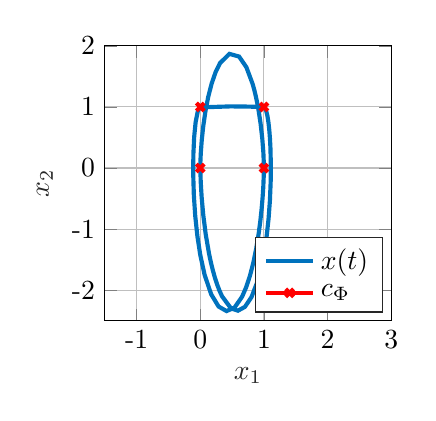
\begin{tikzpicture}

\begin{axis}[%
width=0.3\textwidth,
height=0.288\textwidth,
at={(0\textwidth,0\textwidth)},
scale only axis,
xmin=-1.5,
xmax=3,
xlabel style={font=\color{white!15!black}},
xlabel={$x_1$},
ymin=-2.5,
ymax=2,
ylabel style={font=\color{white!15!black}},
ylabel={$x_2$},
axis background/.style={fill=white},
xmajorgrids,
ymajorgrids,
legend style={at={(0.97,0.03)}, anchor=south east, legend cell align=left, align=left, draw=white!15!black},
xtick = {-1,0,...,3},xticklabels = {-1,0,...,3},ytick = {-2,-1,...,2.0},yticklabels = {-2,-1,...,2.0},
]
\addplot [color=mycolor1, line width=1.5pt]
  table[row sep=crcr]{%
-0.000536425622089443	-0.000253256143618596\\
0.000899826969557704	0.0780383035315735\\
0.00766750924998272	0.236863922047581\\
0.022865446171167	0.451703213214758\\
0.0466579403642906	0.683526854114203\\
0.0804723317443843	0.925557311349406\\
0.124395484386719	1.16208726143944\\
0.177902170942478	1.37965546100326\\
0.239951977195114	1.5670479269028\\
0.309081706105434	1.71529795468893\\
0.457110023240538	1.86832796722448\\
0.609644285740563	1.82404687696471\\
0.723808234554897	1.65075081733866\\
0.823210287031334	1.37409873463526\\
0.84919413181181	1.27533855128882\\
0.873188678436836	1.17111790369368\\
0.89510036476698	1.06262819903255\\
0.914854259919667	0.951172546773411\\
0.947731671984708	0.725086907193213\\
0.974746714506234	0.474544563051345\\
0.991126200123112	0.254288689824383\\
0.99991093595615	0.0393364101024569\\
1.00042347648345	0.00075249224958629\\
0.999444766611457	-0.0687934217650881\\
0.989863078018027	-0.313026700854836\\
0.979295922639339	-0.48052881975321\\
0.963968553380584	-0.667630010433671\\
0.943454706926384	-0.867027618348673\\
0.91751640926082	-1.07197639865858\\
0.879342799398558	-1.31567416867867\\
0.833524310319618	-1.54898601556016\\
0.780519454683227	-1.76346366072422\\
0.721048167635381	-1.95181406639466\\
0.656048988257108	-2.10790319375105\\
0.537484078992466	-2.28507993484256\\
0.412580530170511	-2.34085321199188\\
0.288060971976679	-2.26727851192337\\
0.170890029526908	-2.06579490312837\\
0.0677262459604298	-1.74698652996802\\
-0.000745981950729391	-1.41955947443041\\
-0.0457329973859744	-1.11281991145938\\
-0.0794131630903876	-0.783014496610158\\
-0.101173817291087	-0.441637785425257\\
-0.110831704243839	-0.10186685378701\\
-0.108700276049115	0.221403912437075\\
-0.0956529749904171	0.511550814830034\\
-0.0731837338934547	0.75023323115664\\
-0.0365432791820228	0.941478856604521\\
-0.00344686213827972	0.993227076992201\\
0.0415783855035543	0.993734249362652\\
0.470867843548952	1.00850927801934\\
0.6724486528192	1.00681506069602\\
0.999879665769405	0.999307186657998\\
1.00715928348142	0.995960594118129\\
1.01078340037518	0.992469907761963\\
1.03379684976849	0.94382536788466\\
1.05510655376311	0.852122197406093\\
1.07024407227643	0.752304561936894\\
1.0833127016857	0.632246246508452\\
1.09395251830735	0.495067555005041\\
1.10186695156037	0.343720116593714\\
1.10841885336523	0.0672414227321134\\
1.10595280835437	-0.228862020626158\\
1.09399407911028	-0.533181541239567\\
1.07243658451079	-0.835522386224152\\
1.04149170007436	-1.12687003285987\\
0.978872464632484	-1.52448333547969\\
0.898941230893278	-1.85809526434295\\
0.805149150349565	-2.11103494478474\\
0.701591234989397	-2.2718827321656\\
0.592763074135159	-2.33449483355815\\
0.483324723716747	-2.2980334385227\\
0.342240226664393	-2.09965027339199\\
0.302947068204721	-2.00997036916278\\
0.265486507678325	-1.90804728580842\\
0.230075367578805	-1.79505527682926\\
0.196917054281378	-1.6723124383553\\
0.166188173967997	-1.54128082006234\\
0.138032157899517	-1.40356731370554\\
0.085934181496814	-1.08803023350052\\
0.0471423354349039	-0.769824396204021\\
0.021282370317008	-0.472910994947978\\
0.00691430646607349	-0.224541342096751\\
0.000720723765911035	0.001612970134103\\
};
\addlegendentry{$x (t)$}

\addplot [color=red, line width=1.5pt, draw=none, mark=x, mark options={solid, red}]
  table[row sep=crcr]{%
0	0\\
1	0\\
0	1\\
1	1\\
};
\addlegendentry{$c_{\Phi}$}

\end{axis}
\end{tikzpicture}%
	\captionsetup{format=plain}
	\caption{Τροχιά $x(t)$ στο επίπεδο καταστάσεων $x_1 - x_2$ του Πειράματος \ref{subsec:rbf_siso}.}
	\label{fig:phase_plain}	
\end{wrapfigure}

\subsubsection{Αποτελέσματα}
Το σύστημα κλειστού βρόγχου που περιγράφεται στην προηγούμενη παράγραφο προσομοιώνεται για 300 περιόδους. Στο Σχήμα \ref{fig:siso_weights} παρουσιάζεται η χρονική εξέλιξη των βαρών $\hat{W}_{\varphi}(t)$ και $\hat{W}_{\gamma}(t)$ ενώ στο Σχήμα \ref{fig:phase_plain} απεικονίζεται η τροχιά $x(t)$ του συστήματος στο φασικό πορτραίτο $x_1$-$x_2$.

Όπως φαίνεται από το Σχήμα \ref{fig:siso_weights} τα βάρη των προσεγγίσεων συγκλίνουν στις τιμές των άγνωστων διανυσμάτων $W_\varphi^*$ και $W_\gamma^*$, συνεπώς το σχήμα αναγνώρισης πράγματι εκτιμά σωστά τις συναρτήσεις $\varphi(x)$ και $\gamma(x)$. Παρατηρούμε επίσης πως δεν έχουν όλα τα βάρη την ίδια ταχύτητα σύγκλισης, αφού τα βάρη $\hat{W}_{\gamma}(t)$ (δεξιά) συγκλίνουν πιο αργά από αυτά τα $\hat{W}_{\varphi}(t)$ (αριστερά).

}
%, συνεπώς απαιτείται έλεγχος κατά την λήψη της απόφασης του αν έχει 

Στο Σχήμα \ref{fig:phase_plain}, είναι φανερό ότι η τροχιά $x(t)$ διέρχεται από τα κέντρα $c_\Phi$ του διανύσματος οπισθοδρομητών $Z_\varphi(x)$, γεγονός που εξασφαλίζει την ικανοποίηση της Συνθήκης Επιμένουσας Διέγερσης. Παρομοίως, η ΣΕΔ επαληθεύεται και για το διάνυσμα οπισθοδρομητών $Z_\gamma(x)$ αφού τα κέντρα $c_\gamma$ αποτελούν την προβολή των κέντρων $c_\varphi$ στον $\mathbb{R}$.

Αξίζει να σημειωθεί πως σε αυτή την περίπτωση, καθώς η αρχιτεκτονική των δικτύων RBF που χρησιμοποιούνται στην αναγνώριση ταυτίζεται με τις μη γραμμικότητες του συστήματος, το αποτέλεσμα της προσέγγισης μπορεί να επεκταθεί σε ολόκληρο τον χώρο $\mathbb{R}^2$. Αν ωστόσο μελετούσαμε ένα πραγματικό σύστημα όπου οι μη γραμμικές του συναρτήσεις δεν δίνονται από αθροίσματα γκαουσιανών, τότε η προσέγγιση είναι τοπική και ισχύει μόνο σε μια γειτονιά των κέντρων των νευρωνικών δικτύων την οποία στην απόδειξη ορίζουμε ως $\Omega_x$. Παρόλα αυτά, όπως φαίνεται από το Σχήμα \ref{fig:phase_plain}, η περιοδική τροχιά $x(t)$ δεν βρίσκεται καθ' όλη την διάρκεια κοντά στα κέντρα του νευρωνικού δικτύου και κατά συνέπεια εντός αυτού του συμπαγούς συνόλου $\Omega_x$. Αυτός είναι και ο λόγος που στην απόδειξη του Κεφαλαίου \ref{chap:scheme_presentation}, διαχωρίζονται αυτά τα δυο σύνολα και μέσω υποθέσεων θεωρούμε πως ενώ οι προσεγγίσεις είναι τοπικές και ισχύουν μόνο για $x \in \Omega_x$, η τροχιά $x(t)$ είναι φραγμένη σε ένα συμπαγές σύνολο $\mathcal{X}$ το οποίο είναι υπερσύνολο του $\Omega_x$.

\subsection{Συστήματα ΠΕΠΕ}
\label{subsec:rbf_mimo}
Επεκτείνοντας το παραπάνω αποτέλεσμα για συστήματα ΠΕΠΕ, θεωρούμε το μη γραμμικό σύστημα:
\begin{equation*}
\label{eq:third_order_plant}
\begin{split}
\dot{x}_1 &= x_{2}  \\
\dot{x}_2 &= f_1(x) + g_{11}(x)u_1(t) + g_{12}(x)u_2(t) \\
\dot{x}_3 &= f_2(x) + g_{21}(x)u_1(t) + g_{22}(x)u_2(t)
\end{split}
\end{equation*}
όπου $x = \bmqty{x_1 & x_2 & x_3}^T$ το διάνυσμα καταστάσεων και $f_i : \mathbb{R}^3 \rightarrow \mathbb{R}$ και $g_{ij}:\mathbb{R} \rightarrow \mathbb{R}$ μη ομαλές συναρτήσεις που ικανοποιούν τις υποθέσεις του Κεφαλαίου \ref{chap:scheme_presentation}.

Όμοια με πριν, αρχικά ορίζουμε τις συναρτήσεις
\begin{equation*}
\begin{matrix}
\Phi(x) =  \begin{bmatrix}
\varphi_1(x) \\
\varphi_2(x)
\end{bmatrix}
& \text{και} \qquad  & \Gamma(x) = \begin{bmatrix}
\gamma_{11}(x) & \gamma_{12}(x) \\
\gamma_{21}(x) & \gamma_{22}(x)
\end{bmatrix}
\end{matrix}
\end{equation*}
όπου κάθε μια αποτελείται από τα άθροισμα γκαουσιανών των εξισώσεων \eqref{eq:mimo_zphi_def} - \eqref{eq:mimo_zgamma_def}, και στην συνέχεια ορίζουμε τις συναρτήσεις $f(x)$ και $G(x)$ ως
\begin{equation*}
\begin{matrix}
f(x) = \Gamma^{-1}(x) \Phi(x) \qquad
& \text{και} \qquad  & G(x) = \Gamma^{-1}(x)
\end{matrix}
\end{equation*}
όπου $f(x)$ και $G(x)$ ο συμβολισμός συμπαγής μορφής που χρησιμοποιείται και στην εξίσωση~\eqref{eq:mimo_compact} του Κεφαλαίου \ref{chap:scheme_presentation}.

\begin{equation}
	\varphi_i(x) = \sum_{k = 1}^{3} w_{\phi_{ik}}^* z_{\phi_k} (x) = W_{\varphi_i}^{*T} Z_\varphi(x), \quad i = 1,2
	\label{eq:mimo_zphi_def}
\end{equation}
\begin{equation}
\gamma_{ij}(x) = \sum_{k = 1}^{3} w_{\gamma_{ijk}}^* z_{\gamma_k} (x) = W_{\gamma_{ij}}^{*T} Z_{\gamma}(x), \quad i,j = 1,2
\label{eq:mimo_zgamma_def}
\end{equation}
Τα διανύσματα $Z_\Phi(x)$ και $Z_\Gamma(x)$ αποτελούνται από γκαουσιανές συναρτήσεις με κέντρα τα σημεία:
\begin{equation*}
\begin{matrix}
c_1 = \begin{bmatrix}  0.5 \\ 0.8 \\  0.2 \end{bmatrix}^Τ & \: \text{,} &
c_2 = \begin{bmatrix}  0.3 \\ 0.1 \\  0.5 \end{bmatrix} & \: \text{και} &
c_3 = \begin{bmatrix} -0.2 \\ 0.4 \\ -0.2 \end{bmatrix} 
\end{matrix}
\end{equation*}
και διασπορές $\sigma = 0.3$. Όπως και πριν, καθώς το σύστημα είναι τύπου \textit{Euler Lagrange} οι συναρτήσεις $z_{\phi_k}(x)$ είναι συνάρτηση της ποσότητας $\norm{x - c_k}$, δηλαδή του πλήρους διανύσματος καταστάσεων ενώ αντίθετα οι συναρτήσεις $z_{\gamma_k}(x)$ είναι συνάρτηση του $\abs{x_1 - c_{kx}}$, δηλαδή μόνο του $x_1$. Τέλος, τα βάρη κάθε $W_{\varphi_i}^{*}$ και $W_{\gamma_{ij}}^{*}$ κάθε συνάρτησης δίνονται στον Πίνακα \ref{tab:mimo_wstar}.
\begin{table}
	\centering
	\begin{tabular}{  c || r | r | r }
		\hline\hline
		\text{Συνάρτηση} & $w_{c_1}$ & $w_{c_2}$ & $w_{c_3}$ \\
		\hline\hline
		$\varphi_1(x)$ & $1$ & $2$ & $3$  \\ \hline
		$\varphi_2(x)$ & $4$ & $5$ & $6$  \\ \hline
		$\gamma_{11}(x)$ & $3$ & $0$ & $5$ \\ \hline
		$\gamma_{12}(x)$ & $1$ & $2$ & $3$ \\ \hline
		$\gamma_{21}(x)$ & $-1$ & $-2$ & $-3$ \\ \hline
		$\gamma_{22}(x)$ & $6$ & $7$ & $8$ \\ \hline \hline
	\end{tabular}
	\caption{$W_{\varphi_i}^{*}$ και $W_{\gamma_{ij}}^{*}$ του Πειράματος \ref{subsec:rbf_mimo}.}
	\label{tab:mimo_wstar}
\end{table}

{
\begin{wraptable}[18]{r}{0.3\textwidth}
	\centering
	\captionsetup{format=plain}
	\caption{Παράμετροι σχήματος αναγνώρισης για το Πείραμα \ref{subsec:rbf_mimo}}
	\begin{tabular}{ l | r }
		\hline\hline
		\text{Parameter}  & Value  \\ \hline\hline
		$k$               & $30$   \\ \hline
		$\lambda$         & $1 $   \\ \hline
		$\beta_{\varphi}$ & $0.4$  \\ \hline
		$\beta_{\gamma}$  & $0.2$  \\ \hline
		$\rho_0      $    & $4$    \\ \hline
		$\rho_\infty $    & $0.02$ \\ \hline
		$l           $    & $2$    \\ \hline
		$\textit{ΔΤ} $    & $1$    \\ \hline \hline	
	\end{tabular}
	\label{tab:rbf_mimo_params}
\end{wraptable}
\subsubsection{Σχήμα Αναγνώρισης}
Για την αναγνώριση των άγνωστων συναρτήσεων, όπως και στο προηγούμενο πείραμα θα χρησιμοποιηθούν νευρωνικά δίκτυα RBF ίδιας δομής με αυτά των $Z_\Phi$ και $Z_\Gamma$. Έτσι λοιπόν, σχηματίζουμε τις προσεγγίσεις:
\begin{equation*}
\hat{\Phi}(x,t)  =  
%\begin{bmatrix}
%\hat{\varphi}_1(x) \\
%\hat{\varphi}_2(x)
%\end{bmatrix}
\begin{bmatrix}
\hat{w}_{\varphi_1}(t)^T Z_\Phi(x) \\
\hat{w}_{\varphi_2}(t)^T Z_\Phi(x)
\end{bmatrix}
\end{equation*}
και
\begin{equation*}
\begin{matrix}
\hat{\Gamma}(x,t) = \begin{bmatrix}
\hat{w}_{\gamma_{11}}(t)^T Z_\Gamma(x) 
& \hat{w}_{\gamma_{12}}(t)^T Z_\Gamma(x) \\
\hat{w}_{\gamma_{21}}(t)^T Z_\Gamma(x) 
& \hat{w}_{\gamma_{22}}(t)^T Z_\Gamma(x) \\
\end{bmatrix}
\end{matrix}
\end{equation*}
Αντίστοιχα με το Πείραμα $\ref{subsec:rbf_siso}$, σύγκλιση των βαρών $\hat{w}_{\varphi_i}(t)$ και $\hat{w}_{\gamma_{ij}}(t)$, $i,j = 1,2$ στις αντίστοιχες τιμές του Πίνακα \ref{tab:rbf_mimo_params} συνεπάγεται σε επιτυχή αναγνώριση των άγνωστων συναρτήσεων του συστήματος. Τέλος, οι παράμετροι του σχήματος αναγνώρισης απεικονίζονται στον Πίνακα \ref{tab:rbf_mimo_params}.

}

{
\begin{wrapfigure}{r}{0.4\textwidth}
	%\centering
	% This file was created by matlab2tikz.
%
\definecolor{mycolor1}{rgb}{0.00000,0.44700,0.74100}%
\definecolor{mycolor2}{rgb}{1.00000,0.00000,1.00000}%
\definecolor{mycolor3}{rgb}{0.49000,1.00000,0.63000}%
%
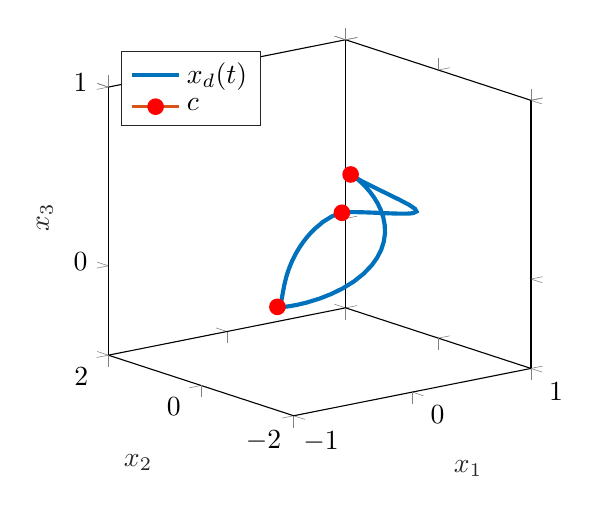
\begin{tikzpicture}

\begin{axis}[%
width=2.113in,
height=1.88in,
at={(0.589in,0.336in)},
scale only axis,
xmin=-1,
xmax=1,
tick align=outside,
xlabel style={font=\color{white!15!black}},
xlabel={$x_1$},
ymin=-2,
ymax=2,
ylabel style={font=\color{white!15!black}},
ylabel={$x_2$},
zmin=-0.5,
zmax=1,
zlabel style={font=\color{white!15!black}},
zlabel={$x_3$},
view={-38}{16},
axis background/.style={fill=white},
legend style={at={(0.03,0.97)}, anchor=north west, legend cell align=left, align=left, draw=white!15!black}
]
\addplot3 [color=mycolor1, line width=1.5pt]
 table[row sep=crcr] {%
-0.200974320547294	0.398240326057365	-0.200014956577444\\
-0.200974320547294	0.398240326057365	-0.200014956577444\\
-0.197891190130507	0.398662556556026	-0.199894761540088\\
-0.194801792113881	0.399556837930923	-0.199637509074269\\
-0.191702548615318	0.400915265833695	-0.199242362126494\\
-0.176601337303671	0.412699500748977	-0.195648085475245\\
-0.160906705630597	0.432682635678683	-0.1892278195571\\
-0.144358237077372	0.459286109429584	-0.180170665741969\\
-0.126739675957336	0.490884117676884	-0.168704973050285\\
-0.0937114026895122	0.552491923330419	-0.144153132188354\\
-0.0566572776979083	0.617655769538861	-0.114447058233437\\
-0.0155019645455458	0.680585955456736	-0.0808339654583171\\
0.00201308940901961	0.703925651748995	-0.0666229409699188\\
0.0200979005415358	0.725970588698077	-0.0520658296762162\\
0.0387170135855809	0.746528129143453	-0.0372396521044831\\
0.0578338531185452	0.765423151572908	-0.0222217778691167\\
0.0774063447925339	0.782513515330544	-0.00708982989826277\\
0.0886319831715183	0.79131438033762	0.00146793661360323\\
0.0999787102031805	0.799491625385024	0.0100233582369311\\
0.111437474240133	0.807033568290667	0.0185624905794462\\
0.122999194341946	0.813931085580778	0.02707139612148\\
0.13465467290953	0.820177976398265	0.0355361499533605\\
0.164699608646909	0.83314880512656	0.0568000397521517\\
0.195139883558379	0.841936958185377	0.0774569539647179\\
0.225826363708166	0.846705549282782	0.097276711650407\\
0.256617967258834	0.847750852387794	0.116029166405746\\
0.287386671634206	0.845499186113238	0.133484192646784\\
0.353954697423618	0.831984811938685	0.165953874806011\\
0.419203102964721	0.813442884472792	0.18875989400013\\
0.483130406013221	0.800633521819239	0.199511400943848\\
0.499996491599465	0.799860448786054	0.200037471156684\\
0.499996491599465	0.799860448786054	0.200037471156684\\
0.503887610290641	0.799008042688813	0.200073365636988\\
0.50777072634192	0.797193514896888	0.200150345036104\\
0.511641208693092	0.79442290542413	0.200268868587717\\
0.529859262024539	0.76982185995709	0.201360715537837\\
0.547282559130267	0.727032400459336	0.203337611651877\\
0.563532353951289	0.668401279229976	0.206169259087811\\
0.578267530778994	0.596466185266455	0.209814695875594\\
0.599221990604989	0.449408480769773	0.217805379863254\\
0.613914541311437	0.282037923567167	0.227819450137063\\
0.621702431976472	0.10503179608919	0.23962404169487\\
0.622807419498474	-0.0345821222033521	0.250003283878368\\
0.619583261582282	-0.170401584928941	0.261234098925449\\
0.612212208890114	-0.298953059602183	0.273206042856302\\
0.600969095929799	-0.417184841003779	0.285808511275454\\
0.586216355906217	-0.522488548179841	0.298930738811224\\
0.546049266115671	-0.691783399485713	0.327529764206098\\
0.497277115997444	-0.782535979421642	0.356903436948416\\
0.4452748233692	-0.790124895308415	0.386042210382328\\
0.395424417356792	-0.718517877620314	0.413936714777865\\
0.352543271830074	-0.580248258392495	0.439577413922316\\
0.320341551695358	-0.396428013009539	0.461954724403558\\
0.298673488522387	-0.161723405652703	0.482804489842069\\
0.293844363022617	-0.0073201228351173	0.493672411443225\\
0.296574258602398	0.0873920536445433	0.49936092982705\\
0.299222061140832	0.0998852532461457	0.50003510111031\\
0.299222061140832	0.0998852532461457	0.50003510111031\\
0.299393866185267	0.099777908975244	0.500024630260135\\
0.299565312282102	0.0995475969015495	0.500002070748539\\
0.299736187201349	0.0991930166814513	0.499967208833214\\
0.300656007999198	0.0952135916829193	0.499568986722109\\
0.301520685243967	0.0877691795372573	0.498810552449346\\
0.302299506957122	0.0770215635753541	0.497694151290167\\
0.302962051409463	0.0631682008253579	0.496225328912812\\
0.303694583658728	0.0361498890319874	0.493282523693491\\
0.303988812501078	0.00295526449975153	0.489542245936709\\
0.303757144708881	-0.0356721274880763	0.48503159096696\\
0.30292414812481	-0.0790224726616744	0.479777357290548\\
0.301425664278708	-0.12641959230636	0.47380595434198\\
0.295981412992011	-0.234637408234879	0.459276103011451\\
0.287103155074127	-0.35201736332168	0.442018173430834\\
0.274591835128835	-0.47358561142489	0.422265911549388\\
0.25839031883456	-0.594811518712421	0.400253598676377\\
0.238571125390103	-0.711619233804386	0.37621554716089\\
0.215323845276022	-0.820392967086564	0.350385799363365\\
0.184369413489948	-0.932621303908123	0.318404767639488\\
0.149787302599739	-1.02553828470373	0.284685262531027\\
0.112320819093465	-1.09578231832042	0.249595420477525\\
0.0728163133431375	-1.14082450090195	0.213503316997465\\
0.0321942873379919	-1.15896955294918	0.176776892560539\\
-0.00857952666939817	-1.14935574042719	0.139784009411843\\
-0.0578041024835539	-1.09919396267041	0.0941689623445227\\
-0.103948021351514	-1.0082761305377	0.049407451379967\\
-0.1453068594757	-0.880208173171665	0.00619778410420698\\
-0.180374211516195	-0.720606842607512	-0.0347615641793337\\
-0.207931320813986	-0.537066798986009	-0.0727720643011939\\
-0.229351068191364	-0.308260232708488	-0.112054174842132\\
-0.238191851493167	-0.118861558618627	-0.139864548758525\\
-0.239741198604411	0.0199242186023648	-0.158129793264245\\
-0.237079024741412	0.146578535125969	-0.173441146079101\\
-0.230692669263895	0.254705304125296	-0.185532709845526\\
-0.221272885544236	0.33739608693505	-0.194138409961781\\
-0.209738356397608	0.387196275918033	-0.198992235633557\\
-0.200974528429262	0.398239759539894	-0.2000149591164\\
};
 \addlegendentry{$x_d (t)$}

\addplot3 [color=mycolor2, line width=1.0pt, draw=none, mark size=2.5pt, mark=*, mark options={solid, fill=mycolor3, red}]
 table[row sep=crcr] {%
0.5	0.8	0.2\\
0.3	0.1	0.5\\
-0.2	0.4	-0.2\\
};
 \addlegendentry{$c$}

\end{axis}
\end{tikzpicture}%
	\captionsetup{format=plain}
	\caption{Τροχιά $x(t)$ και κέντρα RBF στο Πείραμα \ref{subsec:rbf_mimo}}
	\label{fig:phase_plain_mimo}	
\end{wrapfigure}
\subsubsection{Αποτελέσματα}
Το σύστημα προσομοιώθηκε για 2000 περιόδους, και στα Σχήματα \ref{fig:mimo_phi_weights}, \ref{fig:mimo_gamma1_weights} και \ref{fig:mimo_gamma2_weights} απεικονίζεται η εξέλιξη των βαρών κάθε RBF νευρωνικού δικτύου στον χρόνο. Συγκρίνοντας τις γραφικές αυτές με τον Πίνακα \ref{tab:mimo_wstar}, εύκολα επαληθεύεται πως τα βάρη συγκλίνουν στις σωστές τιμές. Τέλος, στο Σχήμα \ref{fig:phase_plain_mimo} φαίνεται η τρισδιάστατη τροχιά $x(t)$ στον $\mathbb{R}^3$ καθώς και τα κέντρα $c$. Από το σχήμα φαίνεται πως η τροχιά διέρχεται και από τα τρία κέντρα των οπισθοδρομητών και κατά συνέπεια ικανοποιεί την ΣΕΔ της Παραγράφου \ref{subsec:rbf_PE}.

}

\begin{figure}
	\begin{subfigure}{0.5\textwidth}
		% This file was created by matlab2tikz.
%
\definecolor{mycolor1}{rgb}{0.00000,0.44700,0.74100}%
\definecolor{mycolor2}{rgb}{0.85000,0.32500,0.09800}%
\definecolor{mycolor3}{rgb}{0.92900,0.69400,0.12500}%
%
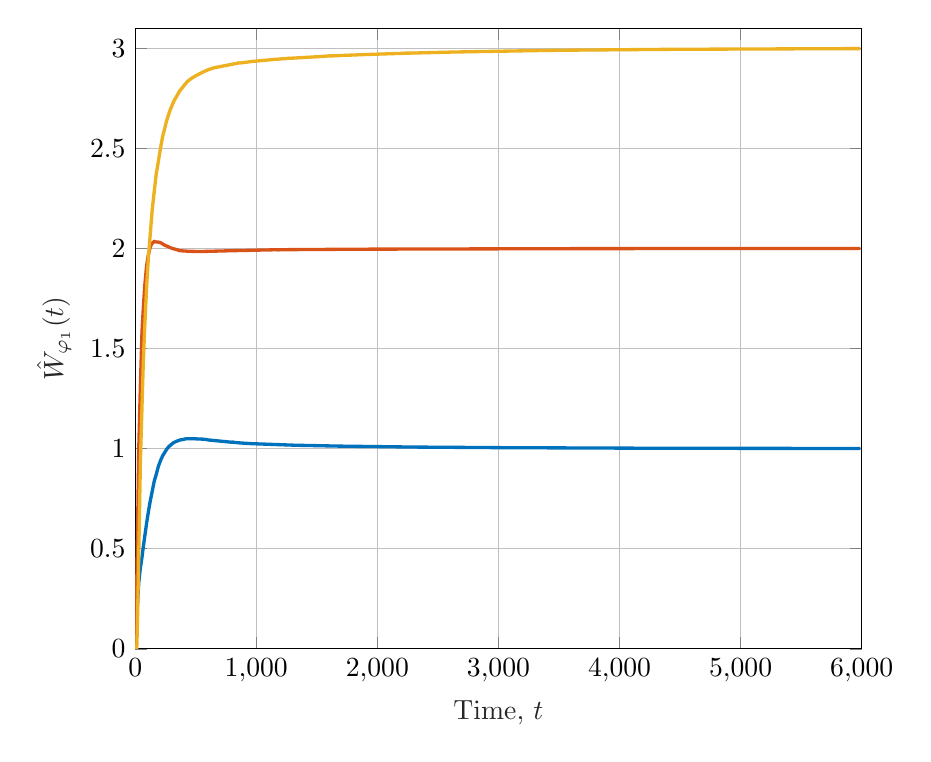
\begin{tikzpicture}

\begin{axis}[%
width=0.761\textwidth,
height=0.65\textwidth,
at={(0\textwidth,0\textwidth)},
scale only axis,
xmin=0,
xmax=6000,
xlabel style={font=\color{white!15!black}},
xlabel={Time, $t$},
ymin=0,
ymax=3.1,
ylabel style={font=\color{white!15!black}},
ylabel={$\hat{W}_{\varphi_1} (t)$},
axis background/.style={fill=white},
xmajorgrids,
ymajorgrids
]
\addplot [color=mycolor1, line width=1.2pt, forget plot]
  table[row sep=crcr]{%
0	0\\
8.82567774673498	0.11065720418992\\
19.0172805425273	0.221215639465299\\
29.8429018432244	0.331683833985153\\
43.2073612132581	0.40498131678396\\
56.5598050272929	0.457631533323365\\
67.4381941604706	0.510477209913006\\
94.2494444992581	0.626649760679356\\
109.745317186334	0.686819456021112\\
125.853275747037	0.742240644149206\\
142.009734557038	0.789999530547902\\
158.358176006041	0.839610697966236\\
174.711371588775	0.872236881542449\\
191.072830577384	0.910554330578634\\
209	0.939474785349375\\
226.168675099905	0.963378119886329\\
258.852456575039	0.995412681394555\\
274.37469863266	1.00817761184953\\
313.26064574162	1.02818733769709\\
338.638266648485	1.03607217593071\\
367.60143712086	1.04258054855291\\
424.644423402465	1.04947479508337\\
469.742592788507	1.04961164042288\\
573.920739656148	1.04684845539578\\
604.071614023123	1.04320818339966\\
793.009737402353	1.03209035033797\\
807.890949647943	1.0327082351705\\
822.594522065605	1.03078062430723\\
881.294893168033	1.02775027813186\\
968.739052843299	1.02455860934606\\
1297.79156238096	1.01744765536478\\
1326.38749168956	1.01687954589033\\
1683.36182621836	1.01251214212061\\
2302.12193825572	1.00777319546432\\
2331.02332908133	1.00764192174756\\
3029.13907617967	1.00476265140514\\
3083.94786295601	1.00460062227103\\
4195.32796351535	1.00210921387406\\
4341.00772231821	1.0018952671262\\
5750.05772439576	1.00077336212507\\
5989.14757750197	1.0006692664374\\
};
\addplot [color=mycolor2, line width=1.2pt, forget plot]
  table[row sep=crcr]{%
0	0\\
8.82567774673498	0.139886946558363\\
19.0172805425273	0.563465619089584\\
29.8429018432244	1.00353887942583\\
43.2073612132581	1.31810959061477\\
56.5598050272929	1.58618748695153\\
67.4381941604706	1.70419573945219\\
79.6566813477057	1.8176286377693\\
94.2494444992581	1.91213089224766\\
109.745317186334	1.97114249625429\\
125.853275747037	2.00924791124908\\
142.009734557038	2.02750370344529\\
158.358176006041	2.03481008954259\\
174.711371588775	2.03200712145826\\
191.072830577384	2.03155487112144\\
209	2.02902611148238\\
242.620196855619	2.0166078374059\\
302.51819529059	2.00080211491513\\
352.896711270768	1.99222609820299\\
367.60143712086	1.98877861878373\\
439.531122822289	1.98586969010375\\
529.414315658441	1.9844702574801\\
604.071614023123	1.98548844379729\\
793.009737402353	1.98856097674434\\
1154.44588994236	1.99326443039899\\
1183.966814416	1.99283296549311\\
1212.46277330087	1.99366758553333\\
1838.515459492	1.99617069398391\\
1880.96020294399	1.99627503731608\\
3648.01547412579	1.99892674599505\\
3817.15205514846	1.99907414836071\\
5296.16798022637	1.99967145106348\\
5895.13430030739	1.99974693686454\\
5989.14757750197	1.99974009220659\\
};
\addplot [color=mycolor3, line width=1.2pt, forget plot]
  table[row sep=crcr]{%
0	0\\
8.82567774673498	-0.0991360468251514\\
19.0172805425273	0.129687812833254\\
29.8429018432244	0.48006952436026\\
43.2073612132581	0.936641542793041\\
56.5598050272929	1.21320791457401\\
67.4381941604706	1.43443535415554\\
79.6566813477057	1.61577384876728\\
94.2494444992581	1.80487295415514\\
109.745317186334	1.95796300960592\\
125.853275747037	2.08046625882525\\
142.009734557038	2.20048265227706\\
158.358176006041	2.28993512028137\\
174.711371588775	2.37513422683878\\
191.072830577384	2.43236550029906\\
209	2.49970710434991\\
226.168675099905	2.55742327196367\\
242.620196855619	2.59609735081085\\
258.852456575039	2.63640752935589\\
289.014607951359	2.69222699483635\\
302.51819529059	2.71088774377222\\
313.26064574162	2.72698861822846\\
325.049033754998	2.74221420222148\\
338.638266648485	2.75517796125769\\
352.896711270768	2.77114302670361\\
367.60143712086	2.78623591994437\\
410.005138169928	2.81881611949575\\
424.644423402465	2.82911514099669\\
439.531122822289	2.83790432423029\\
469.742592788507	2.85142442855431\\
499.195713385834	2.86187374074962\\
529.414315658441	2.871698442058\\
558.981417999369	2.88071560430762\\
604.071614023123	2.89281028747882\\
651.525181688713	2.90250686518539\\
822.594522065605	2.92251751286949\\
837.463923677879	2.92373146119644\\
852.171747989612	2.92687791216304\\
866.889976855859	2.92627848605753\\
955.063897009115	2.93316493846032\\
1154.44588994236	2.94462974099042\\
1169.03326575125	2.94475778254309\\
1198.37007951098	2.94648951587169\\
1255.13578538528	2.94884171014201\\
1269.06017900686	2.95057701565293\\
1283.34361511721	2.94998325288543\\
1355.28745375198	2.95243919599852\\
1543.05942134483	2.95887590252732\\
1599.13444431504	2.96177185172564\\
1627.18460272661	2.9616585199683\\
1655.22948084283	2.96245199413079\\
1880.96020294399	2.96809914238202\\
2214.88592636115	2.97471829140704\\
2229.09762401548	2.97564549941126\\
2258.32535624231	2.97547171977658\\
2622.4647014881	2.9810042370973\\
3394.20480936636	2.98905509612996\\
3577.28511549234	2.99031771512182\\
4442.17558706036	2.99470928752362\\
5424.85918085976	2.99696159610448\\
5989.14757750197	2.99823515528442\\
};
\end{axis}
\end{tikzpicture}%
		%\caption{$\hat{W}_\varphi(t)$}
	\end{subfigure}
	\begin{subfigure}{0.5\textwidth}
		% This file was created by matlab2tikz.
%
\definecolor{mycolor1}{rgb}{0.00000,0.44700,0.74100}%
\definecolor{mycolor2}{rgb}{0.85000,0.32500,0.09800}%
\definecolor{mycolor3}{rgb}{0.92900,0.69400,0.12500}%
%
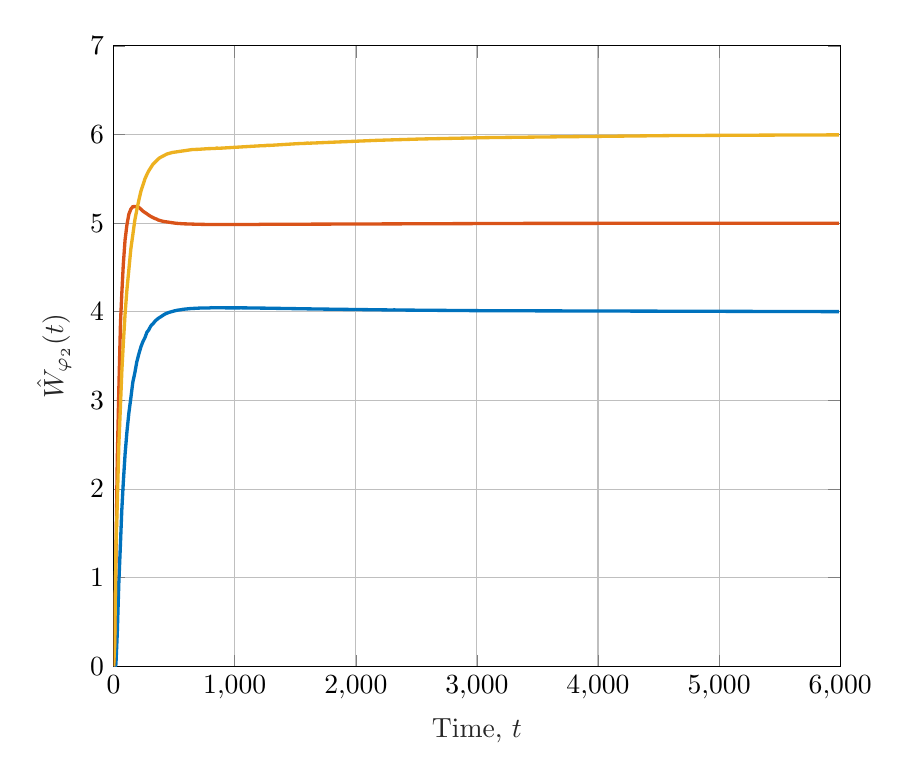
\begin{tikzpicture}

\begin{axis}[%
width=0.761\textwidth,
height=0.65\textwidth,
at={(0\textwidth,0\textwidth)},
scale only axis,
xmin=0,
xmax=6000,
xlabel style={font=\color{white!15!black}},
xlabel={Time, $t$},
ymin=0,
ymax=7,
ylabel style={font=\color{white!15!black}},
ylabel={$\hat{W}_{\varphi_2} (t)$},
axis background/.style={fill=white},
xmajorgrids,
ymajorgrids
]
\addplot [color=mycolor1, line width=1.2pt, forget plot]
  table[row sep=crcr]{%
0	0\\
8.82567774673498	-0.0405854968212225\\
19.0172805425273	0.0285558560899517\\
29.8429018432244	0.368890597575955\\
43.2073612132581	0.956146853729479\\
56.5598050272929	1.39421068382399\\
67.4381941604706	1.76471190365191\\
79.6566813477057	2.07425620773392\\
94.2494444992581	2.38926302300752\\
109.745317186334	2.64467837000666\\
125.853275747037	2.85929694271181\\
142.009734557038	3.02738750662138\\
158.358176006041	3.20552238321488\\
174.711371588775	3.30848695945224\\
191.072830577384	3.434182598181\\
209	3.52847688880502\\
226.168675099905	3.608263841189\\
242.620196855619	3.66562412937583\\
258.852456575039	3.70910820399604\\
274.37469863266	3.7682165326496\\
289.014607951359	3.79327410137284\\
302.51819529059	3.82892292578617\\
313.26064574162	3.85072515886714\\
325.049033754998	3.86493100422922\\
338.638266648485	3.8881434226987\\
352.896711270768	3.90759440602869\\
367.60143712086	3.924568765804\\
424.644423402465	3.97518723022495\\
454.191877487838	3.99152834865254\\
499.195713385834	4.00910876302623\\
529.414315658441	4.01797446890123\\
558.981417999369	4.02336437360009\\
573.920739656148	4.02804519118399\\
604.071614023123	4.0320324984541\\
635.086782732727	4.03611850775087\\
730.449154040343	4.04291939271388\\
793.009737402353	4.0432735888362\\
807.890949647943	4.04635066902392\\
852.171747989612	4.04514540955188\\
982.009737470965	4.04349681055555\\
1053.56405463394	4.04436498011819\\
1241.02402858683	4.04090724181242\\
1683.36182621836	4.03106113567537\\
2302.12193825572	4.02015773907988\\
2316.78392686985	4.02139123761208\\
2345.70735644431	4.01961293557815\\
3029.13907617967	4.01227268496223\\
3070.12489874842	4.01191299018774\\
5879.11625638215	4.00184708265533\\
5989.14757750197	4.00172351664605\\
};
\addplot [color=mycolor2, line width=1.2pt, forget plot]
  table[row sep=crcr]{%
0	0\\
8.82567774673498	0.286905749359903\\
19.0172805425273	1.25253145978058\\
29.8429018432244	2.32593379172431\\
43.2073612132581	3.14481112858721\\
56.5598050272929	3.87814547323615\\
67.4381941604706	4.20670323861486\\
79.6566813477057	4.53117845680663\\
94.2494444992581	4.80767147156621\\
109.745317186334	4.98207982948861\\
125.853275747037	5.10137842769473\\
142.009734557038	5.15743183195718\\
158.358176006041	5.18539113530187\\
174.711371588775	5.18676882200361\\
191.072830577384	5.18365653508226\\
209	5.17725919599343\\
242.620196855619	5.13454557245495\\
302.51819529059	5.07853554111807\\
325.049033754998	5.06278073102385\\
338.638266648485	5.05278250676747\\
352.896711270768	5.04677209643796\\
367.60143712086	5.03525128833462\\
410.005138169928	5.01917604811752\\
514.481507652563	4.99833007879897\\
573.920739656148	4.99222463460865\\
697.257892285397	4.98674253358604\\
793.009737402353	4.9842979783225\\
1183.966814416	4.98445689825712\\
1212.46277330087	4.98616205687813\\
3409.00973784076	4.99676659855413\\
5601.5162187656	4.99928679314689\\
5989.14757750197	4.99931379470308\\
};
\addplot [color=mycolor3, line width=1.2pt, forget plot]
  table[row sep=crcr]{%
0	0\\
8.82567774673498	0.241073098255583\\
19.0172805425273	1.33081114439574\\
29.8429018432244	1.82776824564371\\
43.2073612132581	2.5093438430722\\
56.5598050272929	2.94872905953798\\
67.4381941604706	3.3210257867886\\
79.6566813477057	3.63733009723092\\
94.2494444992581	3.97205885493986\\
109.745317186334	4.24992972671316\\
125.853275747037	4.47754738154526\\
142.009734557038	4.70902409982773\\
158.358176006041	4.86786788518566\\
174.711371588775	5.03158385639381\\
191.072830577384	5.14740490797249\\
209	5.26411233384079\\
226.168675099905	5.36485791794439\\
258.852456575039	5.50027844258511\\
274.37469863266	5.54781058221852\\
289.014607951359	5.58832000539223\\
325.049033754998	5.66459310083337\\
367.60143712086	5.72272945830173\\
381.438745694973	5.7374373950106\\
439.531122822289	5.77922093289453\\
485.003432151922	5.79687556982208\\
651.525181688713	5.8302483331654\\
697.257892285397	5.83222128295984\\
778.151535992266	5.83972337833984\\
837.463923677879	5.84203617756611\\
852.171747989612	5.84681416282456\\
866.889976855859	5.84380695262371\\
1183.966814416	5.86999259409731\\
1212.46277330087	5.87220802954926\\
1255.13578538528	5.87432319753225\\
1269.06017900686	5.87832826005251\\
1283.34361511721	5.87631803186923\\
1514.92850683944	5.89592202737094\\
1585.12356530643	5.89985646192963\\
1599.13444431504	5.90321995572867\\
1613.18400244325	5.90130476057948\\
2171.05696155931	5.93354577949412\\
2535	5.94869359845143\\
2608.01460651118	5.95092108778681\\
3083.94786295601	5.96441553083878\\
4600.00486914294	5.98746222686259\\
5568.41377043963	5.99359768912382\\
5989.14757750197	5.9953419122221\\
};
\end{axis}
\end{tikzpicture}%
		%\caption{$\hat{W}_\gamma(t)$)}
	\end{subfigure}
	\caption{ Χρονική εξέλιξη των βαρών $\hat{W}_{\varphi_1}(t)$ (αριστερά) και $\hat{W}_{\varphi_2}(t)$ (δεξιά) για το πείραμα \ref{subsec:rbf_mimo}}
	\label{fig:mimo_phi_weights}
\end{figure}

\begin{figure}
	\begin{subfigure}{0.5\textwidth}
		% This file was created by matlab2tikz.
%
\definecolor{mycolor1}{rgb}{0.00000,0.44700,0.74100}%
\definecolor{mycolor2}{rgb}{0.85000,0.32500,0.09800}%
\definecolor{mycolor3}{rgb}{0.92900,0.69400,0.12500}%
%
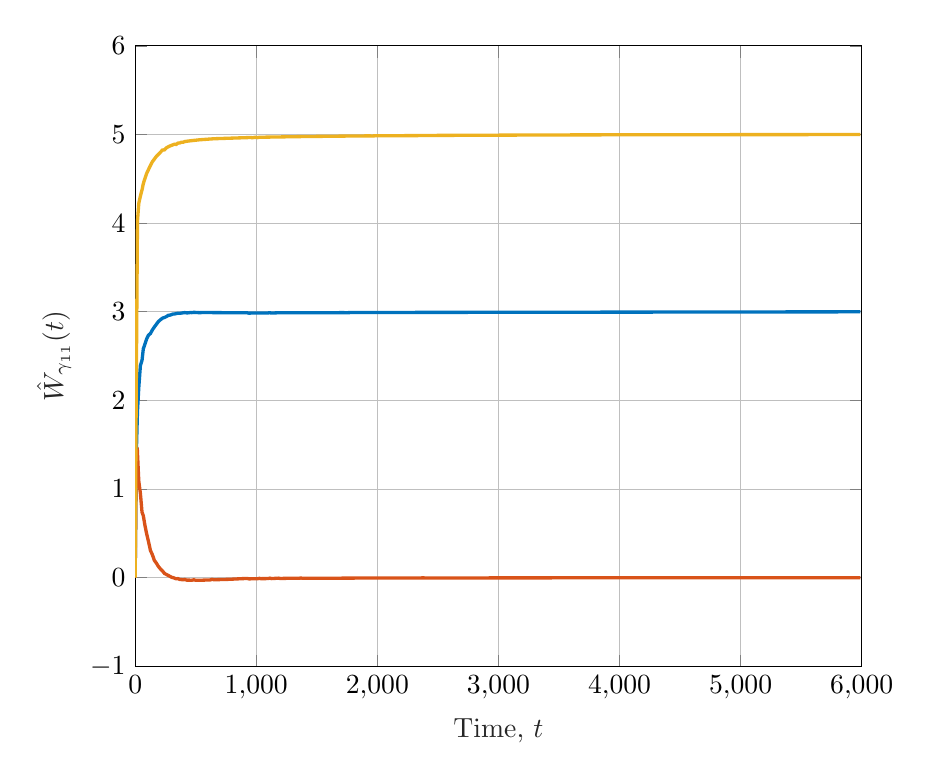
\begin{tikzpicture}

\begin{axis}[%
width=0.761\textwidth,
height=0.65\textwidth,
at={(0\textwidth,0\textwidth)},
scale only axis,
xmin=0,
xmax=6000,
xlabel style={font=\color{white!15!black}},
xlabel={Time, $t$},
ymin=-1,
ymax=6,
ylabel style={font=\color{white!15!black}},
ylabel={$\hat{W}_{\gamma_{11}} (t)$},
axis background/.style={fill=white},
xmajorgrids,
ymajorgrids
]
\addplot [color=mycolor1, line width=1.2pt, forget plot]
  table[row sep=crcr]{%
0	0\\
8.82567774673498	1.36696575731548\\
19.0172805425273	1.87813868334342\\
29.8429018432244	2.14529253992714\\
43.2073612132581	2.39382706516699\\
56.5598050272929	2.4516657959839\\
67.4381941604706	2.58285463841639\\
94.2494444992581	2.69189607284079\\
109.745317186334	2.73575063498993\\
125.853275747037	2.75404280497514\\
142.009734557038	2.7947599647141\\
158.358176006041	2.82818954325285\\
191.072830577384	2.88827621654764\\
209	2.91039122071834\\
226.168675099905	2.92795234092955\\
242.620196855619	2.93572880093598\\
258.852456575039	2.94659064160714\\
274.37469863266	2.96059547734876\\
289.014607951359	2.96246051278649\\
313.26064574162	2.97457091457181\\
325.049033754998	2.9750189424085\\
352.896711270768	2.98385007372872\\
367.60143712086	2.98269203704149\\
410.005138169928	2.99081243167802\\
424.644423402465	2.98765739606552\\
439.531122822289	2.98791555150819\\
454.191877487838	2.99093701655238\\
469.742592788507	2.99055700978715\\
485.003432151922	2.99373521150119\\
529.414315658441	2.98968794378834\\
558.981417999369	2.9914923344777\\
896.033408107633	2.98800685069\\
926.071906752755	2.98794234746219\\
940.652533654194	2.9841278235408\\
968.739052843299	2.98629463645011\\
1097.49475195213	2.98680899104784\\
1112.1414102175	2.98855931105481\\
1126.41322729571	2.98539149252883\\
1169.03326575125	2.98789092502375\\
1514.92850683944	2.98887454401574\\
1543.05942134483	2.98892810951384\\
1724.82559615905	2.99015064781452\\
1738.63604922471	2.98881465457634\\
1780.88227047121	2.99106586175822\\
1838.515459492	2.99090782178337\\
1895.27695719544	2.99193269285115\\
5989.14757750197	2.99948365197997\\
};
\addplot [color=mycolor2, line width=1.2pt, forget plot]
  table[row sep=crcr]{%
0	0\\
8.82567774673498	1.38505712321785\\
19.0172805425273	1.40996410740445\\
29.8429018432244	1.08990897350941\\
43.2073612132581	0.950838214100258\\
56.5598050272929	0.740126349733146\\
67.4381941604706	0.69802196668752\\
79.6566813477057	0.598971662050644\\
94.2494444992581	0.497902195182178\\
109.745317186334	0.410603832792731\\
125.853275747037	0.308466697398217\\
142.009734557038	0.260300321471732\\
158.358176006041	0.195555676979893\\
174.711371588775	0.16568759092479\\
191.072830577384	0.128476909790152\\
209	0.0985897362133983\\
226.168675099905	0.0753746268792383\\
242.620196855619	0.0478456438640933\\
302.51819529059	0.00432992017795186\\
313.26064574162	0.00113922618129436\\
338.638266648485	-0.0121220981973238\\
352.896711270768	-0.0102190751522357\\
367.60143712086	-0.0183935337126968\\
395.572165574109	-0.0233728698840423\\
410.005138169928	-0.0196164283352118\\
424.644423402465	-0.02684684317137\\
454.191877487838	-0.0275880539365971\\
469.742592788507	-0.0276188670932243\\
485.003432151922	-0.0234371611286406\\
499.195713385834	-0.0286580137099008\\
529.414315658441	-0.0289852724145021\\
589.009737285974	-0.0260293960582203\\
619.131785191333	-0.0249860080120925\\
635.086782732727	-0.018448724325026\\
651.525181688713	-0.0229648339391133\\
778.151535992266	-0.017922563416505\\
881.294893168033	-0.0106079808147115\\
926.071906752755	-0.00832024736700987\\
940.652533654194	-0.0131566339114215\\
996.463367962189	-0.0108401292245617\\
1010.7554882358	-0.011078536687819\\
1025.00342172574	-0.00695339671437978\\
1039	-0.0106812159165202\\
1097.49475195213	-0.00942232149009214\\
1112.1414102175	-0.00487084563428652\\
1126.41322729571	-0.00982707916864456\\
1183.966814416	-0.00495474064337031\\
1198.37007951098	-0.00839420006377622\\
1297.79156238096	-0.00546460782879876\\
1326.38749168956	-0.00661235603547539\\
1340.71556330274	-0.00694872330586804\\
1369.99410956871	-0.0036160503013889\\
1384.20268500634	-0.00646890522330068\\
1795.33103538518	-0.00451819026693556\\
1895.27695719544	-0.00219316039147088\\
2098.23740949429	-0.00352869867401751\\
2243.78407138241	-0.00327231828032382\\
2287.73425798115	-0.00282431095547508\\
2345.70735644431	-0.00305406349980331\\
2375.01445723503	-0.00146707017484005\\
2404.07302756365	-0.0029570644182968\\
3394.20480936636	-0.00136201413533854\\
3929.85609993254	-0.000934791383770062\\
3999.48876827697	-0.000857238632306689\\
5063.67139404937	-0.000420488549025322\\
5280.62920066875	-0.000352781270521518\\
5989.14757750197	-0.000225306519496371\\
};
\addplot [color=mycolor3, line width=1.2pt, forget plot]
  table[row sep=crcr]{%
0	0\\
8.82567774673498	2.09087142642511\\
19.0172805425273	4.02084879442737\\
29.8429018432244	4.22277026488518\\
43.2073612132581	4.3047860691604\\
56.5598050272929	4.37474506769831\\
67.4381941604706	4.44605725667861\\
79.6566813477057	4.49915628040344\\
94.2494444992581	4.55847286377048\\
125.853275747037	4.65022163982394\\
142.009734557038	4.69188741474591\\
174.711371588775	4.75186392776959\\
209	4.80011797866337\\
226.168675099905	4.82514232022731\\
242.620196855619	4.8264599545455\\
258.852456575039	4.85025130723261\\
289.014607951359	4.87119986609287\\
325.049033754998	4.89008880212441\\
338.638266648485	4.88756721555364\\
352.896711270768	4.90195743870026\\
367.60143712086	4.90383203753117\\
381.438745694973	4.91186932905293\\
395.572165574109	4.91213906403846\\
410.005138169928	4.92009536480055\\
454.191877487838	4.92834126694561\\
529.414315658441	4.93958303615545\\
651.525181688713	4.95179770292907\\
955.063897009115	4.96577233646531\\
968.739052843299	4.96256327239007\\
982.009737470965	4.96659336068024\\
996.463367962189	4.96722780944947\\
1010.7554882358	4.96438831682372\\
1025.00342172574	4.96836209822959\\
1384.20268500634	4.97628638791684\\
1711.33218555718	4.98128054903736\\
1738.63604922471	4.98163692216622\\
1938.36237587037	4.98419440961788\\
1952.70246020567	4.98259849648821\\
1981.94895954634	4.98475473419876\\
2447.64605787809	4.98800189553458\\
2491.56380624375	4.98926330743689\\
3450.87090311381	4.99451360489729\\
3506.35939208689	4.99460842937242\\
3759.23537996154	4.99546203623322\\
3845.48964906712	4.99568110975815\\
4311.94219224489	4.99697686982836\\
5989.14757750197	4.99904377203347\\
};
\end{axis}
\end{tikzpicture}%
		%\caption{$\hat{W}_\varphi(t)$}
	\end{subfigure}
	\begin{subfigure}{0.5\textwidth}
		% This file was created by matlab2tikz.
%
\definecolor{mycolor1}{rgb}{0.00000,0.44700,0.74100}%
\definecolor{mycolor2}{rgb}{0.85000,0.32500,0.09800}%
\definecolor{mycolor3}{rgb}{0.92900,0.69400,0.12500}%
%
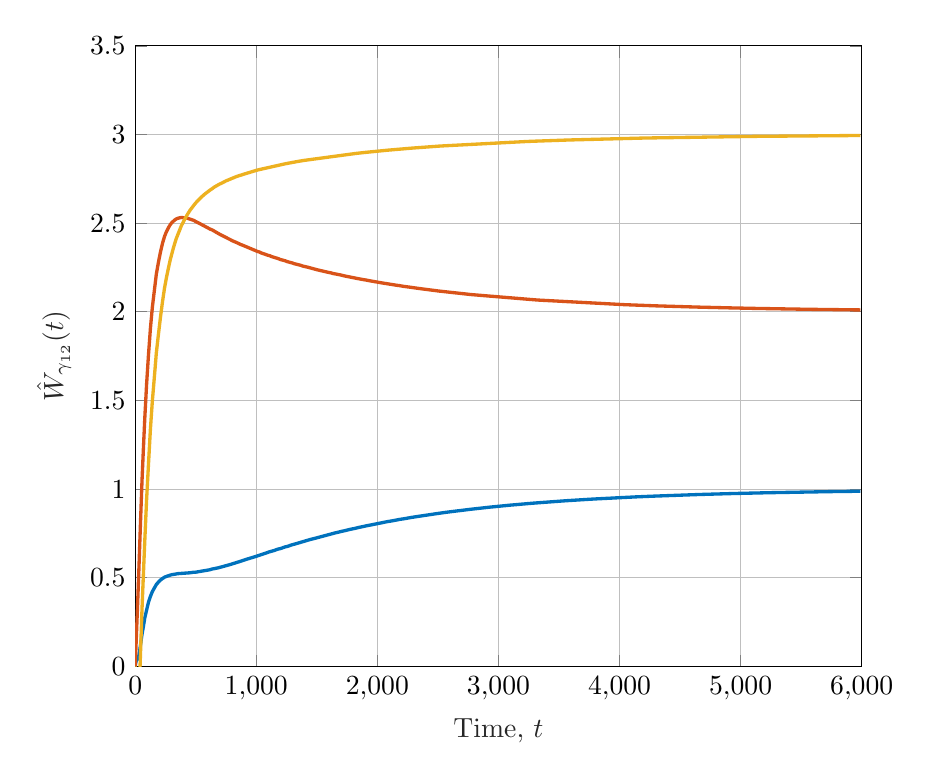
\begin{tikzpicture}

\begin{axis}[%
width=0.761\textwidth,
height=0.65\textwidth,
at={(0\textwidth,0\textwidth)},
scale only axis,
unbounded coords=jump,
xmin=0,
xmax=6000,
xlabel style={font=\color{white!15!black}},
xlabel={Time, $t$},
ymin=0,
ymax=3.5,
ylabel style={font=\color{white!15!black}},
ylabel={$\hat{W}_{\gamma_{12}} (t)$},
axis background/.style={fill=white},
xmajorgrids,
ymajorgrids
]
\addplot [color=mycolor1, line width=1.2pt, forget plot]
  table[row sep=crcr]{%
0	0\\
8.82567774673498	0.0327797907993954\\
19.0172805425273	0.0396295382797689\\
29.8429018432244	0.0576362147767213\\
43.2073612132581	0.115956620604265\\
56.5598050272929	0.180981340184189\\
67.4381941604706	0.222611983722345\\
79.6566813477057	0.274744618738623\\
109.745317186334	0.361560422586081\\
125.853275747037	0.394738289564884\\
142.009734557038	0.422032923954248\\
174.711371588775	0.461668045850274\\
191.072830577384	0.474721123932795\\
209	0.487277017105953\\
242.620196855619	0.503406366213312\\
274.37469863266	0.511475959939162\\
302.51819529059	0.517290631791184\\
325.049033754998	0.519644123705802\\
352.896711270768	0.523024422232993\\
454.191877487838	0.527984573722279\\
485.003432151922	0.531403457717715\\
499.195713385834	0.531293579749217\\
619.131785191333	0.545311499728996\\
635.086782732727	0.549082181039921\\
682.088946035951	0.555288439504693\\
730.449154040343	0.564202352969005\\
778.151535992266	0.573203367324822\\
866.889976855859	0.592059262138719\\
926.071906752755	0.605426199044814\\
996.463367962189	0.620112257261098\\
1112.1414102175	0.646760490270935\\
1140.56181414791	0.65216796153436\\
1183.966814416	0.662243643931106\\
1198.37007951098	0.664192478399855\\
1241.02402858683	0.674446237132543\\
1255.13578538528	0.676325928986444\\
1297.79156238096	0.686306858632634\\
1326.38749168956	0.691528561565974\\
1441.67294686879	0.714832209416272\\
1486.10068045336	0.722540525205659\\
1655.22948084283	0.753488573717732\\
1683.36182621836	0.757666953286389\\
1697.20603267102	0.760479977276191\\
1724.82559615905	0.764500337035315\\
1780.88227047121	0.773744266894937\\
1810.0097375071	0.777488591534166\\
1853	0.784720559619927\\
1880.96020294399	0.788433472139332\\
1909.94897891313	0.793034119856202\\
1938.36237587037	0.796629052718345\\
2083.89588192289	0.816583043297214\\
2112.98805135084	0.819652153774769\\
2185.81475078068	0.829131450573186\\
2214.88592636115	0.831984636274683\\
2287.73425798115	0.840805728970736\\
2331.02332908133	0.845286376011245\\
2491.56380624375	0.861712115197406\\
2564.18157882814	0.868789767884664\\
2759.63620938758	0.885228086293864\\
2853.55920616863	0.892401478378815\\
2924.258585045	0.897799702988777\\
3098	0.909462537053514\\
3153.38700486631	0.912694601596741\\
3265.94737611083	0.919451807820224\\
3336.13494846969	0.923139305540644\\
3563.11487992717	0.934528143468924\\
3648.01547412579	0.938164396932734\\
3788.05723148917	0.944011225964459\\
4139.0034108314	0.956159352928807\\
4297.25047441858	0.960575967687873\\
4658.39910775497	0.969434856648149\\
4945.9243204362	0.975039038197792\\
5235.36209578005	0.979572252343132\\
5750.05772439576	0.9857710317483\\
5989.14757750197	0.987850561551568\\
};
\addplot [color=mycolor2, line width=1.2pt, forget plot]
  table[row sep=crcr]{%
0	0\\
8.82567774673498	0.148583155225424\\
19.0172805425273	0.32894441582539\\
29.8429018432244	0.5295882320288\\
43.2073612132581	0.795576810154671\\
56.5598050272929	1.04865381251147\\
67.4381941604706	1.21970758066072\\
79.6566813477057	1.40191329072604\\
94.2494444992581	1.58952752986079\\
109.745317186334	1.75503817016943\\
125.853275747037	1.90538825521253\\
142.009734557038	2.02573761239364\\
174.711371588775	2.21195721790446\\
191.072830577384	2.27499504368916\\
209	2.33764213522318\\
226.168675099905	2.38714253278522\\
242.620196855619	2.42515887611717\\
258.852456575039	2.45265402919722\\
274.37469863266	2.47358917039946\\
289.014607951359	2.49067493622897\\
302.51819529059	2.50247656941974\\
325.049033754998	2.51668027876076\\
338.638266648485	2.5233391757838\\
352.896711270768	2.52738514010161\\
381.438745694973	2.53187320605866\\
424.644423402465	2.52864842133204\\
454.191877487838	2.52242052627753\\
485.003432151922	2.51509634469949\\
499.195713385834	2.50907771158018\\
529.414315658441	2.49886304925985\\
604.071614023123	2.47161821189547\\
619.131785191333	2.46608997845033\\
635.086782732727	2.46192605748729\\
697.257892285397	2.43747774580333\\
807.890949647943	2.3989171517851\\
837.463923677879	2.39045808900391\\
866.889976855859	2.38073740528216\\
896.033408107633	2.37296238168983\\
1010.7554882358	2.3400117594847\\
1025.00342172574	2.33737161774752\\
1039	2.33237514661869\\
1068	2.32569370614601\\
1097.49475195213	2.31821762379514\\
1112.1414102175	2.31611738398351\\
1126.41322729571	2.31139111558241\\
1183.966814416	2.29930332320146\\
1198.37007951098	2.29487069414608\\
1241.02402858683	2.28709044769039\\
1255.13578538528	2.28288049718594\\
1297.79156238096	2.27534314775676\\
1311.65627142704	2.27167728896075\\
1369.99410956871	2.26139550064636\\
1384.20268500634	2.2576335575086\\
1427.03325909142	2.25108402749447\\
1501.00486862834	2.23716104790128\\
1571.38614387203	2.22602772956634\\
1599.13444431504	2.22160303832607\\
1613.18400244325	2.2201856280999\\
1627.18460272661	2.21690596909684\\
1697.20603267102	2.20750636662706\\
1724.82559615905	2.20274050709213\\
1824.06048163814	2.18908255371571\\
1880.96020294399	2.18167438778528\\
1909.94897891313	2.17856739152467\\
1938.36237587037	2.17463016439524\\
2039.94274093853	2.16252353209074\\
2156.37531649316	2.14986580740151\\
2185.81475078068	2.14711822498157\\
2214.88592636115	2.14350861361345\\
2287.73425798115	2.13690118547402\\
2331.02332908133	2.13254295845218\\
2506.04379142415	2.11707492518235\\
2650.85118649742	2.10624521604132\\
2705.03331917403	2.10228541911238\\
2773.07210320797	2.09707392864311\\
3321.92259512344	2.06622642830916\\
4041.80421890589	2.04005762239467\\
4124.79688707602	2.03787915485645\\
4297.25047441858	2.03348028533583\\
4658.39910775497	2.02611603175774\\
4945.9243204362	2.02144956269149\\
5121.41188311348	2.01894118751534\\
5568.41377043963	2.01385454452338\\
5989.14757750197	2.01042702492941\\
};
\addplot [color=mycolor3, line width=1.2pt, forget plot]
  table[row sep=crcr]{%
0	0\\
8.82567774673498	-0.310541944251781\\
nan	nan\\
29.8429018432244	-0.207417653163247\\
43.2073612132581	0.0552568473794963\\
56.5598050272929	0.325547862324129\\
67.4381941604706	0.510157700436139\\
79.6566813477057	0.711691692325076\\
94.2494444992581	0.938282386996434\\
109.745317186334	1.13726113691064\\
125.853275747037	1.33748466054476\\
142.009734557038	1.49753261777823\\
158.358176006041	1.63009043048169\\
174.711371588775	1.76717453718993\\
191.072830577384	1.86636624256244\\
209	1.96960305017274\\
226.168675099905	2.05906578838767\\
242.620196855619	2.13450544914849\\
258.852456575039	2.19484349480172\\
274.37469863266	2.24543386553614\\
289.014607951359	2.29128028729338\\
313.26064574162	2.35395259028701\\
325.049033754998	2.38149819330374\\
338.638266648485	2.41144966986758\\
381.438745694973	2.48520080998424\\
410.005138169928	2.52233078544577\\
424.644423402465	2.54088619653339\\
439.531122822289	2.55806133058559\\
454.191877487838	2.57350221925844\\
485.003432151922	2.60104414159196\\
499.195713385834	2.61339502122155\\
544.014605953697	2.64506159085431\\
573.920739656148	2.66310233776767\\
619.131785191333	2.68678814308259\\
635.086782732727	2.69377847127907\\
651.525181688713	2.70243261105134\\
697.257892285397	2.72023710702706\\
713.50755487906	2.7249848496549\\
746.801469872386	2.73715928600086\\
837.463923677879	2.76291736496842\\
911.25703472074	2.77894224814372\\
1010.7554882358	2.79957137084057\\
1241.02402858683	2.83484553971448\\
1340.71556330274	2.84747520813835\\
1398.36264972659	2.85399017287727\\
1824.06048163814	2.8930689980034\\
1895.27695719544	2.89841822821654\\
2083.89588192289	2.91123321119812\\
2287.73425798115	2.92311826470359\\
2520.56685863806	2.93478687158131\\
3237.48815018133	2.96046577796915\\
3336.13494846969	2.96300449512819\\
3591.53959350492	2.96903759059114\\
4209.72169598024	2.9799436412959\\
5135.85561430633	2.98939889018129\\
5925.46286126612	2.99384888848454\\
5989.14757750197	2.99412049130115\\
};
\end{axis}
\end{tikzpicture}%
		%\caption{$\hat{W}_\gamma(t)$)}
	\end{subfigure}
	\caption{ Χρονική εξέλιξη των βαρών $\hat{W}_{\gamma_{11}}(t)$ (αριστερά) και $\hat{W}_{\gamma_{12}}(t)$ (δεξιά) για το πείραμα \ref{subsec:rbf_mimo}}
		\label{fig:mimo_gamma1_weights}
	\end{figure}

\begin{figure}
	\begin{subfigure}{0.5\textwidth}
		% This file was created by matlab2tikz.
%
\definecolor{mycolor1}{rgb}{0.00000,0.44700,0.74100}%
\definecolor{mycolor2}{rgb}{0.85000,0.32500,0.09800}%
\definecolor{mycolor3}{rgb}{0.92900,0.69400,0.12500}%
%
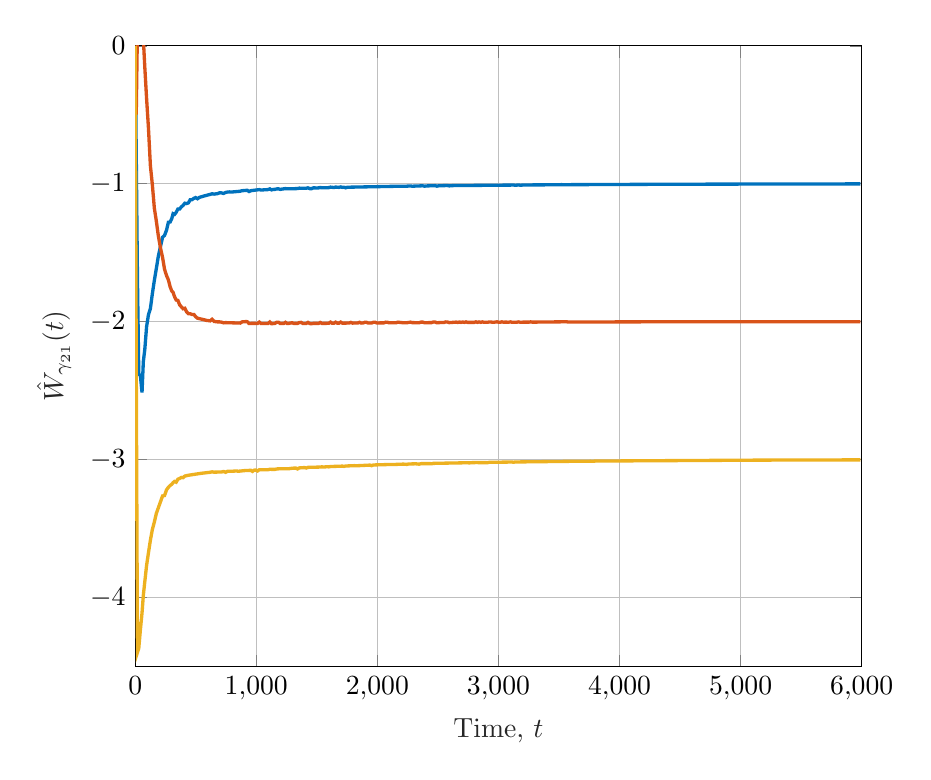
\begin{tikzpicture}

\begin{axis}[%
width=0.761\textwidth,
height=0.65\textwidth,
at={(0\textwidth,0\textwidth)},
scale only axis,
unbounded coords=jump,
xmin=0,
xmax=6000,
xlabel style={font=\color{white!15!black}},
xlabel={Time, $t$},
ymin=-4.5,
ymax=0,
ylabel style={font=\color{white!15!black}},
ylabel={$\hat{W}_{\gamma_{21}} (t)$},
axis background/.style={fill=white},
xmajorgrids,
ymajorgrids
]
\addplot [color=mycolor1, line width=1.2pt, forget plot]
  table[row sep=crcr]{%
0	0\\
8.82567774673498	-0.783373807902535\\
19.0172805425273	-1.69680330831761\\
29.8429018432244	-2.38007723803912\\
43.2073612132581	-2.39177205711258\\
56.5598050272929	-2.51407776008455\\
67.4381941604706	-2.29018254534276\\
79.6566813477057	-2.20073359042453\\
94.2494444992581	-2.03749968469765\\
109.745317186334	-1.94983608221264\\
125.853275747037	-1.90489587998218\\
142.009734557038	-1.79722915222283\\
158.358176006041	-1.70119673671525\\
174.711371588775	-1.61552762108022\\
191.072830577384	-1.5269536684882\\
226.168675099905	-1.38847750852528\\
242.620196855619	-1.37464103536786\\
258.852456575039	-1.33731382246879\\
274.37469863266	-1.27958017735455\\
289.014607951359	-1.27746910280439\\
302.51819529059	-1.2521743094112\\
313.26064574162	-1.21735209832423\\
325.049033754998	-1.2223061753848\\
338.638266648485	-1.2075425833018\\
352.896711270768	-1.18329322450245\\
367.60143712086	-1.1831143636964\\
381.438745694973	-1.16797477243654\\
395.572165574109	-1.15745471656101\\
410.005138169928	-1.14161434628477\\
424.644423402465	-1.14393717007533\\
439.531122822289	-1.13903250098974\\
454.191877487838	-1.11661583063687\\
469.742592788507	-1.11577336530172\\
485.003432151922	-1.105830986211\\
499.195713385834	-1.10060536557467\\
514.481507652563	-1.10879115675198\\
529.414315658441	-1.0997402630137\\
558.981417999369	-1.09138365381114\\
619.131785191333	-1.07748179042301\\
635.086782732727	-1.07265661879137\\
651.525181688713	-1.07542875619765\\
682.088946035951	-1.07159980345386\\
697.257892285397	-1.06560144579362\\
713.50755487906	-1.06673032532399\\
730.449154040343	-1.07066298349309\\
746.801469872386	-1.06349198042335\\
763.157774875984	-1.06023566421754\\
778.151535992266	-1.0592619499439\\
793.009737402353	-1.06052237397489\\
866.889976855859	-1.05466992340916\\
881.294893168033	-1.05080114974771\\
926.071906752755	-1.0476513409194\\
940.652533654194	-1.05639057600092\\
955.063897009115	-1.05068516156371\\
1025.00342172574	-1.04277405629728\\
1039	-1.04580518407147\\
1097.49475195213	-1.04248059119072\\
1112.1414102175	-1.03745807860923\\
1126.41322729571	-1.04472152737253\\
1140.56181414791	-1.04139491544083\\
1154.44588994236	-1.0410130952705\\
1169.03326575125	-1.03765914381438\\
1183.966814416	-1.03742805987076\\
1198.37007951098	-1.0409704490985\\
1241.02402858683	-1.03515304550911\\
1255.13578538528	-1.03713286430047\\
1311.65627142704	-1.03618961218217\\
1340.71556330274	-1.03510038478271\\
1355.28745375198	-1.03222021950478\\
1384.20268500634	-1.03239843013944\\
1412.61879387638	-1.03280219986209\\
1427.03325909142	-1.02996957013784\\
1441.67294686879	-1.03546359151005\\
1456.46666712834	-1.03575717674994\\
1471.24306922146	-1.02991997353638\\
1501.00486862834	-1.03087875881192\\
1514.92850683944	-1.03020550173824\\
1529.03321780063	-1.02754586725678\\
1543.05942134483	-1.02987671707706\\
1599.13444431504	-1.02845854778661\\
1613.18400244325	-1.02469321009085\\
1641.23495399155	-1.02750477701284\\
1655.22948084283	-1.0242683691049\\
1683.36182621836	-1.02666949632385\\
1697.20603267102	-1.02333568042013\\
1711.33218555718	-1.02627542230948\\
1724.82559615905	-1.02603370071301\\
1738.63604922471	-1.02943935981693\\
1752.41279945791	-1.02547886731645\\
2200.17097302751	-1.01787919720209\\
2243.78407138241	-1.01780871146548\\
2273.03315785021	-1.01611167755073\\
2287.73425798115	-1.01815115044428\\
2316.78392686985	-1.01701952690382\\
2375.01445723503	-1.01504194395056\\
2389.65384328071	-1.01819361044727\\
2404.07302756365	-1.0161361548553\\
2477.00340495577	-1.01401847017587\\
2491.56380624375	-1.01768111636375\\
2506.04379142415	-1.01506785710808\\
2579	-1.01305043477259\\
2593.45728838536	-1.01574735048689\\
2622.4647014881	-1.01364449769517\\
3125.75034119448	-1.00980083262584\\
3139.53190930965	-1.01135105694175\\
3167.29172021694	-1.00889391229248\\
3181.59255001596	-1.01099622478705\\
3209.37626480271	-1.00907764492331\\
3350.76962822865	-1.00831273682616\\
3379.76860309035	-1.00824195316818\\
3437.02385377629	-1.00722493076046\\
3464.77122280644	-1.0077179389682\\
3521.08602540496	-1.00679219981248\\
3549	-1.00729050875543\\
3577.28511549234	-1.00693254714406\\
3689.9495564209	-1.00661240621048\\
3731.66793226712	-1.00642246538155\\
3773.6904080767	-1.00621680136919\\
3817.15205514846	-1.00588290240103\\
4013.97741117061	-1.00526579415964\\
4069	-1.00511069424556\\
4399.18760949767	-1.00395694318195\\
4570.66404188551	-1.00399822166946\\
4614.4130757496	-1.00342344126329\\
5193	-1.00232534650331\\
5312.01463252907	-1.00197582719284\\
5488.514221561	-1.00219280749661\\
5552.14648774913	-1.00159974829148\\
5701.57544467955	-1.00188099879688\\
5814.38701260355	-1.00146825784304\\
5989.14757750197	-1.00132896592004\\
};
\addplot [color=mycolor2, line width=1.2pt, forget plot]
  table[row sep=crcr]{%
0	0\\
8.82567774673498	-0.498677764301647\\
19.0172805425273	0.141112004807837\\
nan	nan\\
67.4381941604706	0.0510643381476257\\
79.6566813477057	-0.156425240919816\\
94.2494444992581	-0.380846870568348\\
109.745317186334	-0.596388292264237\\
125.853275747037	-0.870607387854761\\
142.009734557038	-1.00759350287262\\
158.358176006041	-1.17748197087803\\
174.711371588775	-1.27036628517908\\
191.072830577384	-1.3759743438668\\
209	-1.46614026695988\\
226.168675099905	-1.53435487930255\\
242.620196855619	-1.62059749649234\\
258.852456575039	-1.66560392894098\\
274.37469863266	-1.6977727518688\\
289.014607951359	-1.74764608407349\\
302.51819529059	-1.77862274279414\\
313.26064574162	-1.78763556071408\\
325.049033754998	-1.81842810707803\\
338.638266648485	-1.84337241270441\\
352.896711270768	-1.84603700046864\\
367.60143712086	-1.87887876653986\\
395.572165574109	-1.90654019878639\\
410.005138169928	-1.90341392500159\\
424.644423402465	-1.92897538459329\\
439.531122822289	-1.94234830775167\\
454.191877487838	-1.94280676238304\\
469.742592788507	-1.94817556795988\\
485.003432151922	-1.9479112891986\\
499.195713385834	-1.96437259134564\\
514.481507652563	-1.97498707957766\\
544.014605953697	-1.98129805129338\\
589.009737285974	-1.99089095408453\\
619.131785191333	-1.99455673988086\\
635.086782732727	-1.98320002721994\\
651.525181688713	-1.99860017805622\\
682.088946035951	-2.00196643888285\\
697.257892285397	-2.00183997792101\\
713.50755487906	-2.00395907228813\\
730.449154040343	-2.00884157425571\\
746.801469872386	-2.0072879613117\\
866.889976855859	-2.01062966651352\\
881.294893168033	-2.00209822733632\\
911.25703472074	-1.99992660344469\\
926.071906752755	-2.00035804020808\\
940.652533654194	-2.01364140687838\\
968.739052843299	-2.01248714656049\\
1010.7554882358	-2.01327384743217\\
1025.00342172574	-2.00353431548047\\
1039	-2.01398752665864\\
1097.49475195213	-2.01338472976204\\
1112.1414102175	-2.00251426876457\\
1126.41322729571	-2.01545517986051\\
1154.44588994236	-2.01278829668536\\
1169.03326575125	-2.00434273023257\\
1183.966814416	-2.00471291744907\\
1198.37007951098	-2.0138970811231\\
1212.46277330087	-2.01276796026468\\
1226.86070587678	-2.01333478019387\\
1241.02402858683	-2.00489715644289\\
1255.13578538528	-2.01338153256529\\
1269.06017900686	-2.01325941470623\\
1283.34361511721	-2.00955618294302\\
1297.79156238096	-2.00891545907143\\
1311.65627142704	-2.01337948868968\\
1326.38749168956	-2.01248418411251\\
1340.71556330274	-2.01356234955711\\
1355.28745375198	-2.00651769902834\\
1369.99410956871	-2.005560464675\\
1384.20268500634	-2.01301772298848\\
1412.61879387638	-2.01335209722492\\
1427.03325909142	-2.00592629575112\\
1441.67294686879	-2.01415341449592\\
1456.46666712834	-2.01533091661531\\
1471.24306922146	-2.01287639919974\\
1514.92850683944	-2.01300246835854\\
1529.03321780063	-2.0059413684894\\
1543.05942134483	-2.01312897704065\\
1599.13444431504	-2.0121586269488\\
1613.18400244325	-2.00348699940059\\
1627.18460272661	-2.0116485185581\\
1641.23495399155	-2.0116900022249\\
1655.22948084283	-2.00399623578505\\
1669.25203725491	-2.0112559697709\\
1683.36182621836	-2.01103430329476\\
1697.20603267102	-2.00350389566938\\
1711.33218555718	-2.01133596267391\\
1766.43174815952	-2.01021203889013\\
1780.88227047121	-2.00555764048113\\
1795.33103538518	-2.0107073328536\\
1838.515459492	-2.01010151763148\\
1853	-2.0049602559393\\
1867.01460627968	-2.01060199719632\\
1880.96020294399	-2.01023956208519\\
1895.27695719544	-2.00509480021901\\
1909.94897891313	-2.00489349176223\\
1924.09772404188	-2.01020203886219\\
1952.70246020567	-2.00999454229168\\
1967.2770097797	-2.00495442112788\\
1981.94895954634	-2.00475044381255\\
1996.32104254865	-2.00967563193535\\
2054.43185498232	-2.00885098772596\\
2069.08586904938	-2.00397146925752\\
2083.89588192289	-2.0048531509201\\
2098.23740949429	-2.00881770403612\\
2141.8638402422	-2.00876436967246\\
2156.37531649316	-2.00751821813901\\
2171.05696155931	-2.00402424606546\\
2214.88592636115	-2.0084648186903\\
2243.78407138241	-2.00824274939077\\
2273.03315785021	-2.00387521570246\\
2287.73425798115	-2.00709608640136\\
2316.78392686985	-2.00783202143066\\
2345.70735644431	-2.00769465363646\\
2360.27568408568	-2.00379894854905\\
2375.01445723503	-2.00363110077706\\
2389.65384328071	-2.00809812809348\\
2447.64605787809	-2.00708862755982\\
2462.22623589561	-2.00256100301976\\
2477.00340495577	-2.00337553084228\\
2491.56380624375	-2.00821880084368\\
2520.56685863806	-2.00660342726314\\
2549.58426199838	-2.00643649574613\\
2564.18157882814	-2.00211673058766\\
2579	-2.00315077539199\\
2593.45728838536	-2.00725319061712\\
2650.85118649742	-2.00355873928311\\
2664.13453607567	-2.00594179618747\\
2678.00170908717	-2.00277016091604\\
2691.48901032321	-2.00552674972823\\
2705.03331917403	-2.00263037385957\\
2718.52118692228	-2.00542069040148\\
2732.20544345641	-2.00171166372547\\
2746.01460681554	-2.00560899560605\\
2800	-2.00537337903916\\
2813.20667841498	-2.00159680149682\\
2826.64982462691	-2.00519286875533\\
2840.05706883467	-2.00221681881158\\
2853.55920616863	-2.00495514859995\\
2867.07155187111	-2.002091654992\\
2881.00486886656	-2.0051088986811\\
2909.68374238925	-2.00502952217448\\
2924.258585045	-2.00214218732253\\
2938.90376583193	-2.00249397274547\\
2951.83771723017	-2.00482824797928\\
2965.05744143857	-2.00481720285097\\
2978.03322709389	-2.00215247880897\\
2990.26023556482	-2.00200850650799\\
3002.67746572809	-2.00464255180032\\
3015.46330865408	-2.0043860764099\\
3029.13907617967	-2.00151224851197\\
3042.73089441818	-2.0045311559561\\
3056.34319374593	-2.00338136536448\\
3083.94786295601	-2.00432937590358\\
3098	-2.00200139374465\\
3112	-2.0043210741178\\
3153.38700486631	-2.00394811000024\\
3167.29172021694	-2.0022326383114\\
3181.59255001596	-2.00481196101373\\
3209.37626480271	-2.00344392715397\\
3251.53622814238	-2.00367496390572\\
3265.94737611083	-2.00177516780423\\
3279.72981127921	-2.00378591442404\\
3563.11487992717	-2.00112959709804\\
3577.28511549234	-2.00302063982963\\
4556.00171191214	-2.00067763985044\\
4585.1967592351	-2.00147205472513\\
4760.76994238981	-2.00138668472846\\
4789.01460755076	-2.00137210553476\\
5393.10155883834	-2.00033493296633\\
5456.41598972765	-2.00078848954035\\
5989.14757750197	-2.0005763142517\\
};
\addplot [color=mycolor3, line width=1.2pt, forget plot]
  table[row sep=crcr]{%
0	0\\
8.82567774673498	-2.29317513938986\\
19.0172805425273	-4.39780564290595\\
29.8429018432244	-4.36800166246394\\
43.2073612132581	-4.23414801003582\\
56.5598050272929	-4.11330103526871\\
67.4381941604706	-3.98459977353377\\
79.6566813477057	-3.8849431059225\\
94.2494444992581	-3.76818373183414\\
109.745317186334	-3.67613613325102\\
125.853275747037	-3.58436358580275\\
142.009734557038	-3.50730228849625\\
158.358176006041	-3.45346321773195\\
174.711371588775	-3.391113896143\\
226.168675099905	-3.2642205438151\\
242.620196855619	-3.26105048567479\\
258.852456575039	-3.22025364439105\\
274.37469863266	-3.20120949679404\\
289.014607951359	-3.1879405412983\\
302.51819529059	-3.17917993147694\\
313.26064574162	-3.16746972488363\\
325.049033754998	-3.15896619242449\\
338.638266648485	-3.16417609604832\\
352.896711270768	-3.14272923728458\\
367.60143712086	-3.13714545687435\\
381.438745694973	-3.1297822832239\\
395.572165574109	-3.13153281476116\\
410.005138169928	-3.11992819530315\\
439.531122822289	-3.11408221800502\\
544.014605953697	-3.10006827374491\\
619.131785191333	-3.092326737652\\
635.086782732727	-3.08917516415931\\
651.525181688713	-3.0916970516364\\
713.50755487906	-3.09020905417674\\
730.449154040343	-3.08674611489732\\
746.801469872386	-3.0923113472445\\
763.157774875984	-3.08522978380097\\
807.890949647943	-3.08458593883188\\
837.463923677879	-3.08297989510902\\
852.171747989612	-3.08509659807532\\
911.25703472074	-3.07957650320986\\
955.063897009115	-3.07852982083205\\
968.739052843299	-3.08605796984375\\
982.009737470965	-3.07733208519494\\
996.463367962189	-3.07619136887661\\
1010.7554882358	-3.08298591218499\\
1025.00342172574	-3.07421987698126\\
1097.49475195213	-3.07348591125356\\
1112.1414102175	-3.07096964549874\\
1154.44588994236	-3.07161091489797\\
1169.03326575125	-3.06827064620302\\
1198.37007951098	-3.06673663239872\\
1269.06017900686	-3.0667982040859\\
1297.79156238096	-3.06289400600235\\
1326.38749168956	-3.06186495253678\\
1340.71556330274	-3.06832384888548\\
1355.28745375198	-3.06082551079544\\
1398.36264972659	-3.05827887261512\\
1412.61879387638	-3.06177493516043\\
1427.03325909142	-3.05684261851638\\
1514.92850683944	-3.05497293576627\\
1543.05942134483	-3.05309014705927\\
1557	-3.05447735820599\\
1585.12356530643	-3.05201045253398\\
1599.13444431504	-3.05321097664728\\
1613.18400244325	-3.05057357473197\\
1669.25203725491	-3.04922849311424\\
1711.33218555718	-3.04774335510956\\
1724.82559615905	-3.04963513812436\\
1738.63604922471	-3.04691906258449\\
1810.0097375071	-3.04434701222181\\
1824.06048163814	-3.04536480554543\\
1938.36237587037	-3.04038168316492\\
1952.70246020567	-3.04442961489349\\
1967.2770097797	-3.03944872541797\\
2112.98805135084	-3.03570121911525\\
2141.8638402422	-3.03579246431127\\
2214.88592636115	-3.03322760030551\\
2243.78407138241	-3.03524943840694\\
2258.32535624231	-3.03238933045031\\
2316.78392686985	-3.03100578868452\\
2345.70735644431	-3.0337001638718\\
2360.27568408568	-3.02996784274001\\
2433.00777616305	-3.02949522874133\\
2447.64605787809	-3.03075884288046\\
2462.22623589561	-3.02784354343112\\
2746.01460681554	-3.02328438115273\\
2759.63620938758	-3.02487270753772\\
2773.07210320797	-3.02287513320425\\
2813.20667841498	-3.02207641569748\\
2909.68374238925	-3.02277354484249\\
2924.258585045	-3.02001923365333\\
3056.34319374593	-3.01883427681514\\
3112	-3.01809890819095\\
3125.75034119448	-3.01966370459195\\
3139.53190930965	-3.01770766507707\\
3506.35939208689	-3.01392424120513\\
3577.28511549234	-3.01317370827564\\
3717.82126064076	-3.01187460991878\\
3731.66793226712	-3.01289203242868\\
3759.23537996154	-3.01171658686235\\
3773.6904080767	-3.01267302776796\\
3802.76888064286	-3.01105705017653\\
5049	-3.00487127861834\\
5121.41188311348	-3.00446914337317\\
5296.16798022637	-3.00394282776506\\
5989.14757750197	-3.00243934248829\\
};
\end{axis}
\end{tikzpicture}%
		%\caption{$\hat{W}_\varphi(t)$}
	\end{subfigure}
	\begin{subfigure}{0.5\textwidth}
		% This file was created by matlab2tikz.
%
\definecolor{mycolor1}{rgb}{0.00000,0.44700,0.74100}%
\definecolor{mycolor2}{rgb}{0.85000,0.32500,0.09800}%
\definecolor{mycolor3}{rgb}{0.92900,0.69400,0.12500}%
%
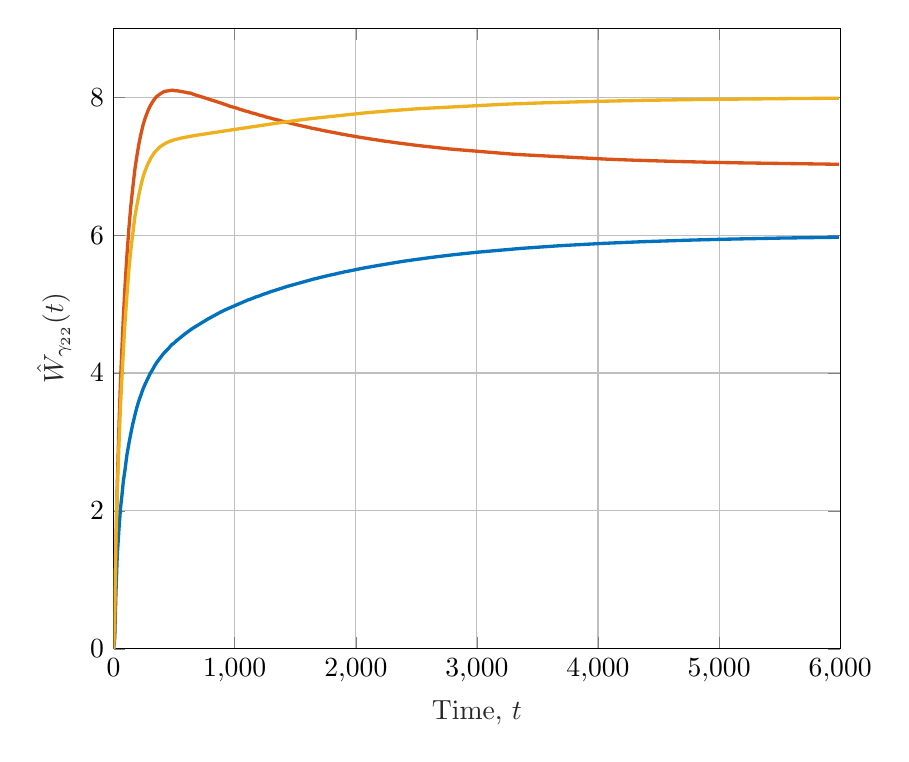
\begin{tikzpicture}

\begin{axis}[%
width=0.761\textwidth,
height=0.65\textwidth,
at={(0\textwidth,0\textwidth)},
scale only axis,
xmin=0,
xmax=6000,
xlabel style={font=\color{white!15!black}},
xlabel={Time, $t$},
ymin=0,
ymax=9,
ylabel style={font=\color{white!15!black}},
ylabel={$\hat{W}_{\gamma_{22}} (t)$},
axis background/.style={fill=white},
xmajorgrids,
ymajorgrids
]
\addplot [color=mycolor1, line width=1.2pt, forget plot]
  table[row sep=crcr]{%
0	0\\
8.82567774673498	0.1570836457513\\
19.0172805425273	0.818044322419155\\
29.8429018432244	1.35210289458792\\
43.2073612132581	1.71986362172902\\
56.5598050272929	2.03486060621981\\
67.4381941604706	2.20656914763276\\
79.6566813477057	2.42592614054138\\
94.2494444992581	2.6016878879982\\
109.745317186334	2.81440251464483\\
125.853275747037	2.9758590483525\\
142.009734557038	3.12529666256341\\
158.358176006041	3.26348820976455\\
174.711371588775	3.38237941780335\\
191.072830577384	3.49570398112155\\
209	3.60279161266317\\
226.168675099905	3.68427968146261\\
242.620196855619	3.76796127469879\\
258.852456575039	3.83374221545728\\
302.51819529059	3.99550653021743\\
313.26064574162	4.02412071247636\\
338.638266648485	4.10381296101696\\
352.896711270768	4.14499861963486\\
410.005138169928	4.27768066400768\\
439.531122822289	4.33266947560242\\
454.191877487838	4.35709478657009\\
469.742592788507	4.39111588107244\\
485.003432151922	4.41723532920696\\
499.195713385834	4.43460080038585\\
514.481507652563	4.46073622647054\\
589.009737285974	4.56723762533329\\
651.525181688713	4.64689580687173\\
778.151535992266	4.78237643538705\\
881.294893168033	4.88095572112707\\
926.071906752755	4.91945265675895\\
1112.1414102175	5.06118343587696\\
1126.41322729571	5.06803676067557\\
1183.966814416	5.10904129172286\\
1198.37007951098	5.11515718380087\\
1241.02402858683	5.1451878286889\\
1255.13578538528	5.15095732104874\\
1297.79156238096	5.17963592284468\\
1326.38749168956	5.19460766953944\\
1427.03325909142	5.25215993775873\\
1655.22948084283	5.36357750738262\\
1683.36182621836	5.3747188180796\\
1697.20603267102	5.38215123130067\\
1724.82559615905	5.3928293355666\\
1780.88227047121	5.41718424552437\\
1810.0097375071	5.42703484546928\\
1853	5.44591548669086\\
1880.96020294399	5.45561849910791\\
1909.94897891313	5.46758891778882\\
1938.36237587037	5.47694507633787\\
2069.08586904938	5.52370510586661\\
2200.17097302751	5.56386915597341\\
2389.65384328071	5.61902254463348\\
2447.64605787809	5.63384566237892\\
2506.04379142415	5.64789792058855\\
2622.4647014881	5.67579350606229\\
2786.40698187097	5.71093192911212\\
2881.00486886656	5.72886555879177\\
3002.67746572809	5.75138596896068\\
3365.08626283721	5.80712491176746\\
3662.03319733834	5.84313063179889\\
3759.23537996154	5.85308071912095\\
4028.04261853622	5.87836922345286\\
4153.02995382097	5.88815853383858\\
4370.10089920308	5.9041287976288\\
4774.95517770591	5.9276622955831\\
5034.17126461824	5.9395261421887\\
5520.36250334343	5.95694066534179\\
5989.14757750197	5.96878202055632\\
};
\addplot [color=mycolor2, line width=1.2pt, forget plot]
  table[row sep=crcr]{%
0	0\\
8.82567774673498	0.25158821070454\\
19.0172805425273	1.41383400143786\\
29.8429018432244	2.378590762567\\
43.2073612132581	3.19259847044668\\
56.5598050272929	3.88894346216966\\
67.4381941604706	4.32248522451391\\
79.6566813477057	4.79733039834355\\
94.2494444992581	5.2664846204907\\
109.745317186334	5.7090833229031\\
125.853275747037	6.09575201384359\\
142.009734557038	6.42414691120302\\
158.358176006041	6.69179963744409\\
174.711371588775	6.94357798065903\\
191.072830577384	7.13944630743208\\
209	7.32688532846623\\
226.168675099905	7.4721906497989\\
242.620196855619	7.5936512669241\\
258.852456575039	7.68784595440866\\
274.37469863266	7.76244585388486\\
289.014607951359	7.8261482436219\\
302.51819529059	7.87577273882107\\
325.049033754998	7.94047093012432\\
338.638266648485	7.97448205801447\\
352.896711270768	8.00563457911448\\
381.438745694973	8.04391217130797\\
410.005138169928	8.07635222300451\\
424.644423402465	8.08475111155076\\
485.003432151922	8.10189287089452\\
499.195713385834	8.09548397264371\\
529.414315658441	8.09131843334035\\
589.009737285974	8.07272041031865\\
619.131785191333	8.060274606235\\
635.086782732727	8.05852321018756\\
667.004864362281	8.03718557333559\\
763.157774875984	7.98399823089676\\
881.294893168033	7.91761304573356\\
940.652533654194	7.88197644507818\\
955.063897009115	7.87123106259969\\
1025.00342172574	7.83675604303789\\
1039	7.82523434923223\\
1068	7.81089060097383\\
1097.49475195213	7.79466709942153\\
1112.1414102175	7.79055014359892\\
1126.41322729571	7.77932678071193\\
1183.966814416	7.75262099773954\\
1198.37007951098	7.74199275832416\\
1241.02402858683	7.72417784492427\\
1255.13578538528	7.71389664350136\\
1297.79156238096	7.69645619609219\\
1311.65627142704	7.68742777826537\\
1369.99410956871	7.66340608686824\\
1384.20268500634	7.6541293263208\\
1427.03325909142	7.63851693026299\\
1501.00486862834	7.60426051182458\\
1571.38614387203	7.5767218320816\\
1599.13444431504	7.5655340764315\\
1613.18400244325	7.5620091321116\\
1627.18460272661	7.55365967535363\\
1697.20603267102	7.53003799532689\\
1724.82559615905	7.51799292047235\\
1853	7.47559544299293\\
1880.96020294399	7.46501015680133\\
1909.94897891313	7.45718863263028\\
1938.36237587037	7.44719864686704\\
2039.94274093853	7.41647831690079\\
2156.37531649316	7.38419587898898\\
2185.81475078068	7.37717681400773\\
2214.88592636115	7.36793194236452\\
2287.73425798115	7.35101972307802\\
2331.02332908133	7.33984945947577\\
2506.04379142415	7.30024997227429\\
2650.85118649742	7.27248998661435\\
2705.03331917403	7.26226728021629\\
2773.07210320797	7.24887273967943\\
3321.92259512344	7.16993596427164\\
4082.60349984987	7.10021924061039\\
4297.25047441858	7.08608212580748\\
4658.39910775497	7.06722285283922\\
4945.9243204362	7.05524068708291\\
5135.85561430633	7.04828757364794\\
5989.14757750197	7.02674272103286\\
};
\addplot [color=mycolor3, line width=1.2pt, forget plot]
  table[row sep=crcr]{%
0	0\\
8.82567774673498	0.590403737484849\\
19.0172805425273	1.61678821500391\\
29.8429018432244	2.30122101063625\\
43.2073612132581	2.93069761381594\\
56.5598050272929	3.51761342093323\\
67.4381941604706	3.89794474444443\\
79.6566813477057	4.30098791259206\\
94.2494444992581	4.74346447475546\\
109.745317186334	5.12403696807178\\
125.853275747037	5.49821970697576\\
142.009734557038	5.78771177079943\\
174.711371588775	6.25858045099994\\
191.072830577384	6.42356373080929\\
209	6.59016107739353\\
226.168675099905	6.72810297041542\\
242.620196855619	6.84152137865385\\
258.852456575039	6.926138599968\\
274.37469863266	6.99560562194165\\
289.014607951359	7.05575078418678\\
313.26064574162	7.13385577692225\\
338.638266648485	7.20125381039452\\
381.438745694973	7.27775805857527\\
424.644423402465	7.32748273194557\\
454.191877487838	7.35310639041109\\
499.195713385834	7.38125830806985\\
558.981417999369	7.40741113709646\\
667.004864362281	7.44350897797085\\
763.157774875984	7.4691309645159\\
1068	7.55019748927589\\
1097.49475195213	7.55674956200983\\
1140.56181414791	7.57005666260829\\
1169.03326575125	7.57649090956875\\
1340.71556330274	7.62152791961944\\
1398.36264972659	7.63624642835748\\
1514.92850683944	7.66386657837029\\
1641.23495399155	7.69123523247981\\
2083.89588192289	7.77346523548294\\
2287.73425798115	7.8036947869814\\
2520.56685863806	7.83320999107764\\
3237.48815018133	7.89821871197455\\
3336.13494846969	7.90470598932552\\
3549	7.91780161251154\\
3957.53264358248	7.93827993124341\\
4399.18760949767	7.95445966519219\\
4802.84642894634	7.96553732634766\\
5504.26751180366	7.97867675704492\\
5989.14757750197	7.98497352195227\\
};
\end{axis}
\end{tikzpicture}%
		%\caption{$\hat{W}_\gamma(t)$)}
	\end{subfigure}
	\caption{ Χρονική εξέλιξη των βαρών $\hat{W}_{\gamma_{21}}(t)$ (αριστερά) και $\hat{W}_{\gamma_{22}(t)}$ (δεξιά) για το πείραμα \ref{subsec:rbf_mimo}}
	\label{fig:mimo_gamma2_weights}
\end{figure}


\section{Πραγματικά Συστήματα}
\label{sec:real_system_experiments}
Σε αυτό το σημείο, είμαστε σε θέση να εφαρμόσουμε το σχήμα αναγνώρισης της Ενότητας \ref{chap:scheme_presentation} σε πραγματικά συστήματα. Για τον σκοπό αυτό, επιλέγονται τα εξής τρία  δοκιμαστικά συστήματα:

\begin{itemize}
	\item ένα απλοποιημένο μοντέλο του φαινόμενου \textit{Wing Rock} το οποίο παρουσιάζεται στα αεροσκάφη τύπου \textit{Delta Wing}. Το σύστημα αυτό πρόκειται για ένα δευτεροβάθμιο σύστημα όπου η $f(x)$ είναι συνάρτηση και των δυο καταστάσεων ενώ η $g(x)$ είναι μια σταθερά.
	
	\item ένα οδηγούμενο ταλαντωτή \textit{Van Der Pol}, το οποίο είναι ένα σύστημα δευτέρου βαθμού. Οι συναρτήσεις $f(x)$ και $g(x)$ είναι συναρτήσεις και των δυο καταστάσεων $x_1$, $x_2$ συνεπώς αυτό το σύστημα δεν εμπίπτει στην κατηγορία συστημάτων \textit{Euler Lagrange} που μελετάμε.
	
	\item ένα βραχίονα δυο βαθμών ελευθερίας. Το σύστημα αυτό είναι σύστημα ΠΕΠΕ και εμπίπτει στην κατηγορία \textit{Euler Lagrange} αφού ο πίνακας αδράνειας είναι συνάρτηση μόνο των θέσεων των αρθρώσεων και όχι των ταχυτήτων.
\end{itemize}


\subsection{Φαινόμενο Wing Rock}
\label{exp:wing_rock}
Το σύστημα που θα μελετήσουμε αποτελεί μια μοντελοποίηση του φαινομένου \textit{Wing Rock}. Το φαινόμενο αυτό αναφέρεται την αστάθεια ανοικτού βρόγχου στην γωνία roll, που παρατηρείται στα αεροπλάνα τύπου \textit{Delta Wing} όταν έχουν μεγάλη \textit{γωνία προσβολής (Angle of Attack)}. Το μοντέλο που θα χρησιμοποιηθεί για αυτό το πείραμα μπορεί να βρεθεί στο βιβλίο~\cite{eugene2013robust}.

Το σύστημα αποτελείται από δυο καταστάσεις, την γωνία roll του αεροσκάφους την οποία συμβολίζουμε με $x_1$ και την αντίστοιχη γωνιακή ταχύτητα την οποία συμβολίζουμε με $x_2$. Έτσι λοιπόν, το σύστημα περιγράφεται από τις εξισώσεις καταστάσεων:
\begin{equation}
\begin{split}
\dot{x}_1 &= x_2 \\
\dot{x}_2 &= 
\underbrace{\theta_1 x_1 + \theta_2 x_2 + (\theta_3 \abs{x_1} 
	+ \theta_4 \abs{x_2})x_2 + \theta_5 x_1^3}_{f(x)} 
+ \underbrace{\theta_6}_{g(x)} u(t)
\end{split}
\label{eq:wing_rock_state_space}
\end{equation}
όπου $u(t)$ είναι η είσοδος ελέγχου και τα $\theta_i$ σταθερές που δίνονται στον παρακάτω πίνακα:
\begin{table}[h]
	\begin{center}
		\begin{tabular}{ c | c | c | c | c | c}
			\hline
			\hline
			$\theta_1$ & $\theta_2$  & $\theta_3$ & $\theta_4$  & $\theta_5$ & $\theta_6$  \\   \hline 
			$-0.018$ & $0.015$  & $-0.062$ & $0.009$ & $0.021$ & $0.75$   \\
			\hline
			\hline
		\end{tabular}
		\caption{Σταθερές $\theta_i$ της εξίσωσης~\eqref{eq:wing_rock_state_space}}
		\label{tab:wing_rock_params}
	\end{center}
\end{table}


	
	\subsubsection{Σχήμα Αναγνώρισης}
	Για την αναγνώριση του παραπάνω συστήματος θα εργαστούμε με τον ίδιο τρόπο που εργαστήκαμε στα πειράματα του προηγούμενο κεφαλαίου, με την διαφορά ότι καθώς η $g(x)$ είναι άγνωστη σταθερά, για την εκτίμηση της θα χρησιμοποιήσουμε μια σταθερά έναντι ενός νευρωνικού δικτύου που θα εισήγαγε περιττή πολυπλοκότητα. Έτσι, σχηματίζουμε τις προσεγγίσεις:
	
	{\begin{wraptable}[16]{r}{0.3\textwidth}
			\centering
			\captionsetup{format=plain}
			\caption{Παράμετροι σχήματος αναγνώρισης για το φαινόμενο \textit{Wing Rock}}
			\begin{tabular}{ l | r }
				\hline\hline
				\text{Parameter} & Value \\ \hline\hline
				$k$             & $30$   \\ \hline
				$\lambda$       & $1 $   \\ \hline
				$\beta_{\varphi} \;\text{(bias)}$     & $1$ \\ \hline
				$\beta_{\varphi} \;\text{(gaussian)}$ & $10$ \\ \hline
				$\beta_{\gamma}$ & $0.3$  \\ \hline
				$\rho_0      $ & $4$  \\ \hline
				$\rho_\infty $ & $0.02$  \\ \hline
				$l           $ & $2$  \\ \hline
				$\textit{ΔΤ} $  & $2$ 	\\ \hline \hline	
			\end{tabular}
			\label{tab:wing_rock_schema_params}
		\end{wraptable}
	\begin{equation*}
	\begin{matrix}
	\hat{\varphi}(x,t)  = \hat{W}_{\varphi}^T(t) Z_\varphi(x) & \text{και} &  
	\end{matrix}\hat{\gamma}(t) = w_{\gamma 0}(t)
	\end{equation*}
	
	Σχετικά με την επιλογή του συνόλου αναγνώρισης, ορίζουμε το εύρος της γωνίας $x_1$ ώς το σύνολο $[-\frac{\pi}{4},\frac{\pi}{4}]$, το οποίο φαίνεται λογική τιμή δεδομένου ότι πρόκειται για την γωνία \textit{roll} ενός αεροσκάφους. Αντίθετα, για το σύνολο τιμών δεν γνωρίζουμε ποιο θεωρείται ένα αποδεκτό εύρος και κατά συνέπεια επιλέγεται και εδώ το σύνολο $[-\frac{\pi}{4},\frac{\pi}{4}]$ για λόγους συμμετρίας του συνόλου αναγνώρισης. Έτσι, το σύνολο $\Omega_x$ επιλέγεται ως:
	\begin{equation*}
	\Omega_x = \bmqty{-\frac{\pi}{4},\frac{\pi}{4}} \times \bmqty{-\frac{\pi}{4},\frac{\pi}{4}}
	\end{equation*}
	
	%Τέλος, σημειώνουμε πως το προσπαθούμε να αναγνωρίσουμε το σύστημα για εύρος γωνιών $x_1 \in [-\frac{\pi}{4},\frac{\pi}{4}]$ το οποίο φαίνεται λογική τιμή δεδομένου ότι πρόκειται για την γωνία roll ενός αεροσκάφους. Για το εύρος ταχυτήτων αντίθετα, δεν γνωρίζουμε ποιο θα μπορούσε να είναι ένα καλό σύνολο τιμών και συνεπώς επιλέγεται πάλι το σύνολο \\ $[-\frac{\pi}{4},\frac{\pi}{4}]$ χάριν συμμετρίας του συνόλου αναγνώρισης. Έτσι λοιπόν, το σύνολο αναγνώρισης ορίζεται ως το:
	

	Τα κέντρα του νευρωνικού δικτύου RBF για την αναγνώριση της $\varphi(x)$ επιλέγονται ως ένα πλέγμα που καλύπτει ομοιόμορφα το $\Omega_x$ και αποτελείται από $225$ κέντρα. Τα σημεία του πλέγματος δίνονται παρακάτω:
	\begin{equation*}
	C = \begin{Bmatrix}
	0 \pm \frac{\pi }{28} k, \quad  k \in [0,1,...,7]
	\end{Bmatrix} \times
	\begin{Bmatrix}
	0 \pm  \frac{\pi }{28} k, \quad  k \in [0,1,...,7]
	\end{Bmatrix}
	\end{equation*}
		
	}
	
	Τέλος, χρησιμοποιούμε τους νόμους ελέγχου και την μεθοδολογία σχεδίασης που παρουσιάζεται στην Υποενότητα \ref{subsec:CL_design}, με τις σχεδιαστικές παραμέτρους να δίνονται στον Πίνακα \ref{tab:wing_rock_schema_params}.
	
	\begin{figure}
		\begin{subfigure}{0.5\textwidth}
			% This file was created by matlab2tikz.
%
\definecolor{mycolor1}{rgb}{0.00000,0.44700,0.74100}%
\definecolor{mycolor2}{rgb}{0.85000,0.32500,0.09800}%
\definecolor{mycolor3}{rgb}{0.92900,0.69400,0.12500}%
\definecolor{mycolor4}{rgb}{0.49400,0.18400,0.55600}%
\definecolor{mycolor5}{rgb}{0.46600,0.67400,0.18800}%
%
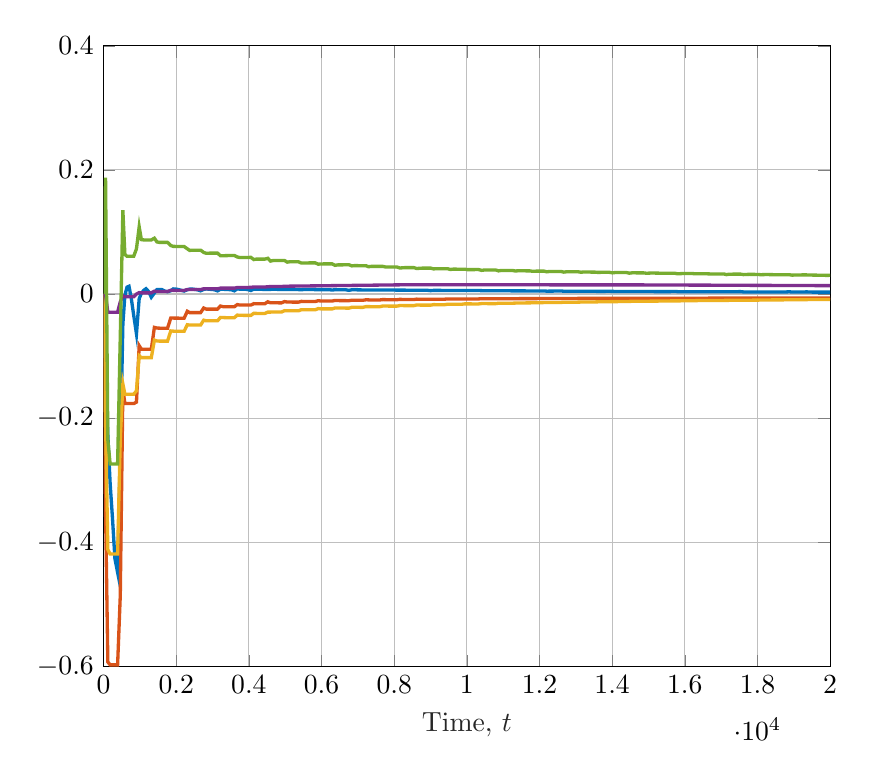
\begin{tikzpicture}

\begin{axis}[%
width=0.761\textwidth,
height=0.65\textwidth,
at={(0\textwidth,0\textwidth)},
scale only axis,
xmin=0,
xmax=20000,
xlabel style={font=\color{white!15!black}},
xlabel={Time, $t$},
ymin=-0.6,
ymax=0.4,
axis background/.style={fill=white},
xmajorgrids,
ymajorgrids
]
\addplot [color=mycolor1, line width=1.2pt, forget plot]
  table[row sep=crcr]{%
0	0\\
55.0635253448527	-0.111327616348717\\
117.740081790336	-0.227057185275044\\
181.042940623629	-0.305215220734681\\
244.250085194657	-0.359955549614824\\
313.054868586372	-0.426725083972997\\
386.450308124524	-0.44840981609741\\
460.383685113178	-0.259586407806637\\
531.534000841482	-0.0483010376156017\\
586.876434306501	-0.00211631864294759\\
645.426620820937	0.0110567115625599\\
699.905954868838	0.0124914947955403\\
759.399194476926	-0.00554637790628476\\
829.61712724575	-0.0342360495124012\\
905.897855748619	-0.0640813034769963\\
980.540087423618	-0.00743184722887236\\
1040.27152598924	0.00104779925459297\\
1104.0820065868	0.00580151737449341\\
1168.46786182063	0.00860434323112713\\
1236.83171231105	0.00426037030774751\\
1314.58935505555	-0.00509485830843914\\
1467.74645415656	0.00710135736517259\\
1534.53957052394	0.00734918484158698\\
1607.58066893003	0.00709908990756958\\
1681.63618586665	0.00485618435413926\\
1760.4341202368	0.00373665739607532\\
1850.02260818859	0.00524391550425207\\
1917.64555705278	0.00826778653208748\\
1984.09249044073	0.00803299202743801\\
2059.20935922616	0.0072444991710654\\
2216.98293982433	0.00481697695795447\\
2305.66755278661	0.00686685453547398\\
2370.22322008605	0.00788398331133067\\
2435.86511830268	0.00805100743309595\\
2584.28817894359	0.00691095506408601\\
2671.13162017401	0.00523384624830214\\
2756.71927630613	0.00742024392820895\\
2826	0.00817298458423465\\
3050.41701689437	0.00699519003683235\\
3136.70760283471	0.00508106759662041\\
3219.5727006804	0.00785717079634196\\
3514.34657875465	0.00698361784452572\\
3600.21579198656	0.00519410243214224\\
3681.25320671459	0.00830130709437071\\
3748.64527367475	0.00785187959627365\\
3897.48908539172	0.00767479325804743\\
3970.29187849578	0.00726607079559471\\
4055.50048240303	0.00564683853372117\\
4135.46502812101	0.00792456411363673\\
4520	0.00735305973284994\\
4669.81735750407	0.00770372348051751\\
5056.12636357825	0.00721602849444025\\
5202.16848206385	0.00738824242580449\\
5364.06769665301	0.00716140650911257\\
5444.95739148318	0.00692508929569158\\
5519.2583009311	0.00729002287334879\\
5979.24208841819	0.00708062022022204\\
6208.67000126774	0.00697327004309045\\
6295.53850735944	0.00649459417763865\\
6369.48363763807	0.00689943079487421\\
6668.18785387962	0.00680948685112526\\
6755.76518661901	0.0059683458021027\\
6835.29388964037	0.00689221698121401\\
7225.80174911133	0.00652663234359352\\
7687.76170848325	0.00645904471821268\\
7912.75343347144	0.00640728018333903\\
8916.31364587013	0.00600212841527537\\
9004.02870191402	0.00544263262054301\\
9084	0.00590577570619644\\
9773.91352726302	0.00569506639658357\\
10323.8781079361	0.00564874269912252\\
10476.9387704231	0.00529994742828421\\
11098.5807061446	0.00518095235020155\\
12033.646375335	0.00492296785887447\\
12117.4962904375	0.00495782330108341\\
12203.8315017742	0.00459997235520859\\
12591.3251568522	0.004914778546663\\
12669.3504107277	0.00453694765747059\\
12974.9394279261	0.00461389014890301\\
13139.1370080632	0.00442990028022905\\
13444.5323880791	0.00456865133674\\
13610.417849542	0.0042485904705245\\
13920.4294907932	0.00439163934788667\\
14076.5842448811	0.00419346697526635\\
14620.5342958314	0.00413027086688089\\
15335.8016951617	0.00387638298707316\\
15640	0.00394894914279575\\
15724.8865507524	0.00421883538001566\\
15809.1310307535	0.00378158692547004\\
16588.6759576406	0.00378028740306036\\
16898.5460594743	0.00365934499859577\\
17536.8328764996	0.00384728896824527\\
17616.1212574965	0.00338014719091007\\
18010.1784161452	0.00334064483467955\\
18786.078783337	0.00334309691243106\\
18872.5229560096	0.00368346412142273\\
18958.2909640011	0.00319129783747485\\
19262.1258487664	0.0032793536738609\\
19349.5963535027	0.00350224488283857\\
19502.5304239961	0.00312831144401571\\
20046.6532646761	0.00311009458164335\\
};
\addplot [color=mycolor2, line width=1.2pt, forget plot]
  table[row sep=crcr]{%
0	0\\
55.0635253448527	-0.34822442845325\\
117.740081790336	-0.592954861935141\\
181.042940623629	-0.597584565839497\\
386.450308124524	-0.597584565839497\\
460.383685113178	-0.485454028046661\\
531.534000841482	-0.152763029371272\\
586.876434306501	-0.17651929063868\\
829.61712724575	-0.17651929063868\\
905.897855748619	-0.174170668360603\\
980.540087423618	-0.083290227343241\\
1040.27152598924	-0.0888840755105775\\
1314.58935505555	-0.0888840755105775\\
1399.12949507979	-0.0538108296459541\\
1467.74645415656	-0.0548112515025423\\
1607.58066893003	-0.0551499431603588\\
1760.4341202368	-0.0551499431603588\\
1850.02260818859	-0.0386989240905677\\
2216.98293982433	-0.0389828871266218\\
2305.66755278661	-0.0277521890566277\\
2370.22322008605	-0.0299086707273091\\
2671.13162017401	-0.0299086707273091\\
2756.71927630613	-0.0225412417785265\\
2826	-0.0242791273158218\\
3136.70760283471	-0.0242791273158218\\
3219.5727006804	-0.0193452008134045\\
3293.90731473371	-0.0204324106089189\\
3600.21579198656	-0.0204324106089189\\
3681.25320671459	-0.0169818424437835\\
3748.64527367475	-0.0177185684369761\\
4055.50048240303	-0.0177652505881269\\
4135.46502812101	-0.0154955943580717\\
4283.28440167238	-0.015742198251246\\
4436.43256239406	-0.015742198251246\\
4520	-0.0125214313738979\\
4593.4245485769	-0.0140963704325259\\
4896.46780104089	-0.0142214670195244\\
4982.82944944579	-0.0121354093462287\\
5056.12636357825	-0.0129458818155399\\
5364.06769665301	-0.0130215974641033\\
5444.95739148318	-0.0118637951673009\\
5668.31306972509	-0.0121041933343804\\
5825.86201886375	-0.0121041933343804\\
5908.47551219729	-0.0106926813605241\\
5979.24208841819	-0.0112768540348043\\
6295.53850735944	-0.0112768540348043\\
6369.48363763807	-0.0102910949099169\\
6516.66382830188	-0.0106414697984292\\
6755.76518661901	-0.0106912400624424\\
6835.29388964037	-0.00996660844248254\\
7054.43731724382	-0.0100859589147149\\
7136.50953682102	-0.0100859589147149\\
7225.80174911133	-0.00924848205977469\\
7371.68740853718	-0.00961823428224307\\
7600.19755424963	-0.00961823428224307\\
7687.76170848325	-0.00891430748743005\\
7834.31187342255	-0.00921027129879803\\
8070.56855446964	-0.00921027129879803\\
8156	-0.00855444167973474\\
8303.09295371648	-0.00886463633287349\\
8540.17542978077	-0.00886463633287349\\
8615.40692040867	-0.00823019254312385\\
8763.30760063444	-0.00854136692578322\\
9386.67096525965	-0.00830071248492459\\
9474.26053180134	-0.00786477468864177\\
9622.26226319045	-0.00809865669725696\\
10323.8781079361	-0.00787895317989751\\
10407.8568707344	-0.00745718624602887\\
10555.5400869796	-0.00764756158605451\\
12117.4962904375	-0.00729841815700638\\
12273.9765643506	-0.00715959479930461\\
13920.4294907932	-0.00692131208415958\\
14076.5842448811	-0.00685231750685489\\
17536.8328764996	-0.00657348532331525\\
17766.69078949	-0.00654028891949565\\
20046.6532646761	-0.00645622043884941\\
};
\addplot [color=mycolor3, line width=1.2pt, forget plot]
  table[row sep=crcr]{%
0	0\\
55.0635253448527	-0.205679843857069\\
117.740081790336	-0.411930654143362\\
181.042940623629	-0.41904516971772\\
386.450308124524	-0.41904516971772\\
460.383685113178	-0.233264982496621\\
531.534000841482	-0.144796278895228\\
586.876434306501	-0.161454162625887\\
829.61712724575	-0.161454162625887\\
905.897855748619	-0.156032962309837\\
980.540087423618	-0.099331644429185\\
1040.27152598924	-0.102502948382607\\
1314.58935505555	-0.102502948382607\\
1399.12949507979	-0.07427079667832\\
1467.74645415656	-0.0754879086161964\\
1534.53957052394	-0.0758961013198132\\
1760.4341202368	-0.0758961013198132\\
1850.02260818859	-0.0594459183812432\\
1984.09249044073	-0.0600979831033328\\
2216.98293982433	-0.0600979831033328\\
2305.66755278661	-0.0494839998937096\\
2370.22322008605	-0.0499820851619006\\
2671.13162017401	-0.0499820851619006\\
2756.71927630613	-0.0421507586252119\\
2826	-0.0431077782523062\\
3136.70760283471	-0.0431077782523062\\
3219.5727006804	-0.0376964696297364\\
3363.53693900999	-0.0380865302940947\\
3600.21579198656	-0.0380865302940947\\
3681.25320671459	-0.0339862964829081\\
3819.6660808091	-0.0343202193616889\\
4055.50048240303	-0.0344094231768395\\
4135.46502812101	-0.0310601476412558\\
4283.28440167238	-0.0313745648636541\\
4436.43256239406	-0.0313745648636541\\
4520	-0.0291452687160927\\
4669.81735750407	-0.029052846297418\\
4896.46780104089	-0.029052846297418\\
4982.82944944579	-0.026796665351867\\
5202.16848206385	-0.0270699556822365\\
5364.06769665301	-0.0270699556822365\\
5444.95739148318	-0.0252208284182416\\
5825.86201886375	-0.0253748143513803\\
5908.47551219729	-0.0234314488661767\\
5979.24208841819	-0.0238840589881875\\
6295.53850735944	-0.0238840589881875\\
6369.48363763807	-0.0224140189820901\\
6595.61809127813	-0.02258617699772\\
6755.76518661901	-0.0227380013093352\\
6835.29388964037	-0.0212960154822213\\
7054.43731724382	-0.0214402831734333\\
7136.50953682102	-0.0214402831734333\\
7225.80174911133	-0.0202379034635669\\
7443.0503964347	-0.0204442265494436\\
7600.19755424963	-0.0204442265494436\\
7687.76170848325	-0.0192640471832419\\
7912.75343347144	-0.0195098912154208\\
8070.56855446964	-0.0195098912154208\\
8156	-0.0185617856623139\\
8374.30005898322	-0.0186843196715927\\
8540.17542978077	-0.0186843196715927\\
8615.40692040867	-0.0176634866147651\\
8763.30760063444	-0.0178996024696971\\
9004.02870191402	-0.0178996024696971\\
9084	-0.0171056734543527\\
9386.67096525965	-0.017198567646119\\
9474.26053180134	-0.0163895020341442\\
9773.91352726302	-0.0165378549791058\\
9854.61610596025	-0.0165378549791058\\
9938.63601013589	-0.0158607975863561\\
10323.8781079361	-0.015960391745466\\
10407.8568707344	-0.0152923423702305\\
10626.7173810016	-0.015436971836607\\
10795.5535173767	-0.015436971836607\\
10872	-0.0148600757311215\\
11177.7614022263	-0.0149154201499186\\
11409.3386447832	-0.0144306206348119\\
11731.5043077365	-0.0142318244688795\\
11880.8642507953	-0.0140077061441843\\
12203.8315017742	-0.0136821039232018\\
12425.5231595294	-0.0135618445274304\\
12591.3251568522	-0.0135618445274304\\
12669.3504107277	-0.0131448727333918\\
13059.3880078797	-0.013089945907268\\
13209.0841539908	-0.0127856815815903\\
13533.3780041553	-0.0127198887821578\\
13682.6489695844	-0.012412135311024\\
14394.436803427	-0.0120512692883494\\
14548.5973743014	-0.011716190369043\\
15335.8016951617	-0.0113354960158176\\
15485.4954404219	-0.0111212186820921\\
16200.1626173772	-0.0108353136893129\\
16354.2752437497	-0.0105584904049465\\
17150.2190837534	-0.0102455819433089\\
17298	-0.0100372359338508\\
18010.1784161452	-0.00982154345911113\\
18162.2945964616	-0.00953526221928769\\
18872.5229560096	-0.00930377876647981\\
19106.5714079608	-0.00909114562091418\\
19825.4380872084	-0.0087212624384847\\
20046.6532646761	-0.0086547887949564\\
};
\addplot [color=mycolor4, line width=1.2pt, forget plot]
  table[row sep=crcr]{%
0	0\\
55.0635253448527	-0.00103598312489339\\
117.740081790336	-0.0294017299784173\\
386.450308124524	-0.0294017299784173\\
460.383685113178	-0.0125510160942213\\
531.534000841482	-0.0029616528081533\\
586.876434306501	-0.00438166035382892\\
829.61712724575	-0.00438166035382892\\
905.897855748619	5.73568831896409e-06\\
980.540087423618	0.00227788045594934\\
1040.27152598924	0.00191944999096449\\
1314.58935505555	0.00191944999096449\\
1399.12949507979	0.00460946158636943\\
1467.74645415656	0.00412041013987618\\
1760.4341202368	0.00412041013987618\\
1850.02260818859	0.00603452812720207\\
1984.09249044073	0.00578764490637695\\
2216.98293982433	0.00578764490637695\\
2305.66755278661	0.00731285406072857\\
2510.1479600702	0.00719425602437695\\
2671.13162017401	0.00719425602437695\\
2756.71927630613	0.00847548907768214\\
3136.70760283471	0.00843701675330522\\
3219.5727006804	0.00951403375438531\\
3600.21579198656	0.00952056769892806\\
3681.25320671459	0.0104861094296211\\
3970.29187849578	0.0105010621809924\\
4135.46502812101	0.0112942678206309\\
4436.43256239406	0.0113157832784054\\
4593.4245485769	0.0120779975804908\\
4896.46780104089	0.0120771551810321\\
4982.82944944579	0.0126006756690913\\
8374.30005898322	0.0149777675542282\\
14864.0356074504	0.0147142346140754\\
15092.2801661918	0.0145699866043287\\
16676.026609688	0.0143310865314561\\
16898.5460594743	0.01418213013676\\
18397.0989144324	0.013898093617172\\
18786.078783337	0.0137912925019918\\
20046.6532646761	0.0135017392603913\\
};
\addplot [color=mycolor5, line width=1.2pt, forget plot]
  table[row sep=crcr]{%
0	0\\
55.0635253448527	0.18764544660371\\
117.740081790336	-0.235250941779668\\
181.042940623629	-0.273792253403371\\
386.450308124524	-0.273792253403371\\
460.383685113178	-0.0673506387720408\\
531.534000841482	0.135023867984273\\
586.876434306501	0.0638085971950204\\
645.426620820937	0.0608398885051429\\
829.61712724575	0.0608398885051429\\
905.897855748619	0.0728481677724631\\
980.540087423618	0.108415765284008\\
1040.27152598924	0.0876878316194052\\
1104.0820065868	0.0872158874044544\\
1314.58935505555	0.0872158874044544\\
1399.12949507979	0.0899676564295078\\
1467.74645415656	0.0840261472294515\\
1534.53957052394	0.0832485818100395\\
1760.4341202368	0.0832485818100395\\
1850.02260818859	0.0781858815425949\\
1917.64555705278	0.0768392799618596\\
2059.20935922616	0.0765710519262939\\
2216.98293982433	0.0765710519262939\\
2370.22322008605	0.0702353737760859\\
2435.86511830268	0.0706886684747587\\
2671.13162017401	0.0706886684747587\\
2756.71927630613	0.0670756588115182\\
2826	0.0656981007305149\\
2969.62424814163	0.0659681483848544\\
3136.70760283471	0.0659681483848544\\
3219.5727006804	0.0616591955586046\\
3514.34657875465	0.0621019700047327\\
3600.21579198656	0.0621019700047327\\
3681.25320671459	0.0597221461684967\\
3748.64527367475	0.0587741727867979\\
4055.50048240303	0.0590561009121302\\
4135.46502812101	0.0555522925023979\\
4204.22739903653	0.0562478902793373\\
4436.43256239406	0.0562478902793373\\
4520	0.0575511591814575\\
4593.4245485769	0.0531175648648059\\
4669.81735750407	0.0539682121416263\\
4982.82944944579	0.0539677676242718\\
5056.12636357825	0.0514287812184193\\
5129.47747121608	0.0519984015991213\\
5364.06769665301	0.0519984015991213\\
5444.95739148318	0.0499194087497017\\
5668.31306972509	0.0501790661437553\\
5825.86201886375	0.0501790661437553\\
5908.47551219729	0.0481598520891566\\
6056.76918588414	0.0485833659004129\\
6295.53850735944	0.0485833659004129\\
6369.48363763807	0.0462575658202695\\
6445.35645159662	0.0469507293419156\\
6668.18785387962	0.0470947471549152\\
6755.76518661901	0.047171339741908\\
6835.29388964037	0.0453456401082803\\
6905.32093425183	0.0457921116467332\\
7225.80174911133	0.0455847096782236\\
7295.5408346779	0.0439338816649979\\
7371.68740853718	0.0446139430205221\\
7687.76170848325	0.044584536968614\\
7764.01760958197	0.0435664439792163\\
8070.56855446964	0.0435583412108826\\
8156	0.0419760870172468\\
8303.09295371648	0.0425752248702338\\
8540.17542978077	0.0425752248702338\\
8615.40692040867	0.04116656959377\\
8763.30760063444	0.041704953302542\\
9004.02870191402	0.0417680961254518\\
9084	0.0404648716066731\\
9153.50332907491	0.0408554662826646\\
9474.26053180134	0.0407662103389157\\
9545.61481232983	0.0395273570684367\\
9622.26226319045	0.0401065895457577\\
9938.63601013589	0.0400327892093628\\
10015.1315674989	0.0393826332328899\\
10323.8781079361	0.0393989300682733\\
10407.8568707344	0.0381763265868358\\
10476.9387704231	0.0386376163878595\\
10795.5535173767	0.0387215664813993\\
10872	0.0373388080588484\\
10948.1095443202	0.0380515450451639\\
11261.5957586179	0.0379081956562004\\
11338.8420099892	0.0370842354750494\\
11409.3386447832	0.0375216617758269\\
11731.5043077365	0.0372986869115266\\
11806.3244445937	0.0366608625772642\\
11956.8315484861	0.0369725374912377\\
12117.4962904375	0.0369725374912377\\
12203.8315017742	0.0357996860257117\\
12273.9765643506	0.0363584859987895\\
12591.3251568522	0.0364555509695492\\
12669.3504107277	0.0353030511359975\\
12746.2895433806	0.0359062753013859\\
13059.3880078797	0.035922801187553\\
13139.1370080632	0.0351178956079821\\
13209.0841539908	0.0355196188065747\\
13533.3780041553	0.0352642003235815\\
13610.417849542	0.034861380358052\\
13760.4543881899	0.0350683561446203\\
13920.4294907932	0.0350683561446203\\
14005.8405748995	0.034105041744624\\
14076.5842448811	0.0345903871966584\\
14394.436803427	0.0346551466136589\\
14471.8755778049	0.0335902507176797\\
14548.5973743014	0.034197461536678\\
14864.0356074504	0.0340748554081074\\
14942.2503586814	0.0335255466561648\\
15092.2801661918	0.033850365653052\\
15335.8016951617	0.0335827618837357\\
15564.4176460536	0.0334518195413693\\
15724.8865507524	0.0334518195413693\\
15809.1310307535	0.0326005917304428\\
15959.2342436125	0.0331170744684641\\
16200.1626173772	0.0331170744684641\\
16281.7132291712	0.0326012781079044\\
16505.5730051234	0.0327759211213561\\
16676.026609688	0.0324614286400902\\
16749.2312478122	0.0321485281128844\\
16898.5460594743	0.0324207007251971\\
17065.5367997623	0.0324207007251971\\
17150.2190837534	0.0312826175577356\\
17222.8406776725	0.0320078559379908\\
17536.8328764996	0.0320747322330135\\
17616.1212574965	0.0313041381778021\\
17766.69078949	0.0317459068064636\\
18010.1784161452	0.0315712976735085\\
18090.2964904092	0.0311450284498278\\
18238.507709027	0.0314267411049514\\
18484	0.0311535768960312\\
18631.9560934274	0.0311303569942538\\
18872.5229560096	0.0311303569942538\\
18958.2909640011	0.0303919920988847\\
19030.0099239281	0.0307939691192587\\
19349.5963535027	0.0308371202372655\\
19502.5304239961	0.0305391219517333\\
19825.4380872084	0.0302370888384758\\
19897.8033362841	0.030009604877705\\
20046.6532646761	0.0302799955388764\\
};
\end{axis}
\end{tikzpicture}%
			%\caption{$\hat{W}_\varphi(t)$}
		\end{subfigure}
		\begin{subfigure}{0.5\textwidth}
			% This file was created by matlab2tikz.
%
\definecolor{mycolor1}{rgb}{0.00000,0.44700,0.74100}%
%
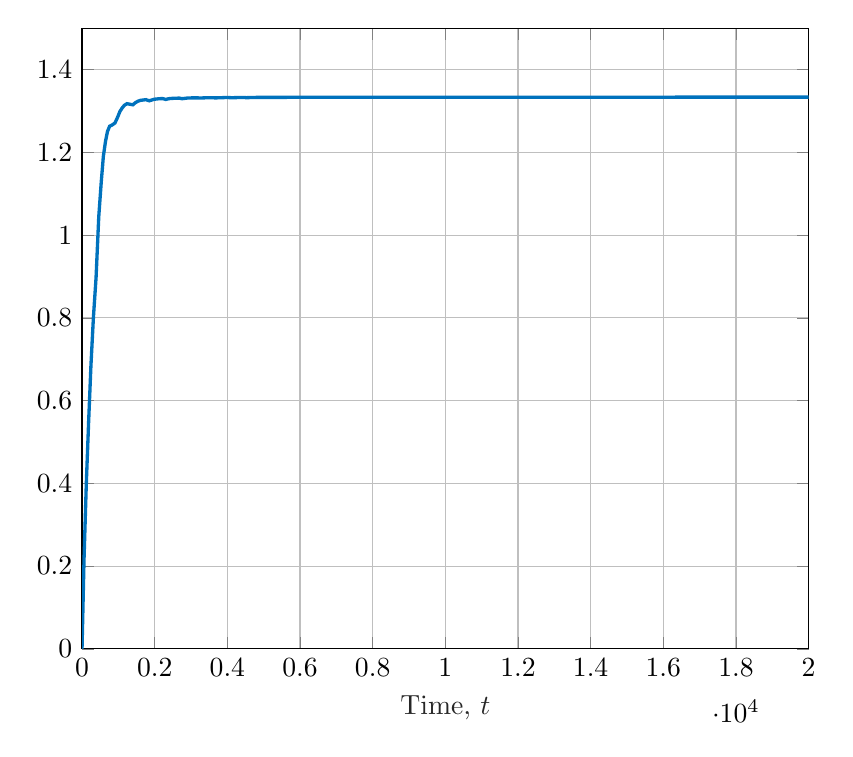
\begin{tikzpicture}

\begin{axis}[%
width=0.761\textwidth,
height=0.65\textwidth,
at={(0\textwidth,0\textwidth)},
scale only axis,
xmin=0,
xmax=20000,
xlabel style={font=\color{white!15!black}},
xlabel={Time, $t$},
ymin=0,
ymax=1.5,
axis background/.style={fill=white},
xmajorgrids,
ymajorgrids
]
\addplot [color=mycolor1, line width=1.2pt, forget plot]
  table[row sep=crcr]{%
0	0\\
55.0635253448527	0.216731584900117\\
117.740081790336	0.399446685289149\\
181.042940623629	0.547557095655065\\
244.250085194657	0.683246308086382\\
313.054868586372	0.800880339695141\\
386.450308124524	0.897745819194824\\
460.383685113178	1.04451681849605\\
531.534000841482	1.13143371897604\\
586.876434306501	1.19007260575381\\
645.426620820937	1.22628574023474\\
699.905954868838	1.25026074998095\\
759.399194476926	1.26317161205588\\
829.61712724575	1.26621924603387\\
905.897855748619	1.27083389907057\\
980.540087423618	1.28512646258969\\
1040.27152598924	1.29834308311183\\
1104.0820065868	1.30716906036469\\
1168.46786182063	1.313888388544\\
1236.83171231105	1.31758629703836\\
1399.12949507979	1.31490852757997\\
1467.74645415656	1.31999305491991\\
1534.53957052394	1.32335991920263\\
1607.58066893003	1.32566610894719\\
1760.4341202368	1.3273330294578\\
1850.02260818859	1.32454752994454\\
1984.09249044073	1.32831112435451\\
2132.77376874798	1.32965520660218\\
2216.98293982433	1.32995986245805\\
2305.66755278661	1.32785896859423\\
2370.22322008605	1.32935564930085\\
2435.86511830268	1.33024155751627\\
2671.13162017401	1.33107395498882\\
2756.71927630613	1.32964255130719\\
2899.52563137137	1.3311913542093\\
3050.41701689437	1.33170386421989\\
3293.90731473371	1.33146749270236\\
3514.34657875465	1.33213541047007\\
3681.25320671459	1.3315765823063\\
3970.29187849578	1.33250803089322\\
4135.46502812101	1.33203233695895\\
4436.43256239406	1.33272953740743\\
4520	1.33211301437768\\
4820.293060478	1.33285148674258\\
5743.70337050336	1.33294239259703\\
7136.50953682102	1.33314651799446\\
7295.5408346779	1.33308620134267\\
20046.6532646761	1.3334801533274\\
};
\end{axis}
\end{tikzpicture}%
			%\caption{$\hat{W}_\gamma(t)$)}
		\end{subfigure}
		\caption{ Χρονική εξέλιξη των βαρών $\hat{W}_\varphi(t)$ (αριστερά) και της σταθεράς $\hat{w}_{\gamma 0}(t)$ (δεξιά) συναρτήσει του χρόνου.}
		\label{fig:wing_rock_weights}
	\end{figure}

\begin{figure}
	\begin{subfigure}{0.5\textwidth}
		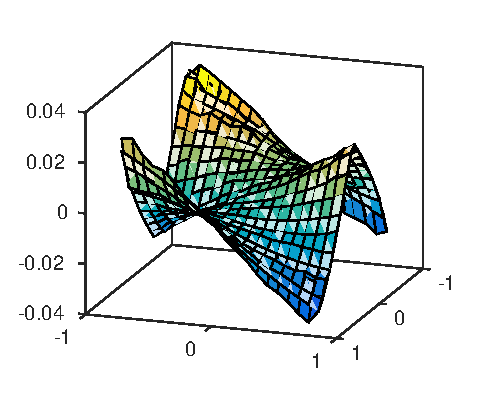
\includegraphics{plots/experiments/wing_rock/f_approx_surf.eps}
		%\caption{$\hat{W}_\varphi(t)$}
	\end{subfigure}
	\begin{subfigure}{0.5\textwidth}
		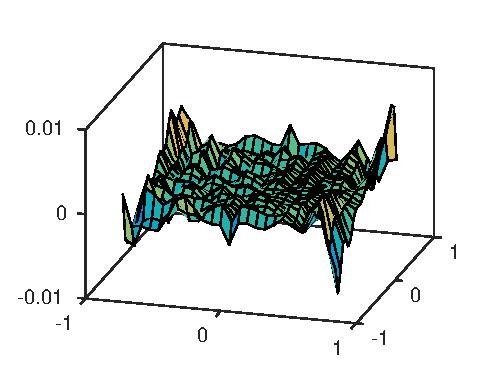
\includegraphics{plots/experiments/wing_rock/f_approx_error.eps}
		%\caption{$\hat{W}_\gamma(t)$)}
	\end{subfigure}
	\caption{Προσέγγιση της συνάρτησης $\varphi(x)$ (αριστερά) και το σφάλμα $\tilde{\varphi}(x)$ (δεξιά) στο πείραμα \textit{Wing Rock}.}
	\label{fig:wing_rock_phi_approximation}
\end{figure}

\subsubsection{Αποτελέσματα}
Μετά από προσομοίωση του συστήματος κλειστού βρόγχου για 50 περιόδους, στο Σχήμα \ref{fig:wing_rock_weights} παρουσιάζεται η χρονική εξέλιξη κάποιων βαρών $\hat{w}_{\varphi i}$ και της σταθεράς $\hat{w}_{\gamma 0}(t)$ συναρτήσει του χρόνου. Από το σχήμα είναι προφανές πως ο χρόνος εκπαίδευσης ήταν αρκετός για να συγκλίνουν τα βάρη του νευρωνικού δικτύου καθώς και η σταθερά  $\hat{w}_{\gamma 0}(t)$ που χρησιμοποιείται για την εκτίμηση της $\gamma(x)$.

Στο Σχήμα \ref{fig:wing_rock_phi_approximation} παρουσιάζεται η προσέγγιση της συνάρτησης $\hat{\varphi}(x)$ καθώς και το σφάλμα $\tilde{\varphi}(x)$. Όπως φαίνεται από τις δυο αυτές γραφικές παραστάσεις, το αποτέλεσμα της διαδικασίας αναγνώρισης της $\varphi(x)$ είναι πολύ ικανοποιητικό. Τέλος, παραθέτουμε έναν πίνακα (Πίνακας \ref{tab:stat_of_function_wing_rock}) με κάποια χαρακτηριστικά του σφάλματος προσέγγισης καθώς και της συνάρτησης $\varphi(x)$ εντός του συνόλου $\Omega_x$ ,έτσι ώστε να διευκολύνουμε την εξαγωγή συμπερασμάτων για την ποιότητα της προσέγγισης.

\begin{table}
	\centering
	\begin{tabular}{  c | c | c | c | c | c }
		& $\min_{x \in \Omega_x}$ & $\max_{x \in \Omega_x}$ & Εύρος Τιμών & $\max(\abs{\tilde{\varphi}(x)})$ & Σχετικό Σφάλμα \\ \hline
		$\varphi(x)$ & $-0.0325$ & $0.0332$ & $0.0657$ & $0.0084$ & $12.79\%$ \\
	\end{tabular}
	\caption{Στατιστικά στοιχειά προσεγγίσεων για το φαινόμενο  \textit{Wing Rock}}
	\label{tab:stat_of_function_wing_rock}
\end{table}

Όπως μπορούμε να δούμε και από τον Πίνακα \ref{tab:stat_of_function_wing_rock}, το μέγιστο ποσοστιαίο ή σχετικό  σφάλμα προσέγγισης εντός του $\Omega_x$ είναι $12.79\%$, γεγονός που επιβεβαιώνει πως τα αποτελέσματα είναι πολύ ικανοποιητικά.

Σχετικά με την ποιότητα προσέγγισης της $\gamma(x)$ η πραγματική τιμή της είναι ίση με $1/\theta_6 = 1.3333$ ενώ το βάθος $w_{\gamma 0}(t)$ συγκλίνει στην τιμή $1.3335$, που σημαίνει ότι και σε αυτή την περίπτωση το σχήμα αναγνωρίζει επιτυχώς την άγνωστη συνάρτηση.


\subsection{Ταλαντωτής \textit{Van der Pol}}
\label{exp:vdp}
Το δεύτερο πραγματικό σύστημα που θα μελετήσουμε είναι ένας οδηγούμενος ταλαντωτής \textit{Van der Pol}, το οποίο είναι ένα αρκετά κλασσικό σύστημα στην βιβλιογραφία του αυτομάτου ελέγχου. 

Το σύστημα αυτό είναι ένα μη-γραμμικό σύστημα δευτέρου βαθμού και περιγράφεται από τις εξισώσεις
\begin{equation}
\begin{split}
\dot{x}_1 &= x_2 \\
\dot{x}_2 &= \mu (1-x_1^2)x_2 - x_1 + 1+x_1^2+x_2^2)u(t)
\end{split}
\end{equation}
όπου $\mu$ θετική σταθερά. Στο πείραμα μας θεωρούμε πως $\mu = 1$. Όπως μπορούμε να δούμε η $g(x)$ σε αυτή την περίπτωση είναι συνάρτηση και των δυο καταστάσεων, συνεπώς το σύστημα δεν είναι τύπου \textit{Euler Lagrange}.


{\begin{wraptable}[16]{r}{0.3\textwidth}
		\centering
		\captionsetup{format=plain}
		\caption{Παράμετροι σχήματος αναγνώρισης για τον ταλαντωτή \textit{Van Der Pol}}
		\label{tab:vdp_schema_params}
		\begin{tabular}{ l | c }
			\hline\hline
			\text{Parameter} & Value \\ \hline\hline
			$k$             & $30$   \\ \hline
			$\lambda$       & $1 $   \\ \hline
			$\beta_{\varphi} \;\text{(bias)}$     & $10$ \\ \hline
			$\beta_{\varphi} \;\text{(gaussian)}$ & $50$ \\ \hline
			$\beta_{\gamma} \;\text{(bias)}$     & $5$ \\ \hline
			$\beta_{\gamma} \;\text{(gaussian)}$ & $20$ \\ \hline
			$\rho_0      $ & $4$  \\ \hline
			$\rho_\infty $ & $0.02$  \\ \hline
			$l           $ & $2$  \\ \hline
			$\textit{ΔΤ} $  & $1$ 	\\ \hline \hline	
		\end{tabular}
	\end{wraptable}

\subsubsection{Σχήμα Αναγνώρισης}
Για την αναγνώριση του παραπάνω συστήματος θα χρησιμοποιήσουμε δυο νευρωνικά δίκτυα RBF, ένα για την αναγνώριση της $\varphi(x)$ και ένα για την αναγνώρισης της  $\gamma(x)$. Καθώς και οι δυο άγνωστες συναρτήσεις εξαρτώνται από το πλήρες διάνυσμα καταστάσεων $x(t) =\bmqty{x_1(t),x_2(t)}^T$, θα χρησιμοποιηθεί το ίδιο διάνυσμα οπισοθδρομητών για τις προσεγγίσεις $\hat{\varphi}(x)$ και $\hat{\gamma}(x)$ όπως φαίνεται παρακάτω:
\begin{equation*}
\begin{matrix}
\hat{\varphi}(x,t)  = \hat{W}_{\varphi}^T(t) Z(x) & \text{και} & \hat{\gamma}(x,t) = \hat{W}_{\gamma}^T(t) Z(x) 
\end{matrix}
\end{equation*}
Σκοπός είναι η προσέγγιση του συστήματος στο σύνολο $\Omega_x = [-2,2] \times [-2,2] $. Για τον σκοπό αυτό, τα κέντρα $c_i$ των RBF συναρτήσεων του δικτύου $Z(x)$, επιλέγονται ως:
\begin{equation*}
	C =
	\bigtimes_{i = 1}^{2}
	 \begin{Bmatrix}
	-2 +  \frac{4}{9}k, \quad  k \in [0,1,...,9]
	\end{Bmatrix} 
%	\times
%	\begin{Bmatrix}
%	-2 +  \frac{4}{9}k, \quad  k \in [0,1,...,9]
%	\end{Bmatrix}
\end{equation*}
δηλαδή είναι το καρτεσιανό γινόμενο 10 ομοιόμορφα κατανεμημένων σημείων στο διάστημα $[-2,2]$, σχηματίζοντας έτσι ένα πλέγμα που καλύπτει ομοιόμορφα το $\Omega_x$. Οι υπόλοιποι παράμετροι του σχήματος προσομοίωσης φαίνονται στον Πίνακα \ref{tab:vdp_schema_params}.

\begin{figure}
	\begin{subfigure}{0.5\textwidth}
		% This file was created by matlab2tikz.
%
\definecolor{mycolor1}{rgb}{0.00000,0.44700,0.74100}%
\definecolor{mycolor2}{rgb}{0.85000,0.32500,0.09800}%
\definecolor{mycolor3}{rgb}{0.92900,0.69400,0.12500}%
\definecolor{mycolor4}{rgb}{0.49400,0.18400,0.55600}%
\definecolor{mycolor5}{rgb}{0.46600,0.67400,0.18800}%
%
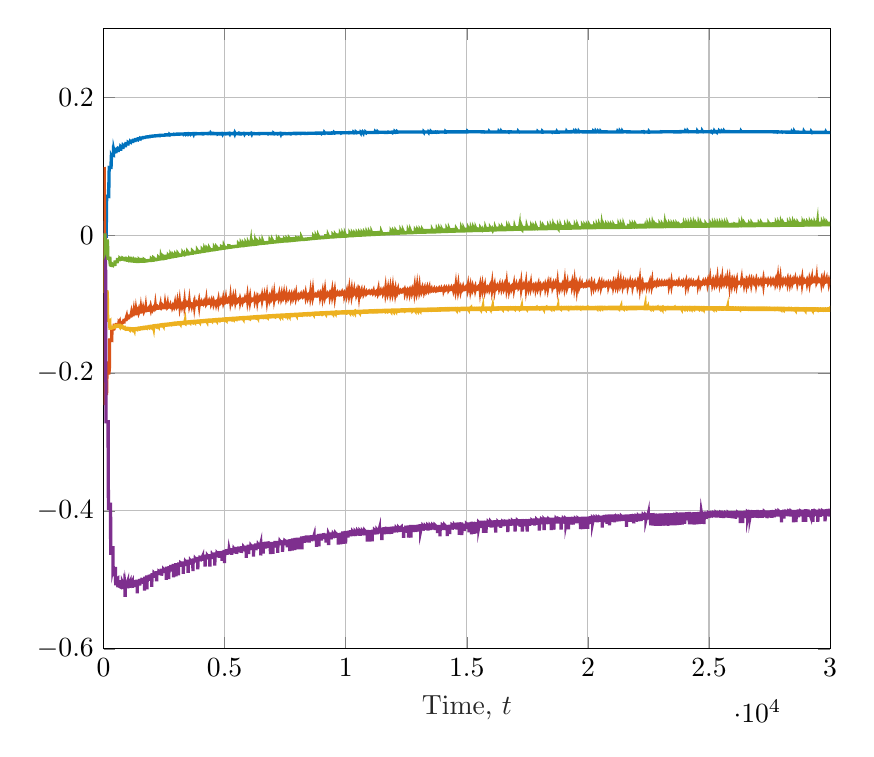
\begin{tikzpicture}

\begin{axis}[%
width=0.761\textwidth,
height=0.65\textwidth,
at={(0\textwidth,0\textwidth)},
scale only axis,
xmin=0,
xmax=30000,
xlabel style={font=\color{white!15!black}},
xlabel={Time, $t$},
ymin=-0.6,
ymax=0.3,
axis background/.style={fill=white},
xmajorgrids,
ymajorgrids
]
\addplot [color=mycolor1, line width=1.2pt, forget plot]
  table[row sep=crcr]{%
0	0\\
2.1429703121903	0.0071388497017324\\
10.2144458867369	0.0071388497017324\\
12.6935285233594	0.0182630793096905\\
19.0024166006078	0.0182630793096905\\
21.6341449197353	0.0155200722547306\\
30.3065932697173	0.0157159249902179\\
33.2579855431177	-0.00130782568521681\\
108.841166682076	-0.00149401539601968\\
111.689288870384	0.0183589851731085\\
117.772474843459	0.0191556906938786\\
120.968578818061	0.0214065269392449\\
125.010576718396	0.049401769436372\\
130.125708129439	0.0512465794490709\\
134.021148090924	0.056102288144757\\
208.472820728439	0.055922178147739\\
211.539249661768	0.0712667731459078\\
219.836383353468	0.0712809293909231\\
224.131150829977	0.092217769659328\\
230.683618784802	0.0928618445432221\\
235.232270739052	0.098088785969594\\
310.101743421972	0.098005542615283\\
313.797145832774	0.106676715018693\\
319.831119357881	0.106676715018693\\
323.171506489693	0.113852398473682\\
329.701819856342	0.113380746995972\\
333.844214006116	0.115329776021099\\
408.020542798851	0.115323296115093\\
411.421409071962	0.120814957335824\\
417.864423662864	0.120395338588423\\
421.373701817352	0.122490657944581\\
431.877165995527	0.120724975087796\\
492.916461167741	0.120681762280583\\
510.868257740993	0.120795243030443\\
515.838572820398	0.124471925173566\\
521.107462027088	0.124564976144029\\
527.87067027939	0.123806445622904\\
531.763767883513	0.122593208227045\\
562.250432220222	0.122526486960851\\
609.683483558674	0.122546779046388\\
614.40414077344	0.125744855700759\\
627.512820855634	0.12555030612566\\
631.853310085095	0.124542370038398\\
678.084923536706	0.124487965353183\\
707.663192768276	0.124502559174289\\
711.877846211777	0.12760395058649\\
719.002974921601	0.127334732034797\\
723.524635392067	0.127750325169472\\
740.872404947742	0.127120364591974\\
806.437082491226	0.127129316460923\\
811.710224354163	0.129786016335856\\
818.729012973348	0.129538829609373\\
822.584666089948	0.130089292004413\\
829.447921885614	0.130126548381668\\
834.249671136608	0.129752841196023\\
908.32016420189	0.129763879263919\\
912.174388348241	0.131679016674752\\
919.376237631674	0.131679016674752\\
924.221934213645	0.132342884026002\\
941.230331266841	0.132143161859858\\
1006.07411180477	0.132159196789871\\
1011.37546106351	0.133840344868076\\
1018.86337179198	0.133618556130386\\
1022.94220741022	0.134339758675196\\
1040.54254986743	0.134163388647721\\
1107.0030412346	0.134169646338705\\
1111.89815581251	0.135528090570006\\
1119.026855753	0.135321325316909\\
1123.41616845127	0.135977576366713\\
1151.18483375865	0.135897598527663\\
1208.17608103233	0.135907849191426\\
1212.79840963939	0.136827820595499\\
1219.90195438917	0.136827820595499\\
1225	0.137403219392581\\
1255.94294843765	0.137357502710074\\
1307.86856223811	0.137364463513222\\
1312.5064435382	0.138053966547886\\
1319.28165371157	0.138053966547886\\
1323.10139945319	0.138459962319757\\
1391.11797563627	0.13847540585266\\
1410.92555771356	0.138232466411864\\
1421.84138523702	0.139584650616598\\
1438.38264153453	0.139540482432494\\
1506.57312321335	0.139547077385942\\
1511.70017968949	0.14012077256848\\
1518.91323295227	0.139967453113059\\
1523.12325550624	0.140533437988779\\
1620.72318385332	0.140942975805956\\
1631.75471775699	0.141547105919017\\
1710.79978572428	0.14154698278071\\
1743.7443238451	0.142194481930346\\
1818.51036044772	0.142293145756412\\
1822.91449497836	0.142599933504243\\
1901.47028032636	0.142776519711333\\
1919.94303399767	0.142804373037507\\
1931.2273978423	0.143364202998782\\
2017.76379775714	0.143319069633435\\
2022.21919173714	0.143547698273323\\
2127.96818706816	0.143763543015666\\
2132.27725086937	0.143998189407284\\
2230.71941612057	0.144203299973015\\
2247.20160580119	0.144363807885384\\
2316.72818066891	0.144175914443622\\
2321.61841416669	0.14471129960657\\
2332.91047548936	0.144769646452914\\
2520.26243371515	0.144842296969728\\
2538.50572915302	0.145314137778769\\
2717.21980816186	0.14531021444418\\
2721.87048550599	0.145863568184723\\
2729.27147467898	0.14564317964323\\
2733.92323082226	0.145897690443235\\
2917.0023110632	0.145821260601224\\
2921.67787110436	0.146328202517907\\
2933	0.146315937152394\\
3229.26479536984	0.146490394741704\\
3240.59900200955	0.146706111769163\\
3309.92693583981	0.14670821818072\\
3314.50315311764	0.146330488649255\\
3327.00391117065	0.146647319848853\\
3338.51577087246	0.146820270176249\\
3409.00607541228	0.146822753707966\\
3412.60160627479	0.146426923001854\\
3423.52180546665	0.146701838257286\\
3469.23213376801	0.146894222947594\\
3506.09107654371	0.146897384267504\\
3510.95060424976	0.146335687037208\\
3516.7830118806	0.146465378711582\\
3521.32582004987	0.147106971213361\\
3532.51270457872	0.14706204689719\\
3608.80539905221	0.147068642396334\\
3612.32217278336	0.146651755330822\\
3622.96847715085	0.14695218169436\\
3684.3313860985	0.147092240615166\\
3710.373441808	0.14709852647502\\
3716	0.146682467027858\\
3721.12245391358	0.147217261870537\\
3732.74690362606	0.14722555492699\\
3808.47611844205	0.147233418618271\\
3812.27498387385	0.146802149432915\\
4029.8779589236	0.147108113382274\\
4053.27416341057	0.147216813555133\\
4109.49806211522	0.147229400437936\\
4113.36759002267	0.146811788799823\\
4120.15878863379	0.146811788799823\\
4131.1192481148	0.147417174463044\\
4271.26430865099	0.147438995125412\\
4309.00323328197	0.147444199865276\\
4312.827772976	0.146988993834384\\
4319.77101667516	0.146988993834384\\
4324.93485008113	0.147498401242046\\
4380.16291541682	0.147709288488841\\
4406.92531620958	0.147710349352565\\
4411.35875606601	0.147328756378556\\
4417.73247370151	0.147293901889498\\
4421.96696244987	0.14770542932456\\
4428.86051845579	0.147378196390491\\
4439.77156477698	0.14756986213979\\
4509.0383319938	0.147581904522667\\
4512.86138130377	0.147141880624986\\
4709.7177956034	0.14714850699238\\
4714.1036375142	0.146737851377111\\
4726.73586135255	0.146983204645949\\
4738.3876561124	0.147134091446787\\
4808.19896336354	0.147140337499877\\
4812.2553915837	0.14670732045488\\
4819.1859545513	0.14670732045488\\
4824	0.14713791658869\\
4883.92308228054	0.147343067197653\\
4910.55972756127	0.1473494181555\\
4916.00330713585	0.146936012042715\\
4921.24138306996	0.147345055698679\\
4931.95844957148	0.147258216595219\\
5007.00093248662	0.147258842040173\\
5011.62899045114	0.146823954724823\\
5018.37065311713	0.146802177347126\\
5022.78953169446	0.14734312571818\\
5108.74627681381	0.147426047038607\\
5113.0343599325	0.146990504861606\\
5119.61561598695	0.146990504861606\\
5124.91453528286	0.147434849783167\\
5209.90839354102	0.147571390061785\\
5216.24543602869	0.1471375166293\\
5221.25546140975	0.147516813154652\\
5232.1260927229	0.147406572501495\\
5308.38793498067	0.147412837974116\\
5312.45721138182	0.146951200382318\\
5319.39422424302	0.146951200382318\\
5323.80358989279	0.147400147965527\\
5382.42780921902	0.147533836170624\\
5409.57733857635	0.147539120163856\\
5415.01853605729	0.14707172267299\\
5421.01659445115	0.147729915450327\\
5427.86478395671	0.147221657811315\\
5442.07664864263	0.147336476748023\\
5507.64115087972	0.147348703125317\\
5512.00259568214	0.146894633944612\\
5616.40172690298	0.146772413067083\\
5621.30468205311	0.147523131290654\\
5632.08739758415	0.14736386775985\\
5707.95140895514	0.147373398944183\\
5712.34631878633	0.146951714767056\\
5730.57022306823	0.147170909396664\\
5744.24033274177	0.147342294963892\\
5810.0902202252	0.147350688886945\\
5816.15466093113	0.146913486834819\\
5821.20237459952	0.147275307437667\\
5831.84173305134	0.147122430455056\\
5929.19897097909	0.147227087949432\\
5939.24298404938	0.147372025174263\\
6007.30525959839	0.147376554530638\\
6012.1447243853	0.146947383327642\\
6030.21780977659	0.147258577493631\\
6043.29076973042	0.147392501887225\\
6109.81703562	0.147399953697459\\
6116.00344287793	0.146967418233544\\
6121.31178211188	0.147482147600385\\
6131.85203342423	0.147264165672823\\
6416	0.146812049897562\\
6421.03520784756	0.147434228401835\\
6431.22904113229	0.147437202955189\\
6751.78603862941	0.147428991582274\\
6809.10110935699	0.147437058236392\\
6813.93890827283	0.1470638836945\\
6831.05502440718	0.14737726410749\\
6868.6467224502	0.147426966814237\\
6906.60931277213	0.14743624386756\\
6911.94791900303	0.147059903094487\\
7017.82212516034	0.146841234545718\\
7021.96836690782	0.14760730218768\\
7032.35024055289	0.147305912334559\\
7108.51371387645	0.147315309837722\\
7112.83159545859	0.146918090598774\\
7119.94133429677	0.146918090598774\\
7131	0.147351934843755\\
7191.0163446273	0.147386914526578\\
7206.82191335597	0.147393657844077\\
7211.84057310519	0.146982307342114\\
7229.63389416331	0.147244696228881\\
7243.22881067909	0.1473439294532\\
7310.89411168927	0.147450353182649\\
7317.74168893769	0.146902997374127\\
7322.02083579929	0.147366015291482\\
7333	0.147226439599763\\
7405.56431418971	0.147232755825826\\
7411.45992800876	0.146880429034354\\
7429.74514620524	0.147156116185215\\
7449.14046552766	0.147247921344388\\
7611.14388079901	0.146918095710134\\
7633.41826141419	0.147201340241736\\
7704.57106112706	0.147208312329894\\
7711.36595432442	0.14681215951714\\
7718.31165196934	0.146800430677104\\
7722.48067772292	0.147210785460629\\
7829.42503329036	0.14746412565728\\
7852.66170164884	0.147527797340445\\
7905.23476009957	0.147535712276294\\
7911.15567496596	0.147166168902913\\
7918.20892673814	0.147145507577079\\
7922.14401669169	0.147658901965769\\
7990.48006294942	0.147733367026376\\
8005.00357152856	0.147741411714378\\
8011.37958121969	0.147348527887516\\
8044.16254031615	0.147583364869206\\
8106.15599899262	0.147591659711907\\
8111.82982684387	0.147190078896529\\
8119.00540560564	0.147170407384692\\
8123.57372794385	0.147745479764126\\
8269.83822618062	0.147641776871751\\
8308.16728886086	0.147647918107396\\
8312.91868559702	0.147234720701817\\
8420.58818214518	0.147206669069419\\
8431.17292306665	0.147678340312268\\
8729.32139585512	0.147806548753579\\
8807.44856303841	0.147839544231829\\
8811.89405545056	0.14752405998297\\
8869.68049735541	0.147822940776678\\
9009.09745142378	0.147826311454992\\
9013.85416619627	0.14744749345482\\
9026.33362305641	0.147760498792195\\
9056.08988484127	0.147821377398941\\
9114.23414617582	0.147506908633659\\
9121.01195749822	0.148467047358281\\
9131.92915517115	0.147992958631221\\
9420.16745903611	0.147769305513066\\
9431.29525080641	0.14822779370661\\
9516.0050167573	0.147885818387294\\
9521.13500243677	0.148625806923519\\
9532.01367893672	0.148319464267843\\
9806.13883715562	0.148296957544517\\
9811.74699103655	0.147964093557675\\
9830.51452389086	0.148229272563185\\
9854	0.148312566107052\\
10120.7545853081	0.148270363024494\\
10131.6222818175	0.148702281992882\\
10316.1556153589	0.148274218066945\\
10321.3919837539	0.149013916994591\\
10332.211355176	0.148697991819063\\
10417.7469963724	0.148360471506749\\
10421.8979925171	0.149131697442499\\
10433	0.148769980398356\\
10610.6625766366	0.148681371938437\\
10617.1220772062	0.148349372833763\\
10621.813189233	0.149027957970247\\
10632.810863959	0.148673275303736\\
10710.6673669835	0.14868353741258\\
10717.6455512177	0.148318767856836\\
10721.8473445434	0.149068073780654\\
10732.9352452412	0.148713011327345\\
10811.0009247094	0.14845289718869\\
10817.8071365345	0.148361758772808\\
10821.9101985973	0.149187752987928\\
10833.3414876574	0.148838431181503\\
11217.6944235344	0.148827783974411\\
11222.0006662482	0.149594482561952\\
11233.1858615523	0.149188501836761\\
11317	0.148878619434981\\
11321.7820358563	0.149607695013401\\
11333.1381017241	0.149228972204583\\
11608.8877882458	0.14919037594882\\
11613.7156802243	0.148882624202088\\
11720.022167838	0.148846892385336\\
11731.1807133905	0.149322322351509\\
11914.0275645939	0.149092180916341\\
11920.895694693	0.148915513753309\\
11927.5819006494	0.149432137804979\\
11951.7891076006	0.149374211610848\\
12015.4737326088	0.149086760698992\\
12021.2317557584	0.149890527842217\\
12032.0121434712	0.149508341455658\\
12117.1485798951	0.14924225921277\\
12121.8236670084	0.14986891080116\\
12132.8852592507	0.149542838196794\\
13210.698692775	0.149437535761535\\
13217	0.149198301787692\\
13221.5901071449	0.149988932422275\\
13232.9061687686	0.149590865450591\\
13410.7296126246	0.149414602074103\\
13417.012313751	0.149134409683029\\
13421.6388809554	0.149673753225215\\
13432.9347136308	0.149325842980033\\
13517.7292969227	0.149062210723059\\
13522	0.149836674321705\\
13533.9389911019	0.149442208414257\\
13711.2552150563	0.1491113058255\\
13718.0029903344	0.14908969755561\\
13722.0503271158	0.149626863912999\\
13818.2368269386	0.149275643019791\\
13822.8124934388	0.14957746998698\\
13859.2722739062	0.149511419371265\\
14117.4025860862	0.149322518114786\\
14122.007407639	0.150065194124181\\
14133.8430911628	0.149700133631995\\
15016.0915212915	0.149675517215655\\
15021.2371223803	0.150245756900404\\
15032.3066374784	0.149826767188642\\
15708.4524200534	0.149693480798305\\
15719.9470970476	0.149480350901285\\
15731.2589920798	0.149612841345515\\
15916.0735731303	0.149484237550496\\
15921.2040183493	0.150001195255754\\
15932.1810432599	0.149507268306479\\
16317	0.149517698850104\\
16321.5897547781	0.15022728970871\\
16332.7687891868	0.149786648704321\\
16416.055977529	0.149583284637629\\
16421.2790418804	0.150265498381486\\
16432.3370418448	0.149736215989833\\
16707.9572428495	0.149572123627877\\
16719.2520929173	0.149386551001953\\
16723.9785046391	0.149764934678387\\
16759.708042575	0.149705861254915\\
17116	0.149393447536568\\
17121.2799671293	0.150103907140874\\
17132.279280251	0.149621500571811\\
17916.3250388274	0.149468014260492\\
17921.4532267201	0.150022133559105\\
17932.8001713184	0.149588302254415\\
18117.3576197058	0.14929422003479\\
18121.8558473103	0.1500514244035\\
18133.5441582504	0.149578665306763\\
18505.6407456067	0.149427431311778\\
18518.1015782541	0.149205315083236\\
18522.5197379783	0.149455569197016\\
18715.8335373007	0.149194949161028\\
18721.1861742546	0.149817326586344\\
18731.9581554258	0.149321701192093\\
19117.1436643781	0.149448484164168\\
19121.7852832871	0.150218021812179\\
19132.925137194	0.149700696514628\\
19320.012880577	0.149671075781953\\
19326.3872052117	0.150056386897631\\
19342.0496159587	0.149945729390311\\
19414.3672070673	0.149758148632827\\
19421	0.150290239293099\\
19431.7558508557	0.149696649477846\\
19516	0.149543301926315\\
19521.1718718575	0.150331338241813\\
19532.0067509614	0.149872617126675\\
19617.6882551574	0.149706693373446\\
19621.9003575912	0.15027776520219\\
19632.9833802659	0.149751779779763\\
20215.9730688005	0.149606067538116\\
20221.1732766805	0.150235999142751\\
20232.1998366623	0.149766877926595\\
20317.0123180531	0.149657964200742\\
20321.6507854216	0.150358280738146\\
20332.0533661824	0.149851881258655\\
20417.3234978122	0.149690349822777\\
20421.7959707443	0.150210588024493\\
20432.8986962638	0.14973887510132\\
20517.0482848641	0.149556904147175\\
20521.6597619186	0.150174141803291\\
20532.8802415508	0.149697688411834\\
21215.3011755993	0.149508196333045\\
21221.1802701434	0.150099540715019\\
21231.9422239065	0.149585706039943\\
21317.2115481803	0.14945858869396\\
21321.6417395426	0.150320275024569\\
21332.3263933206	0.14981181264011\\
21417.351910062	0.149673880758201\\
21421.8266423857	0.150352028187626\\
21432.898581737	0.149807867321215\\
21908.2284091572	0.149530665377824\\
21919.3520714009	0.149394914515142\\
21930.003641338	0.149418455239356\\
22309.7613955523	0.14970066540991\\
22314.9858168694	0.149562443424657\\
22321.0662034484	0.149839804340445\\
22342.8092057293	0.149528568214009\\
22517.1242634101	0.149279045934236\\
22521.7323807462	0.149975053944218\\
22532.7924571718	0.149507797184924\\
23019.1942148502	0.14940173422292\\
23023.9799485888	0.14987298712731\\
23051	0.149780505958915\\
23818.9468793398	0.149684970096132\\
23822.9863168336	0.150145744566544\\
23850.4841732055	0.150078534559725\\
24017.1160364527	0.149973589843285\\
24021.6942214265	0.150516027049889\\
24032.6955024185	0.150007922871737\\
24117.3530203838	0.149813406773319\\
24121.6466749615	0.150487465361948\\
24132.4013769486	0.149943094416813\\
24518	0.149689470319572\\
24522.0020996167	0.150469641364907\\
24533.0037678317	0.149946948098659\\
24718.0313625256	0.149750540953391\\
24722.0016286153	0.150588291042368\\
24733.0989235541	0.149974357926112\\
25109.9520998524	0.149656424637215\\
25115.6937658416	0.149502311192919\\
25121.0913230378	0.15016449252289\\
25143	0.14980605956589\\
25216.0333427894	0.149660259761731\\
25221.2110718401	0.150385856919456\\
25231.9797937119	0.14981295065445\\
25315.4391974248	0.149677203702595\\
25320.9025739178	0.149460640972393\\
25327.2463062733	0.150053373199626\\
25342.4469990413	0.149958592133771\\
25416	0.149792894844722\\
25421.1352214631	0.150572188424121\\
25432.2136457829	0.150126758111583\\
25515.3617295063	0.149987653581775\\
25521.1485498463	0.150498379334749\\
25531.63635359	0.150065205423743\\
25616.2452317043	0.149931996005762\\
25621.2564436163	0.150557157208823\\
25632.1647663355	0.150015386414452\\
26316.8687098101	0.149919577928813\\
26321.4305710401	0.150491032945865\\
26332.3184438609	0.149934226821642\\
27810.2757237357	0.149694014802662\\
27820.8877865944	0.149398262339673\\
27831.8180622961	0.14965244263658\\
28006	0.14954063996629\\
28017.9398934959	0.149379275004321\\
28022.0466987695	0.14957593190411\\
28067.8463567904	0.149406633790932\\
28414.9687831391	0.14921984682951\\
28421.0003162165	0.149855618092261\\
28431.8648451467	0.149394727101026\\
28517.4779562238	0.149262612281746\\
28521.6316079654	0.150008226410137\\
28532.6654438838	0.149396612432611\\
28917.8760863861	0.149105523487378\\
28921.7419887424	0.149923798762757\\
28932.6796630234	0.149318770083482\\
29210.4238771097	0.149010032677324\\
29217	0.148906944246846\\
29221.4878685808	0.149489678045938\\
29232.0066601752	0.148933217100421\\
29816.5308583665	0.148965406704519\\
29821.3596718873	0.149414440587861\\
29832.2137285266	0.14876896286296\\
29998.5116797138	0.148684788811806\\
};
\addplot [color=mycolor2, line width=1.2pt, forget plot]
  table[row sep=crcr]{%
0	0\\
2.1429703121903	0.0959209359534725\\
30.3065932697173	0.0961071037381771\\
33.2579855431177	0.0326556620893825\\
38.856075102387	0.0212785567346145\\
41.1680613500212	0.0047146553042694\\
46.0485718023447	-0.142023967368004\\
52.3843725863771	-0.177788716668147\\
58.0545783998896	-0.246763924606057\\
60.9123342033199	-0.22959320229711\\
117.772474843459	-0.22959320229711\\
120.968578818061	-0.226612948623369\\
130.125708129439	-0.226612928883696\\
134.021148090924	-0.208819801151549\\
140.046488349912	-0.205965136072336\\
144.474555678571	-0.183359787763038\\
150.889071163801	-0.1880390415281\\
156.402175379095	-0.199119066404819\\
161.015668957811	-0.199948387115001\\
219.836383353468	-0.199948387115001\\
224.131150829977	-0.198462997264869\\
230.683618784802	-0.196986009465036\\
235.232270739052	-0.187971109851787\\
240.801411190478	-0.188129158203083\\
246.124790787722	-0.153071140372049\\
251.25142180188	-0.153091240332287\\
257.567764332773	-0.150042559100257\\
261.634361819251	-0.152691012161085\\
319.831119357881	-0.152691012161085\\
323.171506489693	-0.152014212602808\\
329.701819856342	-0.152014212602808\\
333.844214006116	-0.149548296267312\\
340	-0.149778679184237\\
343.99687958898	-0.13815499420889\\
349.994714028755	-0.136834556255053\\
354.107547577307	-0.13423627197335\\
359.712273808556	-0.136005043827026\\
417.864423662864	-0.135995300210197\\
421.373701817352	-0.135491307777556\\
428.077185216498	-0.135491307777556\\
431.877165995527	-0.131650952764176\\
438.729790616377	-0.135560729795543\\
442.278039469038	-0.130693872735719\\
447.766527706597	-0.128451318283624\\
451.090069126785	-0.131080640341679\\
454.746568083894	-0.131253242409002\\
459.793861401424	-0.132386264922388\\
515.838572820398	-0.132386401703116\\
521.107462027088	-0.131928733560926\\
527.87067027939	-0.131928733560926\\
531.763767883513	-0.128160298136208\\
537.742638090127	-0.131627246453718\\
541.344829898393	-0.128906194717274\\
545.355712957917	-0.127380947062193\\
549.864808520368	-0.129801601036888\\
553.661844136259	-0.130914600518736\\
558.915672403396	-0.131650143179286\\
568.769765201821	-0.131489558076282\\
620.745964045225	-0.131190939318913\\
627.512820855634	-0.131116267351899\\
631.853310085095	-0.127899700812122\\
638.43375335271	-0.130660153205099\\
642.190589693146	-0.126715544880426\\
647.81676004254	-0.126934283729497\\
651.723239909541	-0.126667990807618\\
657.50593916958	-0.129582945883158\\
681.353659528068	-0.129521711231064\\
730.368192559952	-0.129251550468325\\
740.872404947742	-0.127129813499778\\
745.219982828661	-0.124498015622521\\
750.577034095531	-0.126092011345463\\
755.857574539285	-0.126494141168223\\
777.00290432771	-0.126403293463227\\
829.447921885614	-0.126217210203322\\
834.249671136608	-0.124952142370603\\
840.373504782932	-0.12505883167978\\
844.419693614942	-0.121747133547615\\
850.11647017195	-0.123163390857371\\
890.755841466762	-0.122978063831397\\
930.649139281082	-0.122742062998441\\
941.230331266841	-0.120473188260803\\
947.693673079786	-0.119132433334016\\
951.83587583917	-0.118652469496737\\
958.046247733331	-0.120043556038581\\
972.315610546346	-0.11994854371369\\
1029.90835891964	-0.119864008025615\\
1034.98903117405	-0.118672196160333\\
1040.54254986743	-0.118714141455712\\
1046	-0.116236016780022\\
1050.98992346409	-0.117751999958273\\
1061.24069831668	-0.117301584868983\\
1130.31443625383	-0.117255793036747\\
1135.65246562484	-0.116060714521154\\
1140.93931589019	-0.115450199406041\\
1146.62482579601	-0.114416214128141\\
1151.18483375865	-0.115364897636027\\
1179.01126471064	-0.115390663133439\\
1225	-0.11538004076283\\
1230.76274806616	-0.114449627173599\\
1240.66882618296	-0.114133258852235\\
1245.87698656711	-0.11285612390202\\
1250.55622544931	-0.114277568092803\\
1261.04291372417	-0.114024587546737\\
1329.86104208577	-0.114021805817174\\
1333.86155719839	-0.112949520931579\\
1339.59939138869	-0.112724676011567\\
1343.48228525082	-0.111344815279153\\
1349.54322408807	-0.112777936625207\\
1359.60071979818	-0.112945073913579\\
1363.7272661763	-0.112613914574467\\
1428.82206480029	-0.112618734186981\\
1432.19104398142	-0.111530997266527\\
1438.38264153453	-0.111290907887451\\
1441.97099862661	-0.110486263649364\\
1448.20541566692	-0.110856644958403\\
1452.06755204638	-0.110360964197753\\
1458.6929682482	-0.111697961594473\\
1462.07847445008	-0.111394178340561\\
1530	-0.111419453936833\\
1534.0987541984	-0.110181297004601\\
1539.65032105379	-0.110040164228849\\
1543.6070206236	-0.108813618604472\\
1549.51633679582	-0.110450101372408\\
1553.30815745178	-0.110735961454338\\
1572.49889027333	-0.110480458100938\\
1627.1243450965	-0.110511082049925\\
1631.75471775699	-0.109574015037651\\
1638.08584955521	-0.10923239944168\\
1642.00687855725	-0.108336064757168\\
1648.26922146963	-0.109315065354167\\
1652.21906805947	-0.109326946589135\\
1658.6621467859	-0.110078071753378\\
1662.66893467667	-0.109670955083857\\
1728.79962268898	-0.109708710104314\\
1733.12922262778	-0.108582550190476\\
1739.56512403056	-0.108154370209377\\
1743.7443238451	-0.107018091443024\\
1749.7311371381	-0.108999595606292\\
1759.91465074835	-0.108831011595612\\
1829.92032747495	-0.108870325024327\\
1834.82217032371	-0.107562023884384\\
1846.22153867136	-0.107002619122795\\
1851	-0.108129520460352\\
1860.74322548409	-0.107940320267517\\
1926.03348978527	-0.107968617725419\\
1931.2273978423	-0.10702704248979\\
1937.78120462559	-0.106592208961956\\
1941.96149228081	-0.105852157183108\\
1948.12226568695	-0.106753017553274\\
1951.97553377745	-0.106069526129431\\
1958.11043262636	-0.107054389478435\\
1972.52087569288	-0.106970838754933\\
2029.32100501169	-0.107002334767458\\
2033.90819169728	-0.105958519216074\\
2046.0034418327	-0.105439346192725\\
2050.76334812981	-0.106863134547893\\
2056.00342556328	-0.106552049062884\\
2071.47548154816	-0.106667380354338\\
2127.96818706816	-0.106710476513399\\
2132.27725086937	-0.105831049666449\\
2139.01312156839	-0.105324597367144\\
2142.7315033376	-0.104149734015664\\
2149.04603674252	-0.105961256533192\\
2152.78893863173	-0.105795500348904\\
2158.86604718418	-0.106407349841902\\
2169.71362382936	-0.106198612091248\\
2230.71941612057	-0.106126952890918\\
2236.90995947508	-0.10490721442693\\
2241.38029792706	-0.104412092052371\\
2271.43428933035	-0.105581823354441\\
2328.83566180742	-0.105635477026226\\
2332.91047548936	-0.104686565806333\\
2339.50504133006	-0.104191418253322\\
2343.80653338398	-0.103460589853057\\
2349.46446689618	-0.105400446354906\\
2359.25692482376	-0.105713983532041\\
2363.35022257851	-0.10537373578336\\
2424.17948257758	-0.105410941210721\\
2431	-0.104575454657606\\
2437.34417895164	-0.104179545563966\\
2441.67777844047	-0.103542300734262\\
2467.06276130875	-0.10510975671059\\
2527.21198669675	-0.105164245549531\\
2531.95625267276	-0.104178351335577\\
2538.50572915302	-0.103619510813587\\
2542.33328867969	-0.102426751629537\\
2548.24850962279	-0.103860816398083\\
2552.16902505396	-0.103954847949353\\
2558.10381614968	-0.104557598071551\\
2572.24985082022	-0.104468482386437\\
2628.59969442289	-0.104513405887701\\
2633.0178668212	-0.103539035128051\\
2639.74385113236	-0.103042354639911\\
2643.3356539065	-0.102388243791211\\
2649.00728168863	-0.104088461765059\\
2652.42114148101	-0.10393974039107\\
2662.33827069417	-0.104314986878308\\
2729.27147467898	-0.104374225484207\\
2733.92323082226	-0.103396227663325\\
2743.92005217004	-0.102575105880533\\
2749.31943362875	-0.103849326267664\\
2759.01311924212	-0.104122256107075\\
2763.25693350876	-0.103844871118781\\
2829.79182787078	-0.10388256002625\\
2835.16444759464	-0.102552506268694\\
2844.016173026	-0.102392442426208\\
2849.40549482055	-0.103601176168013\\
2853.00634138237	-0.103291722640279\\
2858.73984368716	-0.103829491690703\\
2862.88422507771	-0.103583959386015\\
2928.60375440571	-0.103637438132864\\
2933	-0.102692602795287\\
2939.81552733111	-0.102165364176471\\
2943.6996673279	-0.101498599091428\\
2949.14859679667	-0.103106351845781\\
2952.35600684679	-0.10289176954393\\
2962.2831337896	-0.103109764208057\\
3029.07312743537	-0.103160459784704\\
3033.62986527287	-0.102090184383997\\
3039.79884956768	-0.101696948855533\\
3043.66597899804	-0.100811209686071\\
3049.23767253396	-0.102538980219833\\
3052.8264182937	-0.102333447313868\\
3062.36461098883	-0.102491765832383\\
3128.09856334825	-0.10254180080301\\
3132.08592397109	-0.101565107586794\\
3138.83180587057	-0.101121677838819\\
3142.26929304341	-0.100112743089994\\
3148.00422267788	-0.102002296309365\\
3151.4096149136	-0.101306634660432\\
3161.09762071128	-0.102146977071243\\
3229.26479536984	-0.102209420118015\\
3234	-0.101066929299122\\
3240.59900200955	-0.100750068388152\\
3244.53344166362	-0.101006296805281\\
3249.7250084254	-0.10213042754549\\
3253.13145457137	-0.101733531770151\\
3258.7959171048	-0.102187614495051\\
3262.82084595679	-0.101889915833453\\
3327.00391117065	-0.101953111152397\\
3331.79647791024	-0.100941002881882\\
3338.51577087246	-0.100511437201931\\
3342.26093165005	-0.0994286553213897\\
3347.82420693314	-0.101489695338387\\
3351.38613238964	-0.100856345539796\\
3361.00101084223	-0.101542469732522\\
3430.06874570972	-0.101608365683205\\
3436.00344218671	-0.100280118713272\\
3441.00695998884	-0.0998209878343914\\
3446	-0.10025814747496\\
3450.01434888058	-0.101577736095351\\
3469.23213376801	-0.101223208199372\\
3528.32770629848	-0.101286709341366\\
3532.51270457872	-0.10046846250043\\
3539.22165062591	-0.0999426892776683\\
3542.74872436703	-0.0988412531078211\\
3548.32105712704	-0.10066502992413\\
3551.97099319949	-0.10018433877849\\
3561.27952742534	-0.10107390873236\\
3629.82837361279	-0.101147948258586\\
3635	-0.0998320700600743\\
3644.5088083644	-0.0998439150243939\\
3649.66265671154	-0.100837446916557\\
3652.89449475812	-0.100364463527512\\
3668.00331368189	-0.100657186660101\\
3728.16968269358	-0.100722075087106\\
3732.74690362606	-0.0998612474395486\\
3743.02257541929	-0.098590257075557\\
3748.7544227753	-0.100457127256959\\
3752.03286567183	-0.0995419322680391\\
3761.27670604578	-0.100316736934474\\
3829.96083016896	-0.100383454329858\\
3836	-0.0991253389256599\\
3841.12971036832	-0.0987595423393941\\
3846.26648357925	-0.099217961087561\\
3850.33223347291	-0.100441032758681\\
3863.25520111353	-0.100171416688681\\
3928.28130103319	-0.100236297064839\\
3932.68411641294	-0.0993536622372631\\
3939.29043884383	-0.0989773594956205\\
3942.88294529316	-0.0983525465780986\\
3948.86415551575	-0.100037149160926\\
3952.12346220194	-0.0991081172796839\\
3957.15676172539	-0.0998028745707416\\
3966.62653886499	-0.100001935014006\\
4029.8779589236	-0.100078088809823\\
4035.80573389588	-0.0987985511710576\\
4040.76785759918	-0.0983524775037949\\
4044.64782244763	-0.0988839892816031\\
4049.82343968829	-0.100019317815168\\
4078.95464740375	-0.0995878455942147\\
4126.07403544831	-0.0996598763013026\\
4131.1192481148	-0.0987965836793592\\
4141.78612336691	-0.0978686319722328\\
4147.56361329904	-0.0987206264871929\\
4151.33871470614	-0.0985360444792605\\
4154.83607408533	-0.0991283416515216\\
4163.90520474617	-0.0993371507574921\\
4229.01689651387	-0.0994123275486345\\
4233.35662614447	-0.0983558065745456\\
4239.96295366641	-0.0979921681282576\\
4243.35417778067	-0.0970925830370106\\
4249.21803284427	-0.0989520414805156\\
4252.69929817252	-0.0987377020683198\\
4271.26430865099	-0.0988303620288207\\
4324.93485008113	-0.0988878637508606\\
4330.85649400827	-0.0979375996103045\\
4341.21037788334	-0.0970949151851528\\
4350.50664633387	-0.0989515991641383\\
4391.24785145948	-0.0986200611660024\\
4428.86051845579	-0.0986767523099843\\
4432.97876076237	-0.0976763177095563\\
4443.07087693282	-0.096718777447677\\
4449.0298897647	-0.0983046165929409\\
4452.34729749643	-0.0980006342906563\\
4467.14174784977	-0.0982714614183351\\
4530.72785846018	-0.0979464009506046\\
4541.28185642152	-0.0966415647199028\\
4546.63393687929	-0.0973503699424327\\
4551.12499528719	-0.0985067266447004\\
4554.1199873136	-0.0981732508880668\\
4559.22550630149	-0.0983363721752539\\
4563.21280838384	-0.0980755364325887\\
4629.90562375734	-0.0981401729877689\\
4635.21514278452	-0.0968263070571993\\
4640.634208407	-0.0966448892650078\\
4644.47180684014	-0.0969150712917326\\
4649.72343677032	-0.0979776310814486\\
4652.86506552183	-0.0974702030543995\\
4667.68332508349	-0.0975551475457905\\
4726.73586135255	-0.0976320017653052\\
4731.51260374806	-0.0966901049287117\\
4738.3876561124	-0.0963464378546632\\
4742.09721022311	-0.0956891608584556\\
4747.8522150176	-0.0972098130660015\\
4751.41846702668	-0.0966006895141618\\
4760.1838975986	-0.0973921793047339\\
4830.48381420751	-0.0974581514237798\\
4836.03350604084	-0.0961170145747019\\
4840.91748290742	-0.0956813822776894\\
4845.26536010232	-0.0962390146887628\\
4850.64649822661	-0.0973559770573047\\
4862.71745356912	-0.0968614067860472\\
4927.92909596712	-0.0969287813568371\\
4931.95844957148	-0.0959968508577731\\
4938.81801268894	-0.095820895738143\\
4942.04054126195	-0.095120493122522\\
4948.18710877003	-0.0964778996676614\\
4951.77425677891	-0.0960498601016297\\
4960.28989055551	-0.0967304210171278\\
5029.61561215179	-0.0968034072066075\\
5033.88725178999	-0.0957660076419415\\
5040.02683326294	-0.0953987408756802\\
5043.35398406207	-0.0947294241632335\\
5049.15801722012	-0.0966034496814245\\
5057.55489448957	-0.096301754743763\\
5070.90711728311	-0.0963943042879691\\
5130.56336047161	-0.0964746431563981\\
5136.31707765498	-0.0951915363548324\\
5141.0756308044	-0.0948201917854021\\
5145.11442350142	-0.0953983203980897\\
5150.53384580279	-0.0966106119194592\\
5172.1854186452	-0.0961748211993836\\
5228.00988112635	-0.0962337564124027\\
5232.1260927229	-0.0952574591974553\\
5238.80800988311	-0.0948805084735795\\
5242.23545242564	-0.0937645369340316\\
5248.15888714893	-0.0958505924645578\\
5251.68885389107	-0.0952783366556105\\
5259.98668477049	-0.0959960651380243\\
5329.94670894251	-0.096062431424798\\
5334.45168538485	-0.094820551428711\\
5340.42889531568	-0.0945975505637762\\
5343.78146229533	-0.0939822031432413\\
5349.21322739687	-0.0957916920815478\\
5352.4149777751	-0.0955472607201955\\
5378.25614234969	-0.0956272765142785\\
5427.86478395671	-0.0957077629936975\\
5432	-0.0947340936036198\\
5438.63669331452	-0.0943778058390308\\
5442.07664864263	-0.0936481098688091\\
5447.84897313344	-0.0952970578582608\\
5451.58595579535	-0.0947436243004631\\
5455.69732534187	-0.0953172277077101\\
5469.78283363634	-0.0954322829420562\\
5530.32593737709	-0.0955033461214043\\
5535.353587993	-0.0942348973949265\\
5540.67438988352	-0.0940502832818311\\
5544.43703722425	-0.0944823589888983\\
5549.79476783698	-0.0958440817485098\\
5562.31161613313	-0.0953857180647901\\
5628.14688225833	-0.095453614667349\\
5632.08739758415	-0.0944649477969506\\
5638.50686246919	-0.0940883160510566\\
5641.85999704869	-0.0935021707155101\\
5647.44793161612	-0.0941690215731796\\
5651.0898875838	-0.0954776210601267\\
5654.38573660336	-0.0950187711496255\\
5712.34631878633	-0.0950695060237194\\
5730.57022306823	-0.0951360056678823\\
5735.14588095582	-0.0938054140679014\\
5740.63636198901	-0.0935959949638345\\
5744.24033274177	-0.0938671848016384\\
5749.62103490747	-0.0949399418605026\\
5753.00133070859	-0.0945593964024738\\
5778.92916837699	-0.0946853664318041\\
5827.90510599863	-0.0947566597897094\\
5831.84173305134	-0.0936030432858388\\
5838.20539609893	-0.0934333213408536\\
5841.60052096805	-0.09297683560726\\
5846.69434980799	-0.0935998708919215\\
5850.53475668044	-0.0948267161838885\\
5868.75612240158	-0.0943622275699454\\
5929.19897097909	-0.0944364105125715\\
5932.91551417181	-0.0935451882542111\\
5939.24298404938	-0.093164622077893\\
5942.21124151164	-0.0923075936880196\\
5948.0874389544	-0.0941803990717744\\
5951.57326014749	-0.0934946903653326\\
5955	-0.0940958304672677\\
5969.71517806145	-0.094217838061013\\
6030.21780977659	-0.0942758594028419\\
6034.25596413067	-0.09305385713742\\
6039.99326896522	-0.0928615577613527\\
6043.29076973042	-0.0922392860193213\\
6049.06050294709	-0.0940251122701738\\
6052.17082061917	-0.0934017858198786\\
6061.27570202228	-0.0938375798541529\\
6128.00407011178	-0.093901297004777\\
6131.85203342423	-0.0928406793827889\\
6146.24355857948	-0.0927741407467693\\
6149.99908266528	-0.0939756965162815\\
6163	-0.093588228290173\\
6228.82732623683	-0.0936619964304555\\
6232.52331294271	-0.0928105969032913\\
6238.68212404762	-0.0924093638495833\\
6242	-0.0918059452997113\\
6247.50312595516	-0.0925720573141007\\
6251.12513230283	-0.0936549300895422\\
6254.4806715774	-0.0931808073910361\\
6287.70370254279	-0.093242020739126\\
6329.83557088863	-0.0933252891700249\\
6333.93838897652	-0.0922626142601075\\
6343.12252936117	-0.0916239498983487\\
6348.87826149031	-0.0933061947725946\\
6352.14810697208	-0.0925377905914502\\
6357.75013962637	-0.0931742383327219\\
6389.41509017137	-0.0932215167522372\\
6427.24622546151	-0.0932961546895967\\
6431.22904113229	-0.0923619737550325\\
6441.08514192636	-0.0916240611695684\\
6444.96829338128	-0.0922718683432322\\
6449.73989890783	-0.0935139324974443\\
6463.14619087066	-0.093036055113771\\
6529.24108093148	-0.0931099841945979\\
6532.82864414021	-0.0921419421974861\\
6538.83507605977	-0.0918049006977526\\
6542.02079675463	-0.0911766356730368\\
6547.78229529028	-0.0926400302923867\\
6551.23755401937	-0.0920117221139662\\
6554.96090225094	-0.092499334106833\\
6569.75783901658	-0.0926464640324411\\
6629.26687112937	-0.0927231637760997\\
6632.81817354002	-0.0917459234733542\\
6638.89086414533	-0.0913614149867499\\
6642.14419715729	-0.0907240954511508\\
6647.85884873579	-0.092241705795459\\
6665.01017432494	-0.0923693583863496\\
6729.83854316744	-0.0924412050226238\\
6733.20696353324	-0.0913716276154446\\
6739.5660130627	-0.0910224209364969\\
6742.89227811353	-0.0902390028495574\\
6748.65741761952	-0.0921754283153859\\
6751.78603862941	-0.0913680859302985\\
6761.23468995087	-0.0921610789700935\\
6826.18579227819	-0.0922372437198646\\
6831.05502440718	-0.0913231741578784\\
6840.76408561203	-0.0904510252657929\\
6849.52537519608	-0.0921951867785538\\
6852.8778315084	-0.091723788431409\\
6858.689660998	-0.0921088660616078\\
6862.35982076012	-0.0918798391612654\\
6930.47245201499	-0.0919634473430051\\
6934.62872837799	-0.0907431487867143\\
6940.25440912814	-0.0905473713755782\\
6943.77890573128	-0.0898671683098655\\
6949.2178043124	-0.0917206784361042\\
6952.74962373467	-0.0914897767252114\\
6962.33605650425	-0.0915389688670984\\
7028.90209196011	-0.0916292283109215\\
7032.35024055289	-0.0906657091763918\\
7038.95132244189	-0.0902766968756623\\
7042.67444714928	-0.0892469503778557\\
7048.16385447968	-0.0911605115616112\\
7051.34845194612	-0.0905686462210724\\
7056.15425984807	-0.0910766078486631\\
7101.78097701937	-0.0911111528694164\\
7126.03352888469	-0.0911837461680989\\
7131	-0.0902182476238522\\
7141.13841674111	-0.0894972998758021\\
7146.00343821432	-0.0901981410388544\\
7150.00596277533	-0.0913835530627694\\
7163.12294750191	-0.0909101086690498\\
7229.63389416331	-0.0909671071312914\\
7233.35114699469	-0.0898690390567936\\
7239.57291541732	-0.0894889359806257\\
7243.22881067909	-0.0888755709311226\\
7249.00437470166	-0.0908265144425968\\
7252.32340699316	-0.0905278606624051\\
7267.88308608561	-0.0907328172215784\\
7329.21560470596	-0.0908085817136453\\
7333	-0.0898413788818289\\
7339.70205296296	-0.0894613601958554\\
7343.21101931994	-0.0888659007687238\\
7348.98212703089	-0.0907722187439504\\
7352.27965570206	-0.0904324762595934\\
7372.07853170885	-0.09067688835421\\
7429.74514620524	-0.0907475875537784\\
7433.94255166211	-0.0895549372326059\\
7440.17647700487	-0.0892903252315591\\
7443.68209932042	-0.0885893135637161\\
7449.14046552766	-0.0903989281723625\\
7452.34594120357	-0.0902069160620158\\
7472.00972585416	-0.09032372152069\\
7529.24906333203	-0.0903971466141229\\
7533.11448112628	-0.089240668079583\\
7539.71916842205	-0.0888999070048158\\
7543.41558079331	-0.088266909984668\\
7549.07725051966	-0.090006946840731\\
7552.24553552417	-0.0896316440594092\\
7568.06713317281	-0.0898332010001468\\
7629.28871792482	-0.0899133276834618\\
7633.41826141419	-0.0888850574847311\\
7643.71819500744	-0.0879506758756179\\
7649.14107610699	-0.0898165965409135\\
7652.4007648167	-0.0895865973834589\\
7683.75500402982	-0.0897707079711836\\
7729.39999448708	-0.0898500830699049\\
7733.74841812669	-0.0888831482043315\\
7743.82407173501	-0.0879442617333552\\
7749.22828568221	-0.0897034276458726\\
7752.71839809072	-0.0892484089490608\\
7758.69270137218	-0.0897155854327139\\
7762.25294382764	-0.0895134298989433\\
7829.42503329036	-0.0895747808935994\\
7833.93388454777	-0.0884596174182661\\
7843.77392009217	-0.087521408295288\\
7849.17143329839	-0.0896182319920626\\
7852.66170164884	-0.0892988256382523\\
7862.33109697905	-0.0893779265061312\\
7929.12593395344	-0.0894541149209545\\
7933.13098932614	-0.0882642976976058\\
7939.82321501239	-0.0879510669619776\\
7943.2475193337	-0.0873526831528579\\
7948.88794124738	-0.0891739479557145\\
7952.19727361415	-0.0887404049681209\\
7968	-0.0890366081621323\\
8029.39593706119	-0.0891084549948573\\
8033.8336712896	-0.0881240389971936\\
8040.44787802298	-0.0877704248341615\\
8049.26271145316	-0.0890714042798209\\
8052.86005316363	-0.0887377284925606\\
8058.81573343272	-0.0890955267495883\\
8062.89915264337	-0.0887702367763268\\
8129.95415347314	-0.0888549580668041\\
8135.21083553034	-0.0875139037270856\\
8140.92427687591	-0.0870850460851216\\
8145.01032263407	-0.0877982399833854\\
8149.81338290698	-0.0890014801334473\\
8163.51860146417	-0.0885462488404301\\
8230.52899084135	-0.0886123109230539\\
8236.3588659054	-0.0874088698983542\\
8241.15180775935	-0.086932160458673\\
8246.22408771836	-0.0877937783843663\\
8250.28508311085	-0.088976450930204\\
8264.47257959504	-0.0885191105262493\\
8325.31840384163	-0.0885930008844298\\
8331.04443288585	-0.0876292322209338\\
8337.89307131708	-0.0872994559722429\\
8341.89004828444	-0.0865584753191797\\
8351.12167351744	-0.0887036916574289\\
8355.08354987765	-0.0881200027979503\\
8366.00343662616	-0.0883694682270288\\
8426.61293348562	-0.088452492345823\\
8431.17292306665	-0.0875542528046935\\
8441.81778693545	-0.0870068745753088\\
8447.27550989978	-0.0874187247572991\\
8451.16575655456	-0.088611095543456\\
8456	-0.088096001669328\\
8465.8138428541	-0.0883109477726975\\
8526.78422376345	-0.0883854193198204\\
8531.57285420648	-0.0873186458193231\\
8538.50308889113	-0.0870076988285291\\
8542.55671071594	-0.0859203559921298\\
8548.10754794162	-0.0879877352635958\\
8551.67855751158	-0.087362035013939\\
8561.02369465495	-0.0881438877331675\\
8627.77183382549	-0.0882234699492983\\
8631.82749902236	-0.0872060581787082\\
8638.66183781	-0.0869313722323568\\
8642.70697451181	-0.0856770309437707\\
8648.27390441773	-0.0877932069488452\\
8651.96409830147	-0.0872220155579271\\
8657.79188830714	-0.0879702390666353\\
8671.77581770131	-0.0880539196041354\\
8729.32139585512	-0.0881470797066868\\
8734.43381328576	-0.0869059636279417\\
8740.62809812792	-0.0866541693576437\\
8744.51322483216	-0.0870437436387874\\
8749.51996900238	-0.088017360521917\\
8798.00160573491	-0.0875762942159781\\
8829.96896186897	-0.0876457937702071\\
8835.05966305844	-0.0862851164274616\\
8840.88459087619	-0.0858486183569767\\
8845.81312573562	-0.0866408703295747\\
8850.00680556456	-0.0877380253332376\\
8873.91246618244	-0.0873097135954595\\
8924.55475479965	-0.0873873592863674\\
8941.70857279851	-0.0857014286302729\\
8947.01892066791	-0.0863925486373773\\
8950.759972908	-0.0876251223271538\\
8954.4361084928	-0.0870850905048428\\
8970.00318278553	-0.0872404712936259\\
9026.33362305641	-0.0873299655540904\\
9031.19905893485	-0.0863738395019027\\
9037.84929866896	-0.0860820394846087\\
9041.95911320615	-0.0852933081405354\\
9047.82524692242	-0.0871039179583022\\
9051.321028646	-0.0863062707649078\\
9060.82442062577	-0.0871220791523228\\
9127.79891103159	-0.0872074941944447\\
9131.92915517115	-0.0862366925975948\\
9138.7269846102	-0.0859053135791328\\
9142.78656949725	-0.0847431938309455\\
9148.35867662798	-0.086658016549336\\
9151.8619710475	-0.0861480231360474\\
9157.71968619319	-0.0868657764985983\\
9183.86093754267	-0.0868146547145443\\
9229.28887592078	-0.086902113569522\\
9233.42505716318	-0.085800179916987\\
9240.35518186052	-0.0853882413211977\\
9244.71841446197	-0.0858171096442675\\
9249.73217708032	-0.0870375680024154\\
9263.37631492884	-0.086465183954715\\
9330.63170282285	-0.0865235854616913\\
9337	-0.0852751706916024\\
9341.7271890387	-0.084875691896741\\
9346.851000566	-0.0854904526968312\\
9350.59616331341	-0.0868370648204291\\
9354.22245468974	-0.0862792956831981\\
9370.00322640764	-0.0864054653466155\\
9426.09151957415	-0.0864984672480205\\
9431.29525080641	-0.0854830400858191\\
9438.18024030204	-0.0851810038329859\\
9442.18884229226	-0.0841961113583238\\
9447.90071888378	-0.0860526232499979\\
9451.38401186038	-0.0854478781075159\\
9461.10881222173	-0.0861521355473087\\
9528.01380709382	-0.0862341672436742\\
9532.01367893672	-0.0853194663941395\\
9539.00886099961	-0.0849666825306485\\
9542.83347956526	-0.0841590972195263\\
9548.71469351898	-0.0862025427813933\\
9552.08707747722	-0.0853084281698102\\
9557.92744281182	-0.0860006441107544\\
9578.82519576044	-0.0859240477184358\\
9629.38393914323	-0.0860030491858197\\
9633.82254658205	-0.0849992670518986\\
9640.47164632896	-0.0846060448639037\\
9649.44413478818	-0.0862026105751283\\
9662.8427836658	-0.0859380946640158\\
9729.62323830972	-0.0860141842422308\\
9734.00211585267	-0.0848975748413068\\
9740.61491776013	-0.0845519875620084\\
9753.40343436475	-0.0859595394940698\\
9763.21816461303	-0.0857134008292633\\
9830.51452389086	-0.085806502662308\\
9836.1559983045	-0.084416168712778\\
9841.10893234802	-0.0840130223805318\\
9846.14464471166	-0.0847247164674627\\
9850.30227450835	-0.0858408678504929\\
9869.76972222171	-0.0854797833962948\\
9930.33251123708	-0.0855693795783736\\
9935.9630727448	-0.0843514827356557\\
9941.13153148618	-0.0839539170592616\\
9946.67078748275	-0.084372027842619\\
9950.53219835033	-0.0858382284204708\\
9954.1803233434	-0.0853681543849234\\
10008.2182446567	-0.0854075857059797\\
10026.3886868416	-0.085489078934188\\
10031.219717424	-0.0845060670180828\\
10038	-0.0841714099551609\\
10041.8553415446	-0.0836254133864713\\
10047.6439254221	-0.0851544808574545\\
10051.3438942941	-0.0846144375573203\\
10061.0708358488	-0.0852932008529024\\
10127.4426849251	-0.0853803708778287\\
10131.6222818175	-0.0844062477081025\\
10138.4450977112	-0.0840279998337792\\
10142.3369468469	-0.0829188620955392\\
10148	-0.0850289982918184\\
10151.5564491337	-0.0844498826154449\\
10161.2176201849	-0.0851466062558757\\
10228.1008239545	-0.0852316596501623\\
10232.1642767605	-0.0843496313973446\\
10239.2328354725	-0.083916440824396\\
10242.903453546	-0.083071556276991\\
10248.6473427129	-0.0850731032005569\\
10252.153788382	-0.084397762802837\\
10258.0044675713	-0.0850397009417065\\
10293.1962059708	-0.0850004942731175\\
10328.2095338845	-0.0850755564824794\\
10332.211355176	-0.0841611740543158\\
10339.1308168117	-0.0837679897413182\\
10342.8680148707	-0.0830871355829004\\
10348.5507037564	-0.0848236353667744\\
10352.1955299796	-0.0846719914152345\\
10361.9919847476	-0.0849932615201396\\
10428.9660603982	-0.0850746167961915\\
10433	-0.0840549636923242\\
10443.4416136611	-0.0829310498957057\\
10449.0059264191	-0.0849053097372234\\
10452.3078741814	-0.0845740079676034\\
10471.9744488853	-0.0847525712197239\\
10528.8642141357	-0.0848499349667691\\
10532.8151368337	-0.0838716866710456\\
10543.0722553705	-0.0829305137776828\\
10548.6766508834	-0.0848108233549283\\
10552.0509612404	-0.0837701892123732\\
10557.910370329	-0.0845171381370164\\
10599.9665657153	-0.0844830815076421\\
10629.004047425	-0.084572314604884\\
10632.810863959	-0.0836462146471604\\
10643.0055233063	-0.0825734636564448\\
10648.7373729286	-0.0844744420937786\\
10652.2726025825	-0.0842357893270673\\
10668.1632228276	-0.0842949075558863\\
10728.9983007911	-0.0843716997733281\\
10732.9352452412	-0.0833807795752364\\
10743.7021126294	-0.0824235213694919\\
10748.8081591137	-0.0842543659891817\\
10752.2827228346	-0.0839951236412162\\
10768.1854420224	-0.0841154649569944\\
10829.2706786626	-0.0842019137016905\\
10833.3414876574	-0.0832145209315058\\
10840.0421657973	-0.0828078984995955\\
10849.3035821869	-0.0841327891248511\\
10853.0359756233	-0.0839132931723725\\
10859.0156397814	-0.0841869851428783\\
10863.1867382813	-0.0839227046562883\\
10929.9105088777	-0.0840098692096944\\
10934.610822389	-0.0827409277371771\\
10940.5665160715	-0.0824956471005862\\
10949.2955472347	-0.0839267599403684\\
10969.0461465679	-0.0837874708849995\\
11029.9241847948	-0.083873908224632\\
11034.5413057981	-0.0825787517460412\\
11040.648719582	-0.0823167836242646\\
11044.8877408515	-0.082785498809244\\
11049.8581900692	-0.0839510538171453\\
11069.7251051483	-0.0834987284906674\\
11129.9971223092	-0.0835916406504111\\
11135	-0.0822069661699061\\
11140.7195021966	-0.0817097375693265\\
11144.8486280081	-0.0825807399160112\\
11149.771430539	-0.0839895073841035\\
11163.2436652765	-0.0834981008520117\\
11229.2834169552	-0.0835793557525903\\
11233.1858615523	-0.0824527499062242\\
11243.9649428197	-0.082126121960755\\
11249.2062638995	-0.0835251043135941\\
11252.9256586434	-0.0833022115111817\\
11258.8122139607	-0.0835763371542271\\
11262.3593862605	-0.0833310466114199\\
11329	-0.0834217308547522\\
11333.1381017241	-0.0823163994282368\\
11339.9684319234	-0.0819592426305462\\
11343.739525363	-0.081309137698554\\
11349.1521772452	-0.0833407619029458\\
11352.6673051237	-0.0830536884277535\\
11362.2090303686	-0.0831226744085143\\
11429.8241670179	-0.0832182137382915\\
11434.6551133428	-0.0818967343802797\\
11440.7206055667	-0.0814152166203712\\
11445.4966444249	-0.0820703158678953\\
11449.9846207463	-0.083424292071868\\
11464.1036426941	-0.0828723418126174\\
11524.9141259423	-0.0829611566805397\\
11537.1934166504	-0.0815309709323628\\
11541.741299965	-0.0811069562623743\\
11547.2105985643	-0.0817733171897999\\
11551.1663035182	-0.082995423093962\\
11555.7610610065	-0.0825999034241249\\
11565.5998848167	-0.0827888363564853\\
11626.1858019037	-0.0828850380858057\\
11631.1748425145	-0.0820060848600406\\
11638.010992574	-0.0816268437192775\\
11642.3701963133	-0.080419552152307\\
11648.1236510471	-0.082577673252672\\
11651.6409336223	-0.0819394388418004\\
11657.1003342268	-0.0826325784837536\\
11688.4364283281	-0.0826792116422439\\
11726.2452395453	-0.0827556073309097\\
11731.1807133905	-0.0818511866164044\\
11738.1232870757	-0.0814850251153985\\
11742.0034131837	-0.0806956430533319\\
11747.8850329186	-0.0825244562656735\\
11751.287585082	-0.0820935593728791\\
11760.831581958	-0.0828694543924939\\
11826.7763920701	-0.0829550340422429\\
11831.5252899318	-0.0819699081912404\\
11838.3091946253	-0.081650998799887\\
11842.3237959298	-0.0806155999853218\\
11848.0315326333	-0.0824603673136153\\
11851.6121569781	-0.081847570840182\\
11861.1712060436	-0.0825500961473153\\
11927.5819006494	-0.0826304111687932\\
11931.7689315655	-0.0815518879608135\\
11938.7448667055	-0.0812566399872594\\
11942.7435966993	-0.0801379575859755\\
11948.2061711429	-0.0820830345292052\\
11951.7891076006	-0.0815351632045349\\
11961.4417977921	-0.0822962104139151\\
12028.0396353628	-0.0823811967020447\\
12032.0121434712	-0.0813268371093727\\
12039.2843624889	-0.0810217799626116\\
12043.0100714734	-0.0804287666542223\\
12048.721433668	-0.0823013203334995\\
12052.1731875581	-0.0816074849863071\\
12061.8746155892	-0.0821487401008199\\
12128.8717628245	-0.0822330540831899\\
12132.8852592507	-0.0812178751111787\\
12143.2773802444	-0.0801771622318483\\
12148.8295728744	-0.0821419007224904\\
12152.6018555482	-0.0818399586460146\\
12168.7441770588	-0.0820702301971323\\
12229.3005107624	-0.0821584157638426\\
12234.0162061552	-0.0809191095650021\\
12240.5867346918	-0.0806570751847175\\
12244.9097938824	-0.0810370976614649\\
12249.7519419035	-0.0820792811427964\\
12263.2096458198	-0.0816397675152984\\
12329.4781290282	-0.0817329692254134\\
12334.2567992655	-0.0803698511808761\\
12340.609436135	-0.0801442347401462\\
12345	-0.0807548378106731\\
12349.8315193793	-0.0819859241419181\\
12379.7853651447	-0.0814340052274929\\
12430.4213731688	-0.0815229802501563\\
12437.0076901095	-0.0801885891014535\\
12441.7536411421	-0.0797073382345843\\
12447.2427615386	-0.080310148645367\\
12451.0776680961	-0.0817303241456102\\
12455.7605064115	-0.0811219464994792\\
12471.00644929	-0.0812650940351887\\
12526.010336089	-0.0813587858319806\\
12531.0341458857	-0.0803460368588276\\
12541.8209213502	-0.0797523395885946\\
12547.1815572963	-0.0802759233374672\\
12551.0156555511	-0.0816783932750695\\
12555.3434848247	-0.0810467654955573\\
12564.1025659062	-0.0812310800683917\\
12629.9905827976	-0.0813198442410794\\
12635.2167507268	-0.0800120811145462\\
12641.0623635487	-0.0796070276737737\\
12646.2040896554	-0.080308899297961\\
12650.5386529285	-0.0816121095995186\\
12654.2206118534	-0.0809972698007186\\
12680.646015255	-0.0810878633310494\\
12726	-0.0811795594563591\\
12737.3400130246	-0.0799243322944676\\
12741.7701449227	-0.0794554476378835\\
12747.3049876896	-0.0801934320625151\\
12751.0742332138	-0.0814849756170588\\
12756	-0.0809159707350773\\
12777.0828605291	-0.0810156760708196\\
12826.7386813885	-0.081082521512144\\
12831.6925872232	-0.0800052218037308\\
12838.3972417495	-0.0796119620754325\\
12842.6692913053	-0.0785403004738328\\
12848.1835615233	-0.0807475792207697\\
12851.7620947462	-0.0799963396930252\\
12861.5648730456	-0.0808338458336948\\
12927.5398632746	-0.0809138387157873\\
12932.025594619	-0.0799798223524704\\
12938.8205859923	-0.0795115972287022\\
12942.7150872872	-0.0784022430998448\\
12948.182543968	-0.0806499091158912\\
12951.6978555129	-0.0801350645888306\\
12961.2802864079	-0.0807818533248792\\
13027.1240863748	-0.0808717628133309\\
13031.7627924797	-0.0797790743345104\\
13038.7085236339	-0.0793639539406286\\
13042.7299646399	-0.0783087492818595\\
13048.2239488612	-0.0803291683259886\\
13051.8091456688	-0.0798558749083895\\
13057.7932976183	-0.080541189203359\\
13128.1878993337	-0.0806346722019953\\
13132.5770365182	-0.079684012751386\\
13143.7394786395	-0.0785890403094527\\
13149.0603159955	-0.0806380563371931\\
13152.3324425396	-0.0803598698985297\\
13203.2612559777	-0.0805167710022943\\
13228.8318443803	-0.0806208219837572\\
13232.9061687686	-0.0795388776205073\\
13243.8462020432	-0.0785395905513724\\
13249.2361737976	-0.0804467375855893\\
13252.8361253837	-0.0800608406716492\\
13258.8159896563	-0.0804115528881084\\
13262.5004055972	-0.0801958302799903\\
13328.8911886654	-0.0802925571078958\\
13333.0006580044	-0.0793227295107499\\
13343.8233189085	-0.0782879436083022\\
13349.2061471764	-0.0803788030061696\\
13352.8018828154	-0.0801552159100538\\
13358.7988230549	-0.0805251867204788\\
13368.8387662985	-0.0803205137672194\\
13428.7608951006	-0.0804109995915496\\
13432.9347136308	-0.0793770717391453\\
13443.6352625441	-0.0781981288600946\\
13449.0849421355	-0.0800925558323797\\
13452.5876222608	-0.0798987090456649\\
13468.5230903891	-0.0800809007232601\\
13529.3011263919	-0.080183716276224\\
13533.9389911019	-0.0791500314844598\\
13540.5654558004	-0.0786667489628599\\
13544.7675496466	-0.0792383314837934\\
13549.7350778034	-0.0804925960328546\\
13569.4970705684	-0.0799822033004602\\
13629.2820609066	-0.0800675242171565\\
13633.7744431872	-0.0790050782234175\\
13640.5621950312	-0.0786076182303077\\
13644.8492905104	-0.0792699533412815\\
13649.7792040722	-0.080407518951688\\
13669.0187939524	-0.0800000758936221\\
13729.2548210757	-0.0801009319184232\\
13734	-0.0789434201906261\\
13740.6144090333	-0.0786014271543536\\
13745	-0.079055873426114\\
13749.8924481305	-0.0801627902474138\\
13763.6031654062	-0.0797680696305179\\
13829.7277598018	-0.0798476486706932\\
13834.7393479959	-0.0784892045521701\\
13840.676099309	-0.0781546976722893\\
13845.0046909064	-0.0787591316038743\\
13849.708104025	-0.0799668088875478\\
13879.8186565692	-0.0795400659335428\\
13929.3146035468	-0.0796435072406894\\
13933.8755277893	-0.0785479272271914\\
13940.480652387	-0.0780685159807035\\
13944.6682937539	-0.0785789019428194\\
13949.4882692176	-0.0797199131484376\\
13979.5556444431	-0.0793773538534879\\
14029.1126806933	-0.079462936733762\\
14033.4575963786	-0.0783976191414695\\
14043.9733744201	-0.0778297775395913\\
14049.244885388	-0.0793246374632872\\
14052.7871287027	-0.0789788452166249\\
14058.7969514394	-0.0793942064192379\\
14062.8075806287	-0.0791363133648701\\
14129.1020351195	-0.079224166162021\\
14133.8430911628	-0.0780750577469007\\
14140.5586145631	-0.0776328190149798\\
14144.7273268468	-0.0781582658710249\\
14149.6981089286	-0.0793495134130353\\
14169.2259804628	-0.0789449623553082\\
14229.8714371916	-0.0790225616437965\\
14236	-0.0776321763296437\\
14241.1007050018	-0.0772654946267721\\
14246.2038434311	-0.077963210787857\\
14250.3708827369	-0.0791191465395968\\
14259.8135578102	-0.0785607025027275\\
14329.2572084532	-0.0786444516961637\\
14334	-0.077430241912225\\
14340.52758613	-0.0770624751094147\\
14349.5566910553	-0.0789623201162613\\
14411.2143286201	-0.0787739457809948\\
14429.2558700453	-0.0788542340887943\\
14434.0162011659	-0.0777146538021043\\
14440.3779358744	-0.0772978273089393\\
14449.3962567401	-0.0789020063784847\\
14452.8232674269	-0.0784424352823407\\
14458.8267082929	-0.0788893435092177\\
14462.6731945792	-0.0785828902262438\\
14527.432950081	-0.0786572460783646\\
14532.0007421414	-0.0776556722157693\\
14539.0341283756	-0.0771446315484354\\
14542.6824852934	-0.0761217476901948\\
14548.2404174916	-0.0782660732365912\\
14551.8488800047	-0.0776453484904778\\
14557.631275032	-0.0783793404807511\\
14582.0195484572	-0.0784402542631142\\
14627.3176323204	-0.0785333873973286\\
14631.6138968584	-0.0775021958870639\\
14638.3300985394	-0.0771915809855273\\
14642.5683544219	-0.0761259747851\\
14648.1471828334	-0.0782664718135493\\
14651.759691846	-0.0776391228391731\\
14661.2485223977	-0.0783632437742199\\
14730.5559543981	-0.0784302791907976\\
14736.8010541771	-0.0771657131444954\\
14741.6411957255	-0.0766521240620932\\
14747.0516140863	-0.0774015649876674\\
14751.119265811	-0.0786185372380714\\
14755.1460729214	-0.0779737341290456\\
14770.5624544047	-0.078135366900824\\
14830.511302079	-0.0782263466717268\\
14836.839342723	-0.0768532518377469\\
14841.5399228748	-0.0763261130268802\\
14846.6704781797	-0.0771393046306912\\
14850.4456315799	-0.0785169383925677\\
14864.0088247488	-0.0780062145277043\\
14929.5206931027	-0.0780953629509895\\
14934.6010235142	-0.0768516948046454\\
14940.6521123877	-0.0765600456252287\\
14949.6030178815	-0.0783829068896011\\
14969.0378916666	-0.0780135151289869\\
15028.0561200911	-0.0781021103284729\\
15032.3066374784	-0.0771576035876933\\
15039.3112217278	-0.0765674261456297\\
15042.9523423152	-0.0758541488394258\\
15048.8489121392	-0.0781065601549926\\
15052.2341867791	-0.0777068598363257\\
15067.7303387874	-0.0780146316792525\\
15125.5393020061	-0.0780939208125346\\
15131.0071850205	-0.0771397567987151\\
15137.8039708791	-0.0766920786809351\\
15141.9026660695	-0.0760059486819955\\
15147.7666620138	-0.0777526757628948\\
15151.2530443119	-0.0770685484130809\\
15156.4202377353	-0.0776650525149307\\
15186.6705599057	-0.077722549536702\\
15230.5955596326	-0.0777968628535746\\
15241.7686147866	-0.0759180648128677\\
15247.2615433642	-0.0767260064931179\\
15251.1794089247	-0.0779797145587509\\
15256	-0.0775493082182948\\
15265.3075753383	-0.0777534745793673\\
15329.9353853513	-0.0778403277035977\\
15335.8407380654	-0.0764664757480205\\
15341.1266168417	-0.0759574968651577\\
15350.5051283169	-0.0781566505247611\\
15354.1806547975	-0.0776321356461267\\
15379.9501155389	-0.0777158834971488\\
15429.6590513215	-0.0777914406717173\\
15434.5872658708	-0.0764572309089999\\
15440.6325377947	-0.0762069690827047\\
15444.9896278655	-0.076943286738242\\
15449.8298788458	-0.0782233047939371\\
15472.0696904324	-0.0779353914840613\\
15527.7435127868	-0.078036238115601\\
15532	-0.0771723511206801\\
15539.3114486087	-0.0765606998611474\\
15543	-0.0758771555010753\\
15548.7230865578	-0.0779324202339922\\
15551.9803190336	-0.0770488031157583\\
15557.2927769026	-0.0777326047427778\\
15571.2255727497	-0.0778664041463344\\
15626.6247141745	-0.0779415407851047\\
15631.5805428687	-0.0769010992262338\\
15638.295626923	-0.076588257918047\\
15642.1459283849	-0.0756817093279096\\
15648.007780234	-0.077297063475271\\
15651.4201947809	-0.0766568979306612\\
15660.9736146644	-0.077430151104636\\
15726.1262737843	-0.0775141917547444\\
15731.2589920798	-0.0765248061579769\\
15738.0831124103	-0.0761234430719924\\
15742.0911317237	-0.0755032948400185\\
15747.8556356868	-0.0773153507579991\\
15751.5012377864	-0.0766923840892559\\
15761.0800238491	-0.0774895885224396\\
15829.7197296967	-0.0775712057948112\\
15834.1793413679	-0.0762196343930555\\
15840.5530092446	-0.0760493970919924\\
15844.384530421	-0.0764915278668923\\
15849.6472608877	-0.0775143075006781\\
15853.0280210165	-0.0772010600558133\\
15858.8436987652	-0.0776546655724815\\
15862.3579588102	-0.0773526980701718\\
15928.1228778952	-0.0774303458347276\\
15932.1810432599	-0.0765180576927378\\
15943.1792083023	-0.0755485840636538\\
15948.8033140187	-0.0773009483818896\\
15952.2607978793	-0.0769740204596019\\
15977.8497931095	-0.0769704265367182\\
16027.2461025128	-0.077055032550561\\
16031.8102669799	-0.075880037904426\\
16038.710109184	-0.0755718046057154\\
16042.7427551464	-0.074450798372709\\
16048.2145246453	-0.0768237052907352\\
16051.667188481	-0.0761546101930435\\
16060.9600816708	-0.0769458342037979\\
16125.5761115737	-0.0770344420270703\\
16130.9495380514	-0.0760796873801155\\
16137.8139223001	-0.075588697080093\\
16142.0031698231	-0.0749299301387509\\
16147.7834506893	-0.0767788657176425\\
16151.2691303422	-0.0759995605476433\\
16155.9018706254	-0.0765936069728923\\
16175	-0.0766846201113367\\
16229.8022252998	-0.0767773925181245\\
16235.0201114016	-0.0753735887155926\\
16241	-0.074921879429894\\
16245.7263438895	-0.0756800762937928\\
16249.8426494713	-0.0769355172087671\\
16263.0396588745	-0.0764761391837965\\
16328.7381104343	-0.0765630826026609\\
16332.7687891868	-0.0755748124502134\\
16343.7983339993	-0.0743423628373421\\
16349.2384838927	-0.0763348300097277\\
16352.8025212379	-0.0759918818839651\\
16362.2621173056	-0.0762886434968095\\
16428.2850579136	-0.0763684027660929\\
16432.3370418448	-0.0754532337850833\\
16443.2458895924	-0.0744012925533752\\
16449.0003383951	-0.0764300397822808\\
16452.2712451073	-0.0760721346196078\\
16468.2433673495	-0.0762045884766849\\
16528.9570030386	-0.0762861818475358\\
16532.947252956	-0.0753059462622332\\
16543.7762384064	-0.0742353493333212\\
16549.1972923926	-0.0762863228374044\\
16552.6104221154	-0.0759853988820396\\
16562.2205577248	-0.076111293205031\\
16627.0437078161	-0.076196763668122\\
16631.6260625276	-0.0751843985017331\\
16638.552694309	-0.0747429428411124\\
16642.3423641062	-0.0736581794226367\\
16648.1512945529	-0.0760132412979146\\
16651.6975372302	-0.075365681637777\\
16657.0563071352	-0.0760536288107687\\
16670.6726731853	-0.0761901739206223\\
16730.232106991	-0.0762670008771238\\
16736.3167503604	-0.0749518931661441\\
16741.5105065862	-0.0744410336192232\\
16747	-0.0750508367127622\\
16750.5720585112	-0.0765132137894398\\
16754.187193318	-0.0758711740272702\\
16763.8540824858	-0.0760070841715788\\
16829.3229140224	-0.0760977448189806\\
16834.1585190545	-0.074808983841649\\
16840.6655623109	-0.0745454592142778\\
16845.0668334042	-0.0753295305694337\\
16849.7532298663	-0.0765137290363782\\
16853.22697358	-0.0761683832461131\\
16858.9592430124	-0.0762838307055063\\
16862.4209803015	-0.075990681478288\\
16928.1943338353	-0.0760714716234361\\
16932.214803536	-0.0751801933656679\\
16939.010601025	-0.0746187179865956\\
16942.8441387229	-0.0738864464801736\\
16948.41140552	-0.0757311310444493\\
16951.9751030234	-0.0750351602728188\\
16957.6596846666	-0.0757423164031934\\
16976.8498968407	-0.0758114147211018\\
17030.5143094771	-0.0759073099688976\\
17036.1858088964	-0.0745645728711679\\
17041.1914269174	-0.0739173515539733\\
17046.2369182126	-0.0749215377072687\\
17050.4871138205	-0.0761831373602035\\
17079.224935935	-0.0757738586762571\\
17128.2719736246	-0.0758725436753593\\
17132.279280251	-0.0749520249046327\\
17143.2534188639	-0.0738097176181327\\
17149.1047949782	-0.0758824875665596\\
17152.3664060392	-0.0757232394098537\\
17171.0484947931	-0.0758042851884966\\
17226.6226199438	-0.0758843246185279\\
17231.2311244619	-0.0748670315588242\\
17238.2131570964	-0.0744539873485337\\
17242.3817272918	-0.0733280255590216\\
17248.0083004749	-0.0755921303789364\\
17251.6310091925	-0.0748329956077214\\
17257.0040988601	-0.0754760583440657\\
17280.7070463159	-0.0755446676594147\\
17330.1131481992	-0.0756246029668546\\
17336.0914325191	-0.074335426572361\\
17341.1388192151	-0.0738479482060939\\
17346	-0.0746317594093853\\
17349.9694479937	-0.0757841777485737\\
17369.0011838353	-0.0753270810346294\\
17427.6585654557	-0.0753992203608504\\
17431.9304896496	-0.0744343371297873\\
17439.1502416894	-0.0739439786157163\\
17442.8286781587	-0.0730346947239013\\
17448.6189097027	-0.0753920678507711\\
17451.8247537316	-0.074618710190407\\
17457.1791840169	-0.0752876250298868\\
17476.7449315736	-0.0753600960124459\\
17530.2324570789	-0.0754521992930677\\
17536.2450058037	-0.0740477819890657\\
17541.3002025522	-0.0736076356224658\\
17550.5545406919	-0.0756382096806192\\
17554.1827704267	-0.0750710153479304\\
17559.6479667678	-0.0754251961152477\\
17563.397076811	-0.0751308876242547\\
17626.7743195025	-0.0752217897352239\\
17631.2964533483	-0.0741729233886872\\
17638.22393925	-0.0738437895561219\\
17642.000340315	-0.0730814877570083\\
17647.6830920022	-0.0749780594014737\\
17651.228113581	-0.0745023433482856\\
17660.4563696614	-0.0750904967717361\\
17729.5293530615	-0.0751767719739291\\
17733.9286147603	-0.0740605997816601\\
17740.502618771	-0.0737075774595723\\
17749.4763519732	-0.0752856302133296\\
17752.9157010043	-0.0748569104653143\\
17778.2253368975	-0.0749707447903347\\
17826.1089994023	-0.0750511411970365\\
17831.018769716	-0.0740777242681361\\
17841.7018026587	-0.0732552657173073\\
17847.075121716	-0.0739175419003004\\
17850.8257826386	-0.075443146219186\\
17854.3032717091	-0.0749099779786775\\
17859.5600785298	-0.0753159788837365\\
17863.7671210369	-0.0750449954393844\\
17928.400801962	-0.0751353203086182\\
17932.8001713184	-0.0741681365398108\\
17943.7532471885	-0.0729941080426215\\
17949.1876552295	-0.075140693654248\\
17952.729354723	-0.074759607334272\\
17971.0352962178	-0.0749956381696393\\
18030.602665757	-0.0750855945552757\\
18037.2084802232	-0.0737103635947278\\
18041.7619306848	-0.0732838838994212\\
18047.2117445908	-0.073894235665648\\
18051	-0.0752710285378271\\
18054.398634187	-0.0747130269737681\\
18073.4599643536	-0.0748410222440725\\
18129.071421596	-0.0749301109717635\\
18133.5441582504	-0.073892808319215\\
18140.2587453767	-0.0734369341444108\\
18149.3111338349	-0.0747457380748529\\
18152.698577217	-0.0745233380366699\\
18201.0810518611	-0.0747061961556028\\
18230.6239666818	-0.0747747498535318\\
18241.7817971371	-0.0730728124799498\\
18247.2115542597	-0.0737874935002765\\
18250.8860355379	-0.075054295881273\\
18254.3945911238	-0.0745400415180484\\
18272.2489883974	-0.07464558960055\\
18326.6103692697	-0.0747311213417561\\
18331.1416447178	-0.0737968500579882\\
18338	-0.0734240531237447\\
18342.0290789101	-0.0728059721514001\\
18348.0115258708	-0.0745670709657134\\
18351.3797153227	-0.0738788254420797\\
18355.8033077847	-0.0744568556838203\\
18364.305027792	-0.0746154464759456\\
18428.0004140247	-0.0746901272614195\\
18432.2387795479	-0.0738272269991285\\
18443	-0.0725273083808133\\
18448.8065085174	-0.0748460345930653\\
18452.0025281291	-0.0738192461030849\\
18457.1235760888	-0.0745119598432211\\
18505.6407456067	-0.0744827176349645\\
18529.3906628261	-0.0745486579835415\\
18533.9342611467	-0.0733910334238317\\
18543.8542638548	-0.0725345730534173\\
18549.3616268499	-0.0747032902363571\\
18552.5696027994	-0.0743837560039537\\
18581.0154535481	-0.0745144402935694\\
18629.9409707304	-0.0746169114245276\\
18636.0915442038	-0.0732067988064955\\
18641.1826386785	-0.0726356349296111\\
18650.569107766	-0.0745783230522648\\
18668.6792457395	-0.074116018069617\\
18727.7789543575	-0.0742092393738858\\
18731.9581554258	-0.0732927012504661\\
18739	-0.0727299966274586\\
18742.7179682569	-0.0717128011710884\\
18748.5971265235	-0.0739994631039735\\
18751.8131213729	-0.0731984732337878\\
18757.0783432322	-0.0738628781909938\\
18804.385791057	-0.0738921751581074\\
18829.1581025789	-0.0739726543979486\\
18833.6623838656	-0.072856749768107\\
18840.3024482697	-0.0725042473495705\\
18844	-0.0727258599436027\\
18849.4605202611	-0.0743005041767901\\
18852.730418483	-0.0738588730091578\\
18870.8097415608	-0.0740110009792261\\
18929.9934730672	-0.0740970992883376\\
18935.6231349401	-0.0727017023382359\\
18941.0232958624	-0.072267490781087\\
18946.3502680796	-0.0731864152621711\\
18950.5062388604	-0.0743071277283889\\
18954.0937526897	-0.0739306616815156\\
18963.1467993861	-0.0739148573629791\\
19027.0038442979	-0.0739871839032276\\
19031.4036143202	-0.0729712848515192\\
19038.2969747008	-0.072588493796502\\
19042.3050575985	-0.0714129783809767\\
19048.1987561058	-0.0737740165895957\\
19051.7456717558	-0.0731798693050223\\
19056.7310899628	-0.0738257902121404\\
19073.4434518657	-0.0739350383009878\\
19128.7720987035	-0.074012310076796\\
19132.925137194	-0.0729870669347292\\
19139.9246280471	-0.0725060994627711\\
19143.5791832086	-0.0719073647305777\\
19149.2643170153	-0.0741032255828031\\
19152.4345800115	-0.0737292526027886\\
19176.0731861737	-0.0739283052098472\\
19229.2632519967	-0.0740003473001707\\
19233.8533282177	-0.0729543109700899\\
19240.5103368526	-0.0724313072460063\\
19249.915462565	-0.0741494847934518\\
19299	-0.0736692504615348\\
19326.3872052117	-0.0737443637663091\\
19331.0798157505	-0.0728326566422766\\
19338.0402795898	-0.072400042994559\\
19342.0496159587	-0.071722302971466\\
19347.9608825913	-0.0735685549807386\\
19351.2966072512	-0.0731169124883309\\
19359.8196475859	-0.0738046005244541\\
19427.4423496736	-0.0738937025416817\\
19431.7558508557	-0.0728927910895436\\
19438.7598067425	-0.072355523789156\\
19442.6876931359	-0.0712531174322066\\
19448.5476519935	-0.0735823355316825\\
19451.860303599	-0.0729066917847376\\
19457.034321777	-0.0736063235635811\\
19528.0467238162	-0.0736858653544914\\
19532.0067509614	-0.0727111008200154\\
19539.1830352227	-0.0721845492262219\\
19542.7663191835	-0.0710620179197576\\
19548.7245411622	-0.0737106264678005\\
19552	-0.0727936873809085\\
19557.1493114845	-0.0734579226846108\\
19589.9120139421	-0.0735003229237918\\
19628.8630627593	-0.0735737527866149\\
19632.9833802659	-0.0725617364187201\\
19643.8214334078	-0.0713197494187625\\
19649.656268591	-0.0737148849584628\\
19652.8605677712	-0.0733864788489882\\
19671.0274017827	-0.0734265523133217\\
19729.8648006839	-0.0735183652141131\\
19735.6776037707	-0.0722281766538799\\
19740.8523500383	-0.0717355462293199\\
19750.4413110981	-0.0737843031347438\\
19771.1575127889	-0.0734385975192708\\
19829.9621971519	-0.0735269473807421\\
19835.0102414868	-0.0722015631545219\\
19840.6799590155	-0.0720383586703974\\
19844.9425223149	-0.0725215421916801\\
19850.1331229392	-0.0737872456047626\\
19867.8360983662	-0.0733608758018818\\
19930.4938186726	-0.0734373962513928\\
19936.7742072256	-0.0720747613158892\\
19941.3280832702	-0.071607777288591\\
19946.6918643379	-0.0723563882529561\\
19950.8698888198	-0.0737420203877264\\
19977.73100611	-0.0732749609742314\\
20030.5870704101	-0.073352458577574\\
20037.0363718471	-0.0719295318885997\\
20041.7493672772	-0.071383834201697\\
20047.4679827874	-0.0722587076925265\\
20051.2579302794	-0.0724289867794141\\
20054.5065267562	-0.073061715644144\\
20071.9246577106	-0.0732523449551081\\
20130.6872778999	-0.0735213063926494\\
20137.5837012492	-0.0718961313068576\\
20141.7961488323	-0.0714498826018826\\
20147.8136567266	-0.0730252952271258\\
20151.3411705564	-0.0722460173419677\\
20155.1805419336	-0.0728655995662848\\
20172.9825453995	-0.0729881814440887\\
20228.0730482878	-0.0730556384478405\\
20232.1998366623	-0.072142308432376\\
20243.1390684176	-0.0712668905398459\\
20249.0894905408	-0.0731218108703615\\
20252.1699428009	-0.0726699177757837\\
20260.8194212588	-0.0731089767505182\\
20328.2887114962	-0.0731951554589614\\
20332.0533661824	-0.0721514014876448\\
20339.2674469879	-0.0720077374717221\\
20342.7663879623	-0.0707778708383557\\
20348.7598855896	-0.0731226634998166\\
20352.2889239358	-0.0727999332812033\\
20428.908650807	-0.0729289936898567\\
20432.8986962638	-0.0718485129364126\\
20443.6745342598	-0.0707807722719735\\
20449.2767696016	-0.0728845093690325\\
20452.3719034189	-0.0725611634734378\\
20474.4687909286	-0.0726139230901026\\
20528.8788464354	-0.0726896589985699\\
20532.8802415508	-0.0716823839684366\\
20543.7331189769	-0.0706323109661753\\
20549.4915405903	-0.0730497673939681\\
20552.7846674578	-0.0725814957513649\\
20570.9441000617	-0.0728622269489279\\
20629.8898070189	-0.0729614426127227\\
20635.1626092011	-0.0715785241882259\\
20640.8764289461	-0.0710974983448978\\
20646.1769086834	-0.0720117845230561\\
20650.7079700887	-0.0731607621928561\\
20671.650853173	-0.0726359729706019\\
20730.2343413445	-0.0727227846728056\\
20735.4936841859	-0.0713649858407734\\
20740.8254859971	-0.070992922221194\\
20746.0325849908	-0.0716105506508029\\
20750.6127503925	-0.073006477283343\\
20771.7551427806	-0.0725288509493112\\
20830.5640756012	-0.0726251091691665\\
20836.7978131184	-0.0712469302525278\\
20841.3054305937	-0.0707671637755993\\
20847.0338948924	-0.071379476779839\\
20851.1404255835	-0.0728953659527178\\
20854.1643090633	-0.0725109670565871\\
20859.2663262603	-0.0727929550375848\\
20862.8017337127	-0.0724607156444108\\
20930.4885686125	-0.0725567309636972\\
20937.1029461436	-0.0710860750841675\\
20941.632166331	-0.0706579120342212\\
20951.2700496946	-0.0714868043178285\\
20954.4369792556	-0.0720910575473681\\
20959.5211805745	-0.0725089090592519\\
20962.9397683226	-0.0721895625611069\\
21030.6844345342	-0.0724423877836671\\
21037.7699233577	-0.0707692297219182\\
21041.799306996	-0.0703712320173508\\
21047.8097094987	-0.0722549890306254\\
21051.2820693239	-0.071660531393718\\
21054.5605305329	-0.0722232979533146\\
21059.6555939727	-0.0725669194471266\\
21063.015088401	-0.0722816753805091\\
21130.7216989519	-0.0720491665015288\\
21137.2919310946	-0.0709823802644678\\
21141.8217279488	-0.070889151913434\\
21147.8117326941	-0.0721130714919127\\
21151.3660877264	-0.0715315608686069\\
21154.9093435956	-0.0721462599904044\\
21168.9232000479	-0.0723108310121461\\
21228.008382396	-0.0723940088428208\\
21231.9422239065	-0.0713848346640589\\
21239.0958167369	-0.0709201642785047\\
21242.8014558962	-0.0699952815884899\\
21249.1336057902	-0.0723074781381001\\
21252.3265276357	-0.071888527025294\\
21289.9731607739	-0.0720077350415522\\
21328.466588093	-0.0721077966081793\\
21332.3263933206	-0.0711449345944857\\
21339.2995553038	-0.0705214175359288\\
21343.0088430703	-0.0697928538938868\\
21349.2263723348	-0.0721599477692507\\
21352.4127477763	-0.0718792045336158\\
21369.9474664824	-0.0720097845660348\\
21428.7863636833	-0.0720893780744518\\
21432.898581737	-0.0710184755153023\\
21443.4700792359	-0.0699066767119803\\
21449.6706910231	-0.0723086350408266\\
21452.8182439374	-0.0718916470214026\\
21511.1837893391	-0.072020230567432\\
21529.6385815397	-0.0721188487950712\\
21534.4886267237	-0.0708098066061211\\
21540.7558651269	-0.0702025628743286\\
21550.2236836512	-0.0722946187961497\\
21558.5650064867	-0.0717977967360639\\
21611.8142554696	-0.0717768454924226\\
21630	-0.0718527543031087\\
21636.1264108417	-0.0704518435741193\\
21641.2832941836	-0.0699160351869068\\
21647.0754204041	-0.0707056165811082\\
21651.1553920846	-0.0723015817420674\\
21654.1735160533	-0.0718515682565339\\
21659.2607199087	-0.0721940647672454\\
21663	-0.0719013892921794\\
21730.6352271981	-0.0719526248831244\\
21741.7004017293	-0.07009039058903\\
21747.5352864698	-0.0712632227769063\\
21751.3094272704	-0.0711486361360585\\
21754.3714755973	-0.0717947090233793\\
21759.4278218449	-0.0720644001376058\\
21763.0757877083	-0.0718291801349551\\
21830.6586478197	-0.07194018129303\\
21837.0035853301	-0.0704775841622904\\
21841.3341539028	-0.0699882221924781\\
21847.1702767837	-0.0707082765329687\\
21851.1368076416	-0.0722308923795936\\
21854.2218739111	-0.0717175876125111\\
21859.2402666599	-0.0721383029740537\\
21862.7984394809	-0.0718513025676657\\
21930.003641338	-0.0719430227800331\\
21935.4903562556	-0.0706358806310163\\
21940.765895098	-0.0700536552758422\\
21946.2110845308	-0.0709011257749808\\
21950.7574147085	-0.0722197150644206\\
21981.6552444849	-0.071736912454071\\
22025.7379865757	-0.0718126132414909\\
22030.7651383294	-0.0710290496062953\\
22041.7904492635	-0.069938602460752\\
22048.0498188572	-0.0716376429809316\\
22051.696705894	-0.071056346721889\\
22055.5692719512	-0.0716159349540249\\
22079.0001909451	-0.0716839047308895\\
22130.7233684032	-0.0713735009012453\\
22138.0649282293	-0.0702449642194551\\
22142.2368107386	-0.0691270645365876\\
22148.648335815	-0.0717822413680551\\
22151.8927046279	-0.0708853814176109\\
22156.6753768564	-0.0715549125816324\\
22172.7711455673	-0.0716575655897032\\
22225.9654506725	-0.0717506855726242\\
22231	-0.0707388090741006\\
22241.8452855174	-0.0699837833344645\\
22248.0042902756	-0.0715982123692811\\
22251.6732470762	-0.0709362988927751\\
22255.2583352371	-0.0714480192764313\\
22263.3183535381	-0.0716306805188651\\
22328	-0.0717029809675296\\
22331.9327952467	-0.0706792812525237\\
22339.2578662135	-0.0702808893256588\\
22342.8092057293	-0.0690716233330022\\
22349.2058537388	-0.0715945861011278\\
22352.3460694989	-0.071291248244961\\
22427.9614650912	-0.0715018815644726\\
22431.850740249	-0.0703652599877387\\
22439.0521157121	-0.0700164433546888\\
22442.7981183845	-0.0689449764431629\\
22449.0358328686	-0.0719180194209912\\
22452.2836817989	-0.0715281999582658\\
22483.9352719465	-0.0716004910354968\\
22528.8685253035	-0.0716828563345189\\
22532.7924571718	-0.0707552781277627\\
22543.4158449429	-0.0696125218346424\\
22549.4043562383	-0.0718252382212086\\
22552.8137510069	-0.0713689348958724\\
22575.4992941917	-0.0716122338017158\\
22629	-0.0717008280262235\\
22632.8794400512	-0.0706241123807558\\
22640	-0.0700548941240413\\
22643.8041691384	-0.0693217093175917\\
22649.8285579675	-0.0718702935009787\\
22653.1634649781	-0.0713835239330365\\
22680.9430491353	-0.0713751862494973\\
22729.6390406107	-0.0714670683228178\\
22734.154060972	-0.0701247105935181\\
22740.6564081103	-0.0698246409010608\\
22745.2581955996	-0.0704541011837136\\
22750.4832369998	-0.0718627187088714\\
22762.258752865	-0.0714229306831839\\
22829.7661622699	-0.071513131249958\\
22835.0017432896	-0.0701174667046871\\
22841.0100467083	-0.0696381642628694\\
22850.9683433087	-0.0719580961522297\\
22862.134023814	-0.0714589448252809\\
22929.8050771194	-0.0715591372791096\\
22934.495156222	-0.0702105918135203\\
22940.7037918191	-0.0697564566980873\\
22946.0723505794	-0.0705497641283728\\
22950.6472588047	-0.0716558056483336\\
22971.190233808	-0.0711787071668368\\
23029.9734500614	-0.0712799395005277\\
23035.8612171426	-0.0698395633044129\\
23040.8748498759	-0.0694424906178028\\
23053.728157623	-0.071248936761549\\
23071.1760464515	-0.0708499909778766\\
23129.5589232753	-0.0709292298561195\\
23134.0473481385	-0.0696393548205378\\
23140.5871448476	-0.0692841015224985\\
23150.3827596115	-0.0712423633340222\\
23181.0330063744	-0.0707381310676283\\
23229.7730381134	-0.0708367156512395\\
23234.3993114944	-0.0695477065855812\\
23240.6636232	-0.0691764096191037\\
23245.1990575873	-0.0699035710349563\\
23250.6495381771	-0.0711895523418207\\
23291.2305737105	-0.0706497333849256\\
23329.9914084928	-0.0707594803425309\\
23336.0034398794	-0.0694137990103627\\
23341.058065196	-0.0689092756329046\\
23346.8720181171	-0.0697659971519897\\
23351.1439135139	-0.0713634934072616\\
23354.1802312	-0.0708723058305623\\
23359.1956327947	-0.0711627353884978\\
23362.3357588223	-0.0709059398541285\\
23430.5989268036	-0.071007044367434\\
23437.1029455871	-0.0696603689757467\\
23441.7087883692	-0.0692463464038156\\
23447.6765326337	-0.070699679574318\\
23451.331206935	-0.0698554294067435\\
23454.2913866393	-0.0705547444922558\\
23459.1693996061	-0.0708827508024115\\
23462.3054353246	-0.0706531201940379\\
23529.5821591816	-0.0707454257462814\\
23534.5715528747	-0.0694088887539692\\
23540.670994297	-0.0691114997280238\\
23546.2016888175	-0.0697042238825816\\
23550.9631340657	-0.070935745308816\\
23571.7116098321	-0.070507396983885\\
23629.8262766174	-0.0705984405067284\\
23634.8224139154	-0.0692677377301152\\
23640.6746452095	-0.0689792216726346\\
23646.010330913	-0.0696984645510383\\
23650.8040804749	-0.0709299029622343\\
23687.4611269198	-0.0705200950033031\\
23729.9961946949	-0.0706231498770649\\
23735.5520065394	-0.0692564501550805\\
23740.8172181263	-0.0687425838077615\\
23750.6283083458	-0.070906514323724\\
23767.7365107112	-0.0704002851816767\\
23829.6521680249	-0.0704837524026516\\
23834.6715760597	-0.069091025783564\\
23840.6432794808	-0.0688101098894549\\
23850.4841732055	-0.0707372738725098\\
23867.5299742861	-0.0702819845937483\\
23929	-0.0703732914735156\\
23932.9515903214	-0.0693540863430826\\
23939.7901571935	-0.0687592962422059\\
23944.0105364263	-0.0692953939869767\\
23950.0039238285	-0.0710914905030222\\
23961.3807573238	-0.0706159295223188\\
24028.7315578012	-0.0707102083397331\\
24032.6955024185	-0.069756719723955\\
24043.7243470176	-0.068577680936869\\
24049.6897024268	-0.0709687835842487\\
24052.7563128005	-0.0703940961902845\\
24070.1140681386	-0.0705308475153288\\
24128.3228231501	-0.0706121690345753\\
24132.4013769486	-0.069677887011494\\
24143.9127405382	-0.0689173530736298\\
24149.8054326438	-0.0708430557679094\\
24152.9311031858	-0.0703325134963961\\
24200.2613542649	-0.070336265842343\\
24229.2076709799	-0.0704340408483404\\
24233.823116893	-0.0692713469834416\\
24240.4899880586	-0.0687418828529189\\
24244.5252935105	-0.0694645965049858\\
24250.0339368957	-0.0708014286101388\\
24270.8834404615	-0.0703306542018254\\
24329.2664813391	-0.0704156803512888\\
24333.7587430628	-0.0693112743283564\\
24340.3334814375	-0.0688578311455785\\
24344.888590627	-0.0695595821671304\\
24350.6382846076	-0.0708553622789623\\
24367.2487990691	-0.0703922719585535\\
24429.2937085227	-0.0704632891465735\\
24434.0671202492	-0.0691717259142024\\
24440.6266222991	-0.0689031418951345\\
24445.3462771928	-0.0694127055394347\\
24450.8440083059	-0.070733564269176\\
24467.7289025333	-0.0702075675144442\\
24529.0067227008	-0.0702994265993766\\
24533.0037678317	-0.0692127119909856\\
24543.8387389041	-0.0681639906033524\\
24549.8966508395	-0.0705028807460621\\
24553.0031257386	-0.0699844279552053\\
24580.9461847536	-0.0700273783040757\\
24629.0989174473	-0.070122633689607\\
24633.1225648489	-0.0689984584278136\\
24640.0074959737	-0.0685151635043439\\
24644.0105768512	-0.0686118985540816\\
24649.8620502946	-0.0703724102240812\\
24653.0100840807	-0.0699789898317249\\
24728.9948358694	-0.0700000268152507\\
24733.0989235541	-0.068918517750717\\
24740.3493595456	-0.0684219451432\\
24750.1998434951	-0.0703124787505658\\
24771.0964212633	-0.069768771649251\\
24829.6399467421	-0.0698374057428737\\
24834.0037851283	-0.0688137485267362\\
24840.6208503042	-0.0682320122759847\\
24845.2642979754	-0.0689249742463289\\
24850.780595248	-0.0701900239764655\\
24871.5305753936	-0.069706729700556\\
24930.5617605492	-0.0698027191538131\\
24937.1248184892	-0.0684834906678589\\
24941.7606756438	-0.0679401566085289\\
24948.0682822788	-0.0697222165217681\\
24951.7651350794	-0.0691835377583629\\
24959.64782028	-0.0700291090179235\\
24962.9057383314	-0.0697525783361925\\
25027.1230886608	-0.0698482625193719\\
25031.3241817507	-0.0688148108565656\\
25038.5954571021	-0.0683114465282415\\
25042.3975441531	-0.0673769514578453\\
25048.8606058197	-0.0697768518439261\\
25052.0874806741	-0.0686597277926921\\
25057.0082120682	-0.0694642669477616\\
25063.8939616452	-0.0696147551534523\\
25127.9316461812	-0.0696932721220946\\
25131.9711602785	-0.0686810278893972\\
25143	-0.0676599313410406\\
25149.2779414368	-0.0700812349496118\\
25152.7276562125	-0.0696726526330167\\
25170	-0.0698187558737118\\
25228.0058900545	-0.0699150047694275\\
25231.9797937119	-0.0689056443297886\\
25243.0052384412	-0.0677819674965576\\
25249.3621305413	-0.069768119334185\\
25252.7319434802	-0.0694304125863709\\
25265.3593370261	-0.0694675821723649\\
25327.2463062733	-0.0695703227611375\\
25331.420188979	-0.0685213168617338\\
25338.677761625	-0.068006510809937\\
25342.4469990413	-0.0669863670846098\\
25348.8889028747	-0.0696184013104357\\
25352.2731747763	-0.0693538587947842\\
25427.9902967108	-0.069569950341247\\
25432.2136457829	-0.0686608879186679\\
25443.4548210017	-0.0674264146182395\\
25449.5056511024	-0.0695423056968139\\
25452.7621928234	-0.0690729606358218\\
25473.2595271514	-0.0692590701401059\\
25527.748595976	-0.0693553380733647\\
25531.63635359	-0.0683422529109521\\
25538.2778912906	-0.0679205839987844\\
25542.2103494744	-0.0668790622985398\\
25548.7904463467	-0.0694329159341578\\
25552.2713112926	-0.0691589174602996\\
25583.6201766441	-0.0692945489136036\\
25628.1976568666	-0.069395507187437\\
25632.1647663355	-0.068391108965443\\
25643.3048337032	-0.0671408956113737\\
25649.2932597058	-0.0693243874193286\\
25652.8461683965	-0.0690892536476895\\
25690.0065181043	-0.0692424553817546\\
25728.0437788457	-0.0693340855868882\\
25731.9704450863	-0.0682327000613441\\
25739.1879043918	-0.0677887429155817\\
25742.9765691314	-0.0670281698367035\\
25749.2184735174	-0.0694982739914849\\
25752.6736035154	-0.0692440475177136\\
25827.3523242827	-0.0694247662213456\\
25831.4450362959	-0.0684553344872256\\
25838.2410982265	-0.067966746762977\\
25842.1726055745	-0.0671112763266137\\
25848.7714186134	-0.0695444557641167\\
25852.0048980091	-0.0685225188572076\\
25856.7923225348	-0.0692366306284384\\
25872.3533169053	-0.069299899329053\\
25930.6611316911	-0.0694465899250645\\
25937.1763117986	-0.0681070264981827\\
25941.7602664964	-0.067637445852597\\
25948.1121751306	-0.0694264037447283\\
25951.7892540675	-0.0686975144599273\\
25959.2814435653	-0.0696237047523027\\
25962.8437751515	-0.0693490362427838\\
26030.6530702712	-0.0694410036085173\\
26037.2386379648	-0.0680572692181158\\
26041.7322565012	-0.0677359687142598\\
26047.9844729347	-0.0689264831780747\\
26051.774944659	-0.0680710285923851\\
26059.6198164563	-0.0691054249218723\\
26062.9379940561	-0.0688013829021656\\
26130.7260988712	-0.0684942963380308\\
26141.7799883162	-0.0670049055333948\\
26148.0512641907	-0.0691327259664831\\
26151.8334152206	-0.0684006414994656\\
26159.7030948308	-0.0692323177499929\\
26172.8279931653	-0.0691183007365908\\
26227.003889383	-0.0692292935491423\\
26231.6677220786	-0.0681656468841538\\
26238.4941873214	-0.0676787271950161\\
26242.7366242904	-0.0664415548126271\\
26249.1783225116	-0.0692967816648888\\
26257.7634153181	-0.0691082619741792\\
26300.0995386913	-0.0690791088527476\\
26328.4113426058	-0.0691728414021782\\
26332.3184438609	-0.0682250292011304\\
26339.2383162654	-0.0676318163605174\\
26343	-0.0668363609220251\\
26349.198686313	-0.0691503952984931\\
26352.7219345375	-0.0689262717860402\\
26375.3461936032	-0.0690232354754698\\
26429.3074379516	-0.0691179580026073\\
26434.0228771387	-0.067841306077753\\
26440.5695688841	-0.0674975633155555\\
26445.8773995316	-0.0681953366583912\\
26451.0261151515	-0.0695042907027528\\
26454.1872901008	-0.0688966282577894\\
26459.1323365335	-0.0692405150548439\\
26462.2995079603	-0.0689292588940589\\
26530.6319303262	-0.0689787815572345\\
26537.345594614	-0.06765983531659\\
26541.809671179	-0.0673248140265059\\
26548.1792180067	-0.0688864201401884\\
26552.0056367862	-0.0679965930539765\\
26560	-0.0688762359895918\\
26626.5916536538	-0.0689775507707964\\
26631.0735607901	-0.0680114894566941\\
26642.1133552379	-0.0668402194860391\\
26648.7383893306	-0.0689035417381092\\
26652.2099061298	-0.068585621600505\\
26679.5235457814	-0.0688258937007049\\
26730.6896119859	-0.0690850940045493\\
26737.3394043098	-0.0676324242413102\\
26741.7492388294	-0.0671328399876074\\
26748.121275857	-0.0688741487028892\\
26751.7542190587	-0.0681615564717504\\
26759.3078497901	-0.0691524247231428\\
26762.764313659	-0.0688939456340449\\
26830.6013658477	-0.0689858236983127\\
26837	-0.0675397826234985\\
26841.2392305241	-0.0670483055218938\\
26847.3535083636	-0.0678989422813174\\
26851.4535818453	-0.0680210876744241\\
26854.8297006393	-0.0685704862298735\\
26859.2375805869	-0.0689327402833442\\
26862.7249024426	-0.0686115517964936\\
26930.3680499673	-0.0686830791200919\\
26937.0063460681	-0.0672837296951911\\
26941.720795973	-0.0667590067896526\\
26948.012428189	-0.0686133471608628\\
26951.6979013637	-0.0678628247478628\\
26959.6922377281	-0.0688988374677137\\
26962.9035341038	-0.0686858314147685\\
27029.8481403469	-0.0687763301648374\\
27035	-0.0674756889929995\\
27041.0339407862	-0.0669894635720993\\
27059.1443810503	-0.0689231001415465\\
27062.2472378674	-0.0686496652415371\\
27130.0150696542	-0.0687283138940984\\
27136.1087337305	-0.0673632261277817\\
27141.2823455312	-0.066843229738879\\
27159.2397120086	-0.0688139432822936\\
27162.3834000088	-0.0685229642149352\\
27230.7079338189	-0.0685598724739975\\
27242.1368430924	-0.0664775837503839\\
27248.6288243445	-0.068500991750625\\
27251.9293740325	-0.0675489085224399\\
27256.7053206811	-0.0682957886128861\\
27269.2233472947	-0.0683927620593749\\
27330.2080782469	-0.0684857703236048\\
27336.1858159756	-0.0671334277503775\\
27341.3613194907	-0.0667118965211557\\
27355.7285111112	-0.0681772209863993\\
27362.9892983976	-0.0683495725861576\\
27429.7877022388	-0.0684481466960278\\
27435.4341860198	-0.0670781448534399\\
27441.0048315611	-0.0664751276599418\\
27447.0120979528	-0.0670853043920943\\
27451.1930366761	-0.0683010139364342\\
27454.5872047837	-0.0680750544343027\\
27459	-0.0683754022611538\\
27462.3399499175	-0.0681731287695584\\
27529.8610475015	-0.068262357119238\\
27535.2017994521	-0.0668494360143086\\
27541.1053515845	-0.0663107149521238\\
27559.207247894	-0.0685405291769712\\
27562.5661856583	-0.0681964569557749\\
27630.2019139369	-0.0682759572337091\\
27636.0103105029	-0.066863745363662\\
27641.2630198236	-0.0663975331735855\\
27659.2303069894	-0.0683319407653471\\
27662.51028988	-0.0680869794232422\\
27726.0566783985	-0.0681901612952061\\
27731.026437297	-0.0671730534013477\\
27742.0911242191	-0.0660996354563395\\
27748.7048825858	-0.0682233178267779\\
27752.2050937549	-0.0677694918776979\\
27773.2036928544	-0.0679638527763018\\
27827.6834740326	-0.0680524346389575\\
27831.8180622961	-0.0669014322920702\\
27838.8344680839	-0.0665551045967732\\
27842.7894027968	-0.0654346925875871\\
27849.1473994267	-0.0680092001966841\\
27852.645309544	-0.0676825040172844\\
27874.0629028901	-0.0678363235529105\\
27928.1805183506	-0.0679152654956852\\
27932	-0.0669993499068369\\
27939.1584647212	-0.0665024791851465\\
27943.0090767733	-0.0655792102479609\\
27949.3668076418	-0.0681035698398773\\
27952.7449603024	-0.0676174500440538\\
27970.9265009238	-0.0677812230860582\\
28028.952906582	-0.0678766528544656\\
28033.1274413237	-0.06674095510607\\
28040.0656045007	-0.0662506735752686\\
28050.5140056556	-0.0680837369400251\\
28054.0935618869	-0.0677186491120665\\
28058.9204663939	-0.0679015267414798\\
28062.0346330321	-0.067643433190824\\
28129.5496426136	-0.0677098625237704\\
28134.1792072518	-0.0662469706658158\\
28140.8331305719	-0.0657675367110642\\
28159.2742806095	-0.0679105089548102\\
28162.4508201984	-0.0676364004611969\\
28230.005349289	-0.0677198195116944\\
28236.2751799142	-0.0663669237146678\\
28241.3049348169	-0.065820327057736\\
28247.5799931891	-0.0675517191994004\\
28251.7231265992	-0.0667929934461426\\
28259.6636265323	-0.0678942387530697\\
28263.0706666685	-0.0676074235780106\\
28326.5766637743	-0.0676810221157211\\
28331.0028658664	-0.0666559096353012\\
28341.7553816553	-0.0657129772298504\\
28348.1500564269	-0.0676792712947645\\
28352.0049080454	-0.0670040875666018\\
28360.3520846109	-0.0677806608291576\\
28427.7395655	-0.0678762218594784\\
28431.8648451467	-0.0667857956505031\\
28443.0938604339	-0.0660046335178777\\
28449.4547831209	-0.0680153380417323\\
28452.7567245177	-0.067639724635228\\
28470.6523310185	-0.0677364379116625\\
28528.6529934183	-0.0678314989891078\\
28532.6654438838	-0.0669247322293813\\
28543.7059691441	-0.0656598436362401\\
28549.9460453207	-0.0682224016090913\\
28577.3361275264	-0.0677275519665272\\
28629.434931027	-0.0678120383381611\\
28633.5856715817	-0.0667854811144935\\
28640.4720586604	-0.0663005090900697\\
28646.2448849117	-0.066991363910347\\
28651.0048369872	-0.0682186052727047\\
28655	-0.06757688498692\\
28659.2505354607	-0.0680253547616303\\
28662.3453378807	-0.0677754973694391\\
28729.9384578751	-0.0678621639235644\\
28736.125467172	-0.0664701116329525\\
28741.2684109507	-0.0659074522882293\\
28747.4868539969	-0.0668959969771095\\
28751.4271351844	-0.066866425328044\\
28759.5528417112	-0.0678917496043141\\
28762.9575666631	-0.0676530673808884\\
28830.6102722791	-0.0677389191077964\\
28841.9009080992	-0.0655034927694942\\
28848.2832820287	-0.0678744121541968\\
28852.1383906522	-0.0670033533278911\\
28857.2911648401	-0.0676935216470156\\
28880.7276538343	-0.0677503937331494\\
28928.625697884	-0.0678353046132543\\
28932.6796630234	-0.0669012190483045\\
28939.7709795582	-0.0661628050547733\\
28944.0161990516	-0.0664273810762097\\
28949.9185079509	-0.0682201251329388\\
28977.4631288276	-0.0676956454881292\\
29029.0519401584	-0.0677837069160887\\
29033.0197647827	-0.0667264809344488\\
29039.9033369589	-0.0661581245512934\\
29044.332605747	-0.0668601400248008\\
29050.3970627123	-0.0682948987887357\\
29054.2221192609	-0.0676651900503202\\
29058.9472607302	-0.0681061888208205\\
29062.1074108309	-0.0678317563506425\\
29129.9937338594	-0.0679190600276343\\
29136.7530456345	-0.0664733242920192\\
29141.7498451329	-0.0660472556992318\\
29148.0314677373	-0.0675110881056753\\
29151.8916484821	-0.0665108127723215\\
29156.9033587484	-0.0672802558983676\\
29169.8864894851	-0.0673809181862453\\
29228.1717053063	-0.0674584349435463\\
29232.0066601752	-0.0665913866541814\\
29239.2926286051	-0.0660315530949447\\
29243.4072357711	-0.0653015652933391\\
29249.8965592549	-0.0680019329265633\\
29267.2595279433	-0.0674336833799316\\
29329.6361604685	-0.0675339060071565\\
29334.8787549018	-0.0660671322875714\\
29341	-0.065569081925787\\
29347.329237225	-0.0664772254567652\\
29351.6062341824	-0.0666523692161718\\
29356.4635770459	-0.0673537363909418\\
29414.1288316105	-0.0674013973075489\\
29426.7757720729	-0.067477164666343\\
29431.14739996	-0.0664777758538548\\
29438.1598200854	-0.0659342724648013\\
29442.266429424	-0.0648278740300157\\
29449.0246453207	-0.0677114811041974\\
29452.7797919205	-0.0674183291266672\\
29466.8718703028	-0.0674588475740165\\
29529.222726576	-0.0675551067106426\\
29533.5127884929	-0.0664723899426463\\
29540.5654625303	-0.0659006340283668\\
29562.4132084537	-0.0675905967364088\\
29629.9614386755	-0.0676643008337123\\
29636.7697483147	-0.06630594791568\\
29641.6764937748	-0.0657395892485511\\
29648.087333819	-0.0676090839951939\\
29651.9562565182	-0.0668627755294438\\
29657.0082130491	-0.0675650118027988\\
29684.0036731576	-0.0676000051826122\\
29726.5563904447	-0.0676649287706823\\
29730.9049135247	-0.0666242996012443\\
29737.7243899211	-0.0661477232388279\\
29742.0005189711	-0.0654876801781938\\
29748.7807586856	-0.0677708767616423\\
29752.3828970011	-0.067405129015242\\
29774.5128958928	-0.0675786036263162\\
29828.1738995624	-0.0676685767430172\\
29832.2137285266	-0.0667242282906955\\
29843.5568204989	-0.0654714861084358\\
29849.9096961453	-0.067806415445375\\
29858.7965762769	-0.0677124230060144\\
29862.1271049434	-0.0674326253356412\\
29929.2822117256	-0.0675038476583723\\
29933.6092742425	-0.0663696921074006\\
29940.4726543724	-0.0658587463076401\\
29944.9382050649	-0.0665543628565501\\
29950.6945325749	-0.0680775647015253\\
29954.4448921131	-0.0674330587353325\\
29959.065982803	-0.0679641791575705\\
29962.3024416298	-0.0676326344946574\\
29998.5116797138	-0.0676326344946574\\
};
\addplot [color=mycolor3, line width=1.2pt, forget plot]
  table[row sep=crcr]{%
0	0\\
7.62078471415589	-0.000106244824564783\\
49.8397429619945	-0.000106244824564783\\
52.3843725863771	-0.029134951375454\\
58.0545783998896	-0.029134951375454\\
60.9123342033199	-0.0326499683542352\\
63.2674456149252	-0.0781297837238526\\
69	-0.0781297837238526\\
71.4219458309744	-0.0820254852842481\\
82.1864839191367	-0.0821846530197945\\
144.474555678571	-0.0821847031074867\\
150.889071163801	-0.083155816380895\\
156.402175379095	-0.0925172527240647\\
161.015668957811	-0.105273620487424\\
167.067749226102	-0.117010784717422\\
171	-0.11888389554224\\
174.172487642434	-0.123604480246286\\
246.124790787722	-0.123604523225367\\
251.25142180188	-0.126646800861636\\
257.567764332773	-0.126346147353615\\
261.634361819251	-0.133665479457704\\
268.237602365109	-0.133530348612112\\
271.821939058456	-0.134987701014325\\
300.392292997851	-0.135079573159601\\
363.594183758003	-0.134776238115592\\
379.885800236494	-0.133800637995591\\
447.766527706597	-0.133800649622572\\
454.746568083894	-0.13323143875823\\
459.793861401424	-0.13323143875823\\
463.407832330573	-0.132736953899439\\
469.917267623117	-0.132371388204774\\
474.294343230926	-0.13121122011944\\
558.915672403396	-0.130971762664558\\
562.250432220222	-0.132005191033386\\
568.769765201821	-0.132008322420006\\
572.352526838655	-0.130835895164637\\
657.50593916958	-0.130917346250499\\
661.192655646028	-0.132380524133623\\
667.192465973003	-0.132668792099139\\
671.251876890517	-0.131902217934112\\
760.410845647402	-0.132029638469248\\
766.484662752751	-0.134085910216527\\
771	-0.134149283916486\\
777.00290432771	-0.133478304123855\\
859.983867237701	-0.133640962347272\\
865.010199966993	-0.135662761160347\\
870.626257639968	-0.135757456580905\\
876.091285057715	-0.134992393403081\\
958.046247733331	-0.135016257925599\\
962.103913987023	-0.136622185480519\\
968.661031823282	-0.136623503713054\\
972.315610546346	-0.135741368958406\\
1056.31657520667	-0.1357006127364\\
1061.24069831668	-0.136835843131848\\
1067.74821393472	-0.137047945518134\\
1071.63208885057	-0.136079317933763\\
1157.00718542828	-0.135980042934534\\
1161.29106637421	-0.136967685073614\\
1168.00681996215	-0.137155950324086\\
1171.90987224266	-0.136028908094886\\
1255.94294843765	-0.135960107745632\\
1267.63450632978	-0.137013893348922\\
1271.50689992772	-0.135759913515358\\
1359.60071979818	-0.135671037718566\\
1363.7272661763	-0.136722984596418\\
1369.95428715672	-0.136812919950899\\
1374.17939724906	-0.135409567708848\\
1458.6929682482	-0.135321509307687\\
1462.07847445008	-0.136295210606477\\
1467.94748131471	-0.136327353873639\\
1471.32454461832	-0.134940138126694\\
1559.4066440928	-0.13487237154186\\
1563.28698487371	-0.135809347677423\\
1568.98460038575	-0.135809347677423\\
1572.49889027333	-0.134380976767716\\
1658.6621467859	-0.134255382108677\\
1662.66893467667	-0.13525544739241\\
1669	-0.135255697190587\\
1673.00041731835	-0.1337884971108\\
1759.91465074835	-0.133668972586747\\
1764.83521468308	-0.134727169588587\\
1770.34229576002	-0.134814346525673\\
1776.49537438903	-0.133230059796915\\
1860.74322548409	-0.133146306183335\\
1866.00344035749	-0.134203961217281\\
1870.985912511	-0.134297768585384\\
1877.84624272667	-0.132706600968959\\
1958.11043262636	-0.132581503279653\\
1962.03240554901	-0.133562136968976\\
1968.07433161657	-0.133722030739591\\
1972.52087569288	-0.132218607941468\\
2060.84695243363	-0.132126206361136\\
2067.14313840356	-0.133191052867915\\
2071.47548154816	-0.13166275671756\\
2158.86604718418	-0.131503837470518\\
2163.07080824598	-0.1326355225101\\
2169.71362382936	-0.132779523231875\\
2174.91326991667	-0.131132663707831\\
2256.86670121345	-0.130968868492346\\
2261.22714074843	-0.131902710632858\\
2267.03753367411	-0.132209628343844\\
2271.43428933035	-0.130672423347278\\
2359.25692482376	-0.130539628928091\\
2363.35022257851	-0.131781406547816\\
2369.3298131306	-0.131781459927879\\
2374.60714336336	-0.130221747313044\\
2456.98788162261	-0.130047748323705\\
2461.09140437724	-0.130966419237666\\
2467.06276130875	-0.131311090117379\\
2471.2141656018	-0.129749925388751\\
2558.10381614968	-0.12959478315679\\
2562.21165156729	-0.130843124392413\\
2568.32409529596	-0.13084346483447\\
2572.24985082022	-0.129313058161642\\
2658.58873707331	-0.12913590460812\\
2662.33827069417	-0.130447886356706\\
2668.69563543806	-0.130448487114336\\
2672.71379648605	-0.128906210025889\\
2759.01311924212	-0.128705064191308\\
2763.25693350876	-0.130070868322946\\
2769.48459120021	-0.130091089205962\\
2774.14972879543	-0.128532334747433\\
2858.73984368716	-0.128347497960931\\
2862.88422507771	-0.129629489219951\\
2869.01407785527	-0.129630152507161\\
2873.11437118615	-0.128048029215279\\
2958.18149869662	-0.127822455564456\\
2962.2831337896	-0.129155157588684\\
2968.68941886865	-0.129155881899351\\
2972.84964585182	-0.127622028707265\\
3058.35763182902	-0.12745374966471\\
3062.36461098883	-0.128809627378359\\
3068.69671880572	-0.128809988138528\\
3072.66887047882	-0.127281830653374\\
3157.01222106588	-0.127057472058368\\
3161.09762071128	-0.128119610766589\\
3170.79818800287	-0.128630489365605\\
3177.96940918067	-0.126957630600373\\
3258.7959171048	-0.126707418236037\\
3262.82084595679	-0.128150379845465\\
3268.81812560551	-0.128151202723529\\
3273.01365300701	-0.126629552076338\\
3356.82851239772	-0.126376275948132\\
3361.00101084223	-0.125729521882022\\
3366.55820828421	-0.127856811373931\\
3370.88401895703	-0.127981784728036\\
3378.00289019125	-0.126313441382081\\
3459.17976002192	-0.12606949592373\\
3463.14322763807	-0.127467751830409\\
3469.23213376801	-0.127467751830409\\
3473.76680139223	-0.125929826011998\\
3557.30081128037	-0.125691124609148\\
3561.27952742534	-0.126818062890379\\
3571.01995195636	-0.127118674732628\\
3578.04287410862	-0.125604858210863\\
3658.24445808398	-0.125357929849997\\
3662.05853937224	-0.126798460765713\\
3668.00331368189	-0.126879462826764\\
3671.92311083542	-0.125327690409904\\
3748.7544227753	-0.125343842071743\\
3752.03286567183	-0.125090726236522\\
3757.43829852507	-0.125090726236522\\
3761.27670604578	-0.126282464436372\\
3771	-0.126627699799428\\
3777.82285537851	-0.125090657649707\\
3859.19774798361	-0.124816816703969\\
3863.25520111353	-0.126318014921708\\
3868.82124638792	-0.126318014921708\\
3872.8712303333	-0.124798600209033\\
3957.15676172539	-0.124594437889755\\
3961.24314188254	-0.125731845160772\\
3970.62896620029	-0.126176418631076\\
3977.69239577049	-0.124498469394894\\
4058.71088795376	-0.12425893535692\\
4062.29296727876	-0.12576032517245\\
4067.97657623712	-0.125761506402341\\
4071.74227908004	-0.124180740072916\\
4147.56361329904	-0.124196427565039\\
4154.83607408533	-0.123949058161088\\
4159.78193874082	-0.123949058161088\\
4163.90520474617	-0.125442593744083\\
4169.36614170638	-0.125444076074928\\
4174.26360583262	-0.123921187841916\\
4258.09014280189	-0.123656903771916\\
4262.00026439187	-0.12478875119632\\
4267.70716132902	-0.125149657811562\\
4271.26430865099	-0.123584403696441\\
4350.50664633387	-0.12360135005656\\
4353.64537763366	-0.123371018606122\\
4359.08370410942	-0.123371018606122\\
4363.09247983776	-0.124952264726744\\
4368.81068906078	-0.124952264726744\\
4372.91073023673	-0.123436892779864\\
4457.81489370282	-0.12320742096199\\
4461.73029280451	-0.124333115567424\\
4471.00171783393	-0.124626034979883\\
4478.25141176565	-0.123081091489439\\
4559.22550630149	-0.122857110465702\\
4563.21280838384	-0.124486689295736\\
4568.93498561517	-0.124486689295736\\
4573.36121895686	-0.122904336240026\\
4658.12168150977	-0.122664964252181\\
4661.90266407091	-0.123857931845123\\
4667.68332508349	-0.124135386933631\\
4671.51936063139	-0.122548323393858\\
4747.8522150176	-0.12256336970313\\
4756.00688322953	-0.122289453647682\\
4760.1838975986	-0.122289453647682\\
4764.95239774149	-0.123813385616813\\
4769.96523743016	-0.12389146037458\\
4776.33259708912	-0.122282986449136\\
4859.00692092895	-0.122049486766628\\
4862.71745356912	-0.123591670308087\\
4868.43769555101	-0.123593142910977\\
4872.02814017141	-0.122051282189204\\
4960.28989055551	-0.121754334813886\\
4964.56624921335	-0.123215416846506\\
4969.77981144158	-0.123302627420344\\
4974.82731764242	-0.121687753224251\\
5057.55489448957	-0.121434593205777\\
5061.31174892079	-0.122713497465156\\
5070.90711728311	-0.123155546745693\\
5077.72232113644	-0.121520293163485\\
5158.86525717838	-0.121292230498511\\
5162.75916776197	-0.122801568493742\\
5168.48243706963	-0.122802969621262\\
5172.1854186452	-0.121275559442438\\
5259.98668477049	-0.120984780667641\\
5264.16679343362	-0.122439779312117\\
5269.6595538062	-0.122527919869754\\
5274.31207753123	-0.120964632729738\\
5357.8989157813	-0.120726382327121\\
5361.66713373114	-0.121989174625924\\
5371.00187544797	-0.122296873909363\\
5378.25614234969	-0.120759147819626\\
5460.26081560751	-0.120507523271954\\
5464.58976488702	-0.122102355486277\\
5469.78283363634	-0.122168222831533\\
5475.48103065644	-0.120528951963934\\
5558.71456445409	-0.12024610059234\\
5562.31161613313	-0.121770694786392\\
5568.06516706856	-0.121772118585795\\
5571.71485176302	-0.120181251626491\\
5647.44793161612	-0.12019727754523\\
5654.38573660336	-0.119926339983067\\
5659.74097351334	-0.119926339983067\\
5663.8527838861	-0.121467074150132\\
5669.34837155209	-0.121467664463125\\
5674.28913795079	-0.11994881973078\\
5758.26340945502	-0.119710903563828\\
5762.01330710156	-0.121006331155513\\
5767.81727970529	-0.121319405305258\\
5771.6904458478	-0.119780471413833\\
5850.53475668044	-0.119798462063045\\
5853.72917403875	-0.119526675072848\\
5859.23180107461	-0.119526675072848\\
5862.87562177732	-0.121057508968079\\
5868.75612240158	-0.12105895069908\\
5872.80437871195	-0.119497440908162\\
5959.91672759172	-0.119307045722962\\
5964.2856095311	-0.120832501215773\\
5969.71517806145	-0.12088398947526\\
5974.26362897102	-0.119260450297588\\
6057.61073325783	-0.118982271182176\\
6061.27570202228	-0.120195293908182\\
6067.12303529369	-0.120529715066368\\
6071.04462054223	-0.120307166031125\\
6078.15416763413	-0.119004350730393\\
6159.00875330305	-0.11874490215996\\
6163	-0.12030300799961\\
6168.80553934045	-0.12030300799961\\
6172.80122316325	-0.118762656475155\\
6259.7765273784	-0.118521172837063\\
6264.32326160941	-0.120120862473414\\
6269.6801300969	-0.120173681909364\\
6274.15918002169	-0.118542742995487\\
6357.75013962637	-0.118300881164032\\
6361.90675413157	-0.119532616728975\\
6367.67651514849	-0.119868785412109\\
6371.37461559704	-0.118290837646782\\
6449.73989890783	-0.118309873276303\\
6453.40332868317	-0.118043925242091\\
6459.01311629221	-0.118043925242091\\
6463.14619087066	-0.11956110769097\\
6468.8252004971	-0.11956110769097\\
6472.84498460794	-0.118044030441524\\
6559.96843684551	-0.117779405623878\\
6564.35383864881	-0.119384754638304\\
6569.75783901658	-0.119433158830361\\
6574.83910027742	-0.117844159743981\\
6660.23042431442	-0.117583265397116\\
6665.01017432494	-0.119130444316397\\
6669.94020024482	-0.119188950229727\\
6676.15980307285	-0.117569764737709\\
6757.03420911472	-0.117297669698019\\
6761.23468995087	-0.118596476972016\\
6770.68411082719	-0.118960444502591\\
6777.08287077058	-0.117341577490151\\
6858.689660998	-0.117117968951788\\
6862.35982076012	-0.11866449073932\\
6868.6467224502	-0.118667189020925\\
6872.27236196402	-0.117156194126437\\
6958.34763599546	-0.116891068486439\\
6962.33605650425	-0.118436151242349\\
6968.73707844043	-0.118438082539797\\
6972.76109934931	-0.116906563547673\\
7060.40511846326	-0.116662653937965\\
7065.43865599851	-0.118234987385222\\
7070.37880888036	-0.118330309003795\\
7076.56840490499	-0.116724979932769\\
7159.22905082431	-0.116448559067067\\
7163.12294750191	-0.118056510425959\\
7169.1183859242	-0.118056510425959\\
7173.36959085111	-0.116510199710319\\
7257.86431093064	-0.11626458407045\\
7261.76613500751	-0.11759228200026\\
7267.88308608561	-0.117911053777789\\
7271.74660781853	-0.116345984752115\\
7348.98212703089	-0.116364234050707\\
7352.27965570206	-0.116136137272406\\
7357.84285339652	-0.116136137272406\\
7361.85190001941	-0.117364048292075\\
7368.00428490512	-0.117678685961437\\
7372.07853170885	-0.11616190832865\\
7458.06896113904	-0.115928383758728\\
7462.05021542782	-0.117372678694665\\
7468.23335426441	-0.117476200121018\\
7472.00972585416	-0.115913832763908\\
7557.91492568497	-0.115661614083365\\
7561.86481596448	-0.116972727344546\\
7568.06713317281	-0.117291155205749\\
7572	-0.115753675949236\\
7658.0979750286	-0.115492181899754\\
7662	-0.11672442256895\\
7668.27902626054	-0.117088497972873\\
7671.84964198154	-0.115496807109594\\
7749.22828568221	-0.11551474445514\\
7752.71839809072	-0.115262107716262\\
7758.69270137218	-0.115262107716262\\
7762.25294382764	-0.116903995571192\\
7768.68657907814	-0.116905952749221\\
7772.35334539919	-0.115312473895756\\
7858.4443787972	-0.115081859075872\\
7862.33109697905	-0.116659725954378\\
7868.70745033962	-0.116662250915397\\
7872.29142345872	-0.115123505078373\\
7958	-0.114889731885341\\
7961.9448313899	-0.116066268779832\\
7968	-0.116413407573418\\
7972.0221296247	-0.114913442852412\\
8058.81573343272	-0.114671723895299\\
8062.89915264337	-0.116267257482832\\
8068.81381148299	-0.116269306185131\\
8072.7055178685	-0.114705316587788\\
8159.24949581333	-0.114469365638797\\
8163.51860146417	-0.116097314836225\\
8169.69242787	-0.116142607774236\\
8174.20469709742	-0.114534093168913\\
8259.67290570894	-0.114291506717564\\
8264.47257959504	-0.115874912771687\\
8269.83822618062	-0.115884761835332\\
8275.08628436392	-0.114284783594485\\
8360.56025493788	-0.114058821458457\\
8366.00343662616	-0.11565131115276\\
8370.12343105569	-0.115678728358034\\
8376.07386313497	-0.114089162296295\\
8460.72367518901	-0.113867653457419\\
8465.8138428541	-0.115443316244637\\
8470.39324878767	-0.115470977005316\\
8476.2152182938	-0.113873628029978\\
8561.02369465495	-0.113866280898947\\
8566.8666485386	-0.115223305820109\\
8571.00103240782	-0.115158266042272\\
8577.8313032913	-0.11366312158134\\
8657.79188830714	-0.113430634384713\\
8661.44313620689	-0.114727039050194\\
8667.78742380016	-0.115018156382575\\
8671.77581770131	-0.113422250913572\\
8749.51996900238	-0.11344330344582\\
8753.27448653189	-0.113167523817538\\
8759.13650116623	-0.113167523817538\\
8762.80211499184	-0.114775115645898\\
8768.91478722402	-0.114777060804045\\
8772.79348666594	-0.113272163274814\\
8859.50841973288	-0.113035276433948\\
8863.46768636861	-0.114666297376971\\
8869.68049735541	-0.114691041999322\\
8873.91246618244	-0.113120804206119\\
8960	-0.112840850360953\\
8964.69358929774	-0.114434683997388\\
8970.00318278553	-0.114490084466524\\
8976.00688212021	-0.112905717764079\\
9060.82442062577	-0.11268898309936\\
9066.21541527518	-0.114366733425413\\
9071.02073466239	-0.114277624044917\\
9077.06276828444	-0.112790327537368\\
9157.71968619319	-0.112538744549965\\
9161.80738240644	-0.113840688482014\\
9168.24954381364	-0.114142268728756\\
9172.16835078002	-0.112577107800462\\
9259.22552792221	-0.112377127963555\\
9263.37631492884	-0.113988807876012\\
9269.34889661173	-0.11398917054612\\
9273.81816746067	-0.112422672202229\\
9359.80089688848	-0.112173831083055\\
9364.62429771623	-0.113813943349669\\
9370.00322640764	-0.11382629988293\\
9376	-0.112228282461729\\
9456.94780105439	-0.11198295653594\\
9461.10881222173	-0.113325034933951\\
9467.10338754106	-0.113621796841471\\
9471.11838100202	-0.112120326346485\\
9532.01367893672	-0.112080792565393\\
9557.92744281182	-0.111812417002511\\
9561.90332839149	-0.113154900645895\\
9568.05692587083	-0.113437721771334\\
9571.82780350638	-0.11187154043364\\
9649.44413478818	-0.111889682473702\\
9653.22001144477	-0.111657984805788\\
9659.072351151	-0.111657984805788\\
9662.8427836658	-0.113284979153832\\
9669.06135416058	-0.113287475611287\\
9672.63915172366	-0.11176047245317\\
9759.25279997247	-0.111568402742705\\
9763.21816461303	-0.113123486829863\\
9769.20173807619	-0.113123486829863\\
9773.00504282764	-0.111584927599324\\
9859.76882517742	-0.111366233435547\\
9864.27770855102	-0.112963445062633\\
9869.76972222171	-0.112962174662243\\
9873.9840192412	-0.111412991642283\\
9959.81291498078	-0.111165945349057\\
9964.29517197776	-0.112831219455984\\
9969.89207940553	-0.112861669887934\\
9974.58054335376	-0.111282114554342\\
10056.8377851325	-0.111031307013036\\
10061.0708358488	-0.112266103918955\\
10066.5827923115	-0.112661704726634\\
10071.0019790372	-0.112584801328921\\
10076.8317158193	-0.111134963673976\\
10157.1158827943	-0.110904327357275\\
10161.2176201849	-0.112275691855757\\
10167.4182457604	-0.11254787440339\\
10171.2754469245	-0.111018622515985\\
10248.6473427129	-0.111038944967731\\
10252.153788382	-0.110790867634933\\
10258.0044675713	-0.110790867634933\\
10261.8068393629	-0.112237348803319\\
10268.1294105201	-0.112509455961117\\
10271.8876936661	-0.110941585724504\\
10348.5507037564	-0.110962595987075\\
10357.9732212588	-0.110770733943355\\
10361.9919847476	-0.112064241810003\\
10368.2336660786	-0.11241903041082\\
10372.0002732098	-0.110868515239417\\
10458.380639393	-0.110635342734895\\
10462.2160591027	-0.112284532286139\\
10468.4702095364	-0.112286765575845\\
10471.9744488853	-0.110721311841189\\
10548.6766508834	-0.110743714110868\\
10552.0509612404	-0.110483222873881\\
10557.910370329	-0.110483222873881\\
10562.0038332525	-0.111846116353263\\
10568.3233267717	-0.112149766653602\\
10571.9856361577	-0.110592897213792\\
10648.7373729286	-0.110608819122717\\
10652.2726025825	-0.11037697303982\\
10658.1499809855	-0.11037697303982\\
10662.1027337648	-0.112082458163059\\
10668.1632228276	-0.112070284052606\\
10671.878235237	-0.110499396818341\\
10748.8081591137	-0.11052015173118\\
10752.2827228346	-0.110263489979843\\
10758.2211885959	-0.110263489979843\\
10762.1085495579	-0.111945166881924\\
10768.1854420224	-0.111947860390501\\
10771.8994858424	-0.110356499601039\\
10849.3035821869	-0.110377049237286\\
10853.0359756233	-0.11011639618664\\
10859.0156397814	-0.11011639618664\\
10863.1867382813	-0.111735737380513\\
10869.6964315057	-0.111746992915869\\
10873.0733133848	-0.110186083853478\\
10959.0005868123	-0.109940795693547\\
10962.8428491437	-0.111586194056144\\
10969.0461465679	-0.111588546300482\\
10972.9594349479	-0.110038477316266\\
11059.399966685	-0.10980419129919\\
11063.791942059	-0.111487771941029\\
11069.7251051483	-0.111508437887096\\
11073.8304671348	-0.109925242129975\\
11159.273718923	-0.109674128434563\\
11163.2436652765	-0.111394955325522\\
11169.2448600427	-0.111394955325522\\
11172.911502981	-0.109845780847536\\
11258.8122139607	-0.109603982215049\\
11262.3593862605	-0.111328845519893\\
11268.8587052439	-0.111331287753274\\
11272.0941063122	-0.109765944111132\\
11358.2757517475	-0.109496213110106\\
11362.2090303686	-0.111227743254858\\
11368.6593256345	-0.111230062466348\\
11372.1382714378	-0.109662734277663\\
11459.7002928127	-0.109407336498407\\
11464.1036426941	-0.111077578952973\\
11470	-0.111074991807982\\
11474.6744251822	-0.109512468916364\\
11560.4915804258	-0.109270715074672\\
11565.5998848167	-0.110884386878752\\
11570.7964191842	-0.110889554147434\\
11576.5116951823	-0.109335300374369\\
11657.1003342268	-0.109086141914304\\
11666.7589389285	-0.11077377903348\\
11671.0112544433	-0.110690242021519\\
11677	-0.109223709816433\\
11760.831581958	-0.109036494312022\\
11766.6303847937	-0.11069384442817\\
11770.99825188	-0.110621695701411\\
11776.8251632119	-0.109140113454487\\
11857.1475659397	-0.108943425602774\\
11861.1712060436	-0.110358201945928\\
11867.003712722	-0.110626528916328\\
11871.1625438646	-0.109062602041377\\
11948.2061711429	-0.109082759132434\\
11951.7891076006	-0.108830045053764\\
11957.6997738704	-0.108825676306878\\
11961.4417977921	-0.110212384599436\\
11967.514145581	-0.110475532550481\\
11971.2824650684	-0.108911059571255\\
12048.721433668	-0.108929715599515\\
12052.1731875581	-0.108700496162783\\
12058	-0.108700496162783\\
12061.8746155892	-0.110099795161659\\
12067.904057809	-0.110371968290565\\
12071.8488968225	-0.108836646704731\\
12148.8295728744	-0.10885710430739\\
12152.6018555482	-0.108612080748571\\
12158.3669484553	-0.108612080748571\\
12162.2972872591	-0.11027895679581\\
12168.7441770588	-0.110281317090994\\
12172.2159641442	-0.1087668759792\\
12259.3854195258	-0.108548726020672\\
12263.2096458198	-0.11021763764802\\
12269.2532157129	-0.11021763764802\\
12272.9853602862	-0.108653179249814\\
12359.1291931172	-0.108412934692751\\
12363	-0.110080757625838\\
12369.3292524933	-0.110080833979737\\
12373.0768984639	-0.10853957713698\\
12460.8033682	-0.108320855437341\\
12466.2751621781	-0.110039508581394\\
12471.00644929	-0.109969119777816\\
12477.2527904455	-0.108489672304131\\
12560.0162767035	-0.108253728067211\\
12564.1025659062	-0.109839509717858\\
12569.8837221748	-0.109839616721729\\
12574.6824282478	-0.108281907705532\\
12659.814110806	-0.108084793282615\\
12664.5891558275	-0.109828197906609\\
12670.0037438008	-0.109829252829513\\
12674.6192766704	-0.108291195239872\\
12760.8340638507	-0.108060898859549\\
12766.1264606628	-0.109694707047311\\
12771.0385791704	-0.10954205345115\\
12777.0828605291	-0.108136785926035\\
12857.6564684781	-0.107901323051919\\
12861.5648730456	-0.109302500179183\\
12867.6791700293	-0.109581692031497\\
12871.3006933707	-0.107998608142225\\
12948.182543968	-0.108017895363446\\
12951.6978555129	-0.107782713555935\\
12957.1002481649	-0.107781189206435\\
12961.2802864079	-0.109190022827534\\
12967.2277434291	-0.109473768225143\\
12971.2801348975	-0.107939598077792\\
13048.2239488612	-0.107961120887921\\
13051.8091456688	-0.107722707874927\\
13057.7932976183	-0.107718812079838\\
13061.8052453629	-0.109141426637507\\
13068.1319813812	-0.109425000300689\\
13071.77982645	-0.107938443557941\\
13149.0603159955	-0.107959222201316\\
13152.3324425396	-0.10771844586634\\
13158.2210697585	-0.10771844586634\\
13162.2228278634	-0.109413199654227\\
13168.5198832722	-0.109415774026274\\
13171.9122880144	-0.10783624630858\\
13249.2361737976	-0.107858345989371\\
13252.8361253837	-0.107612962528947\\
13258.8159896563	-0.107612962528947\\
13262.5004055972	-0.109276082705037\\
13268.8309673022	-0.10927838272255\\
13272.1037503369	-0.107747580834257\\
13358.7988230549	-0.10749402543297\\
13362.7077948623	-0.109182552048878\\
13368.8387662985	-0.109185023571627\\
13372.2078923887	-0.107664539809775\\
13458.5541804334	-0.107425265843631\\
13462.2154992077	-0.109131546840217\\
13468.5230903891	-0.109133984096843\\
13472.2874390645	-0.107588564751495\\
13559.2609552931	-0.10735218330592\\
13563.3240507028	-0.109087609274866\\
13569.4970705684	-0.109060918199248\\
13573.1949855683	-0.107538909080176\\
13659.1909086965	-0.107303003045672\\
13663.1228879003	-0.10898862239992\\
13669.0187939524	-0.10898862239992\\
13672.7904397755	-0.107437487287825\\
13759.1765756651	-0.107171276344161\\
13763.6031654062	-0.108898444399529\\
13769.3980402363	-0.108901122341194\\
13773.143846894	-0.107334365795396\\
13859.2722739062	-0.107082381702639\\
13863.3632075716	-0.108784745436424\\
13869.6498440112	-0.108788587120216\\
13873.5300242934	-0.10725073051799\\
13959.1314688538	-0.106997829952888\\
13963.262482298	-0.10872512880087\\
13969.283696905	-0.10872512883725\\
13973.0048392579	-0.10715063715179\\
14058.7969514394	-0.106847633163852\\
14062.8075806287	-0.108547971864027\\
14069.001300386	-0.108550427223236\\
14072.791865921	-0.106997057879198\\
14159.1491407293	-0.106737073307158\\
14163.213335767	-0.108524999446672\\
14169.2259804628	-0.108524999446672\\
14173.0033347519	-0.106954415354267\\
14259.8135578102	-0.106685505030327\\
14264.0107779892	-0.108437307964778\\
14269.7947325134	-0.108433984849398\\
14273.8262240031	-0.106898689791706\\
14359.191256937	-0.106666180552565\\
14363.2819556184	-0.108337116726034\\
14369.1790327288	-0.108337116726034\\
14372.807659188	-0.106787533204624\\
14458.8267082929	-0.106532030666131\\
14462.6731945792	-0.108267632513162\\
14468.8157916799	-0.108269951542752\\
14472.0681981947	-0.106756994722673\\
14557.631275032	-0.106496350977977\\
14561.8795923142	-0.107915553649946\\
14567.7772017128	-0.108199735688686\\
14571.4261470587	-0.106681321070937\\
14648.1471828334	-0.106702602795849\\
14651.759691846	-0.1064506840994\\
14657.2495125372	-0.106451021147222\\
14661.2485223977	-0.107845381397055\\
14670.8293054849	-0.108126244718733\\
14676	-0.106589164563047\\
14760.3425125877	-0.10629373033953\\
14765.4617152269	-0.108010070856835\\
14770.5624544047	-0.108003635130444\\
14775.4424509992	-0.106470851089398\\
14859.8011316056	-0.10623129659507\\
14864.0088247488	-0.107934614574333\\
14869.7203678814	-0.107942984323017\\
14873.7104561252	-0.106384292404982\\
14959.1433700624	-0.106159941675287\\
14963.0655019601	-0.107838436870225\\
14969.0378916666	-0.107838436870225\\
14972.3459633657	-0.106333743937284\\
15058.0901894644	-0.106116398132144\\
15061.9211133437	-0.107582655971783\\
15067.7303387874	-0.107862193486653\\
15071.3188067242	-0.106301744104712\\
15147.7666620138	-0.106323637308378\\
15151.2530443119	-0.106067672069912\\
15161	-0.105727110785665\\
15166.315892723	-0.107882401985989\\
15170.6009862898	-0.107875512738246\\
15175.1597340711	-0.106339635225595\\
15260.622245083	-0.106123388693959\\
15265.3075753383	-0.10786642965104\\
15270.3849090208	-0.107859866719082\\
15274.8436134702	-0.106332116763951\\
15359.843430983	-0.106104693804809\\
15364.2146579128	-0.107841185465077\\
15369.771026388	-0.107835159593378\\
15373.8172035104	-0.106333077852469\\
15459.1483792621	-0.106077275813732\\
15462.703705309	-0.107755478420586\\
15468.8259503907	-0.107757899932039\\
15472.0696904324	-0.106251689980127\\
15557.2927769026	-0.10602565417139\\
15561.3055148989	-0.107562585068081\\
15567.2869169003	-0.107836791929003\\
15571.2255727497	-0.106251113829785\\
15648.007780234	-0.106270897795184\\
15651.4201947809	-0.106023640681087\\
15656.9272893257	-0.106018679576664\\
15660.9736146644	-0.105361457779509\\
15666.574996885	-0.107753390613652\\
15670.8319473885	-0.107753578922711\\
15676.8620867383	-0.10619464609772\\
15757.0041048552	-0.105988858325873\\
15761.0800238491	-0.107295816826081\\
15770.7559565779	-0.107658511526097\\
15775.5960043497	-0.106102551977528\\
15858.8436987652	-0.105833539877494\\
15862.3579588102	-0.107592799449776\\
15868.8131489945	-0.107595260447852\\
15872.3059732145	-0.106001862775884\\
15958.0269432871	-0.105783726721711\\
15961.8766393247	-0.107279114261473\\
15967.8195268287	-0.107564187070238\\
15971.3736142532	-0.105977504721523\\
16048.2145246453	-0.105997686427145\\
16051.667188481	-0.105759368383588\\
16057.0500080232	-0.105756523873424\\
16060.9600816708	-0.105112425433617\\
16066.72527287	-0.107478964913753\\
16070.9773521541	-0.107412355802808\\
16077.415453986	-0.105960537781357\\
16160.7230036864	-0.105735995213763\\
16165.5938436817	-0.10750913290758\\
16170.3166317395	-0.107493500319833\\
16175	-0.105929392135295\\
16259.1890833092	-0.105649232493306\\
16263.0396588745	-0.107376118408865\\
16269.2488789283	-0.107376118408865\\
16272.952499972	-0.105842771255993\\
16358.3187174762	-0.105579461993329\\
16362.2621173056	-0.107281284541386\\
16368.6329915159	-0.107283536206523\\
16371.8354389565	-0.105695072510571\\
16449.0003383951	-0.105714333531068\\
16452.2712451073	-0.105480585560144\\
16458.1061600788	-0.105480585560144\\
16462.0241645101	-0.106917345965485\\
16468.2433673495	-0.107164282035228\\
16471.9336752874	-0.105603457974212\\
16549.1972923926	-0.105626144744747\\
16552.6104221154	-0.105386596384051\\
16558.2910441696	-0.105386596384051\\
16562.2205577248	-0.107188996124023\\
16568.6841750972	-0.107191314931697\\
16572.1040986397	-0.105626761556778\\
16657.0563071352	-0.105372150221228\\
16661.1673910278	-0.106860233641783\\
16670.6726731853	-0.107114096408623\\
16675.5572252954	-0.105589157697977\\
16759.708042575	-0.105351026380959\\
16763.8540824858	-0.107130885869992\\
16769.7368784203	-0.107128726544033\\
16773.033331952	-0.105608145309816\\
16858.9592430124	-0.105379365268163\\
16862.4209803015	-0.107119408836297\\
16868.7687710536	-0.107121909593843\\
16872.1683597221	-0.105596986049932\\
16957.6596846666	-0.105341780046729\\
16961.2817548529	-0.106907198402041\\
16970.8938442833	-0.107174751206912\\
16976.8498968407	-0.105678724943573\\
17059.5305204983	-0.105416550479276\\
17063.5202062192	-0.107247399322659\\
17069.2481562048	-0.107247399322659\\
17072.8054189477	-0.105738056397968\\
17158.0900282366	-0.105541248161899\\
17161.8503029123	-0.107012879176182\\
17167.4912819614	-0.107275064681744\\
17171.0484947931	-0.107021690877446\\
17177.1775592627	-0.105771400387312\\
17257.0040988601	-0.105547198494605\\
17260.9860583469	-0.105013168998994\\
17266.6017396416	-0.107263495614461\\
17270.6174723233	-0.10724488654887\\
17274.9417388312	-0.105751796156255\\
17359.1937216856	-0.105495987794711\\
17363	-0.107262235665985\\
17369.0011838353	-0.107262235665985\\
17372.2493145246	-0.105736398818408\\
17457.1791840169	-0.105531895136664\\
17461.0703865504	-0.106814154172753\\
17470.8067708942	-0.10719570580477\\
17476.7449315736	-0.10565363104979\\
17559.6479667678	-0.105403675141133\\
17563.397076811	-0.107164120483503\\
17569.0334639662	-0.107164120483503\\
17572.4085789083	-0.10568392199275\\
17660.4563696614	-0.105427675385727\\
17664.768741243	-0.107150498439296\\
17669.7950607621	-0.107141645090451\\
17673.5152185796	-0.105660604109289\\
17758.5647617688	-0.105407647155516\\
17762.2505867785	-0.107103866390389\\
17768.2262765385	-0.107106308361836\\
17771.6905844758	-0.105603595246066\\
17850.8257826386	-0.105574915913166\\
17859.5600785298	-0.105365385596087\\
17863.7671210369	-0.107122076082305\\
17869.6734189414	-0.107106185212615\\
17873.1813452622	-0.105601075065351\\
17958.2122500075	-0.105395824855805\\
17961.8930127594	-0.106787848406384\\
17971.0352962178	-0.106926441225369\\
17977.0875778283	-0.105507762636989\\
18059.8192156046	-0.105242740100948\\
18064.1698266478	-0.10699658887097\\
18069.7197998918	-0.106971364588389\\
18073.4599643536	-0.10543213899291\\
18158.1357966355	-0.105164785978559\\
18161.9641775738	-0.106561414726457\\
18167.8489804087	-0.106900513452274\\
18171.382521043	-0.105346390719205\\
18247.2115542597	-0.10536738573137\\
18259.7511431917	-0.105114465579391\\
18263.376289678	-0.106920226509828\\
18269	-0.106920226509828\\
18272.2489883974	-0.10535932624407\\
18360.1846052895	-0.105112146149622\\
18364.305027792	-0.106870665953466\\
18369.7459036188	-0.106860771604261\\
18373.1985867952	-0.105371108693362\\
18457.1235760888	-0.105131121054001\\
18461.1991669875	-0.106668675620313\\
18470.6119188557	-0.10694965316361\\
18474.8415998442	-0.105392994864815\\
18557.9193977994	-0.105139597711968\\
18561.5622906282	-0.106605997149018\\
18570.8793676074	-0.106874688222888\\
18576.2449193567	-0.105340149224503\\
18659.2166172731	-0.105090927481797\\
18662.701518465	-0.106788178636634\\
18668.6792457395	-0.106790679030382\\
18672.0051747212	-0.105266776175995\\
18757.0783432322	-0.105032731466054\\
18760.9444327389	-0.104497463267762\\
18765.9315792662	-0.106832278142974\\
18769.996578298	-0.106817413288809\\
18774.0323455376	-0.105281331951119\\
18858.1330322101	-0.10501525710788\\
18861.7017126672	-0.106531069130142\\
18870.8097415608	-0.106791195532423\\
18875.7657716974	-0.105261568493006\\
18959.3754711401	-0.105037120993074\\
18963.1467993861	-0.106761154125707\\
18968.9477214414	-0.106761154125707\\
18972.3022157915	-0.105220693367301\\
19060.8318425044	-0.104980875083129\\
19065.4331873313	-0.106798475520918\\
19069.7824222938	-0.10679500666447\\
19073.4434518657	-0.105241821358504\\
19157.8017053714	-0.104966327355214\\
19161.4921636817	-0.106530875931639\\
19170.8023420911	-0.106789847963228\\
19176.0731861737	-0.105226618132292\\
19259.0017599341	-0.104959916679945\\
19262.6790139603	-0.106721656866284\\
19268.7005961834	-0.106724126326299\\
19271.8354494631	-0.105203982097009\\
19347.9608825913	-0.105225145081931\\
19355.5070375547	-0.104990878156968\\
19359.8196475859	-0.104990878156968\\
19363.7564916106	-0.106729481034563\\
19369.2015449103	-0.106729481034563\\
19372.4954136412	-0.105187278819358\\
19460.8805773667	-0.104908455374243\\
19464.5542417442	-0.106637734541437\\
19469.779530865	-0.106628958939837\\
19473.3318723175	-0.105088223273924\\
19557.1493114845	-0.104827174993261\\
19561.0575845563	-0.106061918180785\\
19565.9172158535	-0.106698072893778\\
19569.8325962433	-0.106687164709001\\
19573.9700824151	-0.105135054134735\\
19658.2662869401	-0.104898472025525\\
19661.884844797	-0.106440574360022\\
19671.0274017827	-0.106627671797469\\
19677.2078454154	-0.105170511207689\\
19758.7865866603	-0.104919771205459\\
19762.2321469215	-0.106699898595252\\
19768.1587664889	-0.106702177847183\\
19771.1575127889	-0.105165565084462\\
19850.1331229392	-0.105174250988057\\
19853.5166925299	-0.104909067107656\\
19858.7685637488	-0.104909067107656\\
19862.1758276848	-0.106715759993676\\
19867.8360983662	-0.106718808339792\\
19871.1654007508	-0.105132530934497\\
19946.6918643379	-0.105150755065551\\
19959.1865069115	-0.104923374023201\\
19962.5128303382	-0.106764152773394\\
19968.1383981611	-0.106766566063015\\
19971.4508577509	-0.105211621321359\\
20047.4679827874	-0.10523269874102\\
20054.5065267562	-0.104972725926928\\
20059.7289931538	-0.104972725926928\\
20063.267260047	-0.106711565971636\\
20068.8025588308	-0.106711565971636\\
20071.9246577106	-0.105169480211771\\
20147.8136567266	-0.105190047997894\\
20155.1805419336	-0.10494148161888\\
20159.9918628478	-0.10494148161888\\
20163.9852343297	-0.106745045832213\\
20169.6375978786	-0.1067463985637\\
20172.9825453995	-0.105220039888081\\
20260.8194212588	-0.105006994221185\\
20264.5873203228	-0.106739903701964\\
20269.7205377574	-0.106726073263417\\
20273.0213846598	-0.105198203436885\\
20357.4614456193	-0.104938292577572\\
20361.1565871278	-0.106403136862355\\
20369.9009621615	-0.106659373253933\\
20373.9557102805	-0.105126127476979\\
20457.7484299928	-0.10487007060874\\
20461.2407716538	-0.106361600803211\\
20470.1221084163	-0.10661758898641\\
20474.4687909286	-0.105074543542287\\
20558.1188770402	-0.10481280989552\\
20561.7401982298	-0.106336167486006\\
20570.9441000617	-0.10657269704825\\
20576.3399441641	-0.105108564566763\\
20659.0069225795	-0.104870034381747\\
20662.5485212578	-0.106682424087921\\
20668.2199970553	-0.106684839691297\\
20671.650853173	-0.105124525063729\\
20750.6127503925	-0.105145241341233\\
20753.6620198962	-0.104901866849104\\
20759	-0.104901866849104\\
20762.4800366339	-0.106681410696183\\
20768.3308396433	-0.10668396447727\\
20771.7551427806	-0.105116814847861\\
20847.0338948924	-0.105138659113436\\
20854.1643090633	-0.104838771003415\\
20859.2663262603	-0.104838771003415\\
20862.8017337127	-0.106602502110036\\
20868.6928868274	-0.10660487336645\\
20871.7923078359	-0.105076216859743\\
20947.2315423118	-0.105097395815392\\
20954.4369792556	-0.104849051778729\\
20959.5211805745	-0.104849051778729\\
20962.9397683226	-0.106631704213214\\
20968.7447948089	-0.106633893919934\\
20971.8765794155	-0.105108192383341\\
21047.8097094987	-0.105128028950276\\
21054.5605305329	-0.104845922662207\\
21059.6555939727	-0.104845922662207\\
21063.015088401	-0.106656407224364\\
21068.8084645046	-0.106656407224364\\
21071.8718695942	-0.105113497887942\\
21147.8117326941	-0.105134975849069\\
21154.9093435956	-0.104894369531394\\
21159.7812148713	-0.104894369531394\\
21163.4280934978	-0.106646927535621\\
21168.9232000479	-0.106646927535621\\
21172.2695952899	-0.105080463603372\\
21257.6921754896	-0.104815188766224\\
21261.2235361455	-0.106385321701964\\
21270.3843826672	-0.106656757146993\\
21274.5114262438	-0.105101454097166\\
21357.7257368553	-0.104877714555187\\
21361	-0.10458077515068\\
21365.3032412138	-0.106697037099366\\
21369.9474664824	-0.106693087021995\\
21374.0112163763	-0.105197186632722\\
21458.0997340934	-0.104948500018509\\
21461.3343530615	-0.106462427575025\\
21470.7050360746	-0.106719047307706\\
21475.845406597	-0.105173923213442\\
21558.5650064867	-0.104948559925106\\
21561.9424121218	-0.106446987687377\\
21571.0386467084	-0.106619139507529\\
21576.4635388102	-0.10520091750368\\
21659.2607199087	-0.10494217035739\\
21663	-0.106719366711332\\
21668.8439690885	-0.106719366711332\\
21672.0492197574	-0.105127263414033\\
21759.4278218449	-0.104842878186901\\
21763.0757877083	-0.106697416587849\\
21768.7949140559	-0.106697416587849\\
21771.9632424612	-0.1051181415678\\
21847.1702767837	-0.105143283282814\\
21854.2218739111	-0.104893329455081\\
21859.2402666599	-0.104893329455081\\
21862.7984394809	-0.106669238852191\\
21868.4082187923	-0.106671657213155\\
21871.5941790098	-0.105054754538287\\
21950.7574147085	-0.105074145947583\\
21953.8305569073	-0.104792037189327\\
21959.008927311	-0.104792037189327\\
21962.3407397503	-0.106624589796411\\
21968.1469115105	-0.106627041903266\\
21971.6566039327	-0.10502499184804\\
22048.0498188572	-0.10504530441176\\
22055.5692719512	-0.104787559605029\\
22059.9013697027	-0.104787559605029\\
22063.37623199	-0.106559031497454\\
22069.016930823	-0.106559031497454\\
22072.4186173968	-0.105077340082062\\
22160.397778483	-0.104798801628931\\
22163.7922475343	-0.106566680042306\\
22169.383607308	-0.106569562183722\\
22172.7711455673	-0.105037660727248\\
22259.790528526	-0.104744555144862\\
22263.3183535381	-0.106592729156546\\
22269	-0.106592729156546\\
22272.2917735489	-0.105062687060126\\
22357.606147863	-0.104787636842957\\
22360.9574196011	-0.104189680183481\\
22364.3803702165	-0.106679329306644\\
22369.7168960351	-0.106677549127198\\
22373.2408430512	-0.105112635308615\\
22457.3665497159	-0.10483779776041\\
22460.9157496719	-0.104608799581911\\
22465.0204874612	-0.10665208885257\\
22469.9280659614	-0.10663853843289\\
22474.0099682921	-0.105091018205712\\
22558.0321568374	-0.10482868480176\\
22561.4645525737	-0.106405450103921\\
22570.7464879146	-0.10668844785323\\
22575.4992941917	-0.105133479584765\\
22658.2112929922	-0.104885036311316\\
22661.8907296982	-0.106433868000749\\
22670.8202432496	-0.106724951019714\\
22676.2156622132	-0.105175457956648\\
22758.8644053882	-0.104890518090542\\
22762.258752865	-0.106683053079905\\
22768.0032640863	-0.106685311824549\\
22771.263267502	-0.105111389617377\\
22846.5009974578	-0.105130686570192\\
22858.863061826	-0.104870076487714\\
22862.134023814	-0.106712726294063\\
22867.6981721128	-0.106714724504855\\
22871.1020880475	-0.105339885365538\\
22886.4180146852	-0.105138550876291\\
22958.758176162	-0.104888416612084\\
22962.0358591392	-0.10649755103077\\
22967.7359180152	-0.10668478261141\\
22971.190233808	-0.105156322122639\\
23051	-0.105076974523399\\
23058.7762443162	-0.104937287884241\\
23062.0012617459	-0.106405093141802\\
23067.6791438045	-0.106745074732316\\
23071.1760464515	-0.10519305546768\\
23150.3827596115	-0.105212694648799\\
23153.7226627456	-0.104946600607946\\
23158.7598910077	-0.104946600607946\\
23161.9629918461	-0.106377886208065\\
23171.0308944842	-0.106635865442513\\
23177.0031846378	-0.105216106509033\\
23258.821692624	-0.10496417714603\\
23262.1621327932	-0.106782176560955\\
23267.7149189234	-0.106784244540904\\
23271.1759150888	-0.105246871105919\\
23346.8720181171	-0.105266379774548\\
23354.1802312	-0.104991143671214\\
23359.1956327947	-0.104991143671214\\
23362.3357588223	-0.106767820783716\\
23368.109218269	-0.106770215756114\\
23371.7001347697	-0.10522125443822\\
23447.6765326337	-0.10524265670756\\
23454.2913866393	-0.104984949655773\\
23459.1693996061	-0.104984949655773\\
23462.3054353246	-0.106793550661678\\
23468.0085815548	-0.106795962452452\\
23471.2270845831	-0.105238661570183\\
23546.2016888175	-0.105259501950059\\
23559.0307559883	-0.105004261080467\\
23562.3355487674	-0.106794545277808\\
23568.239681343	-0.106796971034782\\
23571.7116098321	-0.105248318213853\\
23650.8040804749	-0.105252709014167\\
23653.8312578655	-0.105007247133472\\
23658.9624861049	-0.105007247133472\\
23662.3537190729	-0.106810108060017\\
23668.1523257519	-0.106812585119769\\
23671.6649776289	-0.105302842977835\\
23750.6283083458	-0.105322331983189\\
23753.7412165228	-0.105065221931\\
23758.8034222277	-0.105065221931\\
23762.1895489107	-0.10686813556822\\
23767.7365107112	-0.106870792224072\\
23771.101981478	-0.105543076955655\\
23787.1431478002	-0.105376543899183\\
23858.7949463251	-0.105093271104124\\
23861.957843082	-0.106572350054194\\
23867.5299742861	-0.106911402719561\\
23871.0857735948	-0.105846079830371\\
23881.12197419	-0.105392134817521\\
23958.230602256	-0.105101678160281\\
23961.3807573238	-0.106636576510937\\
23970.7282119101	-0.106920553673262\\
23975.4047885599	-0.105385967690381\\
24057.8224956363	-0.105113842841092\\
24061.2110471189	-0.106617183206254\\
24070.1140681386	-0.10687996539491\\
24074.9904488374	-0.105337489530939\\
24158.1309476871	-0.105054553390801\\
24161.3131758988	-0.10657221463407\\
24170.6817186929	-0.106842354725813\\
24175.1002791066	-0.105333303035877\\
24258.7023495597	-0.105095242950483\\
24261.9816136877	-0.106518745018548\\
24270.8834404615	-0.106884580516635\\
24276.3390314046	-0.105333602288738\\
24358.3400530832	-0.105058601293422\\
24361.7986609863	-0.106672779373184\\
24370.9103363351	-0.106967979420006\\
24376.6007591154	-0.105452074963978\\
24458.8593459799	-0.105219952121843\\
24462.2561682602	-0.107013975601149\\
24467.7289025333	-0.10701643763241\\
24471.236428448	-0.105474668183888\\
24549.8966508395	-0.105494879418984\\
24553.0031257386	-0.105231348872621\\
24558.1759293773	-0.105231348872621\\
24561.483408031	-0.106779950085183\\
24570.9105293708	-0.107057806479133\\
24575.7392262845	-0.105553218982095\\
24658.0021886162	-0.105259738611494\\
24661.2322194392	-0.106800537210802\\
24670.3530947581	-0.107052398430824\\
24674.80255157	-0.105523240199545\\
24758.3254896243	-0.105273335491802\\
24761.904391077	-0.106848962575896\\
24767.4193847965	-0.107133146888373\\
24771.0964212633	-0.105842993969418\\
24781.2287333299	-0.10559969852693\\
24858.8737290296	-0.105377479703748\\
24862.214211155	-0.107154436187557\\
24868.0128672188	-0.10715683854869\\
24871.5305753936	-0.105639620815055\\
24948.0682822788	-0.10565826626771\\
24956.0034420614	-0.105432088406815\\
24959.64782028	-0.105432088406815\\
24962.9057383314	-0.107243834627297\\
24968.7883882554	-0.107246164909157\\
24972.2133942268	-0.105715600158874\\
25060.4379172641	-0.105487831315259\\
25063.8939616452	-0.107298182636441\\
25069.7181558429	-0.107297478265536\\
25073.1277349467	-0.105757900215394\\
25157.7748656346	-0.105509606444684\\
25161.1963169056	-0.107031640669447\\
25170	-0.107329603215476\\
25173.9410012781	-0.105788796481647\\
25257.8510450338	-0.105538509811595\\
25261.1924144329	-0.10703665379333\\
25269.8481865275	-0.107306442543631\\
25273.8063514591	-0.105785985884722\\
25360.0589207203	-0.105483765844838\\
25363.822727335	-0.107284824436647\\
25369.5682941229	-0.107296635273087\\
25373.2515934128	-0.105806603900419\\
25460.8377841341	-0.105569928025943\\
25464.4915396734	-0.10733158554649\\
25469.7425100009	-0.107332653591584\\
25473.2595271514	-0.105824657541234\\
25559.9271883769	-0.105530440403527\\
25563.6353792122	-0.107361150858196\\
25569.408390801	-0.107363008584798\\
25573	-0.105840914096916\\
25657.8518992002	-0.105585698725918\\
25664.882910339	-0.107320863735367\\
25669.9550642417	-0.107329809001385\\
25673.8078518726	-0.105819537748175\\
25757.6392589667	-0.105538953434007\\
25760.9357032936	-0.105086465035129\\
25764.505719055	-0.107362787941383\\
25769.8333044029	-0.107364231884276\\
25773.3475116327	-0.105817775318428\\
25859.8052153806	-0.10554475110257\\
25863.352590272	-0.107385055063787\\
25869	-0.107385055063787\\
25872.3533169053	-0.105847463451937\\
25959.2814435653	-0.105600313312607\\
25962.8437751515	-0.107423825596925\\
25968.788663814	-0.107426149726962\\
25972.2654305263	-0.105920505458926\\
26059.6198164563	-0.105687448485696\\
26062.9379940561	-0.107477824330999\\
26068.812730354	-0.107480037298956\\
26072.0346436981	-0.10600573155898\\
26159.7030948308	-0.105737457211944\\
26163.0118601233	-0.10756654709985\\
26169.1096558944	-0.10756654709985\\
26172.8279931653	-0.106002965127118\\
26257.7634153181	-0.105757513661956\\
26261.1221923155	-0.107267573497666\\
26270.0573539772	-0.107545952858345\\
26274.4239394665	-0.106005610214197\\
26357.8350803114	-0.105745724238659\\
26361.1940453875	-0.107315554636443\\
26365.3956861352	-0.107626814435207\\
26370.1407230057	-0.107630006266845\\
26375.3461936032	-0.106092413789156\\
26459.1323365335	-0.10581961169737\\
26462.2995079603	-0.107631446455343\\
26468.1087530188	-0.107633729949157\\
26471.6525607187	-0.106086779709585\\
26548.1792180067	-0.10610698360324\\
26556.8881016615	-0.10583834461795\\
26560	-0.10583834461795\\
26563.5384616108	-0.107626786833862\\
26569.3540284807	-0.107627506167773\\
26572.948214375	-0.10610221044044\\
26660.0029117687	-0.105836623348296\\
26663.8125009935	-0.107668901448051\\
26669.4753704831	-0.107645822103223\\
26673	-0.106155733166815\\
26759.3078497901	-0.105919668330898\\
26762.764313659	-0.107801705536986\\
26768.6738954426	-0.107803898994462\\
26771.9539588589	-0.106224136692617\\
26847.3535083636	-0.106249283326179\\
26854.8297006393	-0.10595112782903\\
26859.2375805869	-0.10595112782903\\
26862.7249024426	-0.107709573483589\\
26868.7983691443	-0.10771183036195\\
26872.136327839	-0.106165863850038\\
26959.6922377281	-0.105948949847516\\
26962.9035341038	-0.107741054845974\\
26968.7891968089	-0.107743306678458\\
26972.1326659944	-0.106195310603653\\
27059.1443810503	-0.105943125883641\\
27062.2472378674	-0.107797831911739\\
27067.8519566746	-0.107799990455533\\
27071.614224733	-0.106223467468226\\
27147.1593508594	-0.106242636564275\\
27155.020958596	-0.10597922992747\\
27159.2397120086	-0.10597922992747\\
27162.3834000088	-0.107764103813679\\
27168.5229129799	-0.107766435197846\\
27171.9236184204	-0.106207961784094\\
27248.6288243445	-0.106229001994507\\
27251.9293740325	-0.105937121574243\\
27259.7907477344	-0.10593406238695\\
27263.3937193996	-0.107722619974083\\
27269.2233472947	-0.107722619974083\\
27272.8175589714	-0.106202327195206\\
27359.7102612809	-0.105956546831294\\
27362.9892983976	-0.107778184934432\\
27369.0126804851	-0.107778848821908\\
27372.1370633761	-0.106273095600045\\
27459	-0.106012478830962\\
27462.3399499175	-0.107840226552071\\
27468.220427549	-0.107842752477154\\
27471.5900734136	-0.106318541289511\\
27547.2467458059	-0.10633831359155\\
27554.7478176911	-0.106063882103626\\
27559.207247894	-0.106063882103626\\
27562.5661856583	-0.107856209429883\\
27568.7709718038	-0.107858618175669\\
27572.1607781483	-0.106379043598281\\
27659.2303069894	-0.106145920952258\\
27662.51028988	-0.107943764589436\\
27668.7432657513	-0.107946022701071\\
27672.0984441993	-0.106453070875432\\
27760.2566541759	-0.106173408516042\\
27764.1980390017	-0.108027383081208\\
27769.8041405211	-0.108021489657403\\
27773.2036928544	-0.106508729932102\\
27860.8372359015	-0.106276314083516\\
27864.9438188763	-0.108071249182103\\
27870.0050021414	-0.108088876855618\\
27874.0629028901	-0.106537586358172\\
27957.8902726184	-0.106259683150711\\
27961.1659384871	-0.107789690071513\\
27970.9265009238	-0.108080874371808\\
27975.9422671644	-0.106563900673791\\
28058.9204663939	-0.106290203093522\\
28062.0346330321	-0.107924885116518\\
28067.8463567904	-0.10812039081793\\
28071.6738246874	-0.106616435510659\\
28147.1188926317	-0.106635843592812\\
28155.5903288794	-0.106350648158696\\
28159.2742806095	-0.106350648158696\\
28162.4508201984	-0.108154120309337\\
28168.8907498798	-0.108156575483008\\
28172.2894086418	-0.106641904574644\\
28259.6636265323	-0.106368571323401\\
28263.0706666685	-0.108229385976301\\
28269.2186710794	-0.108229385976301\\
28272.7897563706	-0.10674021298837\\
28360.3520846109	-0.106463398340566\\
28364.1539970566	-0.108297775794199\\
28369.7970501837	-0.108312762491551\\
28373.8764307087	-0.106798890261416\\
28461.0257634813	-0.107002562428534\\
28465.4871364972	-0.108361262540711\\
28470.6523310185	-0.108380199166277\\
28476.0332708852	-0.106875172015862\\
28558.6936642748	-0.106604694708949\\
28561.7425634697	-0.108128410283825\\
28567.2350240668	-0.10842185779984\\
28571.1262019395	-0.106925844702346\\
28659.2505354607	-0.106653607828775\\
28662.3453378807	-0.108480989129021\\
28668.6998718342	-0.108483420179255\\
28671.9615168268	-0.106967182382505\\
28747.4868539969	-0.106992443834315\\
28756.003444296	-0.106753059073526\\
28759.5528417112	-0.106753059073526\\
28762.9575666631	-0.108620357441396\\
28769	-0.108622053590807\\
28772.495188839	-0.107116600131121\\
28860.6272691751	-0.10686894063474\\
28865.0465126584	-0.108670904472092\\
28870.5661332431	-0.108683882488549\\
28874.8832301741	-0.107153161901806\\
28958.7140807822	-0.106874000710377\\
28961.8026039946	-0.108412806788692\\
28967.6708084371	-0.10871468975165\\
28971.1406023977	-0.107229339482728\\
29050.3970627123	-0.107235956573277\\
29054.2221192609	-0.106928744065954\\
29058.9472607302	-0.106928744065954\\
29062.1074108309	-0.108714392303227\\
29068.0676986383	-0.108701856101106\\
29071.822247892	-0.107190872971842\\
29148.0314677373	-0.107210561374814\\
29156.9033587484	-0.106957901665737\\
29159.8809997716	-0.106957901665737\\
29163.8341967853	-0.108738888022344\\
29169.8864894851	-0.108738942144555\\
29174.0081878814	-0.10723564264481\\
29258.5780204723	-0.106948142121837\\
29261.6280751154	-0.1084486224172\\
29267.2595279433	-0.108743950208009\\
29271.28590525	-0.107222392936819\\
29347.329237225	-0.107240742669092\\
29356.4635770459	-0.107002514523629\\
29359.7259495889	-0.107002514523629\\
29363.3453399764	-0.108802267521241\\
29369.4485392033	-0.108792836908833\\
29373.0287681401	-0.107302348857047\\
29458.0128626226	-0.107031378451211\\
29461.2433304729	-0.108593499993731\\
29471.0391017731	-0.108767394522147\\
29477.279470186	-0.107410618424183\\
29559.2500194954	-0.107151671159954\\
29562.4132084537	-0.108942154198303\\
29568.829000742	-0.108944572100881\\
29572.1535504734	-0.10744301561499\\
29660	-0.107182403702609\\
29664.047333714	-0.108924210922851\\
29669.7924275287	-0.108948143795715\\
29673.8023090294	-0.107437676102563\\
29760.7909210303	-0.107158774069831\\
29765	-0.108893130920478\\
29770.1878554064	-0.108901966079429\\
29774.5128958928	-0.10740607750995\\
29858.7965762769	-0.107141027056059\\
29862.1271049434	-0.108981299643347\\
29867.9702126862	-0.108965142368106\\
29871.703040656	-0.107435102541785\\
29950.6945325749	-0.107455052690057\\
29959.065982803	-0.107180677201541\\
29962.3024416298	-0.109012660766894\\
29968.7852382698	-0.109015039499354\\
29972.3455867722	-0.107531066816591\\
29998.5116797138	-0.107531066816591\\
};
\addplot [color=mycolor4, line width=1.2pt, forget plot]
  table[row sep=crcr]{%
0	0\\
80.0038883796369	-7.6417563832365e-07\\
82.1864839191367	-0.0529241772419482\\
87.4488267674824	-0.0529241772419482\\
90.0412282336256	-0.059324375801225\\
92.7752261319692	-0.209835354049574\\
98.2567908773926	-0.214715412057558\\
100.333621465626	-0.270723760466353\\
179.45862666591	-0.270723760466353\\
182.128040468258	-0.274702610349777\\
188.318236313549	-0.274459642681904\\
191.16250742738	-0.335086145380046\\
194.488336906183	-0.360576033173857\\
199.809730362987	-0.37744657458461\\
202.101446071563	-0.396421697241749\\
278.565480850029	-0.396421697241749\\
281.761700286315	-0.390293737404136\\
287.238685298769	-0.390293736607418\\
290.317984982514	-0.409445997604053\\
292.94181474542	-0.440210726192163\\
298.388973262558	-0.441162894141598\\
300.392292997851	-0.461261264346831\\
379.885800236494	-0.461261264346831\\
382.787596012549	-0.453132253584045\\
388.997892531519	-0.451192639364308\\
391.781699910131	-0.482156082587608\\
395.852203186401	-0.481468252368359\\
399.566645949635	-0.483170661365875\\
401.596780873919	-0.49253069124461\\
474.294343230926	-0.49253069124461\\
480.612372793854	-0.486821364669595\\
490.042727233071	-0.481375638137251\\
492.916461167741	-0.500665653169563\\
498.528559530281	-0.50089114435832\\
500.179081868777	-0.505550989972107\\
579.634599068937	-0.505550989972107\\
582.388037310309	-0.497831483451591\\
588.853193222141	-0.497679592477652\\
591.651872657174	-0.50969129376972\\
596.572647435158	-0.50787417549509\\
600.022212837772	-0.510892373833485\\
602.672500428936	-0.50886942314537\\
678.084923536706	-0.50886942314537\\
681.353659528068	-0.502588642575574\\
685.953482889006	-0.502118361131579\\
689.725670472148	-0.500509623343532\\
692.695230360801	-0.510144067578949\\
698.666334020563	-0.510261191058817\\
700.99915723093	-0.509783839788724\\
777.00290432771	-0.509783839788724\\
780.889524561069	-0.5037870886772\\
784.792246026991	-0.504087328201422\\
789.657092657406	-0.502800963786285\\
792.442663351569	-0.513139930339094\\
798.337823810147	-0.511797547744209\\
800.631766607268	-0.50999855354894\\
876.091285057715	-0.50999855354894\\
880.993717477082	-0.504177964769042\\
886.449599264044	-0.504798899568414\\
890.755841466762	-0.524681968461664\\
893.662174735309	-0.511451058442617\\
899.139292986154	-0.508396161494602\\
901.158366548796	-0.508876849860826\\
979.576187965577	-0.508876849860826\\
983.02855711144	-0.504661809449317\\
989.565022205719	-0.503942579358409\\
992.377928623293	-0.512156066866737\\
998.092332637221	-0.511066078568547\\
1000.23430368443	-0.50795437124907\\
1078.42464169479	-0.50795437124907\\
1082	-0.504013526813651\\
1089.00011858107	-0.503478842245386\\
1092	-0.511467150536191\\
1098.12239445949	-0.510287585970218\\
1100.33923419331	-0.506683603132842\\
1179.01126471064	-0.506683603132842\\
1182.6871216519	-0.503250829733588\\
1189.27474727697	-0.502781592851534\\
1192.37894378547	-0.511261466748692\\
1198.734805702	-0.510005016705691\\
1201.04010165581	-0.505870182714716\\
1278.37120268608	-0.505870182714716\\
1282.05616427793	-0.502718425199419\\
1288.93875913394	-0.502642829076649\\
1292.08798298762	-0.510356569855503\\
1298.79551106854	-0.509047619038029\\
1301.00872257466	-0.504535230640613\\
1374.17939724906	-0.504535230640613\\
1380.50102175679	-0.500100996476249\\
1386.00344432856	-0.501578649018484\\
1391.11797563627	-0.519650003567222\\
1395.54900981346	-0.507604512720718\\
1400.04246433743	-0.505347483849619\\
1404.07303538179	-0.502911527022661\\
1477.82857966973	-0.502911527022661\\
1481.5325670496	-0.498666750616394\\
1488.26224336727	-0.500097247957456\\
1491.6555578276	-0.508084390414297\\
1498.00915779434	-0.506804116848798\\
1500.31546345615	-0.502047498917818\\
1579.02646389131	-0.502047498917818\\
1582.39330476052	-0.499365367308201\\
1589.5417439585	-0.499390102806501\\
1593.05268275732	-0.50554520291189\\
1599.31098655536	-0.502584644396848\\
1602.00031506891	-0.500537924508535\\
1680.07475684101	-0.500548266401893\\
1684.95700546398	-0.497987704351544\\
1690.57029892977	-0.515440288396348\\
1694.84610516209	-0.503110104877123\\
1700.00768153445	-0.500457976468169\\
1703.99491768923	-0.497907363533159\\
1776.49537438903	-0.497907363533159\\
1781.14771868645	-0.493678688540967\\
1787.23905688622	-0.49548319418318\\
1791.38942944385	-0.51374007666891\\
1800.38755582019	-0.497008007710974\\
1877.84624272667	-0.497008007710974\\
1881.95322909398	-0.494671736621967\\
1888.94388105897	-0.494645549319102\\
1892.1968312546	-0.501248012933502\\
1898.96363793215	-0.499712508910306\\
1901.47028032636	-0.49493502792393\\
1979.8577425842	-0.49493502792393\\
1984.7913966466	-0.492741664729692\\
1990.62200076855	-0.510032178535766\\
1995.29525898316	-0.497842222521285\\
2000.09615430935	-0.492678069032991\\
2022.21919173714	-0.492607901403971\\
2078.54722852286	-0.492607901403971\\
2082.54935804445	-0.490383393742377\\
2089.42548786744	-0.490652811738983\\
2093.00737700808	-0.496984041652468\\
2099.44551715182	-0.494284997115756\\
2102.17803504841	-0.491864843290386\\
2174.91326991667	-0.491864843290386\\
2181.08326758145	-0.487715867431689\\
2187.78650651192	-0.489624796784483\\
2191.54161081493	-0.502256855626911\\
2198.06358613537	-0.49465205216984\\
2200.96223073833	-0.489641497195407\\
2278.8732948301	-0.489641497195407\\
2283.31615886938	-0.487601336699299\\
2290	-0.487753846304258\\
2294.29783412943	-0.493166076168563\\
2300.03599674917	-0.490839332331234\\
2303.59603572766	-0.48802189127673\\
2374.60714336336	-0.48802189127673\\
2381.0280838473	-0.483984864542435\\
2387.88733031689	-0.485952476825332\\
2391.82064407727	-0.493824640991079\\
2398.58470041845	-0.492346536248078\\
2401.07666902033	-0.487210906143446\\
2478.66074237104	-0.487210906143446\\
2482.39859409185	-0.485131721510697\\
2489.27566071799	-0.485416551466187\\
2493	-0.490257266133995\\
2499.59257225718	-0.48751023105433\\
2502.26957796335	-0.484882407108671\\
2579.40167272511	-0.484882407108671\\
2584	-0.482928780325892\\
2590.53343838074	-0.49997342109782\\
2595.49823496061	-0.4885648995878\\
2600.17822822938	-0.483404670660093\\
2679.84528230015	-0.483404671067547\\
2684.58241069538	-0.481487161654513\\
2690.80699295364	-0.498912957064022\\
2696.32960097149	-0.487772676598979\\
2700.22368743401	-0.482518635697488\\
2774.14972879543	-0.482518635697488\\
2780.95482618149	-0.478396012505982\\
2787.06318719157	-0.480404283571261\\
2791.63429205837	-0.487947496916604\\
2798.21698046235	-0.486174547364499\\
2801.00616986641	-0.481056359505601\\
2873.11437118615	-0.481056359505601\\
2880.74593597483	-0.477010617865744\\
2886.10856848311	-0.479067644660972\\
2891.28881960649	-0.496224160066049\\
2897.22359896179	-0.484771274146624\\
2900.32062980273	-0.4798293803251\\
2972.84964585182	-0.4798293803251\\
2980.53012466753	-0.47588654719948\\
2986.31958375406	-0.477937942836434\\
2991.25024883016	-0.49482673253442\\
3000.97635245855	-0.478392614910263\\
3079.83808418183	-0.478392614910263\\
3084.83460198288	-0.476553069765941\\
3091.00253036705	-0.493377025584778\\
3097.17369862602	-0.482166327990853\\
3100.60097592597	-0.47721908164749\\
3177.96940918067	-0.47721908164749\\
3182.10045183201	-0.475364222427743\\
3189.0274064096	-0.475526411675673\\
3192.69641965492	-0.480884373842855\\
3199.53876804703	-0.478721895407944\\
3201.58200613423	-0.475920227268944\\
3280.20990654317	-0.475965487479698\\
3286	-0.474121767329052\\
3291.13309484547	-0.491477923831553\\
3296.89153832532	-0.480514617069275\\
3300.27100750934	-0.475525130299502\\
3378.00289019125	-0.475525130299502\\
3382.13353948116	-0.473639413943602\\
3389.29816725519	-0.473961198586039\\
3393.32905962998	-0.479928414653841\\
3399.73811650526	-0.477630928671715\\
3402.17005041948	-0.474773938512953\\
3473.76680139223	-0.474773938512953\\
3480.6250834987	-0.470833888881316\\
3486.6207851035	-0.472913859994151\\
3491.26883633084	-0.489917601127672\\
3497.58360278244	-0.479302515763266\\
3500.90756517103	-0.474231965792569\\
3578.04287410862	-0.474231965792569\\
3582.21364365612	-0.472381995219621\\
3589.23083413054	-0.472723905397288\\
3593.0024630724	-0.477975472287653\\
3599.76433193531	-0.475454203377012\\
3602.00046421414	-0.472486527414731\\
3679.3895847969	-0.472486527414731\\
3684.3313860985	-0.470732759047678\\
3690.94558050275	-0.487305423714133\\
3696.77410436932	-0.476368141422427\\
3700.25676763046	-0.471161081106402\\
3777.82285537851	-0.471161081106402\\
3782.2497353679	-0.469451417648088\\
3789.31683532827	-0.469776951173117\\
3792.92896732538	-0.474966182617209\\
3799.45475128472	-0.472974549596984\\
3801.88664588235	-0.470004833397979\\
3879.98003047174	-0.470004833397979\\
3884.94515109005	-0.468277840456722\\
3891.00427155077	-0.484944166422792\\
3897.11441785342	-0.47412694466766\\
3900.58107172848	-0.469077091071085\\
3977.69239577049	-0.469077091071085\\
3982	-0.46718523693562\\
3989.00061878555	-0.46721998312205\\
3992.74587250429	-0.473186136721779\\
3999.22527093806	-0.471159744029137\\
4001.6412796855	-0.468144391990791\\
4078.95464740375	-0.468144391990791\\
4083.45942325506	-0.466448146740731\\
4090.25297902417	-0.465912579154974\\
4095.00290375334	-0.472286740459822\\
4100.12651251736	-0.467351560469979\\
4174.26360583262	-0.467353243700927\\
4180.9330839106	-0.463467245252104\\
4187.00820881388	-0.465564623082173\\
4191.50455565484	-0.480825854159775\\
4198.37380078597	-0.471308275285992\\
4201.00828223664	-0.466452911372471\\
4278.4179389965	-0.466452911372471\\
4282.69312037146	-0.464735698402365\\
4289.45242280794	-0.46504485224068\\
4293.50184864831	-0.470338555995113\\
4299.79615001412	-0.468149616845039\\
4302.42962516301	-0.465225655785616\\
4380.16291541682	-0.465294153116702\\
4385.83349698921	-0.463591535451997\\
4391.24785145948	-0.48076729040622\\
4398.03572585816	-0.470469982956274\\
4401.04979510924	-0.465178312781063\\
4478.25141176565	-0.465178312781063\\
4482.48984314517	-0.463417807499354\\
4489.33427735311	-0.463761815026373\\
4493.25687367245	-0.469792776228132\\
4499.92382164223	-0.466753425622301\\
4502.46974038226	-0.46441917051925\\
4573.36121895686	-0.46441917051925\\
4580.4960334279	-0.460515671293251\\
4586.84657649105	-0.462591682902712\\
4591.46812530861	-0.479290003258939\\
4598.41809816221	-0.468175298708957\\
4601.20230242138	-0.463310075720074\\
4678.93679431594	-0.463310075720074\\
4683.13860473775	-0.461569490817055\\
4690.01869447242	-0.461868367630814\\
4694.77221906029	-0.467281397319312\\
4700.05895349855	-0.463707982784399\\
4703.00297335624	-0.462253432364378\\
4776.33259708912	-0.462253432364378\\
4781.33551303851	-0.458454745054041\\
4788.46659500165	-0.460506438394077\\
4792.31710768768	-0.46796756285039\\
4799.32649120527	-0.464171939205698\\
4801.87033012637	-0.461168615398492\\
4879.26091224728	-0.461168615398492\\
4883.92308228054	-0.45944930297992\\
4890.40403665785	-0.472304974944564\\
4900.2036738031	-0.46034922675608\\
4974.82731764242	-0.46034922675608\\
4980.89126072037	-0.456541250521695\\
4987	-0.458631586156116\\
4991.45133427105	-0.475602442442323\\
4998.27609823713	-0.464430678803183\\
5001.08920827833	-0.459348168544238\\
5077.72232113644	-0.459348168544238\\
5081.81287012706	-0.457678835533443\\
5088.85687427196	-0.457639123171248\\
5092.63002885207	-0.463585350713402\\
5099.44269328818	-0.461514264294237\\
5101.85813216299	-0.458470547477191\\
5179.43289588484	-0.458470547477191\\
5183.91598714589	-0.456778662752185\\
5190.29100898563	-0.457882431172038\\
5194.61384764181	-0.462966075781878\\
5200.09754393623	-0.458176215921412\\
5221.25546140975	-0.458129078640923\\
5274.31207753123	-0.458129078640923\\
5281.10956503476	-0.454260403384978\\
5287.94989028788	-0.456334362981579\\
5292.00376111102	-0.46376652638719\\
5299.05031351838	-0.460697519694804\\
5301.76119009525	-0.457096951060521\\
5378.25614234969	-0.457096951060521\\
5382.42780921902	-0.455350600186648\\
5389.33630904263	-0.455707014916698\\
5393.61248519709	-0.461294488231943\\
5400.00465037261	-0.458768145050271\\
5402.94040406208	-0.45621348660643\\
5475.48103065644	-0.45621348660643\\
5481.15977685007	-0.452459673822887\\
5487.71497584139	-0.454562616920157\\
5491.72147698472	-0.462253665631579\\
5498.68336567403	-0.460537458195176\\
5501.31513854385	-0.455761802782945\\
5578.94284942883	-0.455761802782945\\
5583.12706155877	-0.454070597101236\\
5590.11367071285	-0.45408625138225\\
5595.04959490231	-0.460134344943071\\
5600.16846527309	-0.455218778057315\\
5674.28913795079	-0.45521877072315\\
5681.00138759664	-0.45144609081035\\
5687.80015543027	-0.453536342229199\\
5691.88680837747	-0.460830966687354\\
5698.87197904504	-0.459143594373018\\
5701.49643807469	-0.454383482599951\\
5778.92916837699	-0.454383482599951\\
5783.02475575796	-0.45276925890721\\
5789.90653534475	-0.453108430498105\\
5794.04282994675	-0.458558833321149\\
5800.02620666274	-0.456612080568448\\
5803.16836398749	-0.453692511051486\\
5880.0095422271	-0.453692899161979\\
5885.10817213823	-0.452016938696033\\
5891.00289878035	-0.468161748172861\\
5897.07017150837	-0.457817762209743\\
5900.57302015483	-0.452873858597741\\
5974.26362897102	-0.452873858597741\\
5981	-0.449068081816222\\
5986.97996405251	-0.451160518045072\\
5991.56070755057	-0.462703749184584\\
5998.44317113341	-0.457331495294056\\
6001.28091168779	-0.452341800246359\\
6078.15416763413	-0.452341800246359\\
6082.39594668548	-0.45061582031849\\
6089.26451336038	-0.45095032311292\\
6093.09517106258	-0.45679659128291\\
6099.84330365066	-0.455083461769391\\
6102.73821172836	-0.452136334835814\\
6179.83775583437	-0.452136334835814\\
6184.97448315323	-0.450354174445238\\
6191.01739562875	-0.466274801670806\\
6197.00199760938	-0.456022260234022\\
6200.36119534459	-0.45099588147059\\
6274.15918002169	-0.45099588147059\\
6281.03143873384	-0.447231410620589\\
6287.70370254279	-0.449339622417028\\
6291.88811795405	-0.456839376067364\\
6298.92121391828	-0.455190331307676\\
6301.74131383836	-0.450544689312665\\
6378.53025215278	-0.450544689312665\\
6382.63451913291	-0.448891895382985\\
6389.41509017137	-0.449234126841475\\
6393.53956095092	-0.455033454269142\\
6400.01675392055	-0.453077441732603\\
6403.06486042093	-0.450216350353003\\
6472.84498460794	-0.450216350353003\\
6486.00998804718	-0.448405627405009\\
6491.1779268931	-0.464646767577506\\
6500.99853838913	-0.449453741046455\\
6574.83910027742	-0.449453741046455\\
6581	-0.445491366168426\\
6586.97722725899	-0.447570376160002\\
6591.51364879207	-0.462024083757569\\
6598.52846870216	-0.453414197869279\\
6601	-0.448734788133152\\
6676.15980307285	-0.448734788133152\\
6681.45037582649	-0.444766561595316\\
6688.02188641337	-0.446840756394522\\
6692.01227890962	-0.454647578317235\\
6699.03757205565	-0.45227435959896\\
6701.79333817863	-0.448384967163292\\
6777.08287077058	-0.448384967163292\\
6781.94703193917	-0.446585746147321\\
6788.82375794638	-0.446552025892743\\
6792.7150775759	-0.453477515151462\\
6799.766267969	-0.451686142416293\\
6802.60430172021	-0.44848047207779\\
6879.89368911867	-0.44848047207779\\
6884.88176342025	-0.446696404451359\\
6890.89447550849	-0.462771826412791\\
6897.28920218979	-0.452632758981053\\
6900.78910660546	-0.447450923998986\\
6979.92617581987	-0.447450923998986\\
6985.33244560804	-0.44574946854118\\
6991.12523346678	-0.462163259551744\\
7000.49159079201	-0.447514580835559\\
7076.56840490499	-0.447514580835559\\
7081.45470063027	-0.443582661038818\\
7088.08962470389	-0.445640436515532\\
7092	-0.453152688598493\\
7098.90576444144	-0.451374939675588\\
7101.78097701937	-0.446688614330924\\
7180.19968407506	-0.44677579254494\\
7185.6514013868	-0.444911064107146\\
7191.0163446273	-0.460799850487092\\
7197.249455763	-0.450722160549049\\
7200.80615014064	-0.445815964769281\\
7278.81217347412	-0.445815964769281\\
7283.00248118421	-0.444021839906782\\
7289.72868732137	-0.444345415315183\\
7294.01015272981	-0.449871311200695\\
7300.06976957812	-0.445624206571665\\
7303.55596093882	-0.444902671275486\\
7379.42587758535	-0.444902671275486\\
7384.00154363223	-0.443191373793525\\
7390.50550432258	-0.459467107568344\\
7396.73620149324	-0.450038041606604\\
7400.35230068004	-0.445142754186236\\
7479.19369380394	-0.445142754186236\\
7483.54680209903	-0.44327428653196\\
7490.08363837556	-0.443453074905847\\
7495.42132282989	-0.44984212611962\\
7500.21980586554	-0.444754864245624\\
7579.15009259715	-0.444754864245624\\
7583.61115372237	-0.442776777370455\\
7590.37795004254	-0.45288845705727\\
7595.96613380065	-0.449261938887503\\
7600.2231707924	-0.444227229963872\\
7679.007377412	-0.444227229963872\\
7683.75500402982	-0.442241005868709\\
7690.49219430501	-0.458352875721175\\
7696.0103334924	-0.448559583946917\\
7700.24178057159	-0.44344582519625\\
7779.43280361311	-0.44344582519625\\
7783.95118172924	-0.441603617542569\\
7790.6665586265	-0.45740180149005\\
7796.47460105212	-0.447342524163105\\
7800.24649635406	-0.442401382533717\\
7879.3690931237	-0.442401382533717\\
7884.17789280661	-0.440747200347687\\
7890.58621971079	-0.456681811760063\\
7896.27427352914	-0.446709392439516\\
7900.26103655685	-0.44166574186238\\
7979.2784288001	-0.44166574186238\\
7983.84512153305	-0.439866241471464\\
7990.48006294942	-0.455803117445612\\
7996.15002366728	-0.44608513777348\\
8000.22376746334	-0.441118085756898\\
8079.46779576063	-0.441118085756898\\
8084.06197252322	-0.43929216671313\\
8090.92172344895	-0.455736902404169\\
8097.00347076845	-0.446220986272237\\
8100.60524808175	-0.44106935482705\\
8174.20469709742	-0.44106935482705\\
8180.70416792149	-0.43711261788485\\
8186.32018041673	-0.439167110889684\\
8191.43730881485	-0.455618719013728\\
8201.1083500383	-0.440563997493882\\
8275.08628436392	-0.440563997493882\\
8281.2476013904	-0.436603609363374\\
8288.25787018539	-0.438645889676991\\
8292.08389159105	-0.446134264329885\\
8299.00108942791	-0.444378947457153\\
8301.46081095875	-0.439688440703321\\
8376.07386313497	-0.439688440703321\\
8381.24584142059	-0.435783740886109\\
8388.10802141635	-0.437800347226585\\
8392.09179834072	-0.445688786163373\\
8399.15799812186	-0.442775786450511\\
8402.12432374022	-0.439612713551469\\
8476.2152182938	-0.439612713551469\\
8481.35418417713	-0.435744324851839\\
8488.29388605499	-0.437759459091467\\
8492.28668810899	-0.446022066764272\\
8499.23118380304	-0.442631039022672\\
8502	-0.439438840254297\\
8577.8313032913	-0.439438840254297\\
8581.95520997844	-0.437515962868929\\
8589.00437452448	-0.437515441619325\\
8593.04258042146	-0.443840862866637\\
8599.83785553707	-0.441952117049368\\
8602.83978563934	-0.438695853958052\\
8678.93125571714	-0.438695853958052\\
8683.26990653451	-0.436816359051591\\
8690.20705374369	-0.436018096810585\\
8695.25584341193	-0.443160410657583\\
8700.17749462817	-0.43810337427567\\
8780.00940824154	-0.438103734057222\\
8785.74938750242	-0.436239166196174\\
8791.20794558632	-0.452223578904523\\
8798.00160573491	-0.442423218853946\\
8801.03385755087	-0.43730759252503\\
8873.91246618244	-0.43730759252503\\
8880.47952103649	-0.433419906185009\\
8886.0103150161	-0.435496820387925\\
8891.23518082179	-0.451525465421582\\
8901.1438055781	-0.437047887327935\\
8976.00688212021	-0.437047887327935\\
8981.10291899471	-0.433181648142636\\
8988.13002270102	-0.435227943980863\\
8992.07866174436	-0.443030121714401\\
8999.08315463386	-0.439776289284055\\
9002.06200286057	-0.436376728535834\\
9077.06276828444	-0.436376728535834\\
9081.69596332817	-0.434543506031332\\
9088.7828717091	-0.434506673456781\\
9092.63297483998	-0.440907977594179\\
9099.38459088326	-0.43920015560434\\
9102.2623856697	-0.436066394297086\\
9179.25844420334	-0.436066394297086\\
9183.86093754267	-0.434154440012207\\
9190.3944822819	-0.445840911117557\\
9196.00932888054	-0.440296504602884\\
9200.21619845809	-0.435384545671695\\
9273.81816746067	-0.435384545671695\\
9280.36846148747	-0.433144869657553\\
9286.03296209482	-0.433604345133062\\
9291.21511785564	-0.449670725774922\\
9300.98023405882	-0.435155716597365\\
9376	-0.435155716597365\\
9381.08454748842	-0.431344207274378\\
9388	-0.433400229005201\\
9392	-0.441230475244083\\
9398.88373069541	-0.439552921317954\\
9401.74109438606	-0.435317466424749\\
9478	-0.435317466424749\\
9482.15605564523	-0.433468271363381\\
9489.27533336635	-0.433788726943021\\
9493	-0.439454442519491\\
9499.65304224574	-0.437955730321846\\
9502.67914040968	-0.434609852945869\\
9578.82519576044	-0.434609852945869\\
9582.92471275617	-0.432732915396628\\
9589.74553684586	-0.433035196365381\\
9594.02540000783	-0.438955266497942\\
9600.06136319877	-0.435273772949586\\
9604.1936373999	-0.433973259994673\\
9679.26738757932	-0.433973259994673\\
9683.77702429246	-0.432181069627404\\
9690.50840430846	-0.448766076828178\\
9696.10894331986	-0.439401564384752\\
9700.24712541403	-0.434771444462967\\
9779.75735834056	-0.434771444462967\\
9784.78799509657	-0.432783406704402\\
9790.73795414499	-0.448443271729047\\
9796.51667491072	-0.438492102508462\\
9800.24803182395	-0.433865370931017\\
9873.9840192412	-0.433865370931017\\
9880.58089364707	-0.429906240573473\\
9886.62263187872	-0.431959750556416\\
9891.3577154897	-0.447640788079298\\
9898.26892579389	-0.43778479357934\\
9901.05845982456	-0.433129775978159\\
9974.58054335376	-0.433129775978159\\
9981.00041895116	-0.42924781614056\\
9987.12296350893	-0.431318516119063\\
9991.36451288002	-0.447376741190965\\
10001.4469084635	-0.432912908800063\\
10076.8317158193	-0.432912908800063\\
10081.3596858655	-0.428959106793627\\
10088.1258481421	-0.430967181637243\\
10092.047392905	-0.43860898326966\\
10099.1175324579	-0.435457065803348\\
10102.2521387552	-0.432205490662454\\
10177.9644854343	-0.432205490662454\\
10181.9410981963	-0.430316232785117\\
10188.8180380843	-0.430288560142799\\
10192.5991236638	-0.436753371053783\\
10199.5868475063	-0.435336347996781\\
10202.6865864142	-0.432146665389155\\
10278.4057886703	-0.432146665389155\\
10282.286841213	-0.430267280898988\\
10289.2118114063	-0.430571099448571\\
10293.1962059708	-0.43652763933278\\
10299.9299193086	-0.434238605423161\\
10303.254454389	-0.431817860640876\\
10378.7380295357	-0.431817860640876\\
10382.7668906774	-0.429996883172862\\
10389.744568331	-0.430289430270932\\
10394.0502890918	-0.43636482653892\\
10400.0828070248	-0.431627123227372\\
10404.0007312111	-0.431399708988465\\
10479.0087490233	-0.431399708988465\\
10483.0227583917	-0.429508235287358\\
10489.7883135477	-0.429830138262332\\
10494.0478355031	-0.435773928813433\\
10500.0827706403	-0.431546944186266\\
10504.2163859805	-0.431325727979129\\
10578.7612229457	-0.431325727979129\\
10582.3960205787	-0.429342637828086\\
10589.3398969587	-0.4296401489446\\
10593.5165734881	-0.436225806712173\\
10599.9665657153	-0.433192637861794\\
10603.7125281156	-0.431060634469759\\
10678.6425132529	-0.431060634469759\\
10682.5779499093	-0.429173907974473\\
10689.3457667781	-0.429451722477097\\
10693.4147364182	-0.435460548142146\\
10700.0052095914	-0.433370842165459\\
10703.3945425233	-0.43072432936242\\
10778.5278136722	-0.43072432936242\\
10782.3415282547	-0.428796058051375\\
10789.3701291908	-0.429103598937218\\
10793.3007609127	-0.435180737258634\\
10800.0176197393	-0.433469218900427\\
10803.8465420342	-0.430623126660066\\
10879.8411678904	-0.430623126660066\\
10884.9218481407	-0.428650291403756\\
10890.7116119069	-0.44446031388361\\
10896.8242585898	-0.43477764130148\\
10900.4737027564	-0.430109385037213\\
10979.7931688101	-0.430109385037213\\
10984.6169419898	-0.42821521579026\\
10990.6236981423	-0.444403766967298\\
10996.2430213432	-0.435046324590076\\
11000.2913712316	-0.430235738083866\\
11080.0002293568	-0.430235744497622\\
11085	-0.428312456664571\\
11090.9390346618	-0.443985791058367\\
11097.0283140733	-0.43440471023132\\
11100.4245644205	-0.429598414597422\\
11179.3574625424	-0.429598414597422\\
11183.6388080558	-0.427716159960255\\
11189.9654473039	-0.427929137109459\\
11194.1539957964	-0.434212841875706\\
11200.1029072544	-0.429345896296581\\
11279.0125726247	-0.429329756723746\\
11283.0071890688	-0.427413236324355\\
11289.703410577	-0.427710921874677\\
11293.5071307042	-0.433806538043427\\
11299.8991022649	-0.431741196662188\\
11303.2773680307	-0.428764071151818\\
11379.2299213982	-0.428764071151818\\
11383.5314836937	-0.426832171768183\\
11390.2154200041	-0.425927960888657\\
11395.3287153203	-0.432952837312769\\
11400.198189729	-0.428279755677067\\
11474.6744251822	-0.428279755677067\\
11480.7637877348	-0.424296456527372\\
11486.6779619148	-0.426342949907848\\
11491.365086393	-0.442234834812552\\
11498.0863699353	-0.432481185089273\\
11501.1230598211	-0.427633361898188\\
11576.5116951823	-0.427633361898188\\
11581.3409274321	-0.423716808978497\\
11588	-0.425756931945216\\
11591.7292412717	-0.433759759438544\\
11598.7463359547	-0.432110372348689\\
11601.5541440252	-0.427473039264441\\
11677	-0.427473039264441\\
11681.6466175326	-0.425461756138247\\
11688.4364283281	-0.425504471055319\\
11692.0206038086	-0.433452056244278\\
11699.0129974939	-0.431838776523364\\
11702	-0.427284867222625\\
11776.8251632119	-0.427284867222625\\
11781.2816627126	-0.42332735758464\\
11788.0055129358	-0.425370281089272\\
11791.9641509383	-0.433348011982162\\
11798.8906575859	-0.431566580722574\\
11801.7357606207	-0.427020526243723\\
11877.5971956079	-0.427020526243723\\
11881.7915423064	-0.42514370126446\\
11888.3709196554	-0.425119353643822\\
11892.2569570427	-0.433093814863241\\
11899.2336132048	-0.430067351560865\\
11902.2116097898	-0.426672497920663\\
11977.8579517307	-0.426672497920663\\
11982.0001009325	-0.424897004122613\\
11988.828495685	-0.42485973690782\\
11992.6915352279	-0.431178304079367\\
11999.4021023297	-0.429870011350431\\
12002.6038234643	-0.426657256761246\\
12078.5995749146	-0.426657256761246\\
12082.3436950785	-0.424784156712121\\
12089.2385263702	-0.42505022311525\\
12093.3013157415	-0.43117105302008\\
12099.9879825718	-0.428538850712357\\
12104.003612461	-0.426268910374347\\
12179.1348574219	-0.426268910374347\\
12183	-0.424346939569659\\
12189.739720693	-0.42460404045778\\
12194.0660924709	-0.430623258343985\\
12200.0657617887	-0.426620714613819\\
12204.0040208578	-0.425653361089644\\
12279.6501171127	-0.425653361089644\\
12283.7855662904	-0.423859287886444\\
12290.272839776	-0.423650402575731\\
12294.9544683531	-0.430435637892515\\
12300.1415868766	-0.42547937319614\\
12379.7853651447	-0.425479452107538\\
12384.1495920804	-0.423641281708115\\
12390.4460256605	-0.439172868806054\\
12396.1101782365	-0.430771791416191\\
12400.2404598205	-0.425645785588131\\
12477.2527904455	-0.425645785588131\\
12481.678102764	-0.423691241194319\\
12488.0124900618	-0.423705753844843\\
12492	-0.4315127844784\\
12499.013128978	-0.429820474862936\\
12501.8252985168	-0.425257587892702\\
12574.6824282478	-0.425257587892702\\
12580.5288291357	-0.421221141525166\\
12585.440681345	-0.423249299092276\\
12591.0421461031	-0.438898961685481\\
12600.6279882013	-0.424526119055372\\
12674.6192766704	-0.424526119055372\\
12680.646015255	-0.420547731642728\\
12686.5053896622	-0.422589674490155\\
12691.4378571602	-0.438716726581333\\
12701.2693654224	-0.424361287005013\\
12777.0828605291	-0.424361287005013\\
12781.2620862492	-0.420508207444072\\
12788	-0.422550309103826\\
12792.0471445796	-0.430568255003891\\
12798.9696406794	-0.429243417984253\\
12801.849409153	-0.424573542451981\\
12878.11125642	-0.424573542451981\\
12881.9712517452	-0.422778266125533\\
12888.4289994151	-0.422750346198882\\
12892.1916734215	-0.430412633948436\\
12899.0335774478	-0.428228410302836\\
12901.8578655095	-0.423914351224084\\
12977.8818800146	-0.423914351224084\\
12981.8443511141	-0.42213672208527\\
12988.3945344796	-0.422110566109041\\
12992.2243632909	-0.429786305747257\\
12999.1254901689	-0.426793263570289\\
13001.9869624627	-0.423350237484556\\
13078.5858501591	-0.423350237484556\\
13082.2315320973	-0.421491316887113\\
13089	-0.421462336289551\\
13092.8732465442	-0.428097923024325\\
13099.5035212114	-0.42693346662054\\
13102.4272412565	-0.423699273746024\\
13178.6605636997	-0.423699273746024\\
13182.5456568626	-0.42172250261865\\
13189.2856265996	-0.421992050381959\\
13193.4683978152	-0.428650575380743\\
13199.9351652237	-0.42612322279092\\
13203.2612559777	-0.423748958739452\\
13278.9022524314	-0.423748958739452\\
13282.8505081359	-0.421740121357288\\
13289.4535134628	-0.421972561307484\\
13293.63892741	-0.427799201002927\\
13300	-0.425533911122329\\
13304.001238539	-0.423074781123432\\
13379.1260331016	-0.423074781123432\\
13382.8745086009	-0.421287781729916\\
13389.5334521702	-0.421549844057154\\
13393.7532513729	-0.428464038319362\\
13400.0017705594	-0.426066786774754\\
13403.5630118391	-0.423420430761325\\
13479.1965923165	-0.423420430761325\\
13482.8852130359	-0.421399826565903\\
13489.7427653581	-0.421668341816257\\
13493.9579588451	-0.427632829701906\\
13500.0862689867	-0.422986025034334\\
13511.085388657	-0.422830330706347\\
13579.548906531	-0.422830330706347\\
13583.2999695245	-0.420860481593991\\
13589.9858762304	-0.421093038647086\\
13594.8672197452	-0.427068205954129\\
13600.1261785873	-0.42260872508632\\
13679.3007607441	-0.422609359171474\\
13683.0257737845	-0.420679066326556\\
13689.8295776428	-0.420898920689069\\
13694.3118379956	-0.427839714160655\\
13700.1275893873	-0.42293500417145\\
13779.810176793	-0.422935085727659\\
13784	-0.420954640256241\\
13790.3922833672	-0.432243029812525\\
13800.2207272848	-0.422592684568372\\
13879.8186565692	-0.422592684568372\\
13884.042005985	-0.420648408726265\\
13890.5498292212	-0.436828123540181\\
13896.0103243018	-0.427694876641908\\
13900.2420825786	-0.42268591346874\\
13979.5556444431	-0.42268591346874\\
13983.3401588055	-0.420683450156503\\
13989.9964144101	-0.420880666537414\\
13994.8230854315	-0.427663992235466\\
14000.0971369568	-0.422632047819206\\
14029.1126806933	-0.422579770478478\\
14079.2971066276	-0.422579770478478\\
14083.096382187	-0.42051923596955\\
14089.7736522949	-0.420756586147036\\
14094.0154167038	-0.427857680744637\\
14100.0388308415	-0.425608805628144\\
14104.3232680285	-0.422767239851964\\
14179.7053313809	-0.422767239851964\\
14184.1048833272	-0.420765894217766\\
14190.7415491802	-0.436707149809081\\
14200.4363551548	-0.422505063859717\\
14280.0011258964	-0.42250509153746\\
14284.1752479099	-0.420503639630624\\
14290.4086559424	-0.433735821276059\\
14295.5418639283	-0.427480225676845\\
14300.1914119351	-0.422286571079894\\
14379.3310319769	-0.422286571079894\\
14383.2808561591	-0.420226906429889\\
14389.9342252926	-0.420392724205158\\
14394.3643377236	-0.427267748073064\\
14400.134576652	-0.422111836040131\\
14478.8751590468	-0.422111840296566\\
14482.4083730242	-0.420110997602023\\
14489.0821460847	-0.420361182757915\\
14493	-0.426114775240421\\
14499.6386989575	-0.424604851854383\\
14502.3223953782	-0.421135314380081\\
14578.2839347199	-0.421135314380081\\
14582.0195484572	-0.419229731654923\\
14588.7893927013	-0.419206698781636\\
14592.3302643395	-0.427073928283789\\
14599.1994502321	-0.42408264210826\\
14602.2877718327	-0.420675459354243\\
14676	-0.420675459354243\\
14681.0993637589	-0.416647134090454\\
14686.2748083363	-0.418674838583684\\
14691.2388775886	-0.434697732864151\\
14697.7243415763	-0.426184958341764\\
14700.9675305408	-0.420931765631394\\
14775.4424509992	-0.420931765631394\\
14780.9901546883	-0.416944213378883\\
14786.7287869705	-0.418985344684188\\
14791.3352370401	-0.434978913770465\\
14798	-0.425923561826494\\
14801.1052867825	-0.420737037216895\\
14879.9751977322	-0.420737037216895\\
14884.1694633059	-0.418679988400982\\
14890.3820159941	-0.429052381921792\\
14896.0034415782	-0.425858481448813\\
14900.2015896012	-0.420980405084265\\
14979.1754260069	-0.420980405084265\\
14982.804887139	-0.418965846845822\\
14989.5585648057	-0.419188278101501\\
14993.548472591	-0.426141051280865\\
14999.9313557208	-0.423473714057764\\
15003.2712750303	-0.420895557526819\\
15077.2364782491	-0.420895557526819\\
15081.2137786652	-0.416876342704199\\
15087.7352016466	-0.41891299738927\\
15091.5406019787	-0.431237342829263\\
15098.2206585795	-0.424957811937929\\
15101.2563841964	-0.419905526221555\\
15175.1597340711	-0.419905526221555\\
15180.8443577125	-0.41590910843297\\
15186.6705599057	-0.417953130578098\\
15191.2841001753	-0.433867910942354\\
15198.0628986202	-0.424842899861687\\
15201.0526480486	-0.419886736297485\\
15274.8436134702	-0.419886736297485\\
15280.6721383571	-0.415916170455603\\
15285.483352565	-0.417961123988789\\
15291	-0.433384061154356\\
15300.6967496248	-0.419069899478927\\
15379.9501155389	-0.419069899478927\\
15384.2656149983	-0.417130068341066\\
15390.4726967324	-0.432419361761276\\
15396.1263651474	-0.423532371682086\\
15400.2306859085	-0.418650679035636\\
15478.9520676863	-0.418650679035636\\
15482.2844384272	-0.41675650900288\\
15489.2471420129	-0.417023917831102\\
15493.0247827546	-0.423249338753521\\
15499.8293715802	-0.421989158447104\\
15503	-0.41862847133234\\
15577.7258805585	-0.41862847133234\\
15581.6592222792	-0.416657995592686\\
15588.1066988515	-0.416673758085381\\
15592.0051971809	-0.424600796064624\\
15598.8631357176	-0.422848603277089\\
15601.7597330041	-0.418142539609107\\
15676.8620867383	-0.418142539609107\\
15681.2542078723	-0.414150665172201\\
15687.0025489875	-0.416181325828802\\
15691.2579534058	-0.431856798026274\\
15701.1920413883	-0.418261773629638\\
15775.5960043497	-0.418261773629638\\
15780.7928698169	-0.414274001584999\\
15786.1856079554	-0.416290012261015\\
15791.1638068927	-0.431786341167026\\
15800.7915551774	-0.417661798503104\\
15879.0290777787	-0.417661798503104\\
15882.4599133937	-0.415725836701313\\
15889.3678380113	-0.415942204803287\\
15893.2097834613	-0.422969320487027\\
15899.8854023559	-0.421172529506293\\
15902.9139977005	-0.417929300096148\\
15977.8497931095	-0.417929300096148\\
15981.6171032605	-0.415743326611846\\
15988.1741982506	-0.41601984024237\\
15992.0390509373	-0.42399304819628\\
15999.073904802	-0.421329222721397\\
16001.9905210474	-0.417757549137605\\
16077.415453986	-0.417757549137605\\
16081.2263577835	-0.413763768498029\\
16087.728604653	-0.415765147528873\\
16091.7087837061	-0.423727502748079\\
16098.4739697764	-0.421993224543257\\
16101.570869467	-0.417374485630717\\
16175	-0.417374485630717\\
16180.7774942079	-0.413449865900475\\
16185.9205844622	-0.415468996132404\\
16191	-0.431539361663454\\
16200.9183040391	-0.417859680132096\\
16279.4224983464	-0.417859680132096\\
16283.0091153745	-0.415805601205648\\
16289.9005097748	-0.416048640163353\\
16294.3700446797	-0.42276179178225\\
16300.0958851931	-0.41779661126202\\
16321.5897547781	-0.41773425536303\\
16378.5612386599	-0.41773425536303\\
16382.1086177797	-0.415691541282285\\
16388.5531725341	-0.415666407912795\\
16392.2786943989	-0.424377153911337\\
16399.3889118737	-0.421456300278805\\
16402.7531872011	-0.417977233446436\\
16478.8193673252	-0.417977233446436\\
16482.3829170456	-0.415814016439981\\
16489.2192719268	-0.416007333318703\\
16492.9547652756	-0.422212680514349\\
16499.8217396932	-0.420642969340406\\
16503.1191194867	-0.417185294543742\\
16578.8503703923	-0.417185294543742\\
16582.1996205847	-0.415160931483115\\
16589.0360267642	-0.415264806953928\\
16592.8694918183	-0.421812571563351\\
16599.3543609293	-0.420368473893177\\
16602.364500253	-0.416825645657809\\
16675.5572252954	-0.416825645657809\\
16680.8865635198	-0.412862730074266\\
16686.2156267856	-0.414888462059025\\
16691.2167473742	-0.430903821466927\\
16697.9198942545	-0.422183146161842\\
16701	-0.417217599409923\\
16779.5784544976	-0.417217599409923\\
16783.1435353519	-0.415256354939629\\
16789.8679273525	-0.415416923347948\\
16794.3007407282	-0.421481952325848\\
16800.1036993212	-0.416791338288022\\
16878.7708010717	-0.416773565928452\\
16882.2851954606	-0.414736166010698\\
16889.0592074295	-0.414973619372176\\
16892.9306425852	-0.421238125432865\\
16899.6042104994	-0.419720863261318\\
16902.712928355	-0.416157915737131\\
16976.8498968407	-0.416157915737131\\
16981.0064485828	-0.412220653302938\\
16986.4639160409	-0.414284815426072\\
16991.2002063706	-0.429857039682247\\
16997.5689794494	-0.420896798084868\\
17000.9359542796	-0.415802575258567\\
17079.224935935	-0.415802575258567\\
17082.8400903067	-0.413865917129442\\
17089.522410787	-0.414070847942639\\
17093.2412192599	-0.421122904925141\\
17099.8487918001	-0.419553128391271\\
17103	-0.416046444977837\\
17177.1775592627	-0.416046444977837\\
17181.2456536834	-0.412021240859758\\
17187.6586523604	-0.414022970646329\\
17191.8717548118	-0.422838379476161\\
17198.8151458541	-0.421128568494169\\
17201.860253167	-0.416043329634704\\
17274.9417388312	-0.416043329634704\\
17280.7070463159	-0.411927840974386\\
17285.5048595594	-0.413967126947682\\
17291.0126662617	-0.429911727351282\\
17297.3862617155	-0.421460764704534\\
17300.4789167275	-0.416564328057575\\
17378.7811842713	-0.416564328057575\\
17382.1092061039	-0.414496635097748\\
17389.0002074606	-0.41443738318776\\
17392.532837535	-0.422133264182776\\
17399.234425079	-0.419839211845101\\
17402.0322664219	-0.416223404045013\\
17476.7449315736	-0.416223404045013\\
17481.0159978973	-0.412145406535274\\
17486.6687626822	-0.414176916288852\\
17491.2773804215	-0.430033445325535\\
17497.731670515	-0.421131149290886\\
17500.8290140776	-0.416062052190682\\
17578.9828911184	-0.416062052190682\\
17582.1313431531	-0.41392336527133\\
17588.9582463853	-0.413914822576771\\
17592.5514882315	-0.421445426105493\\
17599.1596261768	-0.419418925830541\\
17602.0598753486	-0.415859998996893\\
17679.8178054639	-0.415859998996893\\
17683.7284046576	-0.413838917036628\\
17690.0079292793	-0.414024594392686\\
17694.9743179675	-0.420189506268798\\
17700.1830445601	-0.415291512286785\\
17778.2253368975	-0.415291512283147\\
17781.7777026455	-0.413274080110568\\
17788.1655990469	-0.413255049919826\\
17792.0548269512	-0.421180743345758\\
17798.7188753573	-0.419517707021441\\
17801.6175667274	-0.414732024160912\\
17879.7084305699	-0.414732024160912\\
17883.1121047339	-0.412722037130152\\
17889.7730837896	-0.412961707093928\\
17894.4306047207	-0.420124376942113\\
17900.0723401864	-0.415574462887889\\
17903.8011284756	-0.415008432919421\\
17977.0875778283	-0.415008432919421\\
17981.1837457097	-0.410967936080851\\
17987.2874037042	-0.412979233296937\\
17991.4247531556	-0.428661357345845\\
18001.2300902852	-0.414187817663333\\
18079.6721085151	-0.414187817663333\\
18083.0263196845	-0.412150430074689\\
18089.7197108518	-0.412334957178246\\
18093.9399999716	-0.419494264195237\\
18100.0475541204	-0.416827857996395\\
18103.8751503986	-0.414422120084055\\
18177.7564348563	-0.414422120084055\\
18181.6214181941	-0.412219557987555\\
18187.3822527678	-0.412449647825269\\
18191.3053033766	-0.427956471041398\\
18198	-0.418670527658833\\
18201.0810518611	-0.413776307457738\\
18278.9659834974	-0.413776307457738\\
18282.3636546933	-0.411775353953999\\
18289.0199106362	-0.411763027525012\\
18292.7842503922	-0.419138179779111\\
18299.6916677701	-0.417721212241304\\
18302.6355253019	-0.414108914457756\\
18379.5527553747	-0.414108914457756\\
18382.9815419088	-0.412028154154541\\
18389.6791739566	-0.41223378257564\\
18393.4558968869	-0.419207077480678\\
18400	-0.416722086018126\\
18403.3886275521	-0.414004558264423\\
18474.8415998442	-0.414004558264423\\
18480.6245794734	-0.409910609276267\\
18484.9226262549	-0.411944257182768\\
18490.5445183344	-0.427915109110472\\
18496.0034459373	-0.419140865062218\\
18500.2132367286	-0.414054498807673\\
18576.2449193567	-0.414054498807673\\
18581.0154535481	-0.409956522151333\\
18586.1383146598	-0.411980066026445\\
18591.1306656951	-0.42729743910968\\
18600.5683646314	-0.413345975273842\\
18678.848904408	-0.413345975273842\\
18682.2680397375	-0.411482018123934\\
18689.0812750134	-0.411757958991075\\
18692.8484079588	-0.418124706931849\\
18699.553921737	-0.41668571219634\\
18702.6063623789	-0.413059394104494\\
18780.0154727363	-0.413059874914325\\
18783.5949767185	-0.411017097147123\\
18789.9699643102	-0.411106370549533\\
18794.4190613782	-0.418457105435664\\
18800.0942885196	-0.413843727674248\\
18822.1331713094	-0.413773834923632\\
18875.7657716974	-0.413773834923632\\
18880.793481326	-0.409648922333872\\
18885.4851885108	-0.411603652490157\\
18891	-0.427188364479662\\
18900.63250073	-0.413183859727724\\
18979	-0.413183859727724\\
18982.4025258652	-0.411155971731205\\
18989.1426596655	-0.41137177476412\\
18992.7437347007	-0.418417375352874\\
18999.3577303734	-0.416984404051618\\
19002.338042577	-0.41336362333459\\
19079.6629895419	-0.41336362333459\\
19082.9432576421	-0.411348186557007\\
19089.6067930443	-0.411550726894347\\
19093.2876601823	-0.417839693283895\\
19099.8085220013	-0.416614118057623\\
19103.1195967416	-0.412960191792081\\
19176.0731861737	-0.412960191792081\\
19180.8575844958	-0.408895618948009\\
19185.4976833678	-0.410905977161747\\
19190.7684023854	-0.42690416559708\\
19200.2564171248	-0.412933228028123\\
19278.2186698642	-0.412933228028123\\
19281.8087087971	-0.410981230346806\\
19288.1601218873	-0.410963038790214\\
19292.0037812473	-0.419744890627044\\
19299	-0.41832707355934\\
19301.6342295443	-0.413202603718673\\
19379.0464721987	-0.413202603718673\\
19382.3822021424	-0.411099241886404\\
19388.8020166913	-0.411078124634514\\
19392.4026068988	-0.419842560724646\\
19399.1643357143	-0.417042349879921\\
19402.2514721717	-0.413444703030109\\
19479.6222220424	-0.413444703030109\\
19482.9547314492	-0.411281004384364\\
19489.4069839889	-0.411464892735239\\
19493.3000144332	-0.417975209933502\\
19499.8304084676	-0.416342271571921\\
19502.983070966	-0.412652332168364\\
19579.9122742331	-0.412652332168364\\
19583.3721609431	-0.410564829177019\\
19589.9120139421	-0.410713567041967\\
19594.4560190899	-0.417746309427457\\
19600.101289704	-0.41284418361829\\
19671.0274017827	-0.412820676683623\\
19677.2078454154	-0.412820676683623\\
19681.0908851486	-0.408728100912413\\
19686.4642524517	-0.410770007420069\\
19691.1771799039	-0.426577770052972\\
19700.8264074102	-0.412575401100185\\
19777.2797191847	-0.412575401100185\\
19781.208995619	-0.408446982037276\\
19786.7710617907	-0.41048382912777\\
19791.0926499388	-0.426341784834221\\
19797.2230985147	-0.417568594959448\\
19800.8394991588	-0.412854104870348\\
19877.218819244	-0.412854104870348\\
19881.1780486275	-0.40862327459763\\
19887.0375365639	-0.410640099362354\\
19891.1534964473	-0.425961166307388\\
19900.9623139712	-0.412427640287206\\
19977.73100611	-0.412427640287206\\
19981.4468001687	-0.408308514088276\\
19987.6047185105	-0.41030145660261\\
19991.4800871498	-0.426070199577225\\
19998.168861338	-0.41717534826239\\
20001.2756167366	-0.412181079173024\\
20078.284925464	-0.412181079173024\\
20081.8598819738	-0.410096878320473\\
20088.1071292622	-0.410077529053524\\
20091.7726919936	-0.418600097007584\\
20098.3787092719	-0.416927099333407\\
20101.3747830293	-0.411856606777292\\
20179.3517053337	-0.411856606777292\\
20182.8237252443	-0.409735604102025\\
20189.2779730505	-0.409932330840093\\
20193.0329660627	-0.416484510424198\\
20199.7120571567	-0.415305814607564\\
20202.8116678192	-0.411723730430822\\
20279.5304032733	-0.411723730430822\\
20283.0450640207	-0.409689229356445\\
20289.731977909	-0.409894973039627\\
20293.9129736575	-0.416242488459829\\
20299.928713746	-0.414089259706088\\
20303.2604972032	-0.411433707155084\\
20379.8228306282	-0.411433707155084\\
20383.1994673718	-0.409344347357546\\
20389.7667548799	-0.409530684632045\\
20393.8199367939	-0.416521603401634\\
20400.0019172294	-0.414321402542555\\
20404.0687046786	-0.411592697499145\\
20479.9369127491	-0.411592697499145\\
20483.265265015	-0.409545409271232\\
20489.9220114902	-0.409709008301434\\
20494.0063061975	-0.415788122027152\\
20500.0307271322	-0.413770330858824\\
20504	-0.410792165552266\\
20576.3399441641	-0.410792165552266\\
20581.0467009154	-0.406831460924877\\
20586.003441823	-0.408845562364149\\
20590.9737731687	-0.424231932556722\\
20596.3433207796	-0.415325707435841\\
20600.29921119	-0.410390992674365\\
20677.9934394044	-0.410390992674365\\
20681.7010769406	-0.408341521004331\\
20687.786758182	-0.408344763429341\\
20691.7111794704	-0.416300753036921\\
20698.0042884813	-0.4147826873741\\
20701.140224159	-0.409978135008714\\
20778	-0.409978135008714\\
20781.6564938146	-0.407920056703006\\
20787.8589069307	-0.407968452738714\\
20791.5674787617	-0.4187490869881\\
20798.1091965925	-0.41409826789095\\
20801.2644698655	-0.409439288243448\\
20878.0435557986	-0.409439288243448\\
20881.7395637152	-0.407482139104104\\
20887.7343069302	-0.407481959486176\\
20891.5295019117	-0.420946642800118\\
20898.1279038168	-0.414119771437981\\
20901.0183769125	-0.409350428068137\\
20978.2530800004	-0.409350428068137\\
20981.8137306105	-0.407365974006098\\
20988.0533567588	-0.407363197409722\\
20991.9390429338	-0.415825933432643\\
20998.7898140864	-0.414153226603958\\
21001.5476089922	-0.409363619186479\\
21078.2414872647	-0.409363619186479\\
21081.8948421801	-0.40734958799294\\
21088.1375942497	-0.40731980934288\\
21091.990958128	-0.416439381206146\\
21098.6861957852	-0.41474645055132\\
21101.6989525947	-0.41014192502189\\
21178.8625673665	-0.41014192502189\\
21182.4104377301	-0.407995910230966\\
21189.1144912411	-0.408174719774252\\
21192.9193949042	-0.41520567522457\\
21199.593098925	-0.413682651265844\\
21202.7026682784	-0.410106348652334\\
21280.2755162003	-0.409852931410569\\
21283.8013381088	-0.407958803025394\\
21289.9731607739	-0.408078049662436\\
21294.0775991955	-0.41501297051218\\
21300.0720551085	-0.410680574681464\\
21304.5244487931	-0.410099388278468\\
21379.8548516924	-0.410099388278468\\
21383.2720724611	-0.407995262161421\\
21389.8398576719	-0.408223202233785\\
21394.201959005	-0.414849229488027\\
21400.0804151617	-0.409916211534437\\
21403.960418045	-0.409648568747798\\
21475.845406597	-0.409648568747798\\
21480.7458565992	-0.40557090706352\\
21484.4948112757	-0.407589760445262\\
21490.2856717299	-0.408095011640398\\
21495.0030481093	-0.414360932063573\\
21500.1731994295	-0.409170640908997\\
21576.4635388102	-0.409170641240053\\
21581.1518635508	-0.405149714937579\\
21586.1263622276	-0.407165457996598\\
21591.0010309764	-0.423154522559344\\
21600.5667133196	-0.409592100328155\\
21678.5594058688	-0.409592100328155\\
21682.1332659725	-0.407516966435651\\
21688.5288905309	-0.407503635622561\\
21692.0561669554	-0.415675078853383\\
21698.8573817549	-0.413985500341369\\
21701.658875076	-0.409108712286979\\
21778.2213246801	-0.409108712286979\\
21781.8080728574	-0.407071987068775\\
21788.00360565	-0.407073628561193\\
21791.7865071256	-0.415912451066106\\
21798.3515268836	-0.414130896773713\\
21801.5557462684	-0.409546277362097\\
21877.7314185845	-0.409546277362097\\
21881.6428076158	-0.407306034179783\\
21887.6842915115	-0.407387108854891\\
21891.5700580061	-0.418172823632631\\
21898.1480909579	-0.413723437297449\\
21901.1260630972	-0.408788284072216\\
21978	-0.408788284072216\\
21981.6552444849	-0.406678010720498\\
21987.7312766282	-0.406730175236589\\
21991.7009726223	-0.415566813913756\\
21998.6763925174	-0.413765153793065\\
22001.6310286951	-0.409250080385391\\
22079.0001909451	-0.409250080385391\\
22082.5607604196	-0.407130152758327\\
22089.0776045497	-0.407356916861318\\
22092.4362453382	-0.414925669250806\\
22099.2281901059	-0.412079385536344\\
22102	-0.408343021685141\\
22179.0592251156	-0.408343021685141\\
22182.2573048699	-0.406275221263058\\
22188.683163609	-0.406261863281543\\
22192.0946516161	-0.414452077551687\\
22198.9582348572	-0.413007306364307\\
22201.9117533425	-0.40798375315353\\
22279.0647868256	-0.40798375315353\\
22282.5795497753	-0.405944427486247\\
22289.0920509553	-0.406191374881018\\
22292.8488585157	-0.412695133589295\\
22299.6584735281	-0.411336586716061\\
22302.7804984568	-0.407662948298821\\
22379.3345504992	-0.407662948298821\\
22383.0204804459	-0.405686243339005\\
22389.3430031593	-0.40587809471981\\
22393.1356612711	-0.412421427412482\\
22399.8240259451	-0.41139628586825\\
22403	-0.407849613908184\\
22479.9585651196	-0.407849613908184\\
22483.9352719465	-0.40573691447571\\
22490.2287845814	-0.404743528753897\\
22495.2614929302	-0.412462841180968\\
22500.1331193497	-0.407486790027178\\
22575.4992941917	-0.40748680105753\\
22580.7124733305	-0.403468808672187\\
22585	-0.405489176599076\\
22590.8420252481	-0.420974606808159\\
22595.4088500577	-0.412273969250236\\
22600.2084119822	-0.407310053302353\\
22676.2156622132	-0.407310053302353\\
22680.9430491353	-0.403221949025465\\
22685.4804326054	-0.405217769992305\\
22690.9734220537	-0.421367057268071\\
22700.650189962	-0.408113646171842\\
22777.7204477573	-0.408113646171842\\
22781.3474618194	-0.403955134555872\\
22787.1775379708	-0.405943559610023\\
22791.2689253388	-0.42182400427555\\
22797.456417454	-0.413328021742927\\
22800.9402690671	-0.408113552803115\\
22877.0238210709	-0.408113552803115\\
22881.1447862662	-0.403973312968446\\
22886.4180146852	-0.405958646202635\\
22891.1315799434	-0.421804529298242\\
22900.4948124831	-0.408036924767657\\
22977.2538229199	-0.408036924767657\\
22981.241538194	-0.403880443827802\\
22986.845099766	-0.405902761194739\\
22991.1711438413	-0.421734748339077\\
23000.8083517107	-0.407984596527967\\
23077.3926275783	-0.407984596527967\\
23081.272431587	-0.403813786895626\\
23087.0627568151	-0.405802145272901\\
23091.3258806908	-0.421495919650624\\
23097.6310451326	-0.412886252084718\\
23100.9240341098	-0.407654337828717\\
23177.0031846378	-0.407654337828717\\
23181.0330063744	-0.403543342144985\\
23186.2750570904	-0.405561225685233\\
23191.0161929412	-0.421401209317992\\
23196.8309118339	-0.412756424924737\\
23200.4662765404	-0.407778888067696\\
23277.2296650194	-0.407778888067696\\
23281.2170209517	-0.403582944250957\\
23287	-0.405587315854063\\
23291.2305737105	-0.421510421951098\\
23297.6996982768	-0.413078759982454\\
23300.9366820755	-0.407734447726398\\
23377.8591674001	-0.407734447726398\\
23381.4590583126	-0.403588830758963\\
23387.7002852531	-0.405577909972635\\
23391.4937193685	-0.42082083088826\\
23398.1655144649	-0.412440353455167\\
23401.3037234406	-0.407427002854092\\
23477.1963626923	-0.407427002854092\\
23481.2155712275	-0.403279525315156\\
23486.3702486797	-0.405273812113592\\
23491.0438467733	-0.421102604454063\\
23496.4874306927	-0.412522195594647\\
23500.3340459604	-0.407349239205359\\
23578.009204337	-0.407349239205359\\
23581.6573061213	-0.405220123258914\\
23587.57471542	-0.405267999456555\\
23591.4206158793	-0.420961719788465\\
23597.7154138229	-0.411868375205813\\
23600.7582963751	-0.406774432907696\\
23677.8249618824	-0.406774432907696\\
23681.6399141593	-0.404553567277617\\
23687.4611269198	-0.404655762227776\\
23691.4140742813	-0.420617560281244\\
23697.8786620802	-0.411563089339325\\
23700.8878800288	-0.406596812208591\\
23777.2275755377	-0.406596812208591\\
23781.3099022646	-0.402471860375954\\
23787.1431478002	-0.404470941670297\\
23791.3097529744	-0.42006035742088\\
23797.6544294583	-0.411357086511998\\
23800.5948189108	-0.406308943111071\\
23877.176009902	-0.406308943111071\\
23881.12197419	-0.402298283908749\\
23886.1556609422	-0.404292117607838\\
23890.783030736	-0.419775320395274\\
23896.1264546647	-0.411230738565791\\
23900.2382868626	-0.406203006630676\\
23975.4047885599	-0.406203006630676\\
23980.654124418	-0.402140336991579\\
23984.8682433821	-0.404113286938809\\
23990.435567741	-0.418735724510043\\
23995.2200848352	-0.41081723273237\\
24000.1128380651	-0.406073428857781\\
24074.9904488374	-0.406071762237843\\
24080.6594402786	-0.401980442653439\\
24084.8354490655	-0.403998738176597\\
24090.3748775806	-0.413782734660344\\
24094.8349498426	-0.410767821540503\\
24100.0662791647	-0.406731795228552\\
24104.2663641719	-0.40580027327087\\
24175.1002791066	-0.40580027327087\\
24180.7416753263	-0.40172622571481\\
24185.6522876619	-0.403721349728585\\
24190.9751008498	-0.419547505276569\\
24200.2613542649	-0.406146295888902\\
24276.3390314046	-0.406146295888902\\
24281.0183413869	-0.402170680405106\\
24286.0563044996	-0.404178700515331\\
24291.0085914267	-0.419633836299909\\
24300.2567287397	-0.405883344665199\\
24376.6007591154	-0.405883344665199\\
24380.9869734336	-0.401875006937189\\
24386.1259218807	-0.403847847388533\\
24391.0088571686	-0.419723785940732\\
24396.4007930193	-0.411279251748056\\
24400.2211384641	-0.406144609674811\\
24477.2070876786	-0.406144609674811\\
24481.2461235645	-0.402026466595998\\
24486.2149753773	-0.404007812663622\\
24491.020428516	-0.41960953884336\\
24496.4426237373	-0.410652463109727\\
24500.2636037666	-0.405705263292475\\
24575.7392262845	-0.405705263292475\\
24580.9461847536	-0.401585881107167\\
24586.1261209485	-0.40357311859043\\
24591.0016470975	-0.419239512291824\\
24596.775327351	-0.410395658745983\\
24600.2630096982	-0.405421884624957\\
24674.80255157	-0.405421884624957\\
24680.3929883995	-0.402382166015741\\
24684.8866606308	-0.403360952845105\\
24690.5725503883	-0.418887048446777\\
24696	-0.410011808377021\\
24700.1734213476	-0.405151146489516\\
24777.1802721204	-0.405151146489516\\
24781.2287333299	-0.401064557849168\\
24787.2088307715	-0.403045435727108\\
24791.2486223789	-0.418980972219288\\
24800.9288763296	-0.405418380392803\\
24878	-0.405418380392803\\
24881.7127208102	-0.403272338207898\\
24888.0313740777	-0.403278779860557\\
24891.9135245862	-0.411483851697994\\
24898.7070737803	-0.409740464943752\\
24901.457791213	-0.404981469015183\\
24979	-0.404981469015183\\
24983	-0.402935589158005\\
24989.274974104	-0.40305927026202\\
24993	-0.409989393330761\\
24999.5352828405	-0.408703080724081\\
25002.4998172301	-0.40498278836094\\
25079.540932092	-0.40498278836094\\
25083.0376941319	-0.402994415726425\\
25089.3963689598	-0.403104268127208\\
25093.1953534014	-0.40975909455301\\
25099.9429642927	-0.407152841900825\\
25103.2493921507	-0.404700840641453\\
25179.9655377538	-0.404700840641453\\
25183.8297174376	-0.402613837632089\\
25189.9357371532	-0.402714093292161\\
25194	-0.409426865291607\\
25200.0634502118	-0.405823645796772\\
25203.6981085166	-0.40467005838218\\
25279.9726151356	-0.40467005838218\\
25283.8655103995	-0.402557332898141\\
25289.7863329811	-0.402732260918128\\
25293.6936625723	-0.409486851887777\\
25299.7407652527	-0.408231324228836\\
25303	-0.404596232448966\\
25379.8261261015	-0.404596232448966\\
25383.960233623	-0.402562668641622\\
25389.936379969	-0.402630283711915\\
25393.8225513031	-0.409395790007693\\
25399.9160186336	-0.407741714334406\\
25403.2391007295	-0.404796344613715\\
25479.6646604343	-0.404796344613715\\
25483.6220283134	-0.402693866719346\\
25489.8739404956	-0.402849365356815\\
25493.8029758826	-0.410039223970671\\
25499.9779032865	-0.407612346120004\\
25503.5972677697	-0.405167716049618\\
25579.6632190641	-0.405167716049618\\
25583.6201766441	-0.40307280394336\\
25589.859771712	-0.403216370435985\\
25593.681679261	-0.410301959011122\\
25600.03098325	-0.40826508162354\\
25603.6926900181	-0.405251895310357\\
25679.8337257427	-0.405251895310357\\
25683.8081273931	-0.403052454490535\\
25690.0065181043	-0.403194857095514\\
25694.1413880603	-0.409598545571498\\
25700.0386975951	-0.407474189927598\\
25704	-0.404623526294017\\
25779.6497103094	-0.404623526294017\\
25783.8244905953	-0.402530092404049\\
25789.8293496415	-0.402695092147042\\
25793.84204892	-0.409850803684094\\
25800.0076669295	-0.407636542840919\\
25803.3497545652	-0.404790323678753\\
25878.8464584563	-0.404790323678753\\
25882.5984907809	-0.402645382746414\\
25888.9706943808	-0.402613810292678\\
25892.5932182317	-0.410167627193005\\
25899.1570485122	-0.4087190181599\\
25902.0939763765	-0.404959062369016\\
25979.0004026452	-0.404959062369016\\
25982.4723988529	-0.402830408209411\\
25988.8285995792	-0.40281699751722\\
25992.2734931711	-0.410884287022782\\
25999.1665317431	-0.408088932515966\\
26002.2884773198	-0.404395438516076\\
26078.3595715955	-0.404395438516076\\
26082.0265697487	-0.402277700897685\\
26088.4089356984	-0.402265131073364\\
26092.1501460387	-0.411246911909984\\
26098.7007518209	-0.40946989488657\\
26101.7166386675	-0.404723464002018\\
26179.3630932092	-0.404723464002018\\
26183.1113886465	-0.402543068285013\\
26189.3543864679	-0.402711833896319\\
26192.8976517197	-0.409316096996918\\
26199.2538888689	-0.407995007855789\\
26202.4397220071	-0.404285249111126\\
26274.4239394665	-0.404285249111126\\
26280.4951905973	-0.400204572713847\\
26285.0077158669	-0.402182585879928\\
26290.5039252976	-0.417728995707876\\
26295	-0.409046991098876\\
26300.0995386913	-0.404607606546051\\
26343	-0.404572826482763\\
26375.3461936032	-0.404572826482763\\
26380.9437805005	-0.400480468833848\\
26386.1852553513	-0.402432199643954\\
26391.0976821664	-0.417801948056876\\
26396.1772403988	-0.409003292526904\\
26400.259039218	-0.404031383561232\\
26478.242553484	-0.404031383561232\\
26482.0260419303	-0.401931715030514\\
26488.5285695455	-0.401916411472484\\
26492.1536811193	-0.410145357589499\\
26498.8413591235	-0.408361093115673\\
26501.6897351644	-0.403577246433997\\
26579.2830112758	-0.403577246433997\\
26583.1338114907	-0.401440247671417\\
26589.4702663727	-0.401606523952069\\
26593.0449174146	-0.408451078612416\\
26599.8333471475	-0.407170943206438\\
26602.7943035542	-0.403505997786851\\
26679.5235457814	-0.403505997786851\\
26683.2838947205	-0.401460011744348\\
26689.5748616258	-0.401572554146696\\
26693.2516883311	-0.408233581543755\\
26699.7423634266	-0.406987268801458\\
26702.484570527	-0.403236247442692\\
26778.735384828	-0.403236247442692\\
26782.3220773008	-0.401123260660825\\
26788.9397907188	-0.401134649229789\\
26792.3719448288	-0.409807314674254\\
26799.0208500439	-0.40823638067377\\
26801.7189830428	-0.403416260556696\\
26878.8716903425	-0.403416260556696\\
26882.5022346554	-0.401263192645274\\
26888.9616572815	-0.401250583017827\\
26892.3629703606	-0.409595960416482\\
26898.8516579459	-0.407840125415532\\
26901.6363547031	-0.403165172872832\\
26978.849260279	-0.403165172872832\\
26982.2593954973	-0.401027784060716\\
26988.3694120672	-0.401014566159574\\
26992.0106046112	-0.410107852923829\\
26998.4292746013	-0.408366643023328\\
27001.2512933935	-0.403678302802291\\
27078.3754289767	-0.403678302802291\\
27082.1981217548	-0.401494556052057\\
27088.8240867054	-0.401484508569411\\
27092.2523874931	-0.409920588859677\\
27098.9174292596	-0.408253080564464\\
27101.6707850629	-0.403379875093378\\
27178.7108224194	-0.403379875093378\\
27182.4514917675	-0.40129090541086\\
27189	-0.401217439226457\\
27192.4624539395	-0.409983812671271\\
27199.1819755676	-0.407297584915796\\
27202.240704413	-0.403542678843223\\
27279.1610636639	-0.403542678843223\\
27282.8347851548	-0.401407439712784\\
27289.0806545525	-0.401620351476595\\
27292.6781520094	-0.409011503215879\\
27299.1959390656	-0.407605098494969\\
27302.1501764473	-0.403794349142117\\
27378.740766824	-0.403794349142117\\
27382.2240205609	-0.401764281370561\\
27388.3110375559	-0.40175296225425\\
27391.9869190234	-0.410515169929567\\
27398.2488756884	-0.408727887675923\\
27401.2295599194	-0.403763115577021\\
27478.1295217231	-0.403763115577021\\
27481.8662226127	-0.401588747659844\\
27488.1297222832	-0.401575774059893\\
27491.8948674363	-0.409607912348292\\
27498.3823199421	-0.407928392203758\\
27501.2805508984	-0.403166565592983\\
27578.8733432371	-0.403166565592983\\
27582.2949177487	-0.401149622481171\\
27588.7033859394	-0.401125186370336\\
27592.1510620946	-0.41001039544426\\
27598.7601813275	-0.408234575384995\\
27601.6757411596	-0.403529253871966\\
27679.0944248851	-0.403529253871966\\
27682.6383634075	-0.401331497498177\\
27688.9151160106	-0.401348493753176\\
27692.4298417651	-0.409171332685219\\
27699.0786871796	-0.406618938071915\\
27702	-0.40269681511927\\
27779.7466559945	-0.40269681511927\\
27783.6065809055	-0.400590360397473\\
27789.8572170931	-0.400720964473294\\
27793.7094267387	-0.407998989197949\\
27799.8640518996	-0.406557164475089\\
27803.3211556374	-0.40286685349929\\
27880.2016776833	-0.402974134816759\\
27884.3335371213	-0.400659474093118\\
27890.0448794332	-0.400843107236142\\
27894.2181946937	-0.408090611701482\\
27900.0831172774	-0.403549780090543\\
27910.7015531455	-0.403340842425678\\
27975.9422671644	-0.403340842425678\\
27980.906020224	-0.399202440057707\\
27985.5569379366	-0.40114693677242\\
27990.7816403387	-0.416638547005277\\
27995.0996699191	-0.407911788141064\\
28000.2167682445	-0.402731693211535\\
28078.3555440726	-0.402731693211535\\
28081.9447951161	-0.400653258671809\\
28087.803492191	-0.400653258671809\\
28091.5889982715	-0.411184532920743\\
28097.865018607	-0.408151775242004\\
28100.9480381032	-0.403147246575827\\
28179.2866615053	-0.403147246575827\\
28183.1258514143	-0.400938180911908\\
28189.2925688231	-0.401040836386528\\
28192.9410513445	-0.407507360447198\\
28199.3115183064	-0.406234530822985\\
28202.0145373834	-0.402397712176025\\
28279.6406870773	-0.402397712176025\\
28283.3548491403	-0.400281801699748\\
28289.6277802369	-0.400400319827895\\
28293.1674481857	-0.407834291021572\\
28299.8218357256	-0.406507827508904\\
28302.9748176095	-0.402705652006262\\
28379.99012108	-0.402705652006262\\
28384.0252664621	-0.400531686307659\\
28389.8697241399	-0.400696589589643\\
28393.6899989211	-0.407989536186506\\
28399.8827712356	-0.406449498994334\\
28403.0686062168	-0.402926820512221\\
28476.0332708852	-0.402926820512221\\
28481.0014163916	-0.398739173044305\\
28486.0906301351	-0.400684998450743\\
28490.7012159798	-0.416460425240075\\
28495.4136757729	-0.407942933044978\\
28500.1906535845	-0.402895015755348\\
28577.3361275264	-0.402895015762624\\
28581.3258774889	-0.398706654224952\\
28587.3753393159	-0.400667469937616\\
28591.3235278272	-0.416162521247315\\
28600.7730579948	-0.402484326379636\\
28678.8230425774	-0.402484326379636\\
28682.0860614904	-0.400326858492917\\
28688.580527111	-0.400324422545964\\
28692.0687188406	-0.40919874445899\\
28698.5039310132	-0.407417609090771\\
28701.4495529581	-0.402461361172755\\
28779.358991412	-0.402461361172755\\
28783.2014771149	-0.40034035122153\\
28789.2504195645	-0.400458667307248\\
28792.7510279465	-0.407620479381876\\
28799.1939516627	-0.406299450107326\\
28802.0584776009	-0.402390299055696\\
28874.8832301741	-0.402390299055696\\
28880.7276538343	-0.398268409706361\\
28885.4563072769	-0.400249331320083\\
28890.5130749993	-0.415844599945558\\
28895.4795679846	-0.406970346415619\\
28900.2095525306	-0.402014341743779\\
28977.4631288276	-0.402014341743779\\
28981.7294121914	-0.399937096768554\\
28987.7806184288	-0.399936997844634\\
28991.474697576	-0.415823896917573\\
28997.5844064696	-0.407349110464565\\
29000.5743465561	-0.402572412578593\\
29078.5413041392	-0.402572412578593\\
29082.3443028536	-0.400379901253473\\
29088.7007498223	-0.400371331867063\\
29092.109633475	-0.408384845512046\\
29098.6451224692	-0.406694859899289\\
29101.5855470319	-0.40169760556455\\
29180.0914024718	-0.401711826758401\\
29184.8316932451	-0.399625694746646\\
29190.3517458486	-0.406822376346099\\
29194.4967078392	-0.407259720603179\\
29200.1128550568	-0.402034176757297\\
29277.8371798314	-0.402034176499001\\
29281.765188624	-0.399881894350983\\
29287.7662934739	-0.399881680150429\\
29291.442467458	-0.416033340614376\\
29297.3145144864	-0.40732730714808\\
29300.8837060704	-0.402444049163023\\
29379.641915925	-0.402444049163023\\
29383.7838690725	-0.400241527735488\\
29389.6890956723	-0.40036239211986\\
29393.1678819177	-0.407510804114281\\
29399.6510544316	-0.406115647911065\\
29403	-0.402417518795119\\
29477.279470186	-0.402417518795119\\
29481.4190556635	-0.398291917972529\\
29487.5011260657	-0.400237601486879\\
29491.3473852441	-0.416003886381077\\
29500.6603829959	-0.402610590015684\\
29578.8177654776	-0.402610590015684\\
29582.789597916	-0.400428797711356\\
29589.0856550847	-0.400580671412172\\
29592.3594974245	-0.408328304834868\\
29599	-0.406909032222757\\
29601.8113874923	-0.402005176340026\\
29680.0004746386	-0.402005180803826\\
29684.0036731576	-0.399946350244136\\
29689.9225083145	-0.40007712294755\\
29693.8693877342	-0.407249550538836\\
29699.8214206285	-0.405788915217272\\
29702.9438990159	-0.401893383081187\\
29774.5128958928	-0.401893383081187\\
29780.702024439	-0.397780302046158\\
29785.4109754801	-0.399764629135461\\
29790.5836017159	-0.415263254075398\\
29795.1093632452	-0.406459726178582\\
29800.1774645339	-0.401805296416569\\
29878.3197547219	-0.401805299490661\\
29882.2656465517	-0.399605697697552\\
29888.7610621608	-0.399597869592981\\
29892.2086943326	-0.407838247509062\\
29898.8167365032	-0.4060362250857\\
29901.6296813309	-0.401238425296469\\
29979	-0.401238425296469\\
29982.8351392555	-0.399121751768689\\
29988.889142086	-0.399127594093443\\
29992.219800951	-0.408091364944994\\
29998.5116797138	-0.406346046194813\\
};
\addplot [color=mycolor5, line width=1.2pt, forget plot]
  table[row sep=crcr]{%
0	0\\
58.0545783998896	-1.0527583071962e-07\\
60.9123342033199	-0.00337900467275176\\
63.2674456149252	-0.0171940355467086\\
69	-0.0171940355467086\\
71.4219458309744	-0.023119564539229\\
76.4068551585151	-0.0226282070616435\\
80.0038883796369	-0.0207539465664013\\
82.1864839191367	-0.00873547014998621\\
156.402175379095	-0.00875943250503042\\
161.015668957811	-0.0140257539969753\\
167.067749226102	-0.0162272765228408\\
171	-0.0185660901588562\\
174.172487642434	-0.0307254719882621\\
179.45862666591	-0.0313911049161106\\
182.128040468258	-0.0334930164026446\\
257.567764332773	-0.0335127031685261\\
261.634361819251	-0.0371579430357087\\
268.237602365109	-0.0370151720562717\\
271.821939058456	-0.0410200212791096\\
278.565480850029	-0.0422310369940533\\
281.761700286315	-0.0433969478799554\\
292.94181474542	-0.0436225265730172\\
359.712273808556	-0.0436322002169618\\
363.594183758003	-0.0440159210556885\\
369.797088727973	-0.0440159210556885\\
373.352735904893	-0.0428575757978251\\
379.885800236494	-0.0430768648402591\\
382.787596012549	-0.0427767686087464\\
459.793861401424	-0.0427809605971561\\
463.407832330573	-0.0421890438992705\\
469.917267623117	-0.0421890438992705\\
474.294343230926	-0.0390814457095985\\
558.915672403396	-0.038720606968127\\
562.250432220222	-0.0381595592261874\\
568.769765201821	-0.0381595592261874\\
572.352526838655	-0.0355578066810267\\
642.190589693146	-0.0356801391135377\\
657.50593916958	-0.0356801391135377\\
661.192655646028	-0.035331163162482\\
667.192465973003	-0.0352711139457824\\
671.251876890517	-0.0335951278393622\\
678.084923536706	-0.0337716756475857\\
681.353659528068	-0.0345561525173252\\
719.002974921601	-0.0345975244490546\\
766.484662752751	-0.0343568540774868\\
777.00290432771	-0.033476351214631\\
780.889524561069	-0.0335758853434527\\
784.792246026991	-0.034833946650906\\
870.626257639968	-0.0346380066985148\\
876.091285057715	-0.033889903799718\\
880.993717477082	-0.0338569215782627\\
886.449599264044	-0.0356731129286345\\
968.661031823282	-0.0354460255548474\\
972.315610546346	-0.0344995412669959\\
979.576187965577	-0.0346130811813055\\
983.02855711144	-0.0364087306988949\\
1067.74821393472	-0.0361277658339532\\
1071.63208885057	-0.0347648211754858\\
1078.42464169479	-0.0350126528937835\\
1082	-0.0371147843106883\\
1168.00681996215	-0.036776624750928\\
1171.90987224266	-0.0353451128139568\\
1179.01126471064	-0.0355792295486026\\
1182.6871216519	-0.0376488356159825\\
1255.94294843765	-0.0376454427387216\\
1261.04291372417	-0.0372553606066504\\
1267.63450632978	-0.0372808843167149\\
1271.50689992772	-0.0356391043605981\\
1278.37120268608	-0.0358546650131757\\
1282.05616427793	-0.0379815258093004\\
1359.60071979818	-0.0379781095653016\\
1363.7272661763	-0.0375815935731225\\
1369.95428715672	-0.0375815935731225\\
1374.17939724906	-0.0359639280650299\\
1380.50102175679	-0.0360899175975646\\
1386.00344432856	-0.038087579254352\\
1458.6929682482	-0.0380841491314641\\
1462.07847445008	-0.0376287788094487\\
1467.94748131471	-0.0376287788094487\\
1471.32454461832	-0.0356962285150075\\
1477.82857966973	-0.0358983930527756\\
1481.5325670496	-0.038075299373304\\
1568.98460038575	-0.0376337341040198\\
1572.49889027333	-0.0356418929040956\\
1579.02646389131	-0.0356473255487799\\
1582.39330476052	-0.0378919497416064\\
1658.6621467859	-0.0378884596793796\\
1662.66893467667	-0.037487956284167\\
1669	-0.037487956284167\\
1673.00041731835	-0.035514173530828\\
1680.07475684101	-0.0356717462782399\\
1684.95700546398	-0.0376827265099564\\
1759.91465074835	-0.0376791964990844\\
1764.83521468308	-0.0372770375070104\\
1770.34229576002	-0.0372770375070104\\
1776.49537438903	-0.0351457096730883\\
1781.14771868645	-0.0373928477420122\\
1870.985912511	-0.0369136660410732\\
1877.84624272667	-0.034783168706781\\
1881.95322909398	-0.0369473600621859\\
1958.11043262636	-0.0369397776630649\\
1962.03240554901	-0.0365481154804002\\
1968.07433161657	-0.0365481154804002\\
1972.52087569288	-0.0343083703919547\\
1979.8577425842	-0.0345090072150924\\
1984.7913966466	-0.0364963024803728\\
2060.84695243363	-0.0365219175655511\\
2067.14313840356	-0.0360644412830879\\
2071.47548154816	-0.0334948613854067\\
2078.54722852286	-0.0336982948756486\\
2082.54935804445	-0.0358872728356801\\
2158.86604718418	-0.0358836915402208\\
2163.07080824598	-0.035495883643307\\
2169.71362382936	-0.035495883643307\\
2174.91326991667	-0.0331436761262012\\
2181.08326758145	-0.0352464100142242\\
2207.75954211497	-0.0353461951453937\\
2267.03753367411	-0.0350200331558881\\
2271.43428933035	-0.0323635124077555\\
2278.8732948301	-0.0325975582563842\\
2283.31615886938	-0.0348017938667908\\
2369.3298131306	-0.0344590597414935\\
2374.60714336336	-0.0320073202237836\\
2381.0280838473	-0.0327414097773726\\
2387.88733031689	-0.034220546407596\\
2456.98788162261	-0.0342169901487068\\
2461.09140437724	-0.0338683845438936\\
2467.06276130875	-0.0338587135083799\\
2471.2141656018	-0.0311448078500689\\
2478.66074237104	-0.0313694318138005\\
2482.39859409185	-0.0336149588038097\\
2558.10381614968	-0.0336114295023435\\
2562.21165156729	-0.0332642309549556\\
2568.32409529596	-0.0332642309549556\\
2572.24985082022	-0.0307357094716281\\
2579.40167272511	-0.0307372964307433\\
2584	-0.0329076909692958\\
2668.69563543806	-0.0325891165703069\\
2672.71379648605	-0.0300147620400821\\
2679.84528230015	-0.030313370632939\\
2684.58241069538	-0.032211965204624\\
2769.48459120021	-0.0319514707080089\\
2774.14972879543	-0.0294421991020499\\
2780.95482618149	-0.0299080035147199\\
2787.06318719157	-0.0316580461985723\\
2869.01407785527	-0.0313303689254099\\
2873.11437118615	-0.0287276428352925\\
2880.74593597483	-0.0290187766549934\\
2886.10856848311	-0.0309502455347683\\
2968.68941886865	-0.0307206199577195\\
2972.84964585182	-0.0281158313664491\\
2980.53012466753	-0.0284436512265529\\
2986.31958375406	-0.0303049002577609\\
3068.69671880572	-0.0300185943233373\\
3072.66887047882	-0.0273392537783366\\
3079.83808418183	-0.0276816709229024\\
3084.83460198288	-0.0295546165034466\\
3170.79818800287	-0.0292684241649113\\
3177.96940918067	-0.026665663041058\\
3182.10045183201	-0.0288295859500067\\
3268.81812560551	-0.0286066526132345\\
3273.01365300701	-0.0260336313331209\\
3280.20990654317	-0.0263840699226421\\
3286	-0.0282058820484963\\
3356.82851239772	-0.0282022679784859\\
3361.00101084223	-0.0276200569860521\\
3366.55820828421	-0.0279960620464408\\
3370.88401895703	-0.0278844412750914\\
3378.00289019125	-0.0254724844089651\\
3382.13353948116	-0.0276486870752706\\
3469.23213376801	-0.0274295247072587\\
3473.76680139223	-0.0248203917108185\\
3480.6250834987	-0.0251668552300544\\
3486.6207851035	-0.0270064268624992\\
3566.80353978372	-0.026824811262486\\
3571.01995195636	-0.0262314992542088\\
3578.04287410862	-0.0242791807286267\\
3582.21364365612	-0.0264529083033267\\
3668.00331368189	-0.0262971570919035\\
3671.92311083542	-0.0233962581951346\\
3679.3895847969	-0.0236663273826707\\
3684.3313860985	-0.025784867873881\\
3767.02210169368	-0.0255945905628323\\
3771	-0.025057747894607\\
3777.82285537851	-0.0230059113673633\\
3782.2497353679	-0.0251551305955218\\
3868.82124638792	-0.024993787828862\\
3872.8712303333	-0.022451888948126\\
3879.98003047174	-0.0228339537643478\\
3884.94515109005	-0.024616075475933\\
3970.62896620029	-0.024434457958705\\
3977.69239577049	-0.0218009859818267\\
3982	-0.0239907723553188\\
4067.97657623712	-0.0238502208521822\\
4071.74227908004	-0.0210431662962947\\
4078.95464740375	-0.0213205445979838\\
4083.45942325506	-0.0234601250740525\\
4169.36614170638	-0.0232869874198514\\
4174.26360583262	-0.0207682408145047\\
4180.9330839106	-0.0212524359194504\\
4187.00820881388	-0.0228784318132966\\
4267.70716132902	-0.022715555398463\\
4271.26430865099	-0.019861340024363\\
4278.4179389965	-0.0201779473245551\\
4282.69312037146	-0.0222780885123939\\
4368.81068906078	-0.022145569215354\\
4372.91073023673	-0.0196243062273425\\
4380.16291541682	-0.020042744850798\\
4385.83349698921	-0.0217653145191434\\
4467.14174784977	-0.0215998684034275\\
4471.00171783393	-0.0210837519189226\\
4478.25141176565	-0.0190637830855849\\
4482.48984314517	-0.0211829083782504\\
4568.93498561517	-0.0210904978994222\\
4573.36121895686	-0.0185352866574249\\
4580.4960334279	-0.0189308832705137\\
4586.84657649105	-0.020677919506852\\
4667.68332508349	-0.0205549369857181\\
4671.51936063139	-0.0176990584295709\\
4678.93679431594	-0.0179927581230004\\
4683.13860473775	-0.0201068224669143\\
4769.96523743016	-0.0199556472980476\\
4776.33259708912	-0.0175167050801974\\
4781.33551303851	-0.0196588295875699\\
4853.77398461307	-0.0196187161418493\\
4868.43769555101	-0.0194991661592212\\
4872.02814017141	-0.0168158599044546\\
4879.26091224728	-0.0169420931342756\\
4883.92308228054	-0.0190948799317994\\
4969.77981144158	-0.0189769104290463\\
4974.82731764242	-0.0164858859898231\\
4980.89126072037	-0.0169513202017697\\
4987	-0.018623463322001\\
5070.90711728311	-0.0184218194008281\\
5077.72232113644	-0.0159698220486462\\
5081.81287012706	-0.0181252555194078\\
5150.53384580279	-0.0180820091954956\\
5168.48243706963	-0.017937850607268\\
5172.1854186452	-0.0154456090203894\\
5179.43289588484	-0.0154770868211926\\
5183.91598714589	-0.017581999713002\\
5269.6595538062	-0.0174485781062685\\
5274.31207753123	-0.0149494092620444\\
5281.10956503476	-0.0171664942827192\\
5329.94670894251	-0.0171087651106063\\
5367.12303895966	-0.0170170405508543\\
5371.00187544797	-0.0165013915247982\\
5378.25614234969	-0.0144954882489401\\
5382.42780921902	-0.0166197259750334\\
5469.78283363634	-0.0165400438527286\\
5475.48103065644	-0.0140410916756082\\
5481.15977685007	-0.016227969481406\\
5549.79476783698	-0.0161888761576847\\
5568.06516706856	-0.0160763128842518\\
5571.71485176302	-0.0132611931549036\\
5578.94284942883	-0.0135827779668034\\
5583.12706155877	-0.0157016863631725\\
5669.34837155209	-0.0156094275516807\\
5674.28913795079	-0.0132298661483219\\
5681.00138759664	-0.0137113057280658\\
5687.80015543027	-0.0153564481042849\\
5767.81727970529	-0.0152848759316839\\
5771.6904458478	-0.0123547129696817\\
5778.92916837699	-0.0127045731751423\\
5783.02475575796	-0.0148610317155544\\
5868.75612240158	-0.0147543095445144\\
5872.80437871195	-0.0122861721174559\\
5880.0095422271	-0.0127573643694632\\
5885.10817213823	-0.0144118226198771\\
5969.71517806145	-0.0143341404800594\\
5974.26362897102	-0.0118761979538249\\
5981	-0.0123818357242271\\
5986.97996405251	-0.0140106041435502\\
6067.12303529369	-0.0138867831410607\\
6078.15416763413	-0.0114875265790033\\
6082.39594668548	-0.0136135161155835\\
6168.80553934045	-0.0135152544135053\\
6172.80122316325	-0.0111219604659709\\
6179.83775583437	-0.0115646502417803\\
6184.97448315323	-0.013253897184768\\
6269.6801300969	-0.0131544303367264\\
6274.15918002169	-0.010665232570318\\
6281.03143873384	-0.0114534511667443\\
6287.70370254279	-0.0127962613150885\\
6367.67651514849	-0.0127235442123492\\
6371.37461559704	-0.00998072291258723\\
6378.53025215278	-0.0102860034276091\\
6382.63451913291	-0.0124013719068898\\
6468.8252004971	-0.012282659245102\\
6472.84498460794	-0.00980762535618851\\
6480.32315137502	-0.0102949188658386\\
6486.00998804718	-0.0120175297633978\\
6569.75783901658	-0.0119615111107123\\
6574.83910027742	-0.00955774812973686\\
6581	-0.0101236172340577\\
6586.97722725899	-0.0117248096794356\\
6669.94020024482	-0.0116142757397029\\
6676.15980307285	-0.00914803225168725\\
6681.45037582649	-0.0113347807855462\\
6742.89227811353	-0.0112921265645127\\
6770.68411082719	-0.0112639801918704\\
6777.08287077058	-0.00879341689142166\\
6781.94703193917	-0.0108791184793517\\
6868.6467224502	-0.0107779269201274\\
6872.27236196402	-0.00833621053243405\\
6879.89368911867	-0.00880740580760175\\
6884.88176342025	-0.0104480499976489\\
6968.73707844043	-0.0103504404578416\\
6972.76109934931	-0.00794879811655846\\
6979.92617581987	-0.00844169051197241\\
6985.33244560804	-0.010062384619232\\
7070.37880888036	-0.00997616582753835\\
7076.56840490499	-0.00755948424193775\\
7081.45470063027	-0.00977598705867422\\
7141.13841674111	-0.00973129307385534\\
7169.1183859242	-0.00967359667629353\\
7173.36959085111	-0.00722024306014646\\
7180.19968407506	-0.0076974032963335\\
7185.6514013868	-0.00930661734673777\\
7267.88308608561	-0.00924054245479056\\
7271.74660781853	-0.00655950832151575\\
7278.81217347412	-0.00690116244732053\\
7283.00248118421	-0.00906295109234634\\
7368.00428490512	-0.00899379314432736\\
7372.07853170885	-0.00662543927319348\\
7379.42587758535	-0.00664740127103869\\
7384.00154363223	-0.00870438960191677\\
7468.23335426441	-0.00866754806338577\\
7472.00972585416	-0.0060597633200814\\
7479.19369380394	-0.0063032219222805\\
7483.54680209903	-0.00848160945315612\\
7568.06713317281	-0.00841840033535846\\
7572	-0.00574192340718582\\
7579.15009259715	-0.00602120305848075\\
7583.61115372237	-0.00818303536289022\\
7668.27902626054	-0.00813688541893498\\
7671.84964198154	-0.00538638516809442\\
7679.007377412	-0.00572414689304424\\
7683.75500402982	-0.00786402300582267\\
7768.68657907814	-0.00780626721461886\\
7772.35334539919	-0.0053947183296259\\
7779.43280361311	-0.00541616395275923\\
7783.95118172924	-0.00754531332131592\\
7868.70745033962	-0.00750355784111889\\
7872.29142345872	-0.00501656069536693\\
7879.3690931237	-0.00501749249087879\\
7884.17789280661	-0.00710556299600285\\
7968	-0.00702636648929911\\
7972.0221296247	-0.00454815722332569\\
7979.2784288001	-0.00471890836342936\\
7983.84512153305	-0.00683129717435804\\
8068.81381148299	-0.00676868986192858\\
8072.7055178685	-0.00438944613779313\\
8079.46779576063	-0.004485810357437\\
8084.06197252322	-0.00654481009041774\\
8169.69242787	-0.00650679327736725\\
8174.20469709742	-0.00411815581173869\\
8180.70416792149	-0.00462717284608516\\
8186.32018041673	-0.00628267930369475\\
8269.83822618062	-0.00621310162023292\\
8275.08628436392	-0.00385263790667523\\
8281.2476013904	-0.00602321490441682\\
8351.12167351744	-0.00598167217322043\\
8370.12343105569	-0.00594143172202166\\
8376.07386313497	-0.00353802380050183\\
8381.24584142059	-0.00569282147625927\\
8441.81778693545	-0.00564840409060707\\
8470.39324878767	-0.0055689832988719\\
8476.2152182938	-0.00321194635034772\\
8481.35418417713	-0.00530489218726871\\
8548.10754794162	-0.00526295374947949\\
8566.8666485386	-0.00521187363483477\\
8571.00103240782	-0.00470547973236535\\
8577.8313032913	-0.00284848308001528\\
8581.95520997844	-0.00500786755947047\\
8667.78742380016	-0.00491649344621692\\
8671.77581770131	-0.0022370743281499\\
8678.93125571714	-0.00258171213499736\\
8683.26990653451	-0.00466545950257569\\
8768.91478722402	-0.00462831875483971\\
8772.79348666594	-0.00222860520079848\\
8780.00940824154	-0.00272232375573367\\
8785.74938750242	-0.00434731369023211\\
8869.68049735541	-0.00430363588020555\\
8873.91246618244	-0.00195884748245589\\
8880.47952103649	-0.00245884656396811\\
8886.0103150161	-0.00406616884356481\\
8970.00318278553	-0.00400824829921476\\
8976.00688212021	-0.00169135474425275\\
8981.10291899471	-0.00383221094671171\\
9031.19905893485	-0.00377693414338864\\
9066.21541527518	-0.00377230983576737\\
9071.02073466239	-0.00321115637416369\\
9077.06276828444	-0.0013985942787258\\
9081.69596332817	-0.00352682825541706\\
9142.78656949725	-0.00347997945573297\\
9168.24954381364	-0.00345212843240006\\
9172.16835078002	-0.00109504563442897\\
9179.25844420334	-0.00109788907138864\\
9183.86093754267	-0.00320784736686619\\
9269.34889661173	-0.00314915584749542\\
9273.81816746067	-0.000796921613073209\\
9280.36846148747	-0.00129409059445607\\
9286.03296209482	-0.00291457799903583\\
9370.00322640764	-0.00286822951966315\\
9376	-0.000536821888090344\\
9381.08454748842	-0.00253521791091771\\
9413.26448421547	-0.0026193221565336\\
9467.10338754106	-0.00259365639794851\\
9471.11838100202	-1.03354468592443e-05\\
9478	-0.000292042543151183\\
9482.15605564523	-0.00244265494984575\\
9568.05692587083	-0.00240955784829566\\
9571.82780350638	0.00023647682974115\\
9578.82519576044	-9.95295522443485e-05\\
9582.92471275617	-0.00220224418080761\\
9669.06135416058	-0.00216142085264437\\
9672.63915172366	0.000221872753172647\\
9679.26738757932	0.000219260084122652\\
9683.77702429246	-0.00190494605340064\\
9769.20173807619	-0.00185697545384755\\
9773.00504282764	0.000347496341419173\\
9779.75735834056	-0.000154676490637939\\
9784.78799509657	-0.001744258828694\\
9869.76972222171	-0.00170008339046035\\
9873.9840192412	0.000557557985302992\\
9880.58089364707	4.64451441075653e-05\\
9886.62263187872	-0.00155522137720254\\
9969.89207940553	-0.00153073727778974\\
9974.58054335376	0.000789490906754509\\
9981.00041895116	0.000249875422014156\\
9987.12296350893	-0.00130619545598165\\
10066.5827923115	-0.00126631124294363\\
10071.0019790372	-0.00076989035733277\\
10076.8317158193	0.00109336379682645\\
10081.3596858655	-0.00104199457928189\\
10148	-0.00100036820731475\\
10167.4182457604	-0.000979274791461648\\
10171.2754469245	0.00179036592089687\\
10177.9644854343	0.00141472003087983\\
10181.9410981963	-0.000734334880689858\\
10268.1294105201	-0.00075817174729309\\
10271.8876936661	0.0018691521108849\\
10278.4057886703	0.00150523652337142\\
10282.286841213	-0.000534790342499036\\
10368.2336660786	-0.00051253742640256\\
10372.0002732098	0.00203521744697355\\
10378.7380295357	0.00173026241827756\\
10382.7668906774	-0.000337773410137743\\
10468.4702095364	-0.000314046115818201\\
10471.9744488853	0.00229911224232637\\
10479.0087490233	0.00192452887495165\\
10483.0227583917	-0.000224179373617517\\
10568.3233267717	-0.000244840593950357\\
10571.9856361577	0.00247474040588713\\
10578.7612229457	0.00211828317333129\\
10582.3960205787	-2.77910439763218e-05\\
10668.1632228276	-1.61294010467827e-05\\
10671.878235237	0.00259909408487147\\
10678.6425132529	0.00223757170169847\\
10682.5779499093	0.000144840327266138\\
10768.1854420224	0.000123390389489941\\
10771.8994858424	0.00279898726876127\\
10778.5278136722	0.00242450302903308\\
10782.3415282547	0.000328875325067202\\
10869.6964315057	0.000352814531652257\\
10873.0733133848	0.00265351347843534\\
10879.8411678904	0.00214367384978686\\
10884.9218481407	0.000559911361051491\\
10969.0461465679	0.000571382686757715\\
10972.9594349479	0.00283783801205573\\
10979.7931688101	0.00233336403107387\\
10984.6169419898	0.000737503662094241\\
11069.7251051483	0.000755384447984397\\
11073.8304671348	0.00306985486167832\\
11080.0002293568	0.0025499578405288\\
11085	0.000971649667917518\\
11169.2448600427	0.000991263590549352\\
11172.911502981	0.00324683526923764\\
11179.3574625424	0.0032451834231324\\
11183.6388080558	0.00115140468187747\\
11268.8587052439	0.00113272069575032\\
11272.0941063122	0.00342378832647228\\
11279.0125726247	0.00342178230857826\\
11283.0071890688	0.00130805585649796\\
11368.6593256345	0.00131417585362215\\
11372.1382714378	0.00359361682785675\\
11379.2299213982	0.00359122317604488\\
11383.5314836937	0.00148506508412538\\
11470	0.00148988651199033\\
11474.6744251822	0.00376984399918001\\
11480.7637877348	0.00326867200055858\\
11486.6779619148	0.00168226301320828\\
11570.7964191842	0.00172746731186635\\
11576.5116951823	0.00397840185178211\\
11581.3409274321	0.00184083932617796\\
11642.3701963133	0.00188523569886456\\
11666.7589389285	0.00190316036241711\\
11671.0112544433	0.00237669927810202\\
11677	0.00416762500390178\\
11681.6466175326	0.00200243296421831\\
11751.287585082	0.00204415554253501\\
11766.6303847937	0.00202695803818642\\
11770.99825188	0.00249113129393663\\
11776.8251632119	0.00430950668305741\\
11781.2816627126	0.00215547988409526\\
11848.0315326333	0.00219822123835911\\
11867.003712722	0.00220662133142469\\
11871.1625438646	0.00481247557399911\\
11877.5971956079	0.00444747857181937\\
11881.7915423064	0.00229619026868022\\
11942.7435966993	0.00233874029800063\\
11967.514145581	0.00235642755797016\\
11971.2824650684	0.00501821555008064\\
11977.8579517307	0.00467657687113388\\
11982.0001009325	0.0026350171174272\\
12067.904057809	0.00264551596046658\\
12071.8488968225	0.00528111608946347\\
12078.5995749146	0.00490495008853031\\
12082.3436950785	0.0027761916135205\\
12168.7441770588	0.00278396558132954\\
12172.2159641442	0.00505320016964106\\
12179.1348574219	0.00505066613914096\\
12183	0.00290062008571113\\
12269.2532157129	0.00291246762208175\\
12272.9853602862	0.00514846133955871\\
12279.6501171127	0.00463335374297458\\
12283.7855662904	0.00309521189046791\\
12369.3292524933	0.00311191048967885\\
12373.0768984639	0.00529991077200975\\
12379.7853651447	0.00477854488781304\\
12384.1495920804	0.00316959550400497\\
12466.2751621781	0.00316240326719708\\
12471.00644929	0.00361281386358314\\
12477.2527904455	0.00543492073484231\\
12481.678102764	0.00327546813059598\\
12541.8209213502	0.00331878844008315\\
12569.8837221748	0.0033448627400503\\
12574.6824282478	0.00556518413577578\\
12580.5288291357	0.00507152378122555\\
12585.440681345	0.00346626352256862\\
12670.0037438008	0.00344085245160386\\
12674.6192766704	0.00567864732147427\\
12680.646015255	0.00515896931028692\\
12686.5053896622	0.00357506064028712\\
12766.1264606628	0.00360119751712773\\
12771.0385791704	0.00421555426146369\\
12777.0828605291	0.00584505779625033\\
12781.2620862492	0.00374119379557669\\
12848.1835615233	0.00378369299869519\\
12867.6791700293	0.00379166396305664\\
12871.3006933707	0.00641406112481491\\
12878.11125642	0.00606538337888196\\
12881.9712517452	0.00397851826346596\\
12967.2277434291	0.00399588476284407\\
12971.2801348975	0.00661471423518378\\
12977.8818800146	0.00624718169638072\\
12981.8443511141	0.00409999225666979\\
13048.2239488612	0.00414103018192691\\
13068.1319813812	0.00414054279826814\\
13071.77982645	0.00672020052661537\\
13078.5858501591	0.00635072586737806\\
13082.2315320973	0.00419310708457488\\
13168.5198832722	0.00418336561415344\\
13171.9122880144	0.00675338985456619\\
13178.6605636997	0.00636811908043455\\
13182.5456568626	0.00424127194855828\\
13268.8309673022	0.00424288396243355\\
13272.1037503369	0.00654734270574409\\
13278.9022524314	0.00654555829896708\\
13282.8505081359	0.00441368477913784\\
13368.8387662985	0.00441605892410735\\
13372.2078923887	0.00663744021221646\\
13379.1260331016	0.00663489199723699\\
13382.8745086009	0.00454832318064291\\
13468.5230903891	0.00450218328478513\\
13472.2874390645	0.00672195417428156\\
13479.1965923165	0.00671949946990935\\
13482.8852130359	0.00458188723860076\\
13569.4970705684	0.00457256276058615\\
13573.1949855683	0.0067871364808525\\
13579.548906531	0.00633940441912273\\
13583.2999695245	0.00467210661372519\\
13669.0187939524	0.00464717360227951\\
13672.7904397755	0.00687306219697348\\
13679.3007607441	0.00687049663611106\\
13683.0257737845	0.00481696362112416\\
13769.3980402363	0.00481719676099601\\
13773.143846894	0.00704943762684707\\
13779.810176793	0.00654599830522784\\
13784	0.00498724374483572\\
13869.6498440112	0.00497097960760584\\
13873.5300242934	0.00715020123607246\\
13879.8186565692	0.00664606947248103\\
13884.042005985	0.00507744099013507\\
13969.283696905	0.00507956686124089\\
13973.0048392579	0.00729484661133029\\
13979.5556444431	0.00682460410462227\\
13983.3401588055	0.00518156604084652\\
14069.001300386	0.00519635860109702\\
14072.791865921	0.00738522846950218\\
14079.2971066276	0.00738263152379659\\
14083.096382187	0.00528469686105382\\
14169.2259804628	0.00528521051091957\\
14173.0033347519	0.00749524563798332\\
14179.7053313809	0.00697915818818728\\
14184.1048833272	0.00543625253339997\\
14269.7947325134	0.00544423155224649\\
14273.8262240031	0.00773278713677428\\
14280.0011258964	0.00720595613893238\\
14284.1752479099	0.00559977764714858\\
14369.1790327288	0.00560811440664111\\
14372.807659188	0.00779981847153977\\
14379.3310319769	0.00779735274772975\\
14383.2808561591	0.00568261069201981\\
14468.8157916799	0.00567274199420353\\
14472.0681981947	0.00799120213196147\\
14478.8751590468	0.00797480532128247\\
14482.4083730242	0.00583930177526781\\
14567.7772017128	0.0058360733128211\\
14571.4261470587	0.00841487714933464\\
14578.2839347199	0.00803049776732223\\
14582.0195484572	0.00593317984021269\\
14670.8293054849	0.00599171896828921\\
14676	0.00812864012914361\\
14681.0993637589	0.00599960109684616\\
14751.119265811	0.00602979874020093\\
14770.5624544047	0.00601804655889282\\
14775.4424509992	0.00820369832945289\\
14780.9901546883	0.00763446222117636\\
14786.7287869705	0.00610043078995659\\
14869.7203678814	0.00608297330472851\\
14873.7104561252	0.00831394830674981\\
14879.9751977322	0.00780794033562415\\
14884.1694633059	0.00623872881624266\\
14969.0378916666	0.00623557306971634\\
14972.3459633657	0.00848600320023252\\
14979.1754260069	0.00848329425934935\\
14982.804887139	0.00637313078186708\\
15067.7303387874	0.00633972500145319\\
15071.3188067242	0.00892022526386427\\
15077.2364782491	0.00852937914532959\\
15081.2137786652	0.00646488144775503\\
15141.9026660695	0.00650740969285835\\
15170.6009862898	0.00647459666288341\\
15175.1597340711	0.00869742260329076\\
15180.8443577125	0.00817553353044786\\
15186.6705599057	0.00659379325588816\\
15270.3849090208	0.00656504412108916\\
15274.8436134702	0.00874109800133738\\
15280.6721383571	0.00821387391260942\\
15285.483352565	0.0066582100589585\\
15369.771026388	0.00665357123216381\\
15373.8172035104	0.00885800408286741\\
15379.9501155389	0.00833219261403428\\
15384.2656149983	0.00677020188231836\\
15468.8259503907	0.00674991258711088\\
15472.0696904324	0.00887605123716639\\
15478.9520676863	0.00886008372981451\\
15482.2844384272	0.00679261202094494\\
15567.2869169003	0.00676089342232444\\
15571.2255727497	0.00933081069524633\\
15577.7258805585	0.00897127359348815\\
15581.6592222792	0.00685532796705957\\
15642.1459283849	0.00689893023809418\\
15656.9272893257	0.00689893023809418\\
15660.9736146644	0.00733149332518224\\
15666.574996885	0.00688153565715766\\
15670.8319473885	0.00695052067385404\\
15676.8620867383	0.0091251909325365\\
15681.2542078723	0.00701955351905781\\
15742.0911317237	0.00705953459691955\\
15770.7559565779	0.00705648155053495\\
15775.5960043497	0.00930496973523987\\
15780.7928698169	0.00878946194643504\\
15786.1856079554	0.00721662355863373\\
15868.8131489945	0.00717409908975242\\
15872.3059732145	0.00941449838865083\\
15879.0290777787	0.00941180195150082\\
15882.4599133937	0.00733709576888941\\
15967.8195268287	0.007309632954275\\
15971.3736142532	0.00988057778158691\\
15977.8497931095	0.0095136847194226\\
15981.6171032605	0.00745459281461081\\
16042.7427551464	0.00749813285437995\\
16057.0500080232	0.00749813285437995\\
16060.9600816708	0.00792281727990485\\
16066.72527287	0.00748751814535353\\
16070.9773521541	0.00785538771378924\\
16077.415453986	0.00970584360038629\\
16081.2263577835	0.00755378976828069\\
16142.0031698231	0.00759644410572946\\
16170.3166317395	0.00756831396938651\\
16175	0.00979983727665967\\
16180.7774942079	0.00929406535215094\\
16185.9205844622	0.00775799257462495\\
16269.2488789283	0.00775219551724149\\
16272.952499972	0.00994659593197866\\
16279.4224983464	0.00993773576556123\\
16283.0091153745	0.00782411050022347\\
16368.6329915159	0.00781865984390606\\
16371.8354389565	0.0103670478820277\\
16378.5612386599	0.010006028245698\\
16382.1086177797	0.00792395598182338\\
16468.2433673495	0.00791034125722945\\
16471.9336752874	0.0104555857978994\\
16478.8193673252	0.0100652215733135\\
16482.3829170456	0.00797495415827143\\
16568.6841750972	0.00795142388233216\\
16572.1040986397	0.0101409944400075\\
16578.8503703923	0.0101390830350283\\
16582.1996205847	0.00807083728068392\\
16670.6726731853	0.00805410929751815\\
16675.5572252954	0.0101753911731066\\
16680.8865635198	0.00964790091893519\\
16686.2156267856	0.00813098002618062\\
16769.7368784203	0.00811003469061689\\
16773.033331952	0.0103926441370277\\
16779.5784544976	0.00987974863164709\\
16783.1435353519	0.00832611319856369\\
16868.7687710536	0.00828437989548547\\
16872.1683597221	0.0106015106430277\\
16878.7708010717	0.0105988518771483\\
16882.2851954606	0.00847050123775261\\
16970.8938442833	0.00852119246701477\\
16976.8498968407	0.0105413341771055\\
16981.0064485828	0.0100469780409185\\
16986.4639160409	0.00852647418287233\\
17069.2481562048	0.00844877944837208\\
17072.8054189477	0.0106923099920095\\
17079.224935935	0.0106896645593224\\
17082.8400903067	0.00861807674664306\\
17167.4912819614	0.00858041825995315\\
17177.1775592627	0.01075141079491\\
17181.2456536834	0.00863116999244085\\
17242.3817272918	0.00867351505803526\\
17257.0040988601	0.00867351505803526\\
17260.9860583469	0.00905250161304139\\
17270.6174723233	0.00864824259042507\\
17274.9417388312	0.0108403252597782\\
17280.7070463159	0.0103194767543755\\
17285.5048595594	0.00873961355682695\\
17369.0011838353	0.00871408497187076\\
17372.2493145246	0.0109524997569679\\
17378.7811842713	0.0109497151534015\\
17382.1092061039	0.00883413052360993\\
17470.8067708942	0.00885179549368331\\
17476.7449315736	0.0110240860049089\\
17481.0159978973	0.0104923163198691\\
17486.6687626822	0.00898779961062246\\
17569.0334639662	0.00892731580097461\\
17572.4085789083	0.0111440545151709\\
17578.9828911184	0.0111412867481704\\
17582.1313431531	0.00902587126984145\\
17669.7950607621	0.00899296162242536\\
17673.5152185796	0.0111587274113845\\
17679.8178054639	0.0106492131344567\\
17683.7284046576	0.00908373800848494\\
17768.2262765385	0.0090481724255369\\
17771.6905844758	0.0116239699927974\\
17778.2253368975	0.0112299534375779\\
17781.7777026455	0.00907783062939416\\
17847.075121716	0.00911826781521086\\
17869.6734189414	0.00908880935094203\\
17873.1813452622	0.0112863302056212\\
17879.7084305699	0.010769687116408\\
17883.1121047339	0.00919020424043993\\
17967.7210982252	0.00914038021437591\\
17971.0352962178	0.00966834797145566\\
17977.0875778283	0.0113564850507828\\
17981.1837457097	0.00926652946509421\\
18037.2084802232	0.00930976088420721\\
18069.7197998918	0.00929851570617757\\
18073.4599643536	0.0115008405409753\\
18079.6721085151	0.0109685450734105\\
18083.0263196845	0.00940462929793284\\
18167.8489804087	0.00938466865409282\\
18171.382521043	0.0118793915280548\\
18177.7564348563	0.0114990895199298\\
18181.6214181941	0.00937673609951162\\
18230.6239666818	0.00942120049512596\\
18269	0.00937270676149637\\
18272.2489883974	0.011553355569049\\
18278.9659834974	0.0115508245835372\\
18282.3636546933	0.00947785908283549\\
18369.7459036188	0.00945753230917035\\
18373.1985867952	0.0115851114387624\\
18379.5527553747	0.0111309740605066\\
18382.9815419088	0.00950917253430816\\
18470.6119188557	0.00945634151867125\\
18474.8415998442	0.011699459682859\\
18480.6245794734	0.0111786949491943\\
18484.9226262549	0.00961536338218139\\
18570.8793676074	0.00972075748359202\\
18576.2449193567	0.01182117208009\\
18581.0154535481	0.0112424825347262\\
18586.1383146598	0.00972073302182253\\
18668.6792457395	0.00970273041821201\\
18672.0051747212	0.0121262820903212\\
18678.848904408	0.0118362428620458\\
18682.2680397375	0.00984673111815937\\
18757.0783432322	0.00985099832905689\\
18760.9444327389	0.0102192696031125\\
18769.996578298	0.00980902407536632\\
18774.0323455376	0.0119912014997681\\
18780.0154727363	0.0114585230039665\\
18783.5949767185	0.0098815904748335\\
18870.8097415608	0.00988092159241205\\
18875.7657716974	0.0119704851604183\\
18880.793481326	0.0114477756142151\\
18885.4851885108	0.00989711146030459\\
18968.9477214414	0.00987889739917591\\
18972.3022157915	0.0120503554062452\\
18979	0.0120476874617452\\
18982.4025258652	0.00998785163756111\\
19069.7824222938	0.00995192089612829\\
19073.4434518657	0.0121140593328164\\
19079.6629895419	0.0116030356875854\\
19082.9432576421	0.0100537014586735\\
19170.8023420911	0.0100253214950499\\
19176.0731861737	0.0121870454313466\\
19180.8575844958	0.0116787123952236\\
19185.4976833678	0.0101116527657723\\
19268.7005961834	0.0100778816995444\\
19271.8354494631	0.0126843348516559\\
19278.2186698642	0.0122834364847222\\
19281.8087087971	0.0102053618356877\\
19342.0496159587	0.0102481620706385\\
19369.2015449103	0.0102184211027634\\
19372.4954136412	0.0123695445181511\\
19379.0464721987	0.0123666890503955\\
19382.3822021424	0.0102981685449777\\
19469.779530865	0.0102904636041785\\
19473.3318723175	0.0124438101447595\\
19479.6222220424	0.0119266416295432\\
19482.9547314492	0.010353875990404\\
19569.8325962433	0.0102784264781803\\
19573.9700824151	0.0124859730385651\\
19579.9122742331	0.0119688179984223\\
19583.3721609431	0.0104373971262248\\
19667.3722942425	0.0104068712280423\\
19671.0274017827	0.0108422651755973\\
19677.2078454154	0.0125733786189812\\
19681.0908851486	0.0105634056199051\\
19768.1587664889	0.0105249278603878\\
19771.1575127889	0.0131580502966244\\
19777.2797191847	0.0127918966609286\\
19781.208995619	0.0106256235158071\\
19835.0102414868	0.01066777727101\\
19867.8360983662	0.0106248537304054\\
19871.1654007508	0.0132129004960007\\
19877.218819244	0.0128575716444175\\
19881.1780486275	0.0107217138538545\\
19941.3280832702	0.0107627138131647\\
19968.1383981611	0.0107052124621987\\
19971.4508577509	0.0132013169350103\\
19977.73100611	0.0128183004781022\\
19981.4468001687	0.010679332921427\\
20041.7493672772	0.010721954076871\\
20068.8025588308	0.0106875541969202\\
20071.9246577106	0.0133337922634382\\
20078.284925464	0.0129639178194338\\
20081.8598819738	0.0108243623435555\\
20141.7961488323	0.0108671464113286\\
20169.6375978786	0.010820763407537\\
20172.9825453995	0.012986164605536\\
20179.3517053337	0.0129858342370426\\
20182.8237252443	0.0108985884326103\\
20269.7205377574	0.0108562965033343\\
20273.0213846598	0.0129802868759725\\
20279.5304032733	0.0126010035783111\\
20283.0450640207	0.0109370320205926\\
20369.9009621615	0.0109151672149892\\
20373.9557102805	0.0130478001628944\\
20379.8228306282	0.0125347649773175\\
20383.1994673718	0.010969356251735\\
20470.1221084163	0.0109458569895651\\
20474.4687909286	0.0131143952021375\\
20479.9369127491	0.0125833365382277\\
20483.265265015	0.011058692853112\\
20570.9441000617	0.0112138684889942\\
20576.3399441641	0.0132784056040691\\
20586.003441823	0.0112255862622987\\
20668.2199970553	0.0111691086603969\\
20671.650853173	0.0136870729729708\\
20677.9934394044	0.0133021185829421\\
20681.7010769406	0.0111744422829361\\
20740.8254859971	0.0112169557760353\\
20768.3308396433	0.0111614816960355\\
20771.7551427806	0.0137038689426845\\
20778	0.0133173232752597\\
20781.6564938146	0.0112297394844063\\
20841.3054305937	0.0112722674421093\\
20868.6928868274	0.011231817312364\\
20871.7923078359	0.0136767724397941\\
20878.0435557986	0.0132974765110703\\
20881.7395637152	0.0111739697676967\\
20941.632166331	0.011216617323953\\
20968.7447948089	0.0111672823732079\\
20971.8765794155	0.0136302020509902\\
20978.2530800004	0.013261741376482\\
20981.8137306105	0.0111232483650383\\
21041.799306996	0.0111656244189362\\
21068.8084645046	0.0111223542662628\\
21071.8718695942	0.0136794032805483\\
21078.2414872647	0.0132994834893907\\
21081.8948421801	0.011161874197569\\
21141.8217279488	0.0112030655436683\\
21168.9232000479	0.0111631381041661\\
21172.2695952899	0.0133438149350695\\
21178.8625673665	0.0133410827438638\\
21182.4104377301	0.0112545604606566\\
21270.3843826672	0.0112013404504978\\
21274.5114262438	0.0133723076323804\\
21280.2755162003	0.0128591178036004\\
21283.8013381088	0.0113103552430402\\
21369.9474664824	0.0112563519469404\\
21374.0112163763	0.0134257219433493\\
21379.8548516924	0.0129179807881883\\
21383.2720724611	0.0113322393299313\\
21470.7050360746	0.0112777453214221\\
21475.845406597	0.0134855029391474\\
21480.7458565992	0.012967915408808\\
21484.4948112757	0.0114439789067546\\
21567.5326951236	0.011409029346396\\
21571.0386467084	0.0119530970259802\\
21576.4635388102	0.0135853738029255\\
21581.1518635508	0.0114663780550472\\
21623.3898591022	0.0115099501817895\\
21668.8439690885	0.0114780767653428\\
21672.0492197574	0.0137447079177946\\
21678.5594058688	0.0136856478966365\\
21682.1332659725	0.0115841592560173\\
21768.7949140559	0.0115344591467874\\
21771.9632424612	0.0141124264155223\\
21778.2213246801	0.013719817812671\\
21781.8080728574	0.0116202179633547\\
21841.3341539028	0.0116632292811119\\
21868.4082187923	0.0116232590189611\\
21871.5941790098	0.0142400029435521\\
21877.7314185845	0.0138472912076395\\
21881.6428076158	0.0117178286382114\\
21940.765895098	0.0117606518724642\\
21968.1469115105	0.0116982256840856\\
21971.6566039327	0.0142955015217012\\
21978	0.0139198270153429\\
21981.6552444849	0.0118187102088996\\
22037.8196085339	0.0118620890389138\\
22069.016930823	0.011823487267975\\
22072.4186173968	0.013981232084916\\
22079.0001909451	0.0139783187405556\\
22082.5607604196	0.0118664952278777\\
22169.383607308	0.011822510699858\\
22172.7711455673	0.0140252746350598\\
22179.0592251156	0.0140225697032292\\
22182.2573048699	0.0119571162176726\\
22269	0.0119013855401136\\
22272.2917735489	0.0140545942158496\\
22279.0647868256	0.014051909220143\\
22282.5795497753	0.0119748456963862\\
22357.606147863	0.0119791773104225\\
22360.9574196011	0.0123737091926159\\
22364.3803702165	0.011909666012798\\
22369.7168960351	0.011909666012798\\
22373.2408430512	0.0141321060546034\\
22379.3345504992	0.014132245672954\\
22383.0204804459	0.0120613370745559\\
22469.9280659614	0.0119867629691726\\
22474.0099682921	0.0141669475051458\\
22479.9585651196	0.013645317623741\\
22483.9352719465	0.012072007113602\\
22570.7464879146	0.0120206040846824\\
22575.4992941917	0.0141982144923531\\
22580.7124733305	0.0136813257668109\\
22585	0.0121221532936033\\
22670.8202432496	0.0121167371689808\\
22676.2156622132	0.0143089048360707\\
22680.9430491353	0.0136798098719737\\
22685.4804326054	0.0122345302661415\\
22768.0032640863	0.0121870369766839\\
22771.263267502	0.0146707774838433\\
22777.7204477573	0.0143090936908266\\
22781.3474618194	0.0121770325058606\\
22835.0017432896	0.0122200246078137\\
22867.6981721128	0.0121601961509441\\
22871.1020880475	0.0144985085280496\\
22877.0238210709	0.0143743470871414\\
22881.1447862662	0.0122480927675497\\
22923	0.0122950108489022\\
22967.7359180152	0.012206822681037\\
22971.190233808	0.0148141290010244\\
22977.2538229199	0.0144309527131554\\
22981.241538194	0.0123073999529879\\
23040.8748498759	0.0123473242638283\\
23067.6791438045	0.0122939929933636\\
23071.1760464515	0.0148023570145597\\
23077.3926275783	0.0144294673264085\\
23081.272431587	0.012323901290074\\
23134.0473481385	0.0123673218113254\\
23167.4963003248	0.0123299785191193\\
23171.0308944842	0.0128097748784057\\
23177.0031846378	0.0146285411246936\\
23186.2750570904	0.0125222447386477\\
23267.7149189234	0.0124565762234852\\
23271.1759150888	0.0149500648149115\\
23277.2296650194	0.0145808980050788\\
23281.2170209517	0.0124746824803879\\
23341.058065196	0.0125142796059663\\
23368.109218269	0.0124673244281439\\
23371.7001347697	0.0149594701251772\\
23377.8591674001	0.0145632568383007\\
23381.4590583126	0.0124820054152224\\
23441.7087883692	0.0125259880041995\\
23468.0085815548	0.0124860069663555\\
23471.2270845831	0.0150059656407393\\
23477.1963626923	0.0146319201048755\\
23481.2155712275	0.0125359721496352\\
23529.5821591816	0.0125804303133918\\
23568.239681343	0.0125390106295526\\
23571.7116098321	0.0150475783411821\\
23578.009204337	0.01467124152623\\
23581.6573061213	0.0126276339760807\\
23640.6746452095	0.0126702199595456\\
23668.1523257519	0.012596867269167\\
23671.6649776289	0.0150710878733662\\
23677.8249618824	0.0147091573708167\\
23681.6399141593	0.0126153806813818\\
23735.5520065394	0.0126600164621777\\
23767.7365107112	0.0126222791113832\\
23771.101981478	0.0149687348639418\\
23777.2275755377	0.0147592328939936\\
23781.3099022646	0.0126544423364976\\
23834.6715760597	0.0126971232202777\\
23867.5299742861	0.0126090251724236\\
23871.0857735948	0.0146006031573052\\
23877.176009902	0.0147677418171952\\
23881.12197419	0.0127139817777788\\
23918.1192496293	0.0127690724366403\\
23970.7282119101	0.012713758929749\\
23975.4047885599	0.0148322174391069\\
23980.654124418	0.0143237998818222\\
23984.8682433821	0.0127386049243796\\
24070.1140681386	0.0127064224943751\\
24074.9904488374	0.014829654017376\\
24080.6594402786	0.014329660567455\\
24084.8354490655	0.0127606539972476\\
24170.6817186929	0.0127218852721853\\
24175.1002791066	0.014794887167227\\
24180.7416753263	0.0142891545219754\\
24185.6522876619	0.0127345696600969\\
24270.8834404615	0.0128317380876979\\
24276.3390314046	0.0149590933324362\\
24281.0183413869	0.014455995082244\\
24286.0563044996	0.0129546368007141\\
24370.9103363351	0.0129696828880697\\
24376.6007591154	0.0149999430323078\\
24380.9869734336	0.0144897319696611\\
24386.1259218807	0.0130019572970923\\
24467.7289025333	0.0129464522869966\\
24471.236428448	0.015430959439982\\
24477.2070876786	0.0150488297840639\\
24481.2461235645	0.0129147906882281\\
24529.0067227008	0.0129564573762764\\
24570.9105293708	0.0129682243350544\\
24575.7392262845	0.014963117933803\\
24580.9461847536	0.0143366636875726\\
24586.1261209485	0.0128971685335273\\
24670.3530947581	0.0128677427092043\\
24674.80255157	0.014983770368417\\
24680.3929883995	0.0144925184176827\\
24684.8866606308	0.0129696382500697\\
24767.4193847965	0.012919826007419\\
24771.0964212633	0.0151658039139875\\
24777.1802721204	0.0150761329277884\\
24781.2287333299	0.0129376653785584\\
24840.6208503042	0.0129798703055712\\
24868.0128672188	0.0129253455525031\\
24871.5305753936	0.0155197615858924\\
24878	0.0151604243619659\\
24881.7127208102	0.0130284794686304\\
24941.7606756438	0.0130706536765501\\
24968.7883882554	0.0130194004595978\\
24972.2133942268	0.0151519597930019\\
24979	0.0151490961616219\\
24983	0.0131194017412781\\
25069.7181558429	0.0130830859452544\\
25073.1277349467	0.0152451529938844\\
25079.540932092	0.0148281899164431\\
25083.0376941319	0.0132184016838437\\
25170	0.0131733014968631\\
25173.9410012781	0.0153214616329933\\
25179.9655377538	0.0148137650721765\\
25183.8297174376	0.0132255713760969\\
25269.8481865275	0.013175756779674\\
25273.8063514591	0.01528968000639\\
25279.9726151356	0.0147876484115841\\
25283.8655103995	0.0132055436733935\\
25369.5682941229	0.0131715987663483\\
25373.2515934128	0.0153405949458829\\
25379.8261261015	0.0148209494655021\\
25383.960233623	0.0132298360040295\\
25469.7425100009	0.0131825052267232\\
25473.2595271514	0.0152669137569319\\
25479.6646604343	0.0147737576517102\\
25483.6220283134	0.0132244460619404\\
25569.408390801	0.0131709382148983\\
25573	0.0153560620419739\\
25579.6632190641	0.0148432814276021\\
25583.6201766441	0.0132736749510514\\
25669.9550642417	0.0132262028055266\\
25673.8078518726	0.0153210616481374\\
25679.8337257427	0.0148233721047291\\
25683.8081273931	0.0132520699735323\\
25769.8333044029	0.0132129909798095\\
25773.3475116327	0.0154131153867638\\
25779.6497103094	0.0148832205049985\\
25783.8244905953	0.0133244557509897\\
25869	0.0132622070632351\\
25872.3533169053	0.0154435978038236\\
25878.8464584563	0.0154409529532131\\
25882.5984907809	0.0133559572823287\\
25968.788663814	0.013298555270012\\
25972.2654305263	0.0155061832992942\\
25979.0004026452	0.0155034044728382\\
25982.4723988529	0.0134011773516249\\
26068.812730354	0.0133538322806999\\
26072.0346436981	0.0155970926425653\\
26078.3595715955	0.015478574532608\\
26082.0265697487	0.0134167235009954\\
26169.1096558944	0.0133752338697377\\
26172.8279931653	0.0155497453997668\\
26179.3630932092	0.015547991853964\\
26183.1113886465	0.0134715323183627\\
26270.0573539772	0.0134236332669389\\
26274.4239394665	0.0155861671155435\\
26280.4951905973	0.0150755541908438\\
26285.0077158669	0.0135282603623637\\
26370.1407230057	0.0134686754754512\\
26375.3461936032	0.0156265264340618\\
26380.9437805005	0.0149732309801038\\
26386.1852553513	0.0135192381749221\\
26468.1087530188	0.0134527368027193\\
26471.6525607187	0.0160038110298046\\
26478.242553484	0.0156340314642875\\
26482.0260419303	0.0135659978695912\\
26569.3540284807	0.0135312873680959\\
26572.948214375	0.0156862983603787\\
26579.2830112758	0.0156839831215621\\
26583.1338114907	0.0136273412572336\\
26669.4753704831	0.0136023066916096\\
26673	0.0157831412907399\\
26679.5235457814	0.0154413998243399\\
26683.2838947205	0.0137504619160609\\
26768.6738954426	0.0136985847857432\\
26771.9539588589	0.0162570346074062\\
26778.735384828	0.015855560075579\\
26782.3220773008	0.0137796132730728\\
26868.7983691443	0.0137495831259002\\
26872.136327839	0.0159240121392941\\
26878.8716903425	0.0159225222196255\\
26882.5022346554	0.0138247169743408\\
26968.7891968089	0.0137908964752569\\
26972.1326659944	0.0159348514825979\\
26978.849260279	0.0159319629201491\\
26982.2593954973	0.0138672826033144\\
27067.8519566746	0.0138123393116985\\
27071.614224733	0.0163540109606402\\
27078.3754289767	0.0159915375115816\\
27082.1981217548	0.0138877656063414\\
27168.5229129799	0.0138613665003504\\
27171.9236184204	0.0164608389823115\\
27178.7108224194	0.0160729525341594\\
27182.4514917675	0.0139889196616423\\
27269.2233472947	0.0139392535893421\\
27272.8175589714	0.0160963929520221\\
27279.1610636639	0.0160934870582423\\
27282.8347851548	0.0140225646209728\\
27369.0126804851	0.0139751941351278\\
27372.1370633761	0.0160695584345376\\
27378.740766824	0.0160681945671968\\
27382.2240205609	0.0140833291043236\\
27468.220427549	0.0140300542116165\\
27471.5900734136	0.016510406643647\\
27478.1295217231	0.0161418463903829\\
27481.8662226127	0.014010278533533\\
27541.1053515845	0.0140517862746492\\
27568.7709718038	0.0139886269862473\\
27572.1607781483	0.0161799714551307\\
27578.8733432371	0.0161771713756025\\
27582.2949177487	0.0141552997993131\\
27668.7432657513	0.0141145060661074\\
27672.0984441993	0.0162059790563944\\
27679.0944248851	0.0162056661356473\\
27682.6383634075	0.0141105492584757\\
27769.8041405211	0.0140586238121614\\
27773.2036928544	0.0161749848630279\\
27779.7466559945	0.0156719181795779\\
27783.6065809055	0.0140957794719725\\
27870.0050021414	0.0140394001973618\\
27874.0629028901	0.0161787607976294\\
27880.2016776833	0.015682261386246\\
27884.3335371213	0.0141166009962035\\
27970.9265009238	0.0141763121282565\\
27975.9422671644	0.0162900998147961\\
27980.906020224	0.0157385277816502\\
27985.5569379366	0.0142356622454827\\
28067.8463567904	0.0141746010776842\\
28071.6738246874	0.0167489499799558\\
28078.3555440726	0.0163669306675729\\
28081.9447951161	0.0142721776319377\\
28162.4508201984	0.0142109744665504\\
28168.8907498798	0.0142109744665504\\
28172.2894086418	0.0163647002191283\\
28179.2866615053	0.0163617719626927\\
28183.1258514143	0.0142801631227485\\
28269.2186710794	0.0141907556026126\\
28272.7897563706	0.01634029842171\\
28279.6406870773	0.0158250905697059\\
28283.3548491403	0.0142816148909333\\
28369.7970501837	0.0142325016204268\\
28373.8764307087	0.0165013651858317\\
28379.99012108	0.0159798579952621\\
28384.0252664621	0.0144139553231071\\
28470.6523310185	0.0143343276104133\\
28476.0332708852	0.0164571421628352\\
28481.0014163916	0.0159461778494006\\
28486.0906301351	0.0143825217528502\\
28567.2350240668	0.014319310135761\\
28571.1262019395	0.0167967102897819\\
28577.3361275264	0.0164495516437455\\
28581.3258774889	0.0143659005407244\\
28646.2448849117	0.0144046271016123\\
28668.6998718342	0.014360652447067\\
28671.9615168268	0.0168672544568835\\
28678.8230425774	0.0164684725932602\\
28682.0860614904	0.014425732078962\\
28769	0.0143648687808309\\
28772.495188839	0.0166184046065609\\
28779.358991412	0.0166162661153066\\
28783.2014771149	0.0145346060053271\\
28870.5661332431	0.0144687922256708\\
28874.8832301741	0.0166360857147083\\
28880.7276538343	0.0161169612401864\\
28885.4563072769	0.0145959746769222\\
28967.6708084371	0.0145357063447591\\
28971.1406023977	0.0171071184013272\\
28977.4631288276	0.0167484183220949\\
28981.7294121914	0.0146331109208404\\
29039.9033369589	0.0146747612052422\\
29068.0676986383	0.0146101709142386\\
29071.822247892	0.0172004189626023\\
29078.5413041392	0.0168183770801988\\
29082.3443028536	0.014722607582371\\
29169.8864894851	0.0146657814875653\\
29174.0081878814	0.0167659543294576\\
29180.0914024718	0.0162474496937648\\
29184.8316932451	0.0147000074721291\\
29267.2595279433	0.0146603077264444\\
29271.28590525	0.0171807255719614\\
29277.8371798314	0.0168198211249546\\
29281.765188624	0.0147284121921984\\
29347.329237225	0.0147670926744468\\
29369.4485392033	0.0147212574629521\\
29373.0287681401	0.0169141286605736\\
29379.641915925	0.0164005989972793\\
29383.7838690725	0.01482788318026\\
29466.8718703028	0.0147631910076598\\
29471.0391017731	0.0153168653923785\\
29477.279470186	0.0169354168538121\\
29481.4190556635	0.0148005320625089\\
29546.6545755661	0.0148388010820781\\
29568.829000742	0.0147783969987358\\
29572.1535504734	0.0170228501119709\\
29578.8177654776	0.0170200205357105\\
29582.789597916	0.0149604599173472\\
29669.7924275287	0.0149256402582978\\
29673.8023090294	0.0170489419469959\\
29680.0004746386	0.0165398577482847\\
29684.0036731576	0.0150470749322267\\
29770.1878554064	0.0150157597199723\\
29774.5128958928	0.0170970955114171\\
29780.702024439	0.0165634033255628\\
29785.4109754801	0.014990368810686\\
29867.9702126862	0.0149318660805875\\
29871.703040656	0.0174412335072702\\
29878.3197547219	0.0170769780452247\\
29882.2656465517	0.0149831070630171\\
29968.7852382698	0.0149307969113579\\
29972.3455867722	0.0171644410038425\\
29979	0.0171615515937447\\
29982.8351392555	0.0150911375567375\\
29998.5116797138	0.0150911375567375\\
};
\end{axis}
\end{tikzpicture}%
		%\caption{$\hat{W}_\varphi(t)$}
	\end{subfigure}
	\begin{subfigure}{0.5\textwidth}
		% This file was created by matlab2tikz.
%
\definecolor{mycolor1}{rgb}{0.00000,0.44700,0.74100}%
\definecolor{mycolor2}{rgb}{0.85000,0.32500,0.09800}%
\definecolor{mycolor3}{rgb}{0.92900,0.69400,0.12500}%
\definecolor{mycolor4}{rgb}{0.49400,0.18400,0.55600}%
%
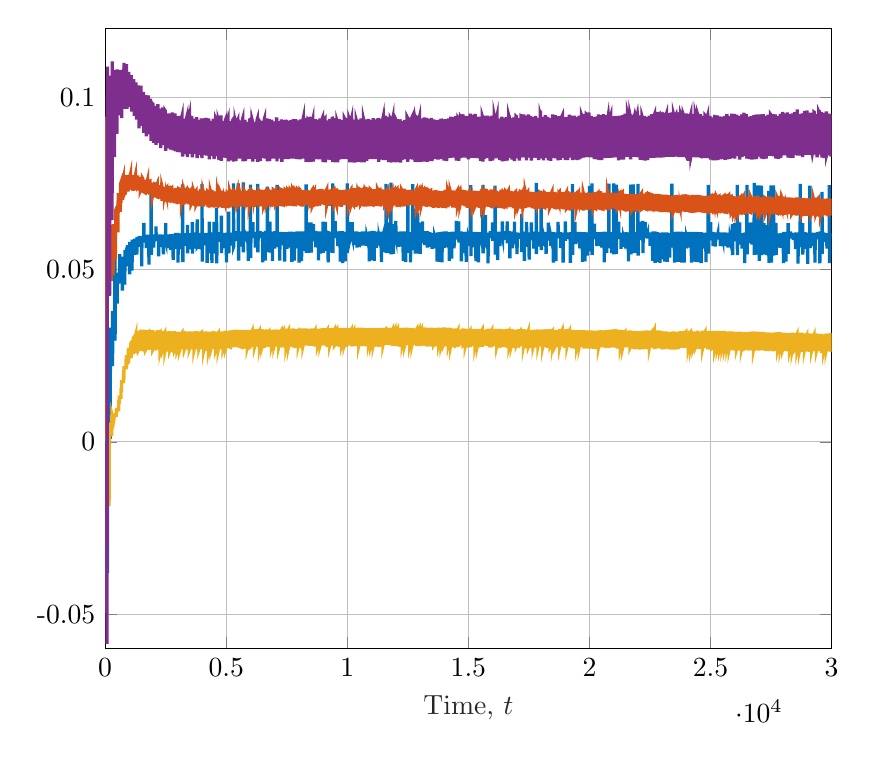
\begin{tikzpicture}

\begin{axis}[%
width=0.761\textwidth,
height=0.65\textwidth,
at={(0\textwidth,0\textwidth)},
scale only axis,
xmin=0,
xmax=30000,
xlabel style={font=\color{white!15!black}},
xlabel={Time, $t$},
ymin=-0.06,
ymax=0.12,
axis background/.style={fill=white},
xmajorgrids,
ymajorgrids,
ytick = {-0.05,0,...,0.1},yticklabels = {-0.05,0,...,0.1}
]
\addplot [color=mycolor1, line width=1.2pt, forget plot]
  table[row sep=crcr]{%
0	0\\
2.1429703121903	0.0444529173946648\\
7.62078471415589	-0.00166405148411286\\
10.2144458867369	0.0104451098050049\\
12.6935285233594	-0.0487898229475832\\
19.0024166006078	-0.0438260732807976\\
21.6341449197353	-0.0374827822561201\\
100.333621465626	-0.0374827822561201\\
103.15948508188	0.00684112435192219\\
108.841166682076	0.0191103428405768\\
111.689288870384	-0.0137503648766142\\
117.772474843459	-0.00234265529797995\\
120.968578818061	0.00764578379676095\\
199.809730362987	0.00764578379676095\\
202.101446071563	0.0331370041858463\\
208.472820728439	0.0249844619538635\\
211.539249661768	0.000894745891855564\\
216.010285187724	0.0203137844073353\\
219.836383353468	0.0224487998202676\\
300.392292997851	0.0224487964660511\\
305.003300725621	0.0380290638568113\\
310.101743421972	0.0257080430819769\\
313.797145832774	0.0338090098848625\\
319.831119357881	0.0320161837480555\\
399.566645949635	0.0320161839663342\\
401.596780873919	0.060644462620985\\
408.020542798851	0.0415521227150748\\
411.421409071962	0.0293547374931222\\
417.864423662864	0.0404840560404409\\
421.373701817352	0.0406190422036161\\
500.179081868777	0.0406190422036161\\
504.465917786518	0.0483139188363566\\
510.868257740993	0.0483659831261321\\
515.838572820398	0.0456903034901188\\
521.107462027088	0.0464990605250932\\
600.022212837772	0.0464990605250932\\
602.672500428936	0.0544963483989704\\
609.683483558674	0.0519526599164237\\
614.40414077344	0.0486120930363541\\
620.745964045225	0.0506635259771429\\
700.99915723093	0.0506634525954723\\
707.663192768276	0.0509701358532766\\
711.877846211777	0.0438879975881719\\
719.002974921601	0.051463936244545\\
723.524635392067	0.0532617458266031\\
800.631766607268	0.0532617458266031\\
806.437082491226	0.0536558479470841\\
811.710224354163	0.0455967175657861\\
818.729012973348	0.0533840219432022\\
822.584666089948	0.0552408110961551\\
899.139292986154	0.0552408110961551\\
901.158366548796	0.0565703618049156\\
908.32016420189	0.054977633033559\\
912.174388348241	0.0509539918093651\\
919.376237631674	0.0545969161357789\\
924.221934213645	0.0566395187524904\\
1000.23430368443	0.0566395187524904\\
1006.07411180477	0.0550563650103868\\
1011.37546106351	0.0485967017630173\\
1018.86337179198	0.0558765763707925\\
1022.94220741022	0.0575253603565216\\
1100.33923419331	0.0575253603565216\\
1107.0030412346	0.0550680696906056\\
1111.89815581251	0.0497058151049714\\
1119.026855753	0.0565162118255103\\
1123.41616845127	0.0581826725610881\\
1201.04010165581	0.0581824270884681\\
1208.17608103233	0.0542602743917087\\
1212.79840963939	0.0545637717150385\\
1219.90195438917	0.0584658953630424\\
1301.00872257466	0.0584658404623042\\
1307.86856223811	0.0543653086060658\\
1312.5064435382	0.055337446872727\\
1319.28165371157	0.0573046265963058\\
1323.10139945319	0.0589994982692588\\
1400.04246433743	0.0589994982692588\\
1404.07303538179	0.0565711993476725\\
1410.92555771356	0.0589228261560493\\
1417.00388599491	0.0573305442012497\\
1421.84138523702	0.0592831003523315\\
1500.31546345615	0.0592831003523315\\
1506.57312321335	0.0556755645375233\\
1511.70017968949	0.05090177983584\\
1518.91323295227	0.0579821397404885\\
1523.12325550624	0.0592633033702441\\
1599.31098655536	0.0592633033702441\\
1602.00031506891	0.0635394803284726\\
1609.35045759215	0.05873817356769\\
1613.99720654473	0.0578181513810705\\
1620.72318385332	0.0596158003754681\\
1700.00768153445	0.0596158003754681\\
1703.99491768923	0.0562244977809314\\
1710.79978572428	0.0592551173613174\\
1717.35573771788	0.05787949972364\\
1721.84952043256	0.0595570310179028\\
1800.38755582019	0.0595570310179028\\
1806.41727784988	0.0558757157559739\\
1811.65479226461	0.0514704016241012\\
1818.51036044772	0.0579054609224841\\
1822.91449497836	0.059674011230527\\
1898.96363793215	0.059674011230527\\
1901.47028032636	0.0742536572470271\\
1908.72673718709	0.0542958245277987\\
1913.0259732342	0.0565068393370893\\
1919.94303399767	0.0597546772223723\\
2000.09615430935	0.0597546772150963\\
2004.01552237243	0.0563766112536541\\
2010.91461357622	0.0591493652464123\\
2017.76379775714	0.0579122159542749\\
2022.21919173714	0.0596007186541101\\
2099.44551715182	0.0596007186541101\\
2102.17803504841	0.0625276726168522\\
2109.40262565545	0.0585001097933855\\
2114.47229342702	0.058281957240979\\
2120.87982604106	0.0596724243005156\\
2200.96223073833	0.059672426461475\\
2207.75954211497	0.0546887975469872\\
2212.16087281357	0.0538095581541711\\
2219.00298744309	0.05853830135311\\
2223.90773869195	0.0597410697519081\\
2300.03599674917	0.0597410697519081\\
2303.59603572766	0.0565234223140578\\
2310.41192036837	0.0591355836368166\\
2316.72818066891	0.0582047448297089\\
2321.61841416669	0.0596559122204781\\
2401.07666902033	0.0596569199442456\\
2408.11554898955	0.0544229692786757\\
2419.2687176402	0.0582607465221372\\
2424.17948257758	0.0595716853786143\\
2499.59257225718	0.0595716853786143\\
2502.26957796335	0.0634549772694299\\
2509.42201387088	0.0583373331501207\\
2513.68868346473	0.0581961674579361\\
2520.26243371515	0.0597107528810739\\
2600.17822822938	0.0597107528810739\\
2604.23456583952	0.0562027722080529\\
2610.80474267547	0.0591545155511994\\
2617.00310114247	0.0581892346745008\\
2621.67784858848	0.0596644326069509\\
2700.22368743401	0.0596644326069509\\
2705	0.0557114151961287\\
2711.03304725207	0.0591859797495999\\
2717.21980816186	0.058422210477147\\
2721.87048550599	0.0598273696014076\\
2801.00616986641	0.0598273430368863\\
2807.81016608424	0.0544556659733644\\
2812.13697770629	0.052791420781432\\
2818.81529683008	0.0586400174543087\\
2822.85324737299	0.059837316028279\\
2900.32062980273	0.059837316028279\\
2905.12459163023	0.0560031401946617\\
2911.09213270053	0.059367976798967\\
2917.0023110632	0.0587858599355968\\
2921.67787110436	0.0601322230177175\\
3000.97635245855	0.0601322250149678\\
3007.11068748392	0.0559598866529996\\
3011.61980768279	0.0520141776105447\\
3017.80283832515	0.0586653581522114\\
3021.84377109093	0.0599916467181174\\
3100.60097592597	0.0599916467181174\\
3106	0.0558577426854754\\
3111.06408725242	0.0592322042139131\\
3116.75234870506	0.0587148658414662\\
3121.10841696722	0.060043480789318\\
3199.53876804703	0.060043480789318\\
3201.58200613423	0.0747039190100622\\
3208.21759549175	0.0546229435130954\\
3212.09998145687	0.0521601911568723\\
3218.35630084	0.0585926449821272\\
3222.50141182421	0.0600668784391019\\
3300.27100750934	0.0600668784391019\\
3303.89632743043	0.0568480266192637\\
3309.92693583981	0.0592795622687845\\
3314.50315311764	0.0586904293522821\\
3320.40108355875	0.0601064309630601\\
3399.73811650526	0.0601064309630601\\
3402.17005041948	0.062989327183459\\
3409.00607541228	0.0547240881096513\\
3412.60160627479	0.0566308809320617\\
3419.20268224487	0.059055219644506\\
3423.52180546665	0.060104661341029\\
3500.90756517103	0.060104661341029\\
3506.09107654371	0.0558867949694104\\
3510.95060424976	0.0593397016709787\\
3516.7830118806	0.0589066150860162\\
3521.32582004987	0.0601142402265396\\
3599.76433193531	0.0601142402265396\\
3602.00046421414	0.0637226693397679\\
3608.80539905221	0.0546141144441208\\
3612.32217278336	0.0566612841212191\\
3618.77337773734	0.05910030035011\\
3622.96847715085	0.060268576566159\\
3700.25676763046	0.060268576566159\\
3704.81176309022	0.0560830358153908\\
3710.373441808	0.0592467090500577\\
3716	0.0588745858403854\\
3721.12245391358	0.0600435684245895\\
3799.45475128472	0.0600435684245895\\
3801.88664588235	0.0645263166916266\\
3808.47611844205	0.0566727832047036\\
3812.27498387385	0.0567118562976248\\
3818.79004336814	0.0591882214212092\\
3822.86987494929	0.0601790848595556\\
3900.58107172848	0.0601790848595556\\
3906.09052444064	0.0559153675640118\\
3910.90999239067	0.0593019196930982\\
3916.77079197533	0.0587637301832729\\
3921.46780069387	0.0600657502873219\\
3999.22527093806	0.0600657502873219\\
4001.6412796855	0.0747974830701423\\
4008.06822936338	0.054809702145576\\
4011.85783192968	0.0522787686932134\\
4018.79622438509	0.059106110376888\\
4023.03311907812	0.0601140495127765\\
4100.12651251736	0.0601140495127765\\
4103.33798392118	0.0569983583918656\\
4109.49806211522	0.0584377369013964\\
4113.36759002267	0.0586595131790091\\
4120.15878863379	0.0601841346651781\\
4201.00828223664	0.0601841161005723\\
4206.96064937193	0.0557264812923677\\
4211.28083809825	0.0519677639240399\\
4217.88772306601	0.0587238989755861\\
4222.00317048535	0.0601787776759011\\
4299.79615001412	0.0601787776759011\\
4302.42962516301	0.0639315340595203\\
4309.00323328197	0.0546762619487708\\
4312.827772976	0.0568660303943034\\
4319.77101667516	0.0602597556062392\\
4401.04979510924	0.0602578905782138\\
4406.92531620958	0.055760922277841\\
4411.35875606601	0.051964135174785\\
4417.73247370151	0.0587894731579581\\
4421.96696244987	0.0603276220899716\\
4499.92382164223	0.0603276220899716\\
4502.46974038226	0.0638525516333175\\
4509.0383319938	0.0546462863894703\\
4512.86138130377	0.0568864415727148\\
4519.74919159613	0.0601506975435768\\
4554.1199873136	0.0601614475890528\\
4598.41809816221	0.0601614475890528\\
4601.20230242138	0.0679592982814938\\
4607.35336408094	0.056462115397153\\
4611.7028994931	0.0518273939560459\\
4618.63882834279	0.0590551130080712\\
4622.92056691245	0.0601664296991657\\
4700.05895349855	0.0601664296991657\\
4703.00297335624	0.0608701663513784\\
4709.7177956034	0.0586175228345382\\
4714.1036375142	0.0585999214636104\\
4720.5708311624	0.0601675348880235\\
4799.32649120527	0.0601675348880235\\
4801.87033012637	0.0656334222148871\\
4808.19896336354	0.0547967055135814\\
4812.2553915837	0.0568734066218894\\
4819.1859545513	0.0591974656053935\\
4824	0.0601891324222379\\
4900.2036738031	0.0601891324222379\\
4904	0.0562221384861914\\
4910.55972756127	0.0592824533523526\\
4916.00330713585	0.0587643180842861\\
4921.24138306996	0.0601253971690312\\
5001.08920827833	0.0601289653423009\\
5007.00093248662	0.0558432257093955\\
5011.62899045114	0.0520607185681001\\
5018.37065311713	0.0586444010550622\\
5022.78953169446	0.0602394301786262\\
5099.44269328818	0.0602394301786262\\
5101.85813216299	0.0667726036408567\\
5108.74627681381	0.0546965104877017\\
5113.0343599325	0.056868292245781\\
5119.61561598695	0.0591489279977395\\
5124.91453528286	0.0602408752201882\\
5200.09754393623	0.0602408752201882\\
5203.39107991358	0.0569787010535947\\
5209.90839354102	0.0594719148066361\\
5216.24543602869	0.059033618101239\\
5221.25546140975	0.0601757541589905\\
5299.05031351838	0.0601757541589905\\
5301.76119009525	0.0749933436236461\\
5308.38793498067	0.0567132543073967\\
5312.45721138182	0.0567940376931801\\
5319.39422424302	0.0590677970540128\\
5323.80358989279	0.0602973338500306\\
5400.00465037261	0.0602973338500306\\
5402.94040406208	0.0611446850816719\\
5409.57733857635	0.0583293106828933\\
5415.01853605729	0.0588306596946495\\
5421.01659445115	0.0602148587131524\\
5498.68336567403	0.0602148587131524\\
5501.31513854385	0.0749645737996616\\
5507.64115087972	0.0545755210332572\\
5512.00259568214	0.0525798578382819\\
5519.11966067024	0.0593358179939969\\
5523.70358735287	0.0602877940400504\\
5600.16846527309	0.0602877940400504\\
5603.99406115813	0.0566752089798683\\
5610.68720598689	0.0596831216753344\\
5616.40172690298	0.059371468880272\\
5621.30468205311	0.0605756556578854\\
5698.87197904504	0.0605756556578854\\
5701.49643807469	0.0752568235839135\\
5707.95140895514	0.0549768106939155\\
5712.34631878633	0.0571262673438468\\
5719.25690120571	0.059579673645203\\
5724.01079269244	0.0605350099867792\\
5800.02620666274	0.0605350099867792\\
5803.16836398749	0.0590611610496126\\
5810.0902202252	0.0595834811174427\\
5816.15466093113	0.0594530316157034\\
5821.20237459952	0.0606006525740668\\
5900.57302015483	0.0606006525740668\\
5906.03352886621	0.0562063214856607\\
5911.36837063429	0.0525464051606832\\
5918.31740858835	0.0590968139767938\\
5922.29971056307	0.0604788213058782\\
5998.44317113341	0.0604788213058782\\
6001.28091168779	0.0746640877441678\\
6007.30525959839	0.0562076109818008\\
6012.1447243853	0.0533259471885685\\
6019.48390221954	0.0591252777412592\\
6023.66153655049	0.0603031164428103\\
6099.84330365066	0.0603031164428103\\
6102.73821172836	0.0637873366067652\\
6109.81703562	0.0595755238282436\\
6116.00344287793	0.0591429860796779\\
6121.31178211188	0.0604596211414901\\
6200.36119534459	0.0604596211414901\\
6204.90446631811	0.0563416746008443\\
6211.20663823303	0.0581848752772203\\
6217.96814702838	0.0589824373855663\\
6221.95219968908	0.060361119270965\\
6298.92121391828	0.060361119270965\\
6301.74131383836	0.074864019479719\\
6308.03466253577	0.0549735331587726\\
6312.5066002795	0.0568310805865622\\
6319.37901766381	0.0591678229357058\\
6323.70196727631	0.0604881895415019\\
6400.01675392055	0.0604881895415019\\
6403.06486042093	0.0611420072382316\\
6409.82125192486	0.0595754885944189\\
6416	0.0591272590972949\\
6421.03520784756	0.0604530619893922\\
6500.99853838913	0.0604530586788314\\
6506.15608149153	0.0560626607111772\\
6511.59897689697	0.0521203515600064\\
6518.78988490175	0.0593333130018436\\
6522.80401087968	0.0603209758555749\\
6601	0.0603209735672863\\
6606.32381643127	0.0561971503520908\\
6611.50849228444	0.0525815549372055\\
6618.48839260461	0.0591160865478741\\
6622.3109266533	0.0607135284517426\\
6699.03757205565	0.0607135284517426\\
6701.79333817863	0.0740239331680641\\
6708.02877695638	0.0550331534104771\\
6712.83703166357	0.0570597765072307\\
6719.76658393868	0.0604938334217877\\
6799.766267969	0.0604946701168956\\
6802.60430172021	0.0639291749757831\\
6809.10110935699	0.0549284503977105\\
6813.93890827283	0.0590132836041448\\
6820.65066362805	0.0605521007855714\\
6900.78910660546	0.0605521007855714\\
6906.60931277213	0.0559909545809205\\
6911.94791900303	0.0525412763709028\\
6919.20963844111	0.0594226846151287\\
6923.379271279	0.060377337726095\\
7000.49159079201	0.060377337726095\\
7005.51132393699	0.0561015169041639\\
7011.17432801952	0.0611114924977301\\
7017.82212516034	0.0589176050270908\\
7021.96836690782	0.0605589965925901\\
7098.90576444144	0.0605589965925901\\
7101.78097701937	0.0745456069125794\\
7108.51371387645	0.0565411234492785\\
7112.83159545859	0.0570031028182711\\
7119.94133429677	0.0603000436312868\\
7200.80615014064	0.0603000440351025\\
7206.82191335597	0.0559417025324365\\
7211.84057310519	0.0526227008740534\\
7218.90304704746	0.0594934109140013\\
7222.95844435946	0.0604534957747092\\
7300.06976957812	0.0604534957747092\\
7303.55596093882	0.0570107047824422\\
7310.89411168927	0.0596166462928522\\
7317.74168893769	0.0589941477119282\\
7322.02083579929	0.0603283629643556\\
7400.35230068004	0.0603283629643556\\
7405.56431418971	0.056193520045781\\
7411.45992800876	0.052300382310932\\
7418.66171495996	0.0594238445519295\\
7423	0.0604012890362355\\
7500.21980586554	0.0604012890362355\\
7504.95365737511	0.0560354782319337\\
7511.10644291727	0.0591290188131097\\
7518.02819805711	0.0590362700932019\\
7522.62782458097	0.06036163922181\\
7600.2231707924	0.06036163922181\\
7604.50702968773	0.0563876297746901\\
7611.14388079901	0.0599197881601867\\
7618.07684123344	0.0591160976691754\\
7622.43093867413	0.0605508982662286\\
7700.24178057159	0.0605508982662286\\
7704.57106112706	0.0562791652555461\\
7711.36595432442	0.0522311017084576\\
7718.31165196934	0.0589790980411635\\
7722.48067772292	0.0601469750181423\\
7800.24649635406	0.0601469750181423\\
7805.00168651426	0.0560524252578034\\
7811.363958547	0.0525753449910553\\
7818.21146411587	0.0591958795230312\\
7822.36746542379	0.0604808129864978\\
7900.26103655685	0.0604808129864978\\
7905.23476009957	0.0561621802917216\\
7911.15567496596	0.060523362531967\\
7918.20892673814	0.059258131779643\\
7922.14401669169	0.0605866543846787\\
8000.22376746334	0.0605866543846787\\
8005.00357152856	0.0561329297597695\\
8011.37958121969	0.0519952703471063\\
8018.32637881931	0.0587315126067551\\
8022.66003553199	0.0605833699883078\\
8100.60524808175	0.0605833699883078\\
8106.15599899262	0.0560475246493297\\
8111.82982684387	0.0524443869326205\\
8119.00540560564	0.0595349039031134\\
8123.57372794385	0.06055148681844\\
8201.1083500383	0.0605709972951445\\
8207.58549115398	0.0553925832937239\\
8219.30792094637	0.0592983897513477\\
8224.0107818683	0.060433713846578\\
8299.00108942791	0.060433713846578\\
8301.46081095875	0.0746932413167087\\
8308.16728886086	0.0548187784879701\\
8312.91868559702	0.0573417738632997\\
8319.84077140761	0.0604716958659992\\
8399.15799812186	0.0604706845952023\\
8402.12432374022	0.0636959811236011\\
8409.12535196123	0.0548645036687958\\
8413.88488230548	0.0590190628245182\\
8420.58818214518	0.0605183821171522\\
8499.23118380304	0.0605183821171522\\
8502	0.063704643795063\\
8509.11161281365	0.0549007057634299\\
8513.8068227381	0.0591432101828104\\
8520.63468746386	0.0606487269542413\\
8599.83785553707	0.0606487269542413\\
8602.83978563934	0.0632163324626163\\
8609.73083100461	0.0593592075674678\\
8616.00812510806	0.0592547447813558\\
8621.11046731657	0.0607640214802814\\
8700.17749462817	0.0607640214802814\\
8704.32796672887	0.0564404708129587\\
8711.13680572374	0.0599518592971435\\
8718.20364225956	0.0591692063717346\\
8722.37942672898	0.0604921226258739\\
8801.03385755087	0.0604920751102327\\
8807.44856303841	0.0565789854445029\\
8811.89405545056	0.0526318908232497\\
8818.94943810649	0.0595642441512609\\
8823.00279289713	0.0606201874506951\\
8898.04577280114	0.0606201874506951\\
8901.1438055781	0.0610385937834508\\
8907.64636194746	0.0546391297320952\\
8912.56751240066	0.0571442191139795\\
8919.57817039848	0.0593996565257839\\
8924.55475479965	0.060622059932939\\
8999.08315463386	0.060622059932939\\
9002.06200286057	0.0639181899969117\\
9009.09745142378	0.0548228875813948\\
9013.85416619627	0.0590737578677363\\
9020.31689901867	0.0606919057572668\\
9099.38459088326	0.0606919057572668\\
9102.2623856697	0.0638372977118706\\
9109.25346277159	0.0553328131063608\\
9114.23414617582	0.0592947322256805\\
9121.01195749822	0.0607061687296664\\
9200.21619845809	0.0607061687296664\\
9205.38868792813	0.056447314684192\\
9211.34540056573	0.052121921122307\\
9218.10104402562	0.0590180158287694\\
9222.28315232696	0.0604890353752126\\
9300.98023405882	0.0604890395989059\\
9307.94586807533	0.0549017659286619\\
9312.18416479052	0.0560700576061208\\
9319.39676106293	0.0592089417732495\\
9324.01617231996	0.0604072346977773\\
9398.88373069541	0.0604072346977773\\
9401.74109438606	0.0749946417417959\\
9408.78820662941	0.0547623559687054\\
9413.26448421547	0.0591253964812495\\
9420.16745903611	0.0605390322634776\\
9499.65304224574	0.0605390322634776\\
9502.67914040968	0.0640365060207841\\
9509.82653344512	0.0595929347946367\\
9516.0050167573	0.0591298862673284\\
9521.13500243677	0.0603930117795244\\
9600.06136319877	0.0603930117795244\\
9604.1936373999	0.0568238949854276\\
9611.00210632049	0.0595182318938896\\
9617.84090973267	0.0591046343870403\\
9622.25609885117	0.0605992994751432\\
9700.24712541403	0.0605992994751432\\
9706.00272807984	0.0561555909080198\\
9711.63550211257	0.0522806361950643\\
9718.66945893182	0.0597014631603088\\
9722.90574862199	0.0606670718334499\\
9800.24803182395	0.0606670718334499\\
9806.13883715562	0.0562051942033577\\
9811.74699103655	0.0518621718911163\\
9819.00731595695	0.0593258365006477\\
9823.69876039937	0.0603020426860894\\
9901.05845982456	0.0603020539747376\\
9907.30263716245	0.0560219879625947\\
9912.02825749792	0.0523694639123278\\
9919.0018741043	0.0593677273318463\\
9923.49170991523	0.0604710894695017\\
9998.46804490194	0.0604710894695017\\
10001.4469084635	0.0749772257222503\\
10008.2182446567	0.0548168948153034\\
10013	0.0568982745535322\\
10020.0194857839	0.0603428464419267\\
10099.1175324579	0.0603428464419267\\
10102.2521387552	0.0638099646785122\\
10109.3785886657	0.0587987658836937\\
10114.368363666	0.0589599586928671\\
10120.7545853081	0.0602078166375577\\
10199.5868475063	0.0602078166375577\\
10202.6865864142	0.063724099414685\\
10209.7321467284	0.0591309135706979\\
10215.0306919786	0.0589719994131883\\
10221.0722074346	0.0603808704618132\\
10299.9299193086	0.0603808704618132\\
10303.254454389	0.057074155407463\\
10309.9733818005	0.0592934193409747\\
10316.1556153589	0.0593084698739403\\
10321.3919837539	0.0605902373608842\\
10400.0828070248	0.0605902373608842\\
10404.0007312111	0.0563476155402896\\
10410.8980558425	0.0592968481614662\\
10417.7469963724	0.0589795372980007\\
10421.8979925171	0.0603685106361809\\
10500.0827706403	0.0603685106361809\\
10504.2163859805	0.0564771129247674\\
10510.9370507142	0.0594306401944777\\
10517.8095238806	0.0590722181841556\\
10521.8756597165	0.060301324872853\\
10599.9665657153	0.060301324872853\\
10603.7125281156	0.056922467010736\\
10610.6625766366	0.0592984014983813\\
10617.1220772062	0.0593232955179701\\
10621.813189233	0.0606034348311368\\
10700.0052095914	0.0606034348311368\\
10703.3945425233	0.0569627508702979\\
10710.6673669835	0.0594304057121917\\
10717.6455512177	0.0589608716327348\\
10721.8473445434	0.0604713927714329\\
10800.0176197393	0.0604713927714329\\
10803.8465420342	0.0568454103304248\\
10811.0009247094	0.0592473938158946\\
10817.8071365345	0.0590238907716412\\
10821.9101985973	0.0603693794728315\\
10900.4737027564	0.0603693794728315\\
10906.702837593	0.055797126791731\\
10912	0.0523909249095595\\
10919.0838120652	0.0594908319908427\\
10923.4651077885	0.0606285720132291\\
11000.2913712316	0.0606285720132291\\
11006.8109093863	0.0557367505098227\\
11011.8255899672	0.0527277754408715\\
11018.9067163453	0.0595358945756743\\
11023.0015050583	0.0607133941120992\\
11100.4245644205	0.0607133941120992\\
11107.0052996799	0.0558541598438751\\
11112.0420954932	0.0525468010127952\\
11119.2256526513	0.0595333694691362\\
11123.140673468	0.0604862750333268\\
11200.1029072544	0.0604862750333268\\
11204.4158321716	0.0562744866110734\\
11211.0826599137	0.0594979692432389\\
11217.6944235344	0.0592153998586582\\
11222.0006662482	0.0605248587598908\\
11299.8991022649	0.0605248587598908\\
11303.2773680307	0.0569437955346075\\
11310.511371376	0.0594118333538063\\
11317	0.0591912791060167\\
11321.7820358563	0.060476492253656\\
11400.198189729	0.060476492253656\\
11405.2674250216	0.0561976676690392\\
11411.2684254051	0.0521926758156042\\
11418.3780818856	0.0588291905878577\\
11422.7903450443	0.0605483437575458\\
11498.0863699353	0.0605483437575458\\
11501.1230598211	0.0606262706787675\\
11508.2444622319	0.0550522838530014\\
11512.86258452	0.0571464872591605\\
11519.7666514462	0.0603994340999634\\
11541.741299965	0.0603809205713333\\
11598.7463359547	0.0603809205713333\\
11601.5541440252	0.0748397140050656\\
11608.8877882458	0.0547405896577402\\
11613.7156802243	0.0588070096855517\\
11620.0382265582	0.0602869811482378\\
11699.0129974939	0.0602869811482378\\
11702	0.0637011907383567\\
11708.9672882705	0.0548010103557317\\
11713.3640344154	0.0590215920310584\\
11720.022167838	0.0604932467467734\\
11798.8906575859	0.0604932467467734\\
11801.7357606207	0.0751816323645471\\
11809	0.0544172626796353\\
11813.3432905831	0.0591189010301605\\
11820.5812182303	0.0606274261008366\\
11899.2336132048	0.0606274261008366\\
11902.2116097898	0.0631811865277996\\
11909.1591678833	0.0545860747879487\\
11914.0275645939	0.0591955526069796\\
11920.895694693	0.0604374225840729\\
11999.4021023297	0.0604374225840729\\
12002.6038234643	0.0641069004304882\\
12009.7742534167	0.0592830452333146\\
12015.4737326088	0.0590654389925476\\
12021.2317557584	0.0603488633496454\\
12099.9879825718	0.0603488633496454\\
12104.003612461	0.0565648017145577\\
12110.9882538098	0.0594497825186409\\
12117.1485798951	0.0591985014361853\\
12121.8236670084	0.060546564804099\\
12200.0657617887	0.060546564804099\\
12204.0040208578	0.0566632114241656\\
12211.047463712	0.0595601015666034\\
12217.8495290251	0.0591747406942886\\
12222.0661416632	0.0606262607725512\\
12300.1415868766	0.0606262607725512\\
12304.7177617048	0.056381209527899\\
12311.260034175	0.0524887546125683\\
12318.1439122822	0.0590189845679561\\
12322.298821744	0.0605575457921077\\
12400.2404598205	0.0605575457921077\\
12411.8395836354	0.0521451310305565\\
12419.0131283113	0.0594071770683513\\
12423.7157835886	0.0605200838945166\\
12499.013128978	0.0605200838945166\\
12501.8252985168	0.0714371711874264\\
12509	0.0548239878007735\\
12513.0716531289	0.0569825556558499\\
12520	0.0604112582732341\\
12600.6279882013	0.0604112582732341\\
12606.7421067926	0.0556347623532929\\
12611.6848720828	0.0520753992423124\\
12618.9526838496	0.0594042189659376\\
12623.2005594161	0.0603039045126934\\
12698.1580806361	0.0603039045126934\\
12701.2693654224	0.0747521864250302\\
12708.2853304137	0.0556266004205099\\
12712.8441126772	0.056983219794347\\
12719.9332388402	0.0603883738585864\\
12798.9696406794	0.060388373593014\\
12801.849409153	0.0676208710901847\\
12809.129660732	0.0545897394258645\\
12813.9527861309	0.0591392140449898\\
12820.4174871412	0.0605045095071546\\
12899.0335774478	0.0605045095071546\\
12901.8578655095	0.0665019501138886\\
12909.1571606482	0.0546455778057862\\
12914.074033342	0.0588731946227199\\
12920.6673582849	0.0603409766081313\\
12999.1254901689	0.0603409766081313\\
13001.9869624627	0.0636220961532672\\
13009.107826207	0.0545708397112321\\
13014.1528811463	0.058918471531797\\
13020.7216412418	0.060458868072601\\
13099.5035212114	0.060458868072601\\
13102.4272412565	0.0639563895601896\\
13109.6419212047	0.057626199137303\\
13115.0188380288	0.0593440181291953\\
13121.1321852457	0.0606053462033742\\
13199.9351652237	0.0606053462033742\\
13203.2612559777	0.0570615379510855\\
13210.698692775	0.0594613610155648\\
13217	0.0594761991560517\\
13221.5901071449	0.0606651447342301\\
13300	0.0606651447342301\\
13304.001238539	0.0563804679804889\\
13310.7995128483	0.0594480156469217\\
13317.3150404898	0.05917088703427\\
13321.8077830114	0.0603721909210435\\
13400.0017705594	0.0603721909210435\\
13403.5630118391	0.056617747330165\\
13410.7296126246	0.0590035465538676\\
13417.012313751	0.0589740559844358\\
13421.6388809554	0.060188163388375\\
13500.0862689867	0.060188163388375\\
13504.4301540957	0.055985682807659\\
13511.085388657	0.0590607991507568\\
13517.7292969227	0.0587793828017311\\
13522	0.0601676585174573\\
13600.1261785873	0.0601676585174573\\
13604.2479990393	0.0561263581439562\\
13610.9583394952	0.0592210464710661\\
13617.5251251206	0.0590398760468815\\
13622.1005350329	0.0601693661883473\\
13700.1275893873	0.0601693661883473\\
13705.005472771	0.0558903786950395\\
13711.2552150563	0.0522970132042246\\
13718.0029903344	0.0588010922183457\\
13722.0503271158	0.0602884742402239\\
13800.2207272848	0.0602884742402239\\
13811.5232524682	0.0522686481381243\\
13818.2368269386	0.0589808374279528\\
13822.8124934388	0.0603877016292245\\
13900.2420825786	0.0603877016292245\\
13906.0034097623	0.0559478644245246\\
13911.4783050408	0.052056769378396\\
13918.2590717105	0.0589741478179349\\
13922.8276329659	0.0605269140396558\\
14000.0971369568	0.0605269140396558\\
14004.4789693728	0.0563184638558596\\
14011.0299033817	0.0595264489056717\\
14017.6155288969	0.05923759624784\\
14022.04662243	0.0605652123376785\\
14100.0388308415	0.0605652123376785\\
14104.3232680285	0.0564179962530034\\
14111	0.0596380450842844\\
14117.4025860862	0.0592003038473194\\
14122.007407639	0.0602666667946323\\
14200.4363551548	0.0602666667946323\\
14207	0.0557200926014048\\
14211.8801706693	0.052495242052828\\
14218.7883803921	0.059418989050755\\
14223.0010463793	0.0603837858543557\\
14300.1914119351	0.0603837858543557\\
14305.1182335678	0.0560118531320768\\
14311.2434000097	0.0531557137874188\\
14318.1848710732	0.0590377941043698\\
14322.2715660404	0.0605020558068645\\
14400.134576652	0.0605020558068645\\
14405.016691792	0.0561332468532783\\
14411.2143286201	0.0570219511610048\\
14418.0820334978	0.0589990351145389\\
14422.1548438416	0.0604527451469039\\
14499.6386989575	0.0604527451469039\\
14502.3223953782	0.064132963794691\\
14509.461111458	0.0586909009543888\\
14514.6692121638	0.0593006194576446\\
14520.7991929907	0.0605710055060626\\
14599.1994502321	0.0605710055060626\\
14602.2877718327	0.0639849060935376\\
14609.6268818932	0.0578274272484123\\
14614.4550288233	0.0591304933404899\\
14620.7415757754	0.0606231277051847\\
14700.9675305408	0.06062312818176\\
14707.8336156739	0.0548166290100198\\
14712.1065911313	0.052365316907526\\
14719.2312386635	0.0593367034416588\\
14724.1540419168	0.0604048192617483\\
14801.1052867825	0.0604215694365848\\
14808.2073787449	0.0547687258913356\\
14812.5274020585	0.0570026641908044\\
14819.4862549718	0.059300961340341\\
14824.3324313056	0.0604207981741638\\
14900.2015896012	0.0604207981741638\\
14905.0368084926	0.0559248445606499\\
14911.3331951652	0.052211359856301\\
14918.2099424028	0.0590207961504348\\
14922.3395962365	0.0605071094541927\\
14999.9313557208	0.0605071094541927\\
15003.2712750303	0.0569062454451341\\
15010.2027667905	0.0593452065695601\\
15016.0915212915	0.0592038856739237\\
15021.2371223803	0.0606002192762389\\
15098.2206585795	0.0606002192762389\\
15101.2563841964	0.074522333972709\\
15108.6899505936	0.0539000579192361\\
15112.865880749	0.0572880421023001\\
15119.8504708835	0.0603764464794949\\
15201.0526480486	0.060376415054634\\
15208.4115069694	0.0564665086239984\\
15212.721015343	0.0570930923095148\\
15219.5707409121	0.0593690057758067\\
15224.7680535497	0.0604497342428658\\
15300.6967496248	0.0604497342428658\\
15307.2757973144	0.0561426843378285\\
15312.0837744774	0.0524635006186145\\
15319.0840737112	0.0593853165264591\\
15323.5238095764	0.0603826208207465\\
15400.2306859085	0.0603826208207465\\
15406	0.055947954126168\\
15411.6198684649	0.052074661522056\\
15418.6925765998	0.0593626649279031\\
15422.746309463	0.0602589294903737\\
15499.8293715802	0.0602589294903737\\
15503	0.0606117320858175\\
15510.0037458045	0.0593602360786463\\
15516.122208202	0.0591434791676875\\
15521.0587330851	0.0604081390047213\\
15598.8631357176	0.0604081390047213\\
15601.7597330041	0.0745694575125526\\
15609.1412357822	0.0546631222787255\\
15613.9262091042	0.0589912160648964\\
15620.1891888877	0.0601295408450824\\
15698.0277224685	0.0601295408450824\\
15701.1920413883	0.0657751602375356\\
15708.4524200534	0.0563556454435457\\
15712.9139883449	0.0571389046781405\\
15719.9470970476	0.0602099114839802\\
15800.7915551774	0.0602099114839802\\
15807.0843917138	0.0554718098028388\\
15811.7789118478	0.0517620864848141\\
15818.6945268962	0.0591498993780988\\
15822.8707243284	0.0602409657985845\\
15899.8854023559	0.0602409657985845\\
15902.9139977005	0.06112015585677\\
15910.0226005166	0.0593820018657425\\
15916.0735731303	0.0590811898509855\\
15921.2040183493	0.0603896044449357\\
15999.073904802	0.0603896044449357\\
16001.9905210474	0.0636673428198264\\
16009.562842836	0.0583171034122643\\
16014.9664055401	0.0590050380160392\\
16020.9591268934	0.060279534849542\\
16098.4739697764	0.060279534849542\\
16101.570869467	0.0743736023432575\\
16108.7449528564	0.0543264588377497\\
16113	0.0572345617001702\\
16119.8630045396	0.060358155205904\\
16200.9183040391	0.0603581707509875\\
16207.6191416823	0.0547117082205659\\
16212	0.0527235602748988\\
16218.9248049008	0.0596850471702055\\
16223	0.0605350035948504\\
16300.0958851931	0.0605350035948504\\
16304.0451058638	0.0568022084589757\\
16310.8075224382	0.0595380947706872\\
16317	0.0592596786700597\\
16321.5897547781	0.0605120029722457\\
16399.3889118737	0.0605120029722457\\
16402.7531872011	0.0639971809614508\\
16409.9888665238	0.059505674020329\\
16416.055977529	0.0592687633543392\\
16421.2790418804	0.0605230191613373\\
16503.1191194867	0.0605572092536022\\
16510.6274417888	0.0591897231824987\\
16517.1029741897	0.0592168891562324\\
16521.7845175002	0.0606653942304547\\
16599.3543609293	0.0606653942304547\\
16602.364500253	0.0639626315314672\\
16609.6377233958	0.0575876042457821\\
16614.3327786116	0.0590681962239614\\
16620.7403232098	0.0606388331798371\\
16701	0.0606388357846299\\
16707.9572428495	0.0547588078807166\\
16712.1383532482	0.0532421936150058\\
16719.2520929173	0.0594064814467856\\
16723.9785046391	0.060497047361423\\
16800.1036993212	0.060497047361423\\
16804.8042018444	0.0561844856856624\\
16811.1481606547	0.0601157560413412\\
16818	0.0589542127927416\\
16822.3036598085	0.0604081456440326\\
16899.6042104994	0.0604081456440326\\
16902.712928355	0.0639303986245068\\
16910	0.0591579169922625\\
16916	0.0589803529474011\\
16921.23084597	0.0602972821543517\\
17000.9359542796	0.0602972821288859\\
17007.7611073177	0.054510428730282\\
17012.2574798937	0.05691855796249\\
17019.4231545639	0.0590001899290655\\
17024.4010446041	0.060227463618503\\
17099.8487918001	0.060227463618503\\
17103	0.0604797454216168\\
17110.002156114	0.0592442426350317\\
17116	0.0588508543842181\\
17121.2799671293	0.0601539416384185\\
17198.8151458541	0.0601539416384185\\
17201.860253167	0.0661578655053745\\
17209.2610405919	0.0550318107161729\\
17213.8582653826	0.0589053815019724\\
17220.4158288358	0.0605047282697342\\
17300.4789167275	0.0605047282697342\\
17307.0012565441	0.0558182535714877\\
17311.829816216	0.0525110091220995\\
17318.9873781247	0.0594839774712455\\
17323.2853100893	0.0604676640214166\\
17399.234425079	0.0604676640214166\\
17402.0322664219	0.0638431044681056\\
17409.287486069	0.0565816773196275\\
17414.3295416211	0.0589913128133048\\
17420.7672626332	0.0603133841432282\\
17500.8290140776	0.0603133841432282\\
17507.6480097346	0.0544019286862749\\
17512.1350337437	0.0528594569295819\\
17519.1832680543	0.059175127553317\\
17523.9656333788	0.060190168551344\\
17599.1596261768	0.060190168551344\\
17602.0598753486	0.0636574702803046\\
17609.4367500463	0.0584652695033583\\
17613.9003658528	0.0589573974284576\\
17620.2908069849	0.0604422697251721\\
17700.1830445601	0.0604422697251721\\
17705.0016602568	0.0560871974630572\\
17711.183013297	0.0610062302839651\\
17718.1629153161	0.0590860999764118\\
17722.3358678995	0.0603438338948763\\
17798.7188753573	0.0603438338948763\\
17801.6175667274	0.0751196422643261\\
17809	0.0544568118966708\\
17813	0.0572138346324209\\
17819.8853370134	0.0602630635985406\\
17900.0723401864	0.0602630634020898\\
17903.8011284756	0.0566352941277728\\
17910.4201596896	0.0592977404412522\\
17916.3250388274	0.058943856802216\\
17921.4532267201	0.0604446952675062\\
17998.0384902536	0.0604446952675062\\
18001.2300902852	0.0728189722321986\\
18008.2826141349	0.0556270994675288\\
18012.7400109835	0.0569317191111622\\
18019.6911577901	0.0602236813429045\\
18024.7182041462	0.0604604905201995\\
18100.0475541204	0.0604604905201995\\
18103.8751503986	0.0568757271612412\\
18110.7950694817	0.0594786130131979\\
18117.3576197058	0.0592715741113352\\
18121.8558473103	0.0604478321220085\\
18201.0810518611	0.0604490134610387\\
18208	0.0545300170342671\\
18212.3353807029	0.0566503813934105\\
18219.6466058066	0.0598572585586226\\
18224.8233668846	0.0602080102653417\\
18299.6916677701	0.0602080102653417\\
18302.6355253019	0.0636323843646096\\
18309.3931048187	0.0583815400168533\\
18314.1026714543	0.0587768511977629\\
18320.4323670075	0.0604370096370985\\
18400	0.0604370096370985\\
18403.3886275521	0.056852264340705\\
18409.995766234	0.059312486431736\\
18415.9745591531	0.0590967552525399\\
18421.213794656	0.0604406969687261\\
18500.2132367286	0.0604406969687261\\
18505.6407456067	0.0558693692582892\\
18511.3102030261	0.0520215425422066\\
18518.1015782541	0.0588221591060574\\
18522.5197379783	0.0603384346359235\\
18600.5683646314	0.0603384346359235\\
18607.1587594198	0.0557073613526882\\
18612	0.0524402984374319\\
18618.9926748141	0.0594461158470949\\
18623.3463380954	0.0602792125209817\\
18699.553921737	0.0602792125209817\\
18702.6063623789	0.0638248488721729\\
18709.843838759	0.0593795288550609\\
18715.8335373007	0.0591220075912133\\
18721.1861742546	0.0604299064798397\\
18800.0942885196	0.0604299064798397\\
18804.385791057	0.0562270036061818\\
18811.0400135207	0.0592882558230485\\
18818	0.0589436008522171\\
18822.1331713094	0.0602613700066286\\
18900.63250073	0.0602613700066286\\
18907.3425437036	0.0562778806743154\\
18912.0924635319	0.0520038517752255\\
18919.1911564474	0.0592270719425869\\
18923.6612493689	0.0601847220787022\\
18999.3577303734	0.0601847220787022\\
19002.338042577	0.0639647962198069\\
19009.4464948826	0.0583132279825804\\
19014.2909076114	0.0589034962540609\\
19020.6306887121	0.0602585480664857\\
19099.8085220013	0.0602585480664857\\
19103.1195967416	0.0600031168360147\\
19110.56699753	0.0592909749684623\\
19117.1436643781	0.0589599898739834\\
19121.7852832871	0.0602766883421282\\
19200.2564171248	0.0602766883421282\\
19206.090962844	0.0558048013117514\\
19211.5110665874	0.0519526366661012\\
19218.2281526694	0.0588125801514252\\
19222.3961737128	0.0603757438984758\\
19299	0.0603757438984758\\
19301.6342295443	0.0747741337982006\\
19309	0.0542817267923965\\
19313.2998701373	0.0587855515914271\\
19320.012880577	0.0603743946630857\\
19399.1643357143	0.0603743946630857\\
19402.2514721717	0.0637749472662108\\
19409.6494718305	0.0573744073335547\\
19414.3672070673	0.058951154944225\\
19421	0.0603656759267324\\
19499.8304084676	0.0603656759267324\\
19502.983070966	0.0606178300913598\\
19510.0036527544	0.059227763889794\\
19516	0.0590831111767329\\
19521.1718718575	0.0604662339646893\\
19600.101289704	0.0604662339646893\\
19604.9206082047	0.0561587760057591\\
19611.003101545	0.0594144925707951\\
19617.6882551574	0.058908986960887\\
19621.9003575912	0.0603323664799973\\
19700.8264074102	0.0603323664799973\\
19707.5286336341	0.0562097458423523\\
19712.0198919338	0.0522590572400077\\
19719	0.0593073479831219\\
19723.0836157958	0.0603522282326594\\
19800.8394991588	0.0603522282326594\\
19807.4126782584	0.0564508690549701\\
19812.0489227728	0.0523579739892739\\
19819.0791494442	0.059266361513437\\
19823.42078795	0.0602965101752488\\
19900.9623139712	0.0602965096550179\\
19907.8884241523	0.0546573555257055\\
19912.1612693987	0.0540325193833269\\
19919.2893385545	0.0589122212913935\\
19924	0.0601628962867835\\
19998.168861338	0.0601628962867835\\
20001.2756167366	0.0742732401558897\\
20008.2638412028	0.0552824517908448\\
20012.8463445257	0.056816482290742\\
20019.72201125	0.0602060775891005\\
20024.4599634979	0.0602973095301422\\
20098.3787092719	0.0602973095301422\\
20101.3747830293	0.0749756715886178\\
20108.7262291444	0.0542867746444244\\
20112.8350264264	0.0568342881488206\\
20119.7513143262	0.0602433020430908\\
20199.7120571567	0.0602406550679007\\
20202.8116678192	0.0633131221256917\\
20210	0.059402054608654\\
20215.9730688005	0.0587669647939038\\
20221.1732766805	0.0602589529371471\\
20299.928713746	0.0602589529371471\\
20303.2604972032	0.0567840491712559\\
20310.6617747763	0.0591782323353982\\
20317.0123180531	0.0589289320814714\\
20321.6507854216	0.0603653111647873\\
20400.0019172294	0.0603653111647873\\
20404.0687046786	0.0568061123522057\\
20411.0014743868	0.0592381930073316\\
20417.3234978122	0.0589506183641788\\
20421.7959707443	0.0602402848744532\\
20500.0307271322	0.0602402848744532\\
20504	0.0563573893159628\\
20510.8215175669	0.0594435222483298\\
20517.0482848641	0.0589958512755402\\
20521.6597619186	0.0604272322088946\\
20600.29921119	0.0604272322088946\\
20606.8141711707	0.0557507719058776\\
20611.6192997745	0.0520835278512095\\
20618.9290415622	0.0595542504051991\\
20623.0208987984	0.0605093393860443\\
20698.0042884813	0.0605093393860443\\
20701.140224159	0.0608384131264756\\
20708.2123524551	0.054810469642689\\
20712.4750198401	0.0565329389210092\\
20719.4474220272	0.058940832834196\\
20724.1540469404	0.0602208322598017\\
20798.1091965925	0.0602208322598017\\
20801.2644698655	0.074888559684041\\
20808.4819116854	0.0561910658871057\\
20812.8011709668	0.056829260494851\\
20819.7203654893	0.0602452937964699\\
20824.978004006	0.060375811666745\\
20901.0183769125	0.0603758081306296\\
20908.036873441	0.0547786414826987\\
20912.2096368255	0.0569563564276905\\
20919.3044360811	0.0590342451541801\\
20924.3683314021	0.0602863416715991\\
20998.7898140864	0.0602863416715991\\
21001.5476089922	0.0749916646782367\\
21008.8116810477	0.0544060063693905\\
21013.0039982762	0.0570859303588804\\
21019.9392058114	0.0604694092871796\\
21098.6861957852	0.0604694092871796\\
21101.6989525947	0.0746644334067241\\
21108.9429057111	0.054455443903862\\
21113.3444308367	0.0587999360177491\\
21119.7763975901	0.0603867302233994\\
21199.593098925	0.0603866309138539\\
21202.7026682784	0.0638693772089027\\
21209.9099872008	0.0593637685051362\\
21215.3011755993	0.0588467760644562\\
21221.1802701434	0.0602570122573525\\
21300.0720551085	0.0602570122573525\\
21304.5244487931	0.0560326328268275\\
21310.8016035683	0.0593058641497919\\
21317.2115481803	0.0588398780200805\\
21321.6417395426	0.0601506216044072\\
21400.0804151617	0.0601506216044072\\
21403.960418045	0.0566115777874074\\
21410.7929108532	0.0590801146827289\\
21417.351910062	0.0589005616020586\\
21421.8266423857	0.0601949251577025\\
21500.1731994295	0.0601949251577025\\
21504.7955557197	0.0560756166851206\\
21511.1837893391	0.0608847118928679\\
21518.0029186988	0.0588351998194412\\
21522.1600946911	0.0602376065362478\\
21600.5667133196	0.0602376065362478\\
21611.8142554696	0.0524100878246827\\
21618.9885718111	0.0593911784635566\\
21623.3898591022	0.060314954345813\\
21698.8573817549	0.060314954345813\\
21701.658875076	0.07463893331078\\
21708.8878271974	0.0544202891142049\\
21713.0403473247	0.0572627283327165\\
21719.8104247074	0.060458887986897\\
21798.3515268836	0.0604588874339242\\
21801.5557462684	0.0746980920594069\\
21808.6033935528	0.0547751951526152\\
21812.6777555366	0.0569261011114577\\
21819.7967691856	0.0603055331557698\\
21898.1480909579	0.060305716120638\\
21901.1260630972	0.0604138504131697\\
21908.2284091572	0.054859259758814\\
21912.5798228001	0.0570058545054053\\
21919.3520714009	0.059196493933996\\
21923.8913937704	0.0603724788561522\\
21998.6763925174	0.0603724788561522\\
22001.6310286951	0.0748188336801832\\
22008.6920286987	0.0540623306769703\\
22012.9915540254	0.0573318863425811\\
22019.9357781948	0.0606670298366225\\
22099.2281901059	0.0606670298366225\\
22102	0.0638994883192936\\
22109.3686194329	0.0586480491147086\\
22113.8430878387	0.0591400409939524\\
22120.0803952388	0.0607461217878154\\
22198.9582348572	0.0607461217878154\\
22201.9117533425	0.0640832382014196\\
22209.0890495258	0.0547357237737742\\
22213.1469689787	0.0574750369778485\\
22220.0159485734	0.0606393319903873\\
22299.6584735281	0.0606393319903873\\
22302.7804984568	0.0638502124056686\\
22309.7613955523	0.0595886635383067\\
22314.9858168694	0.0591666776599595\\
22321.0662034484	0.060461319564638\\
22399.8240259451	0.060461319564638\\
22403	0.0605379281732894\\
22410.2241191891	0.0593944672582438\\
22415.417750616	0.0589725029240071\\
22421.0478448076	0.0603230921515205\\
22500.1331193497	0.0603230921515205\\
22504.0560622793	0.056852341069316\\
22510.8584536877	0.0595535186112102\\
22517.1242634101	0.0589414840214886\\
22521.7323807462	0.0601136603363557\\
22600.2084119822	0.0601136603363557\\
22606	0.0559939349586784\\
22611.3610522989	0.0524914964917116\\
22617.8423451617	0.059076455559989\\
22622.0744748055	0.0605678185529541\\
22700.650189962	0.0605678185529541\\
22707.0907046263	0.0554602631200396\\
22711.8013940985	0.051960675540613\\
22718.5943034873	0.0588039011709043\\
22722.7320104996	0.0603643693430058\\
22800.9402690671	0.0603643692775222\\
22807.2387575908	0.0558970724741812\\
22811.8078100207	0.0522598073512199\\
22818.9977966756	0.0591247008451319\\
22823.0641975468	0.0601319776833407\\
22900.4948124831	0.0601319776833407\\
22906.8722640924	0.0556307296210434\\
22911.748147302	0.051912170209107\\
22918.6840158318	0.0592797773861093\\
22923	0.0602110721447389\\
23000.8083517107	0.0602110721447389\\
23008.0026668906	0.0549537931365194\\
23012.1341873265	0.0529510205415136\\
23019.1942148502	0.0594047671038425\\
23023.9799485888	0.0603054301063821\\
23100.9240341098	0.0603054301027441\\
23107.3177445211	0.0559901937667746\\
23111.8782579961	0.0523398398872814\\
23118.6798907872	0.0592565340230067\\
23122.7121176197	0.0603349212578905\\
23200.4662765404	0.0603349212578905\\
23207.0059442831	0.0557155922761012\\
23211.7417985879	0.0522152221565193\\
23218.5754634061	0.0587561367028684\\
23222.9188660738	0.0600955447662272\\
23300.9366820755	0.0600955447371234\\
23307.7953633378	0.0547921528814186\\
23312.1474429375	0.0535013252556382\\
23319.2597766062	0.0591153939749347\\
23323.8187217952	0.0601003447154653\\
23398.1655144649	0.0601003447154653\\
23401.3037234406	0.0749362452334026\\
23408.4739293101	0.0564049033819174\\
23412.7841483691	0.0568514234801114\\
23419.7765113214	0.0603868339785549\\
23500.3340459604	0.0603876827444765\\
23506.8079235529	0.0557844946924888\\
23511.4872680038	0.0520257618700271\\
23518.4738048869	0.0587781661270128\\
23522.5473021958	0.0604798321437556\\
23600.7582963751	0.0604798321437556\\
23607.8149594985	0.0548023104893218\\
23612	0.0522357105182891\\
23619.0078045676	0.0593676082280581\\
23623.3084525245	0.0605076575629937\\
23700.8878800288	0.0605076575629937\\
23707.2390364517	0.0558412997743289\\
23712.005501534	0.0522684408679197\\
23719.0006087664	0.0593434124493797\\
23723.3712930055	0.0605152988246118\\
23800.5948189108	0.0605152988246118\\
23807.1702821725	0.0560227314526855\\
23811.8904348021	0.0519831592391711\\
23818.9468793398	0.0591793046623934\\
23822.9863168336	0.0602813122677617\\
23900.2382868626	0.0602813122677617\\
23911.2878543287	0.0520397517684614\\
23918.1192496293	0.0587574835117266\\
23922.0971169244	0.0603493436356075\\
24000.1128380651	0.0603493436356075\\
24004.5168436963	0.0561502611017204\\
24010.8633270565	0.0592949741148914\\
24017.1160364527	0.0591232477963786\\
24021.6942214265	0.0602815937236301\\
24100.0662791647	0.0602815937236301\\
24104.2663641719	0.0563742410158738\\
24110.8457653581	0.0596564663355821\\
24117.3530203838	0.0590985729759268\\
24121.6466749615	0.0604743973526638\\
24200.2613542649	0.0604743973526638\\
24206.8975463129	0.0556554907561804\\
24211.4469944351	0.0520269968365028\\
24218.2486023511	0.0587077094351116\\
24222.229681052	0.0602059666489367\\
24300.2567287397	0.0602059666489367\\
24306.1264158474	0.0561364317654807\\
24311.4136797026	0.0522894832938618\\
24318.322353761	0.0589261152563267\\
24322.3518691988	0.060444156621088\\
24400.2211384641	0.060444156621088\\
24406.0034397825	0.0559366187007981\\
24411.3606249977	0.052164373533742\\
24418.1100672803	0.0587735999179131\\
24422.2247201318	0.0603292092746415\\
24500.2636037666	0.0603292092746415\\
24506.1085653549	0.0560881296441949\\
24511.338973959	0.052137206770567\\
24518	0.058944841621269\\
24522.0020996167	0.0603566340214456\\
24600.2630096982	0.0603566340214456\\
24606.8953271887	0.055606254729355\\
24611.3902812088	0.0518465735804057\\
24618.1696052844	0.0587993808403553\\
24622.141558041	0.0602362719619123\\
24700.1734213476	0.0602362719619123\\
24705.561231718	0.0561039841450111\\
24711.2095605527	0.0575284485275915\\
24718.0313625256	0.0587353784903826\\
24722.0016286153	0.0600977011854411\\
24800.9288763296	0.0600977011818031\\
24807.2300461644	0.0555992124172917\\
24811.6558764677	0.0521293847741617\\
24818.6667547181	0.0592154668665898\\
24822.672166281	0.0602259104707628\\
24898.7070737803	0.0602259104707628\\
24901.457791213	0.0745903798524523\\
24908.7632495409	0.0545921280572657\\
24912.7647049212	0.0569233503192663\\
24919.768189255	0.0605343406241445\\
24962.9057383314	0.0605442860687617\\
24999.5352828405	0.0605442860687617\\
25002.4998172301	0.0637673284218181\\
25009.5682795931	0.0584523206598533\\
25014.0017516243	0.0590626801349572\\
25020.5270276311	0.0604167316523672\\
25099.9429642927	0.0604167316523672\\
25103.2493921507	0.0568141530711728\\
25109.9520998524	0.0593260600180656\\
25115.6937658416	0.0587779903580667\\
25121.0913230378	0.0601735378077137\\
25200.0634502118	0.0601735378077137\\
25203.6981085166	0.0566303144369158\\
25210.2688333646	0.0593293892125075\\
25216.0333427894	0.0587303547254123\\
25221.2110718401	0.0603143141670444\\
25299.7407652527	0.0603143141670444\\
25303	0.0604203569819219\\
25310.0036935431	0.0593199215327331\\
25315.4391974248	0.0587282744563709\\
25320.9025739178	0.0602470335943508\\
25399.9160186336	0.0602470335943508\\
25403.2391007295	0.0568336553587869\\
25410.0016984438	0.0593791137471271\\
25416	0.0589833228186762\\
25421.1352214631	0.0603163876658073\\
25499.9779032865	0.0603163876658073\\
25503.5972677697	0.0567107050192135\\
25510	0.0592802115315862\\
25515.3617295063	0.0590581046308216\\
25521.1485498463	0.0602806672541192\\
25600.03098325	0.0602806672541192\\
25603.6926900181	0.0569029000762384\\
25610.3247961156	0.059376966994023\\
25616.2452317043	0.0588331498474872\\
25621.2564436163	0.06025758774922\\
25700.0386975951	0.06025758774922\\
25704	0.056403131056868\\
25710.6042218598	0.059256091779389\\
25716.2750677194	0.0589004431130888\\
25721.0575186748	0.0602061678837345\\
25800.0076669295	0.0602061678837345\\
25803.3497545652	0.0564111434068764\\
25810.0004271394	0.0588306401077716\\
25815.1641975186	0.058639401308028\\
25820.939826195	0.0600535796402255\\
25899.1570485122	0.0600535796402255\\
25902.0939763765	0.0631860742323624\\
25909.1401898343	0.0541891535322065\\
25913.1906603722	0.0578691959235584\\
25919.9583555876	0.0598517930447997\\
25999.1665317431	0.0598517930447997\\
26002.2884773198	0.0634971186918847\\
26009.4028660444	0.0581728153665608\\
26013.9051384304	0.0587408705468988\\
26019.8674332203	0.060067065522162\\
26098.7007518209	0.0600670649109816\\
26101.7166386675	0.0745865551980387\\
26108.9202741357	0.0542159156539128\\
26112.9628772939	0.0566590529197128\\
26119.9232852818	0.0598788991592301\\
26199.2538888689	0.0598788991555921\\
26202.4397220071	0.0636873155090143\\
26209.6328431623	0.0572250515615451\\
26214.3536583301	0.0587233117985306\\
26220.7319524164	0.0600385146790359\\
26300.0995386913	0.0600385146790359\\
26304.4185844971	0.0560606836552324\\
26310.7734144346	0.0593364206652041\\
26316.8687098101	0.0587711144871719\\
26321.4305710401	0.0601108957416727\\
26400.259039218	0.0601108957416727\\
26406.2751906569	0.0560211202791834\\
26411.3614814065	0.0518355211970629\\
26418.2387194624	0.0587000991363311\\
26422.3260475833	0.0602715314853413\\
26498.8413591235	0.0602715314853413\\
26501.6897351644	0.0745739610683813\\
26508.9344411396	0.0544400523831428\\
26512.855263387	0.0568633977200079\\
26519.7619643249	0.0602162354734901\\
26599.8333471475	0.0602142053394346\\
26602.7943035542	0.0635860033617064\\
26609.6121916969	0.0576165769962245\\
26620.436134132	0.060179171134223\\
26699.7423634266	0.060179171134223\\
26702.484570527	0.0636689869352267\\
26709.6583383876	0.0572156049165642\\
26720.3837511288	0.0601434899181186\\
26799.0208500439	0.0601434899181186\\
26801.7189830428	0.0751590677609784\\
26808.7628785869	0.0542648823138734\\
26812.8611516709	0.0568224201961129\\
26819.7387379571	0.0600304636463989\\
26830.6013658477	0.0599913372388983\\
26898.8516579459	0.0599913372388983\\
26901.6363547031	0.0744255081044685\\
26908.814311917	0.0543241973973636\\
26912.8166734388	0.056751481439278\\
26919.8598611517	0.0601389344665222\\
26998.4292746013	0.0601389323855983\\
27001.2512933935	0.0744418071735709\\
27008.2118260202	0.0544819632268627\\
27012.134007123	0.0525525181619741\\
27019.2895429668	0.0589296112266311\\
27023.3206895322	0.0600492780649802\\
27098.9174292596	0.0600492780649802\\
27101.6707850629	0.0743548497957818\\
27108.7456706016	0.0541756382663152\\
27112.7016287416	0.0565458114324429\\
27119.5367803023	0.0589011954943999\\
27124.0161720967	0.0602507265466556\\
27199.1819755676	0.0602507265466556\\
27202.240704413	0.0634926028214977\\
27209.0992672802	0.0543948691229161\\
27213.2662647923	0.0583999148184375\\
27220.1577384769	0.0600897868753236\\
27299.1959390656	0.0600897868753236\\
27302.1501764473	0.0628520782665873\\
27309.0063635088	0.0541873667207255\\
27313	0.0570398630006821\\
27319.8035632752	0.0602581556231598\\
27398.2488756884	0.0602582681312924\\
27401.2295599194	0.0727976142916305\\
27408.0266980875	0.054438167171611\\
27412.0037514673	0.0519638448677142\\
27419	0.0591388462817122\\
27423.0047701894	0.0601956500904635\\
27498.3823199421	0.0601956500904635\\
27501.2805508984	0.0744238358893199\\
27508.1988409324	0.0545213048389996\\
27512.0110992203	0.0519966780193499\\
27519.1595031118	0.0591866880458838\\
27523.183431887	0.0601128848320513\\
27598.7601813275	0.0601128848320513\\
27601.6757411596	0.0743843747295614\\
27609	0.0540704459926928\\
27612.8966102867	0.056701611571043\\
27624.0473229254	0.0600280613034556\\
27699.0786871796	0.0600280613034556\\
27702	0.0635105377150467\\
27709.1078891452	0.0542801480914932\\
27712.9723932447	0.0569458284080611\\
27720	0.0599157677715993\\
27799.8640518996	0.0599157677715993\\
27803.3211556374	0.0563924379603122\\
27810.2757237357	0.0589235021470813\\
27815.4143068927	0.0584857768044458\\
27820.8877865944	0.0600091723499645\\
27900.0831172774	0.0600091723499645\\
27904.214420444	0.0563035097329703\\
27910.7015531455	0.0589919630219811\\
27917	0.0587014979682863\\
27921.4736727335	0.0601102858890954\\
28000.2167682445	0.0601102858890954\\
28006	0.0559305654824129\\
28011.3034973692	0.0518893791777373\\
28017.9398934959	0.0589281544453115\\
28022.0466987695	0.0604239350032003\\
28100.9480381032	0.0604239346976101\\
28107.4015825626	0.0564400306502648\\
28111.8136682394	0.0523235729051521\\
28118.8755226806	0.0594384796349914\\
28122.941382776	0.0603708427333913\\
28199.3115183064	0.0603708427333913\\
28202.0145373834	0.0634843536499829\\
28209.1154421904	0.0545828583672119\\
28212.8364993392	0.057268060532806\\
28219.4325788338	0.0591937125245749\\
28224	0.060613313336944\\
28302.9748176095	0.0606024946682737\\
28309.7654935651	0.0593839884313638\\
28315	0.0590279499992903\\
28320.5258242994	0.0602217882224068\\
28399.8827712356	0.0602217882224068\\
28403.0686062168	0.0606021209787286\\
28410.0021397811	0.0593419453362003\\
28414.9687831391	0.0586028882462415\\
28421.0003162165	0.0600642319914186\\
28500.1906535845	0.0600642319914186\\
28505.2386963703	0.0559041779124527\\
28511.0017676288	0.0592381612841564\\
28517.4779562238	0.058962469069229\\
28521.6316079654	0.0602917454925773\\
28600.7730579948	0.0602917454925773\\
28607.1748908538	0.055577641891432\\
28611.6219095506	0.0517170375023852\\
28618.814807074	0.0590855346854369\\
28622.8616021209	0.0601926106610335\\
28698.5039310132	0.0601926106610335\\
28701.4495529581	0.074882961493131\\
28708.4773993417	0.0564852982133743\\
28712.3855594574	0.056840650850063\\
28719.2483735685	0.0591904428838461\\
28723.7967150176	0.0602014681280707\\
28799.1939516627	0.0602014681280707\\
28802.0584776009	0.0634794478937692\\
28809.0644217047	0.0543095345055917\\
28813.1713986338	0.0574580779102689\\
28819.9734792808	0.0604066949817934\\
28900.2095525306	0.0604066949817934\\
28906.0741528288	0.0560259900521487\\
28911.085162754	0.059053183071228\\
28917.8760863861	0.0586850325671548\\
28921.7419887424	0.0602403993980261\\
29000.5743465561	0.0602403993980261\\
29006.0566478546	0.0556862120101869\\
29011.2726789741	0.0516586017402005\\
29018.1472255766	0.0584481600599247\\
29022.0189674384	0.0600665262354596\\
29098.6451224692	0.0600665262354596\\
29101.5855470319	0.0743597131258866\\
29108.3961402771	0.0562176093808375\\
29112.2390883638	0.0568937184580136\\
29119.1129134533	0.0589071991707897\\
29123.6637117352	0.0600310032095877\\
29200.1128550568	0.0600310032095877\\
29204.0526487368	0.0568194340085029\\
29210.4238771097	0.0592654726679029\\
29217	0.0588811842353607\\
29221.4878685808	0.060206940604985\\
29300.8837060704	0.060206940604985\\
29307.8859932014	0.0547382199401909\\
29311.8862522713	0.0519836537750962\\
29319.0010615121	0.0589984012403875\\
29323	0.0602365448430646\\
29403	0.0602906186868495\\
29409.8290630557	0.0592522163897229\\
29414.1288316105	0.0587479099922348\\
29420.6392167335	0.0603969822295767\\
29500.6603829959	0.0603969822295767\\
29507.0044442155	0.0557361517821846\\
29511.4586192509	0.0518100163899362\\
29518.433181477	0.0586145514935197\\
29522.3484812628	0.0605733163902187\\
29599	0.0605733163902187\\
29601.8113874923	0.0725655221140187\\
29608.9198590483	0.0545491131051676\\
29612.8167796576	0.0567936604675197\\
29619.4482178231	0.0591323614098656\\
29623.8850873822	0.0605434146564221\\
29699.8214206285	0.0605434146564221\\
29702.9438990159	0.0606994336121716\\
29709.6056421128	0.0580298831991968\\
29714.611863182	0.0586968179595715\\
29720.4973165551	0.0601177452335833\\
29800.1774645339	0.0601177452335833\\
29804.6994862212	0.0560825914581073\\
29810.6133949183	0.0592780145307188\\
29816.5308583665	0.0585634895578551\\
29821.3596718873	0.0601021443289937\\
29898.8167365032	0.0601021443289937\\
29901.6296813309	0.0745062905152736\\
29908.3278148061	0.0563641398039181\\
29912.0248784669	0.051857585011021\\
29919.0232881944	0.0590526859050442\\
29922.8087382529	0.0600474728526024\\
29998.5116797138	0.0600474728526024\\
};
\addplot [color=mycolor2, line width=1.2pt, forget plot]
  table[row sep=crcr]{%
0	0\\
2.1429703121903	0.0527652974378725\\
30.3065932697173	0.0527652974378725\\
33.2579855431177	0.0198386847951042\\
38.856075102387	0.0198386847951042\\
41.1680613500212	0.0513822340872139\\
46.0485718023447	0.053156614278123\\
49.8397429619945	0.0224349843447271\\
52.3843725863771	0.0943709164384927\\
58.0545783998896	0.0933040443851496\\
60.9123342033199	0.0793824543470691\\
130.125708129439	0.0793824545653479\\
134.021148090924	0.0618668933129811\\
140.046488349912	0.066186510699481\\
144.474555678571	0.0461968530471495\\
150.889071163801	0.0506775264620956\\
156.402175379095	0.0553444091710844\\
161.015668957811	0.0534438250178937\\
230.683618784802	0.0534448422804417\\
235.232270739052	0.0600558555488533\\
240.801411190478	0.063061284905416\\
246.124790787722	0.0523372803108941\\
251.25142180188	0.0466811388432689\\
257.567764332773	0.0472960692968627\\
261.634361819251	0.0489543452968064\\
329.701819856342	0.0489543453986698\\
333.844214006116	0.0583307997912925\\
340	0.0588573918466864\\
343.99687958898	0.0604028810703312\\
349.994714028755	0.0632043838922982\\
354.107547577307	0.0524285102219437\\
359.712273808556	0.0535045921169512\\
428.077185216498	0.0535045371034357\\
431.877165995527	0.0614225652352616\\
438.729790616377	0.0616445821178786\\
442.278039469038	0.0672626507985115\\
447.766527706597	0.0673497199313715\\
451.090069126785	0.0669499289506348\\
454.746568083894	0.0609419958818762\\
459.793861401424	0.061256031433004\\
527.87067027939	0.0612560315166775\\
531.763767883513	0.0670528331138485\\
537.742638090127	0.0669273508865444\\
541.344829898393	0.0681760627485346\\
545.355712957917	0.0721630250118324\\
549.864808520368	0.0719126673284336\\
553.661844136259	0.0670875047653681\\
558.915672403396	0.0670875047653681\\
562.250432220222	0.06719209836956\\
627.512820855634	0.0671920983804739\\
631.853310085095	0.0712797166706878\\
638.43375335271	0.0711240565178741\\
642.190589693146	0.0748806002884521\\
647.81676004254	0.0750011609379726\\
651.723239909541	0.0693675906404678\\
657.50593916958	0.0707117240817752\\
685.953482889006	0.0707021746857208\\
730.368192559952	0.0707021747002727\\
736.010326275329	0.0736410734316451\\
740.872404947742	0.0752043551838142\\
745.219982828661	0.0762681632950262\\
750.577034095531	0.0764357537700562\\
755.857574539285	0.0721327574137831\\
760.410845647402	0.0721990841739171\\
829.447921885614	0.0721990841957449\\
834.249671136608	0.0748366990301292\\
840.373504782932	0.074720519791299\\
844.419693614942	0.0770776106401172\\
850.11647017195	0.0773919352213852\\
854.516143206049	0.0730081658257404\\
859.983867237701	0.0731032897056139\\
930.649139281082	0.0731032970325032\\
936.349491212986	0.0753239381301682\\
941.230331266841	0.0746926549691125\\
947.693673079786	0.0774346567122848\\
951.83587583917	0.0727682562064729\\
958.046247733331	0.0734991463614278\\
962.103913987023	0.0736731005526963\\
1029.90835891964	0.0736731005636102\\
1034.98903117405	0.0754052773081639\\
1040.54254986743	0.0753070142563956\\
1046	0.0774761480060988\\
1050.98992346409	0.0776355013949797\\
1056.31657520667	0.0734144539601402\\
1061.24069831668	0.0736014475223783\\
1130.31443625383	0.0736014475369302\\
1135.65246562484	0.0751913264721225\\
1140.93931589019	0.0770117324100283\\
1146.62482579601	0.0773970076043042\\
1151.18483375865	0.072862283399445\\
1157.00718542828	0.0732837001232838\\
1161.29106637421	0.0734642773059022\\
1225	0.0734642773204541\\
1230.76274806616	0.0736173526529456\\
1236.05666149519	0.0747550589076127\\
1240.66882618296	0.0746786874224199\\
1245.87698656711	0.0771523375588004\\
1250.55622544931	0.0773011651872366\\
1255.94294843765	0.0732035721521243\\
1261.04291372417	0.0734188985588844\\
1329.86104208577	0.0734188985734363\\
1333.86155719839	0.0745075004924729\\
1339.59939138869	0.0744364571037295\\
1343.48228525082	0.0768482468192815\\
1349.54322408807	0.0768492187453376\\
1353.32188907401	0.0731875276724168\\
1359.60071979818	0.0735406708954542\\
1363.7272661763	0.0734122381763882\\
1428.82206480029	0.0734122381945781\\
1432.19104398142	0.0743772640926181\\
1438.38264153453	0.0743641044427932\\
1441.97099862661	0.0756755654838344\\
1448.20541566692	0.0768745771238173\\
1452.06755204638	0.0728371694094676\\
1458.6929682482	0.0729511221579742\\
1462.07847445008	0.0732001372016384\\
1530	0.0732001372125524\\
1534.0987541984	0.0740550101691042\\
1539.65032105379	0.0740217169841344\\
1543.6070206236	0.0764770374589716\\
1549.51633679582	0.0764061889203731\\
1553.30815745178	0.0727276673751476\\
1559.4066440928	0.0727105540572666\\
1563.28698487371	0.073006133956369\\
1627.1243450965	0.0730061339709209\\
1631.75471775699	0.0745728269248502\\
1638.08584955521	0.0737792315012484\\
1642.00687855725	0.0749450674120453\\
1648.26922146963	0.0761050493056246\\
1652.21906805947	0.0722910642289207\\
1658.6621467859	0.0722649340023054\\
1662.66893467667	0.0726098414852459\\
1728.79962268898	0.0726098414997978\\
1733.12922262778	0.0733547033996729\\
1739.56512403056	0.0732774630050699\\
1743.7443238451	0.0757109599617252\\
1749.7311371381	0.0758855047242832\\
1754.20587112105	0.0720572314385208\\
1759.91465074835	0.0724239737537573\\
1829.92032747495	0.0724239737683092\\
1834.82217032371	0.0732109860400669\\
1840.61266333992	0.0731862639077008\\
1846.22153867136	0.0756456852359406\\
1851	0.0756593187506951\\
1856.1815481126	0.0718320980085991\\
1860.74322548409	0.0722780659416458\\
1926.03348978527	0.0722780659561977\\
1931.2273978423	0.0737805530879996\\
1937.78120462559	0.0729918772813107\\
1941.96149228081	0.0739261793787591\\
1948.12226568695	0.0752076530916383\\
1951.97553377745	0.0712131488944578\\
1958.11043262636	0.0714166875877709\\
1962.03240554901	0.0717716024410038\\
2029.32100501169	0.0717716024555557\\
2033.90819169728	0.0725187514944992\\
2040.51072650395	0.072488372810767\\
2046.0034418327	0.0748712244494527\\
2050.76334812981	0.0748594781434804\\
2056.00342556328	0.0709515446142177\\
2060.84695243363	0.0713525531318737\\
2127.96818706816	0.0713525531391497\\
2132.27725086937	0.0722445194442116\\
2139.01312156839	0.0722512399697735\\
2142.7315033376	0.074593370736693\\
2149.04603674252	0.0747113487886963\\
2152.78893863173	0.0711116197089723\\
2158.86604718418	0.071090311754233\\
2163.07080824598	0.071416317114199\\
2230.71941612057	0.0714226710479124\\
2236.90995947508	0.0721490310970694\\
2241.38029792706	0.0721699195382826\\
2247.20160580119	0.0744602723643766\\
2251.25462241856	0.070576863061433\\
2261.22714074843	0.0710580921149813\\
2328.83566180742	0.0710580921258952\\
2332.91047548936	0.0717952782324573\\
2339.50504133006	0.0717266757419566\\
2343.80653338398	0.0741390514958766\\
2349.46446689618	0.0739749166605179\\
2353.32090403416	0.0703863716953492\\
2359.25692482376	0.0703863667295082\\
2363.35022257851	0.0706384829245508\\
2424.17948257758	0.0706384829354647\\
2431	0.0723979741633229\\
2437.34417895164	0.0715579920033633\\
2441.67777844047	0.0717552763526328\\
2447.21046441362	0.0740033431866323\\
2451.279892117	0.0700885963779001\\
2456.98788162261	0.0703026052215137\\
2461.09140437724	0.0706009069326683\\
2527.21198669675	0.0706009069435822\\
2531.95625267276	0.0716804826661246\\
2538.50572915302	0.0714676664865692\\
2542.33328867969	0.0736371467464778\\
2548.24850962279	0.0736944315467554\\
2552.16902505396	0.0699841555942839\\
2558.10381614968	0.069986817688914\\
2562.21165156729	0.070364992145187\\
2628.59969442289	0.0703649921561009\\
2633.0178668212	0.0713530793400423\\
2639.74385113236	0.0713593964064785\\
2643.3356539065	0.0737806921497395\\
2649.00728168863	0.0737920094798028\\
2652.42114148101	0.0699697169839055\\
2658.58873707331	0.0699502640163701\\
2662.33827069417	0.0702893052002764\\
2729.27147467898	0.0702893052075524\\
2733.92323082226	0.0712377714189643\\
2740.23190189667	0.0712052295348258\\
2743.92005217004	0.0736236673656094\\
2749.31943362875	0.0736537289958505\\
2753.21823464545	0.0699253334605601\\
2759.01311924212	0.0699253334605601\\
2763.25693350876	0.0703004697825236\\
2829.79182787078	0.0703004697934375\\
2835.16444759464	0.0712945902341744\\
2840.59498486348	0.0713049434561981\\
2844.016173026	0.0735240703143063\\
2849.40549482055	0.0732297206559451\\
2853.00634138237	0.0696950863894017\\
2858.73984368716	0.0696950863894017\\
2862.88422507771	0.0700109421050001\\
2928.60375440571	0.0700109421122761\\
2933	0.0707903315633303\\
2939.81552733111	0.070827430470672\\
2943.6996673279	0.0732304293815105\\
2949.14859679667	0.0732288403487473\\
2952.35600684679	0.0695290776602633\\
2958.18149869662	0.0695123217592482\\
2962.2831337896	0.0698274377791677\\
3029.07312743537	0.0698274377828056\\
3033.62986527287	0.0708416350971675\\
3039.79884956768	0.0709103401386528\\
3043.66597899804	0.0734316860580293\\
3049.23767253396	0.0734095233274275\\
3052.8264182937	0.0696185155247804\\
3058.35763182902	0.06960803677066\\
3062.36461098883	0.0699839161825366\\
3128.09856334825	0.0699839161898126\\
3132.08592397109	0.0709019444439036\\
3138.83180587057	0.07094324787613\\
3142.26929304341	0.0731037362311326\\
3148.00422267788	0.0731641761631181\\
3151.4096149136	0.0692721409577643\\
3157.01222106588	0.0694708688679384\\
3161.09762071128	0.0697534687060397\\
3229.26479536984	0.0697534687096777\\
3234	0.0708467997937987\\
3240.59900200955	0.0709074830629106\\
3244.53344166362	0.0731641020720417\\
3249.7250084254	0.0730390813696431\\
3253.13145457137	0.0693026473345526\\
3258.7959171048	0.0693026473345526\\
3262.82084595679	0.0696168202084664\\
3327.00391117065	0.0696168202193803\\
3331.79647791024	0.0714376196592639\\
3338.51577087246	0.070718053910241\\
3342.26093165005	0.0730481243335817\\
3347.82420693314	0.0731010766903637\\
3351.38613238964	0.0691581212995516\\
3356.82851239772	0.0694311827064666\\
3361.00101084223	0.0698018592338485\\
3430.06874570972	0.0698018592447625\\
3441.00695998884	0.0715397927342565\\
3446	0.0731272929369879\\
3450.01434888058	0.0730972920719068\\
3453.81167822673	0.0693982665070507\\
3459.17976002192	0.0693982665070507\\
3463.14322763807	0.0697586183887324\\
3528.32770629848	0.0697586183960084\\
3532.51270457872	0.0706844713022292\\
3539.22165062591	0.0706982499104924\\
3542.74872436703	0.0730071808684443\\
3548.32105712704	0.0730610944883665\\
3551.97099319949	0.0690242383680015\\
3557.30081128037	0.0691107873644796\\
3561.27952742534	0.0694943328780937\\
3629.82837361279	0.0694943328817317\\
3635	0.0705531914391031\\
3640.58848891006	0.0706192459729209\\
3644.5088083644	0.0729938079384738\\
3649.66265671154	0.0728805472826934\\
3652.89449475812	0.0690215838476433\\
3658.24445808398	0.0690043910435634\\
3662.05853937224	0.0694582307478413\\
3728.16968269358	0.0694582307514793\\
3732.74690362606	0.0704096461995505\\
3739.53599960433	0.0704352262073371\\
3743.02257541929	0.0727486051182495\\
3748.7544227753	0.0728021610993892\\
3752.03286567183	0.0688126046297839\\
3757.43829852507	0.0689003481675172\\
3761.27670604578	0.0692693878881983\\
3829.96083016896	0.0692693878918362\\
3836	0.0702740460255882\\
3841.12971036832	0.0708393195491226\\
3846.26648357925	0.0728327808210452\\
3850.33223347291	0.0726485524028249\\
3853.80196784539	0.0687928601400927\\
3859.19774798361	0.0687928601400927\\
3863.25520111353	0.0691448316210881\\
3928.28130103319	0.069144831628364\\
3932.68411641294	0.0702132695332693\\
3939.29043884383	0.0702312415378401\\
3942.88294529316	0.0727980771225702\\
3948.86415551575	0.0727857060301176\\
3952.12346220194	0.0689014822528407\\
3957.15676172539	0.0688924390160537\\
3961.24314188254	0.0693088345979049\\
4029.8779589236	0.0693088346015429\\
4035.80573389588	0.0703745721366431\\
4040.76785759918	0.0703991377304192\\
4044.64782244763	0.0728269034298137\\
4049.82343968829	0.0726811403110332\\
4053.27416341057	0.0687697029097762\\
4058.71088795376	0.0687697029097762\\
4062.29296727876	0.0692034579333267\\
4126.07403544831	0.0692034579333267\\
4131.1192481148	0.0708111476196791\\
4137.81505943235	0.0701537079185073\\
4141.78612336691	0.0704539197722625\\
4147.56361329904	0.0728713634016458\\
4151.33871470614	0.0687060864220257\\
4159.78193874082	0.0690995630320685\\
4229.01689651387	0.0690995631666738\\
4233.35662614447	0.0701574632148549\\
4239.96295366641	0.0702690115940641\\
4243.35417778067	0.0725325932326086\\
4249.21803284427	0.0724897499385406\\
4252.69929817252	0.068520997876476\\
4258.09014280189	0.0685064481258451\\
4262.00026439187	0.0688632865058025\\
4324.93485008113	0.0688632865094405\\
4330.85649400827	0.0705544027732685\\
4337.0089376643	0.0700247958848195\\
4341.21037788334	0.070354639832658\\
4345.51236155774	0.072711486442131\\
4350.50664633387	0.0725702537602047\\
4353.64537763366	0.0685305968363537\\
4359.08370410942	0.0685305968363537\\
4363.09247983776	0.0688561440583726\\
4428.86051845579	0.0688561440656486\\
4432.97876076237	0.0699392233218532\\
4439.77156477698	0.0700499685954128\\
4443.07087693282	0.0725132648076396\\
4449.0298897647	0.0724894168815808\\
4452.34729749643	0.0685615386792051\\
4457.81489370282	0.0685476789039967\\
4461.73029280451	0.0689436956381542\\
4530.72785846018	0.0689602993916196\\
4537.12586028788	0.0701051231117162\\
4541.28185642152	0.0702320646814769\\
4546.63393687929	0.0727057705335028\\
4551.12499528719	0.0696449020688306\\
4554.1199873136	0.0686170213703008\\
4559.22550630149	0.0686170213884907\\
4563.21280838384	0.06895627972699\\
4629.90562375734	0.068956279730628\\
4635.21514278452	0.0700949926686008\\
4640.634208407	0.0702156288789411\\
4644.47180684014	0.0726366613780556\\
4649.72343677032	0.0724502033008321\\
4652.86506552183	0.0684514853746805\\
4658.12168150977	0.0684388889421825\\
4661.90266407091	0.0688223512006516\\
4726.73586135255	0.0688223512006516\\
4731.51260374806	0.0706377147616877\\
4738.3876561124	0.0700260347548465\\
4742.09721022311	0.0725792212542729\\
4747.8522150176	0.0724793451809091\\
4751.41846702668	0.0682151457076543\\
4756.00688322953	0.06841493556567\\
4760.1838975986	0.0688603532835259\\
4830.48381420751	0.0688603532871639\\
4836.03350604084	0.0699747637227119\\
4840.91748290742	0.0705402302774019\\
4845.26536010232	0.0724389728493406\\
4850.64649822661	0.0724417731471476\\
4853.77398461307	0.0684050624477095\\
4859.00692092895	0.0684050624477095\\
4862.71745356912	0.0687488783260051\\
4927.92909596712	0.0687488783260051\\
4931.95844957148	0.0701450105661934\\
4938.81801268894	0.0699454843670537\\
4942.04054126195	0.0715475946817605\\
4948.18710877003	0.0725775836617686\\
4951.77425677891	0.06825416103311\\
4956.07238904389	0.0684100487123942\\
4960.28989055551	0.068783605362114\\
5029.61561215179	0.068783605365752\\
5033.88725178999	0.0698300518597534\\
5040.02683326294	0.0699524749034026\\
5043.35398406207	0.0723762955603888\\
5049.15801722012	0.0723446567317296\\
5052.3739096638	0.0683375355874887\\
5057.55489448957	0.0683262761158403\\
5061.31174892079	0.0686844336487411\\
5130.56336047161	0.0686844336523791\\
5136.31707765498	0.0697479362970626\\
5141.0756308044	0.0707527995873534\\
5145.11442350142	0.072532964990387\\
5150.53384580279	0.0723908587460755\\
5153.53824156347	0.0684234107575321\\
5158.86525717838	0.0684234107575321\\
5162.75916776197	0.0688704545536893\\
5228.00988112635	0.0688704545573273\\
5232.1260927229	0.0699487349265837\\
5238.80800988311	0.0699764244272956\\
5242.23545242564	0.0726300153546617\\
5248.15888714893	0.0726767505402677\\
5251.68885389107	0.0683792169002118\\
5256.00344243483	0.0686349944662652\\
5259.98668477049	0.0690477349307912\\
5329.94670894251	0.0690477349344292\\
5334.45168538485	0.0701080510589236\\
5340.42889531568	0.070245412269287\\
5343.78146229533	0.0726290421989688\\
5349.21322739687	0.0726029030593054\\
5352.4149777751	0.0685788716691604\\
5357.8989157813	0.0685623502868111\\
5361.66713373114	0.0689287761051673\\
5427.86478395671	0.0689287761088053\\
5432	0.0702173512290756\\
5438.63669331452	0.07007642499957\\
5442.07664864263	0.0724679683880822\\
5447.84897313344	0.0726277218891482\\
5451.58595579535	0.0684841702095582\\
5455.69732534187	0.0685528051799338\\
5460.26081560751	0.0688680881175969\\
5530.32593737709	0.0688680881139589\\
5535.353587993	0.0700946475335513\\
5540.67438988352	0.0702513126634585\\
5544.43703722425	0.0727632365342288\\
5549.79476783698	0.0726321681759146\\
5553.30233758557	0.0687198815830925\\
5558.71456445409	0.0687198815830925\\
5562.31161613313	0.0690914824954234\\
5628.14688225833	0.0690914824990614\\
5632.08739758415	0.0701859732471348\\
5638.50686246919	0.0702232846306288\\
5641.85999704869	0.0703601762252219\\
5647.44793161612	0.0728500448494742\\
5651.0898875838	0.0710529084244627\\
5654.38573660336	0.068731488820049\\
5659.74097351334	0.0690783190402726\\
5730.57022306823	0.0690783202626335\\
5735.14588095582	0.0702280267396418\\
5740.63636198901	0.0703933165641502\\
5744.24033274177	0.0727506901021115\\
5749.62103490747	0.0726415390599868\\
5753.00133070859	0.0686000859896012\\
5758.26340945502	0.0686000859896012\\
5762.01330710156	0.0689762588845042\\
5827.90510599863	0.0689762588845042\\
5831.84173305134	0.0708114645640308\\
5838.20539609893	0.0702366391633404\\
5841.60052096805	0.0703438045529765\\
5846.69434980799	0.0728045504329202\\
5850.53475668044	0.0726472140268015\\
5853.72917403875	0.0686276304295461\\
5859.23180107461	0.068627630451374\\
5862.87562177732	0.068960425833211\\
5929.19897097909	0.068960425833211\\
5932.91551417181	0.0700695078085118\\
5939.24298404938	0.0700852912923438\\
5942.21124151164	0.0727693414046371\\
5948.0874389544	0.0728141723775479\\
5951.57326014749	0.0684932159711025\\
5955	0.068602284991357\\
5959.91672759172	0.0690115836878249\\
6030.21780977659	0.0690115836914629\\
6034.25596413067	0.0702276072188397\\
6039.99326896522	0.0703956011420814\\
6043.29076973042	0.0729783738206606\\
6049.06050294709	0.0729386219063599\\
6052.17082061917	0.0688331637757074\\
6057.61073325783	0.0688286081094702\\
6061.27570202228	0.0691775869927369\\
6128.00407011178	0.0691775869927369\\
6131.85203342423	0.0709557261507143\\
6137.92293172252	0.0703618309162266\\
6141.48374950925	0.0705359293751826\\
6146.24355857948	0.0729637143740547\\
6149.99908266528	0.0728053543243732\\
6153.41943490499	0.0686420826095855\\
6159.00875330305	0.0686420826095855\\
6163	0.0690075334787252\\
6228.82732623683	0.0690075334750873\\
6232.52331294271	0.0701200502626307\\
6238.68212404762	0.0701314302095852\\
6242	0.0713260570046259\\
6247.50312595516	0.0729039330763044\\
6251.12513230283	0.0697613912088855\\
6254.4806715774	0.068749671238038\\
6259.7765273784	0.0690750025460147\\
6329.83557088863	0.0690750025423768\\
6333.93838897652	0.0703444190003211\\
6339.7897449982	0.0705072317941813\\
6343.12252936117	0.0730376520405116\\
6348.87826149031	0.0729985263751587\\
6352.14810697208	0.0687709972517041\\
6357.75013962637	0.0688029363154783\\
6361.90675413157	0.0690788235078799\\
6427.24622546151	0.0690788235042419\\
6431.22904113229	0.0709224668607931\\
6437.27510798076	0.0703321291584871\\
6441.08514192636	0.0711857534042792\\
6444.96829338128	0.0731154086315655\\
6449.73989890783	0.0729052701281034\\
6453.40332868317	0.0687894168513594\\
6459.01311629221	0.0687894168513594\\
6463.14619087066	0.0692346560135775\\
6529.24108093148	0.0692346560135775\\
6532.82864414021	0.0703708004584769\\
6538.83507605977	0.0703843673618394\\
6542.02079675463	0.0715321609386592\\
6547.78229529028	0.0730029252990789\\
6551.23755401937	0.0687021438388911\\
6554.96090225094	0.0687795008707326\\
6559.96843684551	0.0692266126970935\\
6629.26687112937	0.0692266127007315\\
6632.81817354002	0.070448255915835\\
6638.89086414533	0.0704601146462664\\
6642.14419715729	0.072964901690284\\
6647.85884873579	0.0729933427974174\\
6651.20040125894	0.0686519354458142\\
6655.34432517971	0.0687215448015195\\
6660.23042431442	0.0690505208913237\\
6729.83854316744	0.0690505208913237\\
6733.20696353324	0.0702601691336895\\
6739.5660130627	0.070373516788095\\
6742.89227811353	0.0728840667870827\\
6748.65741761952	0.0728935666083999\\
6751.78603862941	0.0687524245186069\\
6757.03420911472	0.0689924049256661\\
6761.23468995087	0.0693238973180996\\
6826.18579227819	0.0693238973180996\\
6831.05502440718	0.0710947672741895\\
6836.074040396	0.0705373147065984\\
6840.76408561203	0.0706936316273641\\
6844.58574721173	0.0730437662095937\\
6849.52537519608	0.0727713646338088\\
6852.8778315084	0.068780930901994\\
6858.689660998	0.0687664793003933\\
6862.35982076012	0.0692781276957248\\
6930.47245201499	0.0692781276957248\\
6934.62872837799	0.0705181525045191\\
6940.25440912814	0.0706626974133542\\
6943.77890573128	0.0731682707555592\\
6949.2178043124	0.0731382494268473\\
6952.74962373467	0.0688407556699531\\
6958.34763599546	0.0688253811931645\\
6962.33605650425	0.0692513587346184\\
7028.90209196011	0.0692513587346184\\
7032.35024055289	0.0704704087329446\\
7038.95132244189	0.0704807155525486\\
7042.67444714928	0.0730146866444557\\
7048.16385447968	0.0730649541146704\\
7051.34845194612	0.0687636597576784\\
7056.15425984807	0.0688147636428766\\
7060.40511846326	0.0691497456027719\\
7126.03352888469	0.0691497456027719\\
7131	0.0710237008170225\\
7136.87230087183	0.070472902898473\\
7141.13841674111	0.0708545048109954\\
7146.00343821432	0.072989108015463\\
7150.00596277533	0.0727953911264194\\
7153.64968128422	0.0689145064352488\\
7159.22905082431	0.0689145064643526\\
7163.12294750191	0.0693170157101122\\
7229.63389416331	0.0693170157064742\\
7233.35114699469	0.0705129989182751\\
7239.57291541732	0.070661281763023\\
7243.22881067909	0.0730812422370946\\
7249.00437470166	0.0730395701430098\\
7252.32340699316	0.0688537286951032\\
7257.86431093064	0.0688454094015469\\
7261.76613500751	0.0692112093311152\\
7329.21560470596	0.0692112093311152\\
7333	0.0704195443140634\\
7339.70205296296	0.0706023132988776\\
7343.21101931994	0.0729306714129052\\
7348.98212703089	0.0729063374928955\\
7352.27965570206	0.0687815103810863\\
7357.84285339652	0.0687658997849212\\
7361.85190001941	0.0692079949913023\\
7429.74514620524	0.0692079949913023\\
7433.94255166211	0.0704672301726532\\
7440.17647700487	0.07064256994272\\
7443.68209932042	0.0731014713201148\\
7449.14046552766	0.0730666292911337\\
7452.34594120357	0.0689214570265904\\
7458.06896113904	0.0689064480357047\\
7462.05021542782	0.0693987270133221\\
7529.24906333203	0.0693987270096841\\
7533.11448112628	0.0705936235972331\\
7539.71916842205	0.0707823331977124\\
7543.41558079331	0.0730999959305336\\
7549.07725051966	0.073054755339399\\
7552.24553552417	0.0690332284430042\\
7557.91492568497	0.0690242473283433\\
7561.86481596448	0.0693802221358055\\
7629.28871792482	0.0693802221358055\\
7633.41826141419	0.0706820020204759\\
7639.82251674265	0.0708509073338064\\
7643.71819500744	0.0732211122449371\\
7649.14107610699	0.0731736441630346\\
7652.4007648167	0.0690503648183949\\
7658.0979750286	0.0690339797110937\\
7662	0.0694155433193373\\
7729.39999448708	0.0694155433193373\\
7733.74841812669	0.0705768923689902\\
7740.2044950586	0.0707777916031773\\
7743.82407173501	0.0732643057635869\\
7749.22828568221	0.0731902620282199\\
7752.71839809072	0.0689509516741964\\
7758.69270137218	0.0689365526450274\\
7762.25294382764	0.0693975376343587\\
7829.42503329036	0.0693975376343587\\
7833.93388454777	0.0704752307901799\\
7839.91582670168	0.070671111032425\\
7843.77392009217	0.0731239686901972\\
7849.17143329839	0.0730739721329883\\
7852.66170164884	0.068892073504685\\
7858.4443787972	0.0688806181751715\\
7862.33109697905	0.0694891937673674\\
7929.12593395344	0.0694891937673674\\
7933.13098932614	0.0706620143901091\\
7939.82321501239	0.0708369386884442\\
7943.2475193337	0.073183730848541\\
7948.88794124738	0.0731363860249985\\
7952.19727361415	0.0691739898829837\\
7958	0.0691818598425016\\
7961.9448313899	0.0696361781956512\\
8029.39593706119	0.0696361781920132\\
8033.8336712896	0.0708272245647095\\
8040.44787802298	0.0710286321300373\\
8044.16254031615	0.0731771734790527\\
8049.26271145316	0.0731385764374863\\
8052.86005316363	0.0688867318967823\\
8058.81573343272	0.0688724371284479\\
8062.89915264337	0.0693700042029377\\
8129.95415347314	0.0693700041992997\\
8135.21083553034	0.0705296928463213\\
8140.92427687591	0.0711281321891875\\
8145.01032263407	0.0729667297673586\\
8149.81338290698	0.0727535721707682\\
8153.41769440659	0.0687126035409165\\
8159.24949581333	0.0687126020020514\\
8163.51860146417	0.0691154023988929\\
8230.52899084135	0.0691154023952549\\
8236.3588659054	0.0704340922857227\\
8241.15180775935	0.0706678738752089\\
8246.22408771836	0.0730332485254621\\
8250.28508311085	0.0728371611621697\\
8254.0053994967	0.0687321184814209\\
8259.67290570894	0.0691734639731294\\
8312.91868559702	0.0691801026223402\\
8325.31840384163	0.0691801026223402\\
8331.04443288585	0.0709213839800213\\
8337.89307131708	0.0703614369376737\\
8341.89004828444	0.0707948038834729\\
8347.3307483916	0.0730632312079251\\
8351.12167351744	0.0700808831024915\\
8355.08354987765	0.0689151294172916\\
8360.56025493788	0.06927882409218\\
8426.61293348562	0.069278824088542\\
8431.17292306665	0.0711110017655301\\
8437.53037249178	0.070490835209057\\
8441.81778693545	0.0706372598215239\\
8447.27550989978	0.072986528306501\\
8451.16575655456	0.0686802062300558\\
8456	0.0686428219960362\\
8460.72367518901	0.069057612297911\\
8526.78422376345	0.069057612297911\\
8531.57285420648	0.0709434290038189\\
8538.50308889113	0.0703947357396828\\
8542.55671071594	0.0729805515584303\\
8548.10754794162	0.0730384714224783\\
8551.67855751158	0.0685179768843227\\
8557	0.0686123072118789\\
8561.02369465495	0.069108045885514\\
8627.77183382549	0.069108045881876\\
8631.82749902236	0.0709432927760645\\
8638.66183781	0.0703757567134744\\
8642.70697451181	0.072926460288727\\
8648.27390441773	0.0729995105903072\\
8651.96409830147	0.0687679157126695\\
8657.79188830714	0.0687887461281207\\
8661.44313620689	0.0691561245621415\\
8729.32139585512	0.0691561245585035\\
8734.43381328576	0.0705746413332236\\
8740.62809812792	0.0707171325411764\\
8744.51322483216	0.0731390970795474\\
8749.51996900238	0.0728335609201167\\
8753.27448653189	0.0688022154063219\\
8759.13650116623	0.0688022154063219\\
8762.80211499184	0.0694303617565311\\
8829.96896186897	0.0694303617528931\\
8835.05966305844	0.0707313392267679\\
8840.88459087619	0.0708648943073058\\
8845.81312573562	0.0733289562886057\\
8850.00680556456	0.0730636583393789\\
8853.71630323511	0.068998455444671\\
8859.50841973288	0.0689899979661277\\
8863.46768636861	0.0694362463327707\\
8930.74651951679	0.0694872321982984\\
8937.10251901636	0.0706681899682735\\
8941.70857279851	0.0708208804935566\\
8947.01892066791	0.0733464458571689\\
8950.759972908	0.0730639552639332\\
8954.4361084928	0.0690663698042044\\
8960	0.0694581324642058\\
9026.33362305641	0.0694581324642058\\
9031.19905893485	0.0712175726876012\\
9037.84929866896	0.0706434353778604\\
9041.95911320615	0.0716236554872012\\
9047.82524692242	0.0732018859307573\\
9051.321028646	0.0687910995620769\\
9056.08988484127	0.0689683553209761\\
9060.82442062577	0.0692463455343386\\
9127.79891103159	0.0692463455307006\\
9131.92915517115	0.0709110980969854\\
9138.7269846102	0.070582479784207\\
9142.78656949725	0.0730894364714914\\
9148.35867662798	0.0731728698592633\\
9151.8619710475	0.0688106653178693\\
9157.71968619319	0.0689926957020361\\
9161.80738240644	0.069527276478766\\
9229.28887592078	0.069527276478766\\
9233.42505716318	0.0706225923859165\\
9240.35518186052	0.0707904299524671\\
9244.71841446197	0.0731513153368724\\
9249.73217708032	0.0728797031733848\\
9253.31830886535	0.0689192334430118\\
9259.22552792221	0.0689192334648396\\
9263.37631492884	0.0693018640304217\\
9330.63170282285	0.069301864670706\\
9337	0.0706175130217161\\
9341.7271890387	0.0709820759475406\\
9346.851000566	0.0734169711795403\\
9350.59616331341	0.0730482684957678\\
9354.22245468974	0.0689630173801561\\
9359.80089688848	0.0694487531363848\\
9426.09151957415	0.0694487531291088\\
9431.29525080641	0.0712059847646742\\
9438.18024030204	0.0706280398153467\\
9442.18884229226	0.0732594057481037\\
9447.90071888378	0.0732910042534058\\
9451.38401186038	0.0689364384961664\\
9456.94780105439	0.0690479172444611\\
9461.10881222173	0.0694619162350136\\
9528.01380709382	0.0694619162313757\\
9532.01367893672	0.0708015656782663\\
9539.00886099961	0.0706446945332573\\
9542.83347956526	0.0730266354912601\\
9548.71469351898	0.0730349556506553\\
9552.08707747722	0.0688701465696795\\
9557.92744281182	0.0687205998765421\\
9561.90332839149	0.0693495270134008\\
9629.38393914323	0.0693495270097628\\
9633.82254658205	0.0705948500763043\\
9640.47164632896	0.070780451529572\\
9644.20865350691	0.0731569047675293\\
9649.44413478818	0.072803214101441\\
9653.22001144477	0.068833220651868\\
9659.072351151	0.068833220651868\\
9662.8427836658	0.0692769951783703\\
9729.62323830972	0.0692769951710943\\
9734.00211585267	0.0705206440870825\\
9740.61491776013	0.0707016158885381\\
9744.83002947627	0.0729993991699303\\
9749.64396905797	0.0726404346387426\\
9753.40343436475	0.0686635195816052\\
9759.25279997247	0.0686635168385692\\
9763.21816461303	0.0691446374730731\\
9830.51452389086	0.0691446374694351\\
9836.1559983045	0.0704512441516272\\
9841.10893234802	0.0712068019747676\\
9846.14464471166	0.073069491856586\\
9850.30227450835	0.0728699458086339\\
9854	0.0687017432901484\\
9859.76882517742	0.0691727307676047\\
9930.33251123708	0.0691727285047818\\
9935.9630727448	0.0704934897112253\\
9941.13153148618	0.0711930680918158\\
9946.67078748275	0.0732010471219837\\
9950.53219835033	0.0729858911545307\\
9954.1803233434	0.0687005514555494\\
9959.81291498078	0.0691653897010838\\
10026.3886868416	0.0691653896974458\\
10031.219717424	0.0710852610100119\\
10038	0.0705246183024428\\
10041.8553415446	0.0708203562899143\\
10047.6439254221	0.0732841100252699\\
10051.3438942941	0.0687357253373193\\
10056.8377851325	0.0688819866190897\\
10061.0708358488	0.0693565756300814\\
10127.4426849251	0.0693565756300814\\
10131.6222818175	0.0712202601753233\\
10138.4450977112	0.0706089757804875\\
10142.3369468469	0.0730445725421305\\
10148	0.0731106494204141\\
10151.5564491337	0.0687551653063565\\
10157.1158827943	0.0688887201067701\\
10161.2176201849	0.0693448171696218\\
10228.1008239545	0.0693448171659838\\
10232.1642767605	0.0705701479273557\\
10239.2328354725	0.0705739867917146\\
10242.903453546	0.073107414500555\\
10248.6473427129	0.0731148720296915\\
10252.153788382	0.06877741083008\\
10258.0044675713	0.0687185626848077\\
10261.8068393629	0.0692320288871997\\
10328.2095338845	0.0692320288799237\\
10332.211355176	0.0705211163513013\\
10339.1308168117	0.0705231615174853\\
10342.8680148707	0.0731211281308788\\
10348.5507037564	0.073135015572916\\
10352.1955299796	0.0686558965062432\\
10357.9732212588	0.0686469765205402\\
10361.9919847476	0.0691919577875524\\
10428.9660603982	0.0691919577802764\\
10433	0.0705217712493322\\
10439.8033546777	0.0707214438771189\\
10443.4416136611	0.073164677083696\\
10449.0059264191	0.0730886704404838\\
10452.3078741814	0.0690514443267602\\
10458.380639393	0.0690364718502678\\
10462.2160591027	0.06950651967054\\
10528.8642141357	0.069506519663264\\
10532.8151368337	0.0707909393131558\\
10539.753383428	0.0709941439818067\\
10543.0722553705	0.0731639346195152\\
10548.6766508834	0.0731377402371436\\
10552.0509612404	0.0688273936139012\\
10557.910370329	0.0688922189947334\\
10562.0038332525	0.0693764054412895\\
10629.004047425	0.0693764054376516\\
10632.810863959	0.0707190071734658\\
10639.3725109436	0.0707783003454097\\
10643.0055233063	0.0731937312702939\\
10648.7373729286	0.0732370695077407\\
10652.2726025825	0.0688038425178092\\
10658.1499809855	0.0687934161105659\\
10662.1027337648	0.0692991452378919\\
10728.9983007911	0.069299145234254\\
10732.9352452412	0.0705033248741529\\
10739.6232433869	0.0706910979206441\\
10743.7021126294	0.0732237157753843\\
10748.8081591137	0.0731630965274235\\
10752.2827228346	0.0688449820299866\\
10758.2211885959	0.0688306729243777\\
10762.1085495579	0.069306848996348\\
10829.2706786626	0.06930684899271\\
10833.3414876574	0.0705236029680236\\
10840.0421657973	0.0707012864659191\\
10844.096006543	0.0732486966735451\\
10849.3035821869	0.0732316417670518\\
10853.0359756233	0.0687962967058411\\
10859.0156397814	0.0687962967058411\\
10863.1867382813	0.069339802936156\\
10929.9105088777	0.0693398029325181\\
10934.610822389	0.0706736141291913\\
10940.5665160715	0.0708687252517848\\
10944.1733918288	0.0733245321243885\\
10949.2955472347	0.0732877692353213\\
10953.1935041118	0.068830808999337\\
10959.0005868123	0.068830808999337\\
10962.8428491437	0.0692876701032219\\
11029.9241847948	0.0692876700959459\\
11034.5413057981	0.070548455529206\\
11040.648719582	0.0707593474107853\\
11044.8877408515	0.0732747789224959\\
11049.8581900692	0.0729834961421147\\
11053.7820216524	0.0688387724694621\\
11059.399966685	0.0688149673260341\\
11063.791942059	0.0692802658886649\\
11129.9971223092	0.0692802658813889\\
11135	0.0704483135705232\\
11140.7195021966	0.0706675274886948\\
11144.8486280081	0.0732605805860658\\
11149.771430539	0.0730065283714794\\
11153.4340994044	0.0688924146088539\\
11159.273718923	0.068892406168743\\
11163.2436652765	0.0693279408660601\\
11229.2834169552	0.0693279408624221\\
11233.1858615523	0.0705631456112314\\
11239.9713160842	0.0707740887337422\\
11243.9649428197	0.0733644623323926\\
11249.2062638995	0.073286487844598\\
11252.9256586434	0.0689561040853732\\
11258.8122139607	0.0689440026289958\\
11262.3593862605	0.0694930187964928\\
11329	0.0694930187928549\\
11333.1381017241	0.0707304850584478\\
11339.9684319234	0.0709149288304616\\
11343.739525363	0.0732111953802814\\
11349.1521772452	0.0732230050089129\\
11352.6673051237	0.0688379246530531\\
11358.2757517475	0.0688227654172806\\
11362.2090303686	0.0692531131026044\\
11429.8241670179	0.0692531130989664\\
11434.6551133428	0.0705252394036506\\
11440.7206055667	0.0707266907447774\\
11445.4966444249	0.0732437015212781\\
11449.9846207463	0.0727989501247066\\
11453.8033571231	0.0685313744324958\\
11459.7002928127	0.0690929476331803\\
11524.9141259423	0.0690937968320213\\
11530.7529578541	0.0691800616805267\\
11537.1934166504	0.0704006972264324\\
11541.741299965	0.0706147387536475\\
11547.2105985643	0.0731130075146211\\
11551.1663035182	0.0687725043280807\\
11555.7610610065	0.0688252929066948\\
11560.4915804258	0.0692842110765923\\
11626.1858019037	0.0692842110729543\\
11631.1748425145	0.0710629168715968\\
11638.010992574	0.0704283096565632\\
11642.3701963133	0.0731349236666574\\
11648.1236510471	0.0731990953863715\\
11651.6409336223	0.068579561131628\\
11657.1003342268	0.0687475580525643\\
11661.036822163	0.0691928969172295\\
11726.2452395453	0.0691928969135915\\
11731.1807133905	0.0710967663253541\\
11738.1232870757	0.0705042002409755\\
11742.0034131837	0.0715715171463671\\
11747.8850329186	0.0731117239993182\\
11751.287585082	0.0687343048593902\\
11756.7260013089	0.0689149169738812\\
11760.831581958	0.0693456647641142\\
11826.7763920701	0.0693456647532003\\
11831.5252899318	0.0711584357559332\\
11838.3091946253	0.0705888218180917\\
11842.3237959298	0.073113918540912\\
11848.0315326333	0.0731826608716801\\
11851.6121569781	0.0685966922210355\\
11857.1475659397	0.0686855023377575\\
11861.1712060436	0.0691695844361675\\
11927.5819006494	0.0691695844325295\\
11931.7689315655	0.0711275858411682\\
11938.7448667055	0.0705305701376346\\
11942.7435966993	0.0730443680913595\\
11948.2061711429	0.0730988179784617\\
11951.7891076006	0.0686353314049484\\
11957.6997738704	0.0688547113968525\\
11961.4417977921	0.0693479385627143\\
12028.0396353628	0.0693479385590763\\
12032.0121434712	0.0708014608098892\\
12039.2843624889	0.0706424171257822\\
12043.0100714734	0.0731261885266576\\
12048.721433668	0.0731781590511673\\
12052.1731875581	0.0686771769906045\\
12058	0.0686825726770621\\
12061.8746155892	0.0691089807914977\\
12128.8717628245	0.0691089807878598\\
12132.8852592507	0.0704851859736664\\
12139.7481716251	0.0706852665935003\\
12143.2773802444	0.0730353977050981\\
12148.8295728744	0.0730245072518301\\
12152.6018555482	0.0686652893855353\\
12158.3669484553	0.0686520583658421\\
12162.2972872591	0.0691099272517022\\
12229.3005107624	0.0691099272444262\\
12234.0162061552	0.0704533105490555\\
12240.5867346918	0.0706656641632435\\
12244.9097938824	0.0731097701718681\\
12249.7519419035	0.0730452970601618\\
12253.5729105727	0.0687823554762872\\
12259.3854195258	0.0687788409559289\\
12263.2096458198	0.0692733247997239\\
12329.4781290282	0.069273324792448\\
12334.2567992655	0.0705618307292752\\
12340.609436135	0.0708001355378656\\
12345	0.0734323654578475\\
12349.8315193793	0.0729911947746587\\
12353.2855545562	0.0688054546772037\\
12359.1291931172	0.0688054546772037\\
12363	0.0693304784217617\\
12430.4213731688	0.0693304784181237\\
12437.0076901095	0.0704537016135873\\
12441.7536411421	0.0707599124107219\\
12447.2427615386	0.0731312276111566\\
12451.0776680961	0.071747008481907\\
12455.7605064115	0.068597410881921\\
12460.8033682	0.0690891397862288\\
12526.010336089	0.0690891397825908\\
12531.0341458857	0.0710205653813318\\
12537.812231607	0.0704061948345043\\
12541.8209213502	0.0706502364228072\\
12547.1815572963	0.0730581427342258\\
12551.0156555511	0.072787436980434\\
12555.3434848247	0.0686924469009682\\
12560.0162767035	0.0692727894893324\\
12629.9905827976	0.0692727894820564\\
12635.2167507268	0.0705949921357387\\
12641.0623635487	0.0715087958415097\\
12646.2040896554	0.073140069420333\\
12650.5386529285	0.0729072109206754\\
12654.2206118534	0.0686756658469676\\
12659.814110806	0.0690958514715021\\
12730.7444144606	0.0691452701248636\\
12737.3400130246	0.0703498801776732\\
12741.7701449227	0.0703628706578456\\
12747.3049876896	0.0728512218556716\\
12751.0742332138	0.0717721865148633\\
12756	0.0685913637862541\\
12760.8340638507	0.069115061814955\\
12826.7386813885	0.069115061811317\\
12831.6925872232	0.0711083665519254\\
12838.3972417495	0.0705326429524575\\
12842.6692913053	0.0730617238441482\\
12848.1835615233	0.0731375526593183\\
12851.7620947462	0.068499669276207\\
12857.6564684781	0.0686901195076643\\
12861.5648730456	0.0690651714176056\\
12927.5398632746	0.0690651714103296\\
12932.025594619	0.0705945022455126\\
12938.8205859923	0.0704584377963329\\
12942.7150872872	0.0730277836992173\\
12948.182543968	0.0730939298809972\\
12951.6978555129	0.068659113614558\\
12957.1002481649	0.0687924855046731\\
12961.2802864079	0.0692377294217295\\
13027.1240863748	0.0692377294180915\\
13031.7627924797	0.0712195052292373\\
13038.7085236339	0.07064285729939\\
13042.7299646399	0.0732808238499274\\
13048.2239488612	0.073352890136448\\
13051.8091456688	0.0686614910191565\\
13057.7932976183	0.0688438288489124\\
13061.8052453629	0.0693075302333455\\
13128.1878993337	0.0693075302260695\\
13132.5770365182	0.0706672395281203\\
13139.4231230467	0.0708034521376248\\
13143.7394786395	0.0733931902614131\\
13149.0603159955	0.0733805314594065\\
13152.3324425396	0.0689525908237556\\
13158.2210697585	0.0689404865224787\\
13162.2228278634	0.0694887654353806\\
13228.8318443803	0.0694887654281047\\
13232.9061687686	0.0706537932710489\\
13239.8409735825	0.0708815339166904\\
13243.8462020432	0.0732177056270302\\
13249.2361737976	0.0731816270526906\\
13252.8361253837	0.0686817352507205\\
13258.8159896563	0.0686722867540084\\
13262.5004055972	0.0691849951144832\\
13328.8911886654	0.0691849951072072\\
13333.0006580044	0.0704262615836342\\
13339.9205953567	0.070594282271486\\
13343.8233189085	0.0730195594514953\\
13349.2061471764	0.0729854203891591\\
13352.8018828154	0.068813047495496\\
13358.7988230549	0.0688011651218403\\
13362.7077948623	0.0692537006143539\\
13428.7608951006	0.0692537006070779\\
13432.9347136308	0.0704837198572932\\
13439.7777187117	0.0707163864390168\\
13443.6352625441	0.0730103081477864\\
13449.0849421355	0.0730256054048368\\
13452.5876222608	0.0686988900088181\\
13458.5541804334	0.0686865899260738\\
13462.2154992077	0.0692478773198673\\
13529.3011263919	0.0692478773125913\\
13533.9389911019	0.0704107954370556\\
13540.5654558004	0.0706123011732416\\
13544.7675496466	0.0729004092718242\\
13549.7350778034	0.0724980364793737\\
13553.4661630715	0.0683859666714852\\
13559.2609552931	0.0683859594064415\\
13563.3240507028	0.0688909375057847\\
13629.2820609066	0.0688909375057847\\
13633.7744431872	0.0703137527598301\\
13640.5621950312	0.0705039342865348\\
13644.8492905104	0.0730055353960779\\
13649.7792040722	0.0728110223863041\\
13653.2616837226	0.0685426376439864\\
13659.1909086965	0.0685426376439864\\
13663.1228879003	0.0690462757920614\\
13729.2548210757	0.0690462757847854\\
13734	0.070257183364447\\
13740.6144090333	0.0704583019723941\\
13745	0.0728781549587438\\
13749.8924481305	0.0725669852108695\\
13753.2830474497	0.0683894022840832\\
13759.1765756651	0.0683894022840832\\
13763.6031654062	0.0688083239401749\\
13829.7277598018	0.0688083239328989\\
13834.7393479959	0.0699963693223253\\
13840.676099309	0.0702232058611116\\
13845.0046909064	0.0726954944148019\\
13849.708104025	0.072467525544198\\
13853.6830168199	0.0684367634057708\\
13859.2722739062	0.0684367553913034\\
13863.3632075716	0.068993286928162\\
13929.3146035468	0.068993286917248\\
13933.8755277893	0.070149115719687\\
13940.480652387	0.0703609142874484\\
13944.6682937539	0.0727823123306734\\
13949.4882692176	0.0724056944745826\\
13953.3211897651	0.0683981317924918\\
13959.1314688538	0.0683981317924918\\
13963.262482298	0.0688244831835618\\
14029.1126806933	0.0688244831835618\\
14033.4575963786	0.0701573025944526\\
14040.2810102297	0.0703590477642138\\
14043.9733744201	0.072682241730945\\
14049.244885388	0.0726806386046519\\
14052.7871287027	0.0683450488213566\\
14058.7969514394	0.0683301226308686\\
14062.8075806287	0.0687837109762768\\
14129.1020351195	0.0687837109726388\\
14133.8430911628	0.0702310248634603\\
14140.5586145631	0.0704333327557833\\
14144.7273268468	0.0728720901206543\\
14149.6981089286	0.0727550258779956\\
14153.2835332395	0.0685522494677571\\
14159.1491407293	0.0685522494677571\\
14163.213335767	0.0690258451286354\\
14229.8714371916	0.0690258451213595\\
14236	0.0703761293116258\\
14241.1007050018	0.0709581488845288\\
14246.2038434311	0.072887409638497\\
14250.3708827369	0.0727839201936149\\
14254.0161928427	0.0685887105937582\\
14259.8135578102	0.0689498306746827\\
14329.2572084532	0.0689498305982852\\
14334	0.0703113234958437\\
14340.52758613	0.0704989959813247\\
14344.600602966	0.0729414427078154\\
14349.5566910553	0.0726877825436532\\
14353.2494538582	0.0684551515550993\\
14359.191256937	0.0684551515514613\\
14363.2819556184	0.0690214894748351\\
14429.2558700453	0.0690214894675591\\
14434.0162011659	0.0702839667646913\\
14440.3779358744	0.0704888534201018\\
14444.1622674797	0.0728615143380011\\
14449.3962567401	0.0724974065415154\\
14452.8232674269	0.0684311345939932\\
14458.8267082929	0.0684162768739043\\
14462.6731945792	0.0688861154085316\\
14527.432950081	0.0688861154012557\\
14532.0007421414	0.070415760477772\\
14539.0341283756	0.070255512240692\\
14542.6824852934	0.0728702502783563\\
14548.2404174916	0.0729381941309839\\
14551.8488800047	0.0684861157133128\\
14557.631275032	0.0686345652320597\\
14561.8795923142	0.0690661795342749\\
14627.3176323204	0.0690661795306369\\
14631.6138968584	0.0708940382392029\\
14638.3300985394	0.0703007845731918\\
14642.5683544219	0.0729871876137622\\
14648.1471828334	0.0730503770719224\\
14651.759691846	0.0686638847000722\\
14657.2495125372	0.0688302448616014\\
14661.2485223977	0.0692858261463698\\
14730.5559543981	0.0692858261390938\\
14736.8010541771	0.0705527028803772\\
14741.6411957255	0.0707807817598223\\
14747.0516140863	0.0731431860112934\\
14751.119265811	0.0700202158623142\\
14755.1460729214	0.0687292888615048\\
14760.3425125877	0.0692787515799864\\
14830.511302079	0.0692787515763484\\
14836.839342723	0.0705485096987104\\
14841.5399228748	0.0706408605619799\\
14846.6704781797	0.0730350291560171\\
14850.4456315799	0.072703219964751\\
14854	0.0683748589544848\\
14859.8011316056	0.0688928768977348\\
14929.5206931027	0.0688928766794561\\
14934.6010235142	0.0701517411980603\\
14940.6521123877	0.0703433080489049\\
14944.644874138	0.0727885603337199\\
14949.6030178815	0.0724769683656632\\
14953.2461465456	0.0683780983054021\\
14959.1433700624	0.0683780983054021\\
14963.0655019601	0.0689209219199256\\
15028.0561200911	0.0689209219126496\\
15032.3066374784	0.0701953267489444\\
15039.3112217278	0.0702039853604219\\
15042.9523423152	0.0727912539041426\\
15048.8489121392	0.0728529713014723\\
15052.2341867791	0.0682327552785864\\
15058.0901894644	0.0682184388715541\\
15061.9211133437	0.068743359974178\\
15125.5393020061	0.0687433599669021\\
15131.0071850205	0.0706158075226995\\
15137.8039708791	0.0700501718529267\\
15141.9026660695	0.0703532350489695\\
15147.7666620138	0.0728272062515316\\
15151.2530443119	0.0683366511657368\\
15156.4202377353	0.0684887048046221\\
15161	0.0688919036729203\\
15230.5955596326	0.0688919036692823\\
15237.2291130255	0.0700897169663222\\
15241.7686147866	0.0703549818717875\\
15247.2615433642	0.0728962545617833\\
15251.1794089247	0.068087928051682\\
15256	0.0681751398660708\\
15260.622245083	0.0686080214909452\\
15329.9353853513	0.0686080214836693\\
15335.8407380654	0.0699110840105277\\
15341.1266168417	0.0705676258330641\\
15346.4278620505	0.0726906513918948\\
15350.5051283169	0.0723934199741052\\
15354.1806547975	0.0683839106604864\\
15359.843430983	0.0688525339064654\\
15429.6590513215	0.0688525338991894\\
15434.5872658708	0.0700967059965478\\
15440.6325377947	0.0703146418236429\\
15444.9896278655	0.0728099989464681\\
15449.8298788458	0.0724693089068751\\
15453.3514795233	0.068375747952814\\
15459.1483792621	0.068375747952814\\
15462.703705309	0.0689184211405518\\
15527.7435127868	0.0689184211296379\\
15532	0.0703825762866472\\
15539.3114486087	0.0702303571088123\\
15543	0.0728639340668451\\
15548.7230865578	0.0729324007807008\\
15551.9803190336	0.0684359468395996\\
15557.2927769026	0.0685764016343455\\
15561.3055148989	0.06900679109458\\
15626.6247141745	0.069006791090942\\
15631.5805428687	0.0708221414679429\\
15638.295626923	0.0701937295816606\\
15642.1459283849	0.0726627759177063\\
15648.007780234	0.0726955658828956\\
15651.4201947809	0.0681619843635417\\
15656.9272893257	0.0683302317593188\\
15660.9736146644	0.0687405946518993\\
15726.1262737843	0.0687405946482613\\
15731.2589920798	0.070739395912824\\
15738.0831124103	0.0701334047989803\\
15742.0911317237	0.0729063383878383\\
15747.8556356868	0.072906386507384\\
15751.5012377864	0.0683392682221893\\
15757.0041048552	0.0685469474447018\\
15761.0800238491	0.0690208243977395\\
15829.7197296967	0.0690208243868256\\
15834.1793413679	0.0702895162139612\\
15840.5530092446	0.0704903148325684\\
15844.384530421	0.0729158639405796\\
15849.6472608877	0.0726227973100322\\
15853.0280210165	0.0686532077743323\\
15858.8436987652	0.0686532077743323\\
15862.3579588102	0.0690790899607236\\
15928.1228778952	0.0690790899534477\\
15932.1810432599	0.0703370928058575\\
15939.3356634111	0.0703558218301623\\
15943.1792083023	0.0727480152854696\\
15948.8033140187	0.0727415547444252\\
15952.2607978793	0.0683135829749517\\
15958.0269432871	0.0683001674588013\\
15961.8766393247	0.068622121521912\\
16027.2461025128	0.0686221215146361\\
16031.8102669799	0.0704983875984908\\
16038.710109184	0.0698997527033498\\
16042.7427551464	0.0727644955950382\\
16048.2145246453	0.0728174283940461\\
16051.667188481	0.0681050246785162\\
16057.0500080232	0.0683386112104927\\
16060.9600816708	0.0687159474873624\\
16125.5761115737	0.0687159474800865\\
16130.9495380514	0.0706944745397777\\
16137.8139223001	0.0701102325292595\\
16147.7834506893	0.072887323305622\\
16151.2691303422	0.0683315309433965\\
16155.9018706254	0.0685527993373398\\
16160.7230036864	0.0688836253866612\\
16229.8022252998	0.0688836253757472\\
16235.0201114016	0.0701645204717352\\
16241	0.0708689566563407\\
16245.7263438895	0.0726258397298807\\
16249.8426494713	0.0724278175111976\\
16253.3968851064	0.0682830635741993\\
16259.1890833092	0.0682830635741993\\
16263.0396588745	0.0687621877659694\\
16328.7381104343	0.0687621877623315\\
16332.7687891868	0.0700420662469696\\
16339.8383603718	0.0702775616409781\\
16343.7983339993	0.0727028278488433\\
16349.2384838927	0.0727017632416391\\
16352.8025212379	0.0683275186056562\\
16358.3187174762	0.0683145166476606\\
16362.2621173056	0.0687117355446389\\
16428.2850579136	0.068711735537363\\
16432.3370418448	0.0699585364454833\\
16439.2294498857	0.0699549828459567\\
16443.2458895924	0.072552534933493\\
16449.0003383951	0.0725119803100824\\
16452.2712451073	0.0681750731964712\\
16458.1061600788	0.0681552328060206\\
16462.0241645101	0.0687303002196131\\
16528.9570030386	0.0687303002123372\\
16532.947252956	0.0699162956261716\\
16539.8468692141	0.0701259204543021\\
16543.7762384064	0.0727160531350819\\
16549.1972923926	0.072677397463849\\
16552.6104221154	0.0682901962318283\\
16558.2910441696	0.0682731481210794\\
16562.2205577248	0.0688184861137415\\
16627.0437078161	0.0688184861064656\\
16631.6260625276	0.070725367320847\\
16638.552694309	0.0701136621137266\\
16642.3423641062	0.0727008941612439\\
16648.1512945529	0.072777318811859\\
16651.6975372302	0.0681120914123312\\
16657.0563071352	0.0683354792890896\\
16661.1673910278	0.0687704123265576\\
16730.232106991	0.0687704123156436\\
16736.3167503604	0.0701138052936585\\
16741.5105065862	0.0704057239818212\\
16747	0.0727906893189356\\
16750.5720585112	0.0725650637141371\\
16754.187193318	0.068325952594023\\
16759.708042575	0.0686651453252125\\
16829.3229140224	0.0686651582982449\\
16834.1585190545	0.0699860720087599\\
16840.6655623109	0.0701494873828779\\
16845.0668334042	0.0726601985879824\\
16849.7532298663	0.0721700044668978\\
16853.22697358	0.068221372042899\\
16858.9592430124	0.068221372042899\\
16862.4209803015	0.0686577325395774\\
16928.1943338353	0.0686577325323015\\
16932.214803536	0.069988181188819\\
16939.010601025	0.0699884100940835\\
16942.8441387229	0.0724533991560747\\
16948.41140552	0.072493744744861\\
16951.9751030234	0.0679571789587499\\
16957.6596846666	0.0681131099554477\\
16961.2817548529	0.0687380326962739\\
17030.5143094771	0.0687380326889979\\
17036.1858088964	0.0700419672502903\\
17041.1914269174	0.0702534936426673\\
17046.2369182126	0.0726752491209481\\
17050.4871138205	0.0723462495625427\\
17053.9697651429	0.068215428134863\\
17059.5305204983	0.0683290616107115\\
17063.5202062192	0.0686107753535907\\
17128.2719736246	0.0686107753463148\\
17132.279280251	0.069938848788297\\
17139.430344136	0.0700650594080798\\
17143.2534188639	0.072666485724767\\
17149.1047949782	0.0726454374125751\\
17152.3664060392	0.068160922430252\\
17158.0900282366	0.0681451202763128\\
17161.8503029123	0.0685669918239\\
17226.6226199438	0.0685669918166241\\
17231.2311244619	0.0704313532405649\\
17238.2131570964	0.069876356068562\\
17242.3817272918	0.0724570236670843\\
17248.0083004749	0.0725446744800138\\
17251.6310091925	0.0680102092519519\\
17257.0040988601	0.0681767888236209\\
17260.9860583469	0.0686977758196008\\
17330.1131481992	0.0686977758050489\\
17336.0914325191	0.0700395961830509\\
17341.1388192151	0.0704206374502974\\
17346	0.0725427013494482\\
17349.9694479937	0.0724073314668203\\
17353.4635877897	0.0682736223825486\\
17359.1937216856	0.0682736223825486\\
17363	0.0687076561480353\\
17427.6585654557	0.0687076561407594\\
17431.9304896496	0.0703043445100775\\
17439.1502416894	0.0699823101167567\\
17442.8286781587	0.0724467334766814\\
17448.6189097027	0.0725016803771723\\
17451.8247537316	0.0681050276070891\\
17457.1791840169	0.068314641390316\\
17461.0703865504	0.0686642480795854\\
17530.2324570789	0.0686642480723094\\
17536.2450058037	0.069840162723267\\
17541.3002025522	0.0699555548781063\\
17546.4006215329	0.0725484652830346\\
17550.5545406919	0.0721577453041391\\
17554.1827704267	0.0680703216494294\\
17559.6479667678	0.0685239026861382\\
17563.397076811	0.0686110586539144\\
17626.7743195025	0.0686110586466384\\
17631.2964533483	0.0705321456771344\\
17638.22393925	0.0699563864254742\\
17647.6830920022	0.0725453470186039\\
17651.228113581	0.0677769969988731\\
17655.8812678111	0.0679648592267768\\
17660.4563696614	0.0684468318759173\\
17729.5293530615	0.0684468318686413\\
17733.9286147603	0.0696678250205878\\
17740.502618771	0.0698693202175491\\
17744.4331868024	0.0723512074910104\\
17749.4763519732	0.0719763125780446\\
17752.9157010043	0.0679729474286432\\
17758.5647617688	0.0679590772997472\\
17762.2505867785	0.0683861380603048\\
17826.1089994023	0.0683861380530288\\
17831.018769716	0.0703505699857487\\
17837.6888705835	0.0697435728870914\\
17841.7018026587	0.0699324309789517\\
17847.075121716	0.0724345829112281\\
17850.8257826386	0.0720828635166981\\
17854.3032717091	0.0681036751520878\\
17859.5600785298	0.0683953313346137\\
17863.7671210369	0.06854367865526\\
17928.400801962	0.0685436786443461\\
17932.8001713184	0.0698939403591794\\
17939.7662340004	0.0700937118199363\\
17943.7532471885	0.0724323098729656\\
17949.1876552295	0.0724083799614164\\
17952.729354723	0.0680217453045771\\
17958.2122500075	0.068007496491191\\
17961.8930127594	0.0684453126013977\\
18030.602665757	0.0684453125977598\\
18037.2084802232	0.0697072964176186\\
18041.7619306848	0.069798508517124\\
18047.2117445908	0.072415105150867\\
18051	0.0721808983180381\\
18054.398634187	0.0679902799565753\\
18059.8192156046	0.0683968514786102\\
18129.071421596	0.0683968514240405\\
18133.5441582504	0.0696151052907226\\
18140.2587453767	0.0697862165870902\\
18144.1616118374	0.0723203467096027\\
18149.3111338349	0.0722860053974728\\
18152.698577217	0.0680108439846663\\
18158.1357966355	0.0679886952202651\\
18161.9641775738	0.0684373650510679\\
18230.6239666818	0.0684373653566581\\
18237.3556459799	0.069708504677692\\
18241.7817971371	0.0699375275071361\\
18247.2115542597	0.0724487599509303\\
18250.8860355379	0.0720710851965123\\
18254.3945911238	0.067890452559368\\
18259.7511431917	0.0683092356121051\\
18326.6103692697	0.0683092358231079\\
18331.1416447178	0.0702529194350063\\
18338	0.0696568210805708\\
18342.0290789101	0.0711377395855379\\
18348.0115258708	0.0725123388219799\\
18351.3797153227	0.0679015884852561\\
18355.8033077847	0.0679802860722702\\
18360.1846052895	0.0685887756626471\\
18428.0004140247	0.0685887756517332\\
18432.2387795479	0.0699063289612241\\
18439.3126350761	0.0699112980764767\\
18443	0.0723455245097284\\
18448.8065085174	0.0724436705386324\\
18452.0025281291	0.0678567606155411\\
18457.1235760888	0.068043904408114\\
18461.1991669875	0.068509346965584\\
18529.3906628261	0.068509346958308\\
18533.9342611467	0.0697326993358729\\
18540.4325988631	0.069917855431413\\
18543.8542638548	0.0724421308441379\\
18549.3616268499	0.0721824214051594\\
18552.5696027994	0.0680614578086534\\
18557.9193977994	0.0680464376273449\\
18561.5622906282	0.0684941204490315\\
18629.9409707304	0.0684941204453935\\
18636.0915442038	0.0697408522464684\\
18641.1826386785	0.069877295049082\\
18646.375439727	0.0723683766009344\\
18650.569107766	0.0720091727525869\\
18653.8473035411	0.0679646856151521\\
18659.2166172731	0.0679646856224281\\
18662.701518465	0.0684057173093606\\
18727.7789543575	0.0684057173020847\\
18731.9581554258	0.0699175472982461\\
18739	0.0697144709556596\\
18742.7179682569	0.0724679976847256\\
18748.5971265235	0.0725118998379912\\
18751.8131213729	0.0677682883688249\\
18757.0783432322	0.0679670858626196\\
18760.9444327389	0.0684343222856114\\
18829.1581025789	0.0684343222746975\\
18833.6623838656	0.0697925131571537\\
18840.3024482697	0.0699822861242865\\
18844	0.0724985442066099\\
18849.4605202611	0.0721189084724756\\
18852.730418483	0.068124612520478\\
18858.1330322101	0.0681076803411997\\
18861.7017126672	0.0684908755247307\\
18929.9934730672	0.0684908755174547\\
18935.6231349401	0.0697324048851442\\
18941.0232958624	0.0705448532062292\\
18946.3502680796	0.072481702452933\\
18950.5062388604	0.0720771153646638\\
18954.0937526897	0.067936039151391\\
18959.3754711401	0.0679285335645545\\
18963.1467993861	0.0684044574809377\\
19027.0038442979	0.0684044574736618\\
19031.4036143202	0.0703177756549849\\
19038.2969747008	0.0696872121552587\\
19042.3050575985	0.0723320184406475\\
19048.1987561058	0.0724109442708141\\
19051.7456717558	0.0676978713818244\\
19056.7310899628	0.0677395867278392\\
19060.8318425044	0.0682646247078083\\
19128.7720987035	0.0682646247005323\\
19132.925137194	0.0696278062496276\\
19139.9246280471	0.0698178595048375\\
19143.5791832086	0.0722043891582871\\
19149.2643170153	0.0721864054939942\\
19152.4345800115	0.0677001955045853\\
19157.8017053714	0.0676842586399289\\
19161.4921636817	0.0681009218933468\\
19229.2632519967	0.0681009218860709\\
19233.8533282177	0.0694185872889648\\
19240.5103368526	0.0695895459684834\\
19244.5799238941	0.0722279301553499\\
19249.915462565	0.0717745946749346\\
19253.4126171681	0.0677427608643484\\
19259.0017599341	0.0677427608643484\\
19262.6790139603	0.068128187504044\\
19326.3872052117	0.0681281874967681\\
19331.0798157505	0.0700221126426186\\
19338.0402795898	0.069456720189919\\
19342.0496159587	0.0714911232244049\\
19347.9608825913	0.0723792900025728\\
19351.2966072512	0.0676194606021454\\
19355.5070375547	0.0677993559002061\\
19359.8196475859	0.0683231173570675\\
19427.4423496736	0.0683231173497916\\
19431.7558508557	0.0701636034209514\\
19438.7598067425	0.0695450550701935\\
19442.6876931359	0.072018887844024\\
19448.5476519935	0.0720555209372833\\
19451.860303599	0.067556006306404\\
19457.034321777	0.0677251824236009\\
19460.8805773667	0.0682691299225553\\
19528.0467238162	0.0682691299152793\\
19532.0067509614	0.0697686688035901\\
19539.1830352227	0.0695995815258357\\
19542.7663191835	0.0721240072962246\\
19548.7245411622	0.0722049470787169\\
19552	0.0674921412100957\\
19557.1493114845	0.0676864584274881\\
19561.0575845563	0.0680786910706956\\
19628.8630627593	0.0680786910634197\\
19632.9833802659	0.0695274884092214\\
19639.8704550349	0.0697480930393795\\
19643.8214334078	0.0722494337715034\\
19649.656268591	0.0719968028279254\\
19652.8605677712	0.0678486906617763\\
19658.2662869401	0.0678332119787228\\
19661.884844797	0.0682775155983109\\
19729.8648006839	0.0682775155910349\\
19735.6776037707	0.0696058250541682\\
19740.8523500383	0.0695285227193381\\
19745.5122740369	0.0721388812526129\\
19750.4413110981	0.0719906281883596\\
19753.4026567728	0.0675414720280969\\
19758.7865866603	0.0675414720280969\\
19762.2321469215	0.0679166976115084\\
19829.9621971519	0.0679166976042325\\
19835.0102414868	0.0693288880029286\\
19840.6799590155	0.0695159688475542\\
19844.9425223149	0.0721594168026058\\
19850.1331229392	0.071951682530198\\
19853.5166925299	0.0678483472875087\\
19858.7685637488	0.0678483472875087\\
19862.1758276848	0.0683891916523862\\
19930.4938186726	0.0683891916378343\\
19936.7742072256	0.0696191691640706\\
19941.3280832702	0.0698779960694083\\
19946.6918643379	0.0723686018318404\\
19950.8698888198	0.0720964099928096\\
19953.8452302307	0.0677071006648475\\
19959.1865069115	0.0677071006648475\\
19962.5128303382	0.0681265281855303\\
20030.5870704101	0.0681265281782544\\
20037.0363718471	0.0693696524067491\\
20041.7493672772	0.0696341477560054\\
20047.4679827874	0.0721454250378883\\
20051.2579302794	0.0675770351408573\\
20054.5065267562	0.0677109571843175\\
20059.7289931538	0.0681809042544046\\
20130.6872778999	0.0681808016306604\\
20137.5837012492	0.0695313666583388\\
20141.7961488323	0.0696710216689098\\
20147.8136567266	0.0722016991931014\\
20151.3411705564	0.0676849741648766\\
20155.1805419336	0.0677653060447483\\
20159.9918628478	0.0682216036984755\\
20228.0730482878	0.0682216036948375\\
20232.1998366623	0.069430876574188\\
20239.2681456156	0.0694281654868973\\
20243.1390684176	0.0720480877171212\\
20249.0894905408	0.0720535941763956\\
20252.1699428009	0.0677212049013178\\
20257.0754018483	0.0676977863549837\\
20260.8194212588	0.0682475564717606\\
20328.2887114962	0.0682475564644847\\
20332.0533661824	0.069663762293203\\
20339.2674469879	0.0696285853591689\\
20342.7663879623	0.0722368570386607\\
20348.7598855896	0.0722779201314552\\
20352.2889239358	0.0679506443775608\\
20357.4614456193	0.0679382991438615\\
20361.1565871278	0.0683762410371855\\
20428.908650807	0.0683762410299096\\
20432.8986962638	0.0696546629806107\\
20439.8396356005	0.0698631913583085\\
20443.6745342598	0.0722576047155599\\
20449.2767696016	0.0722608125506667\\
20452.3719034189	0.0677578506838472\\
20457.7484299928	0.0677416279468162\\
20461.2407716538	0.068289619332063\\
20528.8788464354	0.0682896193247871\\
20532.8802415508	0.0695666123538103\\
20539.8612548779	0.0697561384040455\\
20543.7331189769	0.0722595543920761\\
20549.4915405903	0.071874357166962\\
20552.7846674578	0.0676455639368214\\
20558.1188770402	0.0676264741414343\\
20561.7401982298	0.0681844129903766\\
20629.8898070189	0.0681844129794626\\
20635.1626092011	0.0694732962947455\\
20640.8764289461	0.0694916294814902\\
20646.1769086834	0.0722616585590004\\
20650.7079700887	0.0719526656939706\\
20653.7064054539	0.0678396433868329\\
20659.0069225795	0.0678396433868329\\
20662.5485212578	0.0682503196512698\\
20730.2343413445	0.0682503196476318\\
20735.4936841859	0.0695960468765406\\
20740.8254859971	0.0693764899297094\\
20746.0325849908	0.0722296225249011\\
20750.6127503925	0.072061820570525\\
20753.6620198962	0.0676534810227167\\
20759	0.0676534810227167\\
20762.4800366339	0.0680996562623477\\
20830.5640756012	0.0680996562514338\\
20836.7978131184	0.0693686222766701\\
20841.3054305937	0.0696633745610598\\
20847.0338948924	0.0722352666598454\\
20851.1404255835	0.0683001451579912\\
20854.1643090633	0.0679649126323056\\
20859.2663262603	0.0679649014491588\\
20862.8017337127	0.0683934404114552\\
20930.4885686125	0.0683934404005413\\
20937.1029461436	0.0696881939948071\\
20941.632166331	0.0698946347802121\\
20947.2315423118	0.0722779094576254\\
20951.2700496946	0.0678096108276804\\
20954.4369792556	0.0679673197373631\\
20959.5211805745	0.0680552669182362\\
20962.9397683226	0.0682420386292506\\
21030.6844345342	0.0682419089935138\\
21037.7699233577	0.0695257363113342\\
21041.799306996	0.0698472266412864\\
21047.8097094987	0.0722573944403848\\
21051.2820693239	0.0676584944631031\\
21054.5605305329	0.0678445573284989\\
21059.6555939727	0.0682487541780574\\
21063.015088401	0.0682959016376117\\
21130.7216989519	0.0683060249357368\\
21137.2919310946	0.0694988094292057\\
21141.8217279488	0.0697111980880436\\
21147.8117326941	0.0721596409348422\\
21151.3660877264	0.0675401285152475\\
21154.9093435956	0.0675721031257126\\
21159.7812148713	0.0680622072140977\\
21228.008382396	0.0680622072068218\\
21231.9422239065	0.06960960608194\\
21239.0958167369	0.0693547586342902\\
21242.8014558962	0.0721579999626556\\
21249.1336057902	0.0722039333959401\\
21252.3265276357	0.0678449296865438\\
21257.6921754896	0.0678285068570403\\
21261.2235361455	0.0683328285995231\\
21328.466588093	0.0683328285886091\\
21332.3263933206	0.069535135433398\\
21339.2995553038	0.0695348441295209\\
21343.0088430703	0.072229475415952\\
21349.2263723348	0.0722778720519273\\
21352.4127477763	0.0677913115578122\\
21357.7257368553	0.0677755109645659\\
21361	0.0681960654219438\\
21428.7863636833	0.0681960654110298\\
21432.898581737	0.0693833311233902\\
21439.9098101164	0.0695981358257995\\
21443.4700792359	0.0719994853061507\\
21449.6706910231	0.0716202624935249\\
21452.8182439374	0.0673964476263791\\
21458.0997340934	0.0673808710998856\\
21461.3343530615	0.0678434041292348\\
21529.6385815397	0.0678434041219589\\
21534.4886267237	0.0691054123526555\\
21540.7558651269	0.0693132746055198\\
21545.4304633489	0.0718200592891662\\
21550.2236836512	0.0715742815227713\\
21553.235119118	0.0673725989981904\\
21558.5650064867	0.0673725989981904\\
21561.9424121218	0.0678808203410881\\
21630	0.0678808203338122\\
21636.1264108417	0.0692042226655758\\
21641.2832941836	0.0692487343549146\\
21647.0754204041	0.071912500570761\\
21651.1553920846	0.0674626621876087\\
21659.2607199087	0.0674480789384688\\
21663	0.0678509942008532\\
21730.6352271981	0.067850995084882\\
21737.1966264008	0.0691223466055817\\
21741.7004017293	0.069380514734803\\
21747.5352864698	0.071947179370909\\
21751.3094272704	0.0673525100864936\\
21754.3714755973	0.0673957739236357\\
21759.4278218449	0.0673842731994228\\
21763.0757877083	0.0677363838258316\\
21830.6586478197	0.067736364522716\\
21837.0035853301	0.0691026020031131\\
21841.3341539028	0.0693462567251117\\
21847.1702767837	0.0718843680660939\\
21851.1368076416	0.0680987582309172\\
21854.2218739111	0.0675894342894026\\
21859.2402666599	0.0675894341256935\\
21862.7984394809	0.0680224264215212\\
21930.003641338	0.0680224264142453\\
21935.4903562556	0.069238752075762\\
21940.765895098	0.0694025310767756\\
21946.2110845308	0.0718781387877243\\
21950.7574147085	0.0715079308720306\\
21953.8305569073	0.0671764998587605\\
21959.008927311	0.0671764998587605\\
21962.3407397503	0.0676942553291155\\
22025.7379865757	0.0676942553182016\\
22030.7651383294	0.0678354283045337\\
22037.8196085339	0.0691296883596806\\
22041.7904492635	0.0693301514074847\\
22048.0498188572	0.0718914656026755\\
22051.696705894	0.067377528630459\\
22055.5692719512	0.0675673120604188\\
22059.9013697027	0.0679613491483906\\
22130.7233684032	0.0679739827028243\\
22138.0649282293	0.0692634933184308\\
22142.2368107386	0.0720322614215547\\
22148.648335815	0.0721028109801409\\
22151.8927046279	0.0676325351960259\\
22156.6753768564	0.0676664805323526\\
22160.397778483	0.0681890315718192\\
22225.9654506725	0.0681890315645433\\
22231	0.0699763014745258\\
22237.8098011991	0.0693773376697209\\
22241.8452855174	0.0694724338864035\\
22248.0042902756	0.0719919548137113\\
22251.6732470762	0.0673804712969286\\
22255.2583352371	0.0675554578447191\\
22259.790528526	0.0680099834789871\\
22328	0.0680099834717112\\
22331.9327952467	0.0696692115925543\\
22339.2578662135	0.0693738619957003\\
22342.8092057293	0.0719534214913438\\
22349.2058537388	0.0719835595518816\\
22352.3460694989	0.0674946775761782\\
22357.606147863	0.0674790592238423\\
22360.9574196011	0.0680177733702294\\
22427.9614650912	0.0680177733629534\\
22431.850740249	0.0699603161883715\\
22439.0521157121	0.0693764523348364\\
22442.7981183845	0.0719436937615683\\
22449.0358328686	0.0719558433302154\\
22452.2836817989	0.067583608582936\\
22457.3665497159	0.0675682835062617\\
22460.9157496719	0.0679651484169881\\
22528.8685253035	0.0679651484060741\\
22532.7924571718	0.0692953169746033\\
22539.6813708868	0.0694644722789235\\
22543.4158449429	0.0721827374727582\\
22549.4043562383	0.0718060676044843\\
22552.8137510069	0.067634086972248\\
22558.0321568374	0.0676185522352171\\
22561.4645525737	0.0681088138262567\\
22629	0.0681088138189807\\
22632.8794400512	0.0692764444393106\\
22640	0.0694872015301371\\
22643.8041691384	0.0719031777553027\\
22649.8285579675	0.0714018714388658\\
22653.1634649781	0.0672703043201182\\
22658.2112929922	0.0672703043201182\\
22661.8907296982	0.0677762376253668\\
22729.6390406107	0.0677762376144528\\
22734.154060972	0.0690384267727495\\
22740.6564081103	0.0692347696240176\\
22745.2581955996	0.0718608053430216\\
22750.4832369998	0.0715115695129498\\
22753.7491219754	0.0673949648298731\\
22758.8644053882	0.0673949648298731\\
22762.258752865	0.0677338122732181\\
22829.7661622699	0.0677338122659421\\
22835.0017432896	0.0690391403586545\\
22841.0100467083	0.0697125366787077\\
22846.5009974578	0.0719284521182999\\
22850.9683433087	0.0714896438184951\\
22853.7447408498	0.0672685423596704\\
22858.863061826	0.0672685423596704\\
22862.134023814	0.0677787964232266\\
22929.8050771194	0.0677787964123127\\
22934.495156222	0.0690161824131792\\
22940.7037918191	0.0692098022955179\\
22946.0723505794	0.0717708177653549\\
22950.6472588047	0.0714865487534553\\
22953.5463352538	0.0671541524097847\\
22958.758176162	0.0671541524097847\\
22962.0358591392	0.0676902780323871\\
23029.9734500614	0.0676902780251112\\
23035.8612171426	0.0689133720370592\\
23040.8748498759	0.0689509171061218\\
23046.2832612937	0.0716814873667317\\
23051	0.0713664729701122\\
23053.728157623	0.0671523258097295\\
23058.7762443162	0.0671523258097295\\
23062.0012617459	0.06758924762471\\
23129.5589232753	0.067589247613796\\
23134.0473481385	0.0689244900750055\\
23140.5871448476	0.0691291001130594\\
23145	0.0717168259434402\\
23150.3827596115	0.0714013408833125\\
23153.7226627456	0.067214720951597\\
23158.7598910077	0.067214720951597\\
23161.9629918461	0.067713797212491\\
23229.7730381134	0.0677137972088531\\
23234.3993114944	0.068895879376214\\
23240.6636232	0.0690738221819629\\
23245.1990575873	0.0715727046626853\\
23250.6495381771	0.0712664694801788\\
23253.7205134213	0.0670723943985649\\
23258.821692624	0.0670723943985649\\
23262.1621327932	0.0675370198005112\\
23329.9914084928	0.0675370197859593\\
23336.0034398794	0.0688040307395568\\
23341.058065196	0.0696846520913823\\
23346.8720181171	0.071538483047334\\
23351.1439135139	0.0672298387507908\\
23354.1802312	0.0669796887559642\\
23359.1956327947	0.0669796887559642\\
23362.3357588223	0.0674493658152642\\
23430.5989268036	0.0674493658079882\\
23437.1029455871	0.0686555993343063\\
23441.7087883692	0.0689324923514505\\
23447.6765326337	0.0713491399837949\\
23451.331206935	0.066698067355901\\
23454.2913866393	0.0667516040412011\\
23459.1693996061	0.0667516040412011\\
23462.3054353246	0.0672245920577552\\
23529.5821591816	0.0672245920504793\\
23534.5715528747	0.0686097657999198\\
23540.670994297	0.0687975950422697\\
23546.2016888175	0.07157987478422\\
23550.9631340657	0.0713790266672731\\
23554	0.0670396604691632\\
23559.0307559883	0.0670396604691632\\
23562.3355487674	0.0675252792170795\\
23629.8262766174	0.0675252792098036\\
23634.8224139154	0.0687488240655512\\
23640.6746452095	0.0689279990474461\\
23646.010330913	0.0715420588749112\\
23650.8040804749	0.0711723803178756\\
23653.8312578655	0.0668392951010901\\
23658.9624861049	0.0668392951010901\\
23662.3537190729	0.0673670706237317\\
23729.9961946949	0.0673670706164557\\
23735.5520065394	0.0686654596720473\\
23740.8172181263	0.0684786571146105\\
23746	0.0714746303456195\\
23750.6283083458	0.0711863160395296\\
23753.7412165228	0.067025613723672\\
23758.8034222277	0.067025613723672\\
23762.1895489107	0.0674581897947064\\
23829.6521680249	0.0674581897837925\\
23834.6715760597	0.0688272918050643\\
23840.6432794808	0.0690389136143494\\
23844.9441758424	0.0717437847742985\\
23850.4841732055	0.0714929398272943\\
23853.5654003617	0.0673593042338325\\
23858.7949463251	0.0673593042338325\\
23861.957843082	0.067770676825603\\
23929	0.067770676818327\\
23932.9515903214	0.0689899896024144\\
23939.7901571935	0.0692006607096118\\
23944.0105364263	0.0718181301490404\\
23950.0039238285	0.0714288077651872\\
23953.4099262738	0.0672323905528174\\
23958.230602256	0.0672323905528174\\
23961.3807573238	0.067654566206329\\
24028.7315578012	0.0676545661954151\\
24032.6955024185	0.0689354074129369\\
24039.4026754626	0.0690168449145858\\
24043.7243470176	0.0717148241674295\\
24049.6897024268	0.0713224413884745\\
24052.7563128005	0.0672090339649003\\
24057.8224956363	0.0671933426274336\\
24061.2110471189	0.0676586550289358\\
24128.3228231501	0.0676586550180218\\
24132.4013769486	0.0688766105959076\\
24139.7665025553	0.0690823352197185\\
24143.9127405382	0.0714936231524916\\
24149.8054326438	0.0712394101137761\\
24152.9311031858	0.0670447109441739\\
24158.1309476871	0.0670316734722292\\
24161.3131758988	0.0675474319978093\\
24229.2076709799	0.0675474319905334\\
24233.823116893	0.0687841130857123\\
24240.4899880586	0.0689688295169617\\
24244.5252935105	0.07164495665711\\
24250.0339368957	0.0711900624883128\\
24253.4257508792	0.0669484177451523\\
24258.7023495597	0.0669484177451523\\
24261.9816136877	0.0673593327446724\\
24329.2664813391	0.0673593327373965\\
24333.7587430628	0.0687700146045245\\
24340.3334814375	0.0689498165811528\\
24344.888590627	0.0715880891730194\\
24350.6382846076	0.0713071766840585\\
24353.4065869086	0.0670133350577089\\
24358.3400530832	0.0670133350577089\\
24361.7986609863	0.0675270653919142\\
24429.2937085227	0.0675270653810003\\
24434.0671202492	0.0688626803821535\\
24440.6266222991	0.0690490830638737\\
24445.3462771928	0.0716014620011265\\
24450.8440083059	0.0713889087019197\\
24453.8015509245	0.0671198921227187\\
24458.8593459799	0.0671198921227187\\
24462.2561682602	0.0676528353033063\\
24529.0067227008	0.0676528352923924\\
24533.0037678317	0.0688108464964898\\
24539.9299197932	0.0689851714669203\\
24543.8387389041	0.0715664981325972\\
24549.8966508395	0.0711567486214335\\
24553.0031257386	0.0671102980413707\\
24558.1759293773	0.0671102980413707\\
24561.483408031	0.0675612891318451\\
24629.0989174473	0.0675612891209312\\
24633.1225648489	0.0688453204566031\\
24640.0074959737	0.0690430785434728\\
24644.0105768512	0.071418156461732\\
24649.8620502946	0.0711003536052885\\
24653.0100840807	0.0669689060778182\\
24658.0021886162	0.0669689060778182\\
24661.2322194392	0.067380716529442\\
24728.9948358694	0.067380716522166\\
24733.0989235541	0.0687626220787934\\
24740.3493595456	0.0688995450364018\\
24744.2752654109	0.071314952980174\\
24750.1998434951	0.07105942063572\\
24753.3269698095	0.066840643685282\\
24758.3254896243	0.066840643685282\\
24761.904391077	0.0673195432027569\\
24829.6399467421	0.0673195431954809\\
24834.0037851283	0.0686869455421402\\
24840.6208503042	0.0688831275692792\\
24845.2642979754	0.0713872969135991\\
24850.780595248	0.0710505050774373\\
24853.8689028666	0.0668856122574653\\
24858.8737290296	0.0668856122574653\\
24862.214211155	0.0673536126232648\\
24930.5617605492	0.0673536126123508\\
24937.1248184892	0.0687120218317432\\
24941.7606756438	0.0689381171941932\\
24948.0682822788	0.0714229310033261\\
24951.7651350794	0.06676697329749\\
24956.0034420614	0.0667926163296215\\
24959.64782028	0.0672085126971069\\
24968.7883882554	0.0672327265747299\\
25027.1230886608	0.067232726563816\\
25031.3241817507	0.0691458996589063\\
25038.5954571021	0.0685823009116575\\
25042.3975441531	0.0715660664573079\\
25048.8606058197	0.0715680717257783\\
25052.0874806741	0.0671615425890195\\
25057.0082120682	0.0671136316705088\\
25060.4379172641	0.0675536128001113\\
25127.9316461812	0.0675536127891974\\
25131.9711602785	0.0688337900683109\\
25139.1306376281	0.0686288736214919\\
25143	0.0712800584769866\\
25149.2779414368	0.0713301111973124\\
25152.7276562125	0.0668156557367183\\
25157.7748656346	0.0668025577178923\\
25161.1963169056	0.0672156242035271\\
25228.0058900545	0.0672156241926132\\
25231.9797937119	0.068795943610894\\
25239.0691917797	0.0685938231035834\\
25243.0052384412	0.0712013387201296\\
25249.3621305413	0.0711116794664122\\
25252.7319434802	0.0666660807837616\\
25257.8510450338	0.0666488831957395\\
25261.1924144329	0.0671433189236268\\
25327.2463062733	0.0671433189163508\\
25331.420188979	0.0690529905259609\\
25338.677761625	0.0684801906827488\\
25342.4469990413	0.0712606503620918\\
25348.8889028747	0.0712903531239135\\
25352.2731747763	0.0669818953829235\\
25357.0311856497	0.066965005833481\\
25360.0589207203	0.0674653779788059\\
25427.9902967108	0.067465377967892\\
25432.2136457829	0.0687527310183214\\
25439.3722193086	0.0687991991035233\\
25443.4548210017	0.071510980502353\\
25449.5056511024	0.0709714155163965\\
25452.7621928234	0.0670210501702968\\
25457.6281971001	0.0670055232258164\\
25460.8377841341	0.0674556907069928\\
25527.748595976	0.0674556906960788\\
25531.63635359	0.0693968767955084\\
25538.2778912906	0.068761525923037\\
25542.2103494744	0.0713414153906342\\
25548.7904463467	0.0713720269377518\\
25552.2713112926	0.0667996437950933\\
25556.8902619005	0.066784495691536\\
25559.9271883769	0.0672055263748916\\
25628.1976568666	0.0672055263676157\\
25632.1647663355	0.0685577285403269\\
25639.3411395403	0.0685799903149018\\
25643.3048337032	0.0713470948685426\\
25649.2932597058	0.0713160296581918\\
25652.8461683965	0.0667038772880915\\
25657.8518992002	0.0666889703425113\\
25661.0372226238	0.0672814371173445\\
25728.0437788457	0.0672814371100685\\
25731.9704450863	0.068809103606327\\
25739.1879043918	0.0686306684256124\\
25742.9765691314	0.0715311338208267\\
25749.2184735174	0.0715730278025148\\
25752.6736035154	0.0668632592132781\\
25757.6392589667	0.0668468515250424\\
25760.9357032936	0.0673632079306117\\
25827.3523242827	0.0673632079160598\\
25831.4450362959	0.0690676841950335\\
25838.2410982265	0.0683976177097065\\
25842.1726055745	0.0712475561485917\\
25848.7714186134	0.0712586172812735\\
25852.0048980091	0.0665578700463811\\
25856.7923225348	0.0666238966077799\\
25859.8052153806	0.067213629870821\\
25930.6611316911	0.067213598453236\\
25937.1763117986	0.0684403779196145\\
25941.7602664964	0.068763849172683\\
25948.1121751306	0.0712801439476607\\
25951.7892540675	0.0665144459198928\\
25955.4912958313	0.0665991799141921\\
25959.2814435653	0.0665991855748871\\
25962.8437751515	0.0671136415221554\\
26030.6530702712	0.0671136327873683\\
26037.2386379648	0.068400033225771\\
26041.7322565012	0.0686613137222594\\
26047.9844729347	0.0710869307076791\\
26051.774944659	0.0663913394128031\\
26055.5873300852	0.0664681872622168\\
26059.6198164563	0.0670051755478198\\
26112.9628772939	0.0670096324320184\\
26130.7260988712	0.0670263820029504\\
26137.7991590197	0.0683365418954054\\
26141.7799883162	0.0688417800956813\\
26148.0512641907	0.0713565742044011\\
26151.8334152206	0.0665699393612158\\
26156.3138309456	0.0666691726037243\\
26159.7030948308	0.0671644511494378\\
26227.003889383	0.0671642744455312\\
26231.6677220786	0.0690119739556394\\
26238.4941873214	0.0683602354038158\\
26242.7366242904	0.0710784952425456\\
26249.1783225116	0.0711263705743477\\
26252.7546708483	0.0664445555958082\\
26257.7634153181	0.0664298523115576\\
26261.1221923155	0.0669048919480701\\
26328.4113426058	0.0669048919444322\\
26332.3184438609	0.0682898004270101\\
26339.2383162654	0.0682797081608442\\
26343	0.0709429435628408\\
26349.198686313	0.0710247183997126\\
26352.7219345375	0.0665280836255988\\
26357.8350803114	0.0665120256235241\\
26361.1940453875	0.0669765249513148\\
26429.3074379516	0.0669765249404009\\
26434.0228771387	0.0682818555978884\\
26440.5695688841	0.0684585859889921\\
26445.8773995316	0.0709941429449827\\
26451.0261151515	0.0707527225386002\\
26454.1872901008	0.0665451928580296\\
26459.1323365335	0.0665451928580296\\
26462.2995079603	0.0670891500012658\\
26530.6319303262	0.0670891508016211\\
26537.345594614	0.0684748752973974\\
26541.809671179	0.0686073189572198\\
26548.1792180067	0.0711693539378757\\
26552.0056367862	0.0665341587773582\\
26556.8881016615	0.0667491334243095\\
26560	0.0672987471880333\\
26626.5916536538	0.0672987471771194\\
26631.0735607901	0.069170632854366\\
26637.963351803	0.068556146856281\\
26642.1133552379	0.0712179258625838\\
26648.7383893306	0.0711077655250847\\
26652.2099061298	0.0665389696441707\\
26657.0910905818	0.0665249207413581\\
26660.0029117687	0.0669227124453755\\
26730.6896119859	0.066922681282449\\
26737.3394043098	0.0682614863872004\\
26741.7492388294	0.0686111929098843\\
26748.121275857	0.0710952070330677\\
26751.7542190587	0.0664981949630601\\
26756.0103232153	0.0667418234406796\\
26759.3078497901	0.0667423140839674\\
26762.764313659	0.0671423940366367\\
26830.6013658477	0.0671423940293607\\
26837	0.0683500655031821\\
26841.2392305241	0.0688404668799194\\
26847.3535083636	0.0713283502664126\\
26851.4535818453	0.0666601645389164\\
26854.8297006393	0.0668130693993589\\
26859.2375805869	0.066813069381169\\
26862.7249024426	0.067338596956688\\
26930.3680499673	0.067338596945774\\
26937.0063460681	0.0685493601922644\\
26941.720795973	0.06887768029992\\
26948.012428189	0.0714201005866926\\
26951.6979013637	0.0664684506846243\\
26956.0068821936	0.0665319433246623\\
26959.6922377281	0.0668663917749655\\
27029.8481403469	0.0668654348919517\\
27035	0.0683162234345218\\
27041.0339407862	0.0689963828881446\\
27047.1572747776	0.0709251044718258\\
27051.2288482551	0.0663493225183629\\
27054.6172531876	0.0664084667005227\\
27059.1443810503	0.0664084667005227\\
27062.2472378674	0.0668490075768204\\
27130.0150696542	0.0668490075731825\\
27136.1087337305	0.0681192384909082\\
27141.2823455312	0.06860482092452\\
27147.1593508594	0.0710179510570015\\
27151.3483355938	0.0662013247601863\\
27155.020958596	0.0663626465684501\\
27159.2397120086	0.0663626464738627\\
27162.3834000088	0.0668165005699848\\
27230.7079338189	0.0668193117708142\\
27237.6103276941	0.0680497861940239\\
27242.1368430924	0.070834530673892\\
27248.6288243445	0.0708019269004581\\
27251.9293740325	0.0661052333489351\\
27256.7053206811	0.0661996512535552\\
27259.7907477344	0.0667622552027751\\
27330.2080782469	0.0667622551954992\\
27336.1858159756	0.0683114362145716\\
27341.3613194907	0.0686538445515907\\
27347.417965759	0.0710460863265325\\
27351.5766779621	0.0663480231924041\\
27355.7285111112	0.0665051062824205\\
27359.7102612809	0.0669488716084743\\
27429.7877022388	0.0669487578925327\\
27435.4341860198	0.0684202641677985\\
27441.0048315611	0.0689941977652779\\
27447.0120979528	0.0712410315609304\\
27451.1930366761	0.0664174245357572\\
27454.5872047837	0.0665149337219191\\
27459	0.0665149337219191\\
27462.3399499175	0.0669118726327724\\
27529.8610475015	0.0669118726254965\\
27535.2017994521	0.0682132540496241\\
27541.1053515845	0.0688905941096891\\
27547.2467458059	0.0709687417365785\\
27551.3150575211	0.0663334156924975\\
27554.7478176911	0.0664843213889981\\
27559.207247894	0.0664843213889981\\
27562.5661856583	0.0671356657185243\\
27630.2019139369	0.0671356657112483\\
27636.0103105029	0.0682836928062898\\
27641.2630198236	0.0683477693055465\\
27647.2245288705	0.0709560358482122\\
27651.3256172016	0.0664211547773448\\
27654.993932759	0.0666051511943806\\
27659.2303069894	0.0666051512234844\\
27662.51028988	0.067092208773829\\
27726.0566783985	0.0670922087629151\\
27731.026437297	0.0689414079170092\\
27737.7468592521	0.0683036220798385\\
27742.0911242191	0.0709247419727035\\
27748.7048825858	0.0708127536308893\\
27752.2050937549	0.0663194827648113\\
27757.1672377962	0.0663045084074838\\
27760.2566541759	0.0667480674965191\\
27827.6834740326	0.0667480674892431\\
27831.8180622961	0.0686481601987907\\
27838.8344680839	0.0680430095890188\\
27842.7894027968	0.0708358644224063\\
27849.1473994267	0.0708656585738936\\
27852.645309544	0.0663405780069297\\
27857.7784932059	0.066325015246548\\
27860.8372359015	0.0667474420515646\\
27928.1805183506	0.0667474420442886\\
27932	0.0684058057013317\\
27939.1584647212	0.0682087199857051\\
27943.0090767733	0.07082380259817\\
27949.3668076418	0.0706995838008879\\
27952.7449603024	0.0663563476082345\\
27957.8902726184	0.0663433295303548\\
27961.1659384871	0.0668339178264432\\
28028.952906582	0.0668339178191673\\
28033.1274413237	0.0681373154075118\\
28040.0656045007	0.0683508278016234\\
28044.4620445849	0.0711006933270255\\
28050.5140056556	0.0707032114660251\\
28054.0935618869	0.0663623184773314\\
28058.9204663939	0.0663623184773314\\
28062.0346330321	0.0667567702694214\\
28129.5496426136	0.0667567702548695\\
28134.1792072518	0.0682027830735024\\
28140.8331305719	0.0680035450641299\\
28147.1188926317	0.0709587620294769\\
28151.2945374332	0.0662647119133908\\
28155.5903288794	0.0664531663642265\\
28159.2742806095	0.0664531534894195\\
28162.4508201984	0.0669139236633782\\
28230.005349289	0.0669139236561023\\
28236.2751799142	0.0682305354530399\\
28241.3049348169	0.0684784276054415\\
28247.5799931891	0.070951055327896\\
28251.7231265992	0.0661560457410815\\
28256.2058309214	0.0663238248525886\\
28259.6636265323	0.0667719565062725\\
28326.5766637743	0.0667748360538098\\
28331.0028658664	0.0687316704243131\\
28337.3165475428	0.0680948539629753\\
28341.7553816553	0.0684113529969181\\
28348.1500564269	0.0708439327790984\\
28352.0049080454	0.0661719771560456\\
28357.1408492167	0.0662323104843381\\
28360.3520846109	0.0665381858816545\\
28427.7395655	0.0665381858743785\\
28431.8648451467	0.06852950742541\\
28439.0297867891	0.0679177891252039\\
28443.0938604339	0.0707192968584422\\
28449.4547831209	0.0703337127051782\\
28452.7567245177	0.066345139137411\\
28457.8314439203	0.066331738136796\\
28461.0257634813	0.0667633781231416\\
28528.6529934183	0.0667633781122277\\
28532.6654438838	0.068050453945034\\
28539.4521278601	0.0681816256619641\\
28543.7059691441	0.0709353813363123\\
28549.9460453207	0.0703999474353623\\
28553.7306813539	0.0661585127891158\\
28558.6936642748	0.0661585127891158\\
28561.7425634697	0.0667077664656972\\
28629.434931027	0.0667077664584212\\
28633.5856715817	0.068040249600017\\
28640.4720586604	0.0682278783278889\\
28646.2448849117	0.0709214781345509\\
28651.0048369872	0.0705394689866807\\
28655	0.0663351501607394\\
28659.2505354607	0.0663351486218744\\
28662.3453378807	0.0668149864359293\\
28729.9384578751	0.0668149864213774\\
28736.125467172	0.0679653325350955\\
28741.2684109507	0.0681936138498713\\
28747.4868539969	0.0706088690203615\\
28751.4271351844	0.0659221773275931\\
28756.003444296	0.0660037923116761\\
28762.9575666631	0.0663599320796493\\
28830.6102722791	0.0663599321014772\\
28837.431552162	0.0678936482145218\\
28841.9009080992	0.0683525457316136\\
28848.2832820287	0.0707304817769909\\
28852.1383906522	0.0660173982469132\\
28857.2911648401	0.0660240705692559\\
28860.6272691751	0.0664481739950133\\
28928.625697884	0.0664481739877374\\
28932.6796630234	0.0677296270187071\\
28939.7709795582	0.0678534504731942\\
28944.0161990516	0.0705909959760902\\
28949.9185079509	0.0703371179042733\\
28953.8325717229	0.0660230849643995\\
28958.7140807822	0.0660230849643995\\
28961.8026039946	0.0665752174754743\\
29029.0519401584	0.0665752174681984\\
29033.0197647827	0.0679204201587709\\
29039.9033369589	0.0681060093884298\\
29044.332605747	0.0706769090866146\\
29050.3970627123	0.0703276862404891\\
29054.2221192609	0.0661506538926915\\
29058.9472607302	0.0661506538926915\\
29062.1074108309	0.0664957814733498\\
29129.9937338594	0.0664957814660738\\
29136.7530456345	0.0677499412813631\\
29141.7498451329	0.0681346507772105\\
29148.0314677373	0.0705227907528752\\
29151.8916484821	0.0659481969960325\\
29156.9033587484	0.0660363663810131\\
29159.8809997716	0.0664935539462022\\
29228.1717053063	0.0664935539389262\\
29232.0066601752	0.0680031933225109\\
29239.2926286051	0.0678311914707592\\
29243.4072357711	0.0705648295734136\\
29249.8965592549	0.0703807317913743\\
29253.7158272048	0.0661302073858678\\
29258.5780204723	0.0661302073858678\\
29261.6280751154	0.0665773649852781\\
29329.6361604685	0.0665773649743642\\
29334.8787549018	0.0679204641019169\\
29341	0.068455410128081\\
29347.329237225	0.0708515071964939\\
29351.6062341824	0.0662124190857867\\
29356.4635770459	0.0663045198634791\\
29359.7259495889	0.0667813814179681\\
29426.7757720729	0.0667813919135369\\
29431.14739996	0.0686879463901278\\
29438.1598200854	0.0680838833504822\\
29442.266429424	0.0706382877651777\\
29449.0246453207	0.0706911802371906\\
29452.7797919205	0.0658701562824717\\
29458.0128626226	0.0658511386718601\\
29461.2433304729	0.0663432139335782\\
29529.222726576	0.0663432139226643\\
29533.5127884929	0.0678054220734339\\
29540.5654625303	0.068000231662154\\
29546.6545755661	0.070597596692096\\
29551.2275229219	0.0658967850358749\\
29555.310923334	0.0660104399539705\\
29559.2500194954	0.0660104385460727\\
29562.4132084537	0.0663564276328543\\
29629.9614386755	0.0663564276219404\\
29636.7697483147	0.0677802405043622\\
29641.6764937748	0.0680526885189465\\
29648.087333819	0.0705795289650268\\
29651.9562565182	0.0657587210844213\\
29657.0082130491	0.0659847598290071\\
29660	0.0664006986407912\\
29726.5563904447	0.0664006986298773\\
29730.9049135247	0.0683662111550802\\
29737.7243899211	0.0677998286992079\\
29742.0005189711	0.0689381189040432\\
29748.7807586856	0.0704814008277026\\
29752.3828970011	0.0662333664440666\\
29757.7382027333	0.0662168950984778\\
29760.7909210303	0.0666717026688275\\
29828.1738995624	0.0666717026615515\\
29832.2137285266	0.0679648809309583\\
29839.1978210197	0.0679616653542325\\
29843.5568204989	0.0706066797210951\\
29849.9096961453	0.0702223274529388\\
29853.9137829164	0.0658799908414949\\
29858.7965762769	0.0658799908414949\\
29862.1271049434	0.0663696053379681\\
29929.2822117256	0.0663696053270542\\
29933.6092742425	0.0677585271332646\\
29940.4726543724	0.06793063270743\\
29944.9382050649	0.0706133617204614\\
29950.6945325749	0.0703233328640636\\
29954.4448921131	0.0661103543607169\\
29959.065982803	0.0661103543607169\\
29962.3024416298	0.0665345618072024\\
29998.5116797138	0.0665345618072024\\
};
\addplot [color=mycolor3, line width=1.2pt, forget plot]
  table[row sep=crcr]{%
0	0\\
58.0545783998896	-8.06176103651524e-08\\
60.9123342033199	-0.00608017044942244\\
63.2674456149252	-0.00657338421297027\\
69	-0.00657338421297027\\
71.4219458309744	-0.00156913304454065\\
76.4068551585151	-0.00421476734845783\\
80.0038883796369	-0.0065294359519612\\
82.1864839191367	-0.0159518702494097\\
98.2567908773926	-0.0159518702494097\\
100.333621465626	-0.0162121901666978\\
156.402175379095	-0.0162121903013031\\
161.015668957811	-0.0186410993883328\\
167.067749226102	-0.0160803305334412\\
171	-0.0137189402412332\\
174.172487642434	0.000454979959613411\\
179.45862666591	-0.00035372939237277\\
182.128040468258	0.00510993539865012\\
199.809730362987	0.00510993539865012\\
202.101446071563	0.00489614410616923\\
257.567764332773	0.00489614410616923\\
261.634361819251	0.00176260378430015\\
268.237602365109	0.0020201881925459\\
271.821939058456	0.00550367277901387\\
278.565480850029	0.00611657226181705\\
281.761700286315	0.00803017204088974\\
287.238685298769	0.0078821968891134\\
298.388973262558	0.0078821968891134\\
300.392292997851	0.00777709299291018\\
359.712273808556	0.00777709327303455\\
363.594183758003	0.00727043626829982\\
369.797088727973	0.00727043626829982\\
373.352735904893	0.00705906117218547\\
379.885800236494	0.00734184703833307\\
382.787596012549	0.00782343966056942\\
459.793861401424	0.00777790805295808\\
463.407832330573	0.00920422660419717\\
469.917267623117	0.00920422660419717\\
474.294343230926	0.00834195934294257\\
480.612372793854	0.00862341157335322\\
484.783855971593	0.00940839231407153\\
558.915672403396	0.00938982340085204\\
562.250432220222	0.011737509878003\\
568.769765201821	0.011737509878003\\
572.352526838655	0.0111537771008443\\
579.634599068937	0.0113391515405965\\
582.388037310309	0.0129868481926678\\
657.50593916958	0.0129826878728636\\
661.192655646028	0.0152646627830109\\
667.192465973003	0.0153956931389985\\
671.251876890517	0.014473010221991\\
678.084923536706	0.014890436155838\\
681.353659528068	0.0174322420934914\\
723.524635392067	0.0174337870557792\\
760.410845647402	0.0174337870557792\\
766.484662752751	0.01961345223026\\
771	0.0208373624118394\\
777.00290432771	0.018398875996354\\
780.889524561069	0.0184538948924455\\
784.792246026991	0.0215302749093098\\
859.983867237701	0.0215480492406641\\
865.010199966993	0.0235048735594319\\
870.626257639968	0.0235048735630699\\
876.091285057715	0.0213215384064824\\
880.993717477082	0.0215208280351362\\
886.449599264044	0.0247279301001981\\
958.046247733331	0.0247549599371268\\
962.103913987023	0.0264928863944078\\
968.661031823282	0.0264928863944078\\
972.315610546346	0.0232756449113367\\
979.576187965577	0.0233435785630718\\
983.02855711144	0.0269043753723963\\
1056.31657520667	0.0269358446130354\\
1061.24069831668	0.0285401555993303\\
1067.74821393472	0.0286046722612809\\
1071.63208885057	0.0243722215600428\\
1078.42464169479	0.024783730495983\\
1082	0.0284894329961389\\
1157.00718542828	0.0285242928548541\\
1161.29106637421	0.0301503080700058\\
1168.00681996215	0.030205598941393\\
1171.90987224266	0.0254722162062535\\
1179.01126471064	0.0258653855598823\\
1182.6871216519	0.0294827208017523\\
1255.94294843765	0.0295196441802545\\
1261.04291372417	0.0309950174450933\\
1267.63450632978	0.0311771631604643\\
1271.50689992772	0.0258870478464814\\
1278.37120268608	0.0262640529799683\\
1282.05616427793	0.0298959653664497\\
1359.60071979818	0.0299331514543155\\
1363.7272661763	0.0316450125283154\\
1369.95428715672	0.0316450125283154\\
1374.17939724906	0.0266882888026885\\
1380.50102175679	0.02677512250375\\
1386.00344432856	0.0302740846200322\\
1458.6929682482	0.0303114295420528\\
1462.07847445008	0.0321206938388059\\
1467.94748131471	0.0321206938388059\\
1471.32454461832	0.0264814768561337\\
1477.82857966973	0.026812453794264\\
1481.5325670496	0.0303305173219997\\
1491.6555578276	0.0303940998128382\\
1559.4066440928	0.0304318758680893\\
1563.28698487371	0.0321086287949583\\
1568.98460038575	0.0321086287949583\\
1572.49889027333	0.0267117706534918\\
1579.02646389131	0.0267075911251595\\
1582.39330476052	0.03031987398208\\
1658.6621467859	0.03035786856708\\
1662.66893467667	0.0320211812359048\\
1669	0.0320211812359048\\
1673.00041731835	0.0267679096432403\\
1680.07475684101	0.0268646447730134\\
1684.95700546398	0.030212054909498\\
1759.91465074835	0.0302504800965835\\
1764.83521468308	0.0319583379350661\\
1770.34229576002	0.0319583379350661\\
1776.49537438903	0.0267429054365493\\
1781.14771868645	0.0301201337060775\\
1791.38942944385	0.030188075863407\\
1860.74322548409	0.0302258601986978\\
1866.00344035749	0.032004455319111\\
1870.985912511	0.0319808343701879\\
1877.84624272667	0.02678073820789\\
1881.95322909398	0.0301467891513312\\
1919.94303399767	0.0302082811795117\\
1958.11043262636	0.0302082811795117\\
1962.03240554901	0.0319332276194473\\
1968.07433161657	0.0319332276194473\\
1972.52087569288	0.0267887293484819\\
1979.8577425842	0.0268887020065449\\
1984.7913966466	0.0302226466374123\\
2060.84695243363	0.0301892122770369\\
2067.14313840356	0.0320345999971323\\
2071.47548154816	0.0265654625291063\\
2078.54722852286	0.0268342783892876\\
2082.54935804445	0.0302033583029697\\
2158.86604718418	0.0302423502362217\\
2163.07080824598	0.0319373260026623\\
2169.71362382936	0.0319373260026623\\
2174.91326991667	0.0267529823504447\\
2181.08326758145	0.0296232642649557\\
2187.78650651192	0.0301079149285215\\
2256.86670121345	0.0301479376212228\\
2261.22714074843	0.0317010093713179\\
2267.03753367411	0.0317476774653187\\
2271.43428933035	0.0264062991191167\\
2278.8732948301	0.0266511462359631\\
2283.31615886938	0.0300623653820367\\
2359.25692482376	0.0301003926142585\\
2363.35022257851	0.0317412487165711\\
2369.3298131306	0.0317412487165711\\
2374.60714336336	0.0266464685992105\\
2381.0280838473	0.0267656447940681\\
2387.88733031689	0.0300325576172327\\
2456.98788162261	0.030071265384322\\
2461.09140437724	0.0316957763207029\\
2467.06276130875	0.0317678674946364\\
2471.2141656018	0.0263152919505956\\
2478.66074237104	0.0265627202024916\\
2482.39859409185	0.0299183498646016\\
2558.10381614968	0.0299567717229365\\
2562.21165156729	0.0316125835197454\\
2568.32409529596	0.0316125835197454\\
2572.24985082022	0.0267081133461033\\
2579.40167272511	0.026710623085819\\
2584	0.0300538418523502\\
2658.58873707331	0.0300929991935845\\
2662.33827069417	0.0316940867451194\\
2668.69563543806	0.0316940867451194\\
2672.71379648605	0.0266912645929551\\
2679.84528230015	0.0268320528994082\\
2684.58241069538	0.0300371713055938\\
2759.01311924212	0.0300764303719916\\
2763.25693350876	0.0315665232810716\\
2769.48459120021	0.0315665232810716\\
2774.14972879543	0.026704338943091\\
2780.95482618149	0.0266476317156048\\
2787.06318719157	0.0300049499783199\\
2858.73984368716	0.0300430400384357\\
2862.88422507771	0.0316622197606193\\
2869.01407785527	0.0316622197606193\\
2873.11437118615	0.0267580913459824\\
2880.74593597483	0.0268844286620151\\
2886.10856848311	0.0300231511355378\\
2958.18149869662	0.0300630907877348\\
2962.2831337896	0.031533997545921\\
2968.68941886865	0.031533997545921\\
2972.84964585182	0.0265806548231922\\
2980.53012466753	0.0267313431031653\\
2986.31958375406	0.0298676823294954\\
3058.35763182902	0.0299063614911574\\
3062.36461098883	0.0314765034818265\\
3068.69671880572	0.0314765034818265\\
3072.66887047882	0.0265721201612905\\
3079.83808418183	0.0267442354743253\\
3084.83460198288	0.0299367938605428\\
3157.01222106588	0.0299766837488278\\
3161.09762071128	0.0314818551123608\\
3170.79818800287	0.0315848830796313\\
3177.96940918067	0.026829383616132\\
3182.10045183201	0.0301132709282683\\
3258.7959171048	0.0301533547026338\\
3262.82084595679	0.0316251191252377\\
3268.81812560551	0.0316251191252377\\
3273.01365300701	0.0268687803691137\\
3280.20990654317	0.0270214407537424\\
3286	0.0302083052265516\\
3356.82851239772	0.0302476413926343\\
3361.00101084223	0.0312240199964435\\
3366.55820828421	0.0317127188463928\\
3370.88401895703	0.0319869518425548\\
3378.00289019125	0.0268049514961604\\
3382.13353948116	0.0300790918699931\\
3459.17976002192	0.0301169787162507\\
3463.14322763807	0.0315804460660729\\
3469.23213376801	0.0315804460660729\\
3473.76680139223	0.0268369920268015\\
3480.6250834987	0.0269766501260165\\
3486.6207851035	0.0301387319123023\\
3557.30081128037	0.0301768138233456\\
3561.27952742534	0.0314769151809742\\
3566.80353978372	0.0315389533170674\\
3571.01995195636	0.0320371427005739\\
3578.04287410862	0.0269013987599465\\
3582.21364365612	0.0302115541489911\\
3658.24445808398	0.0302507161868562\\
3662.05853937224	0.0315963499815552\\
3668.00331368189	0.0315963499815552\\
3671.92311083542	0.0266864617806277\\
3679.3895847969	0.0269096609008557\\
3684.3313860985	0.0301142579410225\\
3757.43829852507	0.0301548538445786\\
3761.27670604578	0.031526744562143\\
3767.02210169368	0.0315881178248674\\
3771	0.0321425772672228\\
3777.82285537851	0.0269740429066587\\
3782.2497353679	0.0302499796671327\\
3859.19774798361	0.0302903599658748\\
3863.25520111353	0.0316233216544788\\
3868.82124638792	0.0316233216544788\\
3872.8712303333	0.0270065000986506\\
3879.98003047174	0.0271702780191845\\
3884.94515109005	0.0302694193997013\\
3957.15676172539	0.0303101530262211\\
3961.24314188254	0.0316131250838225\\
3970.62896620029	0.0316739616719133\\
3977.69239577049	0.0269437820570602\\
3982	0.0302308194477519\\
4058.71088795376	0.0302712543380039\\
4062.29296727876	0.0315914250131755\\
4067.97657623712	0.0315914250131755\\
4071.74227908004	0.0266347542055883\\
4078.95464740375	0.0268803421313351\\
4083.45942325506	0.0301506488940504\\
4159.78193874082	0.0301897703720897\\
4163.90520474617	0.0315526911363122\\
4169.36614170638	0.0315526911363122\\
4174.26360583262	0.0268923802977952\\
4180.9330839106	0.0268820278979547\\
4187.00820881388	0.0301575449884695\\
4258.09014280189	0.030198703854694\\
4262.00026439187	0.0315442106875707\\
4267.70716132902	0.0315442106875707\\
4271.26430865099	0.0266666632051056\\
4278.4179389965	0.0269124679834931\\
4282.69312037146	0.0301693790788704\\
4359.08370410942	0.0302100200678979\\
4363.09247983776	0.0315254156521405\\
4368.81068906078	0.0315254156521405\\
4372.91073023673	0.0269960368132161\\
4380.16291541682	0.0271762537959148\\
4385.83349698921	0.0302455304845353\\
4457.81489370282	0.0302854189721984\\
4461.73029280451	0.0315354242811736\\
4467.14174784977	0.0316084762453102\\
4471.00171783393	0.0321398280320864\\
4478.25141176565	0.0269699559503351\\
4482.48984314517	0.0302010043124028\\
4559.22550630149	0.0302413212193642\\
4563.21280838384	0.031527080667729\\
4568.93498561517	0.031527080667729\\
4573.36121895686	0.0269240922134486\\
4580.4960334279	0.0270849275402725\\
4586.84657649105	0.0302020863055077\\
4658.12168150977	0.0302426156995352\\
4661.90266407091	0.0314449746583705\\
4667.68332508349	0.0315065616996435\\
4671.51936063139	0.026733503829746\\
4678.93679431594	0.0269746910598769\\
4683.13860473775	0.0302099776345131\\
4760.1838975986	0.0302522529709677\\
4764.95239774149	0.0315648621071887\\
4769.96523743016	0.0315648621071887\\
4776.33259708912	0.0270346374018118\\
4781.33551303851	0.0302186818626069\\
4792.31710768768	0.0302972428435169\\
4859.00692092895	0.0303372146590846\\
4862.71745356912	0.0316075611626729\\
4868.43769555101	0.0316075611626729\\
4872.02814017141	0.027058460185799\\
4879.26091224728	0.0272238722827751\\
4883.92308228054	0.0305079532190575\\
4960.28989055551	0.0305499437781691\\
4964.56624921335	0.0317806650527928\\
4969.77981144158	0.0317806650527928\\
4974.82731764242	0.0273049669267493\\
4980.89126072037	0.0274495514677255\\
4987	0.0305378996454237\\
5057.55489448957	0.0305798447043344\\
5061.31174892079	0.0317968134404509\\
5066.78938946294	0.0318534389443812\\
5070.90711728311	0.0321143223518447\\
5077.72232113644	0.0273157895717304\\
5081.81287012706	0.0304892571402888\\
5092.63002885207	0.0305659367149929\\
5158.86525717838	0.0306074919426464\\
5162.75916776197	0.0319024558193632\\
5168.48243706963	0.0319024558193632\\
5172.1854186452	0.0274528669615393\\
5179.43289588484	0.0274341421718418\\
5183.91598714589	0.0306935835360491\\
5259.98668477049	0.030735634638404\\
5264.16679343362	0.031984877819923\\
5269.6595538062	0.031984877819923\\
5274.31207753123	0.0274418192639132\\
5281.10956503476	0.0307456340742647\\
5329.94670894251	0.030803693967755\\
5357.8989157813	0.030803693967755\\
5361.66713373114	0.0319711943920993\\
5367.12303895966	0.0320411754582892\\
5371.00187544797	0.0325832380913198\\
5378.25614234969	0.0274796058802167\\
5382.42780921902	0.030734002673853\\
5460.26081560751	0.0307758035232837\\
5464.58976488702	0.0319885227509076\\
5469.78283363634	0.0319885227509076\\
5475.48103065644	0.0274118511551933\\
5481.15977685007	0.0306691542973567\\
5491.72147698472	0.0307409720444412\\
5558.71456445409	0.0307845349198033\\
5562.31161613313	0.0320209154342592\\
5568.06516706856	0.0320209154342592\\
5571.71485176302	0.027223874880292\\
5578.94284942883	0.0275083187043492\\
5583.12706155877	0.0307735091955692\\
5659.74097351334	0.0308160081876849\\
5663.8527838861	0.0320442119082145\\
5669.34837155209	0.0320442119082145\\
5674.28913795079	0.0274298474723764\\
5681.00138759664	0.0274361326919461\\
5687.80015543027	0.0307556532825402\\
5758.26340945502	0.0307978833734524\\
5762.01330710156	0.0319875437126029\\
5767.81727970529	0.0319875437126029\\
5771.6904458478	0.0271525094067329\\
5778.92916837699	0.0274386157398112\\
5783.02475575796	0.0307482095377054\\
5859.23180107461	0.0307903534157958\\
5862.87562177732	0.0320111488072143\\
5868.75612240158	0.0320111488072143\\
5872.80437871195	0.0274888984968129\\
5880.0095422271	0.0276903595258773\\
5885.10817213823	0.0307853493650327\\
5959.91672759172	0.0308269917331927\\
5964.2856095311	0.0319574336244841\\
5969.71517806145	0.0319574336244841\\
5974.26362897102	0.0274442750087474\\
5981	0.0274761449436483\\
5986.97996405251	0.0307557172818633\\
6057.61073325783	0.030798150022747\\
6061.27570202228	0.0319643222464947\\
6071.04462054223	0.0321260436976445\\
6078.15416763413	0.0276066115256981\\
6082.39594668548	0.0309047404844023\\
6159.00875330305	0.0309460107164341\\
6163	0.0321601879513764\\
6168.80553934045	0.0321601879513764\\
6172.80122316325	0.027627633564407\\
6179.83775583437	0.0278088373052015\\
6184.97448315323	0.0309943976462819\\
6259.7765273784	0.0310357852686138\\
6264.32326160941	0.0322741648597002\\
6269.6801300969	0.0322741648597002\\
6274.15918002169	0.0277211024113058\\
6281.03143873384	0.0280088634171989\\
6287.70370254279	0.0310341288677591\\
6357.75013962637	0.031078335854545\\
6361.90675413157	0.0321598061818804\\
6367.67651514849	0.0322282352899492\\
6371.37461559704	0.0274213838238211\\
6378.53025215278	0.0276690979917475\\
6382.63451913291	0.0309809519603732\\
6459.01311629221	0.031024300318677\\
6463.14619087066	0.0322772696563334\\
6468.8252004971	0.0322772696563334\\
6472.84498460794	0.0276092943458934\\
6480.32315137502	0.02780800362234\\
6486.00998804718	0.030919089258532\\
6559.96843684551	0.030962063025072\\
6564.35383864881	0.0321203950697964\\
6569.75783901658	0.0321203950697964\\
6574.83910027742	0.0276955122535583\\
6581	0.027703606938303\\
6586.97722725899	0.0309137598633242\\
6660.23042431442	0.0309567435906501\\
6665.01017432494	0.0321888864891662\\
6669.94020024482	0.0321888864891662\\
6676.15980307285	0.0276763881411171\\
6681.45037582649	0.0307965718639025\\
6692.01227890962	0.0308707723670523\\
6757.03420911472	0.0309131983740372\\
6761.23468995087	0.0319689801108325\\
6770.68411082719	0.0320443035925564\\
6777.08287077058	0.027553776933928\\
6781.94703193917	0.0307499970913341\\
6809.10110935699	0.0308314098256233\\
6858.689660998	0.0308314098256233\\
6862.35982076012	0.0320003775523219\\
6868.6467224502	0.0320003775523219\\
6872.27236196402	0.0275266534990806\\
6879.89368911867	0.0277004719537217\\
6884.88176342025	0.0308203385102388\\
6958.34763599546	0.0308632755259168\\
6962.33605650425	0.032080044176837\\
6968.73707844043	0.032080044176837\\
6972.76109934931	0.0276984172051016\\
6979.92617581987	0.0278886697778944\\
6985.33244560804	0.030942858360504\\
7060.40511846326	0.0309858481014089\\
7065.43865599851	0.0321920514325029\\
7070.37880888036	0.0321920514325029\\
7076.56840490499	0.0276371449363069\\
7081.45470063027	0.030823353685264\\
7092	0.0309014788035711\\
7159.22905082431	0.0309444367521792\\
7163.12294750191	0.03210095392933\\
7169.1183859242	0.03210095392933\\
7173.36959085111	0.0276095842418727\\
7180.19968407506	0.0277943991713983\\
7185.6514013868	0.0308987297794374\\
7257.86431093064	0.0309428980035591\\
7261.76613500751	0.032086165054352\\
7267.88308608561	0.0321629089812632\\
7271.74660781853	0.027464624017739\\
7278.81217347412	0.0277378711143683\\
7283.00248118421	0.0310451211771579\\
7357.84285339652	0.0310884929458553\\
7361.85190001941	0.0321377390391717\\
7368.00428490512	0.0322169007595221\\
7372.07853170885	0.0278687861464277\\
7379.42587758535	0.0278560953702254\\
7384.00154363223	0.0311992577917408\\
7458.06896113904	0.031242436831235\\
7462.05021542782	0.0323511039277946\\
7468.23335426441	0.0323511039277946\\
7472.00972585416	0.0276344878475356\\
7479.19369380394	0.027873360671947\\
7483.54680209903	0.0311653209864744\\
7557.91492568497	0.0312078252682113\\
7561.86481596448	0.0323198657788453\\
7568.06713317281	0.0324028246686794\\
7572	0.0276621281045664\\
7579.15009259715	0.0278999055299209\\
7583.61115372237	0.0311182706864201\\
7658.0979750286	0.0311597172767506\\
7662	0.0323086664611765\\
7668.27902626054	0.0323086664611765\\
7671.84964198154	0.0276633317189408\\
7679.007377412	0.0279457434044161\\
7683.75500402982	0.0312190442746214\\
7758.69270137218	0.0312620953991427\\
7762.25294382764	0.0324456257658312\\
7768.68657907814	0.0324456257658312\\
7772.35334539919	0.027869130630279\\
7779.43280361311	0.0278462241585657\\
7783.95118172924	0.0310928875951504\\
7858.4443787972	0.0311362461870885\\
7862.33109697905	0.0322572037221107\\
7868.70745033962	0.0322572037221107\\
7872.29142345872	0.02775197099254\\
7879.3690931237	0.0277541975847271\\
7884.17789280661	0.0311248678190168\\
7958	0.0311694830488705\\
7961.9448313899	0.0322933563511469\\
7968	0.0323268663196359\\
7972.0221296247	0.0278039217118931\\
7979.2784288001	0.0280157613597112\\
7983.84512153305	0.0312518166392692\\
8058.81573343272	0.0312953142456536\\
8062.89915264337	0.0324632914998801\\
8068.81381148299	0.0324632914998801\\
8072.7055178685	0.0279922198387794\\
8079.46779576063	0.0279194377144449\\
8084.06197252322	0.031324966414104\\
8159.24949581333	0.0313690600414702\\
8163.51860146417	0.0324944845124264\\
8169.69242787	0.0324944845124264\\
8174.20469709742	0.0279770756351354\\
8180.70416792149	0.0281735905373353\\
8186.32018041673	0.0312582482947619\\
8259.67290570894	0.0313013992090418\\
8264.47257959504	0.0324743185228726\\
8269.83822618062	0.0324743185228726\\
8275.08628436392	0.0279546165111242\\
8281.2476013904	0.031117184618779\\
8292.08389159105	0.0311923003464472\\
8360.56025493788	0.0312372106782277\\
8366.00343662616	0.0323837610449118\\
8370.12343105569	0.0323837610449118\\
8376.07386313497	0.0279522456148698\\
8381.24584142059	0.0310928072904062\\
8392.09179834072	0.0311711433605524\\
8460.72367518901	0.0312150864920113\\
8465.8138428541	0.0324135274750006\\
8470.39324878767	0.0324135274750006\\
8476.2152182938	0.0279031863101409\\
8481.35418417713	0.0311327620293014\\
8492.28668810899	0.0312091611485812\\
8557	0.0312519973886083\\
8561.02369465495	0.0319778189441422\\
8566.8666485386	0.0323823438193358\\
8571.00103240782	0.0329347734041221\\
8577.8313032913	0.0278501859938842\\
8581.95520997844	0.0311157898431702\\
8616.00812510806	0.0311888869873655\\
8657.79188830714	0.0311888869873655\\
8661.44313620689	0.0323109220807964\\
8667.78742380016	0.0323901723859308\\
8671.77581770131	0.0276746315394121\\
8678.93125571714	0.0279455102536303\\
8683.26990653451	0.0311938601553265\\
8759.13650116623	0.0312385571123741\\
8762.80211499184	0.0323750222960371\\
8768.91478722402	0.0323750222960371\\
8772.79348666594	0.0279101249579981\\
8780.00940824154	0.0280781524743361\\
8785.74938750242	0.0311597868494573\\
8859.50841973288	0.0312046722101513\\
8863.46768636861	0.0323773453274043\\
8869.68049735541	0.0323773453274043\\
8873.91246618244	0.0279833341410267\\
8880.47952103649	0.028149867313914\\
8886.0103150161	0.0313012378355779\\
8960	0.0313478388452495\\
8964.69358929774	0.0325195573495876\\
8970.00318278553	0.0325195573495876\\
8976.00688212021	0.0280090441883658\\
8981.10291899471	0.0311642817650863\\
8992.07866174436	0.0312546909408411\\
9060.82442062577	0.0312422161950963\\
9066.21541527518	0.0324122246893239\\
9071.02073466239	0.0329916435985069\\
9077.06276828444	0.0279477237490937\\
9081.69596332817	0.0311114887481381\\
9092.63297483998	0.0311922317850986\\
9157.71968619319	0.031236878126947\\
9161.80738240644	0.0322868113762524\\
9168.24954381364	0.0323637036271975\\
9172.16835078002	0.0280014232157555\\
9179.25844420334	0.0279992557261721\\
9183.86093754267	0.0312920395190304\\
9259.22552792221	0.0313362388915266\\
9263.37631492884	0.0325201006708085\\
9269.34889661173	0.0325201006708085\\
9273.81816746067	0.0279873954968934\\
9280.36846148747	0.0281621406902559\\
9286.03296209482	0.031295579552534\\
9359.80089688848	0.0313408454676392\\
9364.62429771623	0.0325110030462383\\
9370.00322640764	0.0325110030462383\\
9376	0.027964732129476\\
9381.08454748842	0.0308254531664716\\
9388	0.0313086209607718\\
9456.94780105439	0.0313538203081407\\
9461.10881222173	0.0324228331955965\\
9467.10338754106	0.0324972841117415\\
9471.11838100202	0.0279635542574397\\
9478	0.0280287820605736\\
9482.15605564523	0.0314129120270081\\
9557.92744281182	0.0314591559690598\\
9561.90332839149	0.0325322381431761\\
9568.05692587083	0.0325995372986654\\
9571.82780350638	0.0278657555609243\\
9578.82519576044	0.0281377629944473\\
9582.92471275617	0.0314184363196546\\
9659.072351151	0.0314647119084839\\
9662.8427836658	0.0326107583750854\\
9669.06135416058	0.0326107583750854\\
9672.63915172366	0.0280420500967011\\
9679.26738757932	0.0280398686736589\\
9683.77702429246	0.0313535431778291\\
9759.25279997247	0.0313950393137929\\
9763.21816461303	0.0325239817284455\\
9769.20173807619	0.0325239817284455\\
9773.00504282764	0.0281435949473234\\
9779.75735834056	0.0283090748998802\\
9784.78799509657	0.031410496969329\\
9859.76882517742	0.0314549384602287\\
9864.27770855102	0.0326102519175038\\
9869.76972222171	0.0326102519175038\\
9873.9840192412	0.0281450345173653\\
9880.58089364707	0.0283148341222841\\
9886.62263187872	0.0314193862250249\\
9959.81291498078	0.0314666275953641\\
9964.29517197776	0.0326018623563868\\
9969.89207940553	0.0326018623563868\\
9974.58054335376	0.0280648907792056\\
9981.00041895116	0.0280851779862132\\
9987.12296350893	0.0313189981643518\\
10056.8377851325	0.0313648572227976\\
10061.0708358488	0.032382375033194\\
10066.5827923115	0.0325190387047769\\
10071.0019790372	0.0330691183808085\\
10076.8317158193	0.0280302357095934\\
10081.3596858655	0.0312230263116362\\
10092.047392905	0.031297831053962\\
10157.1158827943	0.0313412256582524\\
10161.2176201849	0.0323912975509302\\
10167.4182457604	0.0324757848648005\\
10171.2754469245	0.0277234660788963\\
10177.9644854343	0.0280228379888285\\
10181.9410981963	0.0313042185007362\\
10192.5991236638	0.0313482675555861\\
10258.0044675713	0.0313911203556927\\
10261.8068393629	0.0323626431709272\\
10268.1294105201	0.0324388081207871\\
10271.8876936661	0.0278337796262349\\
10278.4057886703	0.0281122528649576\\
10282.286841213	0.0314258418802638\\
10357.9732212588	0.0314722479306511\\
10361.9919847476	0.0325950908227242\\
10368.2336660786	0.0325943692077999\\
10372.0002732098	0.0278742193913786\\
10378.7380295357	0.0281449059184524\\
10382.7668906774	0.0314829037670279\\
10458.380639393	0.0315283847630781\\
10462.2160591027	0.032668372074113\\
10468.4702095364	0.032668372074113\\
10471.9744488853	0.0279949200885312\\
10479.0087490233	0.02822083060164\\
10483.0227583917	0.0315668059702148\\
10557.910370329	0.0316110298554122\\
10562.0038332525	0.0326850115307025\\
10568.3233267717	0.0326850115307025\\
10571.9856361577	0.0278364737532684\\
10578.7612229457	0.0280863185107592\\
10582.3960205787	0.0314186754258117\\
10658.1499809855	0.031463800882193\\
10662.1027337648	0.0325892861801549\\
10668.1632228276	0.0325892861801549\\
10671.878235237	0.0278478494437877\\
10678.6425132529	0.0281269396109565\\
10682.5779499093	0.0313764586971956\\
10758.2211885959	0.03142190498329\\
10762.1085495579	0.032500809578778\\
10768.1854420224	0.032500809578778\\
10771.8994858424	0.027775982827734\\
10778.5278136722	0.0280784946335189\\
10782.3415282547	0.0313480232216534\\
10859.0156397814	0.0313923882495146\\
10863.1867382813	0.0325022861034086\\
10869.6964315057	0.0325022861034086\\
10873.0733133848	0.028069418771338\\
10879.8411678904	0.0282517207197088\\
10884.9218481407	0.0313906312585459\\
10959.0005868123	0.0314363227917056\\
10962.8428491437	0.0325387738557765\\
10969.0461465679	0.0325387738557765\\
10972.9594349479	0.0280953611472796\\
10979.7931688101	0.0282706933103327\\
10984.6169419898	0.0313806536032644\\
11059.399966685	0.0314256715319061\\
11063.791942059	0.0325690291174396\\
11069.7251051483	0.0325690291174396\\
11073.8304671348	0.0280893803683284\\
11080.0002293568	0.0282768280667369\\
11085	0.0313517656977638\\
11159.273718923	0.0313975720600865\\
11163.2436652765	0.0325474481287529\\
11169.2448600427	0.0325474481287529\\
11172.911502981	0.0280933552530769\\
11179.3574625424	0.0280935984992539\\
11183.6388080558	0.0313784209320147\\
11258.8122139607	0.0314236386366247\\
11262.3593862605	0.0325443441979587\\
11268.8587052439	0.0325443441979587\\
11272.0941063122	0.0280808219868049\\
11279.0125726247	0.0280771465404541\\
11283.0071890688	0.0313980610153521\\
11358.2757517475	0.0314439787907759\\
11362.2090303686	0.0325923163181869\\
11368.6593256345	0.0325923163181869\\
11372.1382714378	0.0281290980092308\\
11379.2299213982	0.0281269627121219\\
11383.5314836937	0.0314226630216581\\
11459.7002928127	0.0314696573041147\\
11464.1036426941	0.0325758577309898\\
11470	0.0325758577309898\\
11474.6744251822	0.0281145931330684\\
11480.7637877348	0.0282986800921208\\
11486.6779619148	0.0314164973133302\\
11560.4915804258	0.031464707939449\\
11565.5998848167	0.0325992271609721\\
11570.7964191842	0.0326307921604894\\
11576.5116951823	0.0281566127596307\\
11581.3409274321	0.0313730943635164\\
11591.7292412717	0.0314479694498004\\
11657.1003342268	0.0314936861177557\\
11661.036822163	0.032307866262272\\
11666.7589389285	0.0326386123488192\\
11671.0112544433	0.0331588661247224\\
11677	0.02814732295883\\
11681.6466175326	0.0313778721865674\\
11692.0206038086	0.0314540171748376\\
11760.831581958	0.0314176242391113\\
11766.6303847937	0.0325608427374391\\
11770.99825188	0.0330809059923922\\
11776.8251632119	0.0280951710446971\\
11781.2816627126	0.0313473947826424\\
11791.9641509383	0.0314233311619319\\
11857.1475659397	0.0314668298742617\\
11861.1712060436	0.0325100069749169\\
11867.003712722	0.0325945680524455\\
11871.1625438646	0.0278650477266638\\
11877.5971956079	0.0281396501632116\\
11881.7915423064	0.0314063248188177\\
11892.2569570427	0.0314839519633097\\
11957.6997738704	0.0315310916157614\\
11961.4417977921	0.0325756163692859\\
11967.514145581	0.0326612255012151\\
11971.2824650684	0.0278201419459947\\
11977.8579517307	0.0280850991257466\\
11982.0001009325	0.0314362025856099\\
12058	0.0314805356319994\\
12061.8746155892	0.0325132541438506\\
12067.904057809	0.0325956633714668\\
12071.8488968225	0.0277899450047698\\
12078.5995749146	0.0280900544748874\\
12082.3436950785	0.0314593026814691\\
12158.3669484553	0.0315051053585194\\
12162.2972872591	0.0326166991690116\\
12168.7441770588	0.0326166991690116\\
12172.2159641442	0.0280846144378302\\
12179.1348574219	0.028082365202863\\
12183	0.0314289299421944\\
12259.3854195258	0.0314750820762129\\
12263.2096458198	0.032581489191216\\
12269.2532157129	0.032581489191216\\
12272.9853602862	0.0281317859844421\\
12279.6501171127	0.0283159681785037\\
12283.7855662904	0.0314601305435644\\
12359.1291931172	0.0315068071686255\\
12363	0.0326417211908847\\
12369.3292524933	0.0326417211908847\\
12373.0768984639	0.0281822392353206\\
12379.7853651447	0.0283662823276245\\
12384.1495920804	0.0314952666340105\\
12460.8033682	0.031522450317425\\
12466.2751621781	0.0326468361527077\\
12471.00644929	0.0331389154489443\\
12477.2527904455	0.0280837061436614\\
12481.678102764	0.0313012226288265\\
12492	0.0313804312791035\\
12560.0162767035	0.0314266385321389\\
12564.1025659062	0.0325325797202822\\
12569.8837221748	0.0325325797202822\\
12574.6824282478	0.0280727647004824\\
12580.5288291357	0.028249351096747\\
12585.440681345	0.0313975023855164\\
12659.814110806	0.0314441130976775\\
12664.5891558275	0.0325454845187778\\
12670.0037438008	0.0325454845187778\\
12674.6192766704	0.0281480947960517\\
12680.646015255	0.0283254114183364\\
12686.5053896622	0.0314308142296795\\
12760.8340638507	0.0313950094569009\\
12766.1264606628	0.0326151843255502\\
12771.0385791704	0.0329284996441856\\
12777.0828605291	0.0281305983080529\\
12781.2620862492	0.031406715286721\\
12792.0471445796	0.0314845312750549\\
12857.6564684781	0.0315301222653943\\
12861.5648730456	0.0325708025302447\\
12867.6791700293	0.0326499234797666\\
12871.3006933707	0.0278386284335284\\
12878.11125642	0.028117861271312\\
12881.9712517452	0.0314842134212086\\
12957.1002481649	0.0315369581803679\\
12961.2802864079	0.0325833012684598\\
12967.2277434291	0.0326675922915456\\
12971.2801348975	0.0278075759269996\\
12977.8818800146	0.0280921912271879\\
12981.8443511141	0.0314263579784892\\
12992.2243632909	0.0315021202804928\\
13057.7932976183	0.03154968643139\\
13061.8052453629	0.0325706969997555\\
13068.1319813812	0.0326615258854872\\
13071.77982645	0.0279514888134145\\
13078.5858501591	0.0282352686408558\\
13082.2315320973	0.0315856898014317\\
13158.2210697585	0.0316300647573371\\
13162.2228278634	0.032717074645916\\
13168.5198832722	0.032717074645916\\
13171.9122880144	0.0279547018726589\\
13178.6605636997	0.0282409950996225\\
13182.5456568626	0.031561511252221\\
13258.8159896563	0.0316073758331186\\
13262.5004055972	0.0326877255974978\\
13268.8309673022	0.0326877255974978\\
13272.1037503369	0.0281445140353753\\
13278.9022524314	0.0281404799861775\\
13282.8505081359	0.0314759833927383\\
13358.7988230549	0.0315218030009419\\
13362.7077948623	0.0326262828493782\\
13368.8387662985	0.0326262828493782\\
13372.2078923887	0.0281789605833183\\
13379.1260331016	0.0281766702792083\\
13382.8745086009	0.0315612795275229\\
13458.5541804334	0.0316072287787392\\
13462.2154992077	0.0326478751849208\\
13468.5230903891	0.0326478751849208\\
13472.2874390645	0.0281641764049709\\
13479.1965923165	0.0281620474888769\\
13482.8852130359	0.0314831081086595\\
13559.2609552931	0.0315278236303129\\
13563.3240507028	0.032630107634759\\
13569.4970705684	0.032630107634759\\
13573.1949855683	0.0281828698607569\\
13579.548906531	0.0282569426890404\\
13583.2999695245	0.031465189102164\\
13659.1909086965	0.0315108797876746\\
13663.1228879003	0.0325791494724399\\
13669.0187939524	0.0325791494724399\\
13672.7904397755	0.0281725488166558\\
13679.3007607441	0.0281702568099718\\
13683.0257737845	0.0315101032356324\\
13759.1765756651	0.0315533872271772\\
13763.6031654062	0.0326747969156713\\
13769.3980402363	0.0326747969156713\\
13773.143846894	0.0281453666793823\\
13779.810176793	0.0283253578272706\\
13784	0.0314648387939087\\
13859.2722739062	0.0315096932426968\\
13863.3632075716	0.0325793046831677\\
13869.6498440112	0.0325793046831677\\
13873.5300242934	0.0281635226274375\\
13879.8186565692	0.0283473707095254\\
13884.042005985	0.0315467341461044\\
13959.1314688538	0.0315904232993489\\
13963.262482298	0.0327253001887584\\
13969.283696905	0.0327253001887584\\
13973.0048392579	0.028200193446537\\
13979.5556444431	0.0283083966824051\\
13983.3401588055	0.0315234107692959\\
14058.7969514394	0.0315663830151607\\
14062.8075806287	0.0327119943249272\\
14069.001300386	0.0327119943249272\\
14072.791865921	0.0281724424203276\\
14079.2971066276	0.0281700520681625\\
14083.096382187	0.0314762001435156\\
14159.1491407293	0.0315204552061914\\
14163.213335767	0.0326859666456585\\
14169.2259804628	0.0326859666456585\\
14173.0033347519	0.0280827588067041\\
14179.7053313809	0.0282682365032088\\
14184.1048833272	0.0313760119570361\\
14259.8135578102	0.0314203465313767\\
14264.0107779892	0.032567770616879\\
14269.7947325134	0.032567770616879\\
14273.8262240031	0.0279684215965972\\
14280.0011258964	0.0281743827217724\\
14284.1752479099	0.0312789071140287\\
14359.191256937	0.0313221220676496\\
14363.2819556184	0.0324145637314359\\
14369.1790327288	0.0324145637314359\\
14372.807659188	0.028013445691613\\
14379.3310319769	0.0280114680826955\\
14383.2808561591	0.0312968459656986\\
14458.8267082929	0.0313399709593796\\
14462.6731945792	0.032448613554152\\
14468.8157916799	0.032448613554152\\
14472.0681981947	0.0278449883808207\\
14478.8751590468	0.0278695715023787\\
14482.4083730242	0.0312256772485853\\
14557.631275032	0.0312712197519431\\
14561.8795923142	0.0322749743390887\\
14567.7772017128	0.0323602116841357\\
14571.4261470587	0.0276337470058934\\
14578.2839347199	0.0279448289620632\\
14582.0195484572	0.0312603667443909\\
14657.2495125372	0.0313051378689124\\
14661.2485223977	0.0322812162012269\\
14666.9650297402	0.0323698257925571\\
14670.8293054849	0.0325247094478982\\
14676	0.0279728424902714\\
14681.0993637589	0.031148339920037\\
14686.2748083363	0.0312979618138343\\
14760.3425125877	0.0313423191037145\\
14765.4617152269	0.0324371512069774\\
14770.5624544047	0.0324371512069774\\
14775.4424509992	0.0279831655643648\\
14780.9901546883	0.0280172036364092\\
14786.7287869705	0.0312986582466692\\
14859.8011316056	0.0313434029121709\\
14864.0088247488	0.0324090428257477\\
14869.7203678814	0.0324090428257477\\
14873.7104561252	0.0279296852531843\\
14879.9751977322	0.0281073362384632\\
14884.1694633059	0.0312012920912821\\
14959.1433700624	0.0312457243817335\\
14963.0655019601	0.0323240137877292\\
14969.0378916666	0.0323240137877292\\
14972.3459633657	0.0278351743909298\\
14979.1754260069	0.0278328859749308\\
14982.804887139	0.0311391786635795\\
15058.0901894644	0.0311830781465687\\
15061.9211133437	0.0321772686038457\\
15067.7303387874	0.0322412262976286\\
15071.3188067242	0.0275623449015256\\
15077.2364782491	0.0278730240788718\\
15081.2137786652	0.0310607829924265\\
15091.5406019787	0.0311358304861642\\
15156.4202377353	0.0311822520561691\\
15161	0.0317319350251637\\
15166.315892723	0.032278125105222\\
15170.6009862898	0.032278125105222\\
15175.1597340711	0.0278324518294539\\
15180.8443577125	0.0280424644770392\\
15186.6705599057	0.0311412182127242\\
15260.622245083	0.0311878724423877\\
15265.3075753383	0.0322545785129478\\
15270.3849090208	0.0322545785129478\\
15274.8436134702	0.0278515958489152\\
15280.6721383571	0.0280491258527036\\
15285.483352565	0.0311217050802952\\
15359.843430983	0.0311672967727645\\
15364.2146579128	0.0322842801360821\\
15369.771026388	0.0322842801360821\\
15373.8172035104	0.0278901033598231\\
15379.9501155389	0.0280808829484158\\
15384.2656149983	0.0311750435612339\\
15459.1483792621	0.0312211911186751\\
15462.703705309	0.0322616517041752\\
15468.8259503907	0.0322616517041752\\
15472.0696904324	0.0280036423646379\\
15478.9520676863	0.0280250782379881\\
15482.2844384272	0.0313381669984665\\
15557.2927769026	0.0313844176271232\\
15561.3055148989	0.0324033281322045\\
15567.2869169003	0.0324828775519563\\
15571.2255727497	0.0276144879753701\\
15577.7258805585	0.027903704009077\\
15581.6592222792	0.0311607017829374\\
15592.0051971809	0.0312385889774305\\
15656.9272893257	0.0312858910037903\\
15660.9736146644	0.0318662940553622\\
15666.574996885	0.0323789285539533\\
15670.8319473885	0.032548933319049\\
15676.8620867383	0.0279087095041177\\
15681.2542078723	0.0311238885224157\\
15691.2579534058	0.0311975592703675\\
15757.0041048552	0.0312421667913441\\
15761.0800238491	0.0322108234322513\\
15766.4330920202	0.0323285725789901\\
15770.7559565779	0.032330153251678\\
15775.5960043497	0.0279151587092201\\
15780.7928698169	0.0281115085272177\\
15786.1856079554	0.0312417654822639\\
15858.8436987652	0.031289788425056\\
15862.3579588102	0.0323702471250726\\
15868.8131489945	0.0323702471250726\\
15872.3059732145	0.0278854728021543\\
15879.0290777787	0.0278829843446147\\
15882.4599133937	0.0312008745386265\\
15958.0269432871	0.0312472154546413\\
15961.8766393247	0.0322545306407847\\
15967.8195268287	0.0323367187884287\\
15971.3736142532	0.027550111819437\\
15977.8497931095	0.0278492270881543\\
15981.6171032605	0.0310618627918302\\
15992.0390509373	0.0311404615531501\\
16057.0500080232	0.0311853655584855\\
16060.9600816708	0.0317587252793601\\
16066.72527287	0.0322856012244301\\
16070.9773521541	0.032766568059742\\
16077.415453986	0.0278358132345602\\
16081.2263577835	0.031099807118153\\
16091.7087837061	0.0311770315820468\\
16160.7230036864	0.0312196004160796\\
16165.5938436817	0.0323201370665629\\
16170.3166317395	0.0323201370665629\\
16175	0.0278398417540302\\
16180.7774942079	0.0280113807530142\\
16185.9205844622	0.0311826739234675\\
16259.1890833092	0.0312279665195092\\
16263.0396588745	0.0323376827000175\\
16269.2488789283	0.0323376827000175\\
16272.952499972	0.0277945665038715\\
16279.4224983464	0.0277856947213877\\
16283.0091153745	0.031154247422819\\
16358.3187174762	0.0311993277500733\\
16362.2621173056	0.0322975518101885\\
16368.6329915159	0.0322975518101885\\
16371.8354389565	0.0275347942915687\\
16378.5612386599	0.0278308693377767\\
16382.1086177797	0.031101561820833\\
16458.1061600788	0.0311456706331228\\
16462.0241645101	0.0322034094388073\\
16468.2433673495	0.0322034094388073\\
16471.9336752874	0.0275570523117494\\
16478.8193673252	0.0278235198456969\\
16482.3829170456	0.0311178837364423\\
16558.2910441696	0.0311617802872206\\
16562.2205577248	0.0322902277330286\\
16568.6841750972	0.0322902277330286\\
16572.1040986397	0.0278048732870957\\
16578.8503703923	0.0278009985413519\\
16582.1996205847	0.0311115055446862\\
16657.0563071352	0.0311579225708556\\
16661.1673910278	0.0321787507600675\\
16670.6726731853	0.0322602123269462\\
16675.5572252954	0.0278539288337925\\
16680.8865635198	0.0280120615716442\\
16686.2156267856	0.0311517478112364\\
16759.708042575	0.0311979782964045\\
16763.8540824858	0.0323076956046862\\
16769.7368784203	0.0323076956046862\\
16773.033331952	0.0277402338579122\\
16779.5784544976	0.0279103538596246\\
16783.1435353519	0.0310679471622279\\
16858.9592430124	0.0311121299455408\\
16862.4209803015	0.0321756415069103\\
16868.7687710536	0.0321756415069103\\
16872.1683597221	0.0277418562836829\\
16878.7708010717	0.0277396935016441\\
16882.2851954606	0.0311114219548472\\
16957.6596846666	0.0311581575588207\\
16961.2817548529	0.0321361380047165\\
16967.0828242128	0.0322228838704177\\
16970.8938442833	0.0324881504275254\\
16976.8498968407	0.0279043926348095\\
16981.0064485828	0.0279674582343432\\
16986.4639160409	0.0311524252028903\\
17059.5305204983	0.0311988308203581\\
17063.5202062192	0.0322518071334343\\
17069.2481562048	0.0322518071334343\\
17072.8054189477	0.0278059708762157\\
17079.224935935	0.0278037058014888\\
17082.8400903067	0.0311769550280587\\
17158.0900282366	0.0312228500151832\\
17161.8503029123	0.0321808446315117\\
17167.4912819614	0.0322649688278034\\
17171.0484947931	0.0321962364178034\\
17177.1775592627	0.0277943147339101\\
17181.2456536834	0.0310201531028724\\
17191.8717548118	0.0310981790753431\\
17257.0040988601	0.0311428832792444\\
17260.9860583469	0.031682638978964\\
17266.6017396416	0.0322117753348721\\
17270.6174723233	0.0322117753348721\\
17274.9417388312	0.0277203573059523\\
17280.7070463159	0.0279198436910519\\
17285.5048595594	0.0310042359960789\\
17359.1937216856	0.0310474090838397\\
17363	0.0321232935966691\\
17369.0011838353	0.0321232935966691\\
17372.2493145246	0.0276224227964121\\
17378.7811842713	0.0276200597872958\\
17382.1092061039	0.0309070625698951\\
17457.1791840169	0.0309519724069105\\
17461.0703865504	0.031878304125712\\
17470.8067708942	0.0320781165646622\\
17476.7449315736	0.027652747801767\\
17481.0159978973	0.0277306238895108\\
17486.6687626822	0.0309078911086544\\
17559.6479667678	0.0309508108293812\\
17563.397076811	0.0319866028767137\\
17569.0334639662	0.0319866028767137\\
17572.4085789083	0.0276670186722185\\
17578.9828911184	0.0276646054153389\\
17582.1313431531	0.030965071360697\\
17660.4563696614	0.0310095913846453\\
17664.768741243	0.0320503321345313\\
17669.7950607621	0.0320503321345313\\
17673.5152185796	0.0277013178310881\\
17679.8178054639	0.0278817572398111\\
17683.7284046576	0.0310316701506963\\
17758.5647617688	0.03107629806982\\
17762.2505867785	0.0320958176343993\\
17768.2262765385	0.0320958176343993\\
17771.6905844758	0.0273977183387615\\
17778.2253368975	0.0277313916012645\\
17781.7777026455	0.0309648076326994\\
17792.0548269512	0.0310368453610863\\
17859.5600785298	0.0310816461096692\\
17863.7671210369	0.0321702087312588\\
17869.6734189414	0.0321702087312588\\
17873.1813452622	0.0276966862111294\\
17879.7084305699	0.0278952170519915\\
17883.1121047339	0.0310062029857363\\
17958.2122500075	0.0310514475859236\\
17961.8930127594	0.0319432036740182\\
17967.7210982252	0.0320300238563505\\
17971.0352962178	0.0324569529839209\\
17977.0875778283	0.0276871690402913\\
17981.1837457097	0.0309387197594333\\
17991.4247531556	0.0310164741676999\\
18059.8192156046	0.0310631150350673\\
18064.1698266478	0.0321919308044016\\
18069.7197998918	0.0321919308044016\\
18073.4599643536	0.0277417774850619\\
18079.6721085151	0.0279496002149244\\
18083.0263196845	0.0310480048137833\\
18158.1357966355	0.0310937179419852\\
18161.9641775738	0.0321674822480418\\
18167.8489804087	0.0321752682975784\\
18171.382521043	0.0274966445613245\\
18177.7564348563	0.0278033158756443\\
18181.6214181941	0.0309856538369786\\
18191.3053033766	0.0310660632203508\\
18259.7511431917	0.0311109558933822\\
18263.376289678	0.0321833443085779\\
18269	0.0321833443085779\\
18272.2489883974	0.0277810386651254\\
18278.9659834974	0.0277787314043962\\
18282.3636546933	0.0310953078478633\\
18360.1846052895	0.0311424490755599\\
18364.305027792	0.0322408602187352\\
18369.7459036188	0.0322408602187352\\
18373.1985867952	0.0277882921109267\\
18379.5527553747	0.0278798063554859\\
18382.9815419088	0.031053475515364\\
18457.1235760888	0.0311002586713585\\
18461.1991669875	0.0320755290413217\\
18470.6119188557	0.0321579027549888\\
18474.8415998442	0.0276879843695497\\
18480.6245794734	0.0278828587761382\\
18484.9226262549	0.0309606529262965\\
18557.9193977994	0.0310049428298953\\
18561.5622906282	0.031976299793314\\
18567.2416513591	0.0320627980945574\\
18570.8793676074	0.0323813125069137\\
18576.2449193567	0.027661830852594\\
18581.0154535481	0.0277308062795782\\
18586.1383146598	0.0309465290483786\\
18659.2166172731	0.0309921455263975\\
18662.701518465	0.0320506678654056\\
18668.6792457395	0.0320506678654056\\
18672.0051747212	0.0275042377943464\\
18678.848904408	0.0277760978024162\\
18682.2680397375	0.0310918357099581\\
18757.0783432322	0.0311382541804051\\
18760.9444327389	0.031653200963774\\
18765.9315792662	0.0322146102989791\\
18769.996578298	0.0322146102989791\\
18774.0323455376	0.0278160576635855\\
18780.0154727363	0.0280112602085865\\
18783.5949767185	0.031124257355259\\
18858.1330322101	0.0311684772495937\\
18861.7017126672	0.0321771835624531\\
18870.8097415608	0.0323306198588398\\
18875.7657716974	0.0277685280016158\\
18880.793481326	0.0279583364899736\\
18885.4851885108	0.0310682983326842\\
18959.3754711401	0.0311148799264629\\
18963.1467993861	0.032184998759476\\
18968.9477214414	0.032184998759476\\
18972.3022157915	0.0277756684481574\\
18979	0.0277733226430428\\
18982.4025258652	0.0310778750354075\\
19060.8318425044	0.0310521207211423\\
19065.4331873313	0.0322366659820545\\
19069.7824222938	0.0322366659820545\\
19073.4434518657	0.0277285341835523\\
19079.6629895419	0.0279172758273489\\
19082.9432576421	0.0309993571754603\\
19157.8017053714	0.0310459448919573\\
19161.4921636817	0.0320525306997297\\
19170.8023420911	0.0321811350077041\\
19176.0731861737	0.0276301100529963\\
19180.8575844958	0.0278189913915412\\
19185.4976833678	0.0309197783353738\\
19259.0017599341	0.0309658389232936\\
19262.6790139603	0.0320241894260107\\
19268.7005961834	0.0320241894260107\\
19271.8354494631	0.0272185987705598\\
19278.2186698642	0.0275537760462612\\
19281.8087087971	0.0307589318945247\\
19292.0037812473	0.0308343948890979\\
19359.8196475859	0.0308809491616557\\
19363.7564916106	0.0319588636593835\\
19369.2015449103	0.0319588636593835\\
19372.4954136412	0.0275446933374042\\
19379.0464721987	0.0275421685473702\\
19382.3822021424	0.0308008642641653\\
19460.8805773667	0.0308343731558125\\
19464.5542417442	0.0319447630972718\\
19469.779530865	0.0319447630972718\\
19473.3318723175	0.0275429304056161\\
19479.6222220424	0.0277312431644532\\
19482.9547314492	0.0308714205602882\\
19557.1493114845	0.0309176795490202\\
19561.0575845563	0.0317662074012333\\
19565.9172158535	0.0319872095606115\\
19569.8325962433	0.0319872095606115\\
19573.9700824151	0.0275432494272536\\
19579.9122742331	0.0277338013038388\\
19583.3721609431	0.0307761148469581\\
19658.2662869401	0.0308219169855874\\
19661.884844797	0.0318582375039114\\
19667.3722942425	0.0319406988564879\\
19671.0274017827	0.0324186684374581\\
19677.2078454154	0.0274722552640014\\
19681.0908851486	0.0304968931268377\\
19686.4642524517	0.0307627909787698\\
19758.7865866603	0.0308076566216187\\
19762.2321469215	0.0319303437972849\\
19768.1587664889	0.0319303437972849\\
19771.1575127889	0.0271048605718534\\
19777.2797191847	0.0273865379749623\\
19781.208995619	0.0306649715384992\\
19791.0926499388	0.0307401630816457\\
19858.7685637488	0.0307832858889014\\
19862.1758276848	0.0318730344915821\\
19867.8360983662	0.0318730344915821\\
19871.1654007508	0.0271436826988065\\
19877.218819244	0.0274333024171938\\
19881.1780486275	0.0306720829357801\\
19891.1534964473	0.0307464110046567\\
19959.1865069115	0.0307902937893232\\
19962.5128303382	0.0318693642875587\\
19968.1383981611	0.0318693642875587\\
19971.4508577509	0.0271254210274492\\
19977.73100611	0.0274302028337843\\
19981.4468001687	0.0306991511060914\\
19991.4800871498	0.0307747656406718\\
20059.7289931538	0.0308184941204672\\
20063.267260047	0.0318671389140945\\
20068.8025588308	0.0318671389140945\\
20071.9246577106	0.0271173663859372\\
20078.284925464	0.0273930654184369\\
20081.8598819738	0.0306257132142491\\
20091.7726919936	0.0307008436138858\\
20159.9918628478	0.030747477991099\\
20163.9852343297	0.0318202375674446\\
20169.6375978786	0.0318202375674446\\
20172.9825453995	0.0274840959900757\\
20179.3517053337	0.0274853234514012\\
20182.8237252443	0.030729600948689\\
20260.8194212588	0.0307287885734695\\
20264.5873203228	0.0318043665101868\\
20269.7205377574	0.0318043665101868\\
20273.0213846598	0.0274155484949006\\
20279.5304032733	0.0274172792014724\\
20283.0450640207	0.0307795779226581\\
20357.4614456193	0.0308261677309929\\
20361.1565871278	0.031812340781471\\
20365.6619564736	0.0318910211426555\\
20369.9009621615	0.0318910211426555\\
20373.9557102805	0.0275127547720331\\
20379.8228306282	0.027708112669643\\
20383.1994673718	0.0308424981121789\\
20457.7484299928	0.0308885485937935\\
20461.2407716538	0.0319024055024784\\
20466.0906436942	0.0319856186542893\\
20470.1221084163	0.0319856186542893\\
20474.4687909286	0.0274781924454146\\
20479.9369127491	0.0276843424326216\\
20483.265265015	0.0307437885348918\\
20558.1188770402	0.0307890089243301\\
20561.7401982298	0.0318094569083769\\
20567.2496572446	0.0318917205295293\\
20570.9441000617	0.0322559988999274\\
20576.3399441641	0.0274987178163428\\
20581.0467009154	0.0283359726345225\\
20586.003441823	0.0308468683579122\\
20659.0069225795	0.0308931491163094\\
20662.5485212578	0.0319474463212828\\
20668.2199970553	0.0319474463212828\\
20671.650853173	0.0272830139074358\\
20677.9934394044	0.0275922322362021\\
20681.7010769406	0.0308363754375023\\
20691.7111794704	0.0309124857012648\\
20759	0.0309581378496659\\
20762.4800366339	0.0319899663300021\\
20768.3308396433	0.0319899663300021\\
20771.7551427806	0.0273562857473735\\
20778	0.0276613673049724\\
20781.6564938146	0.0309181288757827\\
20791.5674787617	0.0309929013928922\\
20859.2663262603	0.031040822952491\\
20862.8017337127	0.0321125588561699\\
20868.6928868274	0.0321125588561699\\
20871.7923078359	0.0274206969006627\\
20878.0435557986	0.0277223229859374\\
20881.7395637152	0.03096960543553\\
20891.5295019117	0.0310450206052337\\
20959.5211805745	0.0310917131064343\\
20962.9397683226	0.0321501109647215\\
20968.7447948089	0.0321501109647215\\
20971.8765794155	0.027499333355081\\
20978.2530800004	0.0278005132131511\\
20981.8137306105	0.0310474906254967\\
20991.9390429338	0.0311227649253851\\
21059.6555939727	0.0311694689189608\\
21063.015088401	0.0322574224264827\\
21068.8084645046	0.0322574224264827\\
21071.8718695942	0.0273576934596349\\
21078.2414872647	0.0276664483280911\\
21081.8948421801	0.0309477991977474\\
21091.990958128	0.0310219492857868\\
21159.7812148713	0.0310670376857161\\
21163.4280934978	0.0321085873620177\\
21168.9232000479	0.0321085873620177\\
21172.2695952899	0.0275536829976772\\
21178.8625673665	0.0275512933330901\\
21182.4104377301	0.030887144839653\\
21257.6921754896	0.0309306447998097\\
21261.2235361455	0.0319371544865135\\
21266.0731826044	0.0320175178494537\\
21270.3843826672	0.0320175178494537\\
21274.5114262438	0.0275341983906401\\
21280.2755162003	0.0277298625733238\\
21283.8013381088	0.0308577955111105\\
21357.7257368553	0.0309035747159214\\
21361	0.0314176090905676\\
21365.3032412138	0.0319682083354564\\
21369.9474664824	0.0319682083354564\\
21374.0112163763	0.027466787621961\\
21379.8548516924	0.0276425047959492\\
21383.2720724611	0.030786488976446\\
21458.0997340934	0.030831886226224\\
21461.3343530615	0.0317816357201082\\
21470.7050360746	0.0318635801595519\\
21475.845406597	0.0274741398716287\\
21480.7458565992	0.0276647703831259\\
21484.4948112757	0.030707378682564\\
21558.5650064867	0.0307547944103135\\
21561.9424121218	0.0318023432409973\\
21567.5326951236	0.0318391428954783\\
21571.0386467084	0.032193306942645\\
21576.4635388102	0.0274032157103647\\
21581.1518635508	0.0306504202344513\\
21586.1263622276	0.0307247418750194\\
21659.2607199087	0.0307683536266268\\
21663	0.031858645772445\\
21668.8439690885	0.031858645772445\\
21672.0492197574	0.0272410032885091\\
21678.5594058688	0.0273341629144852\\
21682.1332659725	0.0306189706861915\\
21759.4278218449	0.0306636844179593\\
21763.0757877083	0.0317598719302623\\
21768.7949140559	0.0317598719302623\\
21771.9632424612	0.0270816212650971\\
21778.2213246801	0.0273108618530387\\
21781.8080728574	0.0305268067313591\\
21791.7865071256	0.0306038446906314\\
21859.2402666599	0.0306480814069801\\
21862.7984394809	0.0317248285427922\\
21868.4082187923	0.0317248285427922\\
21871.5941790098	0.026916815295408\\
21877.7314185845	0.0272459620682639\\
21881.6428076158	0.0305113488975621\\
21891.5700580061	0.0305866069902549\\
21959.008927311	0.0306342099247559\\
21962.3407397503	0.0316879131351016\\
21968.1469115105	0.0316879131351016\\
21971.6566039327	0.0269536129017069\\
21978	0.0272531463961059\\
21981.6552444849	0.0304750503055402\\
21991.7009726223	0.0305511730330181\\
22059.9013697027	0.0305957496639166\\
22063.37623199	0.031668976709625\\
22069.016930823	0.031668976709625\\
22072.4186173968	0.0272773425385822\\
22079.0001909451	0.0272748632633011\\
22082.5607604196	0.0306489240174415\\
22160.397778483	0.0306957245411468\\
22163.7922475343	0.0317469050605723\\
22169.383607308	0.0317469050605723\\
22172.7711455673	0.0273668692316278\\
22179.0592251156	0.027364496843802\\
22182.2573048699	0.0306526962012867\\
22259.790528526	0.0306985822535353\\
22263.3183535381	0.0317701781568758\\
22269	0.0317701781568758\\
22272.2917735489	0.0274174851401767\\
22279.0647868256	0.0274151734229235\\
22282.5795497753	0.0307482089338009\\
22357.606147863	0.0307953221235948\\
22364.3803702165	0.0318618640412751\\
22369.7168960351	0.0318618640412751\\
22373.2408430512	0.0273881987050117\\
22379.3345504992	0.0273886162831332\\
22383.0204804459	0.0307046427951718\\
22457.3665497159	0.0307509739941452\\
22460.9157496719	0.0309993545197358\\
22465.0204874612	0.0317855938519642\\
22469.9280659614	0.0317855938519642\\
22474.0099682921	0.0273749805783154\\
22479.9585651196	0.0275724819512106\\
22483.9352719465	0.0307411417161347\\
22558.0321568374	0.0307885985748726\\
22561.4645525737	0.0317880523798522\\
22570.7464879146	0.0318711395848368\\
22575.4992941917	0.0274132038139214\\
22580.7124733305	0.0276018967524578\\
22585	0.0307143607133185\\
22658.2112929922	0.0307618154547527\\
22661.8907296982	0.0317616643187648\\
22670.8202432496	0.0319525745435385\\
22676.2156622132	0.0274366613084567\\
22680.9430491353	0.0274382254319789\\
22685.4804326054	0.0307776299123361\\
22758.8644053882	0.0308235603915819\\
22762.258752865	0.0318854932847898\\
22768.0032640863	0.0318854932847898\\
22771.263267502	0.0271028968818428\\
22777.7204477573	0.0273986682332179\\
22781.3474618194	0.030663561905385\\
22791.2689253388	0.0307394010887947\\
22858.863061826	0.0307834422637825\\
22862.134023814	0.0318471528589725\\
22867.6981721128	0.0318471528589725\\
22871.1020880475	0.0277221769902098\\
22877.0238210709	0.0273355682948022\\
22881.1447862662	0.0305891740426887\\
22891.1315799434	0.0306593420646095\\
22958.758176162	0.0307026857954042\\
22962.0358591392	0.0317093805024342\\
22967.7359180152	0.0317093805024342\\
22971.190233808	0.0268616455105075\\
22977.2538229199	0.0271824271367223\\
22981.241538194	0.0304285247912048\\
22991.1711438413	0.0305018411600031\\
23058.7762443162	0.0305454972622101\\
23062.0012617459	0.0315987953072181\\
23067.6791438045	0.0315987953072181\\
23071.1760464515	0.0269043159460125\\
23077.3926275783	0.0272077324952988\\
23081.272431587	0.0304035939007008\\
23091.3258806908	0.0304799684272439\\
23158.7598910077	0.0305257222426008\\
23161.9629918461	0.0315966313864919\\
23167.4963003248	0.0316064375947462\\
23171.0308944842	0.0320398786643636\\
23177.0031846378	0.0270865334605332\\
23181.0330063744	0.0274010131506657\\
23186.2750570904	0.030408343536692\\
23258.821692624	0.0304524198945728\\
23262.1621327932	0.0314708263576904\\
23267.7149189234	0.0314708263576904\\
23271.1759150888	0.0268748336784483\\
23277.2296650194	0.0271778931746667\\
23281.2170209517	0.0303565281028568\\
23291.2305737105	0.0304292763466947\\
23359.1956327947	0.0304737893857236\\
23362.3357588223	0.0315211278830247\\
23368.109218269	0.0315211278830247\\
23371.7001347697	0.0268310926257982\\
23377.8591674001	0.0271587648421701\\
23381.4590583126	0.0303493268511374\\
23391.4937193685	0.0304264225633233\\
23459.1693996061	0.0304723491499317\\
23462.3054353246	0.0315610288052994\\
23468.0085815548	0.0315610288052994\\
23471.2270845831	0.0268398428088403\\
23477.1963626923	0.0271344137145206\\
23481.2155712275	0.0302898206100508\\
23486.3702486797	0.0303670349530876\\
23559.0307559883	0.0304130027870997\\
23562.3355487674	0.031487096890487\\
23568.239681343	0.031487096890487\\
23571.7116098321	0.0268327810772462\\
23578.009204337	0.027138447840116\\
23581.6573061213	0.0303420450509293\\
23591.4206158793	0.0304194846539758\\
23658.9624861049	0.0304660168621922\\
23662.3537190729	0.0315057884472481\\
23668.1523257519	0.0315057884472481\\
23671.6649776289	0.0269553017787985\\
23677.8249618824	0.027256014644081\\
23681.6399141593	0.0304417183651822\\
23691.4140742813	0.0305195576875121\\
23758.8034222277	0.0305655174779531\\
23762.1895489107	0.0316659365926171\\
23767.7365107112	0.0316659365926171\\
23771.101981478	0.0276452619655174\\
23777.2275755377	0.0272917324073205\\
23781.3099022646	0.030511756616761\\
23791.3097529744	0.0305888740876981\\
23858.7949463251	0.0306360249378486\\
23861.957843082	0.0316409751685569\\
23867.5299742861	0.0316560242063133\\
23871.0857735948	0.0286889424169203\\
23877.176009902	0.0272716129147739\\
23881.12197419	0.0306006957616773\\
23890.783030736	0.0306413627586153\\
23958.230602256	0.0306875819405832\\
23961.3807573238	0.0316669448548055\\
23970.7282119101	0.0317489093395125\\
23975.4047885599	0.0273047877417412\\
23980.654124418	0.0274963935225969\\
23984.8682433821	0.0306676820400753\\
24057.8224956363	0.0307147672283463\\
24061.2110471189	0.0317045342926576\\
24065.3624091496	0.0317952433397295\\
24070.1140681386	0.0317952433397295\\
24074.9904488374	0.0273416926902428\\
24080.6594402786	0.0275310701545095\\
24084.8354490655	0.0306590367217723\\
24158.1309476871	0.0307060083578108\\
24161.3131758988	0.0316941018463694\\
24170.6817186929	0.0317830894782674\\
24175.1002791066	0.0273236617795192\\
24180.7416753263	0.0275157534633763\\
24185.6522876619	0.0306299324183783\\
24258.7023495597	0.0306775248609483\\
24261.9816136877	0.0317906844575191\\
24267.5989933843	0.0317896229389589\\
24270.8834404615	0.0320772385312011\\
24276.3390314046	0.0273113362090953\\
24281.0183413869	0.0274238457277534\\
24286.0563044996	0.0306567170482595\\
24358.3400530832	0.0307020703767193\\
24361.7986609863	0.0316826804009906\\
24367.2487990691	0.0317681975866435\\
24370.9103363351	0.032005240656872\\
24376.6007591154	0.0273558668304759\\
24380.9869734336	0.0274251795453893\\
24386.1259218807	0.0307280042652565\\
24458.8593459799	0.0307737335388083\\
24462.2561682602	0.0318080398537859\\
24467.7289025333	0.0318080398537859\\
24471.236428448	0.0270632192223275\\
24477.2070876786	0.0273838159846491\\
24481.2461235645	0.030611886340921\\
24486.2149753773	0.0306868907427997\\
24558.1759293773	0.0307327595510287\\
24561.483408031	0.0316977499023778\\
24566.9220025981	0.0317809808511811\\
24570.9105293708	0.0319896930777759\\
24575.7392262845	0.0273707195156021\\
24580.9461847536	0.0273631320669665\\
24586.1261209485	0.0306553023729066\\
24658.0021886162	0.0307018379207875\\
24661.2322194392	0.0317293082443939\\
24665.7888812654	0.0318170826540154\\
24670.3530947581	0.0318170826540154\\
24674.80255157	0.0273060437320964\\
24680.3929883995	0.027488202395034\\
24684.8866606308	0.0306361333969107\\
24758.3254896243	0.0306831631751265\\
24761.904391077	0.0317035578518698\\
24767.4193847965	0.0317776294614305\\
24771.0964212633	0.0279350897799304\\
24777.1802721204	0.0272963565948885\\
24781.2287333299	0.0305691723042401\\
24791.2486223789	0.0306438551524479\\
24858.8737290296	0.0306899223287473\\
24862.214211155	0.0317161175917136\\
24868.0128672188	0.0317161175917136\\
24871.5305753936	0.0268912269784778\\
24878	0.0271930345261353\\
24881.7127208102	0.0304715819984267\\
24891.9135245862	0.0305480017959781\\
24959.64782028	0.0305959812867513\\
24962.9057383314	0.0316479555804108\\
24968.7883882554	0.0316479555804108\\
24972.2133942268	0.0272739234605979\\
24979	0.0272713835838658\\
24983	0.0306236531723698\\
25060.4379172641	0.0306699602260778\\
25063.8939616452	0.0317489515982743\\
25069.7181558429	0.0317489515982743\\
25073.1277349467	0.0272641136689344\\
25079.540932092	0.0273033876146656\\
25083.0376941319	0.03063676282909\\
25157.7748656346	0.030682894965139\\
25161.1963169056	0.0316650655258854\\
25165.8280933866	0.031749150428368\\
25170	0.031749150428368\\
25173.9410012781	0.0272530533766258\\
25179.9655377538	0.0274556178919738\\
25183.8297174376	0.0306021717442491\\
25257.8510450338	0.0306475830075215\\
25261.1924144329	0.0316086800776247\\
25265.3593370261	0.0316929477849044\\
25269.8481865275	0.0316929477849044\\
25273.8063514591	0.0272393940540496\\
25279.9726151356	0.0274192375400162\\
25283.8655103995	0.0305837003106717\\
25360.0589207203	0.0306316076748772\\
25363.822727335	0.0317153088872146\\
25369.5682941229	0.0317153088872146\\
25373.2515934128	0.0271399988341727\\
25379.8261261015	0.0273355330900813\\
25383.960233623	0.0305371495596773\\
25460.8377841341	0.0305045095992682\\
25464.4915396734	0.0316319667399512\\
25469.7425100009	0.0316319667399512\\
25473.2595271514	0.0272296871844446\\
25479.6646604343	0.0274180208798498\\
25483.6220283134	0.0306010974454693\\
25559.9271883769	0.0306477020822058\\
25563.6353792122	0.031703711632872\\
25569.408390801	0.031703711632872\\
25573	0.0271017096092692\\
25579.6632190641	0.0272983021714026\\
25583.6201766441	0.0304757571138907\\
25657.8518992002	0.0305192698142491\\
25661.0372226238	0.0312143889714207\\
25664.882910339	0.0315207055391511\\
25669.9550642417	0.0315207055391511\\
25673.8078518726	0.0272052255168092\\
25679.8337257427	0.0273894673555333\\
25683.8081273931	0.0304747030131693\\
25757.6392589667	0.0305195028158778\\
25760.9357032936	0.0309987152686517\\
25764.505719055	0.0316134098247858\\
25769.8333044029	0.0316134098247858\\
25773.3475116327	0.0271741195356299\\
25779.6497103094	0.027379391285649\\
25783.8244905953	0.030500995057082\\
25859.8052153806	0.0305470125895226\\
25863.352590272	0.0315870654776518\\
25869	0.0315870654776518\\
25872.3533169053	0.0270913207823469\\
25878.8464584563	0.0270890844694804\\
25882.5984907809	0.0304228336099186\\
25959.2814435653	0.0304689987133315\\
25962.8437751515	0.031523940328043\\
25968.788663814	0.031523940328043\\
25972.2654305263	0.0269878264189174\\
25979.0004026452	0.0269855426995491\\
25982.4723988529	0.0303149752398895\\
26059.6198164563	0.0303602248204697\\
26062.9379940561	0.0314169640441833\\
26068.812730354	0.0314169640441833\\
26072.0346436981	0.026919240164716\\
26078.3595715955	0.0270747440990817\\
26082.0265697487	0.0303975693168468\\
26159.7030948308	0.0304429106035968\\
26163.0118601233	0.0315469792949443\\
26169.1096558944	0.0315469792949443\\
26172.8279931653	0.027038700562116\\
26179.3630932092	0.0270391055855725\\
26183.1113886465	0.0303178688336629\\
26257.7634153181	0.0303632823597582\\
26261.1221923155	0.0313306903990451\\
26265.3997436886	0.0314126777593629\\
26270.0573539772	0.0314126777593629\\
26274.4239394665	0.026946272708301\\
26280.4951905973	0.027136512540892\\
26285.0077158669	0.0302954708204197\\
26357.8350803114	0.0303396199160488\\
26361.1940453875	0.0313268410063756\\
26365.3956861352	0.0314113213389646\\
26370.1407230057	0.0314113213389646\\
26375.3461936032	0.0269447716018476\\
26380.9437805005	0.0269677892611071\\
26386.1852553513	0.030264208533481\\
26459.1323365335	0.0303095858507731\\
26462.2995079603	0.0313520224517561\\
26468.1087530188	0.0313520224517561\\
26471.6525607187	0.026672049832996\\
26478.242553484	0.0269786885946814\\
26482.0260419303	0.0302545927661413\\
26560	0.0303006785907201\\
26563.5384616108	0.0313756346331502\\
26569.3540284807	0.0313756346331502\\
26572.948214375	0.0269971587586042\\
26579.2830112758	0.0269956802039815\\
26583.1338114907	0.0303134026798944\\
26660.0029117687	0.0303609124675859\\
26663.8125009935	0.0315044919589127\\
26669.4753704831	0.0315044919589127\\
26673	0.0270649463309383\\
26679.5235457814	0.0270526037711534\\
26683.2838947205	0.0304213013878325\\
26759.3078497901	0.0304705868475139\\
26762.764313659	0.0315562990836042\\
26768.6738954426	0.0315562990836042\\
26771.9539588589	0.0267943716135051\\
26778.735384828	0.0270318641123595\\
26782.3220773008	0.0303871616379183\\
26859.2375805869	0.0304348148929421\\
26862.7249024426	0.031507469357166\\
26868.7983691443	0.031507469357166\\
26872.136327839	0.0269665861742396\\
26878.8716903425	0.0269642025778012\\
26882.5022346554	0.0303532044126769\\
26959.6922377281	0.0303999486168323\\
26962.9035341038	0.0314883777755313\\
26968.7891968089	0.0314883777755313\\
26972.1326659944	0.0270082574716071\\
26978.849260279	0.0270054754728335\\
26982.2593954973	0.030356108363776\\
27059.1443810503	0.0304003116398235\\
27062.2472378674	0.0314525590656558\\
27067.8519566746	0.0314525590656558\\
27071.614224733	0.0265975998736394\\
27078.3754289767	0.0268927799224912\\
27082.1981217548	0.0303035333745356\\
27159.2397120086	0.0303511011479713\\
27162.3834000088	0.0314463581416931\\
27168.5229129799	0.0314463581416931\\
27171.9236184204	0.0266088224852865\\
27178.7108224194	0.0268976850493345\\
27182.4514917675	0.0302133080731437\\
27259.7907477344	0.0302591122963349\\
27263.3937193996	0.031304541415011\\
27269.2233472947	0.031304541415011\\
27272.8175589714	0.0268802493774274\\
27279.1610636639	0.0268777127712383\\
27282.8347851548	0.0301870703806344\\
27359.7102612809	0.0302332596838824\\
27362.9892983976	0.0312926112928835\\
27369.0126804851	0.0312926112928835\\
27372.1370633761	0.0268132396777219\\
27378.740766824	0.026810810828465\\
27382.2240205609	0.0301269887022499\\
27459	0.0301727003025007\\
27462.3399499175	0.0312326667699381\\
27468.220427549	0.0312326667699381\\
27471.5900734136	0.0265632563714462\\
27478.1295217231	0.0268686689487367\\
27481.8662226127	0.030081821812928\\
27491.8948674363	0.0301588601432741\\
27559.207247894	0.0302046334072656\\
27562.5661856583	0.0312049250642303\\
27568.7709718038	0.0312049250642303\\
27572.1607781483	0.0267640525562456\\
27578.8733432371	0.0267619349833694\\
27582.2949177487	0.0301581867606728\\
27659.2303069894	0.0302009657207236\\
27662.51028988	0.0312823349777318\\
27668.7432657513	0.0312823349777318\\
27672.0984441993	0.026911220713373\\
27679.0944248851	0.0269058392586885\\
27682.6383634075	0.0302495203141007\\
27760.2566541759	0.0302964260881708\\
27764.1980390017	0.0313824350960203\\
27769.8041405211	0.0313824350960203\\
27773.2036928544	0.0269475266068184\\
27779.7466559945	0.0271323227498215\\
27783.6065809055	0.0302929179779312\\
27860.8372359015	0.0302560093332431\\
27864.9438188763	0.0313966691064707\\
27870.0050021414	0.0313966691064707\\
27874.0629028901	0.0269015557241801\\
27880.2016776833	0.0270941016387951\\
27884.3335371213	0.030214632377465\\
27957.8902726184	0.0302587139049137\\
27961.1659384871	0.0312660247800522\\
27966.1562012964	0.0313485505648714\\
27970.9265009238	0.0316052542948455\\
27975.9422671644	0.0267748426485923\\
27980.906020224	0.0268810290399415\\
27985.5569379366	0.0301544952744734\\
28058.9204663939	0.0302008915459737\\
28062.0346330321	0.031245344744093\\
28067.8463567904	0.031245344744093\\
28071.6738246874	0.0264211112444173\\
28078.3555440726	0.0267502055503428\\
28081.9447951161	0.0299810868164059\\
28100.9480381032	0.0300657386287639\\
28159.2742806095	0.0300657386287639\\
28162.4508201984	0.0310895031943801\\
28168.8907498798	0.0310895031943801\\
28172.2894086418	0.0267231234138308\\
28179.2866615053	0.0267205964919413\\
28183.1258514143	0.0300481398116972\\
28259.6636265323	0.0300963048794074\\
28263.0706666685	0.0311134287367167\\
28269.2186710794	0.0311134287367167\\
28272.7897563706	0.0267958879740036\\
28279.6406870773	0.0269938246856327\\
28283.3548491403	0.030077990180871\\
28360.3520846109	0.0301251940290967\\
28364.1539970566	0.0311994887269975\\
28369.7970501837	0.0311994887269975\\
28373.8764307087	0.0266662170033669\\
28379.99012108	0.0268702251305513\\
28384.0252664621	0.0300173629111669\\
28457.8314439203	0.0300621281385247\\
28461.0257634813	0.0306458409468178\\
28465.4871364972	0.0310605982595007\\
28470.6523310185	0.0310605982631387\\
28476.0332708852	0.0267878651429783\\
28481.0014163916	0.0268359851106652\\
28486.0906301351	0.030120146999252\\
28558.6936642748	0.0301643339553266\\
28561.7425634697	0.0311011154008156\\
28567.2350240668	0.0311873312421085\\
28571.1262019395	0.0266248660336714\\
28577.3361275264	0.026818256083061\\
28581.3258774889	0.0299969245643297\\
28591.3235278272	0.0300696658196102\\
28659.2505354607	0.0301166229764931\\
28662.3453378807	0.0312037677394983\\
28668.6998718342	0.0312037677394983\\
28671.9615168268	0.0265812102843483\\
28678.8230425774	0.0268162389947975\\
28682.0860614904	0.0301065636012936\\
28759.5528417112	0.0301533169367758\\
28762.9575666631	0.0312169188655389\\
28769	0.0312169188655389\\
28772.495188839	0.0266099920372653\\
28779.358991412	0.0266098390347906\\
28783.2014771149	0.0299421125018853\\
28860.6272691751	0.029988749876793\\
28865.0465126584	0.0310099170528702\\
28870.5661332431	0.0310099170528702\\
28874.8832301741	0.0266441832609416\\
28880.7276538343	0.0268362815404544\\
28885.4563072769	0.0298768027823826\\
28958.7140807822	0.0299223608235479\\
28961.8026039946	0.0308835228679527\\
28967.6708084371	0.0309651847092027\\
28971.1406023977	0.0263214947372035\\
28977.4631288276	0.0265859446881223\\
28981.7294121914	0.0298474529990926\\
28991.474697576	0.0299228449657676\\
29058.9472607302	0.0299675248643325\\
29062.1074108309	0.0309740307056927\\
29068.0676986383	0.0309740307056927\\
29071.822247892	0.0261613086440775\\
29078.5413041392	0.0264823766883637\\
29082.3443028536	0.0298540405856329\\
29159.8809997716	0.0299007645153324\\
29163.8341967853	0.0309217271787929\\
29169.8864894851	0.0309217271787929\\
29174.0081878814	0.0266444316912384\\
29180.0914024718	0.0268327143021452\\
29184.8316932451	0.0299470939862658\\
29258.5780204723	0.0299916986296012\\
29261.6280751154	0.0309829905527295\\
29267.2595279433	0.0310689273719618\\
29271.28590525	0.0263583237647254\\
29277.8371798314	0.026663034746889\\
29281.765188624	0.0298380972672021\\
29291.442467458	0.0299118758230179\\
29359.7259495889	0.0299545404886885\\
29363.3453399764	0.031034437193739\\
29369.4485392033	0.031034437193739\\
29373.0287681401	0.0264921244961442\\
29379.641915925	0.0266784148843726\\
29383.7838690725	0.029827634934918\\
29458.0128626226	0.0298707373549405\\
29461.2433304729	0.0308356965470011\\
29466.8718703028	0.0309220386661764\\
29471.0391017731	0.0312556369535741\\
29477.279470186	0.0264420583880565\\
29481.4190556635	0.0297438396482903\\
29491.3473852441	0.0298170684181969\\
29559.2500194954	0.0298628748278134\\
29562.4132084537	0.0308851959489402\\
29568.829000742	0.0308851959489402\\
29572.1535504734	0.0262967280650628\\
29578.8177654776	0.0262943338966579\\
29582.789597916	0.0296718700265046\\
29660	0.0297161266134935\\
29664.047333714	0.0307540587418771\\
29669.7924275287	0.0307540587418771\\
29673.8023090294	0.0264703969733091\\
29680.0004746386	0.0266685763199348\\
29684.0036731576	0.029856384073355\\
29760.7909210303	0.0298953783712932\\
29765	0.030954129579186\\
29770.1878554064	0.030954129579186\\
29774.5128958928	0.0266194873584027\\
29780.702024439	0.0268229392167996\\
29785.4109754801	0.0298983115426381\\
29858.7965762769	0.0299435117813118\\
29862.1271049434	0.0310042771379813\\
29867.9702126862	0.0310042771379813\\
29871.703040656	0.0262921038156492\\
29878.3197547219	0.0265879355574725\\
29882.2656465517	0.029947154213005\\
29959.065982803	0.0299936766641622\\
29962.3024416298	0.0310682503622957\\
29968.7852382698	0.0310682503622957\\
29972.3455867722	0.0265661932498915\\
29979	0.0265636913172784\\
29982.8351392555	0.0298846959376533\\
29998.5116797138	0.0298846959376533\\
};
\addplot [color=mycolor4, line width=1.2pt, forget plot]
  table[row sep=crcr]{%
0	0\\
58.0545783998896	6.56291376799345e-09\\
60.9123342033199	-0.00159649569468456\\
69	-0.00159649565102882\\
71.4219458309744	-0.0296326953430253\\
76.4068551585151	-0.0585744651034474\\
80.0038883796369	-0.0267115787210059\\
82.1864839191367	-0.0311222905438626\\
87.4488267674824	-0.0108510632962862\\
90.0412282336256	-0.0282402130578703\\
92.7752261319692	0.0923555479057541\\
98.2567908773926	0.108893410888413\\
100.333621465626	0.105733182372205\\
156.402175379095	0.105733182372205\\
161.015668957811	0.101227161361749\\
167.067749226102	0.101227161361749\\
171	0.0707819500858022\\
174.172487642434	0.0480112523437128\\
179.45862666591	0.0535574378482124\\
182.128040468258	0.0424143988348078\\
188.318236313549	0.0430834664803115\\
191.16250742738	0.0456611893569061\\
194.488336906183	0.10073184632347\\
199.809730362987	0.094872048121033\\
202.101446071563	0.100209971191362\\
257.567764332773	0.100209971191362\\
261.634361819251	0.104389282278134\\
268.237602365109	0.104389282278134\\
271.821939058456	0.0830265221557056\\
278.565480850029	0.0840114650709438\\
281.761700286315	0.0752602050124551\\
287.238685298769	0.0643691672194109\\
290.317984982514	0.0808198547783832\\
292.94181474542	0.103304642667354\\
298.388973262558	0.110349362046691\\
300.392292997851	0.103519032192708\\
359.712273808556	0.103519032192708\\
363.594183758003	0.107340022586868\\
369.797088727973	0.107340022586868\\
373.352735904893	0.098060167296353\\
379.885800236494	0.0946793911643908\\
382.787596012549	0.0826252837323409\\
388.997892531519	0.0845493308079313\\
391.781699910131	0.106129200488795\\
395.852203186401	0.107489734120463\\
399.566645949635	0.0996848949980631\\
401.596780873919	0.10337495152271\\
459.793861401424	0.10337495152271\\
463.407832330573	0.10662620155199\\
469.917267623117	0.10662620155199\\
474.294343230926	0.103718735772418\\
480.612372793854	0.103362321187888\\
484.783855971593	0.0893684885995754\\
492.916461167741	0.106311199462652\\
498.528559530281	0.108088368262543\\
500.179081868777	0.102462114824448\\
558.915672403396	0.102462115231901\\
562.250432220222	0.105434292374412\\
568.769765201821	0.105434292374412\\
572.352526838655	0.10392266436611\\
579.634599068937	0.104255563324841\\
582.388037310309	0.0987481634292635\\
588.853193222141	0.0946893283216923\\
591.651872657174	0.1078265731594\\
596.572647435158	0.10543668379978\\
600.022212837772	0.0986042095792072\\
602.672500428936	0.10147712889011\\
657.50593916958	0.10147712889011\\
661.192655646028	0.104493435683253\\
667.192465973003	0.104493435683253\\
671.251876890517	0.107938557273883\\
678.084923536706	0.106221022175305\\
681.353659528068	0.107533506979962\\
685.953482889006	0.0957978218320932\\
689.725670472148	0.0939606047795678\\
692.695230360801	0.103813069636089\\
698.666334020563	0.105305512399354\\
700.99915723093	0.100751591824519\\
760.410845647402	0.100767030882707\\
766.484662752751	0.103675560909323\\
771	0.108286332986609\\
777.00290432771	0.106821646189928\\
780.889524561069	0.109959425368288\\
784.792246026991	0.0974595286461408\\
789.657092657406	0.0966184428980341\\
792.442663351569	0.102076769657288\\
798.337823810147	0.104285536312091\\
800.631766607268	0.0999533688336669\\
859.983867237701	0.0999533688336669\\
865.010199966993	0.102620228160959\\
870.626257639968	0.107841372479015\\
876.091285057715	0.106472531479085\\
880.993717477082	0.109549857657839\\
886.449599264044	0.0978464393447211\\
890.755841466762	0.104162264375191\\
893.662174735309	0.101492184996459\\
899.139292986154	0.096594188013114\\
901.158366548796	0.0989340563610313\\
958.046247733331	0.0989340563610313\\
962.103913987023	0.101347494957736\\
968.661031823282	0.101347494957736\\
972.315610546346	0.106372379941604\\
979.576187965577	0.10733919494669\\
983.02855711144	0.099454062168661\\
989.565022205719	0.0980646901261935\\
992.377928623293	0.0993391619776958\\
998.092332637221	0.100595007847005\\
1000.23430368443	0.0975865918553609\\
1056.31657520667	0.0975865918553609\\
1061.24069831668	0.0998086948711716\\
1067.74821393472	0.0998086948711716\\
1071.63208885057	0.106073063718213\\
1078.42464169479	0.106432196407695\\
1082	0.101732700797584\\
1089.00011858107	0.099652807602979\\
1092	0.102012961840956\\
1098.12239445949	0.0992856822958856\\
1100.33923419331	0.0962839106541651\\
1157.00718542828	0.0962839106541651\\
1161.29106637421	0.0983531722449698\\
1168.00681996215	0.0983531722449698\\
1171.90987224266	0.104744347820088\\
1179.01126471064	0.105202851354989\\
1182.6871216519	0.0998300574683526\\
1189.27474727697	0.0975369023362873\\
1192.37894378547	0.096639868857892\\
1198.734805702	0.0981106792751234\\
1201.04010165581	0.095082695268502\\
1255.94294843765	0.095082695268502\\
1261.04291372417	0.0970868525364494\\
1267.63450632978	0.0970868525364494\\
1271.50689992772	0.103767507865996\\
1278.37120268608	0.104268386512558\\
1282.05616427793	0.10047874639713\\
1288.93875913394	0.0985142399804317\\
1292.08798298762	0.0994159880356165\\
1298.79551106854	0.0955174000846455\\
1301.00872257466	0.0939715044405602\\
1359.60071979818	0.0939715044405602\\
1363.7272661763	0.0958460285837646\\
1369.95428715672	0.0958460285837646\\
1374.17939724906	0.103016343480704\\
1380.50102175679	0.103400400661485\\
1386.00344432856	0.0958029427383735\\
1391.11797563627	0.10001736360573\\
1395.54900981346	0.0940680827698088\\
1400.04246433743	0.0909827910363674\\
1404.07303538179	0.0927864972582029\\
1458.6929682482	0.0927864972582029\\
1462.07847445008	0.0945839082960447\\
1467.94748131471	0.0945839082960447\\
1471.32454461832	0.101658383842732\\
1477.82857966973	0.102352496207459\\
1481.5325670496	0.103339450066414\\
1488.26224336727	0.0942950360877148\\
1491.6555578276	0.0967243108680123\\
1498.00915779434	0.0940995553064568\\
1500.31546345615	0.0921735703341255\\
1559.4066440928	0.0921735703341255\\
1563.28698487371	0.0939240669977153\\
1568.98460038575	0.0939240669977153\\
1572.49889027333	0.101142979478027\\
1579.02646389131	0.101513087945932\\
1582.39330476052	0.0985200967625133\\
1589.5417439585	0.0955706017193734\\
1593.05268275732	0.0924978746224951\\
1599.31098655536	0.0896741208453022\\
1602.00031506891	0.0914273785383557\\
1658.6621467859	0.0914273785383557\\
1662.66893467667	0.0931791176881234\\
1669	0.0931791176881234\\
1673.00041731835	0.10027212935529\\
1680.07475684101	0.100553611886426\\
1684.95700546398	0.0937212060780439\\
1690.57029892977	0.0979748051940987\\
1694.84610516209	0.0910970533077489\\
1700.00768153445	0.088608021629625\\
1703.99491768923	0.0902841093120514\\
1759.91465074835	0.0902841093120514\\
1764.83521468308	0.0919870157449623\\
1770.34229576002	0.0919866692820506\\
1776.49537438903	0.099818155005778\\
1781.14771868645	0.100525556761568\\
1787.23905688622	0.0923129490001884\\
1791.38942944385	0.0938313646365714\\
1797.77074953312	0.0910968224779936\\
1800.38755582019	0.0897043738659704\\
1856.1815481126	0.0897043738659704\\
1860.74322548409	0.09145780011022\\
1866.00344035749	0.0914578039300977\\
1870.985912511	0.0990332397341263\\
1877.84624272667	0.0995291309482127\\
1881.95322909398	0.0960435638517083\\
1888.94388105897	0.0947982401121408\\
1892.1968312546	0.0936463430516596\\
1898.96363793215	0.0873359280958539\\
1901.47028032636	0.0889293340442237\\
1958.11043262636	0.0889293340442237\\
1962.03240554901	0.0906347412565083\\
1968.07433161657	0.0906347412565083\\
1972.52087569288	0.0979929348868609\\
1979.8577425842	0.0979382375007845\\
1984.7913966466	0.0917732188063383\\
1990.62200076855	0.0958224934474856\\
1995.29525898316	0.0887726284709061\\
2000.09615430935	0.0867451830126811\\
2004.01552237243	0.088064893920091\\
2056.00342556328	0.088064893920091\\
2060.84695243363	0.0897646392186289\\
2067.14313840356	0.0897646396115306\\
2071.47548154816	0.0969419651955832\\
2078.54722852286	0.0974554246895423\\
2082.54935804445	0.0954631033346232\\
2089.42548786744	0.0930558894469868\\
2093.00737700808	0.0885563754636678\\
2099.44551715182	0.0861758089486102\\
2102.17803504841	0.0877245479714475\\
2158.86604718418	0.0877245479714475\\
2163.07080824598	0.0893878166243667\\
2169.71362382936	0.0893878166243667\\
2174.91326991667	0.0974479256365157\\
2181.08326758145	0.0979380722856149\\
2187.78650651192	0.0904986104251293\\
2191.54161081493	0.0910586482968938\\
2198.06358613537	0.0886647070728941\\
2200.96223073833	0.0871484031376895\\
2256.86670121345	0.0871484031376895\\
2261.22714074843	0.0887964445755642\\
2267.03753367411	0.0887964445755642\\
2271.43428933035	0.0961822405879502\\
2278.8732948301	0.0966279835010937\\
2283.31615886938	0.0913699597331288\\
2290	0.0944003100121336\\
2294.29783412943	0.087318546455208\\
2300.03599674917	0.0852571793111565\\
2303.59603572766	0.0867864461361023\\
2359.25692482376	0.0867864461361023\\
2363.35022257851	0.0885162710947043\\
2369.3298131306	0.0885162710947043\\
2374.60714336336	0.0966433510147908\\
2381.0280838473	0.09696577570503\\
2387.88733031689	0.0896372701463406\\
2391.82064407727	0.0911526974196022\\
2398.58470041845	0.0885774711605336\\
2401.07666902033	0.0866248495003674\\
2456.98788162261	0.0866248495003674\\
2461.09140437724	0.0881805459539464\\
2467.06276130875	0.0881805459539464\\
2471.2141656018	0.0961258881725371\\
2478.66074237104	0.0960468950725044\\
2482.39859409185	0.0939067548279127\\
2489.27566071799	0.0919137451455754\\
2493	0.0867017197269888\\
2499.59257225718	0.084426407218416\\
2502.26957796335	0.0859208743058844\\
2558.10381614968	0.0859208743058844\\
2562.21165156729	0.0876330757237156\\
2568.32409529596	0.0876330757237156\\
2572.24985082022	0.0952587563406269\\
2579.40167272511	0.0948489695001626\\
2584	0.0890445098702912\\
2590.53343838074	0.0933165596470644\\
2595.49823496061	0.0860904460823804\\
2600.17822822938	0.0856007490838238\\
2658.58873707331	0.0856007367656275\\
2662.33827069417	0.08728868925391\\
2668.69563543806	0.08728868925391\\
2672.71379648605	0.0952995610314247\\
2679.84528230015	0.0945473903520906\\
2684.58241069538	0.0892193212530401\\
2690.80699295364	0.0929488322508405\\
2696.32960097149	0.0857240533623553\\
2700.22368743401	0.0852541699532594\\
2759.01311924212	0.0852541699532594\\
2763.25693350876	0.0869658534429618\\
2769.48459120021	0.0869658534429618\\
2774.14972879543	0.0952453941536078\\
2780.95482618149	0.0955430452886503\\
2787.06318719157	0.0880886888808163\\
2791.63429205837	0.0889985917237937\\
2798.21698046235	0.0868636725717806\\
2801.00616986641	0.0850547623595048\\
2858.73984368716	0.0850547623595048\\
2862.88422507771	0.0867290196620161\\
2869.01407785527	0.0867290196620161\\
2873.11437118615	0.094283802449354\\
2880.74593597483	0.0952678725407168\\
2886.10856848311	0.0886628660664428\\
2891.28881960649	0.0914693923405139\\
2897.22359896179	0.0858872741846426\\
2900.32062980273	0.0847791161504574\\
2958.18149869662	0.0847791161504574\\
2962.2831337896	0.0864716138567019\\
2968.68941886865	0.0864716138567019\\
2972.84964585182	0.0940790189270047\\
2980.53012466753	0.0945577652964857\\
2986.31958375406	0.0883748764354095\\
2991.25024883016	0.092375927251851\\
2997.89728369336	0.0858683633523469\\
3000.97635245855	0.0845489062739944\\
3058.35763182902	0.0845489062739944\\
3062.36461098883	0.0862132468610071\\
3068.69671880572	0.0862132468610071\\
3072.66887047882	0.0945673515998351\\
3079.83808418183	0.0938791239896091\\
3084.83460198288	0.0883748073938477\\
3091.00253036705	0.0925001881951175\\
3097.17369862602	0.0854605939966859\\
3100.60097592597	0.0844700019515585\\
3157.01222106588	0.0844700019515585\\
3161.09762071128	0.0861797020443191\\
3166.46998618657	0.0861797020443191\\
3170.79818800287	0.0943267603724962\\
3177.96940918067	0.0945360164878366\\
3182.10045183201	0.0910810929526633\\
3189.0274064096	0.0905796438310063\\
3192.69641965492	0.0846582557387592\\
3199.53876804703	0.0827884459358756\\
3201.58200613423	0.0842155210848432\\
3258.7959171048	0.0842155210848432\\
3262.82084595679	0.0858397891643108\\
3268.81812560551	0.0858397891643108\\
3273.01365300701	0.0937748908254434\\
3280.20990654317	0.0934181588418141\\
3286	0.0879613191136741\\
3291.13309484547	0.0917960022379702\\
3296.89153832532	0.0847370216797572\\
3300.27100750934	0.0839564907437307\\
3356.82851239772	0.0839564907437307\\
3361.00101084223	0.0856428414335824\\
3366.55820828421	0.0856428414335824\\
3370.88401895703	0.0940873279250809\\
3378.00289019125	0.0942883775860537\\
3382.13353948116	0.0910548488209315\\
3389.29816725519	0.0904779759403027\\
3393.32905962998	0.0847285347044817\\
3399.73811650526	0.0826378435231163\\
3402.17005041948	0.0840872462795232\\
3459.17976002192	0.0840872462795232\\
3463.14322763807	0.085792039611988\\
3469.23213376801	0.085792039611988\\
3473.76680139223	0.0942583835385449\\
3480.6250834987	0.0945033072930528\\
3486.6207851035	0.0876798148929083\\
3491.26883633084	0.0917207286765915\\
3497.58360278244	0.0851033250874025\\
3500.90756517103	0.0840487431923975\\
3557.30081128037	0.0840487431923975\\
3561.27952742534	0.0857245722836524\\
3566.80353978372	0.0857245722836524\\
3571.01995195636	0.0941424819466192\\
3578.04287410862	0.0945789139150293\\
3582.21364365612	0.0910665203045937\\
3589.23083413054	0.0907105080550537\\
3593.0024630724	0.0846320709460997\\
3599.76433193531	0.0825801765859069\\
3602.00046421414	0.084020433776459\\
3658.24445808398	0.084020433776459\\
3662.05853937224	0.0857653192433645\\
3668.00331368189	0.0857653192433645\\
3671.92311083542	0.0937225875604781\\
3679.3895847969	0.0932908038957976\\
3684.3313860985	0.0877624195636599\\
3690.94558050275	0.0919432212467655\\
3696.77410436932	0.0842846449631907\\
3700.25676763046	0.083939085376187\\
3757.43829852507	0.083939085376187\\
3761.27670604578	0.0856501263187965\\
3767.02210169368	0.0856501263187965\\
3771	0.0938967049114581\\
3777.82285537851	0.0941629416702199\\
3782.2497353679	0.0908826720988145\\
3789.31683532827	0.0903822900581872\\
3792.92896732538	0.0841877535240201\\
3799.45475128472	0.0823384163231822\\
3801.88664588235	0.083728158253507\\
3859.19774798361	0.083728158253507\\
3863.25520111353	0.0853868464473635\\
3868.82124638792	0.0853868464473635\\
3872.8712303333	0.093376195334713\\
3879.98003047174	0.0929165860143257\\
3884.94515109005	0.0874862144264625\\
3891.00427155077	0.0917874528931861\\
3897.11441785342	0.0848086167352449\\
3900.58107172848	0.083708644437138\\
3957.15676172539	0.083708644437138\\
3961.24314188254	0.08536038047896\\
3966.62653886499	0.08536038047896\\
3970.62896620029	0.0934945986991806\\
3977.69239577049	0.0938189490225341\\
3982	0.0903200692082464\\
3989.00061878555	0.0899910033913329\\
3992.74587250429	0.0840811464295257\\
3999.22527093806	0.0823006035825529\\
4001.6412796855	0.0837152814710862\\
4058.71088795376	0.0837152814710862\\
4062.29296727876	0.0853619940935459\\
4067.97657623712	0.0853619940935459\\
4071.74227908004	0.093845606654213\\
4078.95464740375	0.0935774486642913\\
4083.45942325506	0.0887158929217549\\
4090.25297902417	0.0916542034647136\\
4095.00290375334	0.0839946493106254\\
4100.12651251736	0.0837324730455293\\
4103.33798392118	0.0836462236838997\\
4159.78193874082	0.0836462236838997\\
4163.90520474617	0.0852972730026522\\
4169.36614170638	0.0852972730026522\\
4174.26360583262	0.0935171556011483\\
4180.9330839106	0.0939986032317393\\
4187.00820881388	0.086788710726978\\
4191.50455565484	0.0871782693247951\\
4198.37380078597	0.085201367513946\\
4201.00828223664	0.0835371999382915\\
4258.09014280189	0.0835371999382915\\
4262.00026439187	0.0851761618177989\\
4267.70716132902	0.0851761618177989\\
4271.26430865099	0.0937844919426425\\
4278.4179389965	0.0935159248329001\\
4282.69312037146	0.0892440349234676\\
4289.45242280794	0.0902334042075381\\
4293.50184864831	0.0840885579273163\\
4299.79615001412	0.0819679466585512\\
4302.42962516301	0.0833559006314317\\
4359.08370410942	0.0833559006314317\\
4363.09247983776	0.0850139652684447\\
4368.81068906078	0.0850139652684447\\
4372.91073023673	0.093111284844781\\
4380.16291541682	0.0926716817593842\\
4385.83349698921	0.0876663223862124\\
4391.24785145948	0.0916921372845536\\
4398.03572585816	0.0850396953173913\\
4401.04979510924	0.0836248300656735\\
4457.81489370282	0.0836248300656735\\
4461.73029280451	0.085310644171841\\
4467.14174784977	0.085310644171841\\
4471.00171783393	0.0937314729635546\\
4478.25141176565	0.0933629307874071\\
4482.48984314517	0.0921047286647081\\
4489.33427735311	0.090248277043429\\
4493.25687367245	0.0840202149192919\\
4499.92382164223	0.0820413189685496\\
4502.46974038226	0.0834596726854215\\
4559.22550630149	0.0834596726854215\\
4563.21280838384	0.0852098828072485\\
4568.93498561517	0.0852098828072485\\
4573.36121895686	0.0935162124915223\\
4580.4960334279	0.0933887410683383\\
4586.84657649105	0.087591851635807\\
4591.46812530861	0.0871814854544937\\
4598.41809816221	0.0849883124719781\\
4601.20230242138	0.0833362993325863\\
4658.12168150977	0.0833362993325863\\
4661.90266407091	0.0850520184612833\\
4667.68332508349	0.0850520184612833\\
4671.51936063139	0.0933900960553729\\
4678.93679431594	0.0932136510164128\\
4683.13860473775	0.0881618300627451\\
4690.01869447242	0.0915766881662421\\
4694.77221906029	0.0834291803657834\\
4700.05895349855	0.0817858466034522\\
4703.00297335624	0.0831757991290942\\
4760.1838975986	0.0831757991218183\\
4764.95239774149	0.0848242909087276\\
4769.96523743016	0.0848242909087276\\
4776.33259708912	0.0940038119188102\\
4781.33551303851	0.0947258676751517\\
4788.46659500165	0.0885572800470982\\
4792.31710768768	0.0865448242802813\\
4799.32649120527	0.0815583962867095\\
4801.87033012637	0.0829433764738496\\
4859.00692092895	0.0829433764738496\\
4862.71745356912	0.0846549526468152\\
4868.43769555101	0.0846549526468152\\
4872.02814017141	0.0931325103119889\\
4879.26091224728	0.0923678562430723\\
4883.92308228054	0.0868295522232074\\
4890.40403665785	0.0911612735326344\\
4896	0.0832558954862179\\
4900.2036738031	0.0829352416549227\\
4960.28989055551	0.0829352395921887\\
4964.56624921335	0.0845945548899181\\
4969.77981144158	0.0845945548899181\\
4974.82731764242	0.0934803258787724\\
4980.89126072037	0.0935880685901793\\
4987	0.08642237310778\\
4991.45133427105	0.0867409192069317\\
4998.27609823713	0.084570006289141\\
5001.08920827833	0.0828542812087107\\
5057.55489448957	0.0828542812087107\\
5061.31174892079	0.0845182634802768\\
5066.78938946294	0.0845182634802768\\
5070.90711728311	0.0931717272032984\\
5077.72232113644	0.0933586744140484\\
5081.81287012706	0.0901681534851377\\
5088.85687427196	0.089231161884527\\
5092.63002885207	0.0830138464043557\\
5099.44269328818	0.0813566609176632\\
5101.85813216299	0.0827256715419935\\
5158.86525717838	0.0827256715419935\\
5162.75916776197	0.0844539708887169\\
5168.48243706963	0.0844539708887169\\
5172.1854186452	0.0930359215417411\\
5179.43289588484	0.0922839328886766\\
5183.91598714589	0.0869847911235411\\
5190.29100898563	0.091206660898024\\
5194.61384764181	0.0830462594458368\\
5200.09754393623	0.0816977108188439\\
5203.39107991358	0.0827332656117505\\
5259.98668477049	0.0827332656117505\\
5264.16679343362	0.0843525925920403\\
5269.6595538062	0.0843525925920403\\
5274.31207753123	0.0934037227816589\\
5281.10956503476	0.0934760191448731\\
5287.94989028788	0.0872801055993477\\
5292.00376111102	0.0869615911833534\\
5299.05031351838	0.0813087416936469\\
5301.76119009525	0.0826637221907731\\
5357.8989157813	0.0826637221907731\\
5361.66713373114	0.0843890042306157\\
5367.12303895966	0.0843890042306157\\
5371.00187544797	0.0930945862091903\\
5378.25614234969	0.0928647367582016\\
5382.42780921902	0.0913838717133331\\
5389.33630904263	0.0900376394965861\\
5393.61248519709	0.0834864905918948\\
5400.00465037261	0.0814381718264485\\
5402.94040406208	0.0828041781423963\\
5460.26081560751	0.0828041773493169\\
5464.58976488702	0.0844852651789552\\
5469.78283363634	0.0844852651789552\\
5475.48103065644	0.0933243522013072\\
5481.15977685007	0.0934173337700486\\
5487.71497584139	0.0870438596321037\\
5491.72147698472	0.0868189106695354\\
5498.68336567403	0.0843136090297776\\
5501.31513854385	0.082671873664367\\
5558.71456445409	0.082671873664367\\
5562.31161613313	0.0843369110079948\\
5568.06516706856	0.0843369110079948\\
5571.71485176302	0.0932169451880327\\
5578.94284942883	0.0928162045456702\\
5583.12706155877	0.0877838979395165\\
5590.11367071285	0.0913211687511648\\
5595.04959490231	0.0830460926918022\\
5600.16846527309	0.0828207795493654\\
5659.74097351334	0.0828207886625023\\
5663.8527838861	0.0845257609544205\\
5669.34837155209	0.0845257609544205\\
5674.28913795079	0.0936068543196598\\
5681.00138759664	0.0937695899228856\\
5687.80015543027	0.0872719770231924\\
5691.88680837747	0.0871289561873709\\
5698.87197904504	0.0814176404346654\\
5701.49643807469	0.0828024394832028\\
5758.26340945502	0.0828024394832028\\
5762.01330710156	0.084457064174785\\
5767.81727970529	0.084457064174785\\
5771.6904458478	0.0934032188706624\\
5778.92916837699	0.0930169398743601\\
5783.02475575796	0.0879591032098688\\
5789.90653534475	0.0916152557183523\\
5794.04282994675	0.083199176031485\\
5800.02620666274	0.0814642006916984\\
5803.16836398749	0.0828173017653171\\
5859.23180107461	0.0828173017653171\\
5862.87562177732	0.0845274354978756\\
5868.75612240158	0.0845274354978756\\
5872.80437871195	0.0928062847851834\\
5880.0095422271	0.0923299028945621\\
5885.10817213823	0.0871990399209608\\
5891.00289878035	0.091353472413175\\
5897.07017150837	0.0836793676535308\\
5900.57302015483	0.0825716386061686\\
5959.91672759172	0.0825716386061686\\
5964.2856095311	0.0843070311020711\\
5969.71517806145	0.0843070311020711\\
5974.26362897102	0.0934590441756882\\
5981	0.0934887820330914\\
5986.97996405251	0.0866091094067087\\
5991.56070755057	0.0865392278574291\\
5998.44317113341	0.0844314855712582\\
6001.28091168779	0.0826995765200991\\
6057.61073325783	0.0826995765200991\\
6061.27570202228	0.0844756375045108\\
6067.12303529369	0.0844756375045108\\
6071.04462054223	0.0933949318787199\\
6078.15416763413	0.0931937884961371\\
6082.39594668548	0.0911747020727489\\
6089.26451336038	0.0901126178505365\\
6093.09517106258	0.0829396867375181\\
6099.84330365066	0.0813383453132701\\
6102.73821172836	0.0826714927388821\\
6159.00875330305	0.0826714927388821\\
6163	0.0843511593120638\\
6168.80553934045	0.0843511593120638\\
6172.80122316325	0.0928508748875174\\
6179.83775583437	0.0923316659318516\\
6184.97448315323	0.0871381219221803\\
6191.01739562875	0.0915183875331422\\
6197.00199760938	0.0837777757151343\\
6200.36119534459	0.0825850779110624\\
6259.7765273784	0.0825850779110624\\
6264.32326160941	0.0842218941543251\\
6269.6801300969	0.0842218941543251\\
6274.15918002169	0.0933909716586641\\
6281.03143873384	0.093546175139636\\
6287.70370254279	0.0870392782962881\\
6291.88811795405	0.0868447524553631\\
6298.92121391828	0.081259587797831\\
6301.74131383836	0.0825915582572634\\
6357.75013962637	0.0825915582572634\\
6361.90675413157	0.0842735920959967\\
6367.67651514849	0.0842735920959967\\
6371.37461559704	0.0930687556683552\\
6378.53025215278	0.0929896347115573\\
6382.63451913291	0.0911803774470172\\
6389.41509017137	0.0903562314233568\\
6393.53956095092	0.0835835693978879\\
6400.01675392055	0.0814495058948523\\
6403.06486042093	0.0828021058514423\\
6459.01311629221	0.0828021058514423\\
6463.14619087066	0.0845465011188935\\
6468.8252004971	0.0845465011188935\\
6472.84498460794	0.0931355591746978\\
6480.32315137502	0.0925677811537753\\
6486.00998804718	0.0875487577286549\\
6491.1779268931	0.0918857706346898\\
6497.76476995897	0.0837730731836928\\
6500.99853838913	0.0828501260002668\\
6559.96843684551	0.0828501260002668\\
6564.35383864881	0.0846540834427287\\
6569.75783901658	0.0846540834427287\\
6574.83910027742	0.0936566593409225\\
6581	0.0938011529724463\\
6586.97722725899	0.0866120535501977\\
6591.51364879207	0.0863577930686006\\
6598.52846870216	0.0842215847660555\\
6601	0.0826442775178293\\
6660.23042431442	0.08264427740869\\
6665.01017432494	0.084311368627823\\
6669.94020024482	0.084311368627823\\
6676.15980307285	0.0935601444070926\\
6681.45037582649	0.0938264431060816\\
6688.02188641337	0.0875949174951529\\
6692.01227890962	0.0870701992134855\\
6699.03757205565	0.0813598130916944\\
6701.79333817863	0.0827057567585143\\
6757.03420911472	0.0827057567585143\\
6761.23468995087	0.0845060436877247\\
6766.78283881825	0.0845060436877247\\
6770.68411082719	0.0929717315593734\\
6777.08287077058	0.0936492911459936\\
6781.94703193917	0.0905197005449736\\
6788.82375794638	0.088739570335747\\
6792.7150775759	0.0830110042916203\\
6799.766267969	0.0814539596540271\\
6802.60430172021	0.0827976443069929\\
6858.689660998	0.0827976443069929\\
6862.35982076012	0.084496368526743\\
6868.6467224502	0.084496368526743\\
6872.27236196402	0.0934355316567235\\
6879.89368911867	0.0925601193448529\\
6884.88176342025	0.0875263812267804\\
6890.89447550849	0.0918764414782345\\
6897.28920218979	0.0836576634028461\\
6900.78910660546	0.0826574569873628\\
6958.34763599546	0.0826574569873628\\
6962.33605650425	0.084404699060542\\
6968.73707844043	0.084404699060542\\
6972.76109934931	0.0929431813674455\\
6979.92617581987	0.0923266687132127\\
6985.33244560804	0.0874148210023122\\
6991.12523346678	0.0917113440300454\\
6997.38924468107	0.0836401696178655\\
7000.49159079201	0.0827682381750492\\
7060.40511846326	0.0827782474952983\\
7065.43865599851	0.0844579400982184\\
7070.37880888036	0.084450660750008\\
7076.56840490499	0.0937570827991294\\
7081.45470063027	0.094139077969885\\
7088.08962470389	0.0881188835701323\\
7092	0.0870409966992156\\
7098.90576444144	0.0813927520684956\\
7101.78097701937	0.0827302626385062\\
7159.22905082431	0.0827302626385062\\
7163.12294750191	0.0845336743077496\\
7169.1183859242	0.0845336743077496\\
7173.36959085111	0.0930412807065295\\
7180.19968407506	0.0924141268005769\\
7185.6514013868	0.0874454722543305\\
7191.0163446273	0.0917836119551794\\
7197.249455763	0.0835444506883505\\
7200.80615014064	0.0826373290037736\\
7257.86431093064	0.0826373290037736\\
7261.76613500751	0.0843681625592581\\
7267.88308608561	0.0843681625592581\\
7271.74660781853	0.0935237356679863\\
7278.81217347412	0.093227996439964\\
7283.00248118421	0.0879644410342735\\
7289.72868732137	0.0901647136524844\\
7294.01015272981	0.0828192177286837\\
7300.06976957812	0.0812253883414087\\
7303.55596093882	0.0825159698433708\\
7357.84285339652	0.0825159698433708\\
7361.85190001941	0.0842279418720864\\
7368.00428490512	0.0842279418720864\\
7372.07853170885	0.0933717670995975\\
7379.42587758535	0.0926351460693695\\
7384.00154363223	0.0872836598900903\\
7390.50550432258	0.0916056560708967\\
7396.73620149324	0.0829434115657932\\
7400.35230068004	0.0826844168950629\\
7458.06896113904	0.0826844168950629\\
7462.05021542782	0.0844484181870939\\
7468.23335426441	0.0844484181870939\\
7472.00972585416	0.0934707183696446\\
7479.19369380394	0.0925163921965577\\
7483.54680209903	0.0882307446590858\\
7490.08363837556	0.0916301796314656\\
7495.42132282989	0.0827779904211638\\
7500.21980586554	0.0825137749998248\\
7557.91492568497	0.0825137749998248\\
7561.86481596448	0.0842942449307884\\
7568.06713317281	0.0842942449307884\\
7572	0.0931493523385143\\
7579.15009259715	0.0926030921655183\\
7583.61115372237	0.0879800844850251\\
7590.37795004254	0.0917004759830888\\
7595.96613380065	0.0828907641589467\\
7600.2231707924	0.0826339112863934\\
7658.0979750286	0.0826339112863934\\
7662	0.0844912996981293\\
7668.27902626054	0.0844912996981293\\
7671.84964198154	0.0933020648299134\\
7679.007377412	0.0929643542185659\\
7683.75500402982	0.0871168688754551\\
7690.49219430501	0.0916269243134593\\
7696.0103334924	0.0829040188400541\\
7700.24178057159	0.0826619976505754\\
7758.69270137218	0.0826619976505754\\
7762.25294382764	0.0843491787709354\\
7768.68657907814	0.0843491787709354\\
7772.35334539919	0.0936030845514324\\
7779.43280361311	0.0926395761816821\\
7783.95118172924	0.0872340482928848\\
7790.6665586265	0.0917660867926315\\
7796.47460105212	0.082843582960777\\
7800.24649635406	0.0827153807622381\\
7858.4443787972	0.0827153807622381\\
7862.33109697905	0.084504010505043\\
7868.70745033962	0.084504010505043\\
7872.29142345872	0.0936369928422209\\
7879.3690931237	0.0927286936275777\\
7884.17789280661	0.0873136505470029\\
7890.58621971079	0.0918385148579546\\
7896.27427352914	0.0828603731606563\\
7900.26103655685	0.082476594565378\\
7958	0.082476594565378\\
7961.9448313899	0.0842502040031832\\
7968	0.0842502040031832\\
7972.0221296247	0.0932335667203006\\
7979.2784288001	0.0924115214584162\\
7983.84512153305	0.0870825511738076\\
7990.48006294942	0.0915550791105488\\
7996.15002366728	0.0826153022862854\\
8000.22376746334	0.0824365025837324\\
8058.81573343272	0.0824365025837324\\
8062.89915264337	0.0841319074206694\\
8068.81381148299	0.0841319074206694\\
8072.7055178685	0.0935750389871828\\
8079.46779576063	0.0925680224136158\\
8084.06197252322	0.0872324467200087\\
8090.92172344895	0.0917371307950816\\
8097.00347076845	0.0838584303019161\\
8100.60524808175	0.0826824254763778\\
8159.24949581333	0.0826824254763778\\
8163.51860146417	0.0843906320551469\\
8169.69242787	0.0843906320551469\\
8174.20469709742	0.0936306250005146\\
8180.70416792149	0.0938434758681979\\
8186.32018041673	0.0876412111101672\\
8191.43730881485	0.0863860538629524\\
8198.14070419702	0.0842413761929492\\
8201.1083500383	0.0826415925621404\\
8259.67290570894	0.0826415925621404\\
8264.47257959504	0.084358425836399\\
8269.83822618062	0.084358425836399\\
8275.08628436392	0.0935564964893274\\
8281.2476013904	0.0939403873453557\\
8288.25787018539	0.0887451291637262\\
8292.08389159105	0.0869294404728862\\
8299.00108942791	0.0812440358386084\\
8301.46081095875	0.0825585586571833\\
8355.08354987765	0.0825585586571833\\
8360.56025493788	0.0838691584976914\\
8366.00343662616	0.0843200851559232\\
8370.12343105569	0.0843200853341841\\
8376.07386313497	0.0935890856926562\\
8381.24584142059	0.0935535056778463\\
8388.10802141635	0.0879509357073402\\
8392.09179834072	0.0866256606859679\\
8399.15799812186	0.0811985748441657\\
8402.12432374022	0.082475126011559\\
8456	0.082475126011559\\
8460.72367518901	0.0842002038407372\\
8470.39324878767	0.0841919795057038\\
8476.2152182938	0.0936797216199921\\
8481.35418417713	0.0943083018355537\\
8488.29388605499	0.0885470347384398\\
8492.28668810899	0.0867219245810702\\
8499.23118380304	0.0812358361108636\\
8502	0.0825405281284475\\
8557	0.0825405281284475\\
8561.02369465495	0.0842812011214846\\
8566.8666485386	0.0842812011214846\\
8571.00103240782	0.0933468270995945\\
8577.8313032913	0.0935549178102519\\
8581.95520997844	0.0901737087478978\\
8589.00437452448	0.0899022812227486\\
8593.04258042146	0.082949139727134\\
8599.83785553707	0.0813333762598631\\
8602.83978563934	0.0826772279033321\\
8657.79188830714	0.0826772279033321\\
8661.44313620689	0.0843915536206623\\
8667.78742380016	0.0843915536206623\\
8671.77581770131	0.0936064202396665\\
8678.93125571714	0.0930609938259295\\
8683.26990653451	0.0880048426843132\\
8690.20705374369	0.0915636238860316\\
8695.25584341193	0.0827257557139092\\
8700.17749462817	0.0824990537839767\\
8759.13650116623	0.0824990046749008\\
8762.80211499184	0.0842263750892016\\
8768.91478722402	0.0842263750892016\\
8772.79348666594	0.093436544539145\\
8780.00940824154	0.092689792643796\\
8785.74938750242	0.087665348284645\\
8791.20794558632	0.0918689799691492\\
8798.00160573491	0.0837957721378189\\
8801.03385755087	0.0824210842110915\\
8859.50841973288	0.0824210842110915\\
8863.46768636861	0.0841704249323811\\
8869.68049735541	0.0841704249323811\\
8873.91246618244	0.0938630644195655\\
8880.47952103649	0.0931132660989533\\
8886.0103150161	0.0876402508692991\\
8891.23518082179	0.0918661063515174\\
8898.04577280114	0.0838714196033834\\
8901.1438055781	0.0826404485378589\\
8960	0.0826404485378589\\
8964.69358929774	0.0843444733218348\\
8970.00318278553	0.0843444733218348\\
8976.00688212021	0.0939741747461085\\
8981.10291899471	0.0940669367082592\\
8988.13002270102	0.088267021565116\\
8992.07866174436	0.0869411030907941\\
8999.08315463386	0.0811678845857386\\
9002.06200286057	0.0824634274031268\\
9056.08988484127	0.0824634274031268\\
9060.82442062577	0.0842889692139579\\
9066.21541527518	0.0842889725645364\\
9071.02073466239	0.0936267777142348\\
9077.06276828444	0.093686448133667\\
9081.69596332817	0.0915753101799055\\
9088.7828717091	0.0885593029815936\\
9092.63297483998	0.0827088726291549\\
9099.38459088326	0.0810961468996538\\
9102.2623856697	0.0823855982416717\\
9157.71968619319	0.0823855982416717\\
9161.80738240644	0.0841596258833306\\
9168.24954381364	0.0841596258833306\\
9172.16835078002	0.0932826358730381\\
9179.25844420334	0.0925107719049265\\
9183.86093754267	0.0873133507957391\\
9190.3944822819	0.0918280359510391\\
9196.00932888054	0.082666568163404\\
9200.21619845809	0.0824897359452734\\
9259.22552792221	0.0824897359525494\\
9263.37631492884	0.0841838069609366\\
9269.34889661173	0.0841838069609366\\
9273.81816746067	0.0936713428309304\\
9280.36846148747	0.0925588979407621\\
9286.03296209482	0.0875098071155662\\
9291.21511785564	0.091773236697918\\
9297.83465657377	0.0831131653540069\\
9300.98023405882	0.0823089294135571\\
9359.80089688848	0.0823089294135571\\
9364.62429771623	0.0839832311939972\\
9370.00322640764	0.0839832311939972\\
9376	0.0938484835787676\\
9381.08454748842	0.0938588232020265\\
9388	0.0878663106777822\\
9392	0.0865580012614373\\
9398.88373069541	0.0811595144696184\\
9401.74109438606	0.0824730522399477\\
9456.94780105439	0.0824730522399477\\
9461.10881222173	0.0841819808520086\\
9467.10338754106	0.0841819808520086\\
9471.11838100202	0.0935754939418985\\
9478	0.0938573264938896\\
9482.15605564523	0.0905333996779518\\
9489.27533336635	0.0905785113536695\\
9493	0.0826305510017846\\
9499.65304224574	0.0810681892035063\\
9502.67914040968	0.0823697380001249\\
9557.92744281182	0.0823697380001249\\
9561.90332839149	0.0840768268790271\\
9568.05692587083	0.0840768268790271\\
9571.82780350638	0.0932108880224405\\
9578.82519576044	0.0930523315328173\\
9582.92471275617	0.0880085376411444\\
9589.74553684586	0.0903376804380969\\
9594.02540000783	0.0825904901503236\\
9600.06136319877	0.0810853209914058\\
9604.1936373999	0.0823666854048497\\
9659.072351151	0.0823666854048497\\
9662.8427836658	0.0840910079896275\\
9669.06135416058	0.0840910079896275\\
9672.63915172366	0.0936354054028925\\
9679.26738757932	0.0925634819941479\\
9683.77702429246	0.0873597580866772\\
9690.50840430846	0.0918531509596505\\
9696.10894331986	0.0826961118837062\\
9700.24712541403	0.0825397470034659\\
9759.25279997247	0.0825397470034659\\
9763.21816461303	0.0842825672589242\\
9769.20173807619	0.0842825672589242\\
9773.00504282764	0.0933200239305734\\
9779.75735834056	0.0926902584542404\\
9784.78799509657	0.0874580349736789\\
9790.73795414499	0.0920035129493044\\
9796.51667491072	0.0826537666616787\\
9800.24803182395	0.0825625836441759\\
9859.76882517742	0.0825625836441759\\
9864.27770855102	0.0843173846551508\\
9869.76972222171	0.0843173846551508\\
9873.9840192412	0.093918003494764\\
9880.58089364707	0.0938255053442845\\
9886.62263187872	0.0878626085359429\\
9891.3577154897	0.0855325439333683\\
9898.26892579389	0.0840410305681871\\
9901.05845982456	0.0825168386691075\\
9959.81291498078	0.0825168386691075\\
9964.29517197776	0.0842923578529735\\
9969.89207940553	0.0842923578529735\\
9974.58054335376	0.0936673729629547\\
9981.00041895116	0.0939470774646907\\
9987.12296350893	0.0873877494595945\\
9991.36451288002	0.0856753208499867\\
9998.46804490194	0.0840276495255239\\
10001.4469084635	0.0825682023205445\\
10056.8377851325	0.0825682023205445\\
10061.0708358488	0.0843308775656624\\
10066.5827923115	0.0843308775656624\\
10071.0019790372	0.0938906174997101\\
10076.8317158193	0.0937752481077041\\
10081.3596858655	0.0944856240712397\\
10088.1258481421	0.0882500026091293\\
10092.047392905	0.0866505448211683\\
10099.1175324579	0.0811021492263535\\
10102.2521387552	0.0823814266841509\\
10157.1158827943	0.0823814266841509\\
10161.2176201849	0.0841608214068401\\
10167.4182457604	0.0841608214068401\\
10171.2754469245	0.0935611354761932\\
10177.9644854343	0.0937657627109729\\
10181.9410981963	0.0903197228362842\\
10188.8180380843	0.0891548888685065\\
10192.5991236638	0.0825475270103198\\
10199.5868475063	0.0811347423805273\\
10202.6865864142	0.0824132323468802\\
10258.0044675713	0.0824132323468802\\
10261.8068393629	0.0842574817070272\\
10268.1294105201	0.0842574817070272\\
10271.8876936661	0.0934810066319187\\
10278.4057886703	0.0931029950515949\\
10282.286841213	0.0904460132187523\\
10289.2118114063	0.0904056532963295\\
10293.1962059708	0.0824889228351822\\
10299.9299193086	0.0810066690719395\\
10303.254454389	0.0822673312832194\\
10357.9732212588	0.0822673312832194\\
10361.9919847476	0.0840276538474427\\
10368.2336660786	0.0840276538474427\\
10372.0002732098	0.0932868758682162\\
10378.7380295357	0.0931149065654608\\
10382.7668906774	0.0880709654993552\\
10389.744568331	0.0905113305743726\\
10394.0502890918	0.0827495946577983\\
10400.0828070248	0.0811916949387523\\
10404.0007312111	0.0824484538643446\\
10458.380639393	0.0824484538643446\\
10462.2160591027	0.0841620552055247\\
10468.4702095364	0.0841620552055247\\
10471.9744488853	0.0934277345768351\\
10479.0087490233	0.0930933003000973\\
10483.0227583917	0.0879897376325971\\
10489.7883135477	0.0906482611571846\\
10494.0478355031	0.0826283721398795\\
10500.0827706403	0.0812710859972867\\
10504.2163859805	0.0824601587482903\\
10557.910370329	0.0824601587482903\\
10562.0038332525	0.0842367014374759\\
10568.3233267717	0.0842367014374759\\
10571.9856361577	0.0938122842526354\\
10578.7612229457	0.093501423500129\\
10582.3960205787	0.0917895687489363\\
10589.3398969587	0.0908471000475402\\
10593.5165734881	0.0833024311032204\\
10599.9665657153	0.0811338512357906\\
10603.7125281156	0.0824351044429932\\
10658.1499809855	0.0824351044429932\\
10662.1027337648	0.0841641315819288\\
10668.1632228276	0.0841641315819288\\
10671.878235237	0.093513301180792\\
10678.6425132529	0.0932961688013165\\
10682.5779499093	0.0921821404299408\\
10689.3457667781	0.0904722572486207\\
10693.4147364182	0.0827460968430387\\
10700.0052095914	0.081098019338242\\
10703.3945425233	0.0823650942511449\\
10758.2211885959	0.0823650942511449\\
10762.1085495579	0.0841444956167834\\
10768.1854420224	0.0841444956167834\\
10771.8994858424	0.0935448987074778\\
10778.5278136722	0.0931446318209055\\
10782.3415282547	0.0910919569505495\\
10789.3701291908	0.0904893174447352\\
10793.3007609127	0.0829151142897899\\
10800.0176197393	0.0815032310056267\\
10803.8465420342	0.0827787313646695\\
10859.0156397814	0.0827787313646695\\
10863.1867382813	0.0845155983952282\\
10869.6964315057	0.0845155983952282\\
10873.0733133848	0.0937155255269317\\
10879.8411678904	0.09290248785328\\
10884.9218481407	0.0876673457496508\\
10890.7116119069	0.0921588194178184\\
10896.8242585898	0.0826156061229995\\
10900.4737027564	0.0824904103501467\\
10959.0005868123	0.0824904103501467\\
10962.8428491437	0.0842509472749953\\
10969.0461465679	0.0842509472749953\\
10972.9594349479	0.0934280960718752\\
10979.7931688101	0.0927769571317185\\
10984.6169419898	0.0881005385672324\\
10990.6236981423	0.0920107852471119\\
10996.2430213432	0.0827397924513207\\
11000.2913712316	0.0826054782119172\\
11059.399966685	0.0826054782119172\\
11063.791942059	0.0843744570993294\\
11069.7251051483	0.0843744570993294\\
11073.8304671348	0.0939189106065896\\
11080.0002293568	0.0926157921348931\\
11085	0.0874909387457592\\
11090.9390346618	0.0919651643998805\\
11097.0283140733	0.0835935113827873\\
11100.4245644205	0.08253283628801\\
11159.273718923	0.08253283628801\\
11163.2436652765	0.0842918734815612\\
11169.2448600427	0.0842918734815612\\
11172.911502981	0.0935720089946699\\
11179.3574625424	0.0930004368128721\\
11183.6388080558	0.0883880651635991\\
11189.9654473039	0.0921508544488461\\
11194.1539957964	0.082983204320044\\
11200.1029072544	0.0820828518881171\\
11204.4158321716	0.082815877165558\\
11258.8122139607	0.082815877165558\\
11262.3593862605	0.0847062749162433\\
11268.8587052439	0.0847062749162433\\
11272.0941063122	0.0939049249973323\\
11279.0125726247	0.0935715212544892\\
11283.0071890688	0.0881706885302265\\
11289.703410577	0.0907162243929633\\
11293.5071307042	0.0832874584266392\\
11299.8991022649	0.0812074619752821\\
11303.2773680307	0.0824996526825998\\
11358.2757517475	0.0824996526825998\\
11362.2090303686	0.0842824151623063\\
11368.6593256345	0.0842824151623063\\
11372.1382714378	0.0937461011562846\\
11379.2299213982	0.0927163256055792\\
11383.5314836937	0.0883897075291316\\
11390.2154200041	0.0919313317208434\\
11395.3287153203	0.0824305593851022\\
11400.198189729	0.0823431468343188\\
11459.7002928127	0.0823431468343188\\
11464.1036426941	0.0841649898648029\\
11470	0.0841649898648029\\
11474.6744251822	0.0939085028912814\\
11480.7637877348	0.0941167786550068\\
11486.6779619148	0.0877118794851413\\
11491.365086393	0.0854850946489023\\
11498.0863699353	0.0836143196829653\\
11501.1230598211	0.0822418179814122\\
11555.7610610065	0.0822418179814122\\
11560.4915804258	0.0825216721641482\\
11565.5998848167	0.0840164887194987\\
11570.7964191842	0.0937781844841084\\
11576.5116951823	0.0937391550396569\\
11581.3409274321	0.0946388164447853\\
11588	0.0879987307816918\\
11591.7292412717	0.0864140533994942\\
11598.7463359547	0.083916801311716\\
11601.5541440252	0.0824357038145536\\
11657.1003342268	0.0824357038145536\\
11661.036822163	0.0841716272407211\\
11666.7589389285	0.0841716272407211\\
11671.0112544433	0.0938834244843747\\
11677	0.0942010911530815\\
11681.6466175326	0.0936193253255624\\
11688.4364283281	0.0889455317374086\\
11692.0206038086	0.0865845502303273\\
11699.0129974939	0.0811904244801553\\
11702	0.0824683978462417\\
11756.7260013089	0.0824683978462417\\
11760.831581958	0.0842059261849499\\
11766.6303847937	0.0842059262104158\\
11770.99825188	0.0939356932285591\\
11776.8251632119	0.0938628595831688\\
11781.2816627126	0.0941961220414669\\
11788.0055129358	0.0881371382129146\\
11791.9641509383	0.0866103052940161\\
11798.8906575859	0.0810575303548831\\
11801.7357606207	0.082365059224685\\
11857.1475659397	0.082365059224685\\
11861.1712060436	0.0841035101984744\\
11867.003712722	0.0841035101984744\\
11871.1625438646	0.0935181341446878\\
11877.5971956079	0.0937419110705378\\
11881.7915423064	0.090466306937742\\
11888.3709196554	0.0891342994618753\\
11892.2569570427	0.0866324966737011\\
11899.2336132048	0.0812291035108501\\
11902.2116097898	0.0825288266350981\\
11957.6997738704	0.0825288266350981\\
11961.4417977921	0.0842432914214442\\
11967.514145581	0.0842432914214442\\
11971.2824650684	0.0939987886558811\\
11977.8579517307	0.0939060568525747\\
11982.0001009325	0.090720823915035\\
11988.828495685	0.0893710835698585\\
11992.6915352279	0.0824746353209775\\
11999.4021023297	0.0810765924979933\\
12002.6038234643	0.08234013089168\\
12058	0.08234013089168\\
12061.8746155892	0.0840696572849993\\
12067.904057809	0.0840696572849993\\
12071.8488968225	0.0936150301422458\\
12078.5995749146	0.0932733219051443\\
12082.3436950785	0.0912607812715578\\
12089.2385263702	0.0907219288201304\\
12093.3013157415	0.0827467417293519\\
12099.9879825718	0.0811810432751372\\
12104.003612461	0.0824736399445101\\
12158.3669484553	0.0824736399445101\\
12162.2972872591	0.0842747339083871\\
12168.7441770588	0.0842747339083871\\
12172.2159641442	0.0935622637589404\\
12179.1348574219	0.0931134932834539\\
12183	0.0881763764700736\\
12189.739720693	0.0907003548454668\\
12194.0660924709	0.0824588679570297\\
12200.0657617887	0.0810065707555623\\
12204.0040208578	0.0822890240306151\\
12259.3854195258	0.0822890240306151\\
12263.2096458198	0.0840466959270998\\
12269.2532157129	0.0840466959270998\\
12272.9853602862	0.0931261958394316\\
12279.6501171127	0.0926034120348049\\
12283.7855662904	0.0874294145505701\\
12290.272839776	0.0918808933238324\\
12294.9544683531	0.0826293119935144\\
12300.1415868766	0.0824545030482113\\
12359.1291931172	0.0824511107930448\\
12363	0.0841570269330987\\
12369.3292524933	0.0841570269330987\\
12373.0768984639	0.0934002914837038\\
12379.7853651447	0.0927970403427025\\
12384.1495920804	0.0875349121488398\\
12390.4460256605	0.0920077039445459\\
12396.1101782365	0.0826013440746465\\
12400.2404598205	0.0824191038700519\\
12455.7605064115	0.0824191038700519\\
12460.8033682	0.0841965461913787\\
12466.2751621781	0.0841965489125869\\
12471.00644929	0.0942270726736751\\
12477.2527904455	0.09413877807674\\
12481.678102764	0.0930327668720565\\
12488.0124900618	0.0882446483592503\\
12492	0.0868023514158267\\
12499.013128978	0.0812402468764049\\
12501.8252985168	0.0825118266911886\\
12560.0162767035	0.0825118266911886\\
12564.1025659062	0.0842629491344269\\
12569.8837221748	0.0842629491344269\\
12574.6824282478	0.0941364147656714\\
12580.5288291357	0.0935749995369406\\
12585.440681345	0.0877320413310372\\
12591.0421461031	0.0921280272486911\\
12597.355931152	0.0832731969203451\\
12600.6279882013	0.0825772209391289\\
12659.814110806	0.0825772209391289\\
12664.5891558275	0.0844691055644944\\
12670.0037438008	0.0844691055644944\\
12674.6192766704	0.0942125021392712\\
12680.646015255	0.0943031794668059\\
12686.5053896622	0.0878752983626327\\
12691.4378571602	0.0860377079516184\\
12698.1580806361	0.083778963322402\\
12701.2693654224	0.0823791997536318\\
12756	0.0823791997536318\\
12760.8340638507	0.0840654876737972\\
12766.1264606628	0.0840654876919871\\
12771.0385791704	0.0939635567119694\\
12777.0828605291	0.0942496938805562\\
12781.2620862492	0.0940624724644294\\
12788	0.0881496418223833\\
12792.0471445796	0.0867157202192175\\
12798.9696406794	0.0812714452040382\\
12801.849409153	0.0825495967947063\\
12857.6564684781	0.0825495967947063\\
12861.5648730456	0.0842643193391268\\
12867.6791700293	0.0842643193391268\\
12871.3006933707	0.0941842766260379\\
12878.11125642	0.0941514691694465\\
12881.9712517452	0.0909573746394017\\
12888.4289994151	0.0893627792320331\\
12892.1916734215	0.0867650026084448\\
12899.0335774478	0.0811539145106508\\
12901.8578655095	0.0824367694840475\\
12957.1002481649	0.0824367694840475\\
12961.2802864079	0.0841385312160128\\
12967.2277434291	0.0841385312160128\\
12971.2801348975	0.0939268063702912\\
12977.8818800146	0.0941298929647019\\
12981.8443511141	0.0907338882752811\\
12988.3945344796	0.0893842010482331\\
12992.2243632909	0.0867238367172831\\
12999.1254901689	0.0812128508405294\\
13001.9869624627	0.0825035683774331\\
13057.7932976183	0.0825035683774331\\
13061.8052453629	0.0842610860563582\\
13068.1319813812	0.0842610860563582\\
13071.77982645	0.09376770399831\\
13078.5858501591	0.0934978306650009\\
13082.2315320973	0.0907088542953716\\
13089	0.0906447222150746\\
13092.8732465442	0.0827234597127244\\
13099.5035212114	0.0812810630450258\\
13102.4272412565	0.0825423116912134\\
13158.2210697585	0.0825423116912134\\
13162.2228278634	0.0842572265901254\\
13168.5198832722	0.0842572265901254\\
13171.9122880144	0.0940831203042762\\
13178.6605636997	0.0938164624931233\\
13182.5456568626	0.0926544702997489\\
13189.2856265996	0.0911155846188194\\
13193.4683978152	0.0832847414967546\\
13199.9351652237	0.0813479937678494\\
13203.2612559777	0.0826270157849649\\
13258.8159896563	0.0826270157849649\\
13262.5004055972	0.084396151076362\\
13268.8309673022	0.084396151076362\\
13272.1037503369	0.0939887646818534\\
13278.9022524314	0.093555171519256\\
13282.8505081359	0.0887231738743139\\
13289.4535134628	0.0912618829061103\\
13293.63892741	0.0829332854591485\\
13300	0.0812219657054811\\
13304.001238539	0.0824964946732507\\
13358.7988230549	0.0824964946732507\\
13362.7077948623	0.0842693852682714\\
13368.8387662985	0.0842693852682714\\
13372.2078923887	0.0936973675270565\\
13379.1260331016	0.0932800650043646\\
13382.8745086009	0.0884121183626121\\
13389.5334521702	0.0909514907798439\\
13393.7532513729	0.0828146277744963\\
13400.0017705594	0.0814364281359303\\
13403.5630118391	0.0827363307762425\\
13458.5541804334	0.0827363307762425\\
13462.2154992077	0.0845578371445299\\
13468.5230903891	0.0845578371445299\\
13472.2874390645	0.0939548847236438\\
13479.1965923165	0.0929389798802731\\
13482.8852130359	0.0883558051136788\\
13489.7427653581	0.0910129653093463\\
13493.9579588451	0.0827169401782157\\
13500.0862689867	0.0814720630478405\\
13504.4301540957	0.0826450686327007\\
13559.2609552931	0.0826450686327007\\
13563.3240507028	0.0844505726126954\\
13569.4970705684	0.0844505726126954\\
13573.1949855683	0.0935091082392319\\
13579.548906531	0.0929250019034953\\
13583.2999695245	0.0885397307501989\\
13589.9858762304	0.0922810639494855\\
13594.8672197452	0.0826587405936152\\
13600.1261785873	0.0826399325014791\\
13604.2479990393	0.0825538830649748\\
13659.1909086965	0.0825538830649748\\
13663.1228879003	0.0844747008632112\\
13669.0187939524	0.0844747008632112\\
13672.7904397755	0.0933085410906642\\
13679.3007607441	0.0926767627170193\\
13683.0257737845	0.0883392665236897\\
13689.8295776428	0.0918368827078666\\
13694.3118379956	0.0825284081001882\\
13705.005472771	0.0823606241065136\\
13759.1765756651	0.0823606241065136\\
13763.6031654062	0.084096200796921\\
13769.3980402363	0.084096200796921\\
13773.143846894	0.0934423879880342\\
13779.810176793	0.0928068106877618\\
13784	0.0875100741250208\\
13790.3922833672	0.0921300722220622\\
13795.6655849597	0.082561657356564\\
13818.2368269386	0.082545135050168\\
13859.2722739062	0.082545135050168\\
13863.3632075716	0.0843251878359297\\
13869.6498440112	0.0843251878359297\\
13873.5300242934	0.0937977695102745\\
13879.8186565692	0.0928032806768897\\
13884.042005985	0.0875966434759903\\
13890.5498292212	0.0922069957960048\\
13896.0103243018	0.0827968437952222\\
13900.2420825786	0.0825534890063864\\
13959.1314688538	0.0825534890063864\\
13963.262482298	0.0842696929794329\\
13969.283696905	0.0842696929794329\\
13973.0048392579	0.0935771921685955\\
13979.5556444431	0.0929626471770462\\
13983.3401588055	0.0888023326187977\\
13989.9964144101	0.0922787495183002\\
13994.8230854315	0.0827612650609808\\
14000.0971369568	0.0815879513029358\\
14004.4789693728	0.0825800283309945\\
14058.7969514394	0.0825800283309945\\
14062.8075806287	0.0843457772680267\\
14069.001300386	0.0843457772680267\\
14072.791865921	0.0936003804854408\\
14079.2971066276	0.0930181316907692\\
14083.096382187	0.088453864420444\\
14089.7736522949	0.0906226539045747\\
14094.0154167038	0.0828899256775912\\
14100.0388308415	0.0814988323691068\\
14104.3232680285	0.0827705375522783\\
14159.1491407293	0.0827705375522783\\
14163.213335767	0.0845068578491919\\
14169.2259804628	0.0845068578491919\\
14173.0033347519	0.0938080175619689\\
14179.7053313809	0.0931168483948568\\
14184.1048833272	0.0878975133491622\\
14190.7415491802	0.0925743578918627\\
14197	0.083861306822655\\
14200.4363551548	0.0828501062460418\\
14259.8135578102	0.0828501062460418\\
14264.0107779892	0.0846256470686058\\
14269.7947325134	0.0846256470686058\\
14273.8262240031	0.0943673291039886\\
14280.0011258964	0.0931815752155671\\
14284.1752479099	0.0879860650784394\\
14290.4086559424	0.0926528432501073\\
14295.5418639283	0.0831476250132255\\
14300.1914119351	0.082911712666828\\
14359.191256937	0.0829117089961073\\
14363.2819556184	0.0847185711245402\\
14369.1790327288	0.0847185711245402\\
14372.807659188	0.0941710996667098\\
14379.3310319769	0.0934936557277979\\
14383.2808561591	0.088955548388185\\
14389.9342252926	0.0929023763783334\\
14394.3643377236	0.0834218069758208\\
14400.134576652	0.0831832336625666\\
14418.0820334978	0.0831603110746073\\
14458.8267082929	0.0831603110746073\\
14462.6731945792	0.0850136808039679\\
14468.8157916799	0.0850136808039679\\
14472.0681981947	0.094513359334087\\
14478.8751590468	0.0941080516240618\\
14482.4083730242	0.0926482312897861\\
14489.0821460847	0.0910214532050304\\
14493	0.0831158666733245\\
14499.6386989575	0.0815783993530204\\
14502.3223953782	0.082861075134133\\
14557.631275032	0.082861075134133\\
14561.8795923142	0.0846642319083912\\
14567.7772017128	0.0846642319083912\\
14571.4261470587	0.0939566487504635\\
14578.2839347199	0.0938814892615483\\
14582.0195484572	0.0912046076191473\\
14588.7893927013	0.0894688928128744\\
14592.3302643395	0.0855305501354451\\
14599.1994502321	0.0814966609905241\\
14602.2877718327	0.0827592765490408\\
14657.2495125372	0.0827592765490408\\
14661.2485223977	0.0845631030788354\\
14666.9650297402	0.0845631030788354\\
14670.8293054849	0.0943470981801511\\
14676	0.0942948823249026\\
14681.0993637589	0.0945639607925841\\
14686.2748083363	0.088308591319219\\
14691.2388775886	0.092622301512165\\
14697.7243415763	0.0838598594527866\\
14700.9675305408	0.0829505979054375\\
14760.3425125877	0.0829507522757922\\
14765.4617152269	0.084741551654588\\
14770.5624544047	0.0909936330535857\\
14775.4424509992	0.0944983257286367\\
14780.9901546883	0.0950300853437511\\
14786.7287869705	0.0884062444747542\\
14791.3352370401	0.0860086738539394\\
14798	0.0841461893214728\\
14801.1052867825	0.0829123271068966\\
14859.8011316056	0.0829123271068966\\
14864.0088247488	0.0846890485809126\\
14869.7203678814	0.0846890485809126\\
14873.7104561252	0.0945547154697124\\
14879.9751977322	0.093427072319173\\
14884.1694633059	0.0879567350675643\\
14890.3820159941	0.0928574180761643\\
14896.0034415782	0.0832084120738728\\
14900.2015896012	0.0830649054914829\\
14959.1433700624	0.0830649054914829\\
14963.0655019601	0.0848907519539353\\
14969.0378916666	0.0848907519539353\\
14972.3459633657	0.094498317095713\\
14979.1754260069	0.0935908524879778\\
14982.804887139	0.0891124213412695\\
14989.5585648057	0.0916744021269551\\
14993.548472591	0.0839681670477148\\
14999.9313557208	0.0819546192651615\\
15003.2712750303	0.0832494686983409\\
15058.0901894644	0.0832494686983409\\
15061.9211133437	0.0850593969917099\\
15067.7303387874	0.0850593969917099\\
15071.3188067242	0.0948038408569118\\
15081.2137786652	0.0951944030275627\\
15087.7352016466	0.0884407682242454\\
15091.5406019787	0.0866238786111353\\
15098.2206585795	0.0845146621177264\\
15101.2563841964	0.0829071693879087\\
15156.4202377353	0.0829071693879087\\
15161	0.0847171392961172\\
15166.315892723	0.0847171392961172\\
15170.6009862898	0.0937972684478154\\
15175.1597340711	0.0946294080022199\\
15180.8443577125	0.0948378566390602\\
15186.6705599057	0.0884200713699101\\
15191.2841001753	0.0918592141315457\\
15198.0628986202	0.0843195160487085\\
15201.0526480486	0.0830819105212868\\
15256	0.0830819105212868\\
15260.622245083	0.0848373100416211\\
15265.3075753383	0.0849054597056238\\
15270.3849090208	0.084904062186979\\
15274.8436134702	0.09487765025915\\
15280.6721383571	0.0951096344833786\\
15285.483352565	0.0884074730674911\\
15291	0.0928336679608037\\
15297.1659347473	0.083674687986786\\
15300.6967496248	0.0828053021759843\\
15359.843430983	0.0828053021759843\\
15364.2146579128	0.0846165814691631\\
15369.771026388	0.0846165814691631\\
15373.8172035104	0.0943119369767373\\
15379.9501155389	0.0931409289332805\\
15384.2656149983	0.088118725016102\\
15390.4726967324	0.0928266117953171\\
15396.1263651474	0.0829594235328841\\
15400.2306859085	0.0828151866917324\\
15459.1483792621	0.0828151866917324\\
15462.703705309	0.0845787602884229\\
15468.8259503907	0.0845787602884229\\
15472.0696904324	0.0943472673461656\\
15478.9520676863	0.0939088093582541\\
15482.2844384272	0.0910781769816822\\
15489.2471420129	0.0911589819806977\\
15493.0247827546	0.082790242300689\\
15499.8293715802	0.0815197938973142\\
15503	0.0827714931438095\\
15557.2927769026	0.0827714931438095\\
15561.3055148989	0.0845914171950426\\
15567.2869169003	0.0845914171950426\\
15571.2255727497	0.0945240037071926\\
15577.7258805585	0.0943747220226214\\
15581.6592222792	0.0940429108632088\\
15588.1066988515	0.0889893468483933\\
15592.0051971809	0.0868730229449284\\
15598.8631357176	0.0813093753349676\\
15601.7597330041	0.0825566205894575\\
15656.9272893257	0.0825566205894575\\
15660.9736146644	0.0843052201962564\\
15666.574996885	0.0843052201962564\\
15670.8319473885	0.0942689342155063\\
15676.8620867383	0.0942832040163921\\
15681.2542078723	0.0945425487043394\\
15687.0025489875	0.0873562680826581\\
15691.2579534058	0.0922533908160403\\
15698.0277224685	0.084094267214823\\
15701.1920413883	0.0827894824797113\\
15757.0041048552	0.0827894824797113\\
15761.0800238491	0.0845974323892733\\
15766.4330920202	0.0845974323892733\\
15770.7559565779	0.0945697072857001\\
15775.5960043497	0.0943728575985006\\
15780.7928698169	0.0946211561422388\\
15786.1856079554	0.0883255868357082\\
15791.1638068927	0.0927520688856021\\
15797.453334427	0.0836756943062937\\
15800.7915551774	0.082905952596775\\
15858.8436987652	0.082905952596775\\
15862.3579588102	0.0847153893955692\\
15868.8131489945	0.0847153893955692\\
15872.3059732145	0.0944171525916317\\
15879.0290777787	0.0939057166106068\\
15882.4599133937	0.0928742608848552\\
15889.3678380113	0.0913084220301243\\
15893.2097834613	0.0829308099346235\\
15899.8854023559	0.0814838009864616\\
15902.9139977005	0.0827561906189658\\
15958.0269432871	0.0827561906189658\\
15961.8766393247	0.0845678369696543\\
15967.8195268287	0.0845678369696543\\
15971.3736142532	0.0941516749117\\
15981.6171032605	0.0946123763205833\\
15988.1741982506	0.0891183921812626\\
15992.0390509373	0.0870664819485683\\
15999.073904802	0.0815965794063231\\
16001.9905210474	0.0828592965117423\\
16057.0500080232	0.0828592965117423\\
16060.9600816708	0.08469031210916\\
16066.72527287	0.08469031210916\\
16070.9773521541	0.094460226217052\\
16077.415453986	0.0942346037372772\\
16081.2263577835	0.0944958579239028\\
16087.728604653	0.0881546799973876\\
16098.4739697764	0.0842278230629745\\
16101.570869467	0.0827409818775777\\
16155.9018706254	0.0827409818775777\\
16160.7230036864	0.0845568934200855\\
16170.3166317395	0.0845566994794353\\
16175	0.0943169419479091\\
16180.7774942079	0.0945051583803433\\
16185.9205844622	0.0882793178498105\\
16191	0.0923496802970476\\
16197.1716157096	0.0835772622849618\\
16200.9183040391	0.0827560325633385\\
16259.1890833092	0.0827560325633385\\
16263.0396588745	0.0845160581739037\\
16269.2488789283	0.0845160581739037\\
16272.952499972	0.0937664443481481\\
16279.4224983464	0.0933056474168552\\
16283.0091153745	0.08863505690897\\
16289.9005097748	0.0922800217922486\\
16294.3700446797	0.0828751147600997\\
16300.0958851931	0.0817893862913479\\
16304.0451058638	0.0828117653254594\\
16358.3187174762	0.0828117653254594\\
16362.2621173056	0.0846180571898003\\
16368.6329915159	0.0846180571898003\\
16371.8354389565	0.0943032440482057\\
16378.5612386599	0.0940110499614093\\
16382.1086177797	0.0911503546885797\\
16388.5531725341	0.089408925454336\\
16392.2786943989	0.0869634381015203\\
16399.3889118737	0.0814096042558958\\
16402.7531872011	0.0826421155434218\\
16458.1061600788	0.0826421155434218\\
16462.0241645101	0.0844645781689906\\
16468.2433673495	0.0844645781689906\\
16471.9336752874	0.0940301022747008\\
16478.8193673252	0.0935713621292962\\
16482.3829170456	0.0921329762932146\\
16489.2192719268	0.0911872568613035\\
16492.9547652756	0.0828997982644069\\
16499.8217396932	0.0814327628359024\\
16503.1191194867	0.0826938370955759\\
16558.2910441696	0.0826938370955759\\
16562.2205577248	0.0844539784302469\\
16568.6841750972	0.0844539784302469\\
16572.1040986397	0.0942390238924418\\
16578.8503703923	0.0936639168648981\\
16582.1996205847	0.0912309411614842\\
16589.0360267642	0.0906505437669693\\
16592.8694918183	0.0828978307436046\\
16599.3543609293	0.0815918072112254\\
16602.364500253	0.0828794876033498\\
16657.0563071352	0.0828794876033498\\
16661.1673910278	0.0847029046708485\\
16666.7900082384	0.0847029046708485\\
16670.6726731853	0.0945008644230256\\
16675.5572252954	0.0943663212783576\\
16680.8865635198	0.0946788493929489\\
16686.2156267856	0.0881449441294535\\
16691.2167473742	0.0924865790002514\\
16697.9198942545	0.0840013546658156\\
16701	0.0829645607809653\\
16759.708042575	0.0829645607809653\\
16763.8540824858	0.0847554791362199\\
16769.7368784203	0.0847554791362199\\
16773.033331952	0.0939869238209212\\
16779.5784544976	0.0934628973955114\\
16783.1435353519	0.0889715163430083\\
16789.8679273525	0.0924494257233164\\
16794.3007407282	0.08273895349339\\
16800.1036993212	0.0819376247964101\\
16804.8042018444	0.0826141941543028\\
16858.9592430124	0.0826141941543028\\
16862.4209803015	0.0844705807576247\\
16868.7687710536	0.0844705807576247\\
16872.1683597221	0.0941247991977434\\
16878.7708010717	0.0938839541122434\\
16882.2851954606	0.091220453105052\\
16889.0592074295	0.0909884685461293\\
16892.9306425852	0.0829433437684202\\
16899.6042104994	0.0814620112869306\\
16902.712928355	0.0827179363186588\\
16957.6596846666	0.0827179363186588\\
16961.2817548529	0.0845234545595304\\
16967.0828242128	0.0845234545595304\\
16970.8938442833	0.0943348442524439\\
16976.8498968407	0.0942908332399384\\
16981.0064485828	0.0947055136748531\\
16986.4639160409	0.088205981606734\\
16991.2002063706	0.0927433123106312\\
16997.5689794494	0.08379215471723\\
17000.9359542796	0.0828750450928055\\
17059.5305204983	0.0828750450928055\\
17063.5202062192	0.0847389659720648\\
17069.2481562048	0.0847389659720648\\
17072.8054189477	0.0938926628659829\\
17079.224935935	0.0933851486552157\\
17082.8400903067	0.0888519466752768\\
17089.522410787	0.0913028424947697\\
17093.2412192599	0.0830731706300867\\
17099.8487918001	0.0816274255194003\\
17103	0.0829169676362653\\
17158.0900282366	0.0829169676362653\\
17161.8503029123	0.084692590211489\\
17167.4912819614	0.084692590211489\\
17171.0484947931	0.0946325699151203\\
17177.1775592627	0.0946127517163404\\
17181.2456536834	0.0949274511913245\\
17187.6586523604	0.0883782072596659\\
17191.8717548118	0.0873987557897635\\
17198.8151458541	0.0830259084359568\\
17213.8582653826	0.0830403485779243\\
17257.0040988601	0.0830403485779243\\
17260.9860583469	0.0848171992911375\\
17266.6017396416	0.0848171992911375\\
17270.6174723233	0.0944145529720117\\
17280.7070463159	0.0949960868965718\\
17285.5048595594	0.0884028766558913\\
17291.0126662617	0.0928710895750555\\
17297.3862617155	0.0840473617899988\\
17300.4789167275	0.0832382401531504\\
17359.1937216856	0.0832382401531504\\
17363	0.0850571543342085\\
17369.0011838353	0.0850571543342085\\
17372.2493145246	0.0945990925756632\\
17378.7811842713	0.0943285735120298\\
17382.1092061039	0.0915032438279013\\
17389.0002074606	0.0914102978749725\\
17392.532837535	0.0829633797256975\\
17399.234425079	0.0817001570685534\\
17402.0322664219	0.0829917460687284\\
17457.1791840169	0.0829917460687284\\
17461.0703865504	0.084807515857392\\
17466.7183542157	0.084807515857392\\
17470.8067708942	0.0949162647812045\\
17476.7449315736	0.0946266585888225\\
17481.0159978973	0.0949558444845024\\
17486.6687626822	0.0884742630696564\\
17491.2773804215	0.0920343906291237\\
17497.731670515	0.083743364422844\\
17500.8290140776	0.0829759502812522\\
17559.6479667678	0.0829759502812522\\
17563.397076811	0.0848578282930248\\
17569.0334639662	0.0848578282930248\\
17572.4085789083	0.0945286204841977\\
17578.9828911184	0.0940318302709784\\
17582.1313431531	0.0914305374826654\\
17588.9582463853	0.0911355674688821\\
17592.5514882315	0.083071973756887\\
17599.1596261768	0.0816321730999334\\
17602.0598753486	0.082902341033332\\
17655.8812678111	0.082902341033332\\
17660.4563696614	0.0829932737615309\\
17664.768741243	0.0847118046840478\\
17669.7950607621	0.0847118046840478\\
17673.5152185796	0.0941673789820925\\
17679.8178054639	0.0933075883986021\\
17683.7284046576	0.088334410724201\\
17690.0079292793	0.092857771411218\\
17694.9743179675	0.0831562251587457\\
17700.1830445601	0.0830395060984301\\
17758.5647617688	0.0830395030061482\\
17762.2505867785	0.0848350437008776\\
17768.2262765385	0.0848350437008776\\
17771.6905844758	0.09454687134712\\
17778.2253368975	0.0941491837256763\\
17781.7777026455	0.0913462419739517\\
17788.1655990469	0.0893099011700542\\
17792.0548269512	0.0870819102347014\\
17798.7188753573	0.0843591949451366\\
17801.6175667274	0.0828914987105236\\
17859.5600785298	0.0828914987105236\\
17863.7671210369	0.084680640597071\\
17869.6734189414	0.084680640597071\\
17873.1813452622	0.0940069831958681\\
17879.7084305699	0.0933995356754167\\
17883.1121047339	0.0889774478418985\\
17889.7730837896	0.0914671695645666\\
17894.4306047207	0.0831518550294277\\
17900.0723401864	0.0817197514479631\\
17903.8011284756	0.0829707986522408\\
17958.2122500075	0.0829707986522408\\
17961.8930127594	0.0848360152995156\\
17967.7210982252	0.0848360152995156\\
17971.0352962178	0.0948970632016426\\
17977.0875778283	0.0947461389405362\\
17981.1837457097	0.0947894362179795\\
17987.2874037042	0.0883665583060065\\
17991.4247531556	0.0864376061290386\\
18001.2300902852	0.0827372485546221\\
18059.8192156046	0.0827372485546221\\
18064.1698266478	0.0845346027963387\\
18069.7197998918	0.0845346027963387\\
18073.4599643536	0.0942628248194524\\
18079.6721085151	0.0933872593159322\\
18083.0263196845	0.0889140412109555\\
18089.7197108518	0.0914430511184037\\
18093.9399999716	0.0829785437672399\\
18100.0475541204	0.081683088450518\\
18103.8751503986	0.082962181608309\\
18158.1357966355	0.082962181608309\\
18161.9641775738	0.0847089647504617\\
18167.8489804087	0.0847089647504617\\
18171.382521043	0.0945150300722162\\
18177.7564348563	0.0945882077649003\\
18181.6214181941	0.0947683233498537\\
18187.3822527678	0.088326692366536\\
18191.3053033766	0.089159052924515\\
18198	0.0840637386791059\\
18201.0810518611	0.0828442768797686\\
18259.7511431917	0.0828442768797686\\
18263.376289678	0.084626019521238\\
18269	0.084626019521238\\
18272.2489883974	0.0942612853687024\\
18278.9659834974	0.093921111911186\\
18282.3636546933	0.0920950781401189\\
18289.0199106362	0.0909151411578932\\
18292.7842503922	0.0829679850539833\\
18299.6916677701	0.0816943032332347\\
18302.6355253019	0.0829645275844086\\
18360.1846052895	0.0829645275734947\\
18364.305027792	0.0846860721430858\\
18369.7459036188	0.0846860721430858\\
18373.1985867952	0.09387599069305\\
18379.5527553747	0.0932240313559305\\
18382.9815419088	0.088890203875053\\
18389.6791739566	0.0915071028575767\\
18393.4558968869	0.0833807537528628\\
18400	0.0815039916269598\\
18403.3886275521	0.0827733101614285\\
18457.1235760888	0.0827733101614285\\
18461.1991669875	0.0846114059058891\\
18466.7557946543	0.0846114059058891\\
18470.6119188557	0.0942834307825251\\
18474.8415998442	0.0946182439984113\\
18480.6245794734	0.0949788352736505\\
18484.9226262549	0.0884160671957943\\
18490.5445183344	0.0929004639765481\\
18496.0034459373	0.0830505662452197\\
18500.2132367286	0.0829665977362311\\
18557.9193977994	0.0829665977362311\\
18561.5622906282	0.0847381902312918\\
18567.2416513591	0.0847381902312918\\
18570.8793676074	0.0946623844465648\\
18576.2449193567	0.0944731622548716\\
18581.0154535481	0.094762589174934\\
18586.1383146598	0.0885262383126246\\
18591.1306656951	0.0927236281604564\\
18597.1340041722	0.0835859641410934\\
18600.5683646314	0.0827068685794075\\
18659.2166172731	0.0827068685794075\\
18662.701518465	0.0844935360510135\\
18668.6792457395	0.0844935360510135\\
18672.0051747212	0.0944303111755289\\
18678.848904408	0.0941054252398317\\
18682.2680397375	0.0915561528709077\\
18689.0812750134	0.0910710843236302\\
18692.8484079588	0.0832090194344346\\
18699.553921737	0.0816717723646434\\
18702.6063623789	0.0829328940599225\\
18757.0783432322	0.0829328940599225\\
18760.9444327389	0.0847813516884344\\
18769.996578298	0.0847813516920723\\
18774.0323455376	0.0944765876156453\\
18780.0154727363	0.0931818105091224\\
18783.5949767185	0.0892880344181322\\
18789.9699643102	0.0925699252038612\\
18794.4190613782	0.0830251193910954\\
18800.0942885196	0.0818528703675838\\
18804.385791057	0.0828998996003065\\
18858.1330322101	0.0828998996003065\\
18861.7017126672	0.0846583262064087\\
18867.3361890412	0.0846583262064087\\
18870.8097415608	0.0947997120420041\\
18875.7657716974	0.0945445435972943\\
18880.793481326	0.0946298433773336\\
18885.4851885108	0.0881972995593969\\
18891	0.0924407717247959\\
18897.1443355715	0.083526262857049\\
18900.63250073	0.0828657686433871\\
18959.3754711401	0.0828657686433871\\
18963.1467993861	0.0846526173627353\\
18968.9477214414	0.0846526173627353\\
18972.3022157915	0.0942056678359222\\
18979	0.0938198797302903\\
18982.4025258652	0.09241557851783\\
18989.1426596655	0.0909078846198099\\
18992.7437347007	0.0829593141061196\\
18999.3577303734	0.0817531658576627\\
19002.338042577	0.083041679856251\\
19056.7310899628	0.083041679856251\\
19060.8318425044	0.0848192402881978\\
19069.7824222938	0.0848192402736458\\
19073.4434518657	0.0942349753167946\\
19079.6629895419	0.0934333471232094\\
19082.9432576421	0.0888969231855299\\
19089.6067930443	0.0914956685810466\\
19093.2876601823	0.0829806519832346\\
19099.8085220013	0.0817416659738228\\
19103.1195967416	0.0829960807386669\\
19157.8017053714	0.0829960807386669\\
19161.4921636817	0.0848209477626369\\
19167.0234804134	0.0848209477626369\\
19170.8023420911	0.0948773288655502\\
19176.0731861737	0.0945893503703701\\
19180.8575844958	0.0948730759191676\\
19185.4976833678	0.0884435872576432\\
19190.7684023854	0.0929309904531692\\
19196.7495800235	0.0829404537871596\\
19206.090962844	0.0829115786800685\\
19259.0017599341	0.0829115786800685\\
19262.6790139603	0.0847354697434639\\
19268.7005961834	0.0847354697434639\\
19271.8354494631	0.0945392409994383\\
19278.2186698642	0.094170011132519\\
19281.8087087971	0.0914457398976083\\
19288.1601218873	0.0892761862560292\\
19292.0037812473	0.0873102563855355\\
19299	0.081724176689022\\
19301.6342295443	0.0829752685458516\\
19359.8196475859	0.0829752685458516\\
19363.7564916106	0.084770531666436\\
19369.2015449103	0.084770531666436\\
19372.4954136412	0.0946335138687573\\
19379.0464721987	0.0941859655504231\\
19382.3822021424	0.0925905020740174\\
19388.8020166913	0.089725710604398\\
19392.4026068988	0.0834069335287495\\
19399.1643357143	0.081869622481463\\
19402.2514721717	0.0830853312945692\\
19457.034321777	0.0830853312945692\\
19460.8805773667	0.0848363026088919\\
19469.779530865	0.0848363026088919\\
19473.3318723175	0.0941909428329382\\
19479.6222220424	0.0936402942934365\\
19482.9547314492	0.0890721374562418\\
19489.4069839889	0.0916858517957735\\
19493.3000144332	0.0831671590385668\\
19499.8304084676	0.0817407303256914\\
19502.983070966	0.0830245945508068\\
19557.1493114845	0.0830245945508068\\
19561.0575845563	0.0849557206092868\\
19569.8325962433	0.0849557206092868\\
19573.9700824151	0.0946514143324748\\
19579.9122742331	0.0932943118241383\\
19583.3721609431	0.0896420030767331\\
19589.9120139421	0.092595189493295\\
19594.4560190899	0.0829854503899696\\
19600.101289704	0.0819951371013303\\
19604.9206082047	0.0827915291120007\\
19658.2662869401	0.0827915291120007\\
19661.884844797	0.0845717108604731\\
19667.3722942425	0.0845717108604731\\
19671.0274017827	0.0947665475978283\\
19677.2078454154	0.094641745705303\\
19681.0908851486	0.0950149667878577\\
19686.4642524517	0.08858003639034\\
19691.1771799039	0.0928154478278884\\
19697.1994870772	0.0838328743229795\\
19700.8264074102	0.0829310147601063\\
19758.7865866603	0.0829310147601063\\
19762.2321469215	0.0847221265539702\\
19768.1587664889	0.0847221265539702\\
19771.1575127889	0.0950941921582853\\
19777.2797191847	0.0948781451807008\\
19781.208995619	0.0950642700809112\\
19786.7710617907	0.0886536294601683\\
19791.0926499388	0.0929400384084147\\
19797.2230985147	0.0838805041530577\\
19800.8394991588	0.0830770279826538\\
19858.7685637488	0.0830770279826538\\
19862.1758276848	0.0848950700201385\\
19867.8360983662	0.0848950700201385\\
19871.1654007508	0.0949917829348124\\
19877.218819244	0.0949487618709099\\
19881.1780486275	0.0951741119170038\\
19887.0375365639	0.0880146173585672\\
19891.1534964473	0.0931988606607774\\
19897.3204919111	0.0841940522186633\\
19900.9623139712	0.0833856267017836\\
19959.1865069115	0.0833856267017836\\
19962.5128303382	0.0851934492275177\\
19968.1383981611	0.0851934492275177\\
19971.4508577509	0.0949729874337208\\
19977.73100611	0.0950990589044522\\
19981.4468001687	0.0955446213847608\\
19987.6047185105	0.0887674607547524\\
19991.4800871498	0.0869746273601777\\
19998.168861338	0.0846408476354554\\
20001.2756167366	0.0830205091624521\\
20059.7289931538	0.0830205091624521\\
20063.267260047	0.0848059287163778\\
20068.8025588308	0.0848059287163778\\
20071.9246577106	0.0945503134062164\\
20078.284925464	0.0941515230115328\\
20081.8598819738	0.0916237165911298\\
20088.1071292622	0.0894125911217998\\
20091.7726919936	0.0874726439578808\\
20098.3787092719	0.0848023622456822\\
20101.3747830293	0.0832835878827609\\
20159.9918628478	0.0832835878827609\\
20163.9852343297	0.0851204066420905\\
20169.6375978786	0.0851204066420905\\
20172.9825453995	0.0942131746742234\\
20179.3517053337	0.0936602051588125\\
20182.8237252443	0.0892200885609782\\
20189.2779730505	0.0918974181367957\\
20193.0329660627	0.0833971185384144\\
20199.7120571567	0.0820689719730581\\
20202.8116678192	0.0833322358303121\\
20257.0754018483	0.0833322358303121\\
20260.8194212588	0.0851500474600471\\
20269.7205377574	0.085150047463685\\
20273.0213846598	0.0943818353334791\\
20279.5304032733	0.0935895415932464\\
20283.0450640207	0.0893404652924801\\
20289.731977909	0.0918507264213986\\
20293.9129736575	0.0831928266270552\\
20299.928713746	0.0819482007427723\\
20303.2604972032	0.0832097342790803\\
20357.4614456193	0.0832097342790803\\
20361.1565871278	0.0849951890413649\\
20369.9009621615	0.0849951890413649\\
20373.9557102805	0.0950012877328845\\
20379.8228306282	0.0937398611131357\\
20383.1994673718	0.089264702051878\\
20389.7667548799	0.0914480107494455\\
20393.8199367939	0.0831610114692012\\
20400.0019172294	0.0817833905712178\\
20404.0687046786	0.0830297712091124\\
20457.7484299928	0.0830297712091124\\
20461.2407716538	0.0847892377933022\\
20470.1221084163	0.0847892380152189\\
20474.4687909286	0.0947965999475855\\
20479.9369127491	0.093590316366317\\
20483.265265015	0.0893457553320331\\
20489.9220114902	0.0930728402781824\\
20494.0063061975	0.0830961227111402\\
20500.0307271322	0.0817334990642848\\
20504	0.0829879931843607\\
20558.1188770402	0.0829879931843607\\
20561.7401982298	0.0847395665441582\\
20567.2496572446	0.0847395665441582\\
20570.9441000617	0.0949989705441112\\
20576.3399441641	0.0947561793982459\\
20581.0467009154	0.0950254442032019\\
20586.003441823	0.0887560104238219\\
20590.9737731687	0.0929148455143149\\
20596.3433207796	0.0829944352990424\\
20600.29921119	0.0828021238885412\\
20659.0069225795	0.0828021238885412\\
20662.5485212578	0.0846059565155883\\
20668.2199970553	0.0846059565155883\\
20671.650853173	0.0944451739305805\\
20677.9934394044	0.0947236486426846\\
20681.7010769406	0.092489303136972\\
20687.786758182	0.0884632166817028\\
20691.7111794704	0.086913845527306\\
20698.0042884813	0.0842205749431741\\
20701.140224159	0.082971782059758\\
20759	0.082971782059758\\
20762.4800366339	0.0848472444558865\\
20768.3308396433	0.0848472444558865\\
20771.7551427806	0.0944337751461717\\
20778	0.0947161431868153\\
20781.6564938146	0.0943890062299033\\
20787.8589069307	0.0885343773770728\\
20791.5674787617	0.0865976784225495\\
20798.1091965925	0.0843200988638273\\
20801.2644698655	0.0828638358361786\\
20859.2663262603	0.0828638358361786\\
20862.8017337127	0.0846374063767144\\
20868.6928868274	0.0846374063767144\\
20871.7923078359	0.0945435133107821\\
20878.0435557986	0.0946891826097271\\
20881.7395637152	0.0914278303243918\\
20887.7343069302	0.0886607819738856\\
20891.5295019117	0.086667430914531\\
20898.1279038168	0.0844253344148456\\
20901.0183769125	0.082953247554542\\
20959.5211805745	0.082953247554542\\
20962.9397683226	0.0847101315339387\\
20968.7447948089	0.0847101315339387\\
20971.8765794155	0.0944381208573759\\
20978.2530800004	0.0940091578813735\\
20981.8137306105	0.0914228514775459\\
20988.0533567588	0.0891503006278072\\
20991.9390429338	0.0871514607533754\\
20998.7898140864	0.084038072192925\\
21001.5476089922	0.0830219712261169\\
21059.6555939727	0.0830219712261169\\
21063.015088401	0.0847906725866778\\
21068.8084645046	0.0847906725866778\\
21071.8718695942	0.0945206479809713\\
21078.2414872647	0.0941288343383349\\
21081.8948421801	0.0914699441455014\\
21088.1375942497	0.0888845838453562\\
21091.990958128	0.0872100140950351\\
21098.6861957852	0.0844793664982717\\
21101.6989525947	0.0829910642860341\\
21159.7812148713	0.0829910642860341\\
21163.4280934978	0.0847856177242647\\
21168.9232000479	0.0847856177242647\\
21172.2695952899	0.0945482236347743\\
21178.8625673665	0.0940779871052655\\
21182.4104377301	0.0928481629089219\\
21189.1144912411	0.091376486223453\\
21192.9193949042	0.0830872243423073\\
21199.593098925	0.0816727599267324\\
21202.7026682784	0.0829010484048922\\
21257.6921754896	0.0829010484048922\\
21261.2235361455	0.0846716957421449\\
21270.3843826672	0.0846709385950817\\
21274.5114262438	0.0946181404578965\\
21280.2755162003	0.0934250614409393\\
21283.8013381088	0.0883600053821283\\
21289.9731607739	0.0929446067202662\\
21294.0775991955	0.0832078453931899\\
21300.0720551085	0.0819234222253726\\
21304.5244487931	0.0831543289859837\\
21357.7257368553	0.0831543289859837\\
21361	0.0849177111740573\\
21369.9474664824	0.0849177111740573\\
21374.0112163763	0.0948125942049955\\
21379.8548516924	0.0936862408088928\\
21383.2720724611	0.0893113103520591\\
21389.8398576719	0.0930596372563741\\
21394.201959005	0.0833394741530356\\
21400.0804151617	0.0818992231434095\\
21403.960418045	0.0831204058740695\\
21458.0997340934	0.0831204058740695\\
21461.3343530615	0.0849463187296351\\
21466.7724662674	0.0849463187296351\\
21470.7050360746	0.0950516212687944\\
21475.845406597	0.09483711545181\\
21480.7458565992	0.0952225211549376\\
21484.4948112757	0.0890775069674419\\
21490.2856717299	0.0928895229990303\\
21495.0030481093	0.0832463275910413\\
21500.1731994295	0.0831342744459107\\
21558.5650064867	0.0831342536366719\\
21561.9424121218	0.084869970127329\\
21567.5326951236	0.084869970127329\\
21571.0386467084	0.095024013393413\\
21576.4635388102	0.0948498917241523\\
21581.1518635508	0.0951058716891566\\
21586.1263622276	0.0887783865691745\\
21591.0010309764	0.0930129207481514\\
21596.8953610905	0.0839691275832593\\
21600.5667133196	0.0833842492029362\\
21659.2607199087	0.0833842492029362\\
21663	0.0851307418379292\\
21668.8439690885	0.0851307418379292\\
21672.0492197574	0.0948858129631844\\
21678.5594058688	0.0946674438819173\\
21682.1332659725	0.0918030654393078\\
21688.5288905309	0.0900119482212176\\
21692.0561669554	0.0873842516411969\\
21698.8573817549	0.0819340836060292\\
21701.658875076	0.0831334089889424\\
21759.4278218449	0.0831334089889424\\
21763.0757877083	0.0849570422979014\\
21768.7949140559	0.0849570422979014\\
21771.9632424612	0.0949312768316304\\
21778.2213246801	0.0945869286515517\\
21781.8080728574	0.0917942147461872\\
21788.00360565	0.0893978694730322\\
21791.7865071256	0.0876277611423575\\
21801.5557462684	0.0833400248848193\\
21859.2402666599	0.0833400248848193\\
21862.7984394809	0.085160627753794\\
21868.4082187923	0.085160627753794\\
21871.5941790098	0.0948751990399614\\
21877.7314185845	0.0950708889467933\\
21881.6428076158	0.0949712335095683\\
21887.6842915115	0.0887765233492246\\
21891.5700580061	0.0868089754985704\\
21898.1480909579	0.084603380641056\\
21901.1260630972	0.0831520026913495\\
21959.008927311	0.0831520026913495\\
21962.3407397503	0.0849598001732375\\
21968.1469115105	0.0849598001732375\\
21971.6566039327	0.094828561967006\\
21978	0.0950344822049374\\
21981.6552444849	0.0947123236946936\\
21987.7312766282	0.088648844488489\\
21991.7009726223	0.0869865515815036\\
21998.6763925174	0.0844929220802442\\
22001.6310286951	0.0830546522338409\\
22059.9013697027	0.0830546522338409\\
22063.37623199	0.0848405423821532\\
22069.016930823	0.0848405423821532\\
22072.4186173968	0.0946534365575644\\
22079.0001909451	0.0943347235006513\\
22082.5607604196	0.0935209918789042\\
22089.0776045497	0.09143835341456\\
22092.4362453382	0.0830916611630528\\
22099.2281901059	0.0817950931887026\\
22102	0.0830635997663194\\
22160.397778483	0.0830708040266472\\
22163.7922475343	0.0848760929220589\\
22169.383607308	0.0848760929220589\\
22172.7711455673	0.094439684326062\\
22179.0592251156	0.0942952287259686\\
22182.2573048699	0.0915095232230669\\
22188.683163609	0.0900343567009259\\
22192.0946516161	0.0873023639906023\\
22198.9582348572	0.081717033212044\\
22201.9117533425	0.0829746750750928\\
22259.790528526	0.0829746750750928\\
22263.3183535381	0.084749344328884\\
22269	0.084749344328884\\
22272.2917735489	0.0945011882286053\\
22279.0647868256	0.094088382931659\\
22282.5795497753	0.0931129539385438\\
22289.0920509553	0.091170518706349\\
22292.8488585157	0.08290299095097\\
22299.6584735281	0.0816096632515837\\
22302.7804984568	0.0828581001478597\\
22357.606147863	0.0828581001478597\\
22360.9574196011	0.0846224576453096\\
22369.7168960351	0.0846224576453096\\
22373.2408430512	0.094260169120389\\
22379.3345504992	0.0937081813972327\\
22383.0204804459	0.089383134200034\\
22389.3430031593	0.091830566223507\\
22393.1356612711	0.0829684876953252\\
22399.8240259451	0.081721558355639\\
22403	0.0829505023393722\\
22457.3665497159	0.0829505023393722\\
22460.9157496719	0.0848191592449439\\
22469.9280659614	0.0848191592449439\\
22474.0099682921	0.094668844853004\\
22479.9585651196	0.0934242823932436\\
22483.9352719465	0.0886233302626351\\
22490.2287845814	0.0929720434760384\\
22495.2614929302	0.0829638301729574\\
22504.0560622793	0.0828777918359265\\
22558.0321568374	0.0828777918359265\\
22561.4645525737	0.0846873846785456\\
22566.8995684181	0.0846873846785456\\
22570.7464879146	0.0949754482971912\\
22575.4992941917	0.0947925890432089\\
22580.7124733305	0.095046928836382\\
22585	0.0886139575777634\\
22590.8420252481	0.0930215097941982\\
22595.4088500577	0.0829228543661884\\
22606	0.0828688964975299\\
22658.2112929922	0.0828688964975299\\
22661.8907296982	0.0846792854863452\\
22667.1532420755	0.0846792854863452\\
22670.8202432496	0.0950725883849373\\
22676.2156622132	0.0948305128877109\\
22680.9430491353	0.0949201110634021\\
22685.4804326054	0.0885318725377147\\
22690.9734220537	0.092892302396649\\
22697	0.0840264560974902\\
22700.650189962	0.0829337797367771\\
22758.8644053882	0.0829337797367771\\
22762.258752865	0.0846730530829518\\
22768.0032640863	0.0846730530829518\\
22771.263267502	0.0950500431099499\\
22777.7204477573	0.0947936635748192\\
22781.3474618194	0.0957485418402939\\
22787.1775379708	0.0886601188431086\\
22791.2689253388	0.0928605306980899\\
22797.456417454	0.0839966452331282\\
22800.9402690671	0.0830083172477316\\
22858.863061826	0.0830083172477316\\
22862.134023814	0.0848137154935102\\
22867.6981721128	0.0848137154935102\\
22871.1020880475	0.0950417229869345\\
22877.0238210709	0.0950889958076004\\
22881.1447862662	0.0950524229665461\\
22886.4180146852	0.0887081042128557\\
22891.1315799434	0.093087315417506\\
22897.0003483772	0.0841456452690181\\
22900.4948124831	0.0829602611338487\\
22958.758176162	0.0829602611338487\\
22962.0358591392	0.0847970100548991\\
22967.7359180152	0.0847970100548991\\
22971.190233808	0.0948632007748529\\
22977.2538229199	0.0948105767602101\\
22981.241538194	0.0949972924681788\\
22986.845099766	0.0887744301071507\\
22991.1711438413	0.0929100955108879\\
22997.1677406363	0.0838694503436272\\
23000.8083517107	0.0830378632745123\\
23058.7762443162	0.0830378632745123\\
23062.0012617459	0.0848198375970242\\
23067.6791438045	0.0848198375970242\\
23071.1760464515	0.0949778126123419\\
23077.3926275783	0.0949520132380712\\
23081.272431587	0.0951635835081106\\
23087.0627568151	0.0882595269940794\\
23091.3258806908	0.0870103372471931\\
23097.6310451326	0.0840233356466342\\
23100.9240341098	0.0831543377353228\\
23158.7598910077	0.0831543377353228\\
23161.9629918461	0.0849071260490746\\
23167.4963003248	0.0849071260490746\\
23171.0308944842	0.0951212418876821\\
23177.0031846378	0.0951317646249663\\
23181.0330063744	0.0952195363242936\\
23186.2750570904	0.0889291407765995\\
23191.0161929412	0.0930882649990963\\
23196.8309118339	0.083367900489975\\
23200.4662765404	0.0831903935613809\\
23258.821692624	0.0831903935613809\\
23262.1621327932	0.0850030487054028\\
23267.7149189234	0.0850030487054028\\
23271.1759150888	0.0952832655384555\\
23277.2296650194	0.094996072439244\\
23281.2170209517	0.09534639073172\\
23287	0.088006032150588\\
23291.2305737105	0.0931747799440927\\
23297.6996982768	0.0842338783659216\\
23300.9366820755	0.0833335069182795\\
23359.1956327947	0.0833335069182795\\
23362.3357588223	0.085090042448428\\
23368.109218269	0.085090042448428\\
23371.7001347697	0.0950323672077502\\
23377.8591674001	0.0952406397227605\\
23381.4590583126	0.0955840308379265\\
23387.7002852531	0.0887898349683383\\
23391.4937193685	0.0870134928118205\\
23398.1655144649	0.0847151616762858\\
23401.3037234406	0.083173862836702\\
23459.1693996061	0.083173862836702\\
23462.3054353246	0.0849962402644451\\
23468.0085815548	0.0849962402644451\\
23471.2270845831	0.0949756303234608\\
23477.1963626923	0.0948087411343295\\
23481.2155712275	0.095170307879016\\
23486.3702486797	0.0888507066083548\\
23491.0438467733	0.0931805439940945\\
23496.4874306927	0.0833344575767114\\
23559.0307559883	0.0833310757989238\\
23562.3355487674	0.0851788004074479\\
23568.239681343	0.0851788004074479\\
23571.7116098321	0.0949485737583018\\
23578.009204337	0.0950355918685091\\
23581.6573061213	0.0948054899199633\\
23587.57471542	0.0888330580455658\\
23591.4206158793	0.0867892744499841\\
23597.7154138229	0.0840264115504397\\
23600.7582963751	0.0832393314049114\\
23658.9624861049	0.0832393314049114\\
23662.3537190729	0.0851213524438208\\
23668.1523257519	0.0851213524438208\\
23671.6649776289	0.0950442793400725\\
23677.8249618824	0.0950740319749457\\
23681.6399141593	0.0949592830620531\\
23687.4611269198	0.0887168573135568\\
23691.4140742813	0.0867736712498299\\
23697.8786620802	0.0840479176695226\\
23700.8878800288	0.0831073895969894\\
23758.8034222277	0.0831073895969894\\
23762.1895489107	0.0849072720811819\\
23767.7365107112	0.0849072720811819\\
23771.101981478	0.0949276292521972\\
23777.2275755377	0.0948000606040296\\
23781.3099022646	0.0956113765460032\\
23787.1431478002	0.0886963154116529\\
23791.3097529744	0.0889681475127873\\
23797.6544294583	0.0839242076108349\\
23800.5948189108	0.0830904615359032\\
23858.7949463251	0.0830904615359032\\
23861.957843082	0.0849761656099872\\
23867.5299742861	0.0849761656099872\\
23871.0857735948	0.0949922432810126\\
23877.176009902	0.0948711079036002\\
23881.12197419	0.0951148482708959\\
23886.1556609422	0.0889286989622633\\
23890.783030736	0.0930045091699867\\
23896.1264546647	0.0833436352295394\\
23900.2382868626	0.0832840137773019\\
23958.230602256	0.0832840137773019\\
23961.3807573238	0.0850626979736262\\
23966.6476910467	0.0850626979736262\\
23970.7282119101	0.0952101160728489\\
23975.4047885599	0.0949496877874481\\
23980.654124418	0.0952645808574744\\
23984.8682433821	0.0887361049717583\\
23990.435567741	0.0929710200289264\\
23995.2200848352	0.0829718219392817\\
24000.1128380651	0.0828977240962558\\
24004.5168436963	0.0830184191945591\\
24057.8224956363	0.0830184191945591\\
24061.2110471189	0.0848804178313003\\
24070.1140681386	0.0848804179731815\\
24074.9904488374	0.0947775421300321\\
24080.6594402786	0.0951621037966106\\
24084.8354490655	0.0888614556133689\\
24090.3748775806	0.0929852279950865\\
24094.8349498426	0.0829327564679261\\
24100.0662791647	0.081549376311159\\
24104.2663641719	0.0827962461844436\\
24158.1309476871	0.0827962461844436\\
24161.3131758988	0.0846331871325674\\
24166.7313535675	0.0846331871325674\\
24170.6817186929	0.0945832240831805\\
24175.1002791066	0.0947580258798553\\
24180.7416753263	0.0949117474046943\\
24185.6522876619	0.0888116786518367\\
24190.9751008498	0.0928851670905715\\
24196.775372404	0.0831442438138765\\
24200.2613542649	0.0832652697099547\\
24258.7023495597	0.0832652697099547\\
24261.9816136877	0.0849993301526411\\
24267.5989933843	0.0849993301526411\\
24270.8834404615	0.0950719718784967\\
24276.3390314046	0.0947791075959685\\
24281.0183413869	0.0951250674515904\\
24286.0563044996	0.0888394623871136\\
24291.0085914267	0.093150357108243\\
24297.0041060041	0.0842183309796383\\
24300.2567287397	0.0831240279767371\\
24358.3400530832	0.0831240279767371\\
24361.7986609863	0.0850174655242881\\
24367.2487990691	0.0850174655242881\\
24370.9103363351	0.0949477206631855\\
24376.6007591154	0.0947814693063265\\
24380.9869734336	0.0950647762583685\\
24386.1259218807	0.0889919598703273\\
24391.0088571686	0.0929465827612148\\
24396.4007930193	0.0830224605597323\\
24418.1100672803	0.0830358064667962\\
24458.8593459799	0.0830358064667962\\
24462.2561682602	0.0847838542285899\\
24467.7289025333	0.0847838542285899\\
24471.236428448	0.0948951412356109\\
24477.2070876786	0.0947630278096767\\
24481.2461235645	0.0950691447724239\\
24486.2149753773	0.0887109134455386\\
24491.020428516	0.0929773382085841\\
24496.4426237373	0.0830591470694344\\
24500.2636037666	0.0829937565904402\\
24558.1759293773	0.0829937565904402\\
24561.483408031	0.0847656864898454\\
24566.9220025981	0.0847656864898454\\
24570.9105293708	0.0948784778775007\\
24575.7392262845	0.0946718039813277\\
24580.9461847536	0.0950403226052003\\
24586.1261209485	0.0887215746588481\\
24591.0016470975	0.0929451090523798\\
24596.775327351	0.082943198402063\\
24600.2630096982	0.0828400425780274\\
24658.0021886162	0.0828400425780274\\
24661.2322194392	0.0845787021280557\\
24670.3530947581	0.084578741385485\\
24674.80255157	0.0945819631160703\\
24680.3929883995	0.0935192462347914\\
24684.8866606308	0.0886595594784012\\
24690.5725503883	0.0927272878871008\\
24696	0.0828677192257601\\
24705.561231718	0.0829006625863258\\
24758.3254896243	0.0829006625863258\\
24761.904391077	0.0846610730914108\\
24767.4193847965	0.0846610730914108\\
24771.0964212633	0.0946752075178665\\
24777.1802721204	0.0946215944932192\\
24781.2287333299	0.0949267029900511\\
24787.2088307715	0.0886748249358789\\
24791.2486223789	0.0928879208295257\\
24797.4526336842	0.0836332883300202\\
24800.9288763296	0.082833740820206\\
24858.8737290296	0.082833740820206\\
24862.214211155	0.0846328581756097\\
24868.0128672188	0.0846328581756097\\
24871.5305753936	0.0944867720063485\\
24878	0.0946494073796202\\
24881.7127208102	0.0920205543443444\\
24888.0313740777	0.0892839815569459\\
24891.9135245862	0.0873308286536485\\
24898.7070737803	0.0844702443791903\\
24901.457791213	0.0830402653300553\\
24959.64782028	0.0830402653300553\\
24962.9057383314	0.0847870662764763\\
24968.7883882554	0.0847870662764763\\
24972.2133942268	0.0945512517973839\\
24979	0.0940554353765037\\
24983	0.0894231666534324\\
24989.274974104	0.0916901280543243\\
24993	0.0831547595807933\\
24999.5352828405	0.0819324325275375\\
25002.4998172301	0.0832027344185917\\
25060.4379172641	0.0832445601845393\\
25063.8939616452	0.0849031832185574\\
25069.7181558429	0.0849031832185574\\
25073.1277349467	0.094105528871296\\
25079.540932092	0.0938188355466991\\
25083.0376941319	0.0894717744558875\\
25089.3963689598	0.09191807053503\\
25093.1953534014	0.0831000922444218\\
25099.9429642927	0.0816952950408449\\
25103.2493921507	0.0829571891154046\\
25157.7748656346	0.0829571891154046\\
25161.1963169056	0.0847539964452153\\
25170	0.0847539964452153\\
25173.9410012781	0.0948282854769786\\
25179.9655377538	0.0935653405540506\\
25183.8297174376	0.0886991002225841\\
25189.9357371532	0.0929931171704084\\
25194	0.0829662420364912\\
25200.0634502118	0.081669542734744\\
25203.6981085166	0.0828856585467292\\
25257.8510450338	0.0828856585467292\\
25261.1924144329	0.0846786050933588\\
25269.8481865275	0.0846786050933588\\
25273.8063514591	0.0947026132780593\\
25279.9726151356	0.0935629244740994\\
25283.8655103995	0.0886672391352477\\
25289.7863329811	0.0917031190983835\\
25293.6936625723	0.0832735473813955\\
25299.7407652527	0.0817403776454739\\
25303	0.0829855254742142\\
25360.0589207203	0.0829855254742142\\
25363.822727335	0.0846910428554111\\
25369.5682941229	0.0846910428554111\\
25373.2515934128	0.0943856797348417\\
25379.8261261015	0.093818620647653\\
25383.960233623	0.0889048375247512\\
25389.936379969	0.0931578495437861\\
25393.8225513031	0.0830901111658022\\
25399.9160186336	0.0819687631665147\\
25403.2391007295	0.0832038643602573\\
25457.6281971001	0.0832038643602573\\
25460.8377841341	0.0849648166222323\\
25469.7425100009	0.0849648166040424\\
25473.2595271514	0.0942941581524792\\
25479.6646604343	0.0937588637862063\\
25483.6220283134	0.0895485689034103\\
25489.8739404956	0.0931835609262635\\
25493.8029758826	0.0833533099903434\\
25499.9779032865	0.0820727375030401\\
25503.5972677697	0.0833384508005111\\
25559.9271883769	0.0833384508005111\\
25563.6353792122	0.0850774131358776\\
25569.408390801	0.0850774131358776\\
25573	0.0944971749777324\\
25579.6632190641	0.0939990188890079\\
25583.6201766441	0.0897030841551896\\
25589.859771712	0.0931768160990032\\
25593.681679261	0.0833455130559742\\
25600.03098325	0.0818077912808803\\
25603.6926900181	0.0830621848617739\\
25657.8518992002	0.0830621848617739\\
25661.0372226238	0.084853031388775\\
25669.9550642417	0.084853031388775\\
25673.8078518726	0.0951077149620687\\
25679.8337257427	0.093969569352339\\
25683.8081273931	0.0888544214358262\\
25690.0065181043	0.0934754862573755\\
25694.1413880603	0.083340334611421\\
25700.0386975951	0.0819695952050097\\
25704	0.0832150865644508\\
25757.6392589667	0.0832150865644508\\
25760.9357032936	0.0849781464603439\\
25769.8333044029	0.0849781464567059\\
25773.3475116327	0.0945244930007902\\
25779.6497103094	0.0938761154138774\\
25783.8244905953	0.0889431713512749\\
25789.8293496415	0.093181030912092\\
25793.84204892	0.0833355445902271\\
25800.0076669295	0.082120779712568\\
25803.3497545652	0.0833843130021705\\
25859.8052153806	0.0833843130021705\\
25863.352590272	0.0851693938493554\\
25869	0.0851693938493554\\
25872.3533169053	0.0951995330215141\\
25878.8464584563	0.094737187922874\\
25882.5984907809	0.0933252756367438\\
25888.9706943808	0.0916881168559485\\
25892.5932182317	0.083602142152813\\
25899.1570485122	0.0823315177876793\\
25902.0939763765	0.0836146862129681\\
25959.2814435653	0.0836146862129681\\
25962.8437751515	0.0853845272613398\\
25968.788663814	0.0853845272613398\\
25972.2654305263	0.0951397816897952\\
25979.0004026452	0.0946476356184576\\
25982.4723988529	0.0938331169527373\\
25988.8285995792	0.0907787323485536\\
25992.2734931711	0.0876357412780635\\
25999.1665317431	0.08221221142594\\
26002.2884773198	0.0834623081573227\\
26059.6198164563	0.0834623081573227\\
26062.9379940561	0.0853019229180063\\
26068.812730354	0.0853019229180063\\
26072.0346436981	0.0948829060325806\\
26078.3595715955	0.0945771174447145\\
26082.0265697487	0.0920876997624873\\
26088.4089356984	0.090312193678983\\
26092.1501460387	0.0877187140940805\\
26098.7007518209	0.084896851600206\\
26101.7166386675	0.0833774963939504\\
26159.7030948308	0.0833774963939504\\
26163.0118601233	0.0851268782716943\\
26169.1096558944	0.0851268782716943\\
26172.8279931653	0.0945329742426111\\
26179.3630932092	0.0940574246087635\\
26183.1113886465	0.0897252456052229\\
26189.3543864679	0.0919920312262548\\
26192.8976517197	0.0832758710821508\\
26199.2538888689	0.0818984978031949\\
26202.4397220071	0.0831572017123108\\
26257.7634153181	0.0831572017123108\\
26261.1221923155	0.0849114819538954\\
26270.0573539772	0.0849114819575334\\
26274.4239394665	0.0950106286400114\\
26280.4951905973	0.0944926108059008\\
26285.0077158669	0.0889833721448667\\
26290.5039252976	0.0931814021932951\\
26295	0.0834760600191657\\
26300.0995386913	0.0826035609024984\\
26304.4185844971	0.0834835545683745\\
26357.8350803114	0.0834835545683745\\
26361.1940453875	0.0852774523773405\\
26370.1407230057	0.0852774528830196\\
26375.3461936032	0.0950361929171777\\
26380.9437805005	0.0954643114200735\\
26386.1852553513	0.089136514787242\\
26391.0976821664	0.0935534375057614\\
26396.1772403988	0.0834568950449466\\
26400.259039218	0.083375306770904\\
26459.1323365335	0.083375306770904\\
26462.2995079603	0.0852849817529204\\
26468.1087530188	0.0852849817529204\\
26471.6525607187	0.0951367298730474\\
26478.242553484	0.0945813594189531\\
26482.0260419303	0.0919670183393464\\
26488.5285695455	0.0902262589370366\\
26492.1536811193	0.087460727092548\\
26498.8413591235	0.0821566133199667\\
26501.6897351644	0.0831840885948623\\
26560	0.0831840885948623\\
26563.5384616108	0.0849702501727734\\
26569.3540284807	0.0849702501727734\\
26572.948214375	0.0942827944745659\\
26579.2830112758	0.0937069777901343\\
26583.1338114907	0.08941281836087\\
26589.4702663727	0.0918436718202429\\
26593.0449174146	0.0832683671214909\\
26599.8333471475	0.0820527477044379\\
26602.7943035542	0.0833230164607812\\
26660.0029117687	0.0833230164607812\\
26663.8125009935	0.0851141559105599\\
26669.4753704831	0.0851141559105599\\
26673	0.0944923892129736\\
26679.5235457814	0.093951701066544\\
26683.2838947205	0.0896073222684208\\
26689.5748616258	0.0920822559237422\\
26693.2516883311	0.0830708601461083\\
26699.7423634266	0.0818708416263689\\
26702.484570527	0.0831218487146543\\
26759.3078497901	0.0831218487146543\\
26762.764313659	0.0848858143945108\\
26768.6738954426	0.0848858143945108\\
26771.9539588589	0.0947405031074595\\
26778.735384828	0.0943517425803293\\
26782.3220773008	0.0921783811718342\\
26788.9397907188	0.091551602283289\\
26792.3719448288	0.0841324658249505\\
26799.0208500439	0.0819937054911861\\
26801.7189830428	0.0832300951406069\\
26859.2375805869	0.0832300951406069\\
26862.7249024426	0.0849602792259248\\
26868.7983691443	0.0849602792259248\\
26872.136327839	0.0949475002635154\\
26878.8716903425	0.0944794015340449\\
26882.5022346554	0.0937391839906923\\
26888.9616572815	0.0916199567727745\\
26892.3629703606	0.0843670792746707\\
26898.8516579459	0.0820360504440032\\
26901.6363547031	0.0832311931262666\\
26959.6922377281	0.0832311931262666\\
26962.9035341038	0.0850364718862693\\
26968.7891968089	0.0850364718862693\\
26972.1326659944	0.0949498502741335\\
26978.849260279	0.0945012976044382\\
26982.2593954973	0.0919782656965253\\
26988.3694120672	0.0902232917760557\\
26992.0106046112	0.0876188291076687\\
26998.4292746013	0.0848646801277937\\
27001.2512933935	0.0833785520298989\\
27059.1443810503	0.0833785520298989\\
27062.2472378674	0.085115748053795\\
27067.8519566746	0.085115748053795\\
27071.614224733	0.0950145206516027\\
27078.3754289767	0.0946222184938961\\
27082.1981217548	0.0919215538378921\\
27088.8240867054	0.0906902963397442\\
27092.2523874931	0.0874700779786508\\
27098.9174292596	0.0821460177903646\\
27101.6707850629	0.0834346701558388\\
27159.2397120086	0.0834346701558388\\
27162.3834000088	0.0852325388550526\\
27168.5229129799	0.0852325388550526\\
27171.9236184204	0.0950132359030249\\
27178.7108224194	0.094739559408481\\
27182.4514917675	0.0935975091488217\\
27189	0.0917635644655093\\
27192.4624539395	0.0834179126468371\\
27199.1819755676	0.0820517703759833\\
27202.240704413	0.0833102297292498\\
27259.7907477344	0.0833102297292498\\
27263.3937193996	0.0850616734896903\\
27269.2233472947	0.0850616734896903\\
27272.8175589714	0.0945121207696502\\
27279.1610636639	0.0941275924560614\\
27282.8347851548	0.0896361671075283\\
27289.0806545525	0.091685187377152\\
27292.6781520094	0.0835509371718217\\
27299.1959390656	0.0821942551483517\\
27302.1501764473	0.0834529917119653\\
27359.7102612809	0.0834529917119653\\
27362.9892983976	0.085204098973918\\
27369.0126804851	0.085204098973918\\
27372.1370633761	0.0948981539186207\\
27378.740766824	0.0945138789684279\\
27382.2240205609	0.092125516723172\\
27388.3110375559	0.0903287876026297\\
27391.9869190234	0.0878057177069422\\
27398.2488756884	0.0849364352943667\\
27401.2295599194	0.0834637147563626\\
27459	0.0834637147563626\\
27462.3399499175	0.0852965031954227\\
27468.220427549	0.0852965031954227\\
27471.5900734136	0.0950516741686442\\
27478.1295217231	0.0949875523801893\\
27481.8662226127	0.0920075703215844\\
27488.1297222832	0.0898017694380542\\
27491.8948674363	0.0875863027904416\\
27498.3823199421	0.0850218248669989\\
27501.2805508984	0.0834373697143747\\
27559.207247894	0.0834373697143747\\
27562.5661856583	0.0851658305800811\\
27568.7709718038	0.0851658305800811\\
27572.1607781483	0.0950353076441388\\
27578.8733432371	0.0946488178160507\\
27582.2949177487	0.0924071253284637\\
27588.7033859394	0.0902933157958614\\
27592.1510620946	0.0877436537011818\\
27598.7601813275	0.0847994693904184\\
27601.6757411596	0.083287769844901\\
27659.2303069894	0.083287769844901\\
27662.51028988	0.0850683960889\\
27668.7432657513	0.0850683960889\\
27672.0984441993	0.0949516178698104\\
27679.0944248851	0.0945746157194662\\
27682.6383634075	0.0929355296284484\\
27688.9151160106	0.0917504361786996\\
27692.4298417651	0.0835224414186087\\
27699.0786871796	0.08216013042329\\
27702	0.0834112074844597\\
27760.2566541759	0.0834112073353026\\
27764.1980390017	0.0851932760924683\\
27769.8041405211	0.0851932760924683\\
27773.2036928544	0.0945084860541101\\
27779.7466559945	0.0939893303220742\\
27783.6065809055	0.0898951800918439\\
27789.8572170931	0.0932822064532957\\
27793.7094267387	0.0835246828646632\\
27799.8640518996	0.0821012075721228\\
27803.3211556374	0.0833625009909156\\
27857.7784932059	0.0833625009909156\\
27860.8372359015	0.085136171495833\\
27870.0050021414	0.085136171495833\\
27874.0629028901	0.0951437691801402\\
27880.2016776833	0.0939345044425863\\
27884.3335371213	0.0890822686378669\\
27890.0448794332	0.0935009785862349\\
27894.2181946937	0.0834793754947896\\
27900.0831172774	0.0824060411323444\\
27904.214420444	0.0835762432870979\\
27957.8902726184	0.0835762432870979\\
27961.1659384871	0.0853725364322599\\
27966.1562012964	0.0853725364322599\\
27970.9265009238	0.0955725728344987\\
27975.9422671644	0.0953328528485144\\
27980.906020224	0.09570523092043\\
27985.5569379366	0.0893464539039996\\
27990.7816403387	0.0935862681726576\\
27995.0996699191	0.0837157566857059\\
28000.2167682445	0.0835725068172906\\
28058.9204663939	0.0835725068136526\\
28062.0346330321	0.0853641122303088\\
28067.8463567904	0.0853641122303088\\
28071.6738246874	0.0952789973198378\\
28078.3555440726	0.0949776854395168\\
28081.9447951161	0.0923205959225015\\
28087.803492191	0.089480210779584\\
28091.5889982715	0.087424642068072\\
28097.865018607	0.0845775339221291\\
28100.9480381032	0.0837137274465931\\
28159.2742806095	0.0837137274465931\\
28162.4508201984	0.0855499550270906\\
28168.8907498798	0.0855499550270906\\
28172.2894086418	0.0955777096969541\\
28179.2866615053	0.0945349353241909\\
28183.1258514143	0.0898014791164314\\
28189.2925688231	0.0922891192240058\\
28192.9410513445	0.0837731081774109\\
28199.3115183064	0.0824816019121499\\
28202.0145373834	0.0837671570625389\\
28259.6636265323	0.0837671570625389\\
28263.0706666685	0.0856894376884156\\
28269.2186710794	0.0856894376884156\\
28272.7897563706	0.0950845623447094\\
28279.6406870773	0.0944214202791045\\
28283.3548491403	0.0903770644727047\\
28289.6277802369	0.0924502185625897\\
28293.1674481857	0.0836965558737575\\
28299.8218357256	0.0824087796718231\\
28302.9748176095	0.0836621422495227\\
28360.3520846109	0.0836624471376126\\
28364.1539970566	0.0855253681620525\\
28369.7970501837	0.0855253681620525\\
28373.8764307087	0.0953029527881881\\
28379.99012108	0.0942153776486521\\
28384.0252664621	0.0893943097726151\\
28389.8697241399	0.0938157060008962\\
28393.6899989211	0.0839236236497527\\
28399.8827712356	0.0823802387567412\\
28403.0686062168	0.0836473387535079\\
28457.8314439203	0.0836473387535079\\
28461.0257634813	0.0854908029905346\\
28465.4871364972	0.0854908029905346\\
28470.6523310185	0.0955100991486688\\
28476.0332708852	0.0952721610374283\\
28481.0014163916	0.0956621175464534\\
28486.0906301351	0.0894380741228815\\
28490.7012159798	0.093752015112841\\
28495.4136757729	0.0837322422848956\\
28505.2386963703	0.0836678707455576\\
28558.6936642748	0.0836678707455576\\
28561.7425634697	0.0854713804474159\\
28567.2350240668	0.0854713804474159\\
28571.1262019395	0.095764375248109\\
28577.3361275264	0.0954670123792312\\
28581.3258774889	0.0964392357382167\\
28587.3753393159	0.0893369719779002\\
28591.3235278272	0.0876162621389085\\
28597.3530564651	0.0843208375808899\\
28600.7730579948	0.0835248824441805\\
28659.2505354607	0.0835248824441805\\
28662.3453378807	0.0853249932806648\\
28668.6998718342	0.0853249932806648\\
28671.9615168268	0.0950534824260103\\
28678.8230425774	0.0947521342641267\\
28682.0860614904	0.0921557601504901\\
28688.580527111	0.0906090597090952\\
28692.0687188406	0.0879301672393922\\
28698.5039310132	0.0850120046488883\\
28701.4495529581	0.0835096021437494\\
28759.5528417112	0.0835096021437494\\
28762.9575666631	0.0852995363529772\\
28769	0.0852995363529772\\
28772.495188839	0.0952593230940693\\
28779.358991412	0.0943832231423585\\
28783.2014771149	0.0899356712288863\\
28789.2504195645	0.0924060627621657\\
28792.7510279465	0.0839993225490616\\
28799.1939516627	0.0826504220312927\\
28802.0584776009	0.0839232453690784\\
28857.2911648401	0.0839232453690784\\
28860.6272691751	0.0857357423446956\\
28865.0465126584	0.0857696050261438\\
28870.5661332431	0.0923983074753778\\
28874.8832301741	0.0955415272219398\\
28880.7276538343	0.0960002989231725\\
28885.4563072769	0.089632576196891\\
28890.5130749993	0.0938735261879629\\
28895.4795679846	0.0838445825793315\\
28900.2095525306	0.0837175031992956\\
28958.7140807822	0.0837175032065716\\
28961.8026039946	0.085487159602053\\
28967.6708084371	0.085487159602053\\
28971.1406023977	0.0956597149488516\\
28977.4631288276	0.0956625423714286\\
28981.7294121914	0.0923572540305031\\
28987.7806184288	0.0897141903151351\\
28991.474697576	0.0875543163856491\\
28997.5844064696	0.0845003653557796\\
29000.5743465561	0.0837117004557513\\
29058.9472607302	0.0837117004557513\\
29062.1074108309	0.0855418912506138\\
29068.0676986383	0.0855418912506138\\
29071.822247892	0.0954594993927458\\
29078.5413041392	0.0951672585324559\\
29082.3443028536	0.0934136229407159\\
29088.7007498223	0.0907278874656186\\
29092.109633475	0.0879851807076193\\
29098.6451224692	0.0852483521703107\\
29101.5855470319	0.0837127653430798\\
29159.8809997716	0.0837127653430798\\
29163.8341967853	0.0855386910152447\\
29169.8864894851	0.0855386910152447\\
29174.0081878814	0.0955203631347104\\
29180.0914024718	0.0944356873478682\\
29184.8316932451	0.0894331769741257\\
29190.3517458486	0.093640168881393\\
29194.4967078392	0.0838831895671319\\
29200.1128550568	0.0836429569753818\\
29204.0526487368	0.0837978866584308\\
29258.5780204723	0.0837978866584308\\
29261.6280751154	0.0856037425110117\\
29267.2595279433	0.0856037425110117\\
29271.28590525	0.0956441244125017\\
29277.8371798314	0.0956098163733259\\
29281.765188624	0.092362973424315\\
29291.442467458	0.0875800252215413\\
29297.3145144864	0.0847008836899477\\
29300.8837060704	0.0838878467657196\\
29359.7259495889	0.0838878467657196\\
29363.3453399764	0.0856849900446832\\
29369.4485392033	0.0856849900446832\\
29373.0287681401	0.0951420832498115\\
29379.641915925	0.0944959325825039\\
29383.7838690725	0.0893079146699165\\
29389.6890956723	0.0924488479613501\\
29393.1678819177	0.0838870865009085\\
29399.6510544316	0.0825806299908436\\
29403	0.0838428974820999\\
29458.0128626226	0.0838428974820999\\
29461.2433304729	0.085621191541577\\
29466.8718703028	0.085621191541577\\
29471.0391017731	0.0957019913730619\\
29477.279470186	0.095599175307143\\
29481.4190556635	0.0962229816686886\\
29487.5011260657	0.0895664274212322\\
29491.3473852441	0.0867268971960584\\
29497.0984597481	0.0848115008629975\\
29500.6603829959	0.0839389464781561\\
29559.2500194954	0.0839389464781561\\
29562.4132084537	0.0857628363119147\\
29568.829000742	0.0857628363119147\\
29572.1535504734	0.0957064278445614\\
29578.8177654776	0.0952613552690309\\
29582.789597916	0.09011418346563\\
29589.0856550847	0.092161972548638\\
29592.3594974245	0.0850105811405228\\
29599	0.0824742596996657\\
29601.8113874923	0.0837103928824945\\
29660	0.0837103928824945\\
29664.047333714	0.0855473237315891\\
29669.7924275287	0.0855473237315891\\
29673.8023090294	0.0954292506212369\\
29680.0004746386	0.0942517151015636\\
29684.0036731576	0.0891753157884523\\
29689.9225083145	0.0935041881348297\\
29693.8693877342	0.0836805614490004\\
29699.8214206285	0.0823313902656082\\
29702.9438990159	0.0836150456088944\\
29757.7382027333	0.0836150456088944\\
29760.7909210303	0.0854321523511317\\
29770.1878554064	0.0854321553561022\\
29774.5128958928	0.0951814025829663\\
29780.702024439	0.0958554971621197\\
29785.4109754801	0.0892295632183959\\
29790.5836017159	0.0934608243078401\\
29795.1093632452	0.0834655345352076\\
29800.1774645339	0.0836059891917103\\
29858.7965762769	0.0836059544053569\\
29862.1271049434	0.0853982087792247\\
29867.9702126862	0.0853982087792247\\
29871.703040656	0.0952236435332452\\
29878.3197547219	0.0947735150984954\\
29882.2656465517	0.0922481238740147\\
29888.7610621608	0.0903285270651395\\
29892.2086943326	0.0875580743049795\\
29898.8167365032	0.0831599775265204\\
29901.6296813309	0.0832653648903943\\
29959.065982803	0.0832653648903943\\
29962.3024416298	0.0849946536582138\\
29968.7852382698	0.0849946536582138\\
29972.3455867722	0.0950235895033984\\
29979	0.094717223495536\\
29982.8351392555	0.0901096286870597\\
29988.889142086	0.0919471476008766\\
29992.219800951	0.0880864491446118\\
29998.5116797138	0.0851913448277628\\
};
\end{axis}
\end{tikzpicture}%
		%\caption{$\hat{W}_\gamma(t)$)}
	\end{subfigure}
	\caption{ Χρονική εξέλιξη των βαρών $\hat{W}_\varphi(t)$ (αριστερά) και της σταθεράς $\hat{W}_{\gamma}(t)$ (δεξιά) συναρτήσει του χρόνου για το Πείραμα \ref{exp:vdp}}
	\label{fig:vdp_weights}
\end{figure}

\begin{figure}
	\begin{subfigure}{0.5\textwidth}
		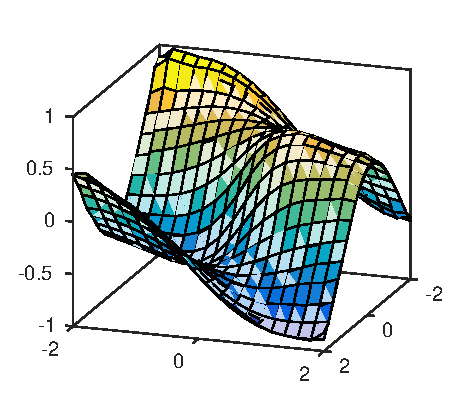
\includegraphics{plots/experiments/vdp/phi_hat.eps}
		%\caption{$\hat{W}_\varphi(t)$}
	\end{subfigure}
	\begin{subfigure}{0.5\textwidth}
		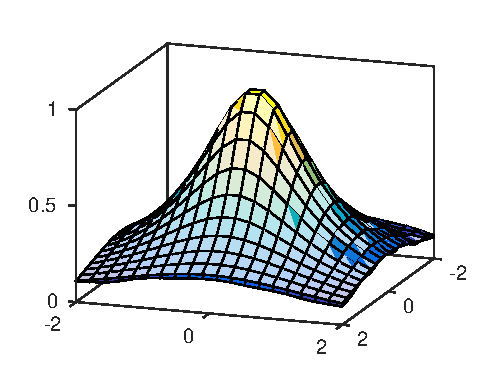
\includegraphics{plots/experiments/vdp/gamma_hat.eps}
		%\caption{$\hat{W}_\gamma(t)$)}
	\end{subfigure}
	\caption{Σύγκριση των συναρτήσεων $\varphi(x)$ (αριστερά) και $\gamma(x)$ (δεξιά) με τις προσεγγίσεις τους $\hat{\varphi}(x)$ και $\hat{\gamma}(x)$ αντίστοιχα για το πείραμα αναγνώρισης του ταλαντωτή \textit{Van Der Pol}. Με γκρι (transparent) απεικονίζονται οι πραγματικές συναρτήσεις ενώ οι χρωματισμένες επιφάνειες είναι οι προσεγγίσεις αυτών. }
	\label{fig:vdp_approximations}
\end{figure}

}

\subsubsection{Αποτελέσματα}
Χρησιμοποιώντας τις παραπάνω παραμέτρους, έγινε προσομοίωση του συστήματος κλειστού βρόγχου για $300$ περιόδους. Στο Σχήμα \ref{tab:vdp_schema_params} παρουσιάζεται η εξέλιξη κάποιων παραμέτρων των δυο νευρωνικών δικτύων. Από τα σχήματα αυτά φαίνεται πως ο χρόνος προσομοίωσης ήταν αρκετός για να σταθεροποιηθούν τα βάρη. Βλέπουμε επίσης, πως ενώ τα βάρη της $\hat{\varphi}(x)$ συγκλίνουν σε κάποιες τιμές χωρίς μεγάλες διακυμάνσεις, τα βάρη της $\hat{\gamma}(x)$ εκτελούν ταλάντωση - διαφορετικού πλάτους το κάθε ένα από αυτά - γύρω από κάποιες τιμές. Το φαινόμενο αυτό οφείλεται στην επιλογή μεγάλων κερδών $\beta_{\gamma_{ij}}$ και μπορεί να βελτιωθεί μειώνοντας τα αντίστοιχα κέρδη. Στην προκειμένη περίπτωση ωστόσο, για να αντιμετωπίσουμε το πρόβλημα αυτό, εξάγουμε τα βάρη $w_{\gamma i}$ ώς:
\begin{equation*}
	\bar{w}_{\gamma i} = mean_{t \in [t_a,t_b]} \{w_{\gamma i}(t)\}
\end{equation*}
όπου $[t_a,t_b]$ ένα επιλεγμένο χρονικό διάστημα στο οποίο τα βάρη κινούνται γύρω από μια σταθερή μέση τιμή. Στο συγκεκριμένο πείραμα χρησιμοποιείται ο μέσος όρος κατά τις δυο τελευταίες περιόδους της προσομοίωσης.

Σχετικά με την ποιότητα της προσέγγισης, στο Σχήμα \ref{fig:vdp_approximations} απεικονίζονται οι προσεγγίσεις των συναρτήσεων σε σύγκριση με τις πραγματικές, ενώ στα Σχήματα \ref{fig:vdp_phi_tilde} και \ref{fig:vdp_gamma_tilde} παρουσιάζουμε το σφάλματα $\tilde{\varphi}(x_1,x_2)$ και $\tilde{\gamma}(x_1,x_2)$ αντίστοιχα. Τέλος, στον Πίνακα \ref{tab:statistics_vdp} δίνουμε κάποια στατιστικά χαρακτηριστικά των προσεγγίσεων καθώς και της πραγματικής συνάρτησης έτσι ώστε να διευκολύνουμε την διαδικασία της αξιολόγησης αποτελεσμάτων.


\begin{table}
	\centering
	\begin{tabular}{  c | c | c | c | c | c }
		& $\min_{x \in \Omega_x}$ & $\max_{x \in \Omega_x}$ & Έυρος Τιμών & $\max(\abs{\tilde{e}})$ & Σχετικό Σφάλμα  \\ \hline \hline
		$\varphi(x)$ & $-0.8999$ & $0.8999$ & $1.7997$ & $0.1496$ & $8.31\%$ \\
		$\gamma(x)$  & $ 0.1111$ & $ 1.0$   & $0.8889$ & $0.0417$ & $4.69\%$
	\end{tabular}
	\caption{Στατιστικά στοιχειά προσεγγίσεων για τον ταλαντωτή \textit{Van Der Pol}}
	\label{tab:statistics_vdp}
	%\caption{Στατιστικά χαρακτηριστικά των προς αναγνώριση συναρτήσεων και του σφάλματος των εκτιμήσεων. (Για την συνάρτηση $f(x)g^{-1}(x)$ η μετρική \textit{NRMSE} δεν είναι ακριβής καθώς η μέση τιμή της συνάρτησης είναι ίση με το μηδέν)}
\end{table}

\begin{figure}
	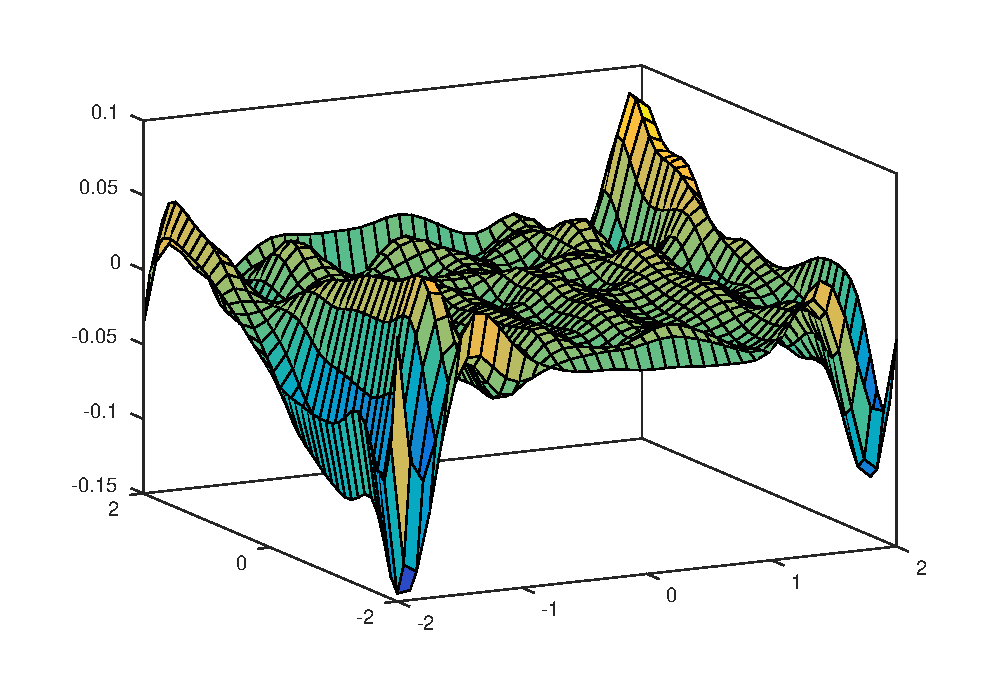
\includegraphics{plots/experiments/vdp/phi_hat_error.eps}
	\caption{Σφάλμα $\tilde{\varphi}(x)$ στο σύνολο $\Omega_x$}
	\label{fig:vdp_phi_tilde}
\end{figure}

\begin{figure}
	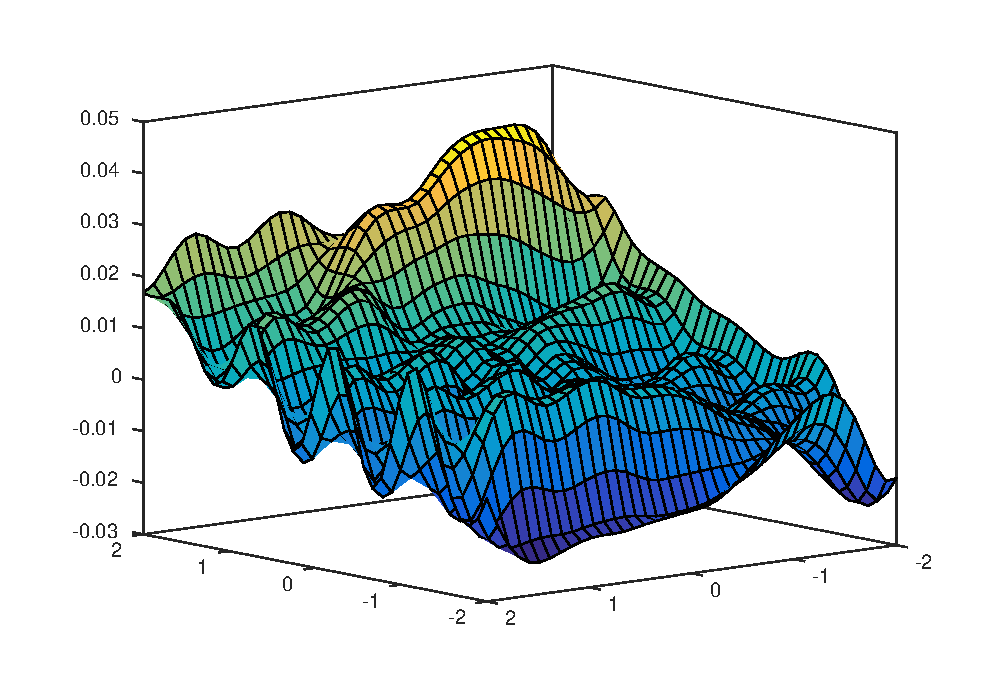
\includegraphics{plots/experiments/vdp/gamma_hat_error.eps}
	\caption{Σφάλμα $\tilde{\gamma}(x)$ στο σύνολο $\Omega_x$}
	\label{fig:vdp_gamma_tilde}
\end{figure}

Από τα παραπάνω στοιχεία οδηγούμαστε στο συμπέρασμα πως το σχήμα αναγνώρισης καταφέρνει να αναγνωρίσει επιτυχώς τις μη γραμμικότητες του  ταλαντωτή \textit{Van der Pol} παρόλο που δεν ανήκει στην κλάση συστημάτων \textit{Euler Lagrange} που μελετάμε. Κατά δεύτερον αξίζει να σημειωθεί πως μελετώντας τις γραφικές παραστάσεις \ref{fig:vdp_phi_tilde} και \ref{fig:vdp_gamma_tilde}, παρατηρούμε πως ενώ η ποιότητα των προσεγγίσεων είναι πολύ καλή στο εσωτερικό του $\Omega_x$, στο σύνορο φαίνεται πως η ποιότητα χειροτερεύει. Το αποτέλεσμα αυτό είναι αρκετά λογικό, αφού στο εσωτερικό του χώρου $\Omega_x$ υπάρχει επαρκής κάλυψη από γκαουσιανές ενώ αντίθετα τα σημεία που βρίσκονται στο σύνορο προσεγγίζονται από ένα λιγότερο πυκνό πλέγμα γκαουσιανών.


\subsection{Βραχίονας δυο βαθμών ελευθερίας}
Σε αυτό το τελευταίο πείραμα θα προσπαθήσουμε να αναγνωρίζουμε το δυναμικό σύστημα που περιγράφει την λειτουργία ενός βραχίονα δυο βαθμών ελευθερίας. Αρχικά παρουσιάζουμε τις εξισώσεις που περιγράφουν την λειτουργία του: 

\subsection{Ρομποτικός βραχίονας}
\label{exampleB}
Το τελευταίο σύστημα που θα εξετάσουμε είναι ο βραχίονας δύο βαθμών ελευθερίας, όπως παρουσιάστηκε στην εργασία\cite{bechlioulis2008robust}, ο οποίος περιγράφεται από την ακόλουθη δυναμική:
\[
M(q)\ddot q + C(q,\dot q)\dot q + g(q) = \tau,
\]
όπου $q = [q_1, q_2]$ είναι οι γωνιακές θέσεις [\si{\radian}], $\dot q$ οι γωνιακές ταχύτητες [\si{\radian/\second}], και $\ddot q$ οι γωνιακές επιταχύνσεις  [\si{\radian/\second^2}]. Ο θετικά ορισμένος πίνακας αδράνειας $M(q)$ ορίζεται ως:
\[
M(q) = \bmqty{M_{11} & M_{12}\\ M_{21} & M_{22}}
\]
με
\begin{align*}
M_{11} &= I_{Z_1} + I_{Z_2} + 0.25 m_1 \ell_1^2 
+ m_2(\ell_1^2 + 0.25 \ell_2^2 + \ell_1 \ell_2 c_2),\\
M_{12} &= M_{21} = I_{Z_2} + m_2 (0.25 \ell_2^2 + 0.5 \ell_1 \ell_2 c_2),\\
M_{22} &= I_{Z_2} + 0.25 m_2 \ell_2^2,
\end{align*}
όπου $I_{Z_1}$, $I_{Z_2}$ αναπαριστούν τις ροπές αδράνειας των συνδέσμων [\si{\kilo\gram \metre^2}], $\ell_1, \ell_2$ είναι τα μήκη τους [\si{\metre}], και $m_1$, $m_2$ οι μάζες τους [\si{\kilo\gram}]. Επιπλέον, χρησιμοποιείται ο παρακάτω συμβολισμός χάριν συντομίας:
\[\begin{array}{ll}
c_1 = \cos(q_1) & c_{12} = \cos(q_1 + q_2)\\
s_2 = \sin(q_2) & c_2 = \cos(q_2)
\end{array}\]
Ακόμη, ως $C(q, \dot q)$ συμβολίζουμε τον πίνακα που περιέχει τις δυνάμεις \textit{Coriolis}:
\[
C(q, \dot q)\dot q = \bmqty{-c \dot q_2 +  & -c(\dot q_1 + \dot q_2)\\ c \dot q_1 & 0}
\]
Με τον όρο $c$, συμβολίζουμε τον όρο $c = 0.5 m_2 \ell_1 \ell_2 s_2$ για συντομία. Επιπροσθέτως, $g(q)$ είναι το διάνυσμα των βαρυτικών ροπών:
\[
g(q) = 
\bmqty{0.5 m_1 g \ell_1 c_1 + m_2 g (\ell_1 c_1 + 0.5 \ell_2 c_{12}) \\
	0.5 m_2 g \ell_2 c_{12}}  
\]
όπου $g = 9.81 \si{\metre\per\second^2}$ είναι η βαρυτική σταθερά επιτάχυνσης. Τέλος, $\tau =[\tau_1, \tau_2]$ είναι οι ροπές [\si{\newton\metre}] οι οποίες δρουν ως είσοδοι ελέγχου. Οι ακριβείς τιμές των παραμέτρων του συστήματος αναγράφονται στον Πίνακα~\ref{tab:2dof_params}. 

Το σύστημα μπορεί εύκολα να έρθει στη μορφή~\eqref{eq:mimo_nonlinear} πολλαπλασιάζοντας από αριστερά με τον θετικά ορισμένο πίνακα $M^{-1}(q)$, καταλήγοντας στο ακόλουθο σύστημα διαφορικών εξισώσεων:
\[
\ddot q = - M^{-1}(q) \pqty{C(q,\dot q),\dot q + g(q)} + M^{-1}(q)u 
\]
Παρατηρώντας τις παραπάνω εξισώσεις εύκολα επαληθεύεται ότι το σύστημα ανήκει στην κλάση συστημάτων που μελετάμε αφού ο πίνακας $ M^{-1}(q)$ αφενός είναι θετικά ορισμένος, και αφετέρου είναι συνάρτηση μόνο των θέσεων $q_1$, $q_2$ και όχι των γωνιακών ταχυτήτων.

\begin{table}
	\centering
	\caption{Παράμετροι του συστήματος για το παράδειγμα~\ref{exampleB}}
	\label{tab:2dof_params}
	\begin{tabular}{l | ccc}
		\hline \hline
		$i$ & $m_i$ & $I_{Z_i}$ & $\ell_i$ \\ \hline \hline
		$1$ & $3.2$ & $0.96$ & $0.5$ \\\hline 
		$2$ & $2.0$ & $0.81$ & $0.4$ \\ \hline 
	\end{tabular}
\end{table}


{\begin{wraptable}{r}{0.3\textwidth}
		\centering
		\captionsetup{format=plain}
		\caption{Παράμετροι σχήματος αναγνώρισης για τον ρομποτικό βραχίονα}
		\label{tab:2dof_schema_params}
		\begin{tabular}{ l | r }
			\hline\hline
			\text{Parameter} & Value \\ \hline\hline
			$k$             & $30$   \\ \hline
			$\lambda$       & $1 $   \\ \hline
			$\beta_{\varphi} \;\text{(bias)}$     & $0.2$ \\ \hline
			$\beta_{\varphi} \;\text{(gaussian)}$ & $1$ \\ \hline
			$\beta_{\gamma} \;\text{(bias)}$     & $0.1$ \\ \hline
			$\beta_{\gamma} \;\text{(gaussian)}$ & $0.2$ \\ \hline
			$\rho_0      $ & $4$  \\ \hline
			$\rho_\infty $ & $0.02$  \\ \hline
			$l           $ & $2$  \\ \hline
			$\textit{ΔΤ} $  & $1$ 	\\ \hline \hline	
		\end{tabular}
	\end{wraptable}

\subsubsection{Σχήμα Αναγνώρισης}
Ορίζοντας το διάνυσμα καταστάσεων $x = \bmqty{q_1,\dot q_1,q_2,\dot q_2 }^T$, σκοπός της παρούσας εφαρμογής, είναι η αναγνώριση των άγνωστων συναρτήσεων
\begin{equation*}
	\Phi(x) = G^{-1}(x) f(x) = -\pqty{C(q,\dot q),\dot q + g(q)}
\end{equation*}
και 
\begin{equation*}
\Gamma(x_1, x_3) = G^{-1}(x_1, x_3) = M(q)
\end{equation*}
στο συμπαγές και κλειστό σύνολο $\Omega_x =\bmqty{-0.5,0.5}^4$. Για τον σκοπό αυτό θα χρησιμοποιήσουμε νευρωνικά δίκτυα RBF με τα  διανύσματα οπισθοδρομητών $Z_\varphi(x)$ για την αναγνώριση των συναρτήσεων του $\Phi(x)$ και $Z_\gamma(x)$ για τις συναρτήσεις του $\Gamma(x)$. Ομοίως με τα Παραδείγματα \ref{exp:wing_rock} και \ref{exp:vdp} τα κέντρα των οπισθοδρομητών επιλέγονται με τέτοιο τρόπο έτσι ώστε να καλύψουν ομοιόμορφα το σύνολο $\Omega_x$. Έτσι λοιπόν, τα κέντρα των οπιθοδρομητών $Z_\Phi(x)$ και $Z_\Gamma(x)$ τοποθετούνται στα πλέγματα
\begin{equation*}
\begin{matrix}
	\mathcal{C}_\Phi = \bigtimes\limits_{i=1}^{4}  \begin{Bmatrix}
	0 \pm  0.25 k, \quad  k = 1,2
	\end{Bmatrix}
&
\text{και}
&
\mathcal{C}_\Gamma = \bigtimes\limits_{i=1}^{2}  \begin{Bmatrix}
0 \pm  0.25 k, \quad  k = 1,2
\end{Bmatrix}
\end{matrix}
\end{equation*} 
αντίστοιχα. Στην συνέχεια επιλέγουμε τις διασπορές $\sigma$ έτσι ώστε δυο γειτονικές γκαουσιανές συναρτήσεις RBF να έχουν $75\%$ επικάλυψη, καταλήγοντας έτσι στην τιμή $\sigma = 0.2331$. Τέλος, σε κάθε προσέγγιση θα χρησιμοποιηθεί και ένας επιπλέον όρος πόλωσης (bias term). Οι υπόλοιποι παράμετροι του σχήματος αναγνώρισης παρουσιάζονται στον Πίνακα \ref{tab:2dof_schema_params}.

}

\begin{figure}
	\begin{subfigure}{0.5\textwidth}
		% This file was created by matlab2tikz.
%
\definecolor{mycolor1}{rgb}{0.00000,0.44700,0.74100}%
\definecolor{mycolor2}{rgb}{0.85000,0.32500,0.09800}%
\definecolor{mycolor3}{rgb}{0.92900,0.69400,0.12500}%
%
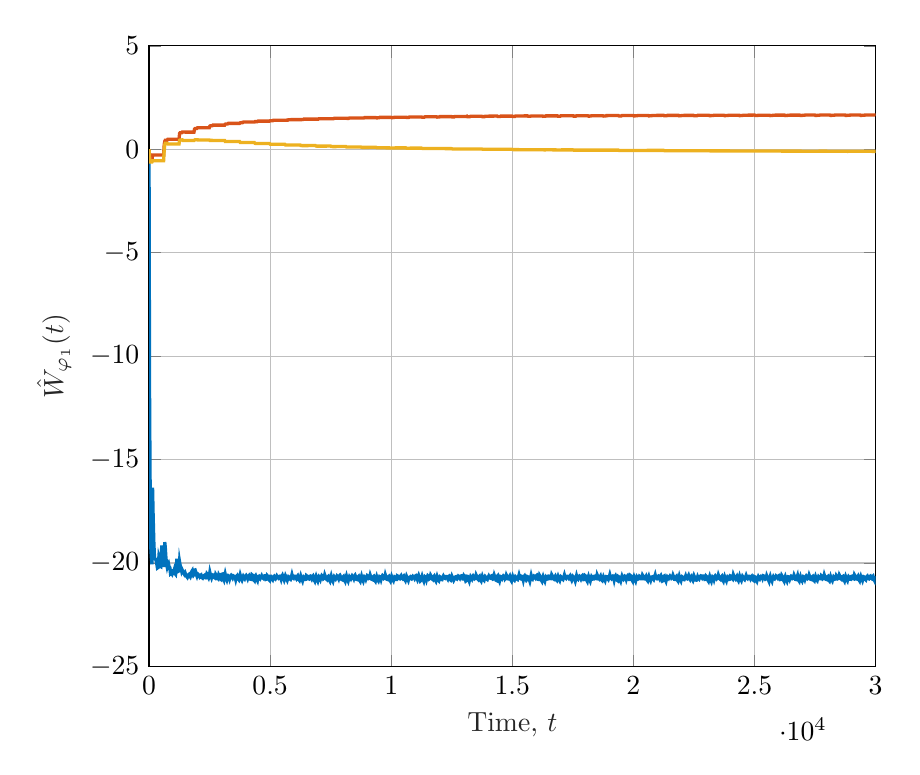
\begin{tikzpicture}

\begin{axis}[%
width=0.761\textwidth,
height=0.65\textwidth,
at={(0\textwidth,0\textwidth)},
scale only axis,
xmin=0,
xmax=30000,
xlabel style={font=\color{white!15!black}},
xlabel={Time, $t$},
ymin=-25,
ymax=5,
ylabel style={font=\color{white!15!black}},
ylabel={$\hat{W}_{\varphi_1} (t)$},
axis background/.style={fill=white},
xmajorgrids,
ymajorgrids
]
\addplot [color=mycolor1, line width=1.2pt, forget plot]
  table[row sep=crcr]{%
0	0\\
22.0010141601306	-11.6250756380832\\
40.006214029152	-15.1868213215675\\
58.4816655603645	-18.2310066142672\\
78.6879773681503	-19.3384505572103\\
100.575489070172	-19.7951175957132\\
123.3101701749	-20.0679332713953\\
146.228660635523	-16.3539808893911\\
172.199381604511	-17.7978798731201\\
199.216871204237	-18.9809402202627\\
226.142061781371	-19.7393703766866\\
253.772297893262	-19.8029810874032\\
282.213017586499	-19.8352434565895\\
312.89006128988	-19.9865503038491\\
347.705056364881	-20.2412509964488\\
380.612079327715	-20.2134744796167\\
405.795319896417	-19.7570380008583\\
430.056255439333	-19.8759526888171\\
458.369849905459	-20.1561375338897\\
488.768333195454	-20.1766186764326\\
513.0021832854	-19.4459834155314\\
533.191880132432	-19.1520956009044\\
554.687533079377	-19.4087430634172\\
578.451772799926	-19.9078156804571\\
603.376074201657	-20.1921009193211\\
628.00477153439	-19.8271275677471\\
649.79506491033	-18.9920706858247\\
671.834495370531	-19.2472445978819\\
696.193267098693	-19.7076777453913\\
720.364412559302	-20.0085208051787\\
749.284382873229	-20.1838666656113\\
776.20512120143	-20.069585962683\\
802.007542783762	-20.018796065382\\
831.034487188055	-20.1937623188933\\
861.011764461884	-20.229111205972\\
889.0061174537	-20.5255837098121\\
920.244393502478	-20.4966945479209\\
950.83492014186	-20.5430752320281\\
981.77304821838	-20.4253338457711\\
1011.22772520844	-20.4522919552619\\
1039	-20.3436249444494\\
1067.04456274024	-20.5006100581231\\
1097.98588926185	-20.546273315038\\
1126.78319450584	-20.3014945743635\\
1148.81605766601	-19.791506970203\\
1170.14953634024	-20.0940345173985\\
1192.34529951866	-20.2740462210713\\
1215.36345701218	-20.3969904696969\\
1239.8968705598	-20.3818163895412\\
1262.33614018248	-19.9499502013496\\
1282.68327601124	-20.0948266919004\\
1303.59919283675	-20.1762118361657\\
1352.02516904102	-20.4156484909581\\
1376.70631738191	-20.352613416595\\
1429.24933502657	-20.489135769476\\
1459.17708984501	-20.5462371747635\\
1490.00099732692	-20.4781299736569\\
1516.23387788289	-20.5636004240732\\
1550.66668012608	-20.6439725490018\\
1582.75625540383	-20.6936063195972\\
1616.81593034523	-20.5923933044942\\
1648.20604414454	-20.5574921415791\\
1676.02078559775	-20.6208344925581\\
1705.57737457926	-20.6709953978934\\
1736.39258040744	-20.5734656633358\\
1763.07560540824	-20.4156573906694\\
1785.71468998064	-20.373615911114\\
1808.05797066675	-20.5254252548766\\
1832.20716207739	-20.5948876209841\\
1857.12788227338	-20.5545620917692\\
1881.99763103162	-20.3489175392824\\
1903.76326242409	-20.3387222906058\\
1925.86568708504	-20.4226474145762\\
1949.69343372955	-20.554593696088\\
1975.51143158512	-20.6310032490219\\
2002.65543040722	-20.5227424329241\\
2029.54720384807	-20.5485251265709\\
2087.82811499125	-20.6659858386993\\
2119.21018741299	-20.6038331445525\\
2147.60974244864	-20.5812443752984\\
2179.22821710862	-20.7037765209243\\
2212.00087655821	-20.7312934301917\\
2248.27470887678	-20.627758147486\\
2275.31002342947	-20.607197063604\\
2304.04067707442	-20.7074745506434\\
2335.00461398508	-20.716520547805\\
2367.15670494568	-20.6404318790192\\
2392.07469832007	-20.5147877466115\\
2414.93507765002	-20.5434217674738\\
2438.21205209333	-20.6700549791058\\
2462.86399788344	-20.7246383711026\\
2489.54102798222	-20.6327054030226\\
2512.87867535083	-20.4543878733748\\
2535.76902775786	-20.5652452821378\\
2559.03789619781	-20.632060144093\\
2583.08717427489	-20.7136625815074\\
2610.55031994384	-20.613008429922\\
2636.31609578053	-20.5857764879111\\
2663.7054471777	-20.6189305100597\\
2692.54660604851	-20.7017823287642\\
2725	-20.7271236636261\\
2753.26802134881	-20.5533035606131\\
2783.80568827383	-20.6126203670174\\
2814.76898850397	-20.7207808229032\\
2849.73400486278	-20.7596048083215\\
2880.88097628015	-20.5761715987755\\
2909.70441151558	-20.6368093228884\\
2939.34543624319	-20.7459648152035\\
2970.07801066419	-20.7812192602323\\
3001.88819517193	-20.5488556235978\\
3025.18012683544	-20.5397020767523\\
3049.88755532052	-20.6944592120599\\
3096.00359725381	-20.8214498436027\\
3146.00685317941	-20.5420902199839\\
3168.56515246117	-20.6557524220079\\
3217.22937795712	-20.8135034120751\\
3244.95249248798	-20.6977511910154\\
3273.0046193674	-20.6282797406238\\
3300.94222580976	-20.6575568584594\\
3329.29257993141	-20.7696903150281\\
3360.82950483446	-20.6459991476295\\
3392.16392443045	-20.597915460392\\
3425.37713991607	-20.6485373536561\\
3456.05888044651	-20.7209652537276\\
3489.02087292794	-20.6296264082448\\
3551.62247646616	-20.6745098551837\\
3579.34357965102	-20.7992704971184\\
3610.37836927607	-20.6432116307988\\
3640.53774637625	-20.605924048341\\
3666.50400010544	-20.6869592865987\\
3690.46373933997	-20.7741083258443\\
3714.44523585703	-20.8119970370826\\
3740.21303904782	-20.7196166550493\\
3765.57874719471	-20.5835800805471\\
3789.5000012821	-20.6781658709879\\
3813.41854503588	-20.7536809490739\\
3838.02589677472	-20.8175224902006\\
3865.14487520794	-20.7179792021525\\
3893.08800109858	-20.6407387090367\\
3950.32685173723	-20.7505906155857\\
3980.91924208061	-20.6479978010138\\
4010.93781687778	-20.603797352418\\
4041.00742618711	-20.6638602379426\\
4074.62788696224	-20.7611226323861\\
4104.76099217656	-20.6616888144854\\
4135.52411753067	-20.6115555823344\\
4164.84363872227	-20.6797076072908\\
4191.67724116229	-20.7845018505213\\
4220.34181600386	-20.7917795530375\\
4251.88666221631	-20.5722708759713\\
4277.8975024907	-20.5982788278234\\
4302.65307642276	-20.7384174866202\\
4326.35727686555	-20.8169812341985\\
4351.12609962662	-20.8509397279086\\
4378.45967308257	-20.64039597191\\
4402.99755749093	-20.6039439998822\\
4427.18088671436	-20.6737883919523\\
4450.88992534439	-20.7921771923029\\
4475.64313726746	-20.8504420708232\\
4502.89300107902	-20.6661341916697\\
4532.11608990744	-20.6463551005181\\
4559.46164014736	-20.7183539744146\\
4588.83383393395	-20.7613104506127\\
4648.901018774	-20.6229095445742\\
4679.10286946986	-20.7080899854773\\
4708.28132625591	-20.73385750546\\
4737.59335486815	-20.6282719749433\\
4767.63086443802	-20.6239387636888\\
4822.81141342114	-20.7944597622081\\
4850.46800446488	-20.7827576756717\\
4878.99670483398	-20.6076634825622\\
4903.78169939709	-20.6382891097674\\
4928.73021140362	-20.7625383791892\\
4952.19546971423	-20.8119157908477\\
4976.5756600961	-20.8411845019691\\
5003.27888956456	-20.6405020493075\\
5028.55203787279	-20.6396362447631\\
5053.02400866113	-20.7156369455806\\
5076.86278048775	-20.7751425544702\\
5101.9766380536	-20.8111531948198\\
5129.07743266448	-20.6971333025504\\
5157.80285819941	-20.6622160904808\\
5185.91979487858	-20.7475306173837\\
5215.10248702628	-20.7756534988366\\
5275.28244402961	-20.6248580792853\\
5305.04877713639	-20.6838663732306\\
5335.23733968329	-20.7201749147171\\
5365.21927850344	-20.6562321397432\\
5395.93401645824	-20.6433751384684\\
5426.34678531726	-20.700568367607\\
5453.32913367534	-20.7904275532128\\
5481.1166906102	-20.662924130731\\
5510.08629175029	-20.5983998902666\\
5583.74501536359	-20.8290929051655\\
5609.83735346909	-20.7443050438815\\
5635.53931474248	-20.62938000336\\
5660	-20.694553972633\\
5684.00326531268	-20.7743972623575\\
5707.49671665597	-20.8331723217925\\
5733.79545157124	-20.7293150490732\\
5760.09513935152	-20.6593767074737\\
5787.50469944528	-20.6804280018659\\
5815.92577524783	-20.7727127916041\\
5844.51149746819	-20.7959975334998\\
5872.90032774283	-20.7076993876144\\
5902.03078964411	-20.5709112056866\\
5932.854312785	-20.7118737786368\\
5963.41988993171	-20.7381880526846\\
5995.06924468521	-20.6399636528986\\
6023.71360667713	-20.6447281687069\\
6053.12309724616	-20.7076612081801\\
6081.14536412859	-20.7552149513212\\
6110.75890227409	-20.6617313590359\\
6139.02088856078	-20.6217474578625\\
6190.23479392473	-20.8041838127028\\
6214.02582533636	-20.8414816244294\\
6240.42431496458	-20.7483682583443\\
6265.81609611158	-20.6363188026407\\
6289.57167888949	-20.7237518596849\\
6337.00612441976	-20.860037359831\\
6362.00058271465	-20.7344759342886\\
6387.84319157732	-20.6666661199379\\
6416.69670851818	-20.6912927000085\\
6445.91815529961	-20.7963980155073\\
6474.89482951662	-20.7914166412011\\
6502.13086356609	-20.6132495205711\\
6531.38454646943	-20.6411039860286\\
6563.00087664022	-20.73151451995\\
6595.2580995895	-20.7563775717499\\
6625.41561612354	-20.6499280421231\\
6653.52465348812	-20.6371988266474\\
6681.66633450691	-20.7215291289394\\
6709.16773213907	-20.7719709045887\\
6738.24895692791	-20.666338301733\\
6767.41654065242	-20.6302806694184\\
6794.67839846663	-20.7428853880701\\
6819.11592911143	-20.8212577004342\\
6843	-20.8725847089408\\
6870	-20.7292654997946\\
6895.64554063634	-20.6444589340317\\
6943.2747252336	-20.8151307490516\\
6967	-20.8752407829161\\
6991.90976691926	-20.7577900588658\\
7019.85454724813	-20.6602595941113\\
7049.88892602786	-20.7000470390594\\
7078.03034703268	-20.7837635933429\\
7105.0450997172	-20.6726434294724\\
7133.08220720066	-20.6094939682152\\
7165.20628767484	-20.6535131455494\\
7198.96597779813	-20.7589005988521\\
7227.8895480703	-20.7283025769138\\
7256.13586903482	-20.5775570389487\\
7315.32566513611	-20.7684531056984\\
7343.51664217019	-20.8001171976284\\
7372.81082181324	-20.6792331117504\\
7399.30890412766	-20.6520357884292\\
7425.90517858284	-20.7688602746675\\
7449.1860656328	-20.8358336440324\\
7471.24521644833	-20.8804459329513\\
7499.39294272152	-20.742173054321\\
7523.04429107055	-20.6389116693681\\
7547.18978972044	-20.7520472209508\\
7595.64356987678	-20.8788633401091\\
7620.16911782198	-20.7597658722698\\
7648.63306268269	-20.6632124472417\\
7678.28292029199	-20.708196396823\\
7706.92941380541	-20.7632988757323\\
7762.06455622318	-20.6302455161567\\
7796.11639457328	-20.6764541337361\\
7827.85215716439	-20.7580003675102\\
7855.54781153105	-20.6311413261901\\
7884.49050533435	-20.5985513656451\\
7915.04603274785	-20.6792529568629\\
7944.97459151303	-20.7881509144609\\
7970.95249232475	-20.803914821623\\
8000.20051690676	-20.6805150435575\\
8025.24128760182	-20.6536310995652\\
8050.71981864595	-20.7836827840401\\
8096.86391217875	-20.8858041419007\\
8125	-20.7312773093763\\
8150.27806551976	-20.6345466705206\\
8173.37481975988	-20.7399865621665\\
8197.71056301703	-20.8206557602462\\
8220.70994001865	-20.8770573632937\\
8245.54108682131	-20.7577545642198\\
8273.75847969247	-20.6654857003196\\
8331.00326681594	-20.7650775525763\\
8358.30361291683	-20.684470472901\\
8386.03109157838	-20.622664124865\\
8420.73851300205	-20.6793356990165\\
8452.9694793095	-20.7581224214009\\
8480.00533694809	-20.6427531945337\\
8509.1960041915	-20.5950882374345\\
8538.13866858349	-20.6811810042382\\
8568.57877024686	-20.7931428713673\\
8596.01359391017	-20.8022244156818\\
8625.2225427878	-20.6783773725183\\
8650.33557885922	-20.6511671817971\\
8674.80655530921	-20.770492441512\\
8697.67237086323	-20.8387727270565\\
8720.90601312488	-20.8821625457458\\
8748.51919023621	-20.7392255274062\\
8772.87097714111	-20.6445814007675\\
8795.86607076198	-20.7494304028369\\
8844.4928187413	-20.8735573873673\\
8869.33593743871	-20.7598870654583\\
8895.9912597712	-20.669559457001\\
8926	-20.6996730370884\\
8953.20734732295	-20.7828145767817\\
8979.93459639306	-20.6890698795214\\
9007.81729726913	-20.6144836194544\\
9040.045282482	-20.6489025120645\\
9075.52207723869	-20.7475187327836\\
9104.1511688793	-20.7330556408961\\
9132.86143558719	-20.5868930366487\\
9192.43610570643	-20.785325953897\\
9220.53578756602	-20.8003265016923\\
9249.90714044826	-20.6807201501942\\
9274.47252934429	-20.6560630200765\\
9298.8868417866	-20.7672193759681\\
9322.38171134601	-20.8430020565102\\
9345.85712704332	-20.8803424541002\\
9372.86747478923	-20.7382616822761\\
9397.15597424958	-20.6561371117859\\
9420.72352081034	-20.7487891111014\\
9445.50375354124	-20.8206455137624\\
9470.03276370854	-20.8646863260801\\
9494.72001503564	-20.7621727040678\\
9520.95048670254	-20.6699179553871\\
9551.22622921719	-20.6961351337632\\
9578.49052189168	-20.793879691857\\
9606.00653581649	-20.6698070061248\\
9634.2861894239	-20.6188314325045\\
9665.6974778227	-20.6701834608029\\
9700.10300010465	-20.7488236370191\\
9728.40748189801	-20.7276240175634\\
9757	-20.5712565206668\\
9816.70054209479	-20.7855826979539\\
9845.15192750833	-20.7969097815221\\
9873.8479973309	-20.6763701794443\\
9897.90219557842	-20.6535347895078\\
9920.89884936298	-20.7602613450144\\
9945.12089641397	-20.8272047748796\\
9967.75420076866	-20.8713183503933\\
9991.49619615414	-20.7568736185312\\
10015.6381273123	-20.6587163676013\\
10040.4748984579	-20.7421760727993\\
10065.1471262701	-20.8068872249605\\
10088.7271597519	-20.8538892168217\\
10112.4336380042	-20.7403868901456\\
10137.0002924905	-20.6744507770381\\
10166.1718921816	-20.6993872363673\\
10195.8567315288	-20.7988285522333\\
10223.5760787423	-20.7984309274434\\
10251.721081843	-20.6213561599216\\
10281.0559083679	-20.6410252168098\\
10312.9771602807	-20.733014041125\\
10345.3478862884	-20.754231744384\\
10375.3874619665	-20.6522824130734\\
10402.6362120879	-20.6144325022942\\
10431.8095810998	-20.7236342575088\\
10460.2986991755	-20.752881447821\\
10487.7856608359	-20.664414365503\\
10514.7886434181	-20.6330861719507\\
10563.1712794126	-20.8000047521455\\
10586.0005841636	-20.8471996846456\\
10633.2591140727	-20.6428892969343\\
10706.7608688401	-20.8401667372564\\
10729.9650921833	-20.7384164053401\\
10754.0603000727	-20.7001313667351\\
10782.9061608417	-20.6746018559606\\
10811.2851009249	-20.7561493346511\\
10838.8122545639	-20.7723676319438\\
10897.4814330221	-20.6460680751625\\
10928.3126833084	-20.6796059587869\\
10958.711617081	-20.7410420601227\\
10987.9799728329	-20.6354130723412\\
11017.4923231744	-20.616069319145\\
11047.7705521524	-20.7137675519225\\
11078.2020763132	-20.7952721845249\\
11105.0168981176	-20.6766052651365\\
11132.0065355145	-20.6015238218388\\
11180.837268897	-20.7701650560703\\
11204.007544266	-20.8691773690989\\
11226.8567328421	-20.8447498514433\\
11275.9122181789	-20.6512647154486\\
11299.2301155132	-20.7440525871534\\
11346.3113295137	-20.8760687996473\\
11369.9070264847	-20.75587315343\\
11396.1920568177	-20.6677404792645\\
11426.2572232203	-20.6976518632473\\
11453.8759103667	-20.8050851878761\\
11480.0011726298	-20.6834164593747\\
11507.3670018857	-20.6146649516668\\
11538.720233748	-20.6509666440288\\
11570.9466442886	-20.7718729820663\\
11600.6634840819	-20.7468632523523\\
11629.2552327251	-20.5947637748905\\
11659.0032659006	-20.6548945546019\\
11689.6948229364	-20.7688579945498\\
11718.3809448164	-20.7989113522563\\
11746.5537039263	-20.6807339818952\\
11771.215167891	-20.6446776468438\\
11796	-20.7605250875567\\
11820.3638618617	-20.8239824067823\\
11844.2096572353	-20.872020260289\\
11867.0997540751	-20.7577653012668\\
11891.9613852194	-20.658962472713\\
11916.4034631606	-20.7489250715262\\
11940.983824851	-20.8221223594919\\
11964.2687183622	-20.8536712461937\\
11987.6605741644	-20.738223770164\\
12012.5155860812	-20.6699206574085\\
12041.5983106503	-20.6948699255481\\
12070.8657044134	-20.7996717673814\\
12096.9154233274	-20.8069664310133\\
12125.438981148	-20.7126458957282\\
12154.4890639786	-20.6398548233046\\
12185.1733878168	-20.7154414888464\\
12215.0009897092	-20.73558181318\\
12246.0127866337	-20.6544755165633\\
12275.6869599745	-20.6574687762586\\
12333.4796243527	-20.7714234103587\\
12360.1718877862	-20.6634252638105\\
12387.0208345802	-20.6399732190148\\
12436.6726366018	-20.8067123183719\\
12459.9695211232	-20.8294324263115\\
12483.4328512503	-20.7599774735099\\
12508.4831068864	-20.6473802300679\\
12534.136852221	-20.7160226789492\\
12556.6862208933	-20.7637472100469\\
12580.8165474457	-20.834014449636\\
12604.5628662644	-20.7790670760405\\
12628.5285925226	-20.6906965174458\\
12658.1267128354	-20.6746308755464\\
12685.9559345771	-20.760504468115\\
12713.2828198036	-20.7778615273783\\
12770.5986287998	-20.6432803064745\\
12802.8282503582	-20.683829227175\\
12831.4493927615	-20.733863302321\\
12860.9340644743	-20.6378862196252\\
12891.0928447515	-20.6276217394952\\
12921.255739756	-20.7092286615807\\
12951.5574989548	-20.770521027549\\
12978.4998523276	-20.7689984515564\\
13005.6533107439	-20.6248713191417\\
13030.331662239	-20.6659333109965\\
13078.9713339615	-20.8695780777198\\
13102.3774084584	-20.8444664109702\\
13126.80134148	-20.6430088051711\\
13151.266115007	-20.6487019136075\\
13174.9019137353	-20.7458625284416\\
13221.9456253719	-20.8819571629028\\
13245.9125869108	-20.7581248918541\\
13275.2974756981	-20.6618739239348\\
13330.7232666123	-20.7700943523705\\
13356.5705521864	-20.669181301706\\
13383.9712257909	-20.6209052778977\\
13415.677459534	-20.6702315566072\\
13448.1312588489	-20.7584602906572\\
13477.7680655411	-20.7303440304313\\
13506.0426017832	-20.5839671644135\\
13534.0065310949	-20.6546547474609\\
13562.4580067404	-20.7600271174488\\
13590.7969318192	-20.7936795851383\\
13620.0278190022	-20.6650771339628\\
13644.9935447296	-20.6392856807543\\
13669.6292157111	-20.7498389598404\\
13693.5466780383	-20.8270648313264\\
13715.8071302804	-20.8691308448942\\
13764.1705494564	-20.6547263872344\\
13811.6959168231	-20.8098848081681\\
13834.489442061	-20.8389257162344\\
13857.4897628536	-20.7383284026873\\
13882.7349200257	-20.6581622904268\\
13911.7406837453	-20.6955935132173\\
13940.7620066004	-20.7765902107967\\
13967.7383360001	-20.7994651775844\\
13995.1684381262	-20.7086954340448\\
14025.2338670158	-20.638245040107\\
14055.7406594169	-20.7182030866534\\
14084.884685574	-20.7305463394478\\
14114.5912768317	-20.6394218563873\\
14143.4384205957	-20.6231666734166\\
14172.8056370825	-20.7129046219488\\
14201.415634691	-20.7803322788568\\
14228.5361710052	-20.768126180832\\
14256.5731685873	-20.6020144439899\\
14306.9133754123	-20.7694016731875\\
14329.5663184	-20.8375974074515\\
14353.2580536511	-20.8503117650835\\
14377.1570571788	-20.6436929769989\\
14401.8209138554	-20.6139768050562\\
14425.1169722494	-20.7445238863766\\
14471.2388082612	-20.8760159336998\\
14495.4914969554	-20.7523858173299\\
14525.1420207213	-20.6620202387967\\
14551.9577947941	-20.6774778688668\\
14580.2024648846	-20.7420649113301\\
14605.9629734741	-20.6725269713243\\
14633.6273769202	-20.6221525307337\\
14664.85934408	-20.652371600976\\
14696.5063819466	-20.7654184061867\\
14726.9783652478	-20.7127058893166\\
14755.2192682638	-20.5836335099266\\
14783.3056386544	-20.6516823572892\\
14810.9548953555	-20.7643625026685\\
14839.4735995488	-20.7699220560389\\
14868.5099101597	-20.6917094544697\\
14894.3433408788	-20.6392551722456\\
14919.6326456098	-20.7499976321487\\
14943.1590111958	-20.8262749369314\\
14965.7274326144	-20.869864492015\\
14989.3641727455	-20.7422527660419\\
15014.3294044259	-20.6542525174591\\
15038.0772052373	-20.7383829808387\\
15062.1776645775	-20.8089298036066\\
15085.3632902977	-20.8337258909087\\
15108.7433912122	-20.7441425559882\\
15133.0316545838	-20.6625700535806\\
15161.8009549125	-20.6956470252589\\
15191	-20.7807267376629\\
15219.0092411525	-20.8010641171932\\
15246.7735819563	-20.706894606792\\
15277.1352852273	-20.5817221818652\\
15307.6677756988	-20.7128647598111\\
15337.2443107477	-20.7415631422264\\
15370.0104251555	-20.6386557305123\\
15397.194967148	-20.6513138069931\\
15427.1826020863	-20.6800771527087\\
15454.0704976149	-20.8141662512171\\
15481.395200234	-20.6616888165372\\
15509.2076279008	-20.6213039847025\\
15534.1167957046	-20.6934369984156\\
15558.7139915151	-20.7835325071319\\
15581.1003785149	-20.8330040242981\\
15604.5834425486	-20.7995330152189\\
15628.8448444191	-20.6650821528419\\
15653.9347506205	-20.6796699731167\\
15677.0615609375	-20.7108535931293\\
15724.6825486649	-20.8797197678687\\
15777.020646434	-20.6072524739466\\
15804.5298903839	-20.7359433740748\\
15832.8325134945	-20.7713170030802\\
15860.0109582337	-20.6690018113986\\
15888.1557755691	-20.6342800472303\\
15952.0345566075	-20.7262363327609\\
15981.538122626	-20.6287028084262\\
16010.8065594949	-20.6003654154629\\
16070.2172722494	-20.7928732730397\\
16098.0277957288	-20.7947853800542\\
16126.785020362	-20.6000803365969\\
16151.4728139407	-20.6474353046542\\
16176.3429851375	-20.7686988450769\\
16198.3689235713	-20.8343928303475\\
16221.3721908456	-20.8782816776402\\
16245.945218859	-20.7416092260173\\
16270.5953929757	-20.657906004235\\
16294.2798193255	-20.7439863931759\\
16318.0725116342	-20.8189728987527\\
16340.67096354	-20.8760123419634\\
16364.0021891982	-20.7434272782666\\
16390.1470973242	-20.6721680439587\\
16420.8023746857	-20.7161488141901\\
16451.0556118142	-20.7763629305773\\
16477.5973141391	-20.7696497510806\\
16504.9108336506	-20.6363173886857\\
16534.5212148143	-20.6392761662646\\
16565.5304922078	-20.7517826925905\\
16598.8016180805	-20.7573902992226\\
16628.1967593287	-20.5727814593265\\
16657.1931626649	-20.6365999840818\\
16685.2023858603	-20.7362729663146\\
16712.6763810837	-20.7676044932668\\
16741.8931368275	-20.6876340732779\\
16768.8612150588	-20.6434055741702\\
16793.4788901552	-20.7515748844016\\
16816.0534819271	-20.8209121034051\\
16838.9793480109	-20.8456198472013\\
16862.9833444179	-20.7437340073593\\
16887.5265756772	-20.6584356282619\\
16911.0036784575	-20.7380188175193\\
16957.9615132919	-20.8415258792011\\
16980.9287698765	-20.7385258832546\\
17005.8539722484	-20.6613861551341\\
17035.8495352092	-20.6930123651691\\
17065.781146127	-20.7765863395252\\
17093.0068573718	-20.8016047974343\\
17121.754533053	-20.7063613611972\\
17152.2018283804	-20.5842760039486\\
17182.0594295384	-20.7077662799893\\
17213.1815621645	-20.7402508803607\\
17245.446276493	-20.6480742998574\\
17274.7984762561	-20.6445728345134\\
17303.1286475359	-20.7076574644889\\
17330.2756150421	-20.7437740657551\\
17358.2693719431	-20.6778496660045\\
17386.3975610482	-20.6285519641788\\
17411.0069076296	-20.7111536148113\\
17457.108789933	-20.8359245518041\\
17480.0842295621	-20.7703188344203\\
17505.0828694087	-20.6532703563535\\
17552.0134652983	-20.7102664215781\\
17600.0023503888	-20.8719277456003\\
17652.4554845402	-20.6199730579101\\
17680.8323722937	-20.7370663168731\\
17708.150632174	-20.7720982395731\\
17735.3185641035	-20.6630438164502\\
17763.56400634	-20.6347524590819\\
17797.016465427	-20.6845028865318\\
17827.8144537821	-20.7588332173545\\
17858	-20.6463632292616\\
17887.4075925319	-20.6138516533283\\
17917.0090322203	-20.6913103996703\\
17946.0062103847	-20.803421389508\\
17974.1691589159	-20.7995839561991\\
18002.7254676898	-20.6101443727748\\
18027.8101805291	-20.6340164437352\\
18074.2747532657	-20.836853245095\\
18096.9958707284	-20.8849275963294\\
18122.2102461317	-20.7418689695223\\
18145.9882358695	-20.6561081883156\\
18169.113120784	-20.7461841837758\\
18192.6440738411	-20.8169522593998\\
18216.0415658966	-20.8750380529491\\
18240.0021974845	-20.7464384652558\\
18266.384353786	-20.6636247981587\\
18325.0311694252	-20.7790776449801\\
18351.1122495609	-20.7758491453424\\
18378.8699457833	-20.6460680061609\\
18410.1274116481	-20.6361998264147\\
18441.1020676679	-20.7529274157896\\
18473.8987137187	-20.7583031278373\\
18503	-20.5741514525907\\
18530.9690073923	-20.6517648434237\\
18559.0378855896	-20.7422899306293\\
18586	-20.7733029987758\\
18615.5714323204	-20.6924737969421\\
18642.8464521891	-20.6360106430111\\
18668.0135147367	-20.7475924159808\\
18690.6646509274	-20.821840954457\\
18713.0048108393	-20.8476535326627\\
18737.0110628941	-20.7515442205004\\
18762	-20.6692449820657\\
18785.6569282122	-20.7359654513821\\
18808.3481800664	-20.7803730508531\\
18832.7609698958	-20.843498381113\\
18856	-20.7397793245364\\
18881.2388762852	-20.6608534139887\\
18910.3390336443	-20.6678216253749\\
18940	-20.7574208887672\\
18965.828677836	-20.797958134568\\
18995.8182342013	-20.7053092887181\\
19026.8933326186	-20.573985722971\\
19057.1404065991	-20.7067265548794\\
19087.000877914	-20.7453891251462\\
19120.1451684005	-20.6556910596701\\
19148.3710327109	-20.6354666606021\\
19177.2432220979	-20.6824383719904\\
19203.9233202104	-20.8160479855978\\
19231.6143828844	-20.6608292869096\\
19260.2175000999	-20.6150867786346\\
19285.024269758	-20.6906405482114\\
19308.7938219681	-20.7833614364063\\
19331.1211128609	-20.8335473824191\\
19354.2975650169	-20.8542744996957\\
19379.7347567497	-20.6571943264062\\
19404.7134473162	-20.676811108533\\
19427.1733183914	-20.7167067347109\\
19451.1555803121	-20.8129025242961\\
19474.8768779387	-20.8756084810557\\
19499.0321768979	-20.7562198284104\\
19527.8932173981	-20.642332828389\\
19556.8778384953	-20.7335700125041\\
19583.7140697174	-20.7733740917465\\
19611.52170378	-20.68338728862\\
19641.5831695434	-20.6342454119767\\
19675.5244845488	-20.6652921247769\\
19704.3547978078	-20.7782629467147\\
19734.1929729785	-20.6551110946129\\
19764.4646903608	-20.6148558336645\\
19823	-20.7937406735655\\
19850.1674720539	-20.7917285528893\\
19878.2830113884	-20.6083073777008\\
19903.1948038953	-20.6315775137118\\
19927.6261840254	-20.7628988239485\\
19949.7780582885	-20.839044867691\\
19972.261740706	-20.8839316322046\\
19997.9334846695	-20.7402740421167\\
20021.9134510645	-20.6657477173831\\
20067.492799671	-20.817275218109\\
20090.7017011282	-20.8751730622571\\
20114.7423141378	-20.7593181536358\\
20140.8222802608	-20.6681129552053\\
20201.2605662048	-20.7726374285885\\
20227.2832062315	-20.7596217586761\\
20255.6997318595	-20.6397028406682\\
20286.8548914897	-20.6638252653211\\
20319.2584301617	-20.7603678675077\\
20349.7580938724	-20.7616506597915\\
20379.191284371	-20.5943283175111\\
20407.8971142185	-20.6492767374984\\
20436.5504507483	-20.7657846938455\\
20464.159705265	-20.7680683574326\\
20493.6825172191	-20.6885330326804\\
20519.8580519221	-20.6417031433957\\
20544.346668614	-20.7478706783077\\
20566.7333416876	-20.8227109317777\\
20589.6154201919	-20.8587648587018\\
20613.8004751335	-20.7434172058493\\
20639.002184571	-20.6575948707978\\
20662.2431619448	-20.7472308668475\\
20684.563545512	-20.7826380792139\\
20708	-20.8421134737109\\
20730.980467321	-20.7406434961631\\
20755.6801579311	-20.6795535908714\\
20785.2384644385	-20.6686721190199\\
20815.3598074557	-20.7583652880567\\
20840.8595656164	-20.7992175122999\\
20870.7253095709	-20.7054793575262\\
20902.1612640542	-20.5832830799591\\
20931.3264340366	-20.7127563702488\\
20961.2297979928	-20.7424216402687\\
20994.0182029041	-20.6556028584819\\
21023.1906600477	-20.6376098594992\\
21052.7071308584	-20.7109314249101\\
21079.9056418274	-20.7659185984994\\
21107.0097902397	-20.6662551796835\\
21135.2546177424	-20.6141489095025\\
21182.411577734	-20.7693101679761\\
21204.3643753374	-20.8692007537575\\
21227.8168186376	-20.8533526053943\\
21253.0273905046	-20.6494330215246\\
21277.4258184752	-20.630361053536\\
21300.8074865441	-20.754936866455\\
21346.1690303694	-20.8769514806881\\
21370.1651190634	-20.7573021111348\\
21398.9066495408	-20.6681988957753\\
21455.1205657992	-20.7451943180895\\
21481.8252842627	-20.6754101042607\\
21510.6977755172	-20.6269751132932\\
21544.7947207753	-20.6759604764993\\
21575.4123758837	-20.7446939547517\\
21604.444208453	-20.718382911753\\
21635.1577173304	-20.5943033609983\\
21664.8867823646	-20.6827312687165\\
21693.3310105	-20.7919815998575\\
21720.463179188	-20.7933840682635\\
21750.1153650781	-20.6847908083437\\
21774.8078555814	-20.6543495807891\\
21798.6747108913	-20.7670704975462\\
21820.5429186501	-20.8367240242769\\
21843.1746643419	-20.8755293260074\\
21867.9277910391	-20.7563304265495\\
21892.4352381078	-20.64987674847\\
21916.6338079603	-20.7534374308671\\
21961.4078319811	-20.8581422164025\\
21985.4633600679	-20.7283073936196\\
22010.5877227452	-20.6652397028301\\
22040.4255038917	-20.6891268867403\\
22070.8935941705	-20.7999126058894\\
22097.0199964571	-20.8080447162247\\
22156.7543914165	-20.6309669656657\\
22185.8441492491	-20.7393768954098\\
22216.8052825797	-20.7595350699303\\
22278.2241326767	-20.6106076300966\\
22306.812491607	-20.7253197379432\\
22334.0260371876	-20.7786785157405\\
22361.3289898076	-20.6677338143963\\
22389.8083203582	-20.6376305745544\\
22436.2630625386	-20.7969132426952\\
22458.5658484209	-20.8435185720737\\
22482.2685834444	-20.7573948945756\\
22507.11702482	-20.6334226437175\\
22578.4741394584	-20.826069158782\\
22601.9070106313	-20.8303862737739\\
22625.6827884191	-20.7808351764579\\
22654.7638888237	-20.6670442342547\\
22684.4076349532	-20.7426550773998\\
22710.7677477311	-20.7763623901992\\
22739.4570755265	-20.6820854061625\\
22770.8230271961	-20.6391372449798\\
22801.0158882327	-20.6696905841709\\
22830.1695816702	-20.7165386161942\\
22860.2114887462	-20.6274176938641\\
22890.8544211917	-20.6286311418116\\
22949.2559566176	-20.794915281087\\
22975.8026610568	-20.7882394652806\\
23004.2401238047	-20.6344328095438\\
23029.0037727216	-20.6636961901022\\
23074.9659016501	-20.8392038444144\\
23097.5967481729	-20.8803483109223\\
23122.991354983	-20.7409453450673\\
23147.6895397034	-20.6541171179924\\
23171.3632244564	-20.7518583719138\\
23218.4158634391	-20.8795484721413\\
23241.6229597534	-20.7602134602021\\
23270.6833116223	-20.6664889445274\\
23301.4107889625	-20.6949604164511\\
23328.6613768868	-20.7967383562464\\
23355.675568748	-20.675070299254\\
23384.6414632861	-20.6218381592116\\
23415.5052193998	-20.6652146277484\\
23447.8406826391	-20.7636087223691\\
23478.0075391317	-20.7294658941901\\
23508.1229602769	-20.5885434092561\\
23536.6359696401	-20.6837057807097\\
23565.0288488763	-20.766443246619\\
23592.8510128588	-20.7936576771608\\
23622.5932477468	-20.684641548949\\
23648.2075357767	-20.6512189521563\\
23672.0823056826	-20.7750637996905\\
23716.1491956542	-20.8715049464845\\
23740.3816979341	-20.7521710480905\\
23765.8331265881	-20.6593421196631\\
23790.1410748871	-20.7433383577663\\
23837.407162001	-20.8596131398408\\
23860.8354377281	-20.7359363300893\\
23887.53541793	-20.6703596096268\\
23918.0073610901	-20.7039110866172\\
23947.3731162697	-20.797422039901\\
23975	-20.7897573747541\\
24002.9586518565	-20.6287577474795\\
24033.5991782584	-20.6462242296511\\
24064.0209349202	-20.7251587346473\\
24095.9360326805	-20.7674620403232\\
24127.5008392399	-20.5694650648111\\
24184.6464932265	-20.7377568264455\\
24212.2049268531	-20.774467767078\\
24240.6313071896	-20.6929073898973\\
24268.907801419	-20.6436585294359\\
24293	-20.747254472044\\
24315.1523071887	-20.8090854287948\\
24337.0773350261	-20.8557607803232\\
24385.7801374151	-20.6438270301915\\
24410.5756919431	-20.7352855703866\\
24458.00653137	-20.8419067116047\\
24481.3220742045	-20.7387411594282\\
24506.9021076959	-20.6469372453721\\
24536.0034689854	-20.6955611213998\\
24565.4219522983	-20.7611107915327\\
24592.2106913982	-20.7976031679318\\
24652.8079729589	-20.6096618074625\\
24681.7260128992	-20.7075999144472\\
24712.0002923403	-20.7454522842272\\
24745.0003605345	-20.6401795955135\\
24773.0877959342	-20.6399827872847\\
24830.9358139663	-20.7641198884994\\
24858.3469142109	-20.676977409792\\
24887.208792067	-20.6405905386237\\
24956.047963581	-20.8332025943855\\
24979.2248683726	-20.8543402968789\\
25004.2429782458	-20.6645705241244\\
25029.771340151	-20.678927667781\\
25077.7019424257	-20.8169675408244\\
25100.9674355449	-20.8706338426418\\
25125	-20.7593450651329\\
25154.5320696163	-20.6710131731525\\
25183.7025032475	-20.7429421499255\\
25210.847948474	-20.7772015127957\\
25239.6049397722	-20.690879131027\\
25270.8313806339	-20.6402336555111\\
25301.8811087498	-20.6474018001754\\
25331.1675345974	-20.7342700834197\\
25360.3352989627	-20.6175958794956\\
25391.0244931997	-20.6310646339189\\
25451.1912289425	-20.7840630697065\\
25477.8078372828	-20.7674121516757\\
25506.2891170132	-20.6192523381396\\
25531	-20.6872685042908\\
25554.5194624649	-20.76805658796\\
25600.1752193124	-20.8893958722329\\
25625.2483002852	-20.7431048310791\\
25650.4564802937	-20.6515310215727\\
25673.7952164675	-20.7456717469795\\
25697.8779608736	-20.8202549837551\\
25721.0755831689	-20.876462495813\\
25745	-20.7452625826081\\
25774.580193739	-20.6704546166075\\
25803.8621530794	-20.7397721651905\\
25831.734193303	-20.7648465008569\\
25888.0669005408	-20.6352502698537\\
25951.8967485151	-20.7257210713324\\
25980.5357541766	-20.6311105357854\\
26010.9434604763	-20.6122442056549\\
26041.4388677881	-20.6893708247517\\
26071.1575351125	-20.7995415835612\\
26098.9370475038	-20.7933360209463\\
26127.624095011	-20.6100953950336\\
26153.6018979174	-20.6593822924733\\
26177.6346572914	-20.7632634075599\\
26200.0057624306	-20.8372447222464\\
26222.3049998102	-20.8836629493271\\
26246.9586929644	-20.7439695845314\\
26271.8341911647	-20.6643673663311\\
26295.8163534673	-20.7530588685549\\
26342.4639506703	-20.874379710287\\
26365.9724299218	-20.7636770400641\\
26395.6226380362	-20.6691002049738\\
26426.7359452704	-20.6788682432489\\
26454.5888902532	-20.7726488576955\\
26481.9072134605	-20.6763422919685\\
26510.5455701932	-20.6370409195406\\
26542.5069271121	-20.670522776898\\
26575.2133495083	-20.7504216145426\\
26604.0226127522	-20.7318453422486\\
26634.0098008162	-20.5939429763312\\
26665.0015809298	-20.6789846865177\\
26693.1808019838	-20.7930411707566\\
26720.7454894323	-20.7999057443267\\
26776.8503592609	-20.6146952403615\\
26801.0323831903	-20.772210484487\\
26823.1594586494	-20.8360599041371\\
26845.7870082138	-20.8755075903609\\
26870.2907710787	-20.7384252166194\\
26895.4406059372	-20.6545964377256\\
26919.171338932	-20.7465525791231\\
26941.8720668448	-20.8190100322863\\
26965.2207302683	-20.8664966490469\\
26989.5983556628	-20.754632136046\\
27018.8071056121	-20.6673744876061\\
27050.3648356459	-20.6948249557609\\
27078.35238074	-20.7839798110144\\
27105.170001618	-20.6716363344276\\
27134.7631411937	-20.6241132842333\\
27165.877472868	-20.6730330202736\\
27198.5629782338	-20.7553323981119\\
27228.1004255863	-20.7288218326212\\
27258.1768927357	-20.5882170297773\\
27288.5413338939	-20.6781033490988\\
27316.8296678057	-20.7853465771477\\
27344.0437179423	-20.7960725364537\\
27374.2707254258	-20.6912576270734\\
27400.8332275664	-20.6619818170329\\
27425.2366291562	-20.7745237476884\\
27447.2756616318	-20.8410908232472\\
27470	-20.868115618865\\
27494.0279742197	-20.7494666350358\\
27518.7227640712	-20.6596386845958\\
27565.6125188648	-20.8219815736957\\
27589.2036653517	-20.854097443822\\
27613.4081425588	-20.7445626532899\\
27640.8169628065	-20.6676670675952\\
27702.2572520585	-20.760783917005\\
27729.4122386305	-20.7631673686483\\
27758.331123271	-20.6186020678142\\
27790.4253706992	-20.6552599981223\\
27823.0579402056	-20.7596997165456\\
27852.6343584113	-20.7319887388185\\
27882.2044338566	-20.576251609742\\
27941.4261939574	-20.7837716271497\\
27969.0046230115	-20.7957851131505\\
27999	-20.6782855647616\\
28025.2717268287	-20.655505639068\\
28049.5943498209	-20.7747333588595\\
28071.6079319229	-20.8418295605225\\
28094.195463607	-20.871740487848\\
28118.0138598519	-20.7569313298009\\
28141.7708540616	-20.6633167159525\\
28165.8453321901	-20.7524920114047\\
28212.8436001935	-20.8531631739206\\
28237.0048153584	-20.7442944873619\\
28263.9680157547	-20.6688235321271\\
28295.7574695805	-20.7168208893781\\
28325.9597610187	-20.7807007765696\\
28352.747122493	-20.7709686730086\\
28381.6544950095	-20.6080322211674\\
28413.1823437261	-20.6561972369127\\
28445.1861304284	-20.7601128139104\\
28475.2003821585	-20.74521863068\\
28504.67220298	-20.5880591064742\\
28534.8779283477	-20.6572610793228\\
28563.0035030778	-20.7618769315704\\
28590.2210291104	-20.7879379815131\\
28620.3163183638	-20.6746102417164\\
28647.5172895388	-20.6538726268373\\
28672.0080921273	-20.7762771578709\\
28716.8606718039	-20.87323552003\\
28740.3648696059	-20.7517289759307\\
28764.2748698522	-20.6559903649759\\
28812.4038027426	-20.8045124510754\\
28836.0018179955	-20.8535581781434\\
28860.4259457145	-20.7262341904643\\
28886.2105158271	-20.658654197814\\
28918.007374564	-20.7039623642959\\
28948.2831430226	-20.7852403117104\\
28975.2043063735	-20.7890770426166\\
29004.3464674471	-20.6502931912109\\
29035.1501329456	-20.6369208610158\\
29065.5069865179	-20.7489287947283\\
29097.0394349468	-20.763775151805\\
29127.6962994105	-20.576486851849\\
29157.1777404033	-20.635954264304\\
29185.9017541274	-20.7633342692097\\
29213.3792088113	-20.772926004709\\
29242.8578737825	-20.6891015605506\\
29270.8216166032	-20.6412783741398\\
29295.4871441048	-20.7558685964832\\
29317.8497330504	-20.821899904051\\
29340.2614827784	-20.8644136675066\\
29364.2490920195	-20.7415327237359\\
29387.5040172095	-20.6601274656314\\
29411.8391524753	-20.7510504668353\\
29435.0976476214	-20.7779805275641\\
29459.0307215136	-20.846056494709\\
29483.3547858645	-20.7444305500103\\
29508.6546911831	-20.6660636955967\\
29539.1174895516	-20.6830994193879\\
29570.0326877926	-20.779776685984\\
29596.0074511777	-20.8108050509109\\
29626.4062091932	-20.6831948831714\\
29656.4270985125	-20.6445137879491\\
29686.0137636548	-20.7428242705537\\
29715.8652035444	-20.7590761154315\\
29750.2340285162	-20.6557675800759\\
29778.9569935819	-20.6360339226048\\
29808	-20.7369253793731\\
29835.1646848751	-20.7577089865517\\
29863.8334851894	-20.6703049193457\\
29892.9633558027	-20.638734511951\\
29917.1866366721	-20.7469357561495\\
29962.1547030299	-20.8554100260953\\
29985.2265665122	-20.74063920966\\
30009.0032624117	-20.649946031037\\
};
\addplot [color=mycolor2, line width=1.2pt, forget plot]
  table[row sep=crcr]{%
0	0\\
22.0010141601306	-0.312417924738838\\
40.006214029152	-0.515703067074355\\
123.3101701749	-0.515703067074355\\
146.228660635523	-0.280245129320974\\
603.376074201657	-0.280245129320974\\
628.00477153439	0.211738319529104\\
649.79506491033	0.382101074887032\\
671.834495370531	0.438525036661304\\
749.284382873229	0.438525036661304\\
776.20512120143	0.483760119986982\\
1239.8968705598	0.483760119986982\\
1262.33614018248	0.76353436347199\\
1282.68327601124	0.794678928796202\\
1352.02516904102	0.794678928796202\\
1376.70631738191	0.83151547981106\\
1490.00099732692	0.828645837173099\\
1857.12788227338	0.828645837173099\\
1881.99763103162	0.978632670157822\\
1903.76326242409	1.00201927675516\\
1975.51143158512	1.00201927675516\\
2002.65543040722	1.03532671118955\\
2489.54102798222	1.03532671118955\\
2512.87867535083	1.11747152097814\\
2535.76902775786	1.13451496629204\\
2610.55031994384	1.13451496629204\\
2636.31609578053	1.16524429224228\\
3123.7245572495	1.16524429224228\\
3146.00685317941	1.21057980637852\\
3168.56515246117	1.22336856571201\\
3244.95249248798	1.22336856571201\\
3273.0046193674	1.25110935362318\\
3740.21303904782	1.25110935362318\\
3765.57874719471	1.27674343315448\\
3813.41854503588	1.28701513207488\\
3865.14487520794	1.28701513207488\\
3893.08800109858	1.3127061402156\\
4351.12609962662	1.3127061402156\\
4378.45967308257	1.33604409971667\\
4475.64313726746	1.33570886418966\\
4502.89300107902	1.36026735592532\\
4976.5756600961	1.36026735592532\\
5003.27888956456	1.37918179663029\\
5076.86278048775	1.37424974488749\\
5101.9766380536	1.37424974488749\\
5129.07743266448	1.39774579768346\\
5733.79545157124	1.40640837781757\\
5760.09513935152	1.4291118145884\\
6362.00058271465	1.43350673924215\\
6387.84319157732	1.45551430979322\\
6991.90976691926	1.45646553086044\\
7019.85454724813	1.47795763239628\\
7620.16911782198	1.47615655852496\\
7648.63306268269	1.49704500359076\\
8245.54108682131	1.49306075102868\\
8273.75847969247	1.51327414549451\\
8869.33593743871	1.50720813201769\\
8895.9912597712	1.52705294662883\\
9372.86747478923	1.52705294662883\\
9397.15597424958	1.51396443894555\\
9470.03276370854	1.51921669582225\\
9494.72001503564	1.51921669582225\\
9520.95048670254	1.53887976536498\\
9991.49619615414	1.53887976536498\\
10015.6381273123	1.52549565369554\\
10088.7271597519	1.53058644808334\\
10112.4336380042	1.53058644808334\\
10137.0002924905	1.55018272221059\\
10609.4964830206	1.55018272221059\\
10633.2591140727	1.53568835259284\\
10706.7608688401	1.54057572864622\\
10729.9650921833	1.54057572864622\\
10754.0603000727	1.56016319352784\\
11250.726882144	1.56016319352784\\
11275.9122181789	1.54516989346303\\
11346.3113295137	1.5497195027383\\
11369.9070264847	1.5497195027383\\
11396.1920568177	1.56913845815143\\
11867.0997540751	1.56913845815143\\
11891.9613852194	1.55323995535946\\
11964.2687183622	1.5579056147144\\
11987.6605741644	1.5579056147144\\
12012.5155860812	1.57706903769576\\
12483.4328512503	1.57706903769576\\
12508.4831068864	1.56067923095179\\
12580.8165474457	1.56524843782245\\
12604.5628662644	1.56524843782245\\
12628.5285925226	1.58424778557674\\
13102.3774084584	1.58424778557674\\
13126.80134148	1.59724424986052\\
13151.266115007	1.57123158236573\\
13245.9125869108	1.57191927757958\\
13275.2974756981	1.59093647103873\\
13739.7556463961	1.59093647103873\\
13764.1705494564	1.57333641103469\\
13834.489442061	1.57773121653372\\
13857.4897628536	1.57773121653372\\
13882.7349200257	1.59675588318714\\
14377.1570571788	1.60430519780493\\
14401.8209138554	1.58250100217992\\
14495.4914969554	1.58319822544581\\
14525.1420207213	1.60211657529362\\
14989.3641727455	1.60211657529362\\
15014.3294044259	1.58346948150211\\
15085.3632902977	1.58774206112503\\
15108.7433912122	1.58774206112503\\
15133.0316545838	1.60666365036013\\
15628.8448444191	1.61288958461955\\
15653.9347506205	1.59148672567244\\
15747.9520497777	1.59148672567244\\
15777.020646434	1.61025152813818\\
16245.945218859	1.61025152813818\\
16270.5953929757	1.59061411813309\\
16340.67096354	1.5948183195178\\
16364.0021891982	1.5948183195178\\
16390.1470973242	1.61342474072444\\
16862.9833444179	1.61342474072444\\
16887.5265756772	1.59321968775112\\
16957.9615132919	1.59738080298484\\
16980.9287698765	1.59738080298484\\
17005.8539722484	1.61604037906363\\
17505.0828694087	1.622361055699\\
17529.3514683359	1.60044346562427\\
17624.0046220503	1.60044346562427\\
17652.4554845402	1.61930946110078\\
18122.2102461317	1.61930946110078\\
18145.9882358695	1.59936276154986\\
18216.0415658966	1.60341163825433\\
18240.0021974845	1.60341163825433\\
18266.384353786	1.62247633125662\\
18737.0110628941	1.62247633125662\\
18762	1.6024445545263\\
18832.7609698958	1.60646310596712\\
18856	1.60646310596712\\
18881.2388762852	1.62556053929075\\
19379.7347567497	1.63235843609436\\
19404.7134473162	1.60988502773762\\
19499.0321768979	1.60988502773762\\
19527.8932173981	1.62870549267609\\
19997.9334846695	1.62870549267609\\
20021.9134510645	1.60856990263346\\
20227.2832062315	1.63132263615989\\
20613.8004751335	1.63132263615989\\
20639.002184571	1.61108991683068\\
20840.8595656164	1.63354675430674\\
21253.0273905046	1.63961895896136\\
21277.4258184752	1.61689246771857\\
21370.1651190634	1.61689246771857\\
21398.9066495408	1.63575744522313\\
21867.9277910391	1.63575744522313\\
21892.4352381078	1.61549365174869\\
22097.0199964571	1.63783750269431\\
22482.2685834444	1.63783750269431\\
22507.11702482	1.61755667965917\\
22601.9070106313	1.62109272288944\\
22625.6827884191	1.62109272288944\\
22654.7638888237	1.63942270633925\\
23122.991354983	1.63942270633925\\
23147.6895397034	1.61905517340347\\
23355.675568748	1.64119243955065\\
23740.3816979341	1.64119243955065\\
23765.8331265881	1.6208677901086\\
23975	1.6434465024322\\
24360.9534522977	1.6434465024322\\
24385.7801374151	1.62298473509509\\
24592.2106913982	1.64533562948782\\
25004.2429782458	1.65151942220109\\
25029.771340151	1.62838950972218\\
25125	1.62838950972218\\
25154.5320696163	1.64696031583662\\
25625.2483002852	1.64696031583662\\
25650.4564802937	1.6262914403269\\
25859.1170876986	1.64849384808258\\
26246.9586929644	1.64849384808258\\
26271.8341911647	1.62757806152149\\
26481.9072134605	1.64974328629614\\
26870.2907710787	1.64974328629614\\
26895.4406059372	1.62908376787163\\
27105.170001618	1.65117146375633\\
27494.0279742197	1.65117146375633\\
27518.7227640712	1.63054324402037\\
27729.4122386305	1.65255065850215\\
28118.0138598519	1.65255065850215\\
28141.7708540616	1.63183120831309\\
28352.747122493	1.65364467327163\\
28740.3648696059	1.65364467327163\\
28764.2748698522	1.63269792468418\\
29004.3464674471	1.65436824830249\\
29364.2490920195	1.65436824830249\\
29387.5040172095	1.63392250316247\\
29626.4062091932	1.65558861463433\\
29985.2265665122	1.65558861463433\\
30009.0032624117	1.63468137204472\\
};
\addplot [color=mycolor3, line width=1.2pt, forget plot]
  table[row sep=crcr]{%
0	0\\
22.0010141601306	-0.35905237490806\\
40.006214029152	-0.610030075542454\\
123.3101701749	-0.610030075542454\\
146.228660635523	-0.552664849587018\\
603.376074201657	-0.552664849587018\\
628.00477153439	-0.0351887806937157\\
649.79506491033	0.210832628061326\\
671.834495370531	0.281885548964055\\
749.284382873229	0.281885548964055\\
776.20512120143	0.255885436868994\\
1239.8968705598	0.255885436868994\\
1262.33614018248	0.430583591638424\\
1282.68327601124	0.447658042408875\\
1376.70631738191	0.45211833545909\\
1402.94658055512	0.421118956222926\\
1857.12788227338	0.421118956222926\\
1903.76326242409	0.461922286001936\\
2002.65543040722	0.451294471116853\\
2179.22821710862	0.449366397977428\\
2489.54102798222	0.449366397977428\\
2512.87867535083	0.42784138278148\\
3123.7245572495	0.421605566156359\\
3146.00685317941	0.379563496706396\\
3217.22937795712	0.376023132277624\\
3740.21303904782	0.373799686825805\\
3765.57874719471	0.32904769754532\\
3838.02589677472	0.324549646418745\\
4351.12609962662	0.324343215339468\\
4378.45967308257	0.28423229819964\\
4427.18088671436	0.278376475216646\\
4976.5756600961	0.279491667744878\\
5003.27888956456	0.245634355076618\\
5053.02400866113	0.238254745298036\\
5609.83735346909	0.240422003309504\\
5635.53931474248	0.208104054487194\\
5707.49671665597	0.203993823201017\\
6240.42431496458	0.207026317872078\\
6265.81609611158	0.178598037215124\\
6337.00612441976	0.174641792615148\\
6870	0.178326419812947\\
6895.64554063634	0.153018852666719\\
6967	0.149150882349204\\
7499.39294272152	0.153374702451401\\
7523.04429107055	0.13056970623802\\
7595.64356987678	0.126724001842376\\
8125	0.131432636368118\\
8150.27806551976	0.1106183625634\\
8220.70994001865	0.106842912809952\\
8748.51919023621	0.111936200613854\\
8772.87097714111	0.092975920837489\\
8844.4928187413	0.0892338293233479\\
9372.86747478923	0.0946654856779787\\
9397.15597424958	0.0770434173027752\\
9470.03276370854	0.073314188317454\\
10015.6381273123	0.0627351121474931\\
10112.4336380042	0.0590382928494364\\
10166.1718921816	0.0650680291037133\\
10609.4964830206	0.0650680291037133\\
10633.2591140727	0.0499343334995501\\
10729.9650921833	0.0462626780499704\\
10782.9061608417	0.0524821643084579\\
11250.726882144	0.0524821643084579\\
11299.2301155132	0.0345581876645156\\
12483.4328512503	0.0303117565745197\\
12534.136852221	0.0138480513705872\\
13739.7556463961	0.0115509683455457\\
13788.1842489238	-0.00360363830623101\\
14989.3641727455	-0.00432178494156688\\
15038.0772052373	-0.0186109245078114\\
16270.5953929757	-0.0281535123649519\\
16364.0021891982	-0.0315796490940556\\
16420.8023746857	-0.0242153187500662\\
16887.5265756772	-0.0340433124802075\\
16980.9287698765	-0.0375027793488698\\
17035.8495352092	-0.0300984017922019\\
17505.0828694087	-0.0297108963204664\\
17529.3514683359	-0.0429663347713358\\
19379.7347567497	-0.0439141923598072\\
19404.7134473162	-0.0575191744901531\\
21253.0273905046	-0.0562739355918893\\
21277.4258184752	-0.0698513370589353\\
27518.7227640712	-0.0953469702981238\\
27613.4081425588	-0.0986526400629373\\
27672.814612462	-0.0902953145377978\\
28764.2748698522	-0.0993779510026798\\
28860.4259457145	-0.102689434344938\\
28918.007374564	-0.0942613391271152\\
30009.0032624117	-0.103088002462755\\
};
\end{axis}
\end{tikzpicture}%
		%\caption{$\hat{W}_\varphi(t)$}
	\end{subfigure}
	\begin{subfigure}{0.5\textwidth}
		% This file was created by matlab2tikz.
%
\definecolor{mycolor1}{rgb}{0.00000,0.44700,0.74100}%
\definecolor{mycolor2}{rgb}{0.85000,0.32500,0.09800}%
\definecolor{mycolor3}{rgb}{0.92900,0.69400,0.12500}%
%
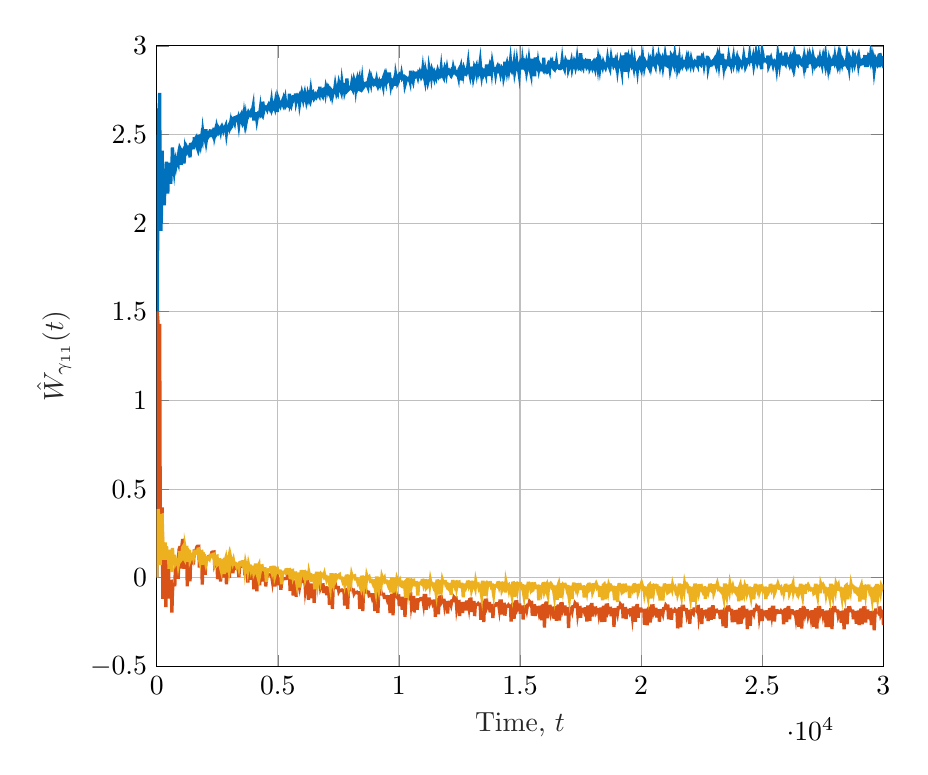
\begin{tikzpicture}

\begin{axis}[%
width=0.761\textwidth,
height=0.65\textwidth,
at={(0\textwidth,0\textwidth)},
scale only axis,
xmin=0,
xmax=30000,
xlabel style={font=\color{white!15!black}},
xlabel={Time, $t$},
ymin=-0.5,
ymax=3,
ylabel style={font=\color{white!15!black}},
ylabel={$\hat{W}_{\gamma_{11}} (t)$},
axis background/.style={fill=white},
xmajorgrids,
ymajorgrids
]
\addplot [color=mycolor1, line width=1.2pt, forget plot]
  table[row sep=crcr]{%
0	0\\
22.0010141601306	1.33620324729054\\
40.006214029152	1.94506876901505\\
58.4816655603645	2.25052123505156\\
78.6879773681503	2.64746859972729\\
100.575489070172	2.612298679589\\
123.3101701749	2.73383489918706\\
146.228660635523	2.00993264494537\\
172.199381604511	1.95709862899821\\
199.216871204237	2.0744386695842\\
226.142061781371	2.40868397178929\\
253.772297893262	2.15840531550566\\
282.213017586499	2.15618423538399\\
312.89006128988	2.10103120912754\\
347.705056364881	2.24430432921872\\
380.612079327715	2.28012010437669\\
405.795319896417	2.34638471990911\\
430.056255439333	2.27174876560821\\
458.369849905459	2.16644201150848\\
488.768333195454	2.33987047767005\\
513.0021832854	2.31245495214171\\
533.191880132432	2.31496521138615\\
554.687533079377	2.33927749259601\\
578.451772799926	2.22136062649588\\
603.376074201657	2.29118876920256\\
628.00477153439	2.32503283415281\\
649.79506491033	2.42657604585838\\
696.193267098693	2.32937716893503\\
720.364412559302	2.29954962929332\\
749.284382873229	2.33926407833133\\
776.20512120143	2.35483854407721\\
802.007542783762	2.33041915704598\\
831.034487188055	2.35390013132928\\
861.011764461884	2.35138989713596\\
889.0061174537	2.33971059514806\\
920.244393502478	2.40472511756525\\
950.83492014186	2.4246156690424\\
981.77304821838	2.41581001038503\\
1011.22772520844	2.32912732452314\\
1039	2.37521645457309\\
1067.04456274024	2.40068314644304\\
1097.98588926185	2.40916451496378\\
1126.78319450584	2.33585145057805\\
1170.14953634024	2.40756568087818\\
1192.34529951866	2.38945672761838\\
1215.36345701218	2.39011681886768\\
1239.8968705598	2.42699697030548\\
1262.33614018248	2.42082023933835\\
1282.68327601124	2.40856835283194\\
1303.59919283675	2.41304790814684\\
1327.34096635567	2.42071919018417\\
1352.02516904102	2.4056446817267\\
1376.70631738191	2.37072613243072\\
1402.94658055512	2.45248228159471\\
1429.24933502657	2.42823318735464\\
1459.17708984501	2.44274687956568\\
1490.00099732692	2.44942572781292\\
1516.23387788289	2.41706438629262\\
1550.66668012608	2.47405695576163\\
1582.75625540383	2.47299352376285\\
1616.81593034523	2.48017740850992\\
1648.20604414454	2.43987453125737\\
1676.02078559775	2.42774569927133\\
1705.57737457926	2.48780608685047\\
1736.39258040744	2.48928401012745\\
1763.07560540824	2.43990793931152\\
1785.71468998064	2.45273729076507\\
1808.05797066675	2.43953002080889\\
1832.20716207739	2.46083717952934\\
1857.12788227338	2.4871630184316\\
1881.99763103162	2.47350280168394\\
1903.76326242409	2.51071293304267\\
1925.86568708504	2.48685320221921\\
1949.69343372955	2.48919900903638\\
1975.51143158512	2.49036932188028\\
2002.65543040722	2.47316562006381\\
2029.54720384807	2.52936390951436\\
2058.40404100144	2.47631084399109\\
2087.82811499125	2.50267915193035\\
2119.21018741299	2.5065832965156\\
2147.60974244864	2.49190879211164\\
2179.22821710862	2.49892404484854\\
2212.00087655821	2.51988954691842\\
2248.27470887678	2.51917005365613\\
2275.31002342947	2.49895918127368\\
2304.04067707442	2.50207527618113\\
2335.00461398508	2.49132959268536\\
2367.15670494568	2.5376556650117\\
2392.07469832007	2.49664623378339\\
2414.93507765002	2.51183424001647\\
2438.21205209333	2.4952252177136\\
2462.86399788344	2.49966999411117\\
2489.54102798222	2.54003515200748\\
2512.87867535083	2.5286028695009\\
2535.76902775786	2.53367285610511\\
2559.03789619781	2.52194918804162\\
2583.08717427489	2.5319563903322\\
2610.55031994384	2.53169483284\\
2636.31609578053	2.51687938375471\\
2663.7054471777	2.54084841432996\\
2692.54660604851	2.54778876651835\\
2725	2.53797508922798\\
2753.26802134881	2.52318824283429\\
2783.80568827383	2.53718692105031\\
2814.76898850397	2.53588012186083\\
2849.73400486278	2.54780049532928\\
2880.88097628015	2.5091651440307\\
2909.70441151558	2.53729196799395\\
2939.34543624319	2.53655679408257\\
2970.07801066419	2.54560485894035\\
3001.88819517193	2.53329897755975\\
3025.18012683544	2.54530183209863\\
3049.88755532052	2.56433416579966\\
3072.70264648159	2.54078244990524\\
3096.00359725381	2.5451280452362\\
3123.7245572495	2.58549070448498\\
3146.00685317941	2.58185703331401\\
3168.56515246117	2.58600215052502\\
3192.17104143348	2.5800516136369\\
3217.22937795712	2.56873495910622\\
3244.95249248798	2.59552670005723\\
3273.0046193674	2.59708686462545\\
3300.94222580976	2.5803293697245\\
3329.29257993141	2.57974252964777\\
3360.82950483446	2.5926562754903\\
3392.16392443045	2.55838739844694\\
3425.37713991607	2.59683011217203\\
3456.05888044651	2.60270388997378\\
3489.02087292794	2.61176046351829\\
3520.98328634123	2.57296785651488\\
3551.62247646616	2.55961957114778\\
3579.34357965102	2.56622452208103\\
3610.37836927607	2.60689743063631\\
3640.53774637625	2.57444630053942\\
3666.50400010544	2.59808048625564\\
3690.46373933997	2.56750278923573\\
3714.44523585703	2.58591804430034\\
3740.21303904782	2.5927677598047\\
3765.57874719471	2.6160225360145\\
3789.5000012821	2.62591046749731\\
3813.41854503588	2.6204790179072\\
3838.02589677472	2.60575822669853\\
3865.14487520794	2.60504048818984\\
3893.08800109858	2.61529156373217\\
3922.48070699275	2.63423719042476\\
3950.32685173723	2.63259384390403\\
3980.91924208061	2.65569992161909\\
4010.93781687778	2.57896178265582\\
4041.00742618711	2.61229774660751\\
4074.62788696224	2.61687308071487\\
4104.76099217656	2.6167305756062\\
4135.52411753067	2.58364816652102\\
4164.84363872227	2.60773390206305\\
4191.67724116229	2.61693413965986\\
4220.34181600386	2.61374652889572\\
4251.88666221631	2.61561100058316\\
4277.8975024907	2.64265600929866\\
4302.65307642276	2.60965069484155\\
4326.35727686555	2.61335316033365\\
4351.12609962662	2.60861252555696\\
4378.45967308257	2.68495967361014\\
4402.99755749093	2.65897900371056\\
4427.18088671436	2.63816891295573\\
4450.88992534439	2.6524907042658\\
4475.64313726746	2.65594592108391\\
4532.11608990744	2.65146011473553\\
4559.46164014736	2.64226700901418\\
4588.83383393395	2.65889899804097\\
4618.92862381508	2.66679398319684\\
4648.901018774	2.65493774288552\\
4679.10286946986	2.6453774008769\\
4708.28132625591	2.65694262617035\\
4737.59335486815	2.6839771331106\\
4767.63086443802	2.64331065347506\\
4796.09506777138	2.653167136501\\
4822.81141342114	2.64924149071521\\
4850.46800446488	2.66483663468534\\
4878.99670483398	2.65147112879276\\
4903.78169939709	2.67726376250721\\
4928.73021140362	2.65384570934839\\
4952.19546971423	2.64868883889358\\
4976.5756600961	2.62687758470202\\
5003.27888956456	2.70819296991613\\
5028.55203787279	2.69826102029765\\
5053.02400866113	2.6701638448576\\
5076.86278048775	2.66911783937394\\
5101.9766380536	2.66188294538733\\
5129.07743266448	2.67692091364006\\
5157.80285819941	2.67589149867126\\
5185.91979487858	2.68601433588265\\
5215.10248702628	2.67347632677411\\
5244.87984160361	2.69591601009961\\
5275.28244402961	2.68003300132477\\
5305.04877713639	2.69952604718128\\
5335.23733968329	2.66347456792937\\
5365.21927850344	2.67030174889442\\
5395.93401645824	2.67059341483036\\
5426.34678531726	2.66239754587878\\
5453.32913367534	2.65978685573646\\
5481.1166906102	2.72929103177739\\
5510.08629175029	2.67020060553841\\
5534.71107337832	2.67973084795449\\
5560.00225549118	2.66783461041268\\
5583.74501536359	2.68116451312017\\
5609.83735346909	2.684713674862\\
5635.53931474248	2.71194212817863\\
5660	2.71158107035808\\
5684.00326531268	2.70257641852731\\
5707.49671665597	2.70075149094555\\
5733.79545157124	2.73063859194372\\
5760.09513935152	2.68598032699811\\
5787.50469944528	2.70158966466624\\
5815.92577524783	2.71489567103345\\
5844.51149746819	2.70889461351544\\
5872.90032774283	2.71605644808733\\
5902.03078964411	2.67545711353523\\
5932.854312785	2.70184057088409\\
5963.41988993171	2.70810463872476\\
5995.06924468521	2.73215002426878\\
6023.71360667713	2.7154670078562\\
6053.12309724616	2.69596126916076\\
6081.14536412859	2.71413213794949\\
6110.75890227409	2.73117503436515\\
6139.02088856078	2.70732180013874\\
6165.02656000227	2.70839135791175\\
6190.23479392473	2.68597901732937\\
6214.02582533636	2.69889739374048\\
6240.42431496458	2.72506181650169\\
6265.81609611158	2.71098426864774\\
6289.57167888949	2.73854279714214\\
6313.49470315636	2.73742029541972\\
6337.00612441976	2.71774368797924\\
6362.00058271465	2.7445581176944\\
6387.84319157732	2.71576921426094\\
6416.69670851818	2.73314064113583\\
6445.91815529961	2.73713573794521\\
6474.89482951662	2.71847951092423\\
6502.13086356609	2.70240617589661\\
6531.38454646943	2.70830664757887\\
6563.00087664022	2.7215812304712\\
6595.2580995895	2.71341670652691\\
6653.52465348812	2.73351462532082\\
6709.16773213907	2.7193265828173\\
6738.24895692791	2.7691466003489\\
6767.41654065242	2.72953883545415\\
6794.67839846663	2.73391957413696\\
6819.11592911143	2.7217317636896\\
6843	2.71683060351279\\
6870	2.75242159217669\\
6895.64554063634	2.75651969435057\\
6943.2747252336	2.75743904712363\\
6967	2.73734271384819\\
6991.90976691926	2.76475362608471\\
7019.85454724813	2.75016883751232\\
7049.88892602786	2.76098288460344\\
7078.03034703268	2.74265825000475\\
7105.0450997172	2.75371570909556\\
7165.20628767484	2.72545791230732\\
7198.96597779813	2.75230607798949\\
7227.8895480703	2.74791781172826\\
7256.13586903482	2.71872815181632\\
7286.07878349411	2.73749323598895\\
7315.32566513611	2.73725729573925\\
7343.51664217019	2.74693490389473\\
7372.81082181324	2.77690227757193\\
7425.90517858284	2.73442190588685\\
7449.1860656328	2.74473518656305\\
7471.24521644833	2.73699602978741\\
7499.39294272152	2.7687402824231\\
7523.04429107055	2.78953816440844\\
7547.18978972044	2.77630440375651\\
7571.36515524789	2.77911870477328\\
7595.64356987678	2.75411719550539\\
7620.16911782198	2.74283384527735\\
7648.63306268269	2.79036095534684\\
7678.28292029199	2.75930241971582\\
7706.92941380541	2.77549585065572\\
7734.09512718724	2.77788191457876\\
7762.06455622318	2.74088796241631\\
7796.11639457328	2.75763521697809\\
7827.85215716439	2.75738632244611\\
7855.54781153105	2.81583521907669\\
7884.49050533435	2.74804558901451\\
7915.04603274785	2.75228244475875\\
7944.97459151303	2.76580685751105\\
8000.20051690676	2.76212079678953\\
8025.24128760182	2.7595597426407\\
8050.71981864595	2.78266833182352\\
8073.4108273489	2.7621990631269\\
8096.86391217875	2.75466134755698\\
8125	2.77989563860319\\
8150.27806551976	2.80484131581397\\
8173.37481975988	2.79337113445581\\
8197.71056301703	2.7957788328531\\
8220.70994001865	2.76324997376287\\
8245.54108682131	2.79260352395795\\
8273.75847969247	2.80800612531675\\
8303.01769658209	2.78007178646294\\
8358.30361291683	2.80986694716194\\
8386.03109157838	2.75233851633675\\
8420.73851300205	2.75046652977471\\
8452.9694793095	2.77262141778556\\
8480.00533694809	2.80352525429771\\
8509.1960041915	2.76083210858633\\
8538.13866858349	2.76666532764648\\
8568.57877024686	2.78238577575758\\
8596.01359391017	2.77928625187269\\
8625.2225427878	2.78705567763973\\
8650.33557885922	2.78536568412528\\
8674.80655530921	2.78916341943477\\
8697.67237086323	2.77689371521046\\
8720.90601312488	2.76868364020629\\
8748.51919023621	2.80913141405108\\
8772.87097714111	2.82246412769746\\
8795.86607076198	2.7981231330341\\
8820.25158874039	2.80169955224119\\
8844.4928187413	2.78710926939311\\
8869.33593743871	2.8141140759617\\
8895.9912597712	2.8010032031234\\
8926	2.7919165735766\\
8953.20734732295	2.78605923103169\\
8979.93459639306	2.79627711884677\\
9007.81729726913	2.78954220546075\\
9040.045282482	2.78515675120434\\
9075.52207723869	2.80757067701052\\
9104.1511688793	2.78274117897672\\
9132.86143558719	2.77178719943913\\
9192.43610570643	2.79708604819461\\
9220.53578756602	2.78477594331343\\
9249.90714044826	2.80156278588765\\
9274.47252934429	2.80295397249211\\
9298.8868417866	2.8059406304601\\
9345.85712704332	2.77651628591411\\
9372.86747478923	2.82410652676481\\
9397.15597424958	2.83342114223706\\
9420.72352081034	2.80611934831904\\
9445.50375354124	2.81731115161529\\
9470.03276370854	2.80049519526801\\
9494.72001503564	2.82742460176451\\
9520.95048670254	2.81432694630712\\
9551.22622921719	2.80337868562128\\
9578.49052189168	2.80773540796145\\
9606.00653581649	2.84886770670346\\
9634.2861894239	2.80998571405507\\
9665.6974778227	2.77947161029806\\
9700.10300010465	2.80845332533499\\
9728.40748189801	2.80549634658746\\
9757	2.783155979203\\
9785.62921761515	2.79199078938836\\
9816.70054209479	2.81017211672588\\
9845.15192750833	2.77532835516104\\
9873.8479973309	2.83297120606585\\
9897.90219557842	2.81509088670282\\
9920.89884936298	2.80973211804303\\
9945.12089641397	2.78832390001116\\
9967.75420076866	2.79457275382083\\
9991.49619615414	2.82871220269953\\
10015.6381273123	2.83491604270966\\
10040.4748984579	2.82759723132767\\
10065.1471262701	2.81897646776997\\
10088.7271597519	2.81771731382105\\
10112.4336380042	2.83824353776436\\
10137.0002924905	2.81935935538422\\
10166.1718921816	2.82559086579204\\
10195.8567315288	2.82757951581516\\
10223.5760787423	2.819238117434\\
10251.721081843	2.78004346367743\\
10281.0559083679	2.79469307665568\\
10312.9771602807	2.81844677605477\\
10345.3478862884	2.81491737188844\\
10375.3874619665	2.81577410389218\\
10402.6362120879	2.81054975666484\\
10431.8095810998	2.81771377259065\\
10460.2986991755	2.80153703446194\\
10487.7856608359	2.85961205645435\\
10514.7886434181	2.81766751904433\\
10538.8136443695	2.82240577097764\\
10586.0005841636	2.80070431712011\\
10609.4964830206	2.82431105329306\\
10633.2591140727	2.84548803100915\\
10659.0853612957	2.84287310160653\\
10682.7111748813	2.84416766273716\\
10706.7608688401	2.83088082421455\\
10754.0603000727	2.8381560279413\\
10782.9061608417	2.82383916377148\\
10811.2851009249	2.84426400245138\\
10838.8122545639	2.83829624105056\\
10866.9759553354	2.85094661814583\\
10897.4814330221	2.83917586674943\\
10928.3126833084	2.82360353708282\\
10958.711617081	2.83131517344009\\
10987.9799728329	2.86576441894067\\
11017.4923231744	2.82803010096541\\
11047.7705521524	2.82951476025119\\
11078.2020763132	2.80784920174119\\
11105.0168981176	2.85348300037731\\
11132.0065355145	2.83498797791617\\
11156.1865977248	2.83229104602287\\
11180.837268897	2.82355024494973\\
11204.007544266	2.79863139650843\\
11226.8567328421	2.81056336135953\\
11250.726882144	2.86986807277208\\
11275.9122181789	2.8514045585398\\
11299.2301155132	2.85372258914504\\
11323.7960983586	2.85902279752918\\
11346.3113295137	2.83208647202264\\
11369.9070264847	2.85887793254005\\
11396.1920568177	2.84693455991146\\
11426.2572232203	2.83538235121159\\
11453.8759103667	2.82119223644258\\
11480.0011726298	2.84538066011737\\
11507.3670018857	2.83584429945404\\
11538.720233748	2.8222097536418\\
11570.9466442886	2.84372173287193\\
11600.6634840819	2.86019013333862\\
11629.2552327251	2.84588092624108\\
11659.0032659006	2.82850013565985\\
11689.6948229364	2.83589497524008\\
11718.3809448164	2.83595739976954\\
11746.5537039263	2.87055634969875\\
11771.215167891	2.83605308413462\\
11796	2.84031510348359\\
11820.3638618617	2.83064859257138\\
11844.2096572353	2.82370706470465\\
11867.0997540751	2.85740327880194\\
11891.9613852194	2.87213041952054\\
11916.4034631606	2.85942691170931\\
11940.983824851	2.86503440763772\\
11964.2687183622	2.84536153166118\\
11987.6605741644	2.86691014417374\\
12012.5155860812	2.84572991697132\\
12070.8657044134	2.85770713644524\\
12125.438981148	2.84074474700174\\
12154.4890639786	2.85192206291686\\
12185.1733878168	2.8382943936449\\
12215.0009897092	2.84787903318647\\
12246.0127866337	2.87581763013804\\
12275.6869599745	2.85780219308072\\
12304.7055308943	2.86415427899919\\
12333.4796243527	2.84509827386864\\
12360.1718877862	2.84165164516526\\
12387.0208345802	2.85281955744722\\
12411.6367051249	2.85130598935939\\
12436.6726366018	2.84196480911123\\
12459.9695211232	2.82671629339893\\
12483.4328512503	2.8668870976071\\
12508.4831068864	2.87329765950562\\
12534.136852221	2.86809277078646\\
12556.6862208933	2.87936217107926\\
12580.8165474457	2.84563372338744\\
12604.5628662644	2.80451208371232\\
12628.5285925226	2.87348707577621\\
12658.1267128354	2.84643006147962\\
12685.9559345771	2.87151597089178\\
12713.2828198036	2.86038207375168\\
12740.1682852228	2.84170887976143\\
12770.5986287998	2.83958804891154\\
12802.8282503582	2.85201514366781\\
12831.4493927615	2.86570346059307\\
12860.9340644743	2.89813323367707\\
12891.0928447515	2.85351609605277\\
12921.255739756	2.85034382324011\\
12951.5574989548	2.82887240950367\\
12978.4998523276	2.84808820812032\\
13005.6533107439	2.87390522044734\\
13030.331662239	2.87433118739864\\
13055.5290164713	2.855712664561\\
13078.9713339615	2.82235156508614\\
13102.3774084584	2.83726007875521\\
13126.80134148	2.8774279524514\\
13151.266115007	2.86940780481746\\
13174.9019137353	2.87336559151663\\
13199.1301084555	2.88268981967849\\
13221.9456253719	2.85595079220366\\
13245.9125869108	2.87797035864423\\
13275.2974756981	2.88281498806828\\
13303.2383107863	2.85989995787531\\
13330.7232666123	2.87805775679226\\
13356.5705521864	2.90607007405924\\
13383.9712257909	2.86319630809885\\
13415.677459534	2.83318541050539\\
13448.1312588489	2.8658187279616\\
13477.7680655411	2.86139700187778\\
13506.0426017832	2.84096957048314\\
13562.4580067404	2.85886472454513\\
13590.7969318192	2.84301673658774\\
13620.0278190022	2.89456564922875\\
13644.9935447296	2.86319903931144\\
13669.6292157111	2.86188265962119\\
13693.5466780383	2.85485818391317\\
13715.8071302804	2.830265315406\\
13739.7556463961	2.87895245619075\\
13764.1705494564	2.89293988938152\\
13788.1842489238	2.88290168378444\\
13811.6959168231	2.88948992096266\\
13834.489442061	2.8633035236453\\
13857.4897628536	2.89865884244864\\
13882.7349200257	2.87806630079649\\
13911.7406837453	2.8687489922886\\
13967.7383360001	2.86998440957541\\
13995.1684381262	2.84287186316578\\
14025.2338670158	2.86948519751604\\
14055.7406594169	2.87842051586631\\
14084.884685574	2.84545872188755\\
14114.5912768317	2.8983595819227\\
14143.4384205957	2.86617149220911\\
14172.8056370825	2.86476748506539\\
14201.415634691	2.84309527235382\\
14228.5361710052	2.8605816225936\\
14256.5731685873	2.8750810242891\\
14281.3875404111	2.87020809781461\\
14306.9133754123	2.86237640554828\\
14329.5663184	2.8271127071821\\
14353.2580536511	2.84224467764216\\
14377.1570571788	2.91063942166511\\
14401.8209138554	2.87187633488793\\
14449.1645716421	2.89455330832789\\
14471.2388082612	2.86554243718274\\
14495.4914969554	2.88540489676234\\
14525.1420207213	2.89362601901303\\
14551.9577947941	2.86466665621992\\
14580.2024648846	2.88606950458416\\
14605.9629734741	2.91523123573643\\
14633.6273769202	2.87216813628766\\
14664.85934408	2.86146084096981\\
14696.5063819466	2.87782946471998\\
14726.9783652478	2.86560234919671\\
14755.2192682638	2.89707637493484\\
14783.3056386544	2.85421821014097\\
14810.9548953555	2.87472070568765\\
14839.4735995488	2.87248329054637\\
14868.5099101597	2.90565437165787\\
14894.3433408788	2.87424304258093\\
14919.6326456098	2.87250875546306\\
14943.1590111958	2.86606239305547\\
14965.7274326144	2.84425627033124\\
14989.3641727455	2.89146342146341\\
15014.3294044259	2.90289465884416\\
15038.0772052373	2.89266200484053\\
15062.1776645775	2.90039748202616\\
15085.3632902977	2.8658333004023\\
15108.7433912122	2.90862723633472\\
15133.0316545838	2.88389554409878\\
15161.8009549125	2.87849943864785\\
15191	2.89542560337213\\
15219.0092411525	2.88005763215915\\
15246.7735819563	2.89784009331197\\
15277.1352852273	2.85689890409776\\
15307.6677756988	2.87869172079081\\
15337.2443107477	2.88198637184178\\
15370.0104251555	2.91764035728556\\
15397.194967148	2.88772962070288\\
15427.1826020863	2.86388322009225\\
15454.0704976149	2.84564601074817\\
15481.395200234	2.927312712618\\
15509.2076279008	2.87289520567356\\
15534.1167957046	2.87465633894317\\
15558.7139915151	2.87041155411134\\
15581.1003785149	2.8586278339244\\
15604.5834425486	2.82802842558158\\
15628.8448444191	2.934505443136\\
15653.9347506205	2.90628713676415\\
15677.0615609375	2.87719485206253\\
15701.4247928756	2.8779658166568\\
15724.6825486649	2.87210363845224\\
15747.9520497777	2.901116377383\\
15777.020646434	2.87300920223061\\
15804.5298903839	2.89526724189272\\
15860.0109582337	2.87880513978598\\
15888.1557755691	2.86820975251612\\
15920.8917272547	2.87234388071738\\
15952.0345566075	2.86568965689003\\
15981.538122626	2.93336165444998\\
16010.8065594949	2.84495602365496\\
16041.0255862117	2.87620891728147\\
16070.2172722494	2.86769197929971\\
16098.0277957288	2.86987786220925\\
16126.785020362	2.88067402372326\\
16151.4728139407	2.85555851406025\\
16176.3429851375	2.85868915596075\\
16198.3689235713	2.87682232780935\\
16221.3721908456	2.86484545155326\\
16245.945218859	2.9013700095893\\
16270.5953929757	2.91029731331582\\
16294.2798193255	2.89862951956457\\
16318.0725116342	2.905680573258\\
16340.67096354	2.87543005197585\\
16364.0021891982	2.91342055445057\\
16390.1470973242	2.87184954516852\\
16420.8023746857	2.86728401269283\\
16451.0556118142	2.8883574118081\\
16477.5973141391	2.88377742402372\\
16504.9108336506	2.90716236983644\\
16534.5212148143	2.87877603386733\\
16565.5304922078	2.87884572736948\\
16598.8016180805	2.88224433166761\\
16628.1967593287	2.87232297167793\\
16657.1931626649	2.87140397431358\\
16685.2023858603	2.87301552849385\\
16712.6763810837	2.88405814455109\\
16741.8931368275	2.91857093445651\\
16768.8612150588	2.88714054856246\\
16793.4788901552	2.88542635759222\\
16816.0534819271	2.87889788893153\\
16838.9793480109	2.87042351296986\\
16862.9833444179	2.89784336779849\\
16887.5265756772	2.91620158398291\\
16934.3762936502	2.90006499139054\\
16957.9615132919	2.89426680255201\\
16980.9287698765	2.92186267503712\\
17005.8539722484	2.86926140534342\\
17035.8495352092	2.88305157643845\\
17065.781146127	2.8912394104118\\
17093.0068573718	2.89179776252058\\
17121.754533053	2.9099748239496\\
17152.2018283804	2.87549354695875\\
17182.0594295384	2.8956572210227\\
17213.1815621645	2.88949867585325\\
17245.446276493	2.91252470927066\\
17274.7984762561	2.90282275140635\\
17303.1286475359	2.88100800483153\\
17330.2756150421	2.89556482885746\\
17358.2693719431	2.92526139465554\\
17386.3975610482	2.89316855599463\\
17411.0069076296	2.88802038953509\\
17434.7238648063	2.87373977346579\\
17457.108789933	2.8761752466562\\
17480.0842295621	2.87342602588251\\
17505.0828694087	2.95833297190984\\
17529.3514683359	2.92510177455188\\
17552.0134652983	2.88753849749264\\
17576.7001548562	2.88678246564814\\
17600.0023503888	2.87916653479624\\
17624.0046220503	2.91123573640652\\
17652.4554845402	2.90677049782244\\
17680.8323722937	2.9118990975403\\
17708.150632174	2.89704409132173\\
17735.3185641035	2.90338024675293\\
17763.56400634	2.8811208916668\\
17797.016465427	2.88827348411724\\
17827.8144537821	2.88125816500906\\
17858	2.92477239048458\\
17887.4075925319	2.8766279028423\\
17917.0090322203	2.88671644048736\\
17946.0062103847	2.89283837180119\\
17974.1691589159	2.88177007899867\\
18002.7254676898	2.90379016239604\\
18027.8101805291	2.90896553518178\\
18052.1738459832	2.88194172672956\\
18074.2747532657	2.88639419787069\\
18096.9958707284	2.87527831088664\\
18122.2102461317	2.9134746822092\\
18145.9882358695	2.91804688613774\\
18169.113120784	2.90841074493073\\
18192.6440738411	2.91576877544139\\
18216.0415658966	2.88845452219903\\
18240.0021974845	2.92439056674993\\
18266.384353786	2.90563928583651\\
18295.7897411507	2.87548585568584\\
18325.0311694252	2.90869568479684\\
18351.1122495609	2.89470393026568\\
18378.8699457833	2.89687925878388\\
18410.1274116481	2.88212155017754\\
18441.1020676679	2.90537747728013\\
18473.8987137187	2.89195544444738\\
18530.9690073923	2.87569439601793\\
18559.0378855896	2.88957230703818\\
18586	2.89274876622585\\
18615.5714323204	2.92330937005681\\
18642.8464521891	2.89628494680437\\
18668.0135147367	2.89396079245489\\
18690.6646509274	2.88222796082118\\
18713.0048108393	2.87325640538984\\
18737.0110628941	2.90558190469892\\
18762	2.93069135663609\\
18785.6569282122	2.91109693724502\\
18808.3481800664	2.90937118612419\\
18832.7609698958	2.90072121560297\\
18856	2.93056188922128\\
18881.2388762852	2.88549848151888\\
18910.3390336443	2.88770798435871\\
18940	2.90807920691441\\
18965.828677836	2.89205834178574\\
18995.8182342013	2.90986273207091\\
19026.8933326186	2.86984845691768\\
19057.1404065991	2.90343055128324\\
19087.000877914	2.90406530893597\\
19120.1451684005	2.89422913658564\\
19148.3710327109	2.9129108237139\\
19203.9233202104	2.86442159993749\\
19231.6143828844	2.94604425701255\\
19260.2175000999	2.89657250281743\\
19285.024269758	2.89050589390536\\
19308.7938219681	2.89064511239849\\
19331.1211128609	2.87770552124493\\
19354.2975650169	2.85397007851134\\
19379.7347567497	2.96172243755791\\
19404.7134473162	2.93905664417252\\
19427.1733183914	2.9053262257039\\
19451.1555803121	2.91148853689447\\
19474.8768779387	2.88745692638258\\
19499.0321768979	2.91867470839134\\
19527.8932173981	2.89824634778051\\
19556.8778384953	2.91636664745965\\
19583.7140697174	2.9054181434949\\
19611.52170378	2.93019467388876\\
19641.5831695434	2.89273072695505\\
19675.5244845488	2.90187588508707\\
19704.3547978078	2.87889253050889\\
19734.1929729785	2.91035415247097\\
19764.4646903608	2.88359021957876\\
19794.7368252292	2.89383072211785\\
19823	2.89792175569528\\
19850.1674720539	2.86694193198491\\
19878.2830113884	2.90732655167449\\
19903.1948038953	2.91424265630485\\
19927.6261840254	2.88658587082682\\
19949.7780582885	2.89213571675646\\
19972.261740706	2.88264366784642\\
19997.9334846695	2.92049400732867\\
20021.9134510645	2.93137117454171\\
20045.1562763557	2.90012648055199\\
20067.492799671	2.92283585761106\\
20090.7017011282	2.88902243160555\\
20114.7423141378	2.92625415975635\\
20140.8222802608	2.88652747380547\\
20171.9621295207	2.90867412229272\\
20201.2605662048	2.89911163218494\\
20227.2832062315	2.90193608216214\\
20255.6997318595	2.89297338684264\\
20286.8548914897	2.88566318424273\\
20319.2584301617	2.91242820582556\\
20349.7580938724	2.88955122527841\\
20379.191284371	2.90749272084213\\
20407.8971142185	2.88374161751926\\
20436.5504507483	2.90410767213325\\
20464.159705265	2.90096603815618\\
20493.6825172191	2.9343695842872\\
20519.8580519221	2.90295482773945\\
20544.346668614	2.90022679980393\\
20566.7333416876	2.89493475148993\\
20589.6154201919	2.88595378177342\\
20613.8004751335	2.91939092744724\\
20639.002184571	2.93254733083813\\
20684.563545512	2.91479715198147\\
20708	2.90903926685496\\
20730.980467321	2.93663692299015\\
20755.6801579311	2.91914898153482\\
20785.2384644385	2.89218638115926\\
20815.3598074557	2.91514225325591\\
20840.8595656164	2.90227445334313\\
20870.7253095709	2.91710283172506\\
20902.1612640542	2.88585010206953\\
20931.3264340366	2.91345530105536\\
20961.2297979928	2.90956672608809\\
20994.0182029041	2.94420737864857\\
21052.7071308584	2.88979629980531\\
21079.9056418274	2.88737410230169\\
21107.0097902397	2.94526835202123\\
21135.2546177424	2.90545038721029\\
21182.411577734	2.89521339731436\\
21204.3643753374	2.8673707042326\\
21227.8168186376	2.88298840350762\\
21253.0273905046	2.9461463126172\\
21277.4258184752	2.94092278758399\\
21300.8074865441	2.91946169558651\\
21323.864380598	2.9290675106713\\
21346.1690303694	2.8976235868904\\
21370.1651190634	2.88763298085178\\
21398.9066495408	2.93715389828867\\
21428.343539206	2.90519812990533\\
21455.1205657992	2.9130438692664\\
21481.8252842627	2.94536586245522\\
21510.6977755172	2.8762753003648\\
21544.7947207753	2.89599085566078\\
21575.4123758837	2.92329252579293\\
21604.444208453	2.87836486942615\\
21635.1577173304	2.88971970259445\\
21664.8867823646	2.8900989402282\\
21693.3310105	2.9083890836082\\
21720.463179188	2.88925439223749\\
21750.1153650781	2.89892856822553\\
21774.8078555814	2.91006370721516\\
21798.6747108913	2.90837966374238\\
21820.5429186501	2.89272895974136\\
21843.1746643419	2.88651288793335\\
21867.9277910391	2.91939255109173\\
21892.4352381078	2.93501770498187\\
21916.6338079603	2.92021966032917\\
21938.722801637	2.92976090014781\\
21961.4078319811	2.90259456980857\\
21985.4633600679	2.91364197997609\\
22010.5877227452	2.91257648705869\\
22040.4255038917	2.89494971527529\\
22070.8935941705	2.92255518340244\\
22097.0199964571	2.9073463381319\\
22126.010750341	2.90051525998933\\
22156.7543914165	2.88632313546623\\
22185.8441492491	2.90556699549779\\
22216.8052825797	2.91208900477432\\
22250.6716787614	2.9056439373926\\
22278.2241326767	2.89755008797511\\
22306.812491607	2.90538294193539\\
22334.0260371876	2.89482346821387\\
22361.3289898076	2.94445319055376\\
22389.8083203582	2.90268530914909\\
22413.695659586	2.90494867232337\\
22436.2630625386	2.8973881161437\\
22458.5658484209	2.89434095545948\\
22482.2685834444	2.92093213905537\\
22507.11702482	2.93325523414751\\
22532.0197612683	2.9255084798715\\
22554.5790502935	2.9342933234002\\
22578.4741394584	2.91761645075894\\
22601.9070106313	2.89427880871153\\
22625.6827884191	2.91470026809475\\
22654.7638888237	2.91600686620222\\
22684.4076349532	2.91184650697323\\
22710.7677477311	2.90496529321535\\
22739.4570755265	2.94316975549737\\
22770.8230271961	2.87900750505287\\
22801.0158882327	2.9008687141868\\
22830.1695816702	2.91280937718329\\
22860.2114887462	2.90393533354654\\
22890.8544211917	2.89118951781711\\
22920.6378515918	2.89217451570585\\
22949.2559566176	2.91101625715964\\
22975.8026610568	2.91660951645463\\
23004.2401238047	2.91733805421973\\
23029.0037727216	2.92316543173729\\
23052.8150711273	2.9005770062322\\
23074.9659016501	2.90051695825605\\
23097.5967481729	2.890579005154\\
23122.991354983	2.92822701508703\\
23147.6895397034	2.94272098005604\\
23171.3632244564	2.9189186436779\\
23195.3343479609	2.93154223603415\\
23218.4158634391	2.9025561692979\\
23241.6229597534	2.93011769482837\\
23270.6833116223	2.90286458518312\\
23301.4107889625	2.90199090425085\\
23328.6613768868	2.90743869439757\\
23355.675568748	2.95521566442039\\
23384.6414632861	2.91617913393929\\
23415.5052193998	2.88131139059988\\
23447.8406826391	2.91585009327537\\
23478.0075391317	2.91282050437803\\
23508.1229602769	2.88805121306723\\
23536.6359696401	2.89652646593095\\
23565.0288488763	2.90790043871675\\
23592.8510128588	2.90310588233842\\
23622.5932477468	2.93576691170529\\
23648.2075357767	2.91627057273217\\
23672.0823056826	2.91058640592018\\
23694.3835626881	2.90190996015372\\
23716.1491956542	2.8901580389429\\
23740.3816979341	2.91633691678726\\
23790.1410748871	2.91462790609876\\
23813.7347444452	2.9334715615696\\
23837.407162001	2.90345366798647\\
23860.8354377281	2.91717810783302\\
23887.53541793	2.91249541826619\\
23918.0073610901	2.91426819201661\\
23947.3731162697	2.92866089402742\\
23975	2.89625899082239\\
24002.9586518565	2.91277421087943\\
24033.5991782584	2.89214363262727\\
24064.0209349202	2.91632682899217\\
24127.5008392399	2.89931022159362\\
24155.9032987803	2.88993936982297\\
24184.6464932265	2.90505994947307\\
24212.2049268531	2.90910348034231\\
24240.6313071896	2.93771254533203\\
24268.907801419	2.91090788687507\\
24293	2.90800278054303\\
24315.1523071887	2.88233711926659\\
24337.0773350261	2.88953795234193\\
24360.9534522977	2.91576194146182\\
24385.7801374151	2.91214604046399\\
24410.5756919431	2.92271632631309\\
24433.5850651256	2.92469833216819\\
24458.00653137	2.91663839107423\\
24481.3220742045	2.94410520793099\\
24506.9021076959	2.91228529147338\\
24536.0034689854	2.91351306310025\\
24565.4219522983	2.91875614121091\\
24592.2106913982	2.91321364606119\\
24622.0276197277	2.93251222998879\\
24652.8079729589	2.89539386357865\\
24681.7260128992	2.91961152964359\\
24712.0002923403	2.91734558614189\\
24745.0003605345	2.95177568381041\\
24773.0877959342	2.92291425132498\\
24803.0819735537	2.90346409682752\\
24830.9358139663	2.91580756875919\\
24858.3469142109	2.94539380888455\\
24887.208792067	2.91272395636406\\
24911.126905121	2.90885102873654\\
24934.2236096488	2.90049102289413\\
24956.047963581	2.88953619761014\\
24979.2248683726	2.86855782024941\\
25004.2429782458	2.96665360705811\\
25029.771340151	2.94891994182763\\
25052.8140399396	2.91824081710729\\
25077.7019424257	2.91485300898057\\
25100.9674355449	2.91456775736515\\
25125	2.92170067751431\\
25183.7025032475	2.91804262839287\\
25210.847948474	2.91083475574487\\
25239.6049397722	2.94562517759186\\
25270.8313806339	2.88619477135217\\
25301.8811087498	2.8968357748272\\
25331.1675345974	2.91918418592832\\
25360.3352989627	2.92987754668138\\
25391.0244931997	2.91169882653048\\
25422.7644757597	2.9076657482874\\
25451.1912289425	2.8912245085412\\
25477.8078372828	2.90670914929069\\
25506.2891170132	2.91395825614381\\
25531	2.90999199912767\\
25554.5194624649	2.90255611893735\\
25577.362493523	2.89839163828947\\
25600.1752193124	2.87445368013141\\
25625.2483002852	2.90670646394574\\
25650.4564802937	2.94862476258641\\
25673.7952164675	2.92848488231539\\
25697.8779608736	2.93379306254064\\
25721.0755831689	2.90488857349919\\
25745	2.93335204530013\\
25774.580193739	2.94190619548681\\
25803.8621530794	2.91636436352564\\
25831.734193303	2.92525443132763\\
25859.1170876986	2.92891772848816\\
25888.0669005408	2.89937206001559\\
25920.8874179873	2.90182187437676\\
25951.8967485151	2.89619597059936\\
25980.5357541766	2.96184448040731\\
26010.9434604763	2.90456514791367\\
26041.4388677881	2.90621588080467\\
26071.1575351125	2.91393447282462\\
26098.9370475038	2.90353114498066\\
26127.624095011	2.92639861672069\\
26153.6018979174	2.9349014941472\\
26177.6346572914	2.89739100520455\\
26200.0057624306	2.90468537179549\\
26222.3049998102	2.89461047061559\\
26246.9586929644	2.93131343311688\\
26271.8341911647	2.94157333279873\\
26295.8163534673	2.90701495799294\\
26319.5330903701	2.93465901144737\\
26342.4639506703	2.90659894128839\\
26365.9724299218	2.93434524589247\\
26395.6226380362	2.91502620586107\\
26426.7359452704	2.90390316265621\\
26454.5888902532	2.89832301960632\\
26481.9072134605	2.95146908107927\\
26510.5455701932	2.90216232998864\\
26542.5069271121	2.9034905242188\\
26575.2133495083	2.91446950221507\\
26604.0226127522	2.89949030681237\\
26634.0098008162	2.89470326815717\\
26665.0015809298	2.89886881858911\\
26693.1808019838	2.91632514753292\\
26720.7454894323	2.8906908756253\\
26750.8681285631	2.93383722219733\\
26776.8503592609	2.91512763621358\\
26801.0323831903	2.89347405067019\\
26823.1594586494	2.90595132831731\\
26845.7870082138	2.87650160733756\\
26870.2907710787	2.91811319336921\\
26895.4406059372	2.94020073502907\\
26919.171338932	2.92692955017992\\
26941.8720668448	2.93510449402311\\
26965.2207302683	2.89608205578043\\
26989.5983556628	2.93988477081439\\
27018.8071056121	2.92502550203426\\
27050.3648356459	2.92952151993086\\
27078.35238074	2.90330533841552\\
27105.170001618	2.93721788287075\\
27134.7631411937	2.91746462228548\\
27165.877472868	2.89927743289081\\
27198.5629782338	2.92091273227925\\
27228.1004255863	2.91599954679259\\
27258.1768927357	2.89214755160356\\
27288.5413338939	2.89698987602969\\
27316.8296678057	2.91675679730542\\
27344.0437179423	2.90713653855346\\
27374.2707254258	2.92738343069504\\
27400.8332275664	2.89919558801193\\
27447.2756616318	2.90661504402669\\
27470	2.89426380423174\\
27494.0279742197	2.9269684804749\\
27518.7227640712	2.94262922373673\\
27542.4774027758	2.92742916224597\\
27565.6125188648	2.93366469513785\\
27589.2036653517	2.91365652983222\\
27613.4081425588	2.93992741034526\\
27640.8169628065	2.89764839851341\\
27672.814612462	2.92133581919916\\
27702.2572520585	2.91630681974493\\
27729.4122386305	2.88300563161829\\
27758.331123271	2.91447728433559\\
27790.4253706992	2.88969818494297\\
27823.0579402056	2.91972394248296\\
27852.6343584113	2.91176375398209\\
27882.2044338566	2.89521197633439\\
27913.0159840651	2.89715269301087\\
27941.4261939574	2.91748235980049\\
27969.0046230115	2.90785359267102\\
27999	2.9355687332536\\
28025.2717268287	2.90860870079268\\
28049.5943498209	2.9160350915954\\
28071.6079319229	2.90679347130572\\
28094.195463607	2.89477031233037\\
28118.0138598519	2.9275572364968\\
28141.7708540616	2.94323797217658\\
28165.8453321901	2.91796174028059\\
28189.1926498465	2.93659775632477\\
28212.8436001935	2.90981648408706\\
28237.0048153584	2.93434194126894\\
28263.9680157547	2.91463419066713\\
28295.7574695805	2.89752841235895\\
28325.9597610187	2.91943758519119\\
28352.747122493	2.91220137187702\\
28381.6544950095	2.89338718723957\\
28413.1823437261	2.89554601412237\\
28445.1861304284	2.90252627013979\\
28475.2003821585	2.89456396227615\\
28504.67220298	2.93733197340407\\
28534.8779283477	2.90230986765891\\
28563.0035030778	2.91100180366993\\
28590.2210291104	2.88355512668932\\
28620.3163183638	2.93005299170909\\
28647.5172895388	2.92022162859212\\
28672.0080921273	2.91522277788681\\
28695.0037430975	2.90710355971896\\
28716.8606718039	2.89527406542402\\
28740.3648696059	2.92071416058752\\
28764.2748698522	2.94260103211127\\
28789	2.93172123700424\\
28812.4038027426	2.9376199673934\\
28836.0018179955	2.9082628989745\\
28860.4259457145	2.92299140892283\\
28886.2105158271	2.91578009584919\\
28918.007374564	2.91882725189498\\
28948.2831430226	2.93241853921063\\
28975.2043063735	2.89921253374632\\
29004.3464674471	2.92628706115283\\
29035.1501329456	2.89967982259259\\
29065.5069865179	2.90842027221515\\
29097.0394349468	2.9128642811811\\
29127.6962994105	2.89861214327539\\
29157.1777404033	2.8995625173884\\
29185.9017541274	2.91619731163519\\
29213.3792088113	2.91326599491003\\
29242.8578737825	2.94730692213852\\
29270.8216166032	2.88033008023558\\
29295.4871441048	2.90712091020032\\
29317.8497330504	2.90753164897251\\
29340.2614827784	2.88125127344028\\
29364.2490920195	2.93097770455643\\
29387.5040172095	2.94358255493717\\
29411.8391524753	2.93830235837595\\
29459.0307215136	2.91523138268894\\
29483.3547858645	2.94864041961409\\
29508.6546911831	2.92217629731022\\
29539.1174895516	2.90818665616098\\
29570.0326877926	2.93484224814165\\
29596.0074511777	2.91380265605039\\
29626.4062091932	2.86318361658414\\
29686.0137636548	2.9251277933181\\
29715.8652035444	2.91627515044456\\
29750.2340285162	2.90289025807215\\
29778.9569935819	2.91930957648947\\
29808	2.90594814837823\\
29835.1646848751	2.87915162519494\\
29863.8334851894	2.95874387675212\\
29892.9633558027	2.91585224363371\\
29917.1866366721	2.91276656727132\\
29940.1038471144	2.89878803391912\\
29962.1547030299	2.89415016302155\\
29985.2265665122	2.90486803116801\\
30009.0032624117	2.94213463809865\\
};
\addplot [color=mycolor2, line width=1.2pt, forget plot]
  table[row sep=crcr]{%
0	0\\
22.0010141601306	1.50151336197086\\
40.006214029152	1.47013207679265\\
58.4816655603645	1.42480048478683\\
78.6879773681503	1.4228227251042\\
123.3101701749	1.42279314429834\\
146.228660635523	0.350737757387833\\
172.199381604511	0.388765745152341\\
199.216871204237	0.386829697257781\\
226.142061781371	0.386835280518426\\
253.772297893262	-0.119198268337641\\
282.213017586499	0.085413231223356\\
312.89006128988	0.121861946350691\\
347.705056364881	0.122915527626901\\
380.612079327715	-0.165480049970938\\
405.795319896417	0.0709558153903345\\
430.056255439333	0.0868462025791814\\
488.768333195454	0.0868175758878351\\
513.0021832854	-0.117078070685238\\
533.191880132432	-0.0244299696569215\\
554.687533079377	-0.0218073810247006\\
603.376074201657	-0.0206032905698521\\
628.00477153439	-0.196156492740556\\
649.79506491033	-0.0853937981919444\\
671.834495370531	-0.0382521538231231\\
749.284382873229	-0.0388000575330807\\
776.20512120143	0.0666007490108314\\
802.007542783762	0.0725411351741059\\
861.011764461884	0.0724373015946185\\
889.0061174537	-0.00610335304736509\\
920.244393502478	0.156853950116783\\
950.83492014186	0.170917837673187\\
981.77304821838	0.170917336592538\\
1011.22772520844	0.0510290756355971\\
1039	0.179950987057964\\
1067.04456274024	0.210313606025011\\
1097.98588926185	0.210649992954131\\
1126.78319450584	0.049930595439946\\
1148.81605766601	0.114031884408178\\
1170.14953634024	0.125794478019088\\
1192.34529951866	0.134197462943121\\
1239.8968705598	0.135063770405395\\
1262.33614018248	-0.0487261417365517\\
1282.68327601124	0.0720475553571305\\
1303.59919283675	0.0785935481835622\\
1352.02516904102	0.077937748086697\\
1376.70631738191	-0.0198681478177605\\
1402.94658055512	0.112926890265953\\
1429.24933502657	0.117154410916555\\
1490.00099732692	0.117211787906854\\
1516.23387788289	0.0744372085246141\\
1550.66668012608	0.150099902668444\\
1616.81593034523	0.150144932849798\\
1648.20604414454	0.169148508877697\\
1676.02078559775	0.176808420354064\\
1736.39258040744	0.17746862619606\\
1763.07560540824	0.0577478664199589\\
1785.71468998064	0.0869953145702311\\
1808.05797066675	0.1209761789396\\
1832.20716207739	0.122773610783042\\
1857.12788227338	0.122781389593001\\
1881.99763103162	-0.039180860730994\\
1903.76326242409	0.0820680330762116\\
1925.86568708504	0.0828994109142513\\
1975.51143158512	0.0820968951884424\\
2002.65543040722	0.0169756811083062\\
2029.54720384807	0.0976216923372704\\
2058.40404100144	0.106627242428658\\
2119.21018741299	0.107070995960385\\
2147.60974244864	0.119347259045753\\
2248.27470887678	0.120715609416948\\
2275.31002342947	0.142225254079676\\
2304.04067707442	0.144969087185018\\
2367.15670494568	0.14553169069768\\
2392.07469832007	0.0772678838657157\\
2414.93507765002	0.0857421629407327\\
2438.21205209333	0.102861172836128\\
2489.54102798222	0.103944814218266\\
2512.87867535083	-0.00820055027361377\\
2535.76902775786	0.0617721435119165\\
2559.03789619781	0.0705912352823361\\
2610.55031994384	0.0708112320608052\\
2636.31609578053	-0.0216968227978214\\
2663.7054471777	0.0702923936041771\\
2692.54660604851	0.0845168185624061\\
2725	0.0846355570356536\\
2753.26802134881	0.00138995814995724\\
2783.80568827383	0.0655028171022423\\
2814.76898850397	0.0909046092601784\\
2849.73400486278	0.091469189930649\\
2880.88097628015	-0.037353067080403\\
2909.70441151558	0.0823147899245669\\
2939.34543624319	0.115378752758261\\
2970.07801066419	0.116200380478404\\
3001.88819517193	-0.000945059910009149\\
3025.18012683544	0.0775355656151078\\
3049.88755532052	0.0829916698567104\\
3096.00359725381	0.081932939698163\\
3123.7245572495	0.0819330844969954\\
3146.00685317941	0.0254055130717461\\
3168.56515246117	0.0529518268376705\\
3244.95249248798	0.0528034394919814\\
3273.0046193674	0.062461591369356\\
3300.94222580976	0.0601741417412995\\
3360.82950483446	0.0603980681444227\\
3392.16392443045	0.00367675761663122\\
3425.37713991607	0.0645037769172632\\
3489.02087292794	0.0645746327390953\\
3520.98328634123	0.073690271765372\\
3551.62247646616	0.0886702623101883\\
3610.37836927607	0.0894505646319885\\
3640.53774637625	0.013712998439587\\
3666.50400010544	0.0518269180174684\\
3690.46373933997	0.0584695413490408\\
3740.21303904782	0.0593267598451348\\
3765.57874719471	-0.0275115505355643\\
3789.5000012821	0.0316511078017356\\
3838.02589677472	0.0331315865114448\\
3865.14487520794	0.0331318960852514\\
3893.08800109858	-0.0106282627275505\\
3922.48070699275	0.0367062997393077\\
3980.91924208061	0.036645231917646\\
4010.93781687778	-0.0656150861686911\\
4041.00742618711	0.0295434974141244\\
4074.62788696224	0.0398408829860273\\
4104.76099217656	0.0398408853870933\\
4135.52411753067	-0.0761835652556329\\
4164.84363872227	0.0387700209976174\\
4191.67724116229	0.0634268661597162\\
4220.34181600386	0.0637975061908946\\
4251.88666221631	-0.0424819749096059\\
4277.8975024907	0.0209383376895858\\
4302.65307642276	0.0358200618247793\\
4351.12609962662	0.0364549540645385\\
4378.45967308257	-0.0210999719856773\\
4402.99755749093	0.00659806487965398\\
4427.18088671436	0.0128903499244188\\
4475.64313726746	0.0127906612724473\\
4502.89300107902	-0.0488057327493152\\
4532.11608990744	-0.00374169246788369\\
4559.46164014736	0.0133914465986891\\
4648.901018774	0.0155278925885796\\
4708.28132625591	0.0172901443584124\\
4737.59335486815	0.0172920991753927\\
4767.63086443802	-0.00904588390039862\\
4796.09506777138	0.0380491099531355\\
4822.81141342114	0.0400577377258742\\
4850.46800446488	0.0400566105417965\\
4878.99670483398	-0.0497327416342159\\
4903.78169939709	0.000545998438610695\\
4928.73021140362	0.0143464211614628\\
4976.5756600961	0.0149347879851121\\
5003.27888956456	-0.0419058241423045\\
5028.55203787279	-0.0131783370088669\\
5053.02400866113	-0.00636683338234434\\
5101.9766380536	-0.00672198416941683\\
5129.07743266448	-0.0678523617316387\\
5157.80285819941	-0.0241167124549975\\
5185.91979487858	-0.00743635069738957\\
5275.28244402961	-0.00532911855407292\\
5335.23733968329	-0.00355882803341956\\
5365.21927850344	-0.00355687534829485\\
5395.93401645824	0.0018526485619077\\
5426.34678531726	0.0177116100676358\\
5481.1166906102	0.0184192602391704\\
5510.08629175029	-0.0735201156348921\\
5534.71107337832	-0.0272913160297321\\
5560.00225549118	-0.00575440006650751\\
5609.83735346909	-0.00480561188305728\\
5635.53931474248	-0.100699094127776\\
5660	-0.0321250804590818\\
5684.00326531268	-0.0247176333687094\\
5733.79545157124	-0.0244461949368997\\
5760.09513935152	-0.107501732851233\\
5787.50469944528	-0.0394277411905932\\
5815.92577524783	-0.0261986733057711\\
5872.90032774283	-0.026079690138431\\
5902.03078964411	-0.0490306371248153\\
5932.854312785	-0.0224882252514362\\
5995.06924468521	-0.0218105591848143\\
6023.71360667713	0.00165137250223779\\
6053.12309724616	-0.00140638446464436\\
6110.75890227409	-0.000706247705238638\\
6139.02088856078	-0.0620512429377413\\
6165.02656000227	-0.0374083589886141\\
6190.23479392473	-0.0241337505176489\\
6240.42431496458	-0.0234682571644953\\
6265.81609611158	-0.124947914107906\\
6289.57167888949	-0.0431679261600948\\
6337.00612441976	-0.0415078074911435\\
6362.00058271465	-0.0415076102763123\\
6387.84319157732	-0.115613897109142\\
6416.69670851818	-0.049509564647451\\
6445.91815529961	-0.0428931466158247\\
6474.89482951662	-0.0428491167222091\\
6502.13086356609	-0.141328210276697\\
6531.38454646943	-0.0662271525579854\\
6563.00087664022	-0.0393047081161058\\
6653.52465348812	-0.0378288231877377\\
6681.66633450691	-0.0194171318180452\\
6738.24895692791	-0.0183382867289765\\
6767.41654065242	-0.0565411225543357\\
6794.67839846663	-0.0468376665230608\\
6819.11592911143	-0.0406731636103359\\
6870	-0.0403443069553759\\
6895.64554063634	-0.0853173121613509\\
6919.88358378213	-0.0576091284638096\\
6991.90976691926	-0.0573293642191857\\
7019.85454724813	-0.098026283118088\\
7049.88892602786	-0.059036669186753\\
7105.0450997172	-0.0588991471850022\\
7133.08220720066	-0.153141599395894\\
7165.20628767484	-0.0748382609890541\\
7198.96597779813	-0.0538723294121155\\
7227.8895480703	-0.0538724209473003\\
7256.13586903482	-0.174837876525999\\
7286.07878349411	-0.0579463764406682\\
7315.32566513611	-0.0349640147251193\\
7372.81082181324	-0.0341969999062712\\
7399.30890412766	-0.0543264723855827\\
7425.90517858284	-0.0560175858518051\\
7499.39294272152	-0.0554217173012148\\
7523.04429107055	-0.0767561428801855\\
7547.18978972044	-0.0707613896229304\\
7595.64356987678	-0.0717512766095751\\
7620.16911782198	-0.0717509655514732\\
7648.63306268269	-0.0694719961138617\\
7678.28292029199	-0.0728239130439761\\
7734.09512718724	-0.0725060974546068\\
7762.06455622318	-0.156474779774726\\
7796.11639457328	-0.0699764459095604\\
7827.85215716439	-0.0671677589161845\\
7855.54781153105	-0.067166155709856\\
7884.49050533435	-0.175702171520243\\
7915.04603274785	-0.0723013334900315\\
7944.97459151303	-0.0488223466527415\\
8000.20051690676	-0.0485076049590134\\
8025.24128760182	-0.06767054588272\\
8125	-0.0689826235866349\\
8150.27806551976	-0.0887175021707662\\
8173.37481975988	-0.0831633319394314\\
8220.70994001865	-0.0842563412115851\\
8245.54108682131	-0.0842559681295825\\
8273.75847969247	-0.0816591504917596\\
8303.01769658209	-0.0851778277683479\\
8358.30361291683	-0.0848667491372908\\
8386.03109157838	-0.174875900713232\\
8420.73851300205	-0.0960555219608068\\
8452.9694793095	-0.0790415750889224\\
8480.00533694809	-0.0790399615871138\\
8509.1960041915	-0.187620073495054\\
8538.13866858349	-0.0844454239449988\\
8568.57877024686	-0.0612107686065428\\
8625.2225427878	-0.0609056056164263\\
8650.33557885922	-0.0799739749236323\\
8748.51919023621	-0.0812599641176348\\
8772.87097714111	-0.100292440230987\\
8820.25158874039	-0.0963498708260886\\
8869.33593743871	-0.0962077403164585\\
8895.9912597712	-0.11034583138462\\
8926	-0.0969716081017395\\
8979.93459639306	-0.0965309122511826\\
9007.81729726913	-0.187998942135891\\
9040.045282482	-0.110904940491309\\
9075.52207723869	-0.09021931641837\\
9104.1511688793	-0.0902194525624509\\
9132.86143558719	-0.1984582427649\\
9161.71712835457	-0.0962670514745696\\
9192.43610570643	-0.073092857030133\\
9249.90714044826	-0.0727966241611284\\
9274.47252934429	-0.0915035648104094\\
9372.86747478923	-0.0930151670363557\\
9397.15597424958	-0.110800079044566\\
9420.72352081034	-0.110346758894593\\
9445.50375354124	-0.10686372499913\\
9494.72001503564	-0.10671922754409\\
9520.95048670254	-0.120908342414623\\
9551.22622921719	-0.107288163562771\\
9606.00653581649	-0.106822892204946\\
9634.2861894239	-0.198892467607948\\
9665.6974778227	-0.12174262102053\\
9700.10300010465	-0.0993627256139007\\
9728.40748189801	-0.0993628674223146\\
9757	-0.212545916347153\\
9785.62921761515	-0.11312684207951\\
9816.70054209479	-0.0828329279829632\\
9873.8479973309	-0.0825349841215939\\
9897.90219557842	-0.101104487668636\\
9920.89884936298	-0.106282044278487\\
9945.12089641397	-0.10293423109033\\
9991.49619615414	-0.102670626249164\\
10015.6381273123	-0.160136643804435\\
10040.4748984579	-0.118281782448321\\
10065.1471262701	-0.116554772783275\\
10112.4336380042	-0.116357406321185\\
10137.0002924905	-0.180351530565531\\
10166.1718921816	-0.121927738411614\\
10195.8567315288	-0.115808696558815\\
10223.5760787423	-0.11568914644522\\
10251.721081843	-0.220576463445468\\
10281.0559083679	-0.138472745074978\\
10312.9771602807	-0.108133770147106\\
10375.3874619665	-0.107690026150522\\
10402.6362120879	-0.110714945760265\\
10431.8095810998	-0.0926611176873848\\
10487.7856608359	-0.0915749270898232\\
10514.7886434181	-0.146634535889461\\
10538.8136443695	-0.124112404257176\\
10563.1712794126	-0.112607463539462\\
10609.4964830206	-0.112068116981391\\
10633.2591140727	-0.195623255654937\\
10659.0853612957	-0.13290570877507\\
10682.7111748813	-0.125339339443599\\
10729.9650921833	-0.125046646309784\\
10754.0603000727	-0.180051490438927\\
10782.9061608417	-0.140785565745318\\
10811.2851009249	-0.124354795869294\\
10866.9759553354	-0.124091187193699\\
10897.4814330221	-0.117308990080346\\
10987.9799728329	-0.116243478041724\\
11017.4923231744	-0.143467835714546\\
11047.7705521524	-0.100055532308033\\
11105.0168981176	-0.100192617544963\\
11132.0065355145	-0.180451869397075\\
11156.1865977248	-0.137409953356837\\
11180.837268897	-0.120977798465901\\
11226.8567328421	-0.11990112159765\\
11250.726882144	-0.119738367648097\\
11275.9122181789	-0.140430418221513\\
11299.2301155132	-0.131428303579014\\
11346.3113295137	-0.13245323269075\\
11369.9070264847	-0.132453280013578\\
11396.1920568177	-0.143916934746812\\
11426.2572232203	-0.132041690048936\\
11480.0011726298	-0.131609750977077\\
11507.3670018857	-0.220551797134249\\
11538.720233748	-0.143935781663458\\
11570.9466442886	-0.123650907244155\\
11600.6634840819	-0.12362341255357\\
11629.2552327251	-0.206321085326636\\
11659.0032659006	-0.138108139050019\\
11689.6948229364	-0.108497384360817\\
11746.5537039263	-0.107779028552613\\
11771.215167891	-0.135130525053683\\
11796	-0.129390146641526\\
11820.3638618617	-0.127582455817901\\
11867.0997540751	-0.127350684262638\\
11891.9613852194	-0.156964157566108\\
11916.4034631606	-0.139995358978922\\
11987.6605741644	-0.139433860076679\\
12012.5155860812	-0.202052061347786\\
12041.5983106503	-0.144642653176561\\
12070.8657044134	-0.138455064578011\\
12125.438981148	-0.138354372506001\\
12154.4890639786	-0.151982959854649\\
12185.1733878168	-0.130479891653522\\
12246.0127866337	-0.129826403404877\\
12275.6869599745	-0.110220473947265\\
12304.7055308943	-0.115197307950439\\
12360.1718877862	-0.114487491020554\\
12387.0208345802	-0.165907638347562\\
12411.6367051249	-0.145134612710535\\
12436.6726366018	-0.134604873692297\\
12483.4328512503	-0.134078593197046\\
12508.4831068864	-0.215576867652999\\
12534.136852221	-0.153607916250621\\
12556.6862208933	-0.146001398225053\\
12604.5628662644	-0.145726413014927\\
12628.5285925226	-0.198739536615903\\
12658.1267128354	-0.161267683048209\\
12685.9559345771	-0.144769458715018\\
12740.1682852228	-0.144541968991689\\
12770.5986287998	-0.184880566717766\\
12802.8282503582	-0.1366380357249\\
12860.9340644743	-0.136087036440586\\
12891.0928447515	-0.162918647820334\\
12921.255739756	-0.122587037676567\\
12951.5574989548	-0.12059485334612\\
12978.4998523276	-0.120591442278965\\
13005.6533107439	-0.193830321444693\\
13030.331662239	-0.151144106679567\\
13055.5290164713	-0.140281137177226\\
13102.3774084584	-0.139885220214637\\
13126.80134148	-0.216671237623814\\
13151.266115007	-0.164340429706499\\
13174.9019137353	-0.150415187981707\\
13221.9456253719	-0.151416835564305\\
13245.9125869108	-0.151416857952427\\
13275.2974756981	-0.145945578919054\\
13303.2383107863	-0.150466837949352\\
13356.5705521864	-0.150151486192044\\
13383.9712257909	-0.237711706959089\\
13415.677459534	-0.162689782828238\\
13448.1312588489	-0.141293056949507\\
13477.7680655411	-0.14129319390122\\
13506.0426017832	-0.249566172489722\\
13534.0065310949	-0.156131137748162\\
13562.4580067404	-0.126806961019611\\
13620.0278190022	-0.126106934454583\\
13644.9935447296	-0.15995967159688\\
13669.6292157111	-0.150719549765199\\
13693.5466780383	-0.145519643141597\\
13739.7556463961	-0.145301128020947\\
13764.1705494564	-0.195369902066886\\
13788.1842489238	-0.158292811098363\\
13811.6959168231	-0.156448385077965\\
13857.4897628536	-0.156283809701563\\
13882.7349200257	-0.227727426005004\\
13911.7406837453	-0.166306562816317\\
13940.7620066004	-0.15491827256119\\
13995.1684381262	-0.154631873119797\\
14025.2338670158	-0.146994125672791\\
14114.5912768317	-0.145830428962654\\
14143.4384205957	-0.172843604901573\\
14172.8056370825	-0.131043970621249\\
14228.5361710052	-0.131139405704744\\
14256.5731685873	-0.206907934807532\\
14281.3875404111	-0.166449644628301\\
14306.9133754123	-0.150811562474701\\
14353.2580536511	-0.150058189457923\\
14377.1570571788	-0.213574177832925\\
14401.8209138554	-0.184572001140623\\
14425.1169722494	-0.159797017251549\\
14471.2388082612	-0.160787705899565\\
14495.4914969554	-0.160787654840533\\
14525.1420207213	-0.154535912515712\\
14551.9577947941	-0.159607539844728\\
14605.9629734741	-0.15898205377016\\
14633.6273769202	-0.247446511519229\\
14664.85934408	-0.169856117736344\\
14696.5063819466	-0.150066172449442\\
14726.9783652478	-0.150033971578523\\
14755.2192682638	-0.231285153149656\\
14783.3056386544	-0.165586704490124\\
14810.9548953555	-0.136369087809726\\
14868.5099101597	-0.135696095294406\\
14894.3433408788	-0.169235429013497\\
14919.6326456098	-0.159667071417061\\
14943.1590111958	-0.154563846310339\\
14989.3641727455	-0.154352224737522\\
15014.3294044259	-0.203432853289996\\
15038.0772052373	-0.166843754792353\\
15062.1776645775	-0.164962085658772\\
15108.7433912122	-0.164790627404727\\
15133.0316545838	-0.236276277661091\\
15161.8009549125	-0.174716311837983\\
15191	-0.163115840594401\\
15246.7735819563	-0.163003605211998\\
15277.1352852273	-0.180581048844033\\
15307.6677756988	-0.154513124100049\\
15370.0104251555	-0.153852630905021\\
15397.194967148	-0.135106783305673\\
15427.1826020863	-0.14015715012647\\
15481.395200234	-0.139400542884687\\
15509.2076279008	-0.213801795242034\\
15534.1167957046	-0.17658141586071\\
15558.7139915151	-0.159199148434709\\
15604.5834425486	-0.158431996453146\\
15628.8448444191	-0.215799528919888\\
15653.9347506205	-0.175806547944376\\
15677.0615609375	-0.168612973990093\\
15747.9520497777	-0.16837617141573\\
15777.020646434	-0.189251593681547\\
15804.5298903839	-0.166746668957785\\
15860.0109582337	-0.166433974089159\\
15888.1557755691	-0.239438350628916\\
15920.8917272547	-0.159256216513313\\
15952.0345566075	-0.156905758594803\\
15981.538122626	-0.156903625629639\\
16010.8065594949	-0.280530924253981\\
16041.0255862117	-0.152072074946773\\
16070.2172722494	-0.143010150350165\\
16098.0277957288	-0.142756012610334\\
16126.785020362	-0.228399797368183\\
16151.4728139407	-0.185271322388871\\
16176.3429851375	-0.162076764376252\\
16245.945218859	-0.161484530279267\\
16270.5953929757	-0.187945888403192\\
16294.2798193255	-0.172082907651202\\
16364.0021891982	-0.171416929581028\\
16390.1470973242	-0.230639022796822\\
16420.8023746857	-0.181537820189988\\
16451.0556118142	-0.169454463859438\\
16477.5973141391	-0.169454017694079\\
16504.9108336506	-0.242533786396962\\
16534.5212148143	-0.186122461240302\\
16565.5304922078	-0.159973156434717\\
16598.8016180805	-0.159555408121378\\
16628.1967593287	-0.240783274588466\\
16657.1931626649	-0.17603345311727\\
16685.2023858603	-0.14714044889115\\
16741.8931368275	-0.146070692215289\\
16768.8612150588	-0.179582633471\\
16793.4788901552	-0.169883291364386\\
16816.0534819271	-0.165086119210173\\
16862.9833444179	-0.164882493012556\\
16887.5265756772	-0.212922034021176\\
16911.0036784575	-0.178753044841869\\
16934.3762936502	-0.174723696316505\\
16980.9287698765	-0.174423762822698\\
17005.8539722484	-0.284131441487261\\
17035.8495352092	-0.187159834033082\\
17065.781146127	-0.172755355324625\\
17121.754533053	-0.172461710411881\\
17152.2018283804	-0.187568439028837\\
17182.0594295384	-0.163269719949312\\
17245.446276493	-0.162639601821866\\
17274.7984762561	-0.144191380226403\\
17303.1286475359	-0.149442317964713\\
17358.2693719431	-0.14873429535146\\
17386.3975610482	-0.200096322845638\\
17411.0069076296	-0.179360150756111\\
17434.7238648063	-0.168521620602405\\
17480.0842295621	-0.167760583393829\\
17505.0828694087	-0.225569848586019\\
17529.3514683359	-0.184651418901922\\
17552.0134652983	-0.177496761454677\\
17624.0046220503	-0.177244866787078\\
17652.4554845402	-0.188935338908777\\
17680.8323722937	-0.175545982114272\\
17735.3185641035	-0.17515916719276\\
17763.56400634	-0.247111841195874\\
17797.016465427	-0.165324922323634\\
17858	-0.165169493491703\\
17887.4075925319	-0.242396889756492\\
17917.0090322203	-0.160324718246557\\
17946.0062103847	-0.151211157299258\\
17974.1691589159	-0.151188705647655\\
18002.7254676898	-0.218949976075237\\
18027.8101805291	-0.18202867664877\\
18052.1738459832	-0.17072712789377\\
18122.2102461317	-0.170323065933189\\
18145.9882358695	-0.188640392821981\\
18169.113120784	-0.18001377589826\\
18240.0021974845	-0.179349219397409\\
18266.384353786	-0.208884481467976\\
18295.7897411507	-0.189574033945973\\
18325.0311694252	-0.177094568731263\\
18351.1122495609	-0.1770948734993\\
18378.8699457833	-0.249889892962528\\
18410.1274116481	-0.193694654371939\\
18441.1020676679	-0.1671841375246\\
18473.8987137187	-0.167048732124385\\
18503	-0.247753000581724\\
18530.9690073923	-0.184277647917042\\
18559.0378855896	-0.154526111986343\\
18615.5714323204	-0.153449703120714\\
18642.8464521891	-0.186724967305054\\
18668.0135147367	-0.177425361740461\\
18690.6646509274	-0.172776549050468\\
18737.0110628941	-0.172253502656531\\
18762	-0.216865686117671\\
18785.6569282122	-0.188991068465839\\
18808.3481800664	-0.181565782699181\\
18856	-0.181264381233632\\
18881.2388762852	-0.277101469117042\\
18910.3390336443	-0.195463133783051\\
18940	-0.178952358081006\\
18995.8182342013	-0.178723386969068\\
19026.8933326186	-0.198399400433118\\
19057.1404065991	-0.169620702567045\\
19120.1451684005	-0.168981931139569\\
19148.3710327109	-0.150249484853703\\
19177.2432220979	-0.155713343752723\\
19231.6143828844	-0.15498719410607\\
19260.2175000999	-0.228552029169805\\
19285.024269758	-0.192127542712115\\
19308.7938219681	-0.174848786009534\\
19354.2975650169	-0.174100777738204\\
19379.7347567497	-0.232563761146594\\
19404.7134473162	-0.191124713201134\\
19427.1733183914	-0.183396873704623\\
19499.0321768979	-0.183369336820761\\
19527.8932173981	-0.19445636058299\\
19556.8778384953	-0.181039979932393\\
19611.52170378	-0.180712214172672\\
19641.5831695434	-0.216796127882844\\
19675.5244845488	-0.170758704105538\\
19734.1929729785	-0.170554977637948\\
19764.4646903608	-0.248201630169206\\
19794.7368252292	-0.166012478788616\\
19823	-0.15697509876918\\
19850.1674720539	-0.156975014739146\\
19878.2830113884	-0.225296748874825\\
19903.1948038953	-0.188028626231244\\
19927.6261840254	-0.176620973641548\\
19997.9334846695	-0.176233345449873\\
20021.9134510645	-0.186818982496334\\
20090.7017011282	-0.18533509781264\\
20114.7423141378	-0.185334672143654\\
20140.8222802608	-0.265582264335535\\
20171.9621295207	-0.183208205849951\\
20227.2832062315	-0.182814275125565\\
20255.6997318595	-0.268008621176705\\
20286.8548914897	-0.191501003748272\\
20319.2584301617	-0.172214637390425\\
20349.7580938724	-0.172080873191589\\
20379.191284371	-0.252996915587573\\
20407.8971142185	-0.188340838984004\\
20436.5504507483	-0.1593782246091\\
20493.6825172191	-0.158710245890688\\
20519.8580519221	-0.192274007782544\\
20544.346668614	-0.182905290355848\\
20566.7333416876	-0.177938192413421\\
20613.8004751335	-0.177748068137589\\
20639.002184571	-0.224593057457241\\
20662.2431619448	-0.188338683747133\\
20708	-0.18680725435479\\
20730.980467321	-0.186806054163753\\
20755.6801579311	-0.247618787576357\\
20785.2384644385	-0.20084114556812\\
20815.3598074557	-0.184450606226164\\
20870.7253095709	-0.184222469582892\\
20902.1612640542	-0.199902116448357\\
20931.3264340366	-0.174224384871195\\
20994.0182029041	-0.173616755833791\\
21023.1906600477	-0.155748974204471\\
21052.7071308584	-0.161052483850654\\
21107.0097902397	-0.160336591037776\\
21135.2546177424	-0.233696615650842\\
21158.8564158233	-0.197142768291087\\
21182.411577734	-0.179835994971654\\
21227.8168186376	-0.179083232505945\\
21253.0273905046	-0.237419268709345\\
21277.4258184752	-0.195469190297445\\
21300.8074865441	-0.187168227170332\\
21346.1690303694	-0.188108308779192\\
21370.1651190634	-0.188108007518167\\
21398.9066495408	-0.18052453873679\\
21428.343539206	-0.185693267467286\\
21481.8252842627	-0.185374025899364\\
21510.6977755172	-0.285894016429665\\
21544.7947207753	-0.182783221462159\\
21575.4123758837	-0.17454991662089\\
21604.444208453	-0.17455014459847\\
21635.1577173304	-0.279670569740119\\
21664.8867823646	-0.182573325884732\\
21693.3310105	-0.161281919186877\\
21750.1153650781	-0.161037884470716\\
21774.8078555814	-0.178679519209254\\
21867.9277910391	-0.180063590578357\\
21892.4352381078	-0.204892231427948\\
21916.6338079603	-0.189933890891552\\
21985.4633600679	-0.189249027123878\\
22010.5877227452	-0.2600724339718\\
22040.4255038917	-0.199545959432726\\
22070.8935941705	-0.186948129412485\\
22097.0199964571	-0.186888969954452\\
22126.010750341	-0.198981478035421\\
22156.7543914165	-0.203635187965119\\
22185.8441492491	-0.176401567627181\\
22250.6716787614	-0.175738572284899\\
22278.2241326767	-0.181514107709518\\
22306.812491607	-0.163323803022649\\
22361.3289898076	-0.16226976838152\\
22389.8083203582	-0.214514828523534\\
22413.695659586	-0.192663227215235\\
22436.2630625386	-0.181988968986843\\
22482.2685834444	-0.18147291234709\\
22507.11702482	-0.261676540358167\\
22532.0197612683	-0.200004626422015\\
22554.5790502935	-0.190394564957387\\
22625.6827884191	-0.190427565354184\\
22654.7638888237	-0.201708859887731\\
22684.4076349532	-0.188064212274185\\
22739.4570755265	-0.187704612981179\\
22770.8230271961	-0.244168304256164\\
22801.0158882327	-0.177190901806171\\
22860.2114887462	-0.176619643028971\\
22890.8544211917	-0.237726599374582\\
22920.6378515918	-0.174556220994418\\
22949.2559566176	-0.163900583444047\\
22975.8026610568	-0.163900678220671\\
23004.2401238047	-0.231586801121011\\
23029.0037727216	-0.194265527003154\\
23052.8150711273	-0.183248101089703\\
23122.991354983	-0.182864941016305\\
23147.6895397034	-0.191981971802306\\
23218.4158634391	-0.191842891024862\\
23241.6229597534	-0.191842532069131\\
23270.6833116223	-0.232447776692425\\
23301.4107889625	-0.189629628399416\\
23355.675568748	-0.189078087831149\\
23384.6414632861	-0.274039778767474\\
23415.5052193998	-0.197401414738124\\
23447.8406826391	-0.177714850615303\\
23478.0075391317	-0.177715636917128\\
23508.1229602769	-0.282851158997801\\
23536.6359696401	-0.186045934999129\\
23565.0288488763	-0.165326539245143\\
23622.5932477468	-0.164658013251028\\
23648.2075357767	-0.182340725481481\\
23740.3816979341	-0.183811991573748\\
23765.8331265881	-0.251604146495083\\
23790.1410748871	-0.194781132322532\\
23813.7347444452	-0.192867338373617\\
23860.8354377281	-0.192655602520972\\
23887.53541793	-0.249412346478493\\
23918.0073610901	-0.195756159355369\\
23947.3731162697	-0.189680488765589\\
23975	-0.189682386062486\\
24002.9586518565	-0.262252160810021\\
24033.5991782584	-0.205196371931379\\
24064.0209349202	-0.178857973136473\\
24095.9360326805	-0.178449037328392\\
24127.5008392399	-0.259181125969917\\
24155.9032987803	-0.196824071677838\\
24184.6464932265	-0.167032371067762\\
24240.6313071896	-0.165962468920043\\
24268.907801419	-0.199288620475272\\
24293	-0.189781115321239\\
24315.1523071887	-0.185162183162902\\
24360.9534522977	-0.184685369004001\\
24385.7801374151	-0.289643325631914\\
24410.5756919431	-0.201078215042799\\
24433.5850651256	-0.193626597425464\\
24481.3220742045	-0.19332299200687\\
24506.9021076959	-0.271514884196222\\
24536.0034689854	-0.200730971242592\\
24565.4219522983	-0.190636462830298\\
24622.0276197277	-0.190408732843935\\
24652.8079729589	-0.201804190255643\\
24681.7260128992	-0.179443374625407\\
24745.0003605345	-0.178823448954063\\
24773.0877959342	-0.161882838456222\\
24803.0819735537	-0.167184440499113\\
24858.3469142109	-0.166472918175714\\
24887.208792067	-0.217338449150702\\
24911.126905121	-0.196640976984781\\
24934.2236096488	-0.185986338932707\\
24979.2248683726	-0.185225518096559\\
25004.2429782458	-0.244095491900225\\
25029.771340151	-0.201676223114191\\
25052.8140399396	-0.193833635625197\\
25125	-0.194087025432964\\
25154.5320696163	-0.205307632404583\\
25183.7025032475	-0.191561307248776\\
25239.6049397722	-0.191202091249579\\
25270.8313806339	-0.240763806668838\\
25301.8811087498	-0.17993556275178\\
25360.3352989627	-0.179201988503337\\
25391.0244931997	-0.207727301702107\\
25422.7644757597	-0.166380497772479\\
25477.8078372828	-0.16645780241015\\
25506.2891170132	-0.246276070276508\\
25531	-0.202293221434957\\
25554.5194624649	-0.186138827943068\\
25625.2483002852	-0.185735196697351\\
25650.4564802937	-0.19481324147273\\
25673.7952164675	-0.193535026399331\\
25721.0755831689	-0.1945028584596\\
25745	-0.19450254577896\\
25774.580193739	-0.187358837145439\\
25803.8621530794	-0.19248352968134\\
25859.1170876986	-0.19217148228563\\
25888.0669005408	-0.262031517915602\\
25920.8874179873	-0.182533249648259\\
25951.8967485151	-0.179880388168385\\
25980.5357541766	-0.179878234230273\\
26010.9434604763	-0.249131267806661\\
26041.4388677881	-0.176326280205103\\
26071.1575351125	-0.167548990139039\\
26098.9370475038	-0.167537712510239\\
26127.624095011	-0.233721324744693\\
26153.6018979174	-0.197758655463986\\
26177.6346572914	-0.186571464451845\\
26246.9586929644	-0.186162709993368\\
26271.8341911647	-0.197502787250414\\
26295.8163534673	-0.20039605573038\\
26319.5330903701	-0.19496098658783\\
26365.9724299218	-0.194799541481188\\
26395.6226380362	-0.224692519397649\\
26426.7359452704	-0.192480435602192\\
26481.9072134605	-0.191845323191956\\
26510.5455701932	-0.276792732398462\\
26542.5069271121	-0.188612613859732\\
26575.2133495083	-0.180401492532837\\
26604.0226127522	-0.18040172927067\\
26634.0098008162	-0.285952335034381\\
26665.0015809298	-0.189267576835846\\
26693.1808019838	-0.168145423020178\\
26720.7454894323	-0.167908862385957\\
26750.8681285631	-0.173848896858544\\
26776.8503592609	-0.201055458430346\\
26801.0323831903	-0.187090521339996\\
26870.2907710787	-0.186500097333919\\
26895.4406059372	-0.210762973521923\\
26919.171338932	-0.196096219326137\\
26989.5983556628	-0.195376304789534\\
27018.8071056121	-0.223445886069385\\
27050.3648356459	-0.192361815767072\\
27105.170001618	-0.192136479279725\\
27134.7631411937	-0.276764007885504\\
27165.877472868	-0.19186674040975\\
27198.5629782338	-0.18063020048794\\
27228.1004255863	-0.180630414935877\\
27258.1768927357	-0.286362875383929\\
27288.5413338939	-0.190001485851099\\
27316.8296678057	-0.168825293094415\\
27374.2707254258	-0.16858456935006\\
27400.8332275664	-0.198557020845328\\
27425.2366291562	-0.186029507298372\\
27470	-0.186930603780638\\
27494.0279742197	-0.186929246396176\\
27518.7227640712	-0.2112520179071\\
27542.4774027758	-0.196534171042003\\
27613.4081425588	-0.195827185365488\\
27640.8169628065	-0.278414936361514\\
27672.814612462	-0.193302999105072\\
27729.4122386305	-0.19308458280284\\
27758.331123271	-0.277417110941315\\
27790.4253706992	-0.200475913166883\\
27823.0579402056	-0.181019750212727\\
27852.6343584113	-0.181019881849352\\
27882.2044338566	-0.289028835497447\\
27913.0159840651	-0.189836954956263\\
27941.4261939574	-0.168764800091594\\
27999	-0.168520951559913\\
28025.2717268287	-0.186071092572092\\
28118.0138598519	-0.187579371293396\\
28141.7708540616	-0.211781682446599\\
28165.8453321901	-0.200536734111665\\
28189.1926498465	-0.196545801089087\\
28237.0048153584	-0.196333078645694\\
28263.9680157547	-0.253693727423524\\
28295.7574695805	-0.204959423947003\\
28325.9597610187	-0.193811863522569\\
28352.747122493	-0.193811573244602\\
28381.6544950095	-0.291348934708367\\
28413.1823437261	-0.20144697381329\\
28445.1861304284	-0.182097671866359\\
28475.2003821585	-0.181975577597768\\
28504.67220298	-0.262628216914891\\
28534.8779283477	-0.198294557398185\\
28563.0035030778	-0.169549652615387\\
28620.3163183638	-0.168875308812858\\
28647.5172895388	-0.186250617862243\\
28740.3648696059	-0.187882257549063\\
28764.2748698522	-0.23427698609521\\
28789	-0.198705388418603\\
28812.4038027426	-0.196743044940376\\
28860.4259457145	-0.196531831672473\\
28886.2105158271	-0.25984412937396\\
28918.007374564	-0.199963508181099\\
28948.2831430226	-0.193888530855475\\
28975.2043063735	-0.193888842211891\\
29004.3464674471	-0.266199608533498\\
29035.1501329456	-0.208599868776218\\
29065.5069865179	-0.182453821806121\\
29097.0394349468	-0.182048536858929\\
29127.6962994105	-0.262377062081214\\
29157.1777404033	-0.199113894283073\\
29185.9017541274	-0.170150903035392\\
29242.8578737825	-0.169445271090808\\
29270.8216166032	-0.25250392768794\\
29295.4871441048	-0.193512079094944\\
29317.8497330504	-0.188512829699903\\
29364.2490920195	-0.188329224954941\\
29387.5040172095	-0.234759127102734\\
29411.8391524753	-0.197917304238217\\
29483.3547858645	-0.197077077616996\\
29508.6546911831	-0.266910719587031\\
29539.1174895516	-0.206866293519852\\
29570.0326877926	-0.19439887506087\\
29596.0074511777	-0.19429361748189\\
29626.4062091932	-0.296225287307607\\
29656.4270985125	-0.209891461654479\\
29686.0137636548	-0.182590451331635\\
29750.2340285162	-0.182214320258936\\
29778.9569935819	-0.189758456817799\\
29808	-0.171340076860361\\
29863.8334851894	-0.170268887643033\\
29892.9633558027	-0.203462896843121\\
29917.1866366721	-0.194076225787285\\
29940.1038471144	-0.189470750330656\\
29985.2265665122	-0.18899446688738\\
30009.0032624117	-0.266810310124129\\
};
\addplot [color=mycolor3, line width=1.2pt, forget plot]
  table[row sep=crcr]{%
0	0\\
22.0010141601306	0.196425505142543\\
40.006214029152	0.286031368999829\\
58.4816655603645	0.387167317992862\\
78.6879773681503	0.349641699398489\\
100.575489070172	0.344308018236916\\
123.3101701749	0.344301655080926\\
146.228660635523	0.071675408486044\\
172.199381604511	0.326140493998537\\
199.216871204237	0.350660850181157\\
226.142061781371	0.352196463314613\\
253.772297893262	0.157746030679846\\
282.213017586499	0.101858291098324\\
312.89006128988	0.165340991286939\\
347.705056364881	0.199135830480373\\
380.612079327715	0.100659728876053\\
405.795319896417	0.176970219497889\\
430.056255439333	0.132964694570546\\
458.369849905459	0.124911414372036\\
488.768333195454	0.126996503968257\\
513.0021832854	0.0500125319995277\\
533.191880132432	0.158381039953383\\
554.687533079377	0.101112351287156\\
578.451772799926	0.107071316309884\\
603.376074201657	0.108143429308257\\
628.00477153439	0.0319719469371194\\
649.79506491033	0.168063332424936\\
671.834495370531	0.119553562857618\\
696.193267098693	0.123696196085803\\
720.364412559302	0.12100512897814\\
749.284382873229	0.120910464105691\\
776.20512120143	0.0823148241179297\\
802.007542783762	0.0902171192938113\\
831.034487188055	0.102854937478696\\
861.011764461884	0.102797337716765\\
889.0061174537	0.0726869837671984\\
920.244393502478	0.0971367514430312\\
950.83492014186	0.140371699348179\\
981.77304821838	0.14021976175718\\
1011.22772520844	0.10145005600134\\
1039	0.106551399585442\\
1067.04456274024	0.16909031841351\\
1097.98588926185	0.176062565591565\\
1126.78319450584	0.109712844849128\\
1148.81605766601	0.104422068168788\\
1170.14953634024	0.172064014150237\\
1192.34529951866	0.155393396493309\\
1215.36345701218	0.165910935458669\\
1239.8968705598	0.167216023637593\\
1262.33614018248	0.0899250132715679\\
1282.68327601124	0.119334977509425\\
1303.59919283675	0.153767152285582\\
1327.34096635567	0.148728474410746\\
1352.02516904102	0.148312168748816\\
1376.70631738191	0.0991735020252236\\
1429.24933502657	0.118947414950526\\
1459.17708984501	0.131995796869887\\
1490.00099732692	0.132262261489814\\
1516.23387788289	0.115296415209741\\
1550.66668012608	0.146442780172947\\
1582.75625540383	0.14881380279985\\
1616.81593034523	0.149475182384776\\
1648.20604414454	0.140886703182332\\
1676.02078559775	0.143351492246438\\
1705.57737457926	0.161621638082579\\
1736.39258040744	0.162272617359122\\
1763.07560540824	0.104526510567666\\
1785.71468998064	0.0912515829077165\\
1808.05797066675	0.115577280055732\\
1832.20716207739	0.14518976772888\\
1857.12788227338	0.146565673927398\\
1881.99763103162	0.0733918560072198\\
1903.76326242409	0.138642182595504\\
1925.86568708504	0.136828555238026\\
1949.69343372955	0.12338267776795\\
1975.51143158512	0.123327366891317\\
2002.65543040722	0.0913921985193156\\
2029.54720384807	0.0761369422361895\\
2087.82811499125	0.114648420483718\\
2147.60974244864	0.116362931512413\\
2179.22821710862	0.108734654841101\\
2212.00087655821	0.127253673541418\\
2248.27470887678	0.127703871974518\\
2275.31002342947	0.119674037014192\\
2304.04067707442	0.118249079860107\\
2335.00461398508	0.132316146653466\\
2367.15670494568	0.133242442985647\\
2392.07469832007	0.0894976048839453\\
2414.93507765002	0.102538511560851\\
2438.21205209333	0.102743086488772\\
2462.86399788344	0.12080593796054\\
2489.54102798222	0.121728421116131\\
2512.87867535083	0.0752704863698455\\
2535.76902775786	0.0786937234843208\\
2583.08717427489	0.100836798144883\\
2610.55031994384	0.101045282117411\\
2636.31609578053	0.0583900314595667\\
2663.7054471777	0.043390999577241\\
2692.54660604851	0.0898352166877885\\
2725	0.0944463781634113\\
2753.26802134881	0.0664054329208739\\
2783.80568827383	0.0214712272536417\\
2814.76898850397	0.0886624003578618\\
2849.73400486278	0.106476058463159\\
2880.88097628015	0.0611966078795376\\
2909.70441151558	0.0301278503757203\\
2939.34543624319	0.0900855708932795\\
2970.07801066419	0.109755261069949\\
3001.88819517193	0.0523944312044478\\
3025.18012683544	0.0738937507157971\\
3049.88755532052	0.115547472199978\\
3072.70264648159	0.100828735918185\\
3123.7245572495	0.10083149973434\\
3146.00685317941	0.0860856921317463\\
3168.56515246117	0.0975772411875369\\
3192.17104143348	0.0794468632302596\\
3217.22937795712	0.0820054904070275\\
3244.95249248798	0.0820506987256522\\
3273.0046193674	0.0798482960526599\\
3300.94222580976	0.0664739693202137\\
3329.29257993141	0.075326767822844\\
3360.82950483446	0.0755369130165491\\
3392.16392443045	0.0563211969420081\\
3425.37713991607	0.0847615787497489\\
3456.05888044651	0.0872864918928826\\
3489.02087292794	0.0878974608749559\\
3520.98328634123	0.0754242300172336\\
3551.62247646616	0.0689326479805459\\
3579.34357965102	0.0897500279315864\\
3610.37836927607	0.090475045821222\\
3640.53774637625	0.0488524870852416\\
3666.50400010544	0.0819592684019881\\
3690.46373933997	0.0662947129967506\\
3714.44523585703	0.0821961785040912\\
3740.21303904782	0.082963334145461\\
3765.57874719471	0.0497956082399469\\
3789.5000012821	0.0746960870274052\\
3813.41854503588	0.0600572115945397\\
3838.02589677472	0.0655939823845983\\
3865.14487520794	0.0656828637547733\\
3893.08800109858	0.0443704559183971\\
3922.48070699275	0.0605368161050137\\
3950.32685173723	0.0587710139989213\\
3980.91924208061	0.0587031305149139\\
4010.93781687778	0.0255215233373747\\
4041.00742618711	0.0359464672474132\\
4074.62788696224	0.0716091848153155\\
4104.76099217656	0.0715953826402256\\
4135.52411753067	0.0299462653674709\\
4164.84363872227	0.0143989593707374\\
4191.67724116229	0.0645325392142695\\
4220.34181600386	0.0732962889778719\\
4251.88666221631	0.0184291825280525\\
4277.8975024907	0.0382824179905583\\
4302.65307642276	0.0511663450306514\\
4326.35727686555	0.0662453869881574\\
4351.12609962662	0.0671266130229924\\
4378.45967308257	0.0476873342486215\\
4402.99755749093	0.0459878748552001\\
4427.18088671436	0.0460131222425844\\
4450.88992534439	0.0509597018608474\\
4475.64313726746	0.0508347525610588\\
4502.89300107902	0.0312736390842474\\
4532.11608990744	-0.0243914773636789\\
4559.46164014736	0.0287715888043749\\
4588.83383393395	0.0442149150803743\\
4648.901018774	0.0444401570530317\\
4679.10286946986	0.0401795640973432\\
4708.28132625591	0.0568737048015464\\
4737.59335486815	0.0574885479691147\\
4767.63086443802	0.0364382035331801\\
4796.09506777138	0.0561358414524875\\
4822.81141342114	0.058677768745838\\
4850.46800446488	0.0587671215325827\\
4878.99670483398	0.0120305467062281\\
4928.73021140362	0.03782495392079\\
4952.19546971423	0.0525868305885524\\
4976.5756600961	0.0533932824291696\\
5003.27888956456	0.0352964011544827\\
5028.55203787279	0.0316614149196539\\
5053.02400866113	0.0373615809548937\\
5101.9766380536	0.0377687692525797\\
5129.07743266448	0.0193708722872543\\
5157.80285819941	-0.0366930955606222\\
5185.91979487858	0.0214222874201369\\
5215.10248702628	0.0312803116103169\\
5275.28244402961	0.0317941788016469\\
5305.04877713639	0.0280143329691782\\
5335.23733968329	0.0445798407345137\\
5365.21927850344	0.0451940813254623\\
5395.93401645824	0.0322476927576645\\
5426.34678531726	0.0280038238961424\\
5453.32913367534	0.0446780010897783\\
5481.1166906102	0.0454407553224883\\
5510.08629175029	0.000810384208307369\\
5534.71107337832	0.000136614242364885\\
5560.00225549118	0.0198064563046501\\
5583.74501536359	0.0401463374000741\\
5609.83735346909	0.0410657300817547\\
5635.53931474248	0.00550543547433335\\
5660	0.0156083137808309\\
5684.00326531268	0.0161179520910082\\
5707.49671665597	0.0265107448030903\\
5733.79545157124	0.0267667643056484\\
5760.09513935152	-0.0063523235367029\\
5787.50469944528	-0.0304902952229895\\
5815.92577524783	0.0164748037714162\\
5844.51149746819	0.0204232000760385\\
5872.90032774283	0.0205200988857541\\
5902.03078964411	-0.0549660370961647\\
5932.854312785	0.0133666707515658\\
5963.41988993171	0.0343173076616949\\
5995.06924468521	0.0347359680308728\\
6023.71360667713	0.0274802542517136\\
6053.12309724616	0.0168486089387443\\
6081.14536412859	0.03362915573598\\
6110.75890227409	0.0345627107963082\\
6139.02088856078	-0.00169994166208198\\
6165.02656000227	0.0113717275380623\\
6190.23479392473	0.0160489843874529\\
6214.02582533636	0.0295808164373739\\
6240.42431496458	0.0302715972320584\\
6265.81609611158	-0.0108424524842121\\
6289.57167888949	0.0259168188349577\\
6313.49470315636	0.0108619547972921\\
6337.00612441976	0.0165765071396891\\
6362.00058271465	0.0166404405354115\\
6387.84319157732	-0.0139242557779653\\
6416.69670851818	-0.0129182248092548\\
6445.91815529961	0.0100752418620687\\
6474.89482951662	0.0110351927214651\\
6502.13086356609	-0.0200498279846215\\
6531.38454646943	-0.0649786433896224\\
6563.00087664022	0.0104344312821922\\
6595.2580995895	0.0252886529924581\\
6625.41561612354	0.0254363387757621\\
6653.52465348812	-0.0271205010503763\\
6709.16773213907	0.0239338252613379\\
6738.24895692791	0.0248784242940019\\
6767.41654065242	-0.00600955267509562\\
6794.67839846663	0.0185031548280676\\
6819.11592911143	0.0143970833050844\\
6843	0.0208719162728812\\
6870	0.0212426792932092\\
6895.64554063634	0.012152901123045\\
6919.88358378213	0.0220554518928111\\
6943.2747252336	0.00422609523957362\\
6967	0.00734219072910491\\
6991.90976691926	0.00740358078473946\\
7019.85454724813	-0.00947432704924722\\
7049.88892602786	0.00123432831242098\\
7105.0450997172	0.00217238166442257\\
7133.08220720066	-0.0274776072037639\\
7165.20628767484	-0.0532259103492834\\
7198.96597779813	0.0170453238970367\\
7227.8895480703	0.0170127395722375\\
7256.13586903482	-0.0275809941995249\\
7286.07878349411	-0.0406430592265679\\
7315.32566513611	-0.00269380962345167\\
7343.51664217019	0.0157133328939381\\
7372.81082181324	0.0160019668728637\\
7399.30890412766	-0.00941806519040256\\
7425.90517858284	-0.000574682348087663\\
7449.1860656328	0.0129474428467802\\
7499.39294272152	0.0128548354441591\\
7547.18978972044	0.0174366346291208\\
7571.36515524789	-0.000616591794823762\\
7648.63306268269	-0.0016355041807401\\
7678.28292029199	-0.0163577103339776\\
7706.92941380541	-0.00583153543630033\\
7734.09512718724	-0.00556856659750338\\
7762.06455622318	-0.0317251740852953\\
7796.11639457328	-0.00332241202340811\\
7827.85215716439	0.00930338411126286\\
7855.54781153105	0.00980734873519395\\
7884.49050533435	-0.0289274977585592\\
7915.04603274785	-0.0492912267036445\\
7944.97459151303	0.000841033855977003\\
7970.95249232475	0.00863085036326083\\
8000.20051690676	0.00859651045539067\\
8025.24128760182	-0.0160482440696796\\
8050.71981864595	0.0171153457376931\\
8073.4108273489	0.00605299758899491\\
8125	0.00594884574093157\\
8150.27806551976	0.00914175138314022\\
8173.37481975988	0.0103176256234292\\
8197.71056301703	-0.00752019550782279\\
8273.75847969247	-0.00802853790082736\\
8303.01769658209	-0.0231521308378433\\
8331.00326681594	-0.0128445001246291\\
8358.30361291683	-0.0125433723405877\\
8386.03109157838	-0.0405057375064644\\
8420.73851300205	-0.0546783144127403\\
8452.9694793095	0.00303198284746031\\
8480.00533694809	0.00353922353315284\\
8509.1960041915	-0.0351188813110639\\
8538.13866858349	-0.0555765128374333\\
8568.57877024686	-0.00573504319618223\\
8596.01359391017	0.0018092124555551\\
8625.2225427878	0.00178771743230755\\
8650.33557885922	-0.0222872038539208\\
8674.80655530921	0.0106851410710078\\
8697.67237086323	-7.44884673622437e-05\\
8748.51919023621	-0.000238372125750175\\
8772.87097714111	0.00361549168519559\\
8795.86607076198	-0.00901393496678793\\
8820.25158874039	-0.0169740905985236\\
8844.4928187413	-0.0137838650698541\\
8869.33593743871	-0.0137214901042171\\
8895.9912597712	-0.0195011628893553\\
8926	-0.0300071290839696\\
8953.20734732295	-0.0178982815996278\\
8979.93459639306	-0.0176107245606545\\
9007.81729726913	-0.0459618976310594\\
9040.045282482	-0.0716330454051786\\
9075.52207723869	-0.00166275693845819\\
9104.1511688793	-0.00170593181610457\\
9132.86143558719	-0.0401826993729628\\
9161.71712835457	-0.0604305132947047\\
9192.43610570643	-0.0108719472445955\\
9220.53578756602	-0.00382588857610244\\
9249.90714044826	-0.0035535846145649\\
9274.47252934429	-0.0271712640969781\\
9298.8868417866	0.00497625665957457\\
9322.38171134601	-0.00550078317974112\\
9372.86747478923	-0.00569926448224578\\
9397.15597424958	-0.000784055344411172\\
9420.72352081034	-0.0240785672795027\\
9445.50375354124	-0.0223462584726803\\
9470.03276370854	-0.0191579086822458\\
9494.72001503564	-0.0190953760611592\\
9520.95048670254	-0.0246410780200677\\
9551.22622921719	-0.0367981974995928\\
9578.49052189168	-0.0236507356567017\\
9606.00653581649	-0.023367048943328\\
9665.6974778227	-0.0825500825812924\\
9700.10300010465	-0.0071348465680785\\
9728.40748189801	-0.00717839527351316\\
9757	-0.0477636122595868\\
9785.62921761515	-0.083821046322555\\
9816.70054209479	-0.0163988154818071\\
9845.15192750833	-0.00933677340435679\\
9873.8479973309	-0.00906759590725414\\
9897.90219557842	-0.0323422742185357\\
9920.89884936298	-0.00676799621214741\\
9945.12089641397	-0.0164212160743773\\
9967.75420076866	-0.0109093700921221\\
9991.49619615414	-0.0105803736805683\\
10015.6381273123	-0.0236687147007615\\
10040.4748984579	-0.0160438387101749\\
10065.1471262701	-0.0298690207528125\\
10088.7271597519	-0.0242139842594042\\
10112.4336380042	-0.0241250721010147\\
10137.0002924905	-0.0490773762103345\\
10166.1718921816	-0.050817024504795\\
10195.8567315288	-0.0316313868097495\\
10223.5760787423	-0.0277796219997981\\
10251.721081843	-0.0602255382909789\\
10281.0559083679	-0.113633918415871\\
10312.9771602807	-0.0254839411609282\\
10345.3478862884	-0.0116396612356766\\
10375.3874619665	-0.0115172849764349\\
10402.6362120879	-0.0659876287609222\\
10460.2986991755	-0.0141251202767307\\
10487.7856608359	-0.0131961738261452\\
10514.7886434181	-0.045945743280754\\
10538.8136443695	-0.0310871864348883\\
10563.1712794126	-0.0268203876366897\\
10586.0005841636	-0.0151875214578467\\
10609.4964830206	-0.0145315884910815\\
10633.2591140727	-0.0399349426115805\\
10659.0853612957	-0.0403346867387882\\
10682.7111748813	-0.0382246239569213\\
10706.7608688401	-0.0281172674440313\\
10729.9650921833	-0.0278951977961697\\
10754.0603000727	-0.04079806801019\\
10782.9061608417	-0.100631646990223\\
10811.2851009249	-0.0406311338520027\\
10838.8122545639	-0.0315661942331644\\
10866.9759553354	-0.03141358359062\\
10897.4814330221	-0.0284600991653861\\
10928.3126833084	-0.0322542005342257\\
10958.711617081	-0.0153703816140478\\
10987.9799728329	-0.0147611005340877\\
11017.4923231744	-0.0344918683440483\\
11047.7705521524	-0.0163637653713522\\
11078.2020763132	-0.0181343712392845\\
11105.0168981176	-0.0173592481078231\\
11132.0065355145	-0.0574477477894106\\
11156.1865977248	-0.053440563940967\\
11180.837268897	-0.0419722878796165\\
11204.007544266	-0.0186909559888591\\
11250.726882144	-0.0167557887325529\\
11275.9122181789	-0.0393268386906129\\
11299.2301155132	-0.0146101017235196\\
11323.7960983586	-0.0311142505925091\\
11369.9070264847	-0.031417840760696\\
11396.1920568177	-0.0353221646983002\\
11426.2572232203	-0.0477069035150635\\
11453.8759103667	-0.0353656132901961\\
11480.0011726298	-0.0350727812910918\\
11507.3670018857	-0.0623199048677634\\
11538.720233748	-0.0873742684379977\\
11570.9466442886	-0.0188919735446689\\
11600.6634840819	-0.0180694031805615\\
11629.2552327251	-0.0518046829020022\\
11659.0032659006	-0.0950732068049547\\
11689.6948229364	-0.0380500598585058\\
11718.3809448164	-0.0208318164332013\\
11746.5537039263	-0.0205708473404229\\
11771.215167891	-0.045887662567111\\
11796	-0.0147827978871646\\
11820.3638618617	-0.0267035043762007\\
11844.2096572353	-0.0216490571547183\\
11916.4034631606	-0.0211420713239932\\
11940.983824851	-0.0377878047947888\\
11964.2687183622	-0.0347265637210512\\
11987.6605741644	-0.0346369913750095\\
12012.5155860812	-0.0584069681681285\\
12041.5983106503	-0.0619680380223144\\
12070.8657044134	-0.0415908490213042\\
12096.9154233274	-0.038539922756172\\
12125.438981148	-0.0385473988608283\\
12154.4890639786	-0.09631339691623\\
12185.1733878168	-0.0416784608642047\\
12215.0009897092	-0.0214698258569115\\
12246.0127866337	-0.0210979147705075\\
12275.6869599745	-0.0276537620629824\\
12304.7055308943	-0.0415541259280872\\
12333.4796243527	-0.0248505187737464\\
12360.1718877862	-0.0239300276880385\\
12387.0208345802	-0.0545232135518745\\
12411.6367051249	-0.0381229047598026\\
12436.6726366018	-0.035799456458335\\
12459.9695211232	-0.0247483885686961\\
12483.4328512503	-0.0239321995177306\\
12508.4831068864	-0.047594678515452\\
12534.136852221	-0.0495241594035178\\
12556.6862208933	-0.0467444138157589\\
12580.8165474457	-0.0376213870222273\\
12604.5628662644	-0.0371611384362041\\
12628.5285925226	-0.0490934524059412\\
12658.1267128354	-0.110727790692181\\
12685.9559345771	-0.0493075742633664\\
12713.2828198036	-0.0413013497673091\\
12740.1682852228	-0.0411547617295582\\
12770.5986287998	-0.0528806596048526\\
12802.8282503582	-0.0410160720857675\\
12831.4493927615	-0.0242330459004734\\
12860.9340644743	-0.0236684416449862\\
12891.0928447515	-0.0429876693378901\\
12921.255739756	-0.0308191203112074\\
12951.5574989548	-0.027107463854918\\
12978.4998523276	-0.0262485425373598\\
13005.6533107439	-0.0667371260460641\\
13030.331662239	-0.0549655374306894\\
13055.5290164713	-0.0394602113447036\\
13078.9713339615	-0.0270617077294446\\
13102.3774084584	-0.026379556129541\\
13126.80134148	-0.0436431154957972\\
13151.266115007	-0.0561192489949462\\
13174.9019137353	-0.0232317876652814\\
13199.1301084555	-0.0392823774491262\\
13245.9125869108	-0.0395873779889371\\
13275.2974756981	-0.0369005776010454\\
13303.2383107863	-0.0536799669898755\\
13330.7232666123	-0.0435363732358383\\
13356.5705521864	-0.0432536344742402\\
13383.9712257909	-0.0698752636817517\\
13415.677459534	-0.0985529162026069\\
13448.1312588489	-0.0254807831079233\\
13477.7680655411	-0.0255358287904528\\
13534.0065310949	-0.102772937319969\\
13562.4580067404	-0.0458776045052218\\
13590.7969318192	-0.0296148753586749\\
13620.0278190022	-0.0288524172392499\\
13644.9935447296	-0.0559528386511374\\
13669.6292157111	-0.0310821801649581\\
13693.5466780383	-0.0337721931318811\\
13715.8071302804	-0.0297502112698567\\
13739.7556463961	-0.0286237275940948\\
13764.1705494564	-0.0366196019058407\\
13788.1842489238	-0.0339528856529796\\
13811.6959168231	-0.0469024492085737\\
13834.489442061	-0.0420575260795886\\
13857.4897628536	-0.0417900117499812\\
13882.7349200257	-0.0672425313605345\\
13911.7406837453	-0.0930055941971659\\
13940.7620066004	-0.0562039853066381\\
13967.7383360001	-0.045567743061838\\
13995.1684381262	-0.0454950808889407\\
14025.2338670158	-0.0419648042297922\\
14055.7406594169	-0.0461824876183528\\
14084.884685574	-0.0284259898216987\\
14114.5912768317	-0.0278174766499433\\
14143.4384205957	-0.0470126980217174\\
14172.8056370825	-0.0306621787494805\\
14201.415634691	-0.0320199402594881\\
14228.5361710052	-0.0311911785101984\\
14256.5731685873	-0.0695240211352939\\
14281.3875404111	-0.0615493493605754\\
14306.9133754123	-0.0489852062964928\\
14329.5663184	-0.0315483792146551\\
14353.2580536511	-0.0308708984739496\\
14377.1570571788	-0.0437672154475877\\
14401.8209138554	-0.0828168327971071\\
14425.1169722494	-0.02758915747836\\
14449.1645716421	-0.0433922439879098\\
14495.4914969554	-0.0437046804181591\\
14525.1420207213	-0.0405136407061946\\
14551.9577947941	-0.0651858099881792\\
14580.2024648846	-0.0477609073204803\\
14605.9629734741	-0.0474606351963303\\
14633.6273769202	-0.0743598877779732\\
14664.85934408	-0.0975462111164234\\
14696.5063819466	-0.0304630793507386\\
14726.9783652478	-0.0294981382648984\\
14755.2192682638	-0.0626518549834145\\
14783.3056386544	-0.106640216679807\\
14810.9548953555	-0.0489779719173384\\
14839.4735995488	-0.033489754106995\\
14868.5099101597	-0.0329509856273944\\
14894.3433408788	-0.059596236456855\\
14919.6326456098	-0.034912315022666\\
14943.1590111958	-0.0374157766163989\\
14965.7274326144	-0.0332953104370972\\
14989.3641727455	-0.0323903673815948\\
15014.3294044259	-0.039681241451035\\
15038.0772052373	-0.0377454574263538\\
15062.1776645775	-0.0506131008005468\\
15085.3632902977	-0.0457166364903969\\
15108.7433912122	-0.0454483922221698\\
15133.0316545838	-0.0706471781268192\\
15161.8009549125	-0.0964427060971502\\
15191	-0.0522173963036039\\
15219.0092411525	-0.0488622867269441\\
15246.7735819563	-0.0487917716018273\\
15277.1352852273	-0.120861901516037\\
15307.6677756988	-0.0516300136041536\\
15337.2443107477	-0.0311893664329546\\
15370.0104251555	-0.0308323400640802\\
15397.194967148	-0.0373878487407637\\
15427.1826020863	-0.0543922333890805\\
15454.0704976149	-0.0355900510112406\\
15481.395200234	-0.0348215005506063\\
15509.2076279008	-0.0717565629420278\\
15534.1167957046	-0.0694527554696833\\
15558.7139915151	-0.0526226627953292\\
15581.1003785149	-0.0349591749436513\\
15604.5834425486	-0.0341289295174647\\
15628.8448444191	-0.0460190995800076\\
15653.9347506205	-0.056847144755011\\
15677.0615609375	-0.0569077961845323\\
15701.4247928756	-0.0481402475998038\\
15747.9520497777	-0.0473692763262079\\
15777.020646434	-0.127837334628566\\
15804.5298903839	-0.0609402526461054\\
15832.8325134945	-0.050900379261293\\
15860.0109582337	-0.0506223312004295\\
15888.1557755691	-0.0725174382860132\\
15920.8917272547	-0.0458351964880421\\
15952.0345566075	-0.0334953911187768\\
15981.538122626	-0.0328242605683045\\
16010.8065594949	-0.0741159461285861\\
16041.0255862117	-0.0606017890131625\\
16070.2172722494	-0.0430256825929973\\
16098.0277957288	-0.0367477556792437\\
16126.785020362	-0.0848049998603528\\
16151.4728139407	-0.0975576823038864\\
16176.3429851375	-0.0509357084629301\\
16198.3689235713	-0.0355535425624112\\
16245.945218859	-0.0357406655130035\\
16270.5953929757	-0.031713002910692\\
16294.2798193255	-0.0359930924460059\\
16318.0725116342	-0.0523767622507876\\
16340.67096354	-0.0491717686854827\\
16364.0021891982	-0.0490761385808582\\
16390.1470973242	-0.0707849748141598\\
16420.8023746857	-0.101305958494777\\
16451.0556118142	-0.0524516765908629\\
16477.5973141391	-0.0523082893923856\\
16504.9108336506	-0.0741951246927783\\
16534.5212148143	-0.123831192333455\\
16565.5304922078	-0.0473898136806383\\
16598.8016180805	-0.0342532038630452\\
16628.1967593287	-0.0674752211234591\\
16657.1931626649	-0.112691042144434\\
16685.2023858603	-0.0641865658362804\\
16712.6763810837	-0.0388210952114605\\
16741.8931368275	-0.0382862956939789\\
16768.8612150588	-0.0646029279232607\\
16793.4788901552	-0.0393325987715798\\
16816.0534819271	-0.042135617142776\\
16838.9793480109	-0.037816136773472\\
16862.9833444179	-0.0372161009836418\\
16887.5265756772	-0.0437839277583407\\
16911.0036784575	-0.0467178012586373\\
16934.3762936502	-0.0607489247340709\\
16957.9615132919	-0.0507539415448264\\
16980.9287698765	-0.0504869190517638\\
17005.8539722484	-0.0863652493790141\\
17035.8495352092	-0.115409813159204\\
17065.781146127	-0.0645649561593018\\
17093.0068573718	-0.0535964868213341\\
17121.754533053	-0.0535278585193737\\
17152.2018283804	-0.119796184571896\\
17182.0594295384	-0.0551450994971674\\
17213.1815621645	-0.0356675153088872\\
17245.446276493	-0.0353069156153651\\
17274.7984762561	-0.0418315537099261\\
17303.1286475359	-0.0569509141314484\\
17330.2756150421	-0.0401898995587544\\
17358.2693719431	-0.0394218471265049\\
17386.3975610482	-0.0695682313635189\\
17411.0069076296	-0.0587725680161384\\
17434.7238648063	-0.0569777807722858\\
17457.108789933	-0.0393753418466076\\
17480.0842295621	-0.0385800489857502\\
17529.3514683359	-0.0612096212971664\\
17552.0134652983	-0.0615223666245583\\
17576.7001548562	-0.0525260193280701\\
17624.0046220503	-0.0516808394531836\\
17652.4554845402	-0.111153613946954\\
17680.8323722937	-0.0685663639706036\\
17708.150632174	-0.0552443487940764\\
17735.3185641035	-0.0549693525426846\\
17763.56400634	-0.0764828881729045\\
17797.016465427	-0.0427376587758772\\
17827.8144537821	-0.0370451483759098\\
17858	-0.0365056152877514\\
17887.4075925319	-0.0677755260876438\\
17917.0090322203	-0.0642702286349959\\
17946.0062103847	-0.0415249705147289\\
17974.1691589159	-0.040736640967225\\
18002.7254676898	-0.0795342148994678\\
18027.8101805291	-0.0699304774861957\\
18074.2747532657	-0.0393848823987355\\
18122.2102461317	-0.039574534734129\\
18145.9882358695	-0.0324264774790208\\
18169.113120784	-0.0397685586031002\\
18192.6440738411	-0.0561628414034203\\
18216.0415658966	-0.0529139689351723\\
18240.0021974845	-0.0528491309341916\\
18266.384353786	-0.0623265070680645\\
18295.7897411507	-0.106843184759782\\
18325.0311694252	-0.0559380068189057\\
18351.1122495609	-0.0560804314663983\\
18378.8699457833	-0.0778696801462502\\
18410.1274116481	-0.127364939664403\\
18441.1020676679	-0.0415333859564271\\
18473.8987137187	-0.0373102362573263\\
18503	-0.0702571627807629\\
18530.9690073923	-0.121780077650328\\
18559.0378855896	-0.0680075376403693\\
18586	-0.0425709617375105\\
18615.5714323204	-0.0420285605396202\\
18642.8464521891	-0.0681031453605101\\
18668.0135147367	-0.0432012129385839\\
18690.6646509274	-0.0527178268057469\\
18713.0048108393	-0.0413218326721108\\
18737.0110628941	-0.0407265371177346\\
18762	-0.046164110328391\\
18785.6569282122	-0.0656584785756422\\
18808.3481800664	-0.0642638078643358\\
18832.7609698958	-0.054235861338384\\
18856	-0.0539694997096376\\
18881.2388762852	-0.0849332663201494\\
18910.3390336443	-0.126911623101478\\
18940	-0.0649953128013294\\
18965.828677836	-0.0570333504547307\\
18995.8182342013	-0.0568793672246102\\
19026.8933326186	-0.137088863368263\\
19057.1404065991	-0.0583184577335487\\
19087.000877914	-0.0385483839745575\\
19120.1451684005	-0.0382099660746462\\
19148.3710327109	-0.04456171199854\\
19177.2432220979	-0.0613768012808578\\
19203.9233202104	-0.043764865014964\\
19231.6143828844	-0.0429958614768111\\
19260.2175000999	-0.0794763450685423\\
19285.024269758	-0.0768525637940911\\
19308.7938219681	-0.0598436846412369\\
19331.1211128609	-0.0424689321880578\\
19354.2975650169	-0.041650300299807\\
19404.7134473162	-0.0640837609353184\\
19451.1555803121	-0.054523307884665\\
19499.0321768979	-0.0545141415896069\\
19527.8932173981	-0.113903115761786\\
19556.8778384953	-0.0703902911991463\\
19583.7140697174	-0.058028978171933\\
19611.52170378	-0.057753164011956\\
19641.5831695434	-0.0678780801172252\\
19675.5244845488	-0.0456931276639807\\
19704.3547978078	-0.0396608111295791\\
19734.1929729785	-0.039114859624533\\
19764.4646903608	-0.0704989965561253\\
19794.7368252292	-0.0672311720700236\\
19823	-0.0437500956977601\\
19850.1674720539	-0.0437470726319589\\
19878.2830113884	-0.0827079678274458\\
19903.1948038953	-0.0729909946749103\\
19927.6261840254	-0.0551979216616019\\
19949.7780582885	-0.0420244799061038\\
19997.9334846695	-0.042218518719892\\
20021.9134510645	-0.0310655006396701\\
20045.1562763557	-0.0422617476360756\\
20067.492799671	-0.0587342515427736\\
20090.7017011282	-0.0555413496440451\\
20114.7423141378	-0.0554341703027603\\
20140.8222802608	-0.0859301677846815\\
20171.9621295207	-0.0620303587129456\\
20201.2605662048	-0.0589085723877361\\
20227.2832062315	-0.0585969496569305\\
20255.6997318595	-0.0842215325210418\\
20286.8548914897	-0.106998338298581\\
20319.2584301617	-0.0437965546007035\\
20349.7580938724	-0.0396307102455467\\
20379.191284371	-0.0726354122198245\\
20407.8971142185	-0.117622118395957\\
20436.5504507483	-0.0602484424452996\\
20464.159705265	-0.0447529987795861\\
20493.6825172191	-0.0442346831332543\\
20519.8580519221	-0.070357110540499\\
20544.346668614	-0.0452933795349963\\
20566.7333416876	-0.0474949955132615\\
20589.6154201919	-0.0433789228882233\\
20613.8004751335	-0.0427853585715638\\
20639.002184571	-0.0482580439056619\\
20662.2431619448	-0.0473467069896287\\
20684.563545512	-0.0664546709413116\\
20708	-0.0564177141568507\\
20730.980467321	-0.0561503170320066\\
20755.6801579311	-0.0700665379845304\\
20785.2384644385	-0.128752719887416\\
20815.3598074557	-0.0672240818566934\\
20840.8595656164	-0.0592262974460027\\
20870.7253095709	-0.0591211247119645\\
20902.1612640542	-0.129196794845484\\
20931.3264340366	-0.0593507607518404\\
20961.2297979928	-0.0405751930920815\\
20994.0182029041	-0.0402270611775748\\
21023.1906600477	-0.0466939606885717\\
21052.7071308584	-0.0623350974674395\\
21079.9056418274	-0.0454342692610226\\
21107.0097902397	-0.044671417788777\\
21135.2546177424	-0.0810056367154175\\
21158.8564158233	-0.0787317862959753\\
21182.411577734	-0.0617213579716918\\
21204.3643753374	-0.0440681285581377\\
21227.8168186376	-0.0434055209625512\\
21277.4258184752	-0.0653347023981041\\
21300.8074865441	-0.0425953512531123\\
21323.864380598	-0.0563261961906392\\
21370.1651190634	-0.056658623580006\\
21398.9066495408	-0.0520681235357188\\
21428.343539206	-0.0703826269455021\\
21455.1205657992	-0.0602540534928266\\
21481.8252842627	-0.0599432662929757\\
21510.6977755172	-0.0904382074695604\\
21544.7947207753	-0.0729970158281503\\
21575.4123758837	-0.0409537292071036\\
21604.444208453	-0.0410180796534405\\
21635.1577173304	-0.0779202790472482\\
21664.8867823646	-0.099363759476546\\
21693.3310105	-0.051679222346138\\
21720.463179188	-0.0458871465889388\\
21750.1153650781	-0.0456619407159451\\
21774.8078555814	-0.0661122424426139\\
21798.6747108913	-0.0345253295090515\\
21820.5429186501	-0.0486693491766346\\
21843.1746643419	-0.0442846520636522\\
21867.9277910391	-0.0440041851070418\\
21892.4352381078	-0.0384222801112628\\
21916.6338079603	-0.0440405372573878\\
21938.722801637	-0.0629848570351896\\
21961.4078319811	-0.0572879629653471\\
21985.4633600679	-0.0572205526295875\\
22040.4255038917	-0.110760753770592\\
22070.8935941705	-0.0616873681174184\\
22097.0199964571	-0.0603279201568512\\
22126.010750341	-0.0629322314052843\\
22156.7543914165	-0.135143870331376\\
22185.8441492491	-0.0595730886088859\\
22216.8052825797	-0.0413211887425859\\
22250.6716787614	-0.0409839597268729\\
22278.2241326767	-0.0996589914720971\\
22306.812491607	-0.071193432493601\\
22334.0260371876	-0.0467311874490406\\
22361.3289898076	-0.0458346421328315\\
22389.8083203582	-0.076332376589562\\
22413.695659586	-0.0599928834089951\\
22436.2630625386	-0.0566609552879527\\
22458.5658484209	-0.045039698605251\\
22482.2685834444	-0.0442480288256775\\
22507.11702482	-0.0651216278674838\\
22532.0197612683	-0.0725615701412607\\
22554.5790502935	-0.0581135389184055\\
22625.6827884191	-0.0567639145519934\\
22654.7638888237	-0.118086719718121\\
22684.4076349532	-0.0742130189210002\\
22710.7677477311	-0.0611010079483094\\
22739.4570755265	-0.0608448385064548\\
22770.8230271961	-0.0773532184757642\\
22830.1695816702	-0.0418671076986357\\
22860.2114887462	-0.0413205068543903\\
22890.8544211917	-0.0688724530155014\\
22920.6378515918	-0.0734907275436854\\
22949.2559566176	-0.0460157711131615\\
22975.8026610568	-0.0460195096893585\\
23004.2401238047	-0.0848418293826398\\
23029.0037727216	-0.0744241285792668\\
23052.8150711273	-0.05739228071252\\
23074.9659016501	-0.0442492815309379\\
23122.991354983	-0.0444397880310134\\
23147.6895397034	-0.0325821545229701\\
23171.3632244564	-0.0455564717885864\\
23195.3343479609	-0.0612399550373084\\
23218.4158634391	-0.0580143406295974\\
23241.6229597534	-0.0579482403954898\\
23270.6833116223	-0.0718995475144766\\
23301.4107889625	-0.0769870393341989\\
23328.6613768868	-0.0615149304830993\\
23355.675568748	-0.0612023497888003\\
23384.6414632861	-0.0867174988852639\\
23415.5052193998	-0.109840293982415\\
23447.8406826391	-0.0415550409161369\\
23478.0075391317	-0.0416391077305889\\
23508.1229602769	-0.0784765519019857\\
23536.6359696401	-0.0995407896625693\\
23565.0288488763	-0.0629574795457302\\
23592.8510128588	-0.0469876731549448\\
23622.5932477468	-0.0467608705293969\\
23648.2075357767	-0.0670961522700964\\
23672.0823056826	-0.0353475590200105\\
23694.3835626881	-0.0497121743828757\\
23716.1491956542	-0.0453184141988459\\
23740.3816979341	-0.0450403204777103\\
23765.8331265881	-0.0627582904271549\\
23790.1410748871	-0.0506159236065287\\
23813.7347444452	-0.0640692891720391\\
23837.407162001	-0.0584027455115574\\
23860.8354377281	-0.0583140358248784\\
23887.53541793	-0.0784213605875266\\
23918.0073610901	-0.0846045298058016\\
23947.3731162697	-0.0612576675048331\\
23975	-0.0614767872320954\\
24002.9586518565	-0.0830761065262777\\
24033.5991782584	-0.132484915946407\\
24064.0209349202	-0.0546812481952657\\
24095.9360326805	-0.0418298794356815\\
24127.5008392399	-0.0747659444932651\\
24155.9032987803	-0.12717852865535\\
24184.6464932265	-0.0731337938341312\\
24212.2049268531	-0.0478090248034277\\
24240.6313071896	-0.0473072382847022\\
24268.907801419	-0.0732246355000825\\
24293	-0.0479811515760957\\
24315.1523071887	-0.0566823265107814\\
24337.0773350261	-0.0459737778328417\\
24360.9534522977	-0.0453812071427819\\
24385.7801374151	-0.0819971329074178\\
24410.5756919431	-0.0703943255430204\\
24433.5850651256	-0.0689986329198291\\
24458.00653137	-0.0589493622428563\\
24481.3220742045	-0.0586796383504407\\
24506.9021076959	-0.0845685588137712\\
24536.0034689854	-0.106154546458129\\
24565.4219522983	-0.0699753532353498\\
24592.2106913982	-0.0619394082823419\\
24622.0276197277	-0.0618732740003907\\
24652.8079729589	-0.121128442318877\\
24681.7260128992	-0.0619389962375863\\
24712.0002923403	-0.0427661817557237\\
24745.0003605345	-0.0424297790559649\\
24773.0877959342	-0.0492280294165539\\
24803.0819735537	-0.0651570403861115\\
24830.9358139663	-0.0484486616223876\\
24858.3469142109	-0.0476081711822189\\
24887.208792067	-0.0772271260284469\\
24911.126905121	-0.0654767590021947\\
24934.2236096488	-0.0641407094226452\\
24956.047963581	-0.0464972880945425\\
24979.2248683726	-0.045677411439101\\
25029.771340151	-0.0681800079328241\\
25052.8140399396	-0.0594215861492557\\
25125	-0.0586645379553374\\
25154.5320696163	-0.11958044356652\\
25183.7025032475	-0.0755073304535472\\
25210.847948474	-0.0623791178040847\\
25239.6049397722	-0.0621450181606633\\
25270.8313806339	-0.0764540340314852\\
25301.8811087498	-0.0657775803811091\\
25331.1675345974	-0.043282813658152\\
25360.3352989627	-0.0426780447633064\\
25391.0244931997	-0.0622041414571868\\
25422.7644757597	-0.0480808023967256\\
25477.8078372828	-0.0479491627120296\\
25506.2891170132	-0.0887761428675731\\
25531	-0.0805789033620385\\
25554.5194624649	-0.0594475383295503\\
25577.362493523	-0.0467531156427867\\
25625.2483002852	-0.0461021581104433\\
25650.4564802937	-0.0340340929797094\\
25673.7952164675	-0.0434806565681356\\
25697.8779608736	-0.0586415023753943\\
25745	-0.0589952670452476\\
25774.580193739	-0.0545669168641325\\
25803.8621530794	-0.0726918906075298\\
25831.734193303	-0.062653786768351\\
25859.1170876986	-0.0624193658404693\\
25888.0669005408	-0.0831452374841319\\
25920.8874179873	-0.0573120631597703\\
25951.8967485151	-0.0433447147697734\\
25980.5357541766	-0.0426668635845999\\
26010.9434604763	-0.070646389038302\\
26041.4388677881	-0.0711082722846186\\
26071.1575351125	-0.0485134237715101\\
26098.9370475038	-0.0481744470198464\\
26127.624095011	-0.0865208536597493\\
26153.6018979174	-0.0768129017087631\\
26177.6346572914	-0.0596323304453108\\
26200.0057624306	-0.0460323664083262\\
26246.9586929644	-0.0462184956450074\\
26271.8341911647	-0.035165217177564\\
26295.8163534673	-0.0756495331806946\\
26319.5330903701	-0.0626698030355328\\
26342.4639506703	-0.0594028244631772\\
26365.9724299218	-0.0593371378308802\\
26395.6226380362	-0.068521938239428\\
26426.7359452704	-0.0807738150797377\\
26454.5888902532	-0.0631196264366736\\
26481.9072134605	-0.0628133072750643\\
26510.5455701932	-0.0883132395429129\\
26542.5069271121	-0.0752542806512793\\
26575.2133495083	-0.0430912150550284\\
26604.0226127522	-0.0431576717855933\\
26634.0098008162	-0.0801481386515661\\
26665.0015809298	-0.101780241475353\\
26693.1808019838	-0.0543157457395864\\
26720.7454894323	-0.0489138810480654\\
26750.8681285631	-0.0494834559831361\\
26776.8503592609	-0.0901137186447158\\
26801.0323831903	-0.0601650146927568\\
26823.1594586494	-0.0460790289871511\\
26845.7870082138	-0.0472760234297311\\
26870.2907710787	-0.0462650347581075\\
26895.4406059372	-0.0401565384709102\\
26919.171338932	-0.046324272545462\\
26941.8720668448	-0.0627918799436884\\
26965.2207302683	-0.0595243027382821\\
26989.5983556628	-0.0594361745716014\\
27018.8071056121	-0.0679191672570596\\
27105.170001618	-0.0628945608186768\\
27134.7631411937	-0.0882942909775011\\
27165.877472868	-0.0846731043930049\\
27198.5629782338	-0.042905722730211\\
27228.1004255863	-0.0429716130311135\\
27258.1768927357	-0.0800454946038371\\
27288.5413338939	-0.101710135928442\\
27316.8296678057	-0.054221066464379\\
27344.0437179423	-0.0485210600563732\\
27374.2707254258	-0.0482963196154742\\
27400.8332275664	-0.0869656937938998\\
27425.2366291562	-0.0370496811810881\\
27447.2756616318	-0.0462459759037301\\
27494.0279742197	-0.0465003567805979\\
27518.7227640712	-0.0402877843407623\\
27542.4774027758	-0.046458286295092\\
27565.6125188648	-0.0651538229722064\\
27589.2036653517	-0.0597582446171145\\
27613.4081425588	-0.0596707065378723\\
27640.8169628065	-0.0908331471036945\\
27672.814612462	-0.0660978689229523\\
27702.2572520585	-0.0633495358924847\\
27729.4122386305	-0.0630134561506566\\
27758.331123271	-0.0882942609241582\\
27790.4253706992	-0.110676114742091\\
27823.0579402056	-0.0429477691104694\\
27852.6343584113	-0.0430129853266408\\
27882.2044338566	-0.0810801866100519\\
27913.0159840651	-0.101810414755164\\
27941.4261939574	-0.0544215941408766\\
27969.0046230115	-0.0486483876884449\\
27999	-0.0484254409966525\\
28025.2717268287	-0.0685616928894888\\
28049.5943498209	-0.037073912757478\\
28071.6079319229	-0.046316654777911\\
28118.0138598519	-0.0465065771168156\\
28141.7708540616	-0.0402709755035175\\
28165.8453321901	-0.0652582015936787\\
28189.1926498465	-0.0655216436498449\\
28212.8436001935	-0.0598131108308735\\
28237.0048153584	-0.0597237534166197\\
28263.9680157547	-0.0798744984967925\\
28295.7574695805	-0.108193236435909\\
28325.9597610187	-0.0633413787909376\\
28352.747122493	-0.0632462791909347\\
28381.6544950095	-0.0926783449758659\\
28413.1823437261	-0.110946087912453\\
28445.1861304284	-0.0470955399432569\\
28475.2003821585	-0.0432996856470709\\
28504.67220298	-0.0761851096176542\\
28534.8779283477	-0.121735263775918\\
28563.0035030778	-0.0649063145719992\\
28590.2210291104	-0.0490936738096934\\
28620.3163183638	-0.0485863216526923\\
28647.5172895388	-0.068702193293575\\
28672.0080921273	-0.037258114440192\\
28695.0037430975	-0.0514095773323788\\
28716.8606718039	-0.047037747604918\\
28740.3648696059	-0.0467665841679263\\
28764.2748698522	-0.0516576771697146\\
28789	-0.0525377824233146\\
28812.4038027426	-0.0658094686405093\\
28836.0018179955	-0.0602812153520063\\
28860.4259457145	-0.0600640130287502\\
28886.2105158271	-0.0817812653222063\\
28918.007374564	-0.0867262731517258\\
28948.2831430226	-0.0634021830956044\\
28975.2043063735	-0.0635526760925131\\
29004.3464674471	-0.085018762616528\\
29035.1501329456	-0.133648147260828\\
29065.5069865179	-0.0562809238399495\\
29097.0394349468	-0.0435443106980529\\
29127.6962994105	-0.0763627069427457\\
29157.1777404033	-0.123314718908659\\
29185.9017541274	-0.0659104245205526\\
29213.3792088113	-0.0495312106395431\\
29242.8578737825	-0.0490217043297889\\
29270.8216166032	-0.0832145431159006\\
29295.4871441048	-0.0498452600004384\\
29317.8497330504	-0.051675272436114\\
29340.2614827784	-0.0476310562080471\\
29364.2490920195	-0.0470342750595591\\
29387.5040172095	-0.0517980738659389\\
29411.8391524753	-0.050206694231747\\
29435.0976476214	-0.0708393037348287\\
29459.0307215136	-0.0606570554919017\\
29483.3547858645	-0.0603848498576554\\
29539.1174895516	-0.114066223079135\\
29570.0326877926	-0.0671359501211555\\
29596.0074511777	-0.0640310788039642\\
29626.4062091932	-0.0948444858222501\\
29656.4270985125	-0.137549289775052\\
29686.0137636548	-0.0557181115364074\\
29715.8652035444	-0.0440903964517929\\
29750.2340285162	-0.043903018689889\\
29778.9569935819	-0.103910426074435\\
29808	-0.0750213220744627\\
29835.1646848751	-0.0500766486111388\\
29863.8334851894	-0.0491842972078302\\
29892.9633558027	-0.0749151342643017\\
29917.1866366721	-0.0500558102103241\\
29940.1038471144	-0.0586845506477403\\
29962.1547030299	-0.0479734385626216\\
29985.2265665122	-0.0473769075542805\\
30009.0032624117	-0.0674235063488595\\
};
\end{axis}
\end{tikzpicture}%
		%\caption{$\hat{W}_\gamma(t)$)}
	\end{subfigure}
	\caption{Χρονική εξέλιξη επιλεγμένων βαρών των προσεγγίσεων $\hat{\varphi}_1(x)$ και $\hat{\gamma}_{11}(x)$}
	\label{fig:2dof_w_conv}
\end{figure}

\subsubsection{Αποτελέσματα}
Μετά από προσομοίωση του παραπάνω συστήματος για $50$ περιόδους, τα βάρη των RBF νευρωνικών δικτύων έχουν συγκλίνει σε κάποιες σταθερές τιμές όπως φαίνεται στο Σχήμα \ref{fig:2dof_w_conv}. Παρόλο που στο συγκεκριμένο σχήμα απεικονίζονται τα βάρη μόνο δυο προσεγγίσεων, σημειώνουμε πως και για τις υπόλοιπες συναρτήσεις τα βάρη των νευρωνικών δικτύων έχουν σταθεροποιηθεί.

Σε αντίθεση με τα προηγούμενα πειράματα που το ζητούμενο ήταν η προσέγγιση συναρτήσεων δυο διαστάσεων, στο συγκεκριμένο πρόβλημα είναι αρκετά δυσκολότερη η αξιολόγηση των αποτελεσμάτων καθώς η δυναμική του συστήματος περιγράφεται από συναρτήσεις τεσσάρων μεταβλητών, καθιστώντας την οπτική αξιολόγηση ανέφικτη. Για τον λόγο αυτό, στον Πίνακα \ref{tab:statistics_2dof} παραθέτουμε κάποια στατιστικά χαρακτηριστικά  τόσο των άγνωστων συναρτήσεων όσο και του σφάλματος προσέγγισης.

\begin{table}
	\centering
	\begin{tabular}{  c | c | c | c | c | c }
		& $\min_{x \in \Omega_x}$ & $\max_{x \in \Omega_x}$ & Έυρος Τιμών & $\max(\| \tilde{f} \| )$ & $mean(\| \tilde{f} \|)$  \\ \hline \hline
		$\varphi_1(x)$ & $-21.5815$ & $-17.6966$ & $3.8849$ & $ 0.69248$ & $0.11108$ \\
		$\varphi_2(x)$ & $-3.9339$ & $-2.2117$ & $1.7221$ & $ 0.35229$ & $0.064058$ \\
		$\gamma_{11}(x)$ & $2.901$ & $2.95$ & $0.048958$ & $ 0.37797$ & $0.081334$ \\
		$\gamma_{12}(x)$ & $1.0655$ & $1.09$ & $0.024479$ & $ 0.23919$ & $0.030296$ \\
		$\gamma_{21}(x)$ & $1.0655$ & $1.09$ & $0.024479$ & $ 0.14734$ & $0.040506$ \\
		$\gamma_{22}(x)$ & $0.89$ & $0.89$ & $0.0$ & $ 0.12042$ & $0.017375$ \\
	\end{tabular}
	\caption{Στατιστικά στοιχειά προσεγγίσεων για τον ρομποτικό βραχίονα}
	\label{tab:statistics_2dof}
	%\caption{Στατιστικά χαρακτηριστικά των προς αναγνώριση συναρτήσεων και του σφάλματος των εκτιμήσεων. (Για την συνάρτηση $f(x)g^{-1}(x)$ η μετρική \textit{NRMSE} δεν είναι ακριβής καθώς η μέση τιμή της συνάρτησης είναι ίση με το μηδέν)}
\end{table}

Όπως μπορούμε να δούμε από τον Πίνακα \ref{tab:statistics_2dof}, η μέθοδος καταφέρνει να προσεγγίσει ικανοποιητικά τις συναρτήσεις $\varphi_i(x)$ κατά μέση τιμή, αφού το μέσο σφάλμα προσέγγισης είναι πολύ μικρότερο από τις τιμές της συνάρτησης εντός του $\Omega_x$. Ωστόσο, εξετάζοντας το μέγιστο σφάλμα $\max(\| \tilde{\varphi}_i \| )$ συμπεράνουμε πως θα υπάρχει μια περιοχή του $\Omega_x$ όπου η προσέγγιση δεν είναι και τόσο καλή.

Σχετικά με την ποιότητα των προσεγγίσεων $\hat{\gamma}_{ij}(x)$, βλέπουμε πως η μέση τιμή των σφαλμάτων $\tilde{\gamma}_{ij}(x)$ είναι αρκετά μικρότερη από τις τιμές την συνάρτησης που αναγνωρίζεται, για κάθε περίπτωση. Παρόλα αυτά, συγκρίνοντας το εύρος τιμών των συναρτήσεων με την αντίστοιχη μέση τιμή κάθε σφάλματος, διαπιστώνουμε πως η προσέγγιση αποτυγχάνει σημαντικά στην αναγνώριση των μεταβολών κάθε συνάρτησης. Με άλλα λόγια, το σχήμα είναι ικανό να αναγνωρίσει ικανοποιητικά την μέση τιμή των $\gamma_{ij}(x)$ αλλά αδυνατεί να αναγνωρίσει την δομή της. Τέλος βλέπουμε πως και εδώ, η μέγιστη τιμή των σφαλμάτων αναγνώρισης είναι αρκετά μεγάλη. 

Καθώς οι $\gamma_{ij}(x)$ είναι συναρτήσεις δυο μεταβλητών, είναι εφικτή η γραφική τους αναπαράσταση. Έτσι, στα Σχήματα \ref{fig:2dof_g1_approximations} και \ref{fig:2dof_g2_approximations}, συγκρίνουμε τις προσεγγίσεις $\hat{\gamma}_{ij}(x)$ με τις αντίστοιχες πραγματικές συναρτήσεις. Από τα Σχήματα αυτά επαληθεύονται οι παρατηρήσεις που βασίζονται στις στατιστικές μετρικές του Πίνακα \ref{tab:statistics_2dof}. Επίσης παρατηρείται και εδώ πως οι μέγιστες τιμές των σφαλμάτων αναγνώρισης βρίσκονται στο σύνολο του $\Omega_x$.

\begin{figure}
	\begin{subfigure}{0.5\textwidth}
		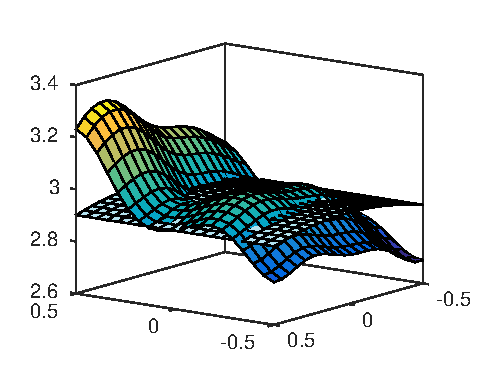
\includegraphics{plots/experiments/2dof/g11_hat.eps}
		%\caption{$\hat{W}_\varphi(t)$}
	\end{subfigure}
	\begin{subfigure}{0.5\textwidth}
		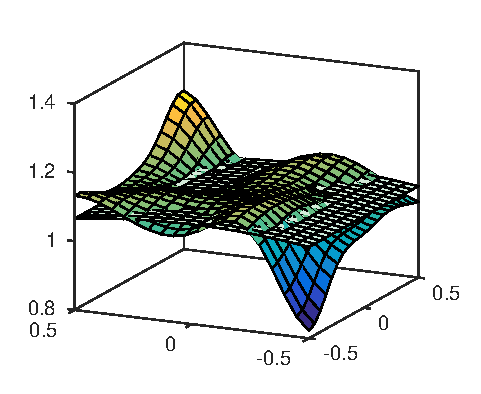
\includegraphics{plots/experiments/2dof/g12_hat.eps}
		%\caption{$\hat{W}_\gamma(t)$)}
	\end{subfigure}
	\caption{Σύγκριση των συναρτήσεων $\gamma_{11}(x)$ (αριστερά) και $\gamma_{12}(x)$ (δεξιά) με τις προσεγγίσεις τους $\hat{\gamma}_{11}(x)$ και $\hat{\gamma}_{12}(x)$ αντίστοιχα. Με γκρι (transparent) απεικονίζονται οι πραγματικές συναρτήσεις ενώ οι χρωματισμένες επιφάνειες είναι οι προσεγγίσεις αυτών. }
	\label{fig:2dof_g1_approximations}
\end{figure}

\begin{figure}
	\begin{subfigure}{0.5\textwidth}
		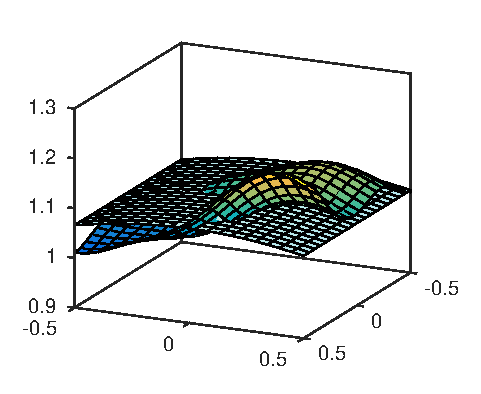
\includegraphics{plots/experiments/2dof/g21_hat.eps}
		%\caption{$\hat{W}_\varphi(t)$}
	\end{subfigure}
	\begin{subfigure}{0.5\textwidth}
		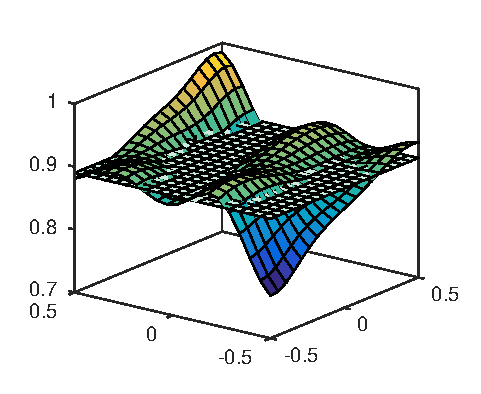
\includegraphics{plots/experiments/2dof/g22_hat.eps}
		%\caption{$\hat{W}_\gamma(t)$)}
	\end{subfigure}
	\caption{Σύγκριση των συναρτήσεων $\gamma_{21}(x)$ (αριστερά) και $\gamma_{22}(x)$ (δεξιά) με τις προσεγγίσεις τους $\hat{\gamma}_{21}(x)$ και $\hat{\gamma}_{22}(x)$ αντίστοιχα. Με γκρι (transparent) απεικονίζονται οι πραγματικές συναρτήσεις ενώ οι χρωματισμένες επιφάνειες είναι οι προσεγγίσεις αυτών. }
	\label{fig:2dof_g2_approximations}
\end{figure}


\section{Παρατηρήσεις}
\label{eq:remarks_on_exp}
Τέλος, σε αυτή την ενότητα παρουσιάζονται κάποιες παρατηρήσεις με βάση τα πειράματα που παρουσιάστηκαν στις Ενότητες \ref{sec:rbf_experiments} και \ref{sec:real_system_experiments}.\\

\begin{remark}
	Ο ρυθμός και η τελική ζώνη σύγκλισης των παραμετρικών σφαλμάτων $\tilde{W}(t)$ είναι άγνωστος και εξαρτάται από τις τιμές τόσο των κερδών $\beta_i$ όσο και από τα άγνωστα επίπεδα διέγερσης $a_1$ και $a_2$. Η βελτιστοποίηση αυτών των χαρακτηριστικών της διαδικασίας εκμάθησης μέσω ρύθμισης των παραμέτρων του σχήματος αναγνώρισης είναι μια δύσκολη διαδικασία καθώς δεν είναι ξεκάθαρο με ποιόν τρόπο επιδρά η κάθε παράμετρος στα άγνωστα επίπεδα διέγερσης.
	
	Για παράδειγμα, στο Πείραμα \ref{exampleB} φαίνεται πως τα βάρη δεν συγκλίνουν στις ακριβές τιμές τους αλλά σε μια περιοχή αυτών, και ως αποτέλεσμα οι προσεγγίσεις των συναρτήσεων $\gamma_{ij}(x)$ καταφέρνουν να προσεγγίσουν τις άγνωστες συναρτήσεις μόνο κατά μέση τιμή. Καθώς το πλάτος της περιοχής σύγκλισης εξαρτάται από τα άγνωστα επίπεδα διέγερσης, είναι δύσκολη η εύρεση παραμέτρων που θα επιφέρουν καλύτερα αποτελέσματα.\\
\end{remark}

\begin{remark}
	Το σχήμα αναγνώρισης είναι αρκετά απαιτητικό από υπολογιστικής άποψης. Το γεγονός αυτό, γίνεται εμφανές εάν θεωρήσει κανείς την διαδικασία αναγνώρισης ενός συστήματος ΠΕΠΕ.
	
	Για παράδειγμα, στο Πείραμα \ref{exampleB} προσεγγίζουμε τις άγνωστες συναρτήσεις με RBF δίκτυα τα οποία έχουν κέντρα σε ένα πλέγμα, όπου σε κάθε διάσταση τοποθετούνται 5 κέντρα. Ως αποτέλεσμα, για την αναγνώριση κάθε συνάρτησης $\varphi(x)$ χρειαζόμαστε $5^4$ βάρη, τα οποία υπολογίζονται κατά την διάρκεια του πειράματος μέσω αριθμητικής επίλυσης των διαφορικών εξισώσεων που ορίζουν οι νόμοι προσαρμογής. Μόνο για το διάνυσμα $\Phi$, απαιτείται η επίλυση $1250$ τέτοιων διαφορικών εξισώσεων. Επιπλέον, το μέγεθος της περιόδου είναι αρκετά μεγάλο, καθώς σε κάθε περίοδο πρέπει να επισκεφθούμε κάθε ένα από αυτά τα 650 κέντρα.
	
	Αν ωστόσο προσπαθούσαμε να προσεγγίσουμε με την ίδια στρατηγική έναν βραχίονα τριών βαθμών ελευθερίας το οποίο είναι ένα σύστημα έξι καταστάσεων, τότε μόνο για την αναγνώριση του διανύσματος $\Phi(x)$ θα απαιτούταν $3 \cdot 5^6 = 46875$ βάρη. Επίσης η περίοδος θα μεγάλωνε σε διάρκεια $25$ φορές, αφού πλέον θα πρέπει να επισκεφθούμε ακόμα περισσότερα κέντρα.
	
	Όπως είναι προφανές από τον παραπάνω συνειρμό, η εφαρμογή του σχήματος ελέγχου σε συστήματα μεγάλων διαστάσεων απαιτεί τεράστιους υπολογιστικούς πόρους.\\
\end{remark}

\begin{remark}
	\label{remakr:border_eval}
	Ενώ το σχήμα αναγνώρισης συνήθως παράγει αρκετά καλές εκτιμήσεις στο εσωτερικό του $\Omega_x$, οι προσεγγίσεις των συναρτήσεων φαίνεται να χάνουν ακρίβεια στο σύνορο του $\Omega_x$. Το φαινόμενο αυτό παρατηρείται τόσο στο Πείραμα \ref{exp:vdp} (ταλαντωτής \textit{Van Der Pol}) όσο και στο Πείραμα \ref{exampleB} (ρομποτικός βραχίονας). Σχετικά με αυτό το πρόβλημα παρουσιάζεται μια λύση στο Κεφάλαιο \ref{chap:conclusions}. \\
\end{remark}

\begin{remark}
	Από το Πείραμα \ref{exp:vdp} φαίνεται πως το σχήμα αναγνώρισης είναι ικανό να αναγνωρίσει συστήματα που δεν εμπίπτουν στην κατηγορία \textit{Euler Lagrange}. Ωστόσο, καθώς το πείραμα αυτό αποτελεί μεμονωμένο παράδειγμα, δεν μπορούμε να προχωρήσουμε στο συμπέρασμα ότι το σχήμα είναι ικανό να αναγνωρίσει κάθε τέτοιο σύστημα, συνεπώς απαιτείται επιπλέον έρευνα για την συγκεκριμένη υπόθεση.
\end{remark}